\documentclass[twoside]{book}

% Packages required by doxygen
\usepackage{fixltx2e}
\usepackage{calc}
\usepackage{doxygen}
\usepackage[export]{adjustbox} % also loads graphicx
\usepackage{graphicx}
\usepackage[utf8]{inputenc}
\usepackage{makeidx}
\usepackage{multicol}
\usepackage{multirow}
\PassOptionsToPackage{warn}{textcomp}
\usepackage{textcomp}
\usepackage[nointegrals]{wasysym}
\usepackage[table]{xcolor}

% Font selection
\usepackage[T1]{fontenc}
\usepackage[scaled=.90]{helvet}
\usepackage{courier}
\usepackage{amssymb}
\usepackage{sectsty}
\renewcommand{\familydefault}{\sfdefault}
\allsectionsfont{%
  \fontseries{bc}\selectfont%
  \color{darkgray}%
}
\renewcommand{\DoxyLabelFont}{%
  \fontseries{bc}\selectfont%
  \color{darkgray}%
}
\newcommand{\+}{\discretionary{\mbox{\scriptsize$\hookleftarrow$}}{}{}}

% Page & text layout
\usepackage{geometry}
\geometry{%
  a4paper,%
  top=2.5cm,%
  bottom=2.5cm,%
  left=2.5cm,%
  right=2.5cm%
}
\tolerance=750
\hfuzz=15pt
\hbadness=750
\setlength{\emergencystretch}{15pt}
\setlength{\parindent}{0cm}
\setlength{\parskip}{3ex plus 2ex minus 2ex}
\makeatletter
\renewcommand{\paragraph}{%
  \@startsection{paragraph}{4}{0ex}{-1.0ex}{1.0ex}{%
    \normalfont\normalsize\bfseries\SS@parafont%
  }%
}
\renewcommand{\subparagraph}{%
  \@startsection{subparagraph}{5}{0ex}{-1.0ex}{1.0ex}{%
    \normalfont\normalsize\bfseries\SS@subparafont%
  }%
}
\makeatother

% Headers & footers
\usepackage{fancyhdr}
\pagestyle{fancyplain}
\fancyhead[LE]{\fancyplain{}{\bfseries\thepage}}
\fancyhead[CE]{\fancyplain{}{}}
\fancyhead[RE]{\fancyplain{}{\bfseries\leftmark}}
\fancyhead[LO]{\fancyplain{}{\bfseries\rightmark}}
\fancyhead[CO]{\fancyplain{}{}}
\fancyhead[RO]{\fancyplain{}{\bfseries\thepage}}
\fancyfoot[LE]{\fancyplain{}{}}
\fancyfoot[CE]{\fancyplain{}{}}
\fancyfoot[RE]{\fancyplain{}{\bfseries\scriptsize Generated by Doxygen }}
\fancyfoot[LO]{\fancyplain{}{\bfseries\scriptsize Generated by Doxygen }}
\fancyfoot[CO]{\fancyplain{}{}}
\fancyfoot[RO]{\fancyplain{}{}}
\renewcommand{\footrulewidth}{0.4pt}
\renewcommand{\chaptermark}[1]{%
  \markboth{#1}{}%
}
\renewcommand{\sectionmark}[1]{%
  \markright{\thesection\ #1}%
}

% Indices & bibliography
\usepackage{natbib}
\usepackage[titles]{tocloft}
\setcounter{tocdepth}{3}
\setcounter{secnumdepth}{5}
\makeindex

% Hyperlinks (required, but should be loaded last)
\usepackage{ifpdf}
\ifpdf
  \usepackage[pdftex,pagebackref=true]{hyperref}
\else
  \usepackage[ps2pdf,pagebackref=true]{hyperref}
\fi
\hypersetup{%
  colorlinks=true,%
  linkcolor=blue,%
  citecolor=blue,%
  unicode%
}

% Custom commands
\newcommand{\clearemptydoublepage}{%
  \newpage{\pagestyle{empty}\cleardoublepage}%
}

\usepackage{caption}
\captionsetup{labelsep=space,justification=centering,font={bf},singlelinecheck=off,skip=4pt,position=top}

%===== C O N T E N T S =====

\begin{document}

% Titlepage & ToC
\hypersetup{pageanchor=false,
             bookmarksnumbered=true,
             pdfencoding=unicode
            }
\pagenumbering{roman}
\begin{titlepage}
\vspace*{7cm}
\begin{center}%
{\Large Petit\+Prince Server \\[1ex]\large 1.\+0 }\\
\vspace*{1cm}
{\large Generated by Doxygen 1.8.11}\\
\end{center}
\end{titlepage}
\clearemptydoublepage
\tableofcontents
\clearemptydoublepage
\pagenumbering{arabic}
\hypersetup{pageanchor=true}

%--- Begin generated contents ---
\chapter{Hierarchical Index}
\section{Class Hierarchy}
This inheritance list is sorted roughly, but not completely, alphabetically\+:\begin{DoxyCompactList}
\item \contentsline{section}{\+\_\+0\+R\+L\+\_\+insert\+To\+Any\+\_\+\+Singleton\+\_\+\+\_\+c\+Petit\+Prince\+\_\+m\+Draw\+Service\+\_\+m\+Non\+Applicable}{\pageref{class__0_r_l__insert_to_any___singleton____c_petit_prince__m_draw_service__m_non_applicable}}{}
\item \contentsline{section}{\+\_\+0\+R\+L\+\_\+insert\+To\+Any\+\_\+\+Singleton\+\_\+\+\_\+c\+Petit\+Prince\+\_\+m\+Draw\+Service\+\_\+m\+Unexpected\+Draw}{\pageref{class__0_r_l__insert_to_any___singleton____c_petit_prince__m_draw_service__m_unexpected_draw}}{}
\item \contentsline{section}{\+\_\+0\+R\+L\+\_\+insert\+To\+Any\+\_\+\+Singleton\+\_\+\+\_\+c\+Petit\+Prince\+\_\+m\+Petit\+Prince\+Service\+\_\+m\+Invalid\+Draw\+Params}{\pageref{class__0_r_l__insert_to_any___singleton____c_petit_prince__m_petit_prince_service__m_invalid_draw_params}}{}
\item \+\_\+\+C\+O\+R\+B\+A\+\_\+\+Unbounded\+\_\+\+Sequence\begin{DoxyCompactList}
\item \contentsline{section}{Point\+Seq}{\pageref{class_point_seq}}{}
\end{DoxyCompactList}
\item \+\_\+\+C\+O\+R\+B\+A\+\_\+\+Unbounded\+\_\+\+Sequence\+\_\+\+Value\begin{DoxyCompactList}
\item \contentsline{section}{Draw\+Seq}{\pageref{class_draw_seq}}{}
\end{DoxyCompactList}
\item \+\_\+\+C\+O\+R\+B\+A\+\_\+\+Unbounded\+\_\+\+Sequence\+\_\+w\+\_\+\+Fix\+Size\+Element\begin{DoxyCompactList}
\item \contentsline{section}{Long\+Seq}{\pageref{class_long_seq}}{}
\end{DoxyCompactList}
\item \+\_\+impl\+\_\+\+Draw\+Service\begin{DoxyCompactList}
\item \contentsline{section}{Draw\+Service}{\pageref{class_draw_service}}{}
\end{DoxyCompactList}
\item \+\_\+impl\+\_\+\+Petit\+Prince\+Service\begin{DoxyCompactList}
\item \contentsline{section}{Petit\+Prince\+Service}{\pageref{class_petit_prince_service}}{}
\end{DoxyCompactList}
\item \+\_\+\+O\+M\+N\+I\+\_\+\+N\+Sproxy\+Object\+Factory\begin{DoxyCompactList}
\item \contentsline{section}{\+\_\+pof\+\_\+\+Draw\+Service}{\pageref{class__pof___draw_service}}{}
\item \contentsline{section}{\+\_\+pof\+\_\+\+Petit\+Prince\+Service}{\pageref{class__pof___petit_prince_service}}{}
\end{DoxyCompactList}
\item Circle\begin{DoxyCompactList}
\item \contentsline{section}{Circle}{\pageref{class_circle}}{}
\end{DoxyCompactList}
\item \contentsline{section}{Circle\+\_\+\+Helper}{\pageref{class_circle___helper}}{}
\item Draw\begin{DoxyCompactList}
\item \contentsline{section}{Draw}{\pageref{class_draw}}{}
\begin{DoxyCompactList}
\item \contentsline{section}{Circle}{\pageref{class_circle}}{}
\item \contentsline{section}{Circle}{\pageref{class_circle}}{}
\item \contentsline{section}{Ellipse}{\pageref{class_ellipse}}{}
\item \contentsline{section}{Ellipse}{\pageref{class_ellipse}}{}
\item \contentsline{section}{Line}{\pageref{class_line}}{}
\item \contentsline{section}{Line}{\pageref{class_line}}{}
\item \contentsline{section}{Polygon}{\pageref{class_polygon}}{}
\item \contentsline{section}{Polygon}{\pageref{class_polygon}}{}
\end{DoxyCompactList}
\end{DoxyCompactList}
\item \contentsline{section}{Draw\+\_\+\+Helper}{\pageref{class_draw___helper}}{}
\item \contentsline{section}{Draw\+Seq\+\_\+out}{\pageref{class_draw_seq__out}}{}
\item \contentsline{section}{Draw\+Seq\+\_\+var}{\pageref{class_draw_seq__var}}{}
\item Draw\+Service\begin{DoxyCompactList}
\item \contentsline{section}{Draw\+Service\+Impl}{\pageref{class_draw_service_impl}}{}
\end{DoxyCompactList}
\item \contentsline{section}{Draw\+Service\+\_\+\+Helper}{\pageref{class_draw_service___helper}}{}
\item Ellipse\begin{DoxyCompactList}
\item \contentsline{section}{Ellipse}{\pageref{class_ellipse}}{}
\end{DoxyCompactList}
\item \contentsline{section}{Ellipse\+\_\+\+Helper}{\pageref{class_ellipse___helper}}{}
\item Line\begin{DoxyCompactList}
\item \contentsline{section}{Line}{\pageref{class_line}}{}
\end{DoxyCompactList}
\item \contentsline{section}{Line\+\_\+\+Helper}{\pageref{class_line___helper}}{}
\item \contentsline{section}{Long\+Seq\+\_\+out}{\pageref{class_long_seq__out}}{}
\item \contentsline{section}{Long\+Seq\+\_\+var}{\pageref{class_long_seq__var}}{}
\item Object\begin{DoxyCompactList}
\item \contentsline{section}{\+\_\+objref\+\_\+\+Draw\+Service}{\pageref{class__objref___draw_service}}{}
\item \contentsline{section}{\+\_\+objref\+\_\+\+Petit\+Prince\+Service}{\pageref{class__objref___petit_prince_service}}{}
\end{DoxyCompactList}
\item omni\+Call\+Descriptor\begin{DoxyCompactList}
\item \contentsline{section}{\+\_\+0\+R\+L\+\_\+cd\+\_\+c93297503b4b476c\+\_\+00000000}{\pageref{class__0_r_l__cd__c93297503b4b476c__00000000}}{}
\item \contentsline{section}{\+\_\+0\+R\+L\+\_\+cd\+\_\+c93297503b4b476c\+\_\+11000000}{\pageref{class__0_r_l__cd__c93297503b4b476c__11000000}}{}
\item \contentsline{section}{\+\_\+0\+R\+L\+\_\+cd\+\_\+c93297503b4b476c\+\_\+30000000}{\pageref{class__0_r_l__cd__c93297503b4b476c__30000000}}{}
\item \contentsline{section}{\+\_\+0\+R\+L\+\_\+cd\+\_\+c93297503b4b476c\+\_\+31000000}{\pageref{class__0_r_l__cd__c93297503b4b476c__31000000}}{}
\item \contentsline{section}{\+\_\+0\+R\+L\+\_\+cd\+\_\+c93297503b4b476c\+\_\+50000000}{\pageref{class__0_r_l__cd__c93297503b4b476c__50000000}}{}
\item \contentsline{section}{\+\_\+0\+R\+L\+\_\+cd\+\_\+c93297503b4b476c\+\_\+51000000}{\pageref{class__0_r_l__cd__c93297503b4b476c__51000000}}{}
\item \contentsline{section}{\+\_\+0\+R\+L\+\_\+cd\+\_\+c93297503b4b476c\+\_\+71000000}{\pageref{class__0_r_l__cd__c93297503b4b476c__71000000}}{}
\item \contentsline{section}{\+\_\+0\+R\+L\+\_\+cd\+\_\+c93297503b4b476c\+\_\+80000000}{\pageref{class__0_r_l__cd__c93297503b4b476c__80000000}}{}
\item \contentsline{section}{\+\_\+0\+R\+L\+\_\+cd\+\_\+c93297503b4b476c\+\_\+91000000}{\pageref{class__0_r_l__cd__c93297503b4b476c__91000000}}{}
\item \contentsline{section}{\+\_\+0\+R\+L\+\_\+cd\+\_\+c93297503b4b476c\+\_\+b0000000}{\pageref{class__0_r_l__cd__c93297503b4b476c__b0000000}}{}
\item \contentsline{section}{\+\_\+0\+R\+L\+\_\+cd\+\_\+c93297503b4b476c\+\_\+d0000000}{\pageref{class__0_r_l__cd__c93297503b4b476c__d0000000}}{}
\item \contentsline{section}{\+\_\+0\+R\+L\+\_\+cd\+\_\+c93297503b4b476c\+\_\+f0000000}{\pageref{class__0_r_l__cd__c93297503b4b476c__f0000000}}{}
\end{DoxyCompactList}
\item omni\+Obj\+Ref\begin{DoxyCompactList}
\item \contentsline{section}{\+\_\+objref\+\_\+\+Draw\+Service}{\pageref{class__objref___draw_service}}{}
\item \contentsline{section}{\+\_\+objref\+\_\+\+Petit\+Prince\+Service}{\pageref{class__objref___petit_prince_service}}{}
\end{DoxyCompactList}
\item omni\+Servant\begin{DoxyCompactList}
\item \contentsline{section}{\+\_\+impl\+\_\+\+Draw\+Service}{\pageref{class__impl___draw_service}}{}
\item \contentsline{section}{\+\_\+impl\+\_\+\+Petit\+Prince\+Service}{\pageref{class__impl___petit_prince_service}}{}
\end{DoxyCompactList}
\item Petit\+Prince\+Service\begin{DoxyCompactList}
\item \contentsline{section}{Petit\+Prince\+Service\+Impl}{\pageref{class_petit_prince_service_impl}}{}
\end{DoxyCompactList}
\item \contentsline{section}{Petit\+Prince\+Service\+\_\+\+Helper}{\pageref{class_petit_prince_service___helper}}{}
\item \contentsline{section}{Point}{\pageref{struct_point}}{}
\item \contentsline{section}{Point\+Seq\+\_\+out}{\pageref{class_point_seq__out}}{}
\item \contentsline{section}{Point\+Seq\+\_\+var}{\pageref{class_point_seq__var}}{}
\item Polygon\begin{DoxyCompactList}
\item \contentsline{section}{Polygon}{\pageref{class_polygon}}{}
\end{DoxyCompactList}
\item \contentsline{section}{Polygon\+\_\+\+Helper}{\pageref{class_polygon___helper}}{}
\item Ref\+Count\+Servant\+Base\begin{DoxyCompactList}
\item \contentsline{section}{Draw\+Service\+Impl}{\pageref{class_draw_service_impl}}{}
\item \contentsline{section}{Petit\+Prince\+Service\+Impl}{\pageref{class_petit_prince_service_impl}}{}
\end{DoxyCompactList}
\item Servant\+Base\begin{DoxyCompactList}
\item \contentsline{section}{Draw\+Service}{\pageref{class_draw_service}}{}
\item \contentsline{section}{Petit\+Prince\+Service}{\pageref{class_petit_prince_service}}{}
\end{DoxyCompactList}
\item User\+Exception\begin{DoxyCompactList}
\item \contentsline{section}{Draw\+Service\+:\+:Non\+Applicable}{\pageref{class_draw_service_1_1_non_applicable}}{}
\item \contentsline{section}{Draw\+Service\+:\+:Unexpected\+Draw}{\pageref{class_draw_service_1_1_unexpected_draw}}{}
\item \contentsline{section}{Petit\+Prince\+Service\+:\+:Invalid\+Draw\+Params}{\pageref{class_petit_prince_service_1_1_invalid_draw_params}}{}
\end{DoxyCompactList}
\item Value\+Base\begin{DoxyCompactList}
\item \contentsline{section}{Draw}{\pageref{class_draw}}{}
\end{DoxyCompactList}
\end{DoxyCompactList}

\chapter{Class Index}
\section{Class List}
Here are the classes, structs, unions and interfaces with brief descriptions\+:\begin{DoxyCompactList}
\item\contentsline{section}{\hyperlink{class__0_r_l__cd__c93297503b4b476c__00000000}{\+\_\+0\+R\+L\+\_\+cd\+\_\+c93297503b4b476c\+\_\+00000000} }{\pageref{class__0_r_l__cd__c93297503b4b476c__00000000}}{}
\item\contentsline{section}{\hyperlink{class__0_r_l__cd__c93297503b4b476c__11000000}{\+\_\+0\+R\+L\+\_\+cd\+\_\+c93297503b4b476c\+\_\+11000000} }{\pageref{class__0_r_l__cd__c93297503b4b476c__11000000}}{}
\item\contentsline{section}{\hyperlink{class__0_r_l__cd__c93297503b4b476c__30000000}{\+\_\+0\+R\+L\+\_\+cd\+\_\+c93297503b4b476c\+\_\+30000000} }{\pageref{class__0_r_l__cd__c93297503b4b476c__30000000}}{}
\item\contentsline{section}{\hyperlink{class__0_r_l__cd__c93297503b4b476c__31000000}{\+\_\+0\+R\+L\+\_\+cd\+\_\+c93297503b4b476c\+\_\+31000000} }{\pageref{class__0_r_l__cd__c93297503b4b476c__31000000}}{}
\item\contentsline{section}{\hyperlink{class__0_r_l__cd__c93297503b4b476c__50000000}{\+\_\+0\+R\+L\+\_\+cd\+\_\+c93297503b4b476c\+\_\+50000000} }{\pageref{class__0_r_l__cd__c93297503b4b476c__50000000}}{}
\item\contentsline{section}{\hyperlink{class__0_r_l__cd__c93297503b4b476c__51000000}{\+\_\+0\+R\+L\+\_\+cd\+\_\+c93297503b4b476c\+\_\+51000000} }{\pageref{class__0_r_l__cd__c93297503b4b476c__51000000}}{}
\item\contentsline{section}{\hyperlink{class__0_r_l__cd__c93297503b4b476c__71000000}{\+\_\+0\+R\+L\+\_\+cd\+\_\+c93297503b4b476c\+\_\+71000000} }{\pageref{class__0_r_l__cd__c93297503b4b476c__71000000}}{}
\item\contentsline{section}{\hyperlink{class__0_r_l__cd__c93297503b4b476c__80000000}{\+\_\+0\+R\+L\+\_\+cd\+\_\+c93297503b4b476c\+\_\+80000000} }{\pageref{class__0_r_l__cd__c93297503b4b476c__80000000}}{}
\item\contentsline{section}{\hyperlink{class__0_r_l__cd__c93297503b4b476c__91000000}{\+\_\+0\+R\+L\+\_\+cd\+\_\+c93297503b4b476c\+\_\+91000000} }{\pageref{class__0_r_l__cd__c93297503b4b476c__91000000}}{}
\item\contentsline{section}{\hyperlink{class__0_r_l__cd__c93297503b4b476c__b0000000}{\+\_\+0\+R\+L\+\_\+cd\+\_\+c93297503b4b476c\+\_\+b0000000} }{\pageref{class__0_r_l__cd__c93297503b4b476c__b0000000}}{}
\item\contentsline{section}{\hyperlink{class__0_r_l__cd__c93297503b4b476c__d0000000}{\+\_\+0\+R\+L\+\_\+cd\+\_\+c93297503b4b476c\+\_\+d0000000} }{\pageref{class__0_r_l__cd__c93297503b4b476c__d0000000}}{}
\item\contentsline{section}{\hyperlink{class__0_r_l__cd__c93297503b4b476c__f0000000}{\+\_\+0\+R\+L\+\_\+cd\+\_\+c93297503b4b476c\+\_\+f0000000} }{\pageref{class__0_r_l__cd__c93297503b4b476c__f0000000}}{}
\item\contentsline{section}{\hyperlink{class__0_r_l__insert_to_any___singleton____c_petit_prince__m_draw_service__m_non_applicable}{\+\_\+0\+R\+L\+\_\+insert\+To\+Any\+\_\+\+Singleton\+\_\+\+\_\+c\+Petit\+Prince\+\_\+m\+Draw\+Service\+\_\+m\+Non\+Applicable} }{\pageref{class__0_r_l__insert_to_any___singleton____c_petit_prince__m_draw_service__m_non_applicable}}{}
\item\contentsline{section}{\hyperlink{class__0_r_l__insert_to_any___singleton____c_petit_prince__m_draw_service__m_unexpected_draw}{\+\_\+0\+R\+L\+\_\+insert\+To\+Any\+\_\+\+Singleton\+\_\+\+\_\+c\+Petit\+Prince\+\_\+m\+Draw\+Service\+\_\+m\+Unexpected\+Draw} }{\pageref{class__0_r_l__insert_to_any___singleton____c_petit_prince__m_draw_service__m_unexpected_draw}}{}
\item\contentsline{section}{\hyperlink{class__0_r_l__insert_to_any___singleton____c_petit_prince__m_petit_prince_service__m_invalid_draw_params}{\+\_\+0\+R\+L\+\_\+insert\+To\+Any\+\_\+\+Singleton\+\_\+\+\_\+c\+Petit\+Prince\+\_\+m\+Petit\+Prince\+Service\+\_\+m\+Invalid\+Draw\+Params} }{\pageref{class__0_r_l__insert_to_any___singleton____c_petit_prince__m_petit_prince_service__m_invalid_draw_params}}{}
\item\contentsline{section}{\hyperlink{class__impl___draw_service}{\+\_\+impl\+\_\+\+Draw\+Service} }{\pageref{class__impl___draw_service}}{}
\item\contentsline{section}{\hyperlink{class__impl___petit_prince_service}{\+\_\+impl\+\_\+\+Petit\+Prince\+Service} }{\pageref{class__impl___petit_prince_service}}{}
\item\contentsline{section}{\hyperlink{class__objref___draw_service}{\+\_\+objref\+\_\+\+Draw\+Service} }{\pageref{class__objref___draw_service}}{}
\item\contentsline{section}{\hyperlink{class__objref___petit_prince_service}{\+\_\+objref\+\_\+\+Petit\+Prince\+Service} }{\pageref{class__objref___petit_prince_service}}{}
\item\contentsline{section}{\hyperlink{class__pof___draw_service}{\+\_\+pof\+\_\+\+Draw\+Service} }{\pageref{class__pof___draw_service}}{}
\item\contentsline{section}{\hyperlink{class__pof___petit_prince_service}{\+\_\+pof\+\_\+\+Petit\+Prince\+Service} }{\pageref{class__pof___petit_prince_service}}{}
\item\contentsline{section}{\hyperlink{class_circle}{Circle} }{\pageref{class_circle}}{}
\item\contentsline{section}{\hyperlink{class_circle___helper}{Circle\+\_\+\+Helper} }{\pageref{class_circle___helper}}{}
\item\contentsline{section}{\hyperlink{class_draw}{Draw} \\*This class is a virtual class that define the first behavior of each draws that will be implemented }{\pageref{class_draw}}{}
\item\contentsline{section}{\hyperlink{class_draw___helper}{Draw\+\_\+\+Helper} }{\pageref{class_draw___helper}}{}
\item\contentsline{section}{\hyperlink{class_draw_seq}{Draw\+Seq} }{\pageref{class_draw_seq}}{}
\item\contentsline{section}{\hyperlink{class_draw_seq__out}{Draw\+Seq\+\_\+out} }{\pageref{class_draw_seq__out}}{}
\item\contentsline{section}{\hyperlink{class_draw_seq__var}{Draw\+Seq\+\_\+var} }{\pageref{class_draw_seq__var}}{}
\item\contentsline{section}{\hyperlink{class_draw_service}{Draw\+Service} }{\pageref{class_draw_service}}{}
\item\contentsline{section}{\hyperlink{class_draw_service___helper}{Draw\+Service\+\_\+\+Helper} }{\pageref{class_draw_service___helper}}{}
\item\contentsline{section}{\hyperlink{class_draw_service_impl}{Draw\+Service\+Impl} \\*This class implements the \hyperlink{class_draw_service}{Draw\+Service} interface generated by the idl after compilation. The \hyperlink{class_draw_service}{Draw\+Service} class inherited is the P\+OA version. The P\+OA classes inherit the {\itshape impl} classes which inherit the interfaces. This class will define the implementation of each methods contained in the interface (see cpp source file) }{\pageref{class_draw_service_impl}}{}
\item\contentsline{section}{\hyperlink{class_ellipse}{Ellipse} }{\pageref{class_ellipse}}{}
\item\contentsline{section}{\hyperlink{class_ellipse___helper}{Ellipse\+\_\+\+Helper} }{\pageref{class_ellipse___helper}}{}
\item\contentsline{section}{\hyperlink{class_petit_prince_service_1_1_invalid_draw_params}{Petit\+Prince\+Service\+::\+Invalid\+Draw\+Params} }{\pageref{class_petit_prince_service_1_1_invalid_draw_params}}{}
\item\contentsline{section}{\hyperlink{class_line}{Line} \\*This class is the class that define the implementation of a circle }{\pageref{class_line}}{}
\item\contentsline{section}{\hyperlink{class_line___helper}{Line\+\_\+\+Helper} }{\pageref{class_line___helper}}{}
\item\contentsline{section}{\hyperlink{class_long_seq}{Long\+Seq} }{\pageref{class_long_seq}}{}
\item\contentsline{section}{\hyperlink{class_long_seq__out}{Long\+Seq\+\_\+out} }{\pageref{class_long_seq__out}}{}
\item\contentsline{section}{\hyperlink{class_long_seq__var}{Long\+Seq\+\_\+var} }{\pageref{class_long_seq__var}}{}
\item\contentsline{section}{\hyperlink{class_draw_service_1_1_non_applicable}{Draw\+Service\+::\+Non\+Applicable} }{\pageref{class_draw_service_1_1_non_applicable}}{}
\item\contentsline{section}{\hyperlink{class_petit_prince_service}{Petit\+Prince\+Service} }{\pageref{class_petit_prince_service}}{}
\item\contentsline{section}{\hyperlink{class_petit_prince_service___helper}{Petit\+Prince\+Service\+\_\+\+Helper} }{\pageref{class_petit_prince_service___helper}}{}
\item\contentsline{section}{\hyperlink{class_petit_prince_service_impl}{Petit\+Prince\+Service\+Impl} \\*This class implements the \hyperlink{class_petit_prince_service}{Petit\+Prince\+Service} interface generated by the idl after compilation. The \hyperlink{class_petit_prince_service}{Petit\+Prince\+Service} class inherited is the P\+OA version. The P\+OA classes inherit the {\itshape impl} classes which inherit the interfaces. This class will define the implementation of each methods contained in the interface (see cpp source file) }{\pageref{class_petit_prince_service_impl}}{}
\item\contentsline{section}{\hyperlink{struct_point}{Point} }{\pageref{struct_point}}{}
\item\contentsline{section}{\hyperlink{class_point_seq}{Point\+Seq} }{\pageref{class_point_seq}}{}
\item\contentsline{section}{\hyperlink{class_point_seq__out}{Point\+Seq\+\_\+out} }{\pageref{class_point_seq__out}}{}
\item\contentsline{section}{\hyperlink{class_point_seq__var}{Point\+Seq\+\_\+var} }{\pageref{class_point_seq__var}}{}
\item\contentsline{section}{\hyperlink{class_polygon}{Polygon} }{\pageref{class_polygon}}{}
\item\contentsline{section}{\hyperlink{class_polygon___helper}{Polygon\+\_\+\+Helper} }{\pageref{class_polygon___helper}}{}
\item\contentsline{section}{\hyperlink{class_draw_service_1_1_unexpected_draw}{Draw\+Service\+::\+Unexpected\+Draw} }{\pageref{class_draw_service_1_1_unexpected_draw}}{}
\end{DoxyCompactList}

\chapter{File Index}
\section{File List}
Here is a list of all files with brief descriptions\+:\begin{DoxyCompactList}
\item\contentsline{section}{\hyperlink{_8dep_8inc}{.\+dep.\+inc} }{\pageref{_8dep_8inc}}{}
\item\contentsline{section}{\hyperlink{main__client_8cpp}{main\+\_\+client.\+cpp} \\*Define the client main }{\pageref{main__client_8cpp}}{}
\item\contentsline{section}{build/\+Debug/\+G\+N\+U-\/\+Linux/\hyperlink{main__client_8o_8d}{main\+\_\+client.\+o.\+d} }{\pageref{main__client_8o_8d}}{}
\item\contentsline{section}{build/\+Debug/\+G\+N\+U-\/\+Linux/src/\hyperlink{_petit_prince___dyn_stub_8o_8d}{Petit\+Prince\+\_\+\+Dyn\+Stub.\+o.\+d} }{\pageref{_petit_prince___dyn_stub_8o_8d}}{}
\item\contentsline{section}{build/\+Debug/\+G\+N\+U-\/\+Linux/src/\hyperlink{_petit_prince___stub_8o_8d}{Petit\+Prince\+\_\+\+Stub.\+o.\+d} }{\pageref{_petit_prince___stub_8o_8d}}{}
\item\contentsline{section}{hdr/\hyperlink{_draw_service_impl_8hpp}{Draw\+Service\+Impl.\+hpp} }{\pageref{_draw_service_impl_8hpp}}{}
\item\contentsline{section}{hdr/\hyperlink{_petit_prince_8hpp}{Petit\+Prince.\+hpp} }{\pageref{_petit_prince_8hpp}}{}
\item\contentsline{section}{hdr/\hyperlink{_petit_prince_service_impl_8hpp}{Petit\+Prince\+Service\+Impl.\+hpp} }{\pageref{_petit_prince_service_impl_8hpp}}{}
\item\contentsline{section}{src/\hyperlink{_petit_prince___dyn_stub_8cpp}{Petit\+Prince\+\_\+\+Dyn\+Stub.\+cpp} }{\pageref{_petit_prince___dyn_stub_8cpp}}{}
\item\contentsline{section}{src/\hyperlink{_petit_prince___stub_8cpp}{Petit\+Prince\+\_\+\+Stub.\+cpp} }{\pageref{_petit_prince___stub_8cpp}}{}
\end{DoxyCompactList}

\chapter{Class Documentation}
\hypertarget{class__0_r_l__cd__c93297503b4b476c__00000000}{}\section{\+\_\+0\+R\+L\+\_\+cd\+\_\+c93297503b4b476c\+\_\+00000000 Class Reference}
\label{class__0_r_l__cd__c93297503b4b476c__00000000}\index{\+\_\+0\+R\+L\+\_\+cd\+\_\+c93297503b4b476c\+\_\+00000000@{\+\_\+0\+R\+L\+\_\+cd\+\_\+c93297503b4b476c\+\_\+00000000}}


Inheritance diagram for \+\_\+0\+R\+L\+\_\+cd\+\_\+c93297503b4b476c\+\_\+00000000\+:
\nopagebreak
\begin{figure}[H]
\begin{center}
\leavevmode
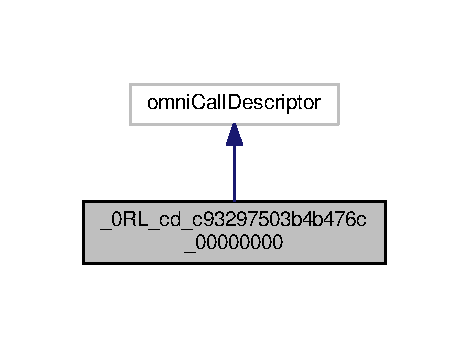
\includegraphics[width=225pt]{class__0_r_l__cd__c93297503b4b476c__00000000__inherit__graph}
\end{center}
\end{figure}


Collaboration diagram for \+\_\+0\+R\+L\+\_\+cd\+\_\+c93297503b4b476c\+\_\+00000000\+:
\nopagebreak
\begin{figure}[H]
\begin{center}
\leavevmode
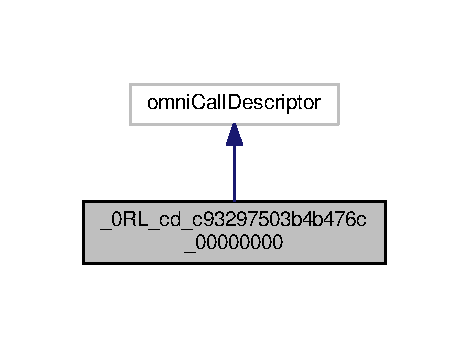
\includegraphics[width=225pt]{class__0_r_l__cd__c93297503b4b476c__00000000__coll__graph}
\end{center}
\end{figure}
\subsection*{Public Member Functions}
\begin{DoxyCompactItemize}
\item 
\hyperlink{class__0_r_l__cd__c93297503b4b476c__00000000_a39fa42d3fde3b25c87627f66cae0ea88}{\+\_\+0\+R\+L\+\_\+cd\+\_\+c93297503b4b476c\+\_\+00000000} (Local\+Call\+Fn lcfn, const char $\ast$op\+\_\+, size\+\_\+t oplen, \+\_\+\+C\+O\+R\+B\+A\+\_\+\+Boolean upcall=0)
\item 
void \hyperlink{class__0_r_l__cd__c93297503b4b476c__00000000_a30a9ce428cfc2b4e1bed20f2aea500d5}{marshal\+Arguments} (cdr\+Stream \&)
\item 
void \hyperlink{class__0_r_l__cd__c93297503b4b476c__00000000_a62c797ae6a2627ed0b0ec4c8775ef15b}{unmarshal\+Arguments} (cdr\+Stream \&)
\item 
void \hyperlink{class__0_r_l__cd__c93297503b4b476c__00000000_a8f8e55e3b23e45bd169848018d148c2e}{unmarshal\+Returned\+Values} (cdr\+Stream \&)
\item 
void \hyperlink{class__0_r_l__cd__c93297503b4b476c__00000000_ad3be4ef51381ee2c0069772e59b2f99a}{marshal\+Returned\+Values} (cdr\+Stream \&)
\item 
void \hyperlink{class__0_r_l__cd__c93297503b4b476c__00000000_a3b5d41f45aa39c10bcce7877f5b45e8b}{user\+Exception} (cdr\+Stream \&, \+\_\+\+O\+M\+N\+I\+\_\+\+NS(I\+O\+P\+\_\+C)$\ast$, const char $\ast$)
\end{DoxyCompactItemize}
\subsection*{Public Attributes}
\begin{DoxyCompactItemize}
\item 
\+::C\+O\+R\+B\+A\+::\+Long \hyperlink{class__0_r_l__cd__c93297503b4b476c__00000000_a9d70bde12d4e7bf6319ad0d2bd20a813}{arg\+\_\+0}
\item 
\+::C\+O\+R\+B\+A\+::\+Double \hyperlink{class__0_r_l__cd__c93297503b4b476c__00000000_a1f600d809c6391de305682594e9b03f7}{result}
\end{DoxyCompactItemize}
\subsection*{Static Public Attributes}
\begin{DoxyCompactItemize}
\item 
static const char $\ast$const \hyperlink{class__0_r_l__cd__c93297503b4b476c__00000000_aed815b8e10305526569276393b2f0675}{\+\_\+user\+\_\+exns} \mbox{[}$\,$\mbox{]}
\end{DoxyCompactItemize}


\subsection{Constructor \& Destructor Documentation}
\index{\+\_\+0\+R\+L\+\_\+cd\+\_\+c93297503b4b476c\+\_\+00000000@{\+\_\+0\+R\+L\+\_\+cd\+\_\+c93297503b4b476c\+\_\+00000000}!\+\_\+0\+R\+L\+\_\+cd\+\_\+c93297503b4b476c\+\_\+00000000@{\+\_\+0\+R\+L\+\_\+cd\+\_\+c93297503b4b476c\+\_\+00000000}}
\index{\+\_\+0\+R\+L\+\_\+cd\+\_\+c93297503b4b476c\+\_\+00000000@{\+\_\+0\+R\+L\+\_\+cd\+\_\+c93297503b4b476c\+\_\+00000000}!\+\_\+0\+R\+L\+\_\+cd\+\_\+c93297503b4b476c\+\_\+00000000@{\+\_\+0\+R\+L\+\_\+cd\+\_\+c93297503b4b476c\+\_\+00000000}}
\subsubsection[{\texorpdfstring{\+\_\+0\+R\+L\+\_\+cd\+\_\+c93297503b4b476c\+\_\+00000000(\+Local\+Call\+Fn lcfn, const char $\ast$op\+\_\+, size\+\_\+t oplen, \+\_\+\+C\+O\+R\+B\+A\+\_\+\+Boolean upcall=0)}{_0RL_cd_c93297503b4b476c_00000000(LocalCallFn lcfn, const char *op_, size_t oplen, _CORBA_Boolean upcall=0)}}]{\setlength{\rightskip}{0pt plus 5cm}\+\_\+0\+R\+L\+\_\+cd\+\_\+c93297503b4b476c\+\_\+00000000\+::\+\_\+0\+R\+L\+\_\+cd\+\_\+c93297503b4b476c\+\_\+00000000 (
\begin{DoxyParamCaption}
\item[{Local\+Call\+Fn}]{lcfn, }
\item[{const char $\ast$}]{op\+\_\+, }
\item[{size\+\_\+t}]{oplen, }
\item[{\+\_\+\+C\+O\+R\+B\+A\+\_\+\+Boolean}]{upcall = {\ttfamily 0}}
\end{DoxyParamCaption}
)\hspace{0.3cm}{\ttfamily [inline]}}\hypertarget{class__0_r_l__cd__c93297503b4b476c__00000000_a39fa42d3fde3b25c87627f66cae0ea88}{}\label{class__0_r_l__cd__c93297503b4b476c__00000000_a39fa42d3fde3b25c87627f66cae0ea88}


\subsection{Member Function Documentation}
\index{\+\_\+0\+R\+L\+\_\+cd\+\_\+c93297503b4b476c\+\_\+00000000@{\+\_\+0\+R\+L\+\_\+cd\+\_\+c93297503b4b476c\+\_\+00000000}!marshal\+Arguments@{marshal\+Arguments}}
\index{marshal\+Arguments@{marshal\+Arguments}!\+\_\+0\+R\+L\+\_\+cd\+\_\+c93297503b4b476c\+\_\+00000000@{\+\_\+0\+R\+L\+\_\+cd\+\_\+c93297503b4b476c\+\_\+00000000}}
\subsubsection[{\texorpdfstring{marshal\+Arguments(cdr\+Stream \&)}{marshalArguments(cdrStream &)}}]{\setlength{\rightskip}{0pt plus 5cm}void \+\_\+0\+R\+L\+\_\+cd\+\_\+c93297503b4b476c\+\_\+00000000\+::marshal\+Arguments (
\begin{DoxyParamCaption}
\item[{cdr\+Stream \&}]{\+\_\+n}
\end{DoxyParamCaption}
)}\hypertarget{class__0_r_l__cd__c93297503b4b476c__00000000_a30a9ce428cfc2b4e1bed20f2aea500d5}{}\label{class__0_r_l__cd__c93297503b4b476c__00000000_a30a9ce428cfc2b4e1bed20f2aea500d5}
\index{\+\_\+0\+R\+L\+\_\+cd\+\_\+c93297503b4b476c\+\_\+00000000@{\+\_\+0\+R\+L\+\_\+cd\+\_\+c93297503b4b476c\+\_\+00000000}!marshal\+Returned\+Values@{marshal\+Returned\+Values}}
\index{marshal\+Returned\+Values@{marshal\+Returned\+Values}!\+\_\+0\+R\+L\+\_\+cd\+\_\+c93297503b4b476c\+\_\+00000000@{\+\_\+0\+R\+L\+\_\+cd\+\_\+c93297503b4b476c\+\_\+00000000}}
\subsubsection[{\texorpdfstring{marshal\+Returned\+Values(cdr\+Stream \&)}{marshalReturnedValues(cdrStream &)}}]{\setlength{\rightskip}{0pt plus 5cm}void \+\_\+0\+R\+L\+\_\+cd\+\_\+c93297503b4b476c\+\_\+00000000\+::marshal\+Returned\+Values (
\begin{DoxyParamCaption}
\item[{cdr\+Stream \&}]{\+\_\+n}
\end{DoxyParamCaption}
)}\hypertarget{class__0_r_l__cd__c93297503b4b476c__00000000_ad3be4ef51381ee2c0069772e59b2f99a}{}\label{class__0_r_l__cd__c93297503b4b476c__00000000_ad3be4ef51381ee2c0069772e59b2f99a}
\index{\+\_\+0\+R\+L\+\_\+cd\+\_\+c93297503b4b476c\+\_\+00000000@{\+\_\+0\+R\+L\+\_\+cd\+\_\+c93297503b4b476c\+\_\+00000000}!unmarshal\+Arguments@{unmarshal\+Arguments}}
\index{unmarshal\+Arguments@{unmarshal\+Arguments}!\+\_\+0\+R\+L\+\_\+cd\+\_\+c93297503b4b476c\+\_\+00000000@{\+\_\+0\+R\+L\+\_\+cd\+\_\+c93297503b4b476c\+\_\+00000000}}
\subsubsection[{\texorpdfstring{unmarshal\+Arguments(cdr\+Stream \&)}{unmarshalArguments(cdrStream &)}}]{\setlength{\rightskip}{0pt plus 5cm}void \+\_\+0\+R\+L\+\_\+cd\+\_\+c93297503b4b476c\+\_\+00000000\+::unmarshal\+Arguments (
\begin{DoxyParamCaption}
\item[{cdr\+Stream \&}]{\+\_\+n}
\end{DoxyParamCaption}
)}\hypertarget{class__0_r_l__cd__c93297503b4b476c__00000000_a62c797ae6a2627ed0b0ec4c8775ef15b}{}\label{class__0_r_l__cd__c93297503b4b476c__00000000_a62c797ae6a2627ed0b0ec4c8775ef15b}
\index{\+\_\+0\+R\+L\+\_\+cd\+\_\+c93297503b4b476c\+\_\+00000000@{\+\_\+0\+R\+L\+\_\+cd\+\_\+c93297503b4b476c\+\_\+00000000}!unmarshal\+Returned\+Values@{unmarshal\+Returned\+Values}}
\index{unmarshal\+Returned\+Values@{unmarshal\+Returned\+Values}!\+\_\+0\+R\+L\+\_\+cd\+\_\+c93297503b4b476c\+\_\+00000000@{\+\_\+0\+R\+L\+\_\+cd\+\_\+c93297503b4b476c\+\_\+00000000}}
\subsubsection[{\texorpdfstring{unmarshal\+Returned\+Values(cdr\+Stream \&)}{unmarshalReturnedValues(cdrStream &)}}]{\setlength{\rightskip}{0pt plus 5cm}void \+\_\+0\+R\+L\+\_\+cd\+\_\+c93297503b4b476c\+\_\+00000000\+::unmarshal\+Returned\+Values (
\begin{DoxyParamCaption}
\item[{cdr\+Stream \&}]{\+\_\+n}
\end{DoxyParamCaption}
)}\hypertarget{class__0_r_l__cd__c93297503b4b476c__00000000_a8f8e55e3b23e45bd169848018d148c2e}{}\label{class__0_r_l__cd__c93297503b4b476c__00000000_a8f8e55e3b23e45bd169848018d148c2e}
\index{\+\_\+0\+R\+L\+\_\+cd\+\_\+c93297503b4b476c\+\_\+00000000@{\+\_\+0\+R\+L\+\_\+cd\+\_\+c93297503b4b476c\+\_\+00000000}!user\+Exception@{user\+Exception}}
\index{user\+Exception@{user\+Exception}!\+\_\+0\+R\+L\+\_\+cd\+\_\+c93297503b4b476c\+\_\+00000000@{\+\_\+0\+R\+L\+\_\+cd\+\_\+c93297503b4b476c\+\_\+00000000}}
\subsubsection[{\texorpdfstring{user\+Exception(cdr\+Stream \&, \+\_\+\+O\+M\+N\+I\+\_\+\+N\+S(\+I\+O\+P\+\_\+\+C)$\ast$, const char $\ast$)}{userException(cdrStream &, _OMNI_NS(IOP_C)*, const char *)}}]{\setlength{\rightskip}{0pt plus 5cm}void \+\_\+0\+R\+L\+\_\+cd\+\_\+c93297503b4b476c\+\_\+00000000\+::user\+Exception (
\begin{DoxyParamCaption}
\item[{cdr\+Stream \&}]{s, }
\item[{\+\_\+\+O\+M\+N\+I\+\_\+\+NS(I\+O\+P\+\_\+C)$\ast$}]{iop\+\_\+client, }
\item[{const char $\ast$}]{repo\+Id}
\end{DoxyParamCaption}
)}\hypertarget{class__0_r_l__cd__c93297503b4b476c__00000000_a3b5d41f45aa39c10bcce7877f5b45e8b}{}\label{class__0_r_l__cd__c93297503b4b476c__00000000_a3b5d41f45aa39c10bcce7877f5b45e8b}


\subsection{Member Data Documentation}
\index{\+\_\+0\+R\+L\+\_\+cd\+\_\+c93297503b4b476c\+\_\+00000000@{\+\_\+0\+R\+L\+\_\+cd\+\_\+c93297503b4b476c\+\_\+00000000}!\+\_\+user\+\_\+exns@{\+\_\+user\+\_\+exns}}
\index{\+\_\+user\+\_\+exns@{\+\_\+user\+\_\+exns}!\+\_\+0\+R\+L\+\_\+cd\+\_\+c93297503b4b476c\+\_\+00000000@{\+\_\+0\+R\+L\+\_\+cd\+\_\+c93297503b4b476c\+\_\+00000000}}
\subsubsection[{\texorpdfstring{\+\_\+user\+\_\+exns}{_user_exns}}]{\setlength{\rightskip}{0pt plus 5cm}const char $\ast$const \+\_\+0\+R\+L\+\_\+cd\+\_\+c93297503b4b476c\+\_\+00000000\+::\+\_\+user\+\_\+exns\hspace{0.3cm}{\ttfamily [static]}}\hypertarget{class__0_r_l__cd__c93297503b4b476c__00000000_aed815b8e10305526569276393b2f0675}{}\label{class__0_r_l__cd__c93297503b4b476c__00000000_aed815b8e10305526569276393b2f0675}
{\bfseries Initial value\+:}
\begin{DoxyCode}
= \{
  PetitPrince::DrawService::NonApplicable::\_PD\_repoId
\}
\end{DoxyCode}
\index{\+\_\+0\+R\+L\+\_\+cd\+\_\+c93297503b4b476c\+\_\+00000000@{\+\_\+0\+R\+L\+\_\+cd\+\_\+c93297503b4b476c\+\_\+00000000}!arg\+\_\+0@{arg\+\_\+0}}
\index{arg\+\_\+0@{arg\+\_\+0}!\+\_\+0\+R\+L\+\_\+cd\+\_\+c93297503b4b476c\+\_\+00000000@{\+\_\+0\+R\+L\+\_\+cd\+\_\+c93297503b4b476c\+\_\+00000000}}
\subsubsection[{\texorpdfstring{arg\+\_\+0}{arg_0}}]{\setlength{\rightskip}{0pt plus 5cm}\+::C\+O\+R\+B\+A\+::\+Long \+\_\+0\+R\+L\+\_\+cd\+\_\+c93297503b4b476c\+\_\+00000000\+::arg\+\_\+0}\hypertarget{class__0_r_l__cd__c93297503b4b476c__00000000_a9d70bde12d4e7bf6319ad0d2bd20a813}{}\label{class__0_r_l__cd__c93297503b4b476c__00000000_a9d70bde12d4e7bf6319ad0d2bd20a813}
\index{\+\_\+0\+R\+L\+\_\+cd\+\_\+c93297503b4b476c\+\_\+00000000@{\+\_\+0\+R\+L\+\_\+cd\+\_\+c93297503b4b476c\+\_\+00000000}!result@{result}}
\index{result@{result}!\+\_\+0\+R\+L\+\_\+cd\+\_\+c93297503b4b476c\+\_\+00000000@{\+\_\+0\+R\+L\+\_\+cd\+\_\+c93297503b4b476c\+\_\+00000000}}
\subsubsection[{\texorpdfstring{result}{result}}]{\setlength{\rightskip}{0pt plus 5cm}\+::C\+O\+R\+B\+A\+::\+Double \+\_\+0\+R\+L\+\_\+cd\+\_\+c93297503b4b476c\+\_\+00000000\+::result}\hypertarget{class__0_r_l__cd__c93297503b4b476c__00000000_a1f600d809c6391de305682594e9b03f7}{}\label{class__0_r_l__cd__c93297503b4b476c__00000000_a1f600d809c6391de305682594e9b03f7}


The documentation for this class was generated from the following file\+:\begin{DoxyCompactItemize}
\item 
src/\hyperlink{_petit_prince___stub_8cpp}{Petit\+Prince\+\_\+\+Stub.\+cpp}\end{DoxyCompactItemize}

\hypertarget{class__0_r_l__cd__c93297503b4b476c__11000000}{}\section{\+\_\+0\+R\+L\+\_\+cd\+\_\+c93297503b4b476c\+\_\+11000000 Class Reference}
\label{class__0_r_l__cd__c93297503b4b476c__11000000}\index{\+\_\+0\+R\+L\+\_\+cd\+\_\+c93297503b4b476c\+\_\+11000000@{\+\_\+0\+R\+L\+\_\+cd\+\_\+c93297503b4b476c\+\_\+11000000}}


Inheritance diagram for \+\_\+0\+R\+L\+\_\+cd\+\_\+c93297503b4b476c\+\_\+11000000\+:
\nopagebreak
\begin{figure}[H]
\begin{center}
\leavevmode
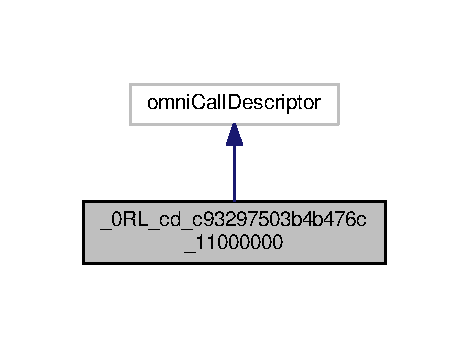
\includegraphics[width=225pt]{class__0_r_l__cd__c93297503b4b476c__11000000__inherit__graph}
\end{center}
\end{figure}


Collaboration diagram for \+\_\+0\+R\+L\+\_\+cd\+\_\+c93297503b4b476c\+\_\+11000000\+:
\nopagebreak
\begin{figure}[H]
\begin{center}
\leavevmode
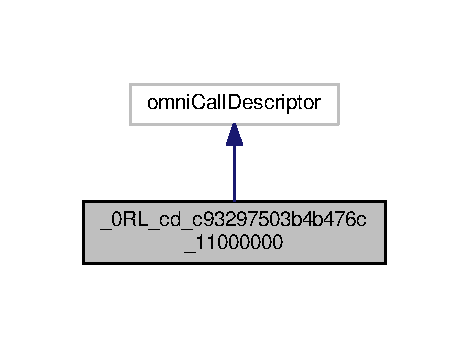
\includegraphics[width=225pt]{class__0_r_l__cd__c93297503b4b476c__11000000__coll__graph}
\end{center}
\end{figure}
\subsection*{Public Member Functions}
\begin{DoxyCompactItemize}
\item 
\hyperlink{class__0_r_l__cd__c93297503b4b476c__11000000_a1bb4893a79836d1d8bc3b28b56a7938a}{\+\_\+0\+R\+L\+\_\+cd\+\_\+c93297503b4b476c\+\_\+11000000} (Local\+Call\+Fn lcfn, const char $\ast$op\+\_\+, size\+\_\+t oplen, \+\_\+\+C\+O\+R\+B\+A\+\_\+\+Boolean upcall=0)
\item 
void \hyperlink{class__0_r_l__cd__c93297503b4b476c__11000000_a49560150918cbb146c8da79944df19c9}{marshal\+Arguments} (cdr\+Stream \&)
\item 
void \hyperlink{class__0_r_l__cd__c93297503b4b476c__11000000_abe687c880ef4f26e6b4001adfd828a07}{unmarshal\+Arguments} (cdr\+Stream \&)
\item 
void \hyperlink{class__0_r_l__cd__c93297503b4b476c__11000000_a053ad3b798898324014ca65e3e96920d}{unmarshal\+Returned\+Values} (cdr\+Stream \&)
\item 
void \hyperlink{class__0_r_l__cd__c93297503b4b476c__11000000_a5b1e30673b954c10405a8a652324088f}{marshal\+Returned\+Values} (cdr\+Stream \&)
\item 
void \hyperlink{class__0_r_l__cd__c93297503b4b476c__11000000_a8a923df033dc3177185f90d879451022}{user\+Exception} (cdr\+Stream \&, \+\_\+\+O\+M\+N\+I\+\_\+\+NS(I\+O\+P\+\_\+C)$\ast$, const char $\ast$)
\end{DoxyCompactItemize}
\subsection*{Public Attributes}
\begin{DoxyCompactItemize}
\item 
\+::C\+O\+R\+B\+A\+::\+String\+\_\+var \hyperlink{class__0_r_l__cd__c93297503b4b476c__11000000_abdc0a1fecfa33dd766c72760623a2bb0}{arg\+\_\+0\+\_\+}
\item 
const char $\ast$ \hyperlink{class__0_r_l__cd__c93297503b4b476c__11000000_a028225d9a02bc49290dc044801396b57}{arg\+\_\+0}
\item 
Petit\+Prince\+::\+Point \hyperlink{class__0_r_l__cd__c93297503b4b476c__11000000_a36cb208c9c1152cddc301d382e4fec23}{arg\+\_\+1\+\_\+}
\item 
const Petit\+Prince\+::\+Point $\ast$ \hyperlink{class__0_r_l__cd__c93297503b4b476c__11000000_ab3cb660dcca4e79904955484dce2b56e}{arg\+\_\+1}
\item 
\+::C\+O\+R\+B\+A\+::\+Double \hyperlink{class__0_r_l__cd__c93297503b4b476c__11000000_a67084e7fa5c434110e588481b53a61c2}{arg\+\_\+2}
\item 
\+::C\+O\+R\+B\+A\+::\+Long \hyperlink{class__0_r_l__cd__c93297503b4b476c__11000000_a5e87affab2cb58f2a874bb8572df0486}{result}
\end{DoxyCompactItemize}
\subsection*{Static Public Attributes}
\begin{DoxyCompactItemize}
\item 
static const char $\ast$const \hyperlink{class__0_r_l__cd__c93297503b4b476c__11000000_a538cdbcd31ccae802ef65d3faebeac42}{\+\_\+user\+\_\+exns} \mbox{[}$\,$\mbox{]}
\end{DoxyCompactItemize}


\subsection{Detailed Description}


Definition at line 2017 of file Petit\+Prince\+\_\+\+Stub.\+cpp.



\subsection{Constructor \& Destructor Documentation}
\index{\+\_\+0\+R\+L\+\_\+cd\+\_\+c93297503b4b476c\+\_\+11000000@{\+\_\+0\+R\+L\+\_\+cd\+\_\+c93297503b4b476c\+\_\+11000000}!\+\_\+0\+R\+L\+\_\+cd\+\_\+c93297503b4b476c\+\_\+11000000@{\+\_\+0\+R\+L\+\_\+cd\+\_\+c93297503b4b476c\+\_\+11000000}}
\index{\+\_\+0\+R\+L\+\_\+cd\+\_\+c93297503b4b476c\+\_\+11000000@{\+\_\+0\+R\+L\+\_\+cd\+\_\+c93297503b4b476c\+\_\+11000000}!\+\_\+0\+R\+L\+\_\+cd\+\_\+c93297503b4b476c\+\_\+11000000@{\+\_\+0\+R\+L\+\_\+cd\+\_\+c93297503b4b476c\+\_\+11000000}}
\subsubsection[{\texorpdfstring{\+\_\+0\+R\+L\+\_\+cd\+\_\+c93297503b4b476c\+\_\+11000000(\+Local\+Call\+Fn lcfn, const char $\ast$op\+\_\+, size\+\_\+t oplen, \+\_\+\+C\+O\+R\+B\+A\+\_\+\+Boolean upcall=0)}{_0RL_cd_c93297503b4b476c_11000000(LocalCallFn lcfn, const char *op_, size_t oplen, _CORBA_Boolean upcall=0)}}]{\setlength{\rightskip}{0pt plus 5cm}\+\_\+0\+R\+L\+\_\+cd\+\_\+c93297503b4b476c\+\_\+11000000\+::\+\_\+0\+R\+L\+\_\+cd\+\_\+c93297503b4b476c\+\_\+11000000 (
\begin{DoxyParamCaption}
\item[{Local\+Call\+Fn}]{lcfn, }
\item[{const char $\ast$}]{op\+\_\+, }
\item[{size\+\_\+t}]{oplen, }
\item[{\+\_\+\+C\+O\+R\+B\+A\+\_\+\+Boolean}]{upcall = {\ttfamily 0}}
\end{DoxyParamCaption}
)\hspace{0.3cm}{\ttfamily [inline]}}\hypertarget{class__0_r_l__cd__c93297503b4b476c__11000000_a1bb4893a79836d1d8bc3b28b56a7938a}{}\label{class__0_r_l__cd__c93297503b4b476c__11000000_a1bb4893a79836d1d8bc3b28b56a7938a}


Definition at line 2021 of file Petit\+Prince\+\_\+\+Stub.\+cpp.



\subsection{Member Function Documentation}
\index{\+\_\+0\+R\+L\+\_\+cd\+\_\+c93297503b4b476c\+\_\+11000000@{\+\_\+0\+R\+L\+\_\+cd\+\_\+c93297503b4b476c\+\_\+11000000}!marshal\+Arguments@{marshal\+Arguments}}
\index{marshal\+Arguments@{marshal\+Arguments}!\+\_\+0\+R\+L\+\_\+cd\+\_\+c93297503b4b476c\+\_\+11000000@{\+\_\+0\+R\+L\+\_\+cd\+\_\+c93297503b4b476c\+\_\+11000000}}
\subsubsection[{\texorpdfstring{marshal\+Arguments(cdr\+Stream \&)}{marshalArguments(cdrStream &)}}]{\setlength{\rightskip}{0pt plus 5cm}void \+\_\+0\+R\+L\+\_\+cd\+\_\+c93297503b4b476c\+\_\+11000000\+::marshal\+Arguments (
\begin{DoxyParamCaption}
\item[{cdr\+Stream \&}]{\+\_\+n}
\end{DoxyParamCaption}
)}\hypertarget{class__0_r_l__cd__c93297503b4b476c__11000000_a49560150918cbb146c8da79944df19c9}{}\label{class__0_r_l__cd__c93297503b4b476c__11000000_a49560150918cbb146c8da79944df19c9}


Definition at line 2044 of file Petit\+Prince\+\_\+\+Stub.\+cpp.

\index{\+\_\+0\+R\+L\+\_\+cd\+\_\+c93297503b4b476c\+\_\+11000000@{\+\_\+0\+R\+L\+\_\+cd\+\_\+c93297503b4b476c\+\_\+11000000}!marshal\+Returned\+Values@{marshal\+Returned\+Values}}
\index{marshal\+Returned\+Values@{marshal\+Returned\+Values}!\+\_\+0\+R\+L\+\_\+cd\+\_\+c93297503b4b476c\+\_\+11000000@{\+\_\+0\+R\+L\+\_\+cd\+\_\+c93297503b4b476c\+\_\+11000000}}
\subsubsection[{\texorpdfstring{marshal\+Returned\+Values(cdr\+Stream \&)}{marshalReturnedValues(cdrStream &)}}]{\setlength{\rightskip}{0pt plus 5cm}void \+\_\+0\+R\+L\+\_\+cd\+\_\+c93297503b4b476c\+\_\+11000000\+::marshal\+Returned\+Values (
\begin{DoxyParamCaption}
\item[{cdr\+Stream \&}]{\+\_\+n}
\end{DoxyParamCaption}
)}\hypertarget{class__0_r_l__cd__c93297503b4b476c__11000000_a5b1e30673b954c10405a8a652324088f}{}\label{class__0_r_l__cd__c93297503b4b476c__11000000_a5b1e30673b954c10405a8a652324088f}


Definition at line 2062 of file Petit\+Prince\+\_\+\+Stub.\+cpp.

\index{\+\_\+0\+R\+L\+\_\+cd\+\_\+c93297503b4b476c\+\_\+11000000@{\+\_\+0\+R\+L\+\_\+cd\+\_\+c93297503b4b476c\+\_\+11000000}!unmarshal\+Arguments@{unmarshal\+Arguments}}
\index{unmarshal\+Arguments@{unmarshal\+Arguments}!\+\_\+0\+R\+L\+\_\+cd\+\_\+c93297503b4b476c\+\_\+11000000@{\+\_\+0\+R\+L\+\_\+cd\+\_\+c93297503b4b476c\+\_\+11000000}}
\subsubsection[{\texorpdfstring{unmarshal\+Arguments(cdr\+Stream \&)}{unmarshalArguments(cdrStream &)}}]{\setlength{\rightskip}{0pt plus 5cm}void \+\_\+0\+R\+L\+\_\+cd\+\_\+c93297503b4b476c\+\_\+11000000\+::unmarshal\+Arguments (
\begin{DoxyParamCaption}
\item[{cdr\+Stream \&}]{\+\_\+n}
\end{DoxyParamCaption}
)}\hypertarget{class__0_r_l__cd__c93297503b4b476c__11000000_abe687c880ef4f26e6b4001adfd828a07}{}\label{class__0_r_l__cd__c93297503b4b476c__11000000_abe687c880ef4f26e6b4001adfd828a07}


Definition at line 2052 of file Petit\+Prince\+\_\+\+Stub.\+cpp.

\index{\+\_\+0\+R\+L\+\_\+cd\+\_\+c93297503b4b476c\+\_\+11000000@{\+\_\+0\+R\+L\+\_\+cd\+\_\+c93297503b4b476c\+\_\+11000000}!unmarshal\+Returned\+Values@{unmarshal\+Returned\+Values}}
\index{unmarshal\+Returned\+Values@{unmarshal\+Returned\+Values}!\+\_\+0\+R\+L\+\_\+cd\+\_\+c93297503b4b476c\+\_\+11000000@{\+\_\+0\+R\+L\+\_\+cd\+\_\+c93297503b4b476c\+\_\+11000000}}
\subsubsection[{\texorpdfstring{unmarshal\+Returned\+Values(cdr\+Stream \&)}{unmarshalReturnedValues(cdrStream &)}}]{\setlength{\rightskip}{0pt plus 5cm}void \+\_\+0\+R\+L\+\_\+cd\+\_\+c93297503b4b476c\+\_\+11000000\+::unmarshal\+Returned\+Values (
\begin{DoxyParamCaption}
\item[{cdr\+Stream \&}]{\+\_\+n}
\end{DoxyParamCaption}
)}\hypertarget{class__0_r_l__cd__c93297503b4b476c__11000000_a053ad3b798898324014ca65e3e96920d}{}\label{class__0_r_l__cd__c93297503b4b476c__11000000_a053ad3b798898324014ca65e3e96920d}


Definition at line 2068 of file Petit\+Prince\+\_\+\+Stub.\+cpp.

\index{\+\_\+0\+R\+L\+\_\+cd\+\_\+c93297503b4b476c\+\_\+11000000@{\+\_\+0\+R\+L\+\_\+cd\+\_\+c93297503b4b476c\+\_\+11000000}!user\+Exception@{user\+Exception}}
\index{user\+Exception@{user\+Exception}!\+\_\+0\+R\+L\+\_\+cd\+\_\+c93297503b4b476c\+\_\+11000000@{\+\_\+0\+R\+L\+\_\+cd\+\_\+c93297503b4b476c\+\_\+11000000}}
\subsubsection[{\texorpdfstring{user\+Exception(cdr\+Stream \&, \+\_\+\+O\+M\+N\+I\+\_\+\+N\+S(\+I\+O\+P\+\_\+\+C)$\ast$, const char $\ast$)}{userException(cdrStream &, _OMNI_NS(IOP_C)*, const char *)}}]{\setlength{\rightskip}{0pt plus 5cm}void \+\_\+0\+R\+L\+\_\+cd\+\_\+c93297503b4b476c\+\_\+11000000\+::user\+Exception (
\begin{DoxyParamCaption}
\item[{cdr\+Stream \&}]{s, }
\item[{\+\_\+\+O\+M\+N\+I\+\_\+\+NS(I\+O\+P\+\_\+C)$\ast$}]{iop\+\_\+client, }
\item[{const char $\ast$}]{repo\+Id}
\end{DoxyParamCaption}
)}\hypertarget{class__0_r_l__cd__c93297503b4b476c__11000000_a8a923df033dc3177185f90d879451022}{}\label{class__0_r_l__cd__c93297503b4b476c__11000000_a8a923df033dc3177185f90d879451022}


Definition at line 2078 of file Petit\+Prince\+\_\+\+Stub.\+cpp.



\subsection{Member Data Documentation}
\index{\+\_\+0\+R\+L\+\_\+cd\+\_\+c93297503b4b476c\+\_\+11000000@{\+\_\+0\+R\+L\+\_\+cd\+\_\+c93297503b4b476c\+\_\+11000000}!\+\_\+user\+\_\+exns@{\+\_\+user\+\_\+exns}}
\index{\+\_\+user\+\_\+exns@{\+\_\+user\+\_\+exns}!\+\_\+0\+R\+L\+\_\+cd\+\_\+c93297503b4b476c\+\_\+11000000@{\+\_\+0\+R\+L\+\_\+cd\+\_\+c93297503b4b476c\+\_\+11000000}}
\subsubsection[{\texorpdfstring{\+\_\+user\+\_\+exns}{_user_exns}}]{\setlength{\rightskip}{0pt plus 5cm}const char $\ast$const \+\_\+0\+R\+L\+\_\+cd\+\_\+c93297503b4b476c\+\_\+11000000\+::\+\_\+user\+\_\+exns\hspace{0.3cm}{\ttfamily [static]}}\hypertarget{class__0_r_l__cd__c93297503b4b476c__11000000_a538cdbcd31ccae802ef65d3faebeac42}{}\label{class__0_r_l__cd__c93297503b4b476c__11000000_a538cdbcd31ccae802ef65d3faebeac42}
{\bfseries Initial value\+:}
\begin{DoxyCode}
= \{
  PetitPrince::PetitPrinceService::InvalidDrawParams::\_PD\_repoId
\}
\end{DoxyCode}


Definition at line 2034 of file Petit\+Prince\+\_\+\+Stub.\+cpp.

\index{\+\_\+0\+R\+L\+\_\+cd\+\_\+c93297503b4b476c\+\_\+11000000@{\+\_\+0\+R\+L\+\_\+cd\+\_\+c93297503b4b476c\+\_\+11000000}!arg\+\_\+0@{arg\+\_\+0}}
\index{arg\+\_\+0@{arg\+\_\+0}!\+\_\+0\+R\+L\+\_\+cd\+\_\+c93297503b4b476c\+\_\+11000000@{\+\_\+0\+R\+L\+\_\+cd\+\_\+c93297503b4b476c\+\_\+11000000}}
\subsubsection[{\texorpdfstring{arg\+\_\+0}{arg_0}}]{\setlength{\rightskip}{0pt plus 5cm}const char$\ast$ \+\_\+0\+R\+L\+\_\+cd\+\_\+c93297503b4b476c\+\_\+11000000\+::arg\+\_\+0}\hypertarget{class__0_r_l__cd__c93297503b4b476c__11000000_a028225d9a02bc49290dc044801396b57}{}\label{class__0_r_l__cd__c93297503b4b476c__11000000_a028225d9a02bc49290dc044801396b57}


Definition at line 2037 of file Petit\+Prince\+\_\+\+Stub.\+cpp.

\index{\+\_\+0\+R\+L\+\_\+cd\+\_\+c93297503b4b476c\+\_\+11000000@{\+\_\+0\+R\+L\+\_\+cd\+\_\+c93297503b4b476c\+\_\+11000000}!arg\+\_\+0\+\_\+@{arg\+\_\+0\+\_\+}}
\index{arg\+\_\+0\+\_\+@{arg\+\_\+0\+\_\+}!\+\_\+0\+R\+L\+\_\+cd\+\_\+c93297503b4b476c\+\_\+11000000@{\+\_\+0\+R\+L\+\_\+cd\+\_\+c93297503b4b476c\+\_\+11000000}}
\subsubsection[{\texorpdfstring{arg\+\_\+0\+\_\+}{arg_0_}}]{\setlength{\rightskip}{0pt plus 5cm}\+::C\+O\+R\+B\+A\+::\+String\+\_\+var \+\_\+0\+R\+L\+\_\+cd\+\_\+c93297503b4b476c\+\_\+11000000\+::arg\+\_\+0\+\_\+}\hypertarget{class__0_r_l__cd__c93297503b4b476c__11000000_abdc0a1fecfa33dd766c72760623a2bb0}{}\label{class__0_r_l__cd__c93297503b4b476c__11000000_abdc0a1fecfa33dd766c72760623a2bb0}


Definition at line 2036 of file Petit\+Prince\+\_\+\+Stub.\+cpp.

\index{\+\_\+0\+R\+L\+\_\+cd\+\_\+c93297503b4b476c\+\_\+11000000@{\+\_\+0\+R\+L\+\_\+cd\+\_\+c93297503b4b476c\+\_\+11000000}!arg\+\_\+1@{arg\+\_\+1}}
\index{arg\+\_\+1@{arg\+\_\+1}!\+\_\+0\+R\+L\+\_\+cd\+\_\+c93297503b4b476c\+\_\+11000000@{\+\_\+0\+R\+L\+\_\+cd\+\_\+c93297503b4b476c\+\_\+11000000}}
\subsubsection[{\texorpdfstring{arg\+\_\+1}{arg_1}}]{\setlength{\rightskip}{0pt plus 5cm}const Petit\+Prince\+::\+Point$\ast$ \+\_\+0\+R\+L\+\_\+cd\+\_\+c93297503b4b476c\+\_\+11000000\+::arg\+\_\+1}\hypertarget{class__0_r_l__cd__c93297503b4b476c__11000000_ab3cb660dcca4e79904955484dce2b56e}{}\label{class__0_r_l__cd__c93297503b4b476c__11000000_ab3cb660dcca4e79904955484dce2b56e}


Definition at line 2039 of file Petit\+Prince\+\_\+\+Stub.\+cpp.

\index{\+\_\+0\+R\+L\+\_\+cd\+\_\+c93297503b4b476c\+\_\+11000000@{\+\_\+0\+R\+L\+\_\+cd\+\_\+c93297503b4b476c\+\_\+11000000}!arg\+\_\+1\+\_\+@{arg\+\_\+1\+\_\+}}
\index{arg\+\_\+1\+\_\+@{arg\+\_\+1\+\_\+}!\+\_\+0\+R\+L\+\_\+cd\+\_\+c93297503b4b476c\+\_\+11000000@{\+\_\+0\+R\+L\+\_\+cd\+\_\+c93297503b4b476c\+\_\+11000000}}
\subsubsection[{\texorpdfstring{arg\+\_\+1\+\_\+}{arg_1_}}]{\setlength{\rightskip}{0pt plus 5cm}Petit\+Prince\+::\+Point \+\_\+0\+R\+L\+\_\+cd\+\_\+c93297503b4b476c\+\_\+11000000\+::arg\+\_\+1\+\_\+}\hypertarget{class__0_r_l__cd__c93297503b4b476c__11000000_a36cb208c9c1152cddc301d382e4fec23}{}\label{class__0_r_l__cd__c93297503b4b476c__11000000_a36cb208c9c1152cddc301d382e4fec23}


Definition at line 2038 of file Petit\+Prince\+\_\+\+Stub.\+cpp.

\index{\+\_\+0\+R\+L\+\_\+cd\+\_\+c93297503b4b476c\+\_\+11000000@{\+\_\+0\+R\+L\+\_\+cd\+\_\+c93297503b4b476c\+\_\+11000000}!arg\+\_\+2@{arg\+\_\+2}}
\index{arg\+\_\+2@{arg\+\_\+2}!\+\_\+0\+R\+L\+\_\+cd\+\_\+c93297503b4b476c\+\_\+11000000@{\+\_\+0\+R\+L\+\_\+cd\+\_\+c93297503b4b476c\+\_\+11000000}}
\subsubsection[{\texorpdfstring{arg\+\_\+2}{arg_2}}]{\setlength{\rightskip}{0pt plus 5cm}\+::C\+O\+R\+B\+A\+::\+Double \+\_\+0\+R\+L\+\_\+cd\+\_\+c93297503b4b476c\+\_\+11000000\+::arg\+\_\+2}\hypertarget{class__0_r_l__cd__c93297503b4b476c__11000000_a67084e7fa5c434110e588481b53a61c2}{}\label{class__0_r_l__cd__c93297503b4b476c__11000000_a67084e7fa5c434110e588481b53a61c2}


Definition at line 2040 of file Petit\+Prince\+\_\+\+Stub.\+cpp.

\index{\+\_\+0\+R\+L\+\_\+cd\+\_\+c93297503b4b476c\+\_\+11000000@{\+\_\+0\+R\+L\+\_\+cd\+\_\+c93297503b4b476c\+\_\+11000000}!result@{result}}
\index{result@{result}!\+\_\+0\+R\+L\+\_\+cd\+\_\+c93297503b4b476c\+\_\+11000000@{\+\_\+0\+R\+L\+\_\+cd\+\_\+c93297503b4b476c\+\_\+11000000}}
\subsubsection[{\texorpdfstring{result}{result}}]{\setlength{\rightskip}{0pt plus 5cm}\+::C\+O\+R\+B\+A\+::\+Long \+\_\+0\+R\+L\+\_\+cd\+\_\+c93297503b4b476c\+\_\+11000000\+::result}\hypertarget{class__0_r_l__cd__c93297503b4b476c__11000000_a5e87affab2cb58f2a874bb8572df0486}{}\label{class__0_r_l__cd__c93297503b4b476c__11000000_a5e87affab2cb58f2a874bb8572df0486}


Definition at line 2041 of file Petit\+Prince\+\_\+\+Stub.\+cpp.



The documentation for this class was generated from the following file\+:\begin{DoxyCompactItemize}
\item 
src/\hyperlink{_petit_prince___stub_8cpp}{Petit\+Prince\+\_\+\+Stub.\+cpp}\end{DoxyCompactItemize}

\hypertarget{class__0_r_l__cd__c93297503b4b476c__30000000}{}\section{\+\_\+0\+R\+L\+\_\+cd\+\_\+c93297503b4b476c\+\_\+30000000 Class Reference}
\label{class__0_r_l__cd__c93297503b4b476c__30000000}\index{\+\_\+0\+R\+L\+\_\+cd\+\_\+c93297503b4b476c\+\_\+30000000@{\+\_\+0\+R\+L\+\_\+cd\+\_\+c93297503b4b476c\+\_\+30000000}}


Inheritance diagram for \+\_\+0\+R\+L\+\_\+cd\+\_\+c93297503b4b476c\+\_\+30000000\+:
\nopagebreak
\begin{figure}[H]
\begin{center}
\leavevmode
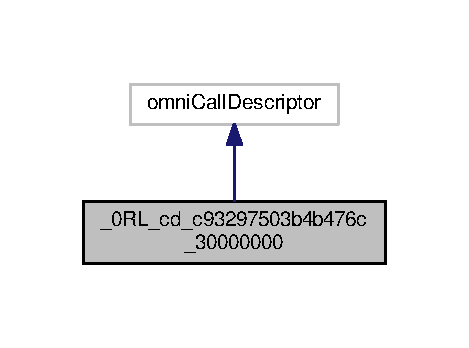
\includegraphics[width=225pt]{class__0_r_l__cd__c93297503b4b476c__30000000__inherit__graph}
\end{center}
\end{figure}


Collaboration diagram for \+\_\+0\+R\+L\+\_\+cd\+\_\+c93297503b4b476c\+\_\+30000000\+:
\nopagebreak
\begin{figure}[H]
\begin{center}
\leavevmode
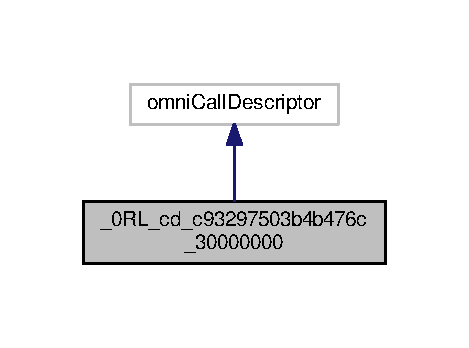
\includegraphics[width=225pt]{class__0_r_l__cd__c93297503b4b476c__30000000__coll__graph}
\end{center}
\end{figure}
\subsection*{Public Member Functions}
\begin{DoxyCompactItemize}
\item 
\hyperlink{class__0_r_l__cd__c93297503b4b476c__30000000_ae181c7b1d7848e49c70a52073b061400}{\+\_\+0\+R\+L\+\_\+cd\+\_\+c93297503b4b476c\+\_\+30000000} (Local\+Call\+Fn lcfn, const char $\ast$op\+\_\+, size\+\_\+t oplen, \+\_\+\+C\+O\+R\+B\+A\+\_\+\+Boolean upcall=0)
\item 
void \hyperlink{class__0_r_l__cd__c93297503b4b476c__30000000_a5acf7bd554776e260310ff9b60a28cc9}{marshal\+Arguments} (cdr\+Stream \&)
\item 
void \hyperlink{class__0_r_l__cd__c93297503b4b476c__30000000_a54388faf34b2345e350f1948e61fa147}{unmarshal\+Arguments} (cdr\+Stream \&)
\end{DoxyCompactItemize}
\subsection*{Public Attributes}
\begin{DoxyCompactItemize}
\item 
\+::C\+O\+R\+B\+A\+::\+Long \hyperlink{class__0_r_l__cd__c93297503b4b476c__30000000_a508ca8a434376dd8600660a60e41d84d}{arg\+\_\+0}
\item 
\+::C\+O\+R\+B\+A\+::\+Double \hyperlink{class__0_r_l__cd__c93297503b4b476c__30000000_a84a569f3464f78e8a47f0c154dd7e164}{arg\+\_\+1}
\end{DoxyCompactItemize}
\subsection*{Static Public Attributes}
\begin{DoxyCompactItemize}
\item 
static const char $\ast$const \hyperlink{class__0_r_l__cd__c93297503b4b476c__30000000_a49bdb6f8215069d7d5e9d5b93ab33cf5}{\+\_\+user\+\_\+exns} \mbox{[}$\,$\mbox{]}
\end{DoxyCompactItemize}


\subsection{Detailed Description}


Definition at line 1192 of file Petit\+Prince\+\_\+\+Stub.\+cpp.



\subsection{Constructor \& Destructor Documentation}
\index{\+\_\+0\+R\+L\+\_\+cd\+\_\+c93297503b4b476c\+\_\+30000000@{\+\_\+0\+R\+L\+\_\+cd\+\_\+c93297503b4b476c\+\_\+30000000}!\+\_\+0\+R\+L\+\_\+cd\+\_\+c93297503b4b476c\+\_\+30000000@{\+\_\+0\+R\+L\+\_\+cd\+\_\+c93297503b4b476c\+\_\+30000000}}
\index{\+\_\+0\+R\+L\+\_\+cd\+\_\+c93297503b4b476c\+\_\+30000000@{\+\_\+0\+R\+L\+\_\+cd\+\_\+c93297503b4b476c\+\_\+30000000}!\+\_\+0\+R\+L\+\_\+cd\+\_\+c93297503b4b476c\+\_\+30000000@{\+\_\+0\+R\+L\+\_\+cd\+\_\+c93297503b4b476c\+\_\+30000000}}
\subsubsection[{\texorpdfstring{\+\_\+0\+R\+L\+\_\+cd\+\_\+c93297503b4b476c\+\_\+30000000(\+Local\+Call\+Fn lcfn, const char $\ast$op\+\_\+, size\+\_\+t oplen, \+\_\+\+C\+O\+R\+B\+A\+\_\+\+Boolean upcall=0)}{_0RL_cd_c93297503b4b476c_30000000(LocalCallFn lcfn, const char *op_, size_t oplen, _CORBA_Boolean upcall=0)}}]{\setlength{\rightskip}{0pt plus 5cm}\+\_\+0\+R\+L\+\_\+cd\+\_\+c93297503b4b476c\+\_\+30000000\+::\+\_\+0\+R\+L\+\_\+cd\+\_\+c93297503b4b476c\+\_\+30000000 (
\begin{DoxyParamCaption}
\item[{Local\+Call\+Fn}]{lcfn, }
\item[{const char $\ast$}]{op\+\_\+, }
\item[{size\+\_\+t}]{oplen, }
\item[{\+\_\+\+C\+O\+R\+B\+A\+\_\+\+Boolean}]{upcall = {\ttfamily 0}}
\end{DoxyParamCaption}
)\hspace{0.3cm}{\ttfamily [inline]}}\hypertarget{class__0_r_l__cd__c93297503b4b476c__30000000_ae181c7b1d7848e49c70a52073b061400}{}\label{class__0_r_l__cd__c93297503b4b476c__30000000_ae181c7b1d7848e49c70a52073b061400}


Definition at line 1196 of file Petit\+Prince\+\_\+\+Stub.\+cpp.



\subsection{Member Function Documentation}
\index{\+\_\+0\+R\+L\+\_\+cd\+\_\+c93297503b4b476c\+\_\+30000000@{\+\_\+0\+R\+L\+\_\+cd\+\_\+c93297503b4b476c\+\_\+30000000}!marshal\+Arguments@{marshal\+Arguments}}
\index{marshal\+Arguments@{marshal\+Arguments}!\+\_\+0\+R\+L\+\_\+cd\+\_\+c93297503b4b476c\+\_\+30000000@{\+\_\+0\+R\+L\+\_\+cd\+\_\+c93297503b4b476c\+\_\+30000000}}
\subsubsection[{\texorpdfstring{marshal\+Arguments(cdr\+Stream \&)}{marshalArguments(cdrStream &)}}]{\setlength{\rightskip}{0pt plus 5cm}void \+\_\+0\+R\+L\+\_\+cd\+\_\+c93297503b4b476c\+\_\+30000000\+::marshal\+Arguments (
\begin{DoxyParamCaption}
\item[{cdr\+Stream \&}]{\+\_\+n}
\end{DoxyParamCaption}
)}\hypertarget{class__0_r_l__cd__c93297503b4b476c__30000000_a5acf7bd554776e260310ff9b60a28cc9}{}\label{class__0_r_l__cd__c93297503b4b476c__30000000_a5acf7bd554776e260310ff9b60a28cc9}


Definition at line 1213 of file Petit\+Prince\+\_\+\+Stub.\+cpp.

\index{\+\_\+0\+R\+L\+\_\+cd\+\_\+c93297503b4b476c\+\_\+30000000@{\+\_\+0\+R\+L\+\_\+cd\+\_\+c93297503b4b476c\+\_\+30000000}!unmarshal\+Arguments@{unmarshal\+Arguments}}
\index{unmarshal\+Arguments@{unmarshal\+Arguments}!\+\_\+0\+R\+L\+\_\+cd\+\_\+c93297503b4b476c\+\_\+30000000@{\+\_\+0\+R\+L\+\_\+cd\+\_\+c93297503b4b476c\+\_\+30000000}}
\subsubsection[{\texorpdfstring{unmarshal\+Arguments(cdr\+Stream \&)}{unmarshalArguments(cdrStream &)}}]{\setlength{\rightskip}{0pt plus 5cm}void \+\_\+0\+R\+L\+\_\+cd\+\_\+c93297503b4b476c\+\_\+30000000\+::unmarshal\+Arguments (
\begin{DoxyParamCaption}
\item[{cdr\+Stream \&}]{\+\_\+n}
\end{DoxyParamCaption}
)}\hypertarget{class__0_r_l__cd__c93297503b4b476c__30000000_a54388faf34b2345e350f1948e61fa147}{}\label{class__0_r_l__cd__c93297503b4b476c__30000000_a54388faf34b2345e350f1948e61fa147}


Definition at line 1220 of file Petit\+Prince\+\_\+\+Stub.\+cpp.



\subsection{Member Data Documentation}
\index{\+\_\+0\+R\+L\+\_\+cd\+\_\+c93297503b4b476c\+\_\+30000000@{\+\_\+0\+R\+L\+\_\+cd\+\_\+c93297503b4b476c\+\_\+30000000}!\+\_\+user\+\_\+exns@{\+\_\+user\+\_\+exns}}
\index{\+\_\+user\+\_\+exns@{\+\_\+user\+\_\+exns}!\+\_\+0\+R\+L\+\_\+cd\+\_\+c93297503b4b476c\+\_\+30000000@{\+\_\+0\+R\+L\+\_\+cd\+\_\+c93297503b4b476c\+\_\+30000000}}
\subsubsection[{\texorpdfstring{\+\_\+user\+\_\+exns}{_user_exns}}]{\setlength{\rightskip}{0pt plus 5cm}const char $\ast$const \+\_\+0\+R\+L\+\_\+cd\+\_\+c93297503b4b476c\+\_\+30000000\+::\+\_\+user\+\_\+exns\hspace{0.3cm}{\ttfamily [static]}}\hypertarget{class__0_r_l__cd__c93297503b4b476c__30000000_a49bdb6f8215069d7d5e9d5b93ab33cf5}{}\label{class__0_r_l__cd__c93297503b4b476c__30000000_a49bdb6f8215069d7d5e9d5b93ab33cf5}
{\bfseries Initial value\+:}
\begin{DoxyCode}
= \{
  0
\}
\end{DoxyCode}


Definition at line 1207 of file Petit\+Prince\+\_\+\+Stub.\+cpp.

\index{\+\_\+0\+R\+L\+\_\+cd\+\_\+c93297503b4b476c\+\_\+30000000@{\+\_\+0\+R\+L\+\_\+cd\+\_\+c93297503b4b476c\+\_\+30000000}!arg\+\_\+0@{arg\+\_\+0}}
\index{arg\+\_\+0@{arg\+\_\+0}!\+\_\+0\+R\+L\+\_\+cd\+\_\+c93297503b4b476c\+\_\+30000000@{\+\_\+0\+R\+L\+\_\+cd\+\_\+c93297503b4b476c\+\_\+30000000}}
\subsubsection[{\texorpdfstring{arg\+\_\+0}{arg_0}}]{\setlength{\rightskip}{0pt plus 5cm}\+::C\+O\+R\+B\+A\+::\+Long \+\_\+0\+R\+L\+\_\+cd\+\_\+c93297503b4b476c\+\_\+30000000\+::arg\+\_\+0}\hypertarget{class__0_r_l__cd__c93297503b4b476c__30000000_a508ca8a434376dd8600660a60e41d84d}{}\label{class__0_r_l__cd__c93297503b4b476c__30000000_a508ca8a434376dd8600660a60e41d84d}


Definition at line 1209 of file Petit\+Prince\+\_\+\+Stub.\+cpp.

\index{\+\_\+0\+R\+L\+\_\+cd\+\_\+c93297503b4b476c\+\_\+30000000@{\+\_\+0\+R\+L\+\_\+cd\+\_\+c93297503b4b476c\+\_\+30000000}!arg\+\_\+1@{arg\+\_\+1}}
\index{arg\+\_\+1@{arg\+\_\+1}!\+\_\+0\+R\+L\+\_\+cd\+\_\+c93297503b4b476c\+\_\+30000000@{\+\_\+0\+R\+L\+\_\+cd\+\_\+c93297503b4b476c\+\_\+30000000}}
\subsubsection[{\texorpdfstring{arg\+\_\+1}{arg_1}}]{\setlength{\rightskip}{0pt plus 5cm}\+::C\+O\+R\+B\+A\+::\+Double \+\_\+0\+R\+L\+\_\+cd\+\_\+c93297503b4b476c\+\_\+30000000\+::arg\+\_\+1}\hypertarget{class__0_r_l__cd__c93297503b4b476c__30000000_a84a569f3464f78e8a47f0c154dd7e164}{}\label{class__0_r_l__cd__c93297503b4b476c__30000000_a84a569f3464f78e8a47f0c154dd7e164}


Definition at line 1210 of file Petit\+Prince\+\_\+\+Stub.\+cpp.



The documentation for this class was generated from the following file\+:\begin{DoxyCompactItemize}
\item 
src/\hyperlink{_petit_prince___stub_8cpp}{Petit\+Prince\+\_\+\+Stub.\+cpp}\end{DoxyCompactItemize}

\hypertarget{class__0_r_l__cd__c93297503b4b476c__31000000}{}\section{\+\_\+0\+R\+L\+\_\+cd\+\_\+c93297503b4b476c\+\_\+31000000 Class Reference}
\label{class__0_r_l__cd__c93297503b4b476c__31000000}\index{\+\_\+0\+R\+L\+\_\+cd\+\_\+c93297503b4b476c\+\_\+31000000@{\+\_\+0\+R\+L\+\_\+cd\+\_\+c93297503b4b476c\+\_\+31000000}}


Inheritance diagram for \+\_\+0\+R\+L\+\_\+cd\+\_\+c93297503b4b476c\+\_\+31000000\+:
\nopagebreak
\begin{figure}[H]
\begin{center}
\leavevmode
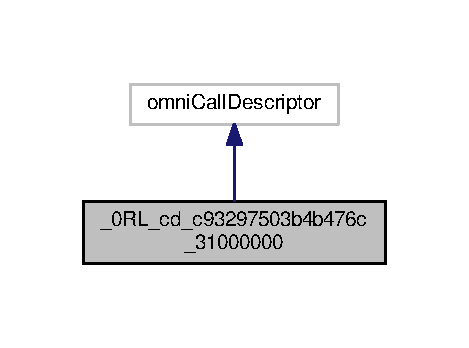
\includegraphics[width=225pt]{class__0_r_l__cd__c93297503b4b476c__31000000__inherit__graph}
\end{center}
\end{figure}


Collaboration diagram for \+\_\+0\+R\+L\+\_\+cd\+\_\+c93297503b4b476c\+\_\+31000000\+:
\nopagebreak
\begin{figure}[H]
\begin{center}
\leavevmode
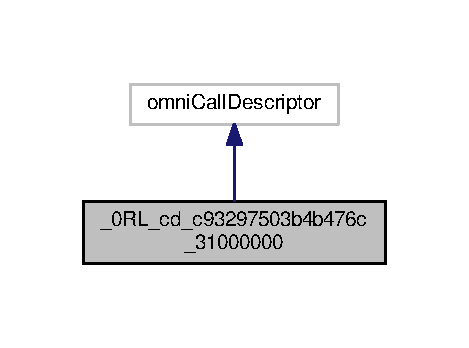
\includegraphics[width=225pt]{class__0_r_l__cd__c93297503b4b476c__31000000__coll__graph}
\end{center}
\end{figure}
\subsection*{Public Member Functions}
\begin{DoxyCompactItemize}
\item 
\hyperlink{class__0_r_l__cd__c93297503b4b476c__31000000_a47569d81948b4307436c980a6ef3c09e}{\+\_\+0\+R\+L\+\_\+cd\+\_\+c93297503b4b476c\+\_\+31000000} (Local\+Call\+Fn lcfn, const char $\ast$op\+\_\+, size\+\_\+t oplen, \+\_\+\+C\+O\+R\+B\+A\+\_\+\+Boolean upcall=0)
\item 
void \hyperlink{class__0_r_l__cd__c93297503b4b476c__31000000_a7e455e82866202c57a65e9a8d1a82b04}{marshal\+Arguments} (cdr\+Stream \&)
\item 
void \hyperlink{class__0_r_l__cd__c93297503b4b476c__31000000_ae8ad400b7c9b9380a51ae3a4eab854c3}{unmarshal\+Arguments} (cdr\+Stream \&)
\item 
void \hyperlink{class__0_r_l__cd__c93297503b4b476c__31000000_ad1c3afd1b1cabc40ae681a860e028842}{unmarshal\+Returned\+Values} (cdr\+Stream \&)
\item 
void \hyperlink{class__0_r_l__cd__c93297503b4b476c__31000000_a65934092e91506fde94dbe28eb952759}{marshal\+Returned\+Values} (cdr\+Stream \&)
\item 
void \hyperlink{class__0_r_l__cd__c93297503b4b476c__31000000_abf144e26cb2c3cbaa98e0ed2cdf5c66d}{user\+Exception} (cdr\+Stream \&, \+\_\+\+O\+M\+N\+I\+\_\+\+NS(I\+O\+P\+\_\+C)$\ast$, const char $\ast$)
\end{DoxyCompactItemize}
\subsection*{Public Attributes}
\begin{DoxyCompactItemize}
\item 
\+::C\+O\+R\+B\+A\+::\+String\+\_\+var \hyperlink{class__0_r_l__cd__c93297503b4b476c__31000000_a363b01496bb066cf3148298983a6f5ca}{arg\+\_\+0\+\_\+}
\item 
const char $\ast$ \hyperlink{class__0_r_l__cd__c93297503b4b476c__31000000_ab8f8fb171826c479fa1d20a6ae75bc8a}{arg\+\_\+0}
\item 
Petit\+Prince\+::\+Point \hyperlink{class__0_r_l__cd__c93297503b4b476c__31000000_abe834bb7ce68fa30fbf50962745bdd51}{arg\+\_\+1\+\_\+}
\item 
const Petit\+Prince\+::\+Point $\ast$ \hyperlink{class__0_r_l__cd__c93297503b4b476c__31000000_ad21353f2fa5950438e3ed7ca1077177b}{arg\+\_\+1}
\item 
\+::C\+O\+R\+B\+A\+::\+Double \hyperlink{class__0_r_l__cd__c93297503b4b476c__31000000_ad26a41851d02b94505f3e96984968453}{arg\+\_\+2}
\item 
\+::C\+O\+R\+B\+A\+::\+Double \hyperlink{class__0_r_l__cd__c93297503b4b476c__31000000_a836a674a6af5f0de805e77e06cf63fd5}{arg\+\_\+3}
\item 
\+::C\+O\+R\+B\+A\+::\+Long \hyperlink{class__0_r_l__cd__c93297503b4b476c__31000000_a6e7a1986f3ea1dda54668466a335a2e2}{result}
\end{DoxyCompactItemize}
\subsection*{Static Public Attributes}
\begin{DoxyCompactItemize}
\item 
static const char $\ast$const \hyperlink{class__0_r_l__cd__c93297503b4b476c__31000000_ab13e3318c54b3456b5e22c5264cea81e}{\+\_\+user\+\_\+exns} \mbox{[}$\,$\mbox{]}
\end{DoxyCompactItemize}


\subsection{Detailed Description}


Definition at line 2135 of file Petit\+Prince\+\_\+\+Stub.\+cpp.



\subsection{Constructor \& Destructor Documentation}
\index{\+\_\+0\+R\+L\+\_\+cd\+\_\+c93297503b4b476c\+\_\+31000000@{\+\_\+0\+R\+L\+\_\+cd\+\_\+c93297503b4b476c\+\_\+31000000}!\+\_\+0\+R\+L\+\_\+cd\+\_\+c93297503b4b476c\+\_\+31000000@{\+\_\+0\+R\+L\+\_\+cd\+\_\+c93297503b4b476c\+\_\+31000000}}
\index{\+\_\+0\+R\+L\+\_\+cd\+\_\+c93297503b4b476c\+\_\+31000000@{\+\_\+0\+R\+L\+\_\+cd\+\_\+c93297503b4b476c\+\_\+31000000}!\+\_\+0\+R\+L\+\_\+cd\+\_\+c93297503b4b476c\+\_\+31000000@{\+\_\+0\+R\+L\+\_\+cd\+\_\+c93297503b4b476c\+\_\+31000000}}
\subsubsection[{\texorpdfstring{\+\_\+0\+R\+L\+\_\+cd\+\_\+c93297503b4b476c\+\_\+31000000(\+Local\+Call\+Fn lcfn, const char $\ast$op\+\_\+, size\+\_\+t oplen, \+\_\+\+C\+O\+R\+B\+A\+\_\+\+Boolean upcall=0)}{_0RL_cd_c93297503b4b476c_31000000(LocalCallFn lcfn, const char *op_, size_t oplen, _CORBA_Boolean upcall=0)}}]{\setlength{\rightskip}{0pt plus 5cm}\+\_\+0\+R\+L\+\_\+cd\+\_\+c93297503b4b476c\+\_\+31000000\+::\+\_\+0\+R\+L\+\_\+cd\+\_\+c93297503b4b476c\+\_\+31000000 (
\begin{DoxyParamCaption}
\item[{Local\+Call\+Fn}]{lcfn, }
\item[{const char $\ast$}]{op\+\_\+, }
\item[{size\+\_\+t}]{oplen, }
\item[{\+\_\+\+C\+O\+R\+B\+A\+\_\+\+Boolean}]{upcall = {\ttfamily 0}}
\end{DoxyParamCaption}
)\hspace{0.3cm}{\ttfamily [inline]}}\hypertarget{class__0_r_l__cd__c93297503b4b476c__31000000_a47569d81948b4307436c980a6ef3c09e}{}\label{class__0_r_l__cd__c93297503b4b476c__31000000_a47569d81948b4307436c980a6ef3c09e}


Definition at line 2139 of file Petit\+Prince\+\_\+\+Stub.\+cpp.



\subsection{Member Function Documentation}
\index{\+\_\+0\+R\+L\+\_\+cd\+\_\+c93297503b4b476c\+\_\+31000000@{\+\_\+0\+R\+L\+\_\+cd\+\_\+c93297503b4b476c\+\_\+31000000}!marshal\+Arguments@{marshal\+Arguments}}
\index{marshal\+Arguments@{marshal\+Arguments}!\+\_\+0\+R\+L\+\_\+cd\+\_\+c93297503b4b476c\+\_\+31000000@{\+\_\+0\+R\+L\+\_\+cd\+\_\+c93297503b4b476c\+\_\+31000000}}
\subsubsection[{\texorpdfstring{marshal\+Arguments(cdr\+Stream \&)}{marshalArguments(cdrStream &)}}]{\setlength{\rightskip}{0pt plus 5cm}void \+\_\+0\+R\+L\+\_\+cd\+\_\+c93297503b4b476c\+\_\+31000000\+::marshal\+Arguments (
\begin{DoxyParamCaption}
\item[{cdr\+Stream \&}]{\+\_\+n}
\end{DoxyParamCaption}
)}\hypertarget{class__0_r_l__cd__c93297503b4b476c__31000000_a7e455e82866202c57a65e9a8d1a82b04}{}\label{class__0_r_l__cd__c93297503b4b476c__31000000_a7e455e82866202c57a65e9a8d1a82b04}


Definition at line 2163 of file Petit\+Prince\+\_\+\+Stub.\+cpp.

\index{\+\_\+0\+R\+L\+\_\+cd\+\_\+c93297503b4b476c\+\_\+31000000@{\+\_\+0\+R\+L\+\_\+cd\+\_\+c93297503b4b476c\+\_\+31000000}!marshal\+Returned\+Values@{marshal\+Returned\+Values}}
\index{marshal\+Returned\+Values@{marshal\+Returned\+Values}!\+\_\+0\+R\+L\+\_\+cd\+\_\+c93297503b4b476c\+\_\+31000000@{\+\_\+0\+R\+L\+\_\+cd\+\_\+c93297503b4b476c\+\_\+31000000}}
\subsubsection[{\texorpdfstring{marshal\+Returned\+Values(cdr\+Stream \&)}{marshalReturnedValues(cdrStream &)}}]{\setlength{\rightskip}{0pt plus 5cm}void \+\_\+0\+R\+L\+\_\+cd\+\_\+c93297503b4b476c\+\_\+31000000\+::marshal\+Returned\+Values (
\begin{DoxyParamCaption}
\item[{cdr\+Stream \&}]{\+\_\+n}
\end{DoxyParamCaption}
)}\hypertarget{class__0_r_l__cd__c93297503b4b476c__31000000_a65934092e91506fde94dbe28eb952759}{}\label{class__0_r_l__cd__c93297503b4b476c__31000000_a65934092e91506fde94dbe28eb952759}


Definition at line 2183 of file Petit\+Prince\+\_\+\+Stub.\+cpp.

\index{\+\_\+0\+R\+L\+\_\+cd\+\_\+c93297503b4b476c\+\_\+31000000@{\+\_\+0\+R\+L\+\_\+cd\+\_\+c93297503b4b476c\+\_\+31000000}!unmarshal\+Arguments@{unmarshal\+Arguments}}
\index{unmarshal\+Arguments@{unmarshal\+Arguments}!\+\_\+0\+R\+L\+\_\+cd\+\_\+c93297503b4b476c\+\_\+31000000@{\+\_\+0\+R\+L\+\_\+cd\+\_\+c93297503b4b476c\+\_\+31000000}}
\subsubsection[{\texorpdfstring{unmarshal\+Arguments(cdr\+Stream \&)}{unmarshalArguments(cdrStream &)}}]{\setlength{\rightskip}{0pt plus 5cm}void \+\_\+0\+R\+L\+\_\+cd\+\_\+c93297503b4b476c\+\_\+31000000\+::unmarshal\+Arguments (
\begin{DoxyParamCaption}
\item[{cdr\+Stream \&}]{\+\_\+n}
\end{DoxyParamCaption}
)}\hypertarget{class__0_r_l__cd__c93297503b4b476c__31000000_ae8ad400b7c9b9380a51ae3a4eab854c3}{}\label{class__0_r_l__cd__c93297503b4b476c__31000000_ae8ad400b7c9b9380a51ae3a4eab854c3}


Definition at line 2172 of file Petit\+Prince\+\_\+\+Stub.\+cpp.

\index{\+\_\+0\+R\+L\+\_\+cd\+\_\+c93297503b4b476c\+\_\+31000000@{\+\_\+0\+R\+L\+\_\+cd\+\_\+c93297503b4b476c\+\_\+31000000}!unmarshal\+Returned\+Values@{unmarshal\+Returned\+Values}}
\index{unmarshal\+Returned\+Values@{unmarshal\+Returned\+Values}!\+\_\+0\+R\+L\+\_\+cd\+\_\+c93297503b4b476c\+\_\+31000000@{\+\_\+0\+R\+L\+\_\+cd\+\_\+c93297503b4b476c\+\_\+31000000}}
\subsubsection[{\texorpdfstring{unmarshal\+Returned\+Values(cdr\+Stream \&)}{unmarshalReturnedValues(cdrStream &)}}]{\setlength{\rightskip}{0pt plus 5cm}void \+\_\+0\+R\+L\+\_\+cd\+\_\+c93297503b4b476c\+\_\+31000000\+::unmarshal\+Returned\+Values (
\begin{DoxyParamCaption}
\item[{cdr\+Stream \&}]{\+\_\+n}
\end{DoxyParamCaption}
)}\hypertarget{class__0_r_l__cd__c93297503b4b476c__31000000_ad1c3afd1b1cabc40ae681a860e028842}{}\label{class__0_r_l__cd__c93297503b4b476c__31000000_ad1c3afd1b1cabc40ae681a860e028842}


Definition at line 2189 of file Petit\+Prince\+\_\+\+Stub.\+cpp.

\index{\+\_\+0\+R\+L\+\_\+cd\+\_\+c93297503b4b476c\+\_\+31000000@{\+\_\+0\+R\+L\+\_\+cd\+\_\+c93297503b4b476c\+\_\+31000000}!user\+Exception@{user\+Exception}}
\index{user\+Exception@{user\+Exception}!\+\_\+0\+R\+L\+\_\+cd\+\_\+c93297503b4b476c\+\_\+31000000@{\+\_\+0\+R\+L\+\_\+cd\+\_\+c93297503b4b476c\+\_\+31000000}}
\subsubsection[{\texorpdfstring{user\+Exception(cdr\+Stream \&, \+\_\+\+O\+M\+N\+I\+\_\+\+N\+S(\+I\+O\+P\+\_\+\+C)$\ast$, const char $\ast$)}{userException(cdrStream &, _OMNI_NS(IOP_C)*, const char *)}}]{\setlength{\rightskip}{0pt plus 5cm}void \+\_\+0\+R\+L\+\_\+cd\+\_\+c93297503b4b476c\+\_\+31000000\+::user\+Exception (
\begin{DoxyParamCaption}
\item[{cdr\+Stream \&}]{s, }
\item[{\+\_\+\+O\+M\+N\+I\+\_\+\+NS(I\+O\+P\+\_\+C)$\ast$}]{iop\+\_\+client, }
\item[{const char $\ast$}]{repo\+Id}
\end{DoxyParamCaption}
)}\hypertarget{class__0_r_l__cd__c93297503b4b476c__31000000_abf144e26cb2c3cbaa98e0ed2cdf5c66d}{}\label{class__0_r_l__cd__c93297503b4b476c__31000000_abf144e26cb2c3cbaa98e0ed2cdf5c66d}


Definition at line 2199 of file Petit\+Prince\+\_\+\+Stub.\+cpp.



\subsection{Member Data Documentation}
\index{\+\_\+0\+R\+L\+\_\+cd\+\_\+c93297503b4b476c\+\_\+31000000@{\+\_\+0\+R\+L\+\_\+cd\+\_\+c93297503b4b476c\+\_\+31000000}!\+\_\+user\+\_\+exns@{\+\_\+user\+\_\+exns}}
\index{\+\_\+user\+\_\+exns@{\+\_\+user\+\_\+exns}!\+\_\+0\+R\+L\+\_\+cd\+\_\+c93297503b4b476c\+\_\+31000000@{\+\_\+0\+R\+L\+\_\+cd\+\_\+c93297503b4b476c\+\_\+31000000}}
\subsubsection[{\texorpdfstring{\+\_\+user\+\_\+exns}{_user_exns}}]{\setlength{\rightskip}{0pt plus 5cm}const char $\ast$const \+\_\+0\+R\+L\+\_\+cd\+\_\+c93297503b4b476c\+\_\+31000000\+::\+\_\+user\+\_\+exns\hspace{0.3cm}{\ttfamily [static]}}\hypertarget{class__0_r_l__cd__c93297503b4b476c__31000000_ab13e3318c54b3456b5e22c5264cea81e}{}\label{class__0_r_l__cd__c93297503b4b476c__31000000_ab13e3318c54b3456b5e22c5264cea81e}
{\bfseries Initial value\+:}
\begin{DoxyCode}
= \{
  PetitPrince::PetitPrinceService::InvalidDrawParams::\_PD\_repoId
\}
\end{DoxyCode}


Definition at line 2152 of file Petit\+Prince\+\_\+\+Stub.\+cpp.

\index{\+\_\+0\+R\+L\+\_\+cd\+\_\+c93297503b4b476c\+\_\+31000000@{\+\_\+0\+R\+L\+\_\+cd\+\_\+c93297503b4b476c\+\_\+31000000}!arg\+\_\+0@{arg\+\_\+0}}
\index{arg\+\_\+0@{arg\+\_\+0}!\+\_\+0\+R\+L\+\_\+cd\+\_\+c93297503b4b476c\+\_\+31000000@{\+\_\+0\+R\+L\+\_\+cd\+\_\+c93297503b4b476c\+\_\+31000000}}
\subsubsection[{\texorpdfstring{arg\+\_\+0}{arg_0}}]{\setlength{\rightskip}{0pt plus 5cm}const char$\ast$ \+\_\+0\+R\+L\+\_\+cd\+\_\+c93297503b4b476c\+\_\+31000000\+::arg\+\_\+0}\hypertarget{class__0_r_l__cd__c93297503b4b476c__31000000_ab8f8fb171826c479fa1d20a6ae75bc8a}{}\label{class__0_r_l__cd__c93297503b4b476c__31000000_ab8f8fb171826c479fa1d20a6ae75bc8a}


Definition at line 2155 of file Petit\+Prince\+\_\+\+Stub.\+cpp.

\index{\+\_\+0\+R\+L\+\_\+cd\+\_\+c93297503b4b476c\+\_\+31000000@{\+\_\+0\+R\+L\+\_\+cd\+\_\+c93297503b4b476c\+\_\+31000000}!arg\+\_\+0\+\_\+@{arg\+\_\+0\+\_\+}}
\index{arg\+\_\+0\+\_\+@{arg\+\_\+0\+\_\+}!\+\_\+0\+R\+L\+\_\+cd\+\_\+c93297503b4b476c\+\_\+31000000@{\+\_\+0\+R\+L\+\_\+cd\+\_\+c93297503b4b476c\+\_\+31000000}}
\subsubsection[{\texorpdfstring{arg\+\_\+0\+\_\+}{arg_0_}}]{\setlength{\rightskip}{0pt plus 5cm}\+::C\+O\+R\+B\+A\+::\+String\+\_\+var \+\_\+0\+R\+L\+\_\+cd\+\_\+c93297503b4b476c\+\_\+31000000\+::arg\+\_\+0\+\_\+}\hypertarget{class__0_r_l__cd__c93297503b4b476c__31000000_a363b01496bb066cf3148298983a6f5ca}{}\label{class__0_r_l__cd__c93297503b4b476c__31000000_a363b01496bb066cf3148298983a6f5ca}


Definition at line 2154 of file Petit\+Prince\+\_\+\+Stub.\+cpp.

\index{\+\_\+0\+R\+L\+\_\+cd\+\_\+c93297503b4b476c\+\_\+31000000@{\+\_\+0\+R\+L\+\_\+cd\+\_\+c93297503b4b476c\+\_\+31000000}!arg\+\_\+1@{arg\+\_\+1}}
\index{arg\+\_\+1@{arg\+\_\+1}!\+\_\+0\+R\+L\+\_\+cd\+\_\+c93297503b4b476c\+\_\+31000000@{\+\_\+0\+R\+L\+\_\+cd\+\_\+c93297503b4b476c\+\_\+31000000}}
\subsubsection[{\texorpdfstring{arg\+\_\+1}{arg_1}}]{\setlength{\rightskip}{0pt plus 5cm}const Petit\+Prince\+::\+Point$\ast$ \+\_\+0\+R\+L\+\_\+cd\+\_\+c93297503b4b476c\+\_\+31000000\+::arg\+\_\+1}\hypertarget{class__0_r_l__cd__c93297503b4b476c__31000000_ad21353f2fa5950438e3ed7ca1077177b}{}\label{class__0_r_l__cd__c93297503b4b476c__31000000_ad21353f2fa5950438e3ed7ca1077177b}


Definition at line 2157 of file Petit\+Prince\+\_\+\+Stub.\+cpp.

\index{\+\_\+0\+R\+L\+\_\+cd\+\_\+c93297503b4b476c\+\_\+31000000@{\+\_\+0\+R\+L\+\_\+cd\+\_\+c93297503b4b476c\+\_\+31000000}!arg\+\_\+1\+\_\+@{arg\+\_\+1\+\_\+}}
\index{arg\+\_\+1\+\_\+@{arg\+\_\+1\+\_\+}!\+\_\+0\+R\+L\+\_\+cd\+\_\+c93297503b4b476c\+\_\+31000000@{\+\_\+0\+R\+L\+\_\+cd\+\_\+c93297503b4b476c\+\_\+31000000}}
\subsubsection[{\texorpdfstring{arg\+\_\+1\+\_\+}{arg_1_}}]{\setlength{\rightskip}{0pt plus 5cm}Petit\+Prince\+::\+Point \+\_\+0\+R\+L\+\_\+cd\+\_\+c93297503b4b476c\+\_\+31000000\+::arg\+\_\+1\+\_\+}\hypertarget{class__0_r_l__cd__c93297503b4b476c__31000000_abe834bb7ce68fa30fbf50962745bdd51}{}\label{class__0_r_l__cd__c93297503b4b476c__31000000_abe834bb7ce68fa30fbf50962745bdd51}


Definition at line 2156 of file Petit\+Prince\+\_\+\+Stub.\+cpp.

\index{\+\_\+0\+R\+L\+\_\+cd\+\_\+c93297503b4b476c\+\_\+31000000@{\+\_\+0\+R\+L\+\_\+cd\+\_\+c93297503b4b476c\+\_\+31000000}!arg\+\_\+2@{arg\+\_\+2}}
\index{arg\+\_\+2@{arg\+\_\+2}!\+\_\+0\+R\+L\+\_\+cd\+\_\+c93297503b4b476c\+\_\+31000000@{\+\_\+0\+R\+L\+\_\+cd\+\_\+c93297503b4b476c\+\_\+31000000}}
\subsubsection[{\texorpdfstring{arg\+\_\+2}{arg_2}}]{\setlength{\rightskip}{0pt plus 5cm}\+::C\+O\+R\+B\+A\+::\+Double \+\_\+0\+R\+L\+\_\+cd\+\_\+c93297503b4b476c\+\_\+31000000\+::arg\+\_\+2}\hypertarget{class__0_r_l__cd__c93297503b4b476c__31000000_ad26a41851d02b94505f3e96984968453}{}\label{class__0_r_l__cd__c93297503b4b476c__31000000_ad26a41851d02b94505f3e96984968453}


Definition at line 2158 of file Petit\+Prince\+\_\+\+Stub.\+cpp.

\index{\+\_\+0\+R\+L\+\_\+cd\+\_\+c93297503b4b476c\+\_\+31000000@{\+\_\+0\+R\+L\+\_\+cd\+\_\+c93297503b4b476c\+\_\+31000000}!arg\+\_\+3@{arg\+\_\+3}}
\index{arg\+\_\+3@{arg\+\_\+3}!\+\_\+0\+R\+L\+\_\+cd\+\_\+c93297503b4b476c\+\_\+31000000@{\+\_\+0\+R\+L\+\_\+cd\+\_\+c93297503b4b476c\+\_\+31000000}}
\subsubsection[{\texorpdfstring{arg\+\_\+3}{arg_3}}]{\setlength{\rightskip}{0pt plus 5cm}\+::C\+O\+R\+B\+A\+::\+Double \+\_\+0\+R\+L\+\_\+cd\+\_\+c93297503b4b476c\+\_\+31000000\+::arg\+\_\+3}\hypertarget{class__0_r_l__cd__c93297503b4b476c__31000000_a836a674a6af5f0de805e77e06cf63fd5}{}\label{class__0_r_l__cd__c93297503b4b476c__31000000_a836a674a6af5f0de805e77e06cf63fd5}


Definition at line 2159 of file Petit\+Prince\+\_\+\+Stub.\+cpp.

\index{\+\_\+0\+R\+L\+\_\+cd\+\_\+c93297503b4b476c\+\_\+31000000@{\+\_\+0\+R\+L\+\_\+cd\+\_\+c93297503b4b476c\+\_\+31000000}!result@{result}}
\index{result@{result}!\+\_\+0\+R\+L\+\_\+cd\+\_\+c93297503b4b476c\+\_\+31000000@{\+\_\+0\+R\+L\+\_\+cd\+\_\+c93297503b4b476c\+\_\+31000000}}
\subsubsection[{\texorpdfstring{result}{result}}]{\setlength{\rightskip}{0pt plus 5cm}\+::C\+O\+R\+B\+A\+::\+Long \+\_\+0\+R\+L\+\_\+cd\+\_\+c93297503b4b476c\+\_\+31000000\+::result}\hypertarget{class__0_r_l__cd__c93297503b4b476c__31000000_a6e7a1986f3ea1dda54668466a335a2e2}{}\label{class__0_r_l__cd__c93297503b4b476c__31000000_a6e7a1986f3ea1dda54668466a335a2e2}


Definition at line 2160 of file Petit\+Prince\+\_\+\+Stub.\+cpp.



The documentation for this class was generated from the following file\+:\begin{DoxyCompactItemize}
\item 
src/\hyperlink{_petit_prince___stub_8cpp}{Petit\+Prince\+\_\+\+Stub.\+cpp}\end{DoxyCompactItemize}

\hypertarget{class__0_r_l__cd__c93297503b4b476c__50000000}{}\section{\+\_\+0\+R\+L\+\_\+cd\+\_\+c93297503b4b476c\+\_\+50000000 Class Reference}
\label{class__0_r_l__cd__c93297503b4b476c__50000000}\index{\+\_\+0\+R\+L\+\_\+cd\+\_\+c93297503b4b476c\+\_\+50000000@{\+\_\+0\+R\+L\+\_\+cd\+\_\+c93297503b4b476c\+\_\+50000000}}


Inheritance diagram for \+\_\+0\+R\+L\+\_\+cd\+\_\+c93297503b4b476c\+\_\+50000000\+:
\nopagebreak
\begin{figure}[H]
\begin{center}
\leavevmode
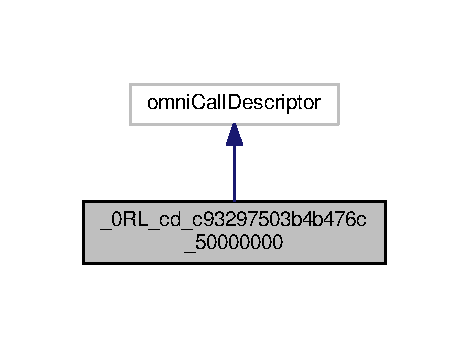
\includegraphics[width=225pt]{class__0_r_l__cd__c93297503b4b476c__50000000__inherit__graph}
\end{center}
\end{figure}


Collaboration diagram for \+\_\+0\+R\+L\+\_\+cd\+\_\+c93297503b4b476c\+\_\+50000000\+:
\nopagebreak
\begin{figure}[H]
\begin{center}
\leavevmode
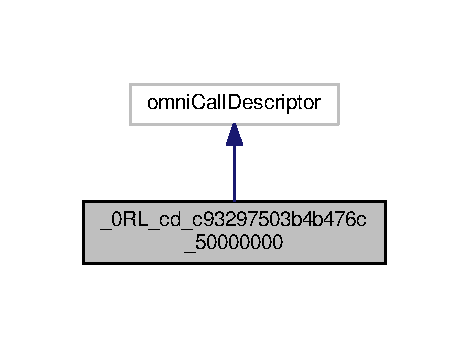
\includegraphics[width=225pt]{class__0_r_l__cd__c93297503b4b476c__50000000__coll__graph}
\end{center}
\end{figure}
\subsection*{Public Member Functions}
\begin{DoxyCompactItemize}
\item 
\hyperlink{class__0_r_l__cd__c93297503b4b476c__50000000_a0969c7fefe88982e32a15b255cbd6444}{\+\_\+0\+R\+L\+\_\+cd\+\_\+c93297503b4b476c\+\_\+50000000} (Local\+Call\+Fn lcfn, const char $\ast$op\+\_\+, size\+\_\+t oplen, \+\_\+\+C\+O\+R\+B\+A\+\_\+\+Boolean upcall=0)
\item 
void \hyperlink{class__0_r_l__cd__c93297503b4b476c__50000000_a555f809315838ca64716c409ff1cc821}{marshal\+Arguments} (cdr\+Stream \&)
\item 
void \hyperlink{class__0_r_l__cd__c93297503b4b476c__50000000_a81eb249414388136f92fd9f584475a77}{unmarshal\+Arguments} (cdr\+Stream \&)
\end{DoxyCompactItemize}
\subsection*{Public Attributes}
\begin{DoxyCompactItemize}
\item 
\+::C\+O\+R\+B\+A\+::\+Long \hyperlink{class__0_r_l__cd__c93297503b4b476c__50000000_adf874b79561a94362612a9a66efe8367}{arg\+\_\+0}
\item 
\+::C\+O\+R\+B\+A\+::\+Double \hyperlink{class__0_r_l__cd__c93297503b4b476c__50000000_a47d6cd5ebcdbf217e29a25baba671df8}{arg\+\_\+1}
\item 
\+::C\+O\+R\+B\+A\+::\+Double \hyperlink{class__0_r_l__cd__c93297503b4b476c__50000000_a6db84fccb3f773ae9dcf309b0b7e3682}{arg\+\_\+2}
\end{DoxyCompactItemize}
\subsection*{Static Public Attributes}
\begin{DoxyCompactItemize}
\item 
static const char $\ast$const \hyperlink{class__0_r_l__cd__c93297503b4b476c__50000000_ab515d885d1083c80fcaf70a6878e41e6}{\+\_\+user\+\_\+exns} \mbox{[}$\,$\mbox{]}
\end{DoxyCompactItemize}


\subsection{Constructor \& Destructor Documentation}
\index{\+\_\+0\+R\+L\+\_\+cd\+\_\+c93297503b4b476c\+\_\+50000000@{\+\_\+0\+R\+L\+\_\+cd\+\_\+c93297503b4b476c\+\_\+50000000}!\+\_\+0\+R\+L\+\_\+cd\+\_\+c93297503b4b476c\+\_\+50000000@{\+\_\+0\+R\+L\+\_\+cd\+\_\+c93297503b4b476c\+\_\+50000000}}
\index{\+\_\+0\+R\+L\+\_\+cd\+\_\+c93297503b4b476c\+\_\+50000000@{\+\_\+0\+R\+L\+\_\+cd\+\_\+c93297503b4b476c\+\_\+50000000}!\+\_\+0\+R\+L\+\_\+cd\+\_\+c93297503b4b476c\+\_\+50000000@{\+\_\+0\+R\+L\+\_\+cd\+\_\+c93297503b4b476c\+\_\+50000000}}
\subsubsection[{\texorpdfstring{\+\_\+0\+R\+L\+\_\+cd\+\_\+c93297503b4b476c\+\_\+50000000(\+Local\+Call\+Fn lcfn, const char $\ast$op\+\_\+, size\+\_\+t oplen, \+\_\+\+C\+O\+R\+B\+A\+\_\+\+Boolean upcall=0)}{_0RL_cd_c93297503b4b476c_50000000(LocalCallFn lcfn, const char *op_, size_t oplen, _CORBA_Boolean upcall=0)}}]{\setlength{\rightskip}{0pt plus 5cm}\+\_\+0\+R\+L\+\_\+cd\+\_\+c93297503b4b476c\+\_\+50000000\+::\+\_\+0\+R\+L\+\_\+cd\+\_\+c93297503b4b476c\+\_\+50000000 (
\begin{DoxyParamCaption}
\item[{Local\+Call\+Fn}]{lcfn, }
\item[{const char $\ast$}]{op\+\_\+, }
\item[{size\+\_\+t}]{oplen, }
\item[{\+\_\+\+C\+O\+R\+B\+A\+\_\+\+Boolean}]{upcall = {\ttfamily 0}}
\end{DoxyParamCaption}
)\hspace{0.3cm}{\ttfamily [inline]}}\hypertarget{class__0_r_l__cd__c93297503b4b476c__50000000_a0969c7fefe88982e32a15b255cbd6444}{}\label{class__0_r_l__cd__c93297503b4b476c__50000000_a0969c7fefe88982e32a15b255cbd6444}


\subsection{Member Function Documentation}
\index{\+\_\+0\+R\+L\+\_\+cd\+\_\+c93297503b4b476c\+\_\+50000000@{\+\_\+0\+R\+L\+\_\+cd\+\_\+c93297503b4b476c\+\_\+50000000}!marshal\+Arguments@{marshal\+Arguments}}
\index{marshal\+Arguments@{marshal\+Arguments}!\+\_\+0\+R\+L\+\_\+cd\+\_\+c93297503b4b476c\+\_\+50000000@{\+\_\+0\+R\+L\+\_\+cd\+\_\+c93297503b4b476c\+\_\+50000000}}
\subsubsection[{\texorpdfstring{marshal\+Arguments(cdr\+Stream \&)}{marshalArguments(cdrStream &)}}]{\setlength{\rightskip}{0pt plus 5cm}void \+\_\+0\+R\+L\+\_\+cd\+\_\+c93297503b4b476c\+\_\+50000000\+::marshal\+Arguments (
\begin{DoxyParamCaption}
\item[{cdr\+Stream \&}]{\+\_\+n}
\end{DoxyParamCaption}
)}\hypertarget{class__0_r_l__cd__c93297503b4b476c__50000000_a555f809315838ca64716c409ff1cc821}{}\label{class__0_r_l__cd__c93297503b4b476c__50000000_a555f809315838ca64716c409ff1cc821}
\index{\+\_\+0\+R\+L\+\_\+cd\+\_\+c93297503b4b476c\+\_\+50000000@{\+\_\+0\+R\+L\+\_\+cd\+\_\+c93297503b4b476c\+\_\+50000000}!unmarshal\+Arguments@{unmarshal\+Arguments}}
\index{unmarshal\+Arguments@{unmarshal\+Arguments}!\+\_\+0\+R\+L\+\_\+cd\+\_\+c93297503b4b476c\+\_\+50000000@{\+\_\+0\+R\+L\+\_\+cd\+\_\+c93297503b4b476c\+\_\+50000000}}
\subsubsection[{\texorpdfstring{unmarshal\+Arguments(cdr\+Stream \&)}{unmarshalArguments(cdrStream &)}}]{\setlength{\rightskip}{0pt plus 5cm}void \+\_\+0\+R\+L\+\_\+cd\+\_\+c93297503b4b476c\+\_\+50000000\+::unmarshal\+Arguments (
\begin{DoxyParamCaption}
\item[{cdr\+Stream \&}]{\+\_\+n}
\end{DoxyParamCaption}
)}\hypertarget{class__0_r_l__cd__c93297503b4b476c__50000000_a81eb249414388136f92fd9f584475a77}{}\label{class__0_r_l__cd__c93297503b4b476c__50000000_a81eb249414388136f92fd9f584475a77}


\subsection{Member Data Documentation}
\index{\+\_\+0\+R\+L\+\_\+cd\+\_\+c93297503b4b476c\+\_\+50000000@{\+\_\+0\+R\+L\+\_\+cd\+\_\+c93297503b4b476c\+\_\+50000000}!\+\_\+user\+\_\+exns@{\+\_\+user\+\_\+exns}}
\index{\+\_\+user\+\_\+exns@{\+\_\+user\+\_\+exns}!\+\_\+0\+R\+L\+\_\+cd\+\_\+c93297503b4b476c\+\_\+50000000@{\+\_\+0\+R\+L\+\_\+cd\+\_\+c93297503b4b476c\+\_\+50000000}}
\subsubsection[{\texorpdfstring{\+\_\+user\+\_\+exns}{_user_exns}}]{\setlength{\rightskip}{0pt plus 5cm}const char $\ast$const \+\_\+0\+R\+L\+\_\+cd\+\_\+c93297503b4b476c\+\_\+50000000\+::\+\_\+user\+\_\+exns\hspace{0.3cm}{\ttfamily [static]}}\hypertarget{class__0_r_l__cd__c93297503b4b476c__50000000_ab515d885d1083c80fcaf70a6878e41e6}{}\label{class__0_r_l__cd__c93297503b4b476c__50000000_ab515d885d1083c80fcaf70a6878e41e6}
{\bfseries Initial value\+:}
\begin{DoxyCode}
= \{
  0
\}
\end{DoxyCode}
\index{\+\_\+0\+R\+L\+\_\+cd\+\_\+c93297503b4b476c\+\_\+50000000@{\+\_\+0\+R\+L\+\_\+cd\+\_\+c93297503b4b476c\+\_\+50000000}!arg\+\_\+0@{arg\+\_\+0}}
\index{arg\+\_\+0@{arg\+\_\+0}!\+\_\+0\+R\+L\+\_\+cd\+\_\+c93297503b4b476c\+\_\+50000000@{\+\_\+0\+R\+L\+\_\+cd\+\_\+c93297503b4b476c\+\_\+50000000}}
\subsubsection[{\texorpdfstring{arg\+\_\+0}{arg_0}}]{\setlength{\rightskip}{0pt plus 5cm}\+::C\+O\+R\+B\+A\+::\+Long \+\_\+0\+R\+L\+\_\+cd\+\_\+c93297503b4b476c\+\_\+50000000\+::arg\+\_\+0}\hypertarget{class__0_r_l__cd__c93297503b4b476c__50000000_adf874b79561a94362612a9a66efe8367}{}\label{class__0_r_l__cd__c93297503b4b476c__50000000_adf874b79561a94362612a9a66efe8367}
\index{\+\_\+0\+R\+L\+\_\+cd\+\_\+c93297503b4b476c\+\_\+50000000@{\+\_\+0\+R\+L\+\_\+cd\+\_\+c93297503b4b476c\+\_\+50000000}!arg\+\_\+1@{arg\+\_\+1}}
\index{arg\+\_\+1@{arg\+\_\+1}!\+\_\+0\+R\+L\+\_\+cd\+\_\+c93297503b4b476c\+\_\+50000000@{\+\_\+0\+R\+L\+\_\+cd\+\_\+c93297503b4b476c\+\_\+50000000}}
\subsubsection[{\texorpdfstring{arg\+\_\+1}{arg_1}}]{\setlength{\rightskip}{0pt plus 5cm}\+::C\+O\+R\+B\+A\+::\+Double \+\_\+0\+R\+L\+\_\+cd\+\_\+c93297503b4b476c\+\_\+50000000\+::arg\+\_\+1}\hypertarget{class__0_r_l__cd__c93297503b4b476c__50000000_a47d6cd5ebcdbf217e29a25baba671df8}{}\label{class__0_r_l__cd__c93297503b4b476c__50000000_a47d6cd5ebcdbf217e29a25baba671df8}
\index{\+\_\+0\+R\+L\+\_\+cd\+\_\+c93297503b4b476c\+\_\+50000000@{\+\_\+0\+R\+L\+\_\+cd\+\_\+c93297503b4b476c\+\_\+50000000}!arg\+\_\+2@{arg\+\_\+2}}
\index{arg\+\_\+2@{arg\+\_\+2}!\+\_\+0\+R\+L\+\_\+cd\+\_\+c93297503b4b476c\+\_\+50000000@{\+\_\+0\+R\+L\+\_\+cd\+\_\+c93297503b4b476c\+\_\+50000000}}
\subsubsection[{\texorpdfstring{arg\+\_\+2}{arg_2}}]{\setlength{\rightskip}{0pt plus 5cm}\+::C\+O\+R\+B\+A\+::\+Double \+\_\+0\+R\+L\+\_\+cd\+\_\+c93297503b4b476c\+\_\+50000000\+::arg\+\_\+2}\hypertarget{class__0_r_l__cd__c93297503b4b476c__50000000_a6db84fccb3f773ae9dcf309b0b7e3682}{}\label{class__0_r_l__cd__c93297503b4b476c__50000000_a6db84fccb3f773ae9dcf309b0b7e3682}


The documentation for this class was generated from the following file\+:\begin{DoxyCompactItemize}
\item 
src/\hyperlink{_petit_prince___stub_8cpp}{Petit\+Prince\+\_\+\+Stub.\+cpp}\end{DoxyCompactItemize}

\hypertarget{class__0_r_l__cd__c93297503b4b476c__51000000}{}\section{\+\_\+0\+R\+L\+\_\+cd\+\_\+c93297503b4b476c\+\_\+51000000 Class Reference}
\label{class__0_r_l__cd__c93297503b4b476c__51000000}\index{\+\_\+0\+R\+L\+\_\+cd\+\_\+c93297503b4b476c\+\_\+51000000@{\+\_\+0\+R\+L\+\_\+cd\+\_\+c93297503b4b476c\+\_\+51000000}}


Inheritance diagram for \+\_\+0\+R\+L\+\_\+cd\+\_\+c93297503b4b476c\+\_\+51000000\+:
\nopagebreak
\begin{figure}[H]
\begin{center}
\leavevmode
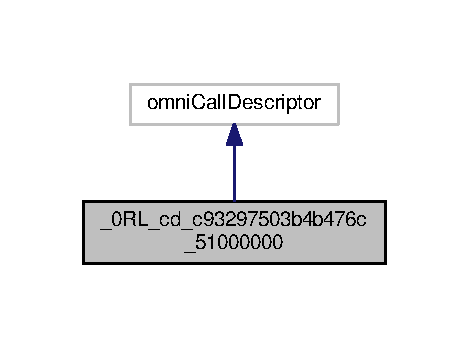
\includegraphics[width=225pt]{class__0_r_l__cd__c93297503b4b476c__51000000__inherit__graph}
\end{center}
\end{figure}


Collaboration diagram for \+\_\+0\+R\+L\+\_\+cd\+\_\+c93297503b4b476c\+\_\+51000000\+:
\nopagebreak
\begin{figure}[H]
\begin{center}
\leavevmode
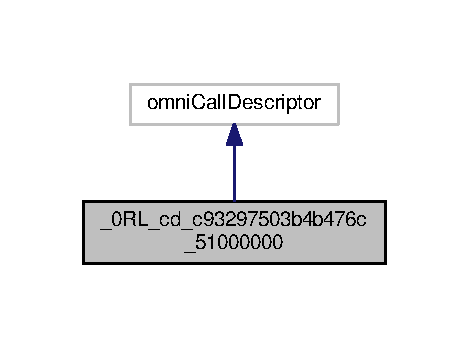
\includegraphics[width=225pt]{class__0_r_l__cd__c93297503b4b476c__51000000__coll__graph}
\end{center}
\end{figure}
\subsection*{Public Member Functions}
\begin{DoxyCompactItemize}
\item 
\hyperlink{class__0_r_l__cd__c93297503b4b476c__51000000_a6f7e0eae6f7801b77639a1abe8eb6b3c}{\+\_\+0\+R\+L\+\_\+cd\+\_\+c93297503b4b476c\+\_\+51000000} (Local\+Call\+Fn lcfn, const char $\ast$op\+\_\+, size\+\_\+t oplen, \+\_\+\+C\+O\+R\+B\+A\+\_\+\+Boolean upcall=0)
\item 
void \hyperlink{class__0_r_l__cd__c93297503b4b476c__51000000_adba2397575a650482c38d6373ef541bc}{marshal\+Arguments} (cdr\+Stream \&)
\item 
void \hyperlink{class__0_r_l__cd__c93297503b4b476c__51000000_ad28d04aa3e04b0339dfd32d5fc018071}{unmarshal\+Arguments} (cdr\+Stream \&)
\item 
void \hyperlink{class__0_r_l__cd__c93297503b4b476c__51000000_ad8ebd81f2bcb26aca9398a4c2f127430}{unmarshal\+Returned\+Values} (cdr\+Stream \&)
\item 
void \hyperlink{class__0_r_l__cd__c93297503b4b476c__51000000_ae44ad06ddf14be024d787efb55abb721}{marshal\+Returned\+Values} (cdr\+Stream \&)
\item 
void \hyperlink{class__0_r_l__cd__c93297503b4b476c__51000000_acd2879e7cb098e9b6d8d308f0dbe93d8}{user\+Exception} (cdr\+Stream \&, \+\_\+\+O\+M\+N\+I\+\_\+\+NS(I\+O\+P\+\_\+C)$\ast$, const char $\ast$)
\end{DoxyCompactItemize}
\subsection*{Public Attributes}
\begin{DoxyCompactItemize}
\item 
\+::C\+O\+R\+B\+A\+::\+String\+\_\+var \hyperlink{class__0_r_l__cd__c93297503b4b476c__51000000_ad86d0df67a8dfd4a7b88a247aebbfe67}{arg\+\_\+0\+\_\+}
\item 
const char $\ast$ \hyperlink{class__0_r_l__cd__c93297503b4b476c__51000000_a81e981035dd946f135928f6dbca1567f}{arg\+\_\+0}
\item 
Petit\+Prince\+::\+Point\+Seq\+\_\+var \hyperlink{class__0_r_l__cd__c93297503b4b476c__51000000_a20400a7189ab950f2440a9eff1293092}{arg\+\_\+1\+\_\+}
\item 
const Petit\+Prince\+::\+Point\+Seq $\ast$ \hyperlink{class__0_r_l__cd__c93297503b4b476c__51000000_a7a12cf2b92afccb92f38ae00be0d91d8}{arg\+\_\+1}
\item 
\+::C\+O\+R\+B\+A\+::\+Long \hyperlink{class__0_r_l__cd__c93297503b4b476c__51000000_a670d0d3e4c907d3c2a1e627ed061c956}{result}
\end{DoxyCompactItemize}
\subsection*{Static Public Attributes}
\begin{DoxyCompactItemize}
\item 
static const char $\ast$const \hyperlink{class__0_r_l__cd__c93297503b4b476c__51000000_a1b4142b3c9fdc007c834f3872ff72448}{\+\_\+user\+\_\+exns} \mbox{[}$\,$\mbox{]}
\end{DoxyCompactItemize}


\subsection{Detailed Description}


Definition at line 2257 of file Petit\+Prince\+\_\+\+Stub.\+cpp.



\subsection{Constructor \& Destructor Documentation}
\index{\+\_\+0\+R\+L\+\_\+cd\+\_\+c93297503b4b476c\+\_\+51000000@{\+\_\+0\+R\+L\+\_\+cd\+\_\+c93297503b4b476c\+\_\+51000000}!\+\_\+0\+R\+L\+\_\+cd\+\_\+c93297503b4b476c\+\_\+51000000@{\+\_\+0\+R\+L\+\_\+cd\+\_\+c93297503b4b476c\+\_\+51000000}}
\index{\+\_\+0\+R\+L\+\_\+cd\+\_\+c93297503b4b476c\+\_\+51000000@{\+\_\+0\+R\+L\+\_\+cd\+\_\+c93297503b4b476c\+\_\+51000000}!\+\_\+0\+R\+L\+\_\+cd\+\_\+c93297503b4b476c\+\_\+51000000@{\+\_\+0\+R\+L\+\_\+cd\+\_\+c93297503b4b476c\+\_\+51000000}}
\subsubsection[{\texorpdfstring{\+\_\+0\+R\+L\+\_\+cd\+\_\+c93297503b4b476c\+\_\+51000000(\+Local\+Call\+Fn lcfn, const char $\ast$op\+\_\+, size\+\_\+t oplen, \+\_\+\+C\+O\+R\+B\+A\+\_\+\+Boolean upcall=0)}{_0RL_cd_c93297503b4b476c_51000000(LocalCallFn lcfn, const char *op_, size_t oplen, _CORBA_Boolean upcall=0)}}]{\setlength{\rightskip}{0pt plus 5cm}\+\_\+0\+R\+L\+\_\+cd\+\_\+c93297503b4b476c\+\_\+51000000\+::\+\_\+0\+R\+L\+\_\+cd\+\_\+c93297503b4b476c\+\_\+51000000 (
\begin{DoxyParamCaption}
\item[{Local\+Call\+Fn}]{lcfn, }
\item[{const char $\ast$}]{op\+\_\+, }
\item[{size\+\_\+t}]{oplen, }
\item[{\+\_\+\+C\+O\+R\+B\+A\+\_\+\+Boolean}]{upcall = {\ttfamily 0}}
\end{DoxyParamCaption}
)\hspace{0.3cm}{\ttfamily [inline]}}\hypertarget{class__0_r_l__cd__c93297503b4b476c__51000000_a6f7e0eae6f7801b77639a1abe8eb6b3c}{}\label{class__0_r_l__cd__c93297503b4b476c__51000000_a6f7e0eae6f7801b77639a1abe8eb6b3c}


Definition at line 2261 of file Petit\+Prince\+\_\+\+Stub.\+cpp.



\subsection{Member Function Documentation}
\index{\+\_\+0\+R\+L\+\_\+cd\+\_\+c93297503b4b476c\+\_\+51000000@{\+\_\+0\+R\+L\+\_\+cd\+\_\+c93297503b4b476c\+\_\+51000000}!marshal\+Arguments@{marshal\+Arguments}}
\index{marshal\+Arguments@{marshal\+Arguments}!\+\_\+0\+R\+L\+\_\+cd\+\_\+c93297503b4b476c\+\_\+51000000@{\+\_\+0\+R\+L\+\_\+cd\+\_\+c93297503b4b476c\+\_\+51000000}}
\subsubsection[{\texorpdfstring{marshal\+Arguments(cdr\+Stream \&)}{marshalArguments(cdrStream &)}}]{\setlength{\rightskip}{0pt plus 5cm}void \+\_\+0\+R\+L\+\_\+cd\+\_\+c93297503b4b476c\+\_\+51000000\+::marshal\+Arguments (
\begin{DoxyParamCaption}
\item[{cdr\+Stream \&}]{\+\_\+n}
\end{DoxyParamCaption}
)}\hypertarget{class__0_r_l__cd__c93297503b4b476c__51000000_adba2397575a650482c38d6373ef541bc}{}\label{class__0_r_l__cd__c93297503b4b476c__51000000_adba2397575a650482c38d6373ef541bc}


Definition at line 2283 of file Petit\+Prince\+\_\+\+Stub.\+cpp.

\index{\+\_\+0\+R\+L\+\_\+cd\+\_\+c93297503b4b476c\+\_\+51000000@{\+\_\+0\+R\+L\+\_\+cd\+\_\+c93297503b4b476c\+\_\+51000000}!marshal\+Returned\+Values@{marshal\+Returned\+Values}}
\index{marshal\+Returned\+Values@{marshal\+Returned\+Values}!\+\_\+0\+R\+L\+\_\+cd\+\_\+c93297503b4b476c\+\_\+51000000@{\+\_\+0\+R\+L\+\_\+cd\+\_\+c93297503b4b476c\+\_\+51000000}}
\subsubsection[{\texorpdfstring{marshal\+Returned\+Values(cdr\+Stream \&)}{marshalReturnedValues(cdrStream &)}}]{\setlength{\rightskip}{0pt plus 5cm}void \+\_\+0\+R\+L\+\_\+cd\+\_\+c93297503b4b476c\+\_\+51000000\+::marshal\+Returned\+Values (
\begin{DoxyParamCaption}
\item[{cdr\+Stream \&}]{\+\_\+n}
\end{DoxyParamCaption}
)}\hypertarget{class__0_r_l__cd__c93297503b4b476c__51000000_ae44ad06ddf14be024d787efb55abb721}{}\label{class__0_r_l__cd__c93297503b4b476c__51000000_ae44ad06ddf14be024d787efb55abb721}


Definition at line 2300 of file Petit\+Prince\+\_\+\+Stub.\+cpp.

\index{\+\_\+0\+R\+L\+\_\+cd\+\_\+c93297503b4b476c\+\_\+51000000@{\+\_\+0\+R\+L\+\_\+cd\+\_\+c93297503b4b476c\+\_\+51000000}!unmarshal\+Arguments@{unmarshal\+Arguments}}
\index{unmarshal\+Arguments@{unmarshal\+Arguments}!\+\_\+0\+R\+L\+\_\+cd\+\_\+c93297503b4b476c\+\_\+51000000@{\+\_\+0\+R\+L\+\_\+cd\+\_\+c93297503b4b476c\+\_\+51000000}}
\subsubsection[{\texorpdfstring{unmarshal\+Arguments(cdr\+Stream \&)}{unmarshalArguments(cdrStream &)}}]{\setlength{\rightskip}{0pt plus 5cm}void \+\_\+0\+R\+L\+\_\+cd\+\_\+c93297503b4b476c\+\_\+51000000\+::unmarshal\+Arguments (
\begin{DoxyParamCaption}
\item[{cdr\+Stream \&}]{\+\_\+n}
\end{DoxyParamCaption}
)}\hypertarget{class__0_r_l__cd__c93297503b4b476c__51000000_ad28d04aa3e04b0339dfd32d5fc018071}{}\label{class__0_r_l__cd__c93297503b4b476c__51000000_ad28d04aa3e04b0339dfd32d5fc018071}


Definition at line 2290 of file Petit\+Prince\+\_\+\+Stub.\+cpp.

\index{\+\_\+0\+R\+L\+\_\+cd\+\_\+c93297503b4b476c\+\_\+51000000@{\+\_\+0\+R\+L\+\_\+cd\+\_\+c93297503b4b476c\+\_\+51000000}!unmarshal\+Returned\+Values@{unmarshal\+Returned\+Values}}
\index{unmarshal\+Returned\+Values@{unmarshal\+Returned\+Values}!\+\_\+0\+R\+L\+\_\+cd\+\_\+c93297503b4b476c\+\_\+51000000@{\+\_\+0\+R\+L\+\_\+cd\+\_\+c93297503b4b476c\+\_\+51000000}}
\subsubsection[{\texorpdfstring{unmarshal\+Returned\+Values(cdr\+Stream \&)}{unmarshalReturnedValues(cdrStream &)}}]{\setlength{\rightskip}{0pt plus 5cm}void \+\_\+0\+R\+L\+\_\+cd\+\_\+c93297503b4b476c\+\_\+51000000\+::unmarshal\+Returned\+Values (
\begin{DoxyParamCaption}
\item[{cdr\+Stream \&}]{\+\_\+n}
\end{DoxyParamCaption}
)}\hypertarget{class__0_r_l__cd__c93297503b4b476c__51000000_ad8ebd81f2bcb26aca9398a4c2f127430}{}\label{class__0_r_l__cd__c93297503b4b476c__51000000_ad8ebd81f2bcb26aca9398a4c2f127430}


Definition at line 2306 of file Petit\+Prince\+\_\+\+Stub.\+cpp.

\index{\+\_\+0\+R\+L\+\_\+cd\+\_\+c93297503b4b476c\+\_\+51000000@{\+\_\+0\+R\+L\+\_\+cd\+\_\+c93297503b4b476c\+\_\+51000000}!user\+Exception@{user\+Exception}}
\index{user\+Exception@{user\+Exception}!\+\_\+0\+R\+L\+\_\+cd\+\_\+c93297503b4b476c\+\_\+51000000@{\+\_\+0\+R\+L\+\_\+cd\+\_\+c93297503b4b476c\+\_\+51000000}}
\subsubsection[{\texorpdfstring{user\+Exception(cdr\+Stream \&, \+\_\+\+O\+M\+N\+I\+\_\+\+N\+S(\+I\+O\+P\+\_\+\+C)$\ast$, const char $\ast$)}{userException(cdrStream &, _OMNI_NS(IOP_C)*, const char *)}}]{\setlength{\rightskip}{0pt plus 5cm}void \+\_\+0\+R\+L\+\_\+cd\+\_\+c93297503b4b476c\+\_\+51000000\+::user\+Exception (
\begin{DoxyParamCaption}
\item[{cdr\+Stream \&}]{s, }
\item[{\+\_\+\+O\+M\+N\+I\+\_\+\+NS(I\+O\+P\+\_\+C)$\ast$}]{iop\+\_\+client, }
\item[{const char $\ast$}]{repo\+Id}
\end{DoxyParamCaption}
)}\hypertarget{class__0_r_l__cd__c93297503b4b476c__51000000_acd2879e7cb098e9b6d8d308f0dbe93d8}{}\label{class__0_r_l__cd__c93297503b4b476c__51000000_acd2879e7cb098e9b6d8d308f0dbe93d8}


Definition at line 2316 of file Petit\+Prince\+\_\+\+Stub.\+cpp.



\subsection{Member Data Documentation}
\index{\+\_\+0\+R\+L\+\_\+cd\+\_\+c93297503b4b476c\+\_\+51000000@{\+\_\+0\+R\+L\+\_\+cd\+\_\+c93297503b4b476c\+\_\+51000000}!\+\_\+user\+\_\+exns@{\+\_\+user\+\_\+exns}}
\index{\+\_\+user\+\_\+exns@{\+\_\+user\+\_\+exns}!\+\_\+0\+R\+L\+\_\+cd\+\_\+c93297503b4b476c\+\_\+51000000@{\+\_\+0\+R\+L\+\_\+cd\+\_\+c93297503b4b476c\+\_\+51000000}}
\subsubsection[{\texorpdfstring{\+\_\+user\+\_\+exns}{_user_exns}}]{\setlength{\rightskip}{0pt plus 5cm}const char $\ast$const \+\_\+0\+R\+L\+\_\+cd\+\_\+c93297503b4b476c\+\_\+51000000\+::\+\_\+user\+\_\+exns\hspace{0.3cm}{\ttfamily [static]}}\hypertarget{class__0_r_l__cd__c93297503b4b476c__51000000_a1b4142b3c9fdc007c834f3872ff72448}{}\label{class__0_r_l__cd__c93297503b4b476c__51000000_a1b4142b3c9fdc007c834f3872ff72448}
{\bfseries Initial value\+:}
\begin{DoxyCode}
= \{
  PetitPrince::PetitPrinceService::InvalidDrawParams::\_PD\_repoId
\}
\end{DoxyCode}


Definition at line 2274 of file Petit\+Prince\+\_\+\+Stub.\+cpp.

\index{\+\_\+0\+R\+L\+\_\+cd\+\_\+c93297503b4b476c\+\_\+51000000@{\+\_\+0\+R\+L\+\_\+cd\+\_\+c93297503b4b476c\+\_\+51000000}!arg\+\_\+0@{arg\+\_\+0}}
\index{arg\+\_\+0@{arg\+\_\+0}!\+\_\+0\+R\+L\+\_\+cd\+\_\+c93297503b4b476c\+\_\+51000000@{\+\_\+0\+R\+L\+\_\+cd\+\_\+c93297503b4b476c\+\_\+51000000}}
\subsubsection[{\texorpdfstring{arg\+\_\+0}{arg_0}}]{\setlength{\rightskip}{0pt plus 5cm}const char$\ast$ \+\_\+0\+R\+L\+\_\+cd\+\_\+c93297503b4b476c\+\_\+51000000\+::arg\+\_\+0}\hypertarget{class__0_r_l__cd__c93297503b4b476c__51000000_a81e981035dd946f135928f6dbca1567f}{}\label{class__0_r_l__cd__c93297503b4b476c__51000000_a81e981035dd946f135928f6dbca1567f}


Definition at line 2277 of file Petit\+Prince\+\_\+\+Stub.\+cpp.

\index{\+\_\+0\+R\+L\+\_\+cd\+\_\+c93297503b4b476c\+\_\+51000000@{\+\_\+0\+R\+L\+\_\+cd\+\_\+c93297503b4b476c\+\_\+51000000}!arg\+\_\+0\+\_\+@{arg\+\_\+0\+\_\+}}
\index{arg\+\_\+0\+\_\+@{arg\+\_\+0\+\_\+}!\+\_\+0\+R\+L\+\_\+cd\+\_\+c93297503b4b476c\+\_\+51000000@{\+\_\+0\+R\+L\+\_\+cd\+\_\+c93297503b4b476c\+\_\+51000000}}
\subsubsection[{\texorpdfstring{arg\+\_\+0\+\_\+}{arg_0_}}]{\setlength{\rightskip}{0pt plus 5cm}\+::C\+O\+R\+B\+A\+::\+String\+\_\+var \+\_\+0\+R\+L\+\_\+cd\+\_\+c93297503b4b476c\+\_\+51000000\+::arg\+\_\+0\+\_\+}\hypertarget{class__0_r_l__cd__c93297503b4b476c__51000000_ad86d0df67a8dfd4a7b88a247aebbfe67}{}\label{class__0_r_l__cd__c93297503b4b476c__51000000_ad86d0df67a8dfd4a7b88a247aebbfe67}


Definition at line 2276 of file Petit\+Prince\+\_\+\+Stub.\+cpp.

\index{\+\_\+0\+R\+L\+\_\+cd\+\_\+c93297503b4b476c\+\_\+51000000@{\+\_\+0\+R\+L\+\_\+cd\+\_\+c93297503b4b476c\+\_\+51000000}!arg\+\_\+1@{arg\+\_\+1}}
\index{arg\+\_\+1@{arg\+\_\+1}!\+\_\+0\+R\+L\+\_\+cd\+\_\+c93297503b4b476c\+\_\+51000000@{\+\_\+0\+R\+L\+\_\+cd\+\_\+c93297503b4b476c\+\_\+51000000}}
\subsubsection[{\texorpdfstring{arg\+\_\+1}{arg_1}}]{\setlength{\rightskip}{0pt plus 5cm}const Petit\+Prince\+::\+Point\+Seq$\ast$ \+\_\+0\+R\+L\+\_\+cd\+\_\+c93297503b4b476c\+\_\+51000000\+::arg\+\_\+1}\hypertarget{class__0_r_l__cd__c93297503b4b476c__51000000_a7a12cf2b92afccb92f38ae00be0d91d8}{}\label{class__0_r_l__cd__c93297503b4b476c__51000000_a7a12cf2b92afccb92f38ae00be0d91d8}


Definition at line 2279 of file Petit\+Prince\+\_\+\+Stub.\+cpp.

\index{\+\_\+0\+R\+L\+\_\+cd\+\_\+c93297503b4b476c\+\_\+51000000@{\+\_\+0\+R\+L\+\_\+cd\+\_\+c93297503b4b476c\+\_\+51000000}!arg\+\_\+1\+\_\+@{arg\+\_\+1\+\_\+}}
\index{arg\+\_\+1\+\_\+@{arg\+\_\+1\+\_\+}!\+\_\+0\+R\+L\+\_\+cd\+\_\+c93297503b4b476c\+\_\+51000000@{\+\_\+0\+R\+L\+\_\+cd\+\_\+c93297503b4b476c\+\_\+51000000}}
\subsubsection[{\texorpdfstring{arg\+\_\+1\+\_\+}{arg_1_}}]{\setlength{\rightskip}{0pt plus 5cm}Petit\+Prince\+::\+Point\+Seq\+\_\+var \+\_\+0\+R\+L\+\_\+cd\+\_\+c93297503b4b476c\+\_\+51000000\+::arg\+\_\+1\+\_\+}\hypertarget{class__0_r_l__cd__c93297503b4b476c__51000000_a20400a7189ab950f2440a9eff1293092}{}\label{class__0_r_l__cd__c93297503b4b476c__51000000_a20400a7189ab950f2440a9eff1293092}


Definition at line 2278 of file Petit\+Prince\+\_\+\+Stub.\+cpp.

\index{\+\_\+0\+R\+L\+\_\+cd\+\_\+c93297503b4b476c\+\_\+51000000@{\+\_\+0\+R\+L\+\_\+cd\+\_\+c93297503b4b476c\+\_\+51000000}!result@{result}}
\index{result@{result}!\+\_\+0\+R\+L\+\_\+cd\+\_\+c93297503b4b476c\+\_\+51000000@{\+\_\+0\+R\+L\+\_\+cd\+\_\+c93297503b4b476c\+\_\+51000000}}
\subsubsection[{\texorpdfstring{result}{result}}]{\setlength{\rightskip}{0pt plus 5cm}\+::C\+O\+R\+B\+A\+::\+Long \+\_\+0\+R\+L\+\_\+cd\+\_\+c93297503b4b476c\+\_\+51000000\+::result}\hypertarget{class__0_r_l__cd__c93297503b4b476c__51000000_a670d0d3e4c907d3c2a1e627ed061c956}{}\label{class__0_r_l__cd__c93297503b4b476c__51000000_a670d0d3e4c907d3c2a1e627ed061c956}


Definition at line 2280 of file Petit\+Prince\+\_\+\+Stub.\+cpp.



The documentation for this class was generated from the following file\+:\begin{DoxyCompactItemize}
\item 
src/\hyperlink{_petit_prince___stub_8cpp}{Petit\+Prince\+\_\+\+Stub.\+cpp}\end{DoxyCompactItemize}

\hypertarget{class__0_r_l__cd__c93297503b4b476c__71000000}{}\section{\+\_\+0\+R\+L\+\_\+cd\+\_\+c93297503b4b476c\+\_\+71000000 Class Reference}
\label{class__0_r_l__cd__c93297503b4b476c__71000000}\index{\+\_\+0\+R\+L\+\_\+cd\+\_\+c93297503b4b476c\+\_\+71000000@{\+\_\+0\+R\+L\+\_\+cd\+\_\+c93297503b4b476c\+\_\+71000000}}


Inheritance diagram for \+\_\+0\+R\+L\+\_\+cd\+\_\+c93297503b4b476c\+\_\+71000000\+:
\nopagebreak
\begin{figure}[H]
\begin{center}
\leavevmode
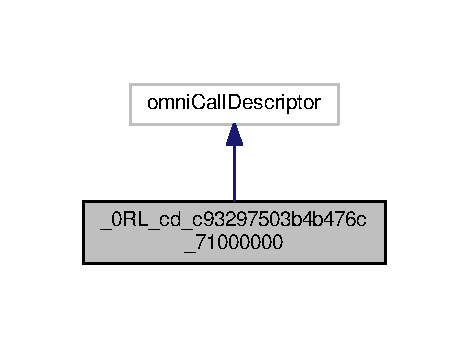
\includegraphics[width=225pt]{class__0_r_l__cd__c93297503b4b476c__71000000__inherit__graph}
\end{center}
\end{figure}


Collaboration diagram for \+\_\+0\+R\+L\+\_\+cd\+\_\+c93297503b4b476c\+\_\+71000000\+:
\nopagebreak
\begin{figure}[H]
\begin{center}
\leavevmode
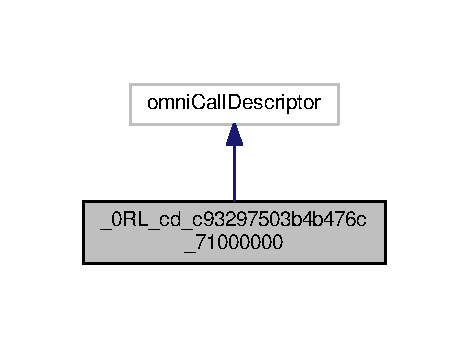
\includegraphics[width=225pt]{class__0_r_l__cd__c93297503b4b476c__71000000__coll__graph}
\end{center}
\end{figure}
\subsection*{Public Member Functions}
\begin{DoxyCompactItemize}
\item 
\hyperlink{class__0_r_l__cd__c93297503b4b476c__71000000_ae711a0879586fbc0bccb6887b7fc7bff}{\+\_\+0\+R\+L\+\_\+cd\+\_\+c93297503b4b476c\+\_\+71000000} (Local\+Call\+Fn lcfn, const char $\ast$op\+\_\+, size\+\_\+t oplen, \+\_\+\+C\+O\+R\+B\+A\+\_\+\+Boolean upcall=0)
\item 
void \hyperlink{class__0_r_l__cd__c93297503b4b476c__71000000_a3839819b898206d349b14e6b4aa4a74a}{marshal\+Arguments} (cdr\+Stream \&)
\item 
void \hyperlink{class__0_r_l__cd__c93297503b4b476c__71000000_ac438529ffd9dabbf8e353a1e38de57ea}{unmarshal\+Arguments} (cdr\+Stream \&)
\item 
void \hyperlink{class__0_r_l__cd__c93297503b4b476c__71000000_a4006a83ad5a5c7e5edd51341cd8c6324}{unmarshal\+Returned\+Values} (cdr\+Stream \&)
\item 
void \hyperlink{class__0_r_l__cd__c93297503b4b476c__71000000_a1c622901175edcd45e3f5144a98b55ee}{marshal\+Returned\+Values} (cdr\+Stream \&)
\end{DoxyCompactItemize}
\subsection*{Public Attributes}
\begin{DoxyCompactItemize}
\item 
\+::C\+O\+R\+B\+A\+::\+String\+\_\+var \hyperlink{class__0_r_l__cd__c93297503b4b476c__71000000_a6c99db7522f081f5f960329aa52f2939}{arg\+\_\+0\+\_\+}
\item 
const char $\ast$ \hyperlink{class__0_r_l__cd__c93297503b4b476c__71000000_a39f171638e7d97e43ebabca56ce6f925}{arg\+\_\+0}
\item 
Petit\+Prince\+::\+Long\+Seq\+\_\+var \hyperlink{class__0_r_l__cd__c93297503b4b476c__71000000_af3a56f469452c58aa0b15ff954198b07}{result}
\end{DoxyCompactItemize}
\subsection*{Static Public Attributes}
\begin{DoxyCompactItemize}
\item 
static const char $\ast$const \hyperlink{class__0_r_l__cd__c93297503b4b476c__71000000_a9041720817a437b67d07c1b7ac18c903}{\+\_\+user\+\_\+exns} \mbox{[}$\,$\mbox{]}
\end{DoxyCompactItemize}


\subsection{Detailed Description}


Definition at line 2372 of file Petit\+Prince\+\_\+\+Stub.\+cpp.



\subsection{Constructor \& Destructor Documentation}
\index{\+\_\+0\+R\+L\+\_\+cd\+\_\+c93297503b4b476c\+\_\+71000000@{\+\_\+0\+R\+L\+\_\+cd\+\_\+c93297503b4b476c\+\_\+71000000}!\+\_\+0\+R\+L\+\_\+cd\+\_\+c93297503b4b476c\+\_\+71000000@{\+\_\+0\+R\+L\+\_\+cd\+\_\+c93297503b4b476c\+\_\+71000000}}
\index{\+\_\+0\+R\+L\+\_\+cd\+\_\+c93297503b4b476c\+\_\+71000000@{\+\_\+0\+R\+L\+\_\+cd\+\_\+c93297503b4b476c\+\_\+71000000}!\+\_\+0\+R\+L\+\_\+cd\+\_\+c93297503b4b476c\+\_\+71000000@{\+\_\+0\+R\+L\+\_\+cd\+\_\+c93297503b4b476c\+\_\+71000000}}
\subsubsection[{\texorpdfstring{\+\_\+0\+R\+L\+\_\+cd\+\_\+c93297503b4b476c\+\_\+71000000(\+Local\+Call\+Fn lcfn, const char $\ast$op\+\_\+, size\+\_\+t oplen, \+\_\+\+C\+O\+R\+B\+A\+\_\+\+Boolean upcall=0)}{_0RL_cd_c93297503b4b476c_71000000(LocalCallFn lcfn, const char *op_, size_t oplen, _CORBA_Boolean upcall=0)}}]{\setlength{\rightskip}{0pt plus 5cm}\+\_\+0\+R\+L\+\_\+cd\+\_\+c93297503b4b476c\+\_\+71000000\+::\+\_\+0\+R\+L\+\_\+cd\+\_\+c93297503b4b476c\+\_\+71000000 (
\begin{DoxyParamCaption}
\item[{Local\+Call\+Fn}]{lcfn, }
\item[{const char $\ast$}]{op\+\_\+, }
\item[{size\+\_\+t}]{oplen, }
\item[{\+\_\+\+C\+O\+R\+B\+A\+\_\+\+Boolean}]{upcall = {\ttfamily 0}}
\end{DoxyParamCaption}
)\hspace{0.3cm}{\ttfamily [inline]}}\hypertarget{class__0_r_l__cd__c93297503b4b476c__71000000_ae711a0879586fbc0bccb6887b7fc7bff}{}\label{class__0_r_l__cd__c93297503b4b476c__71000000_ae711a0879586fbc0bccb6887b7fc7bff}


Definition at line 2376 of file Petit\+Prince\+\_\+\+Stub.\+cpp.



\subsection{Member Function Documentation}
\index{\+\_\+0\+R\+L\+\_\+cd\+\_\+c93297503b4b476c\+\_\+71000000@{\+\_\+0\+R\+L\+\_\+cd\+\_\+c93297503b4b476c\+\_\+71000000}!marshal\+Arguments@{marshal\+Arguments}}
\index{marshal\+Arguments@{marshal\+Arguments}!\+\_\+0\+R\+L\+\_\+cd\+\_\+c93297503b4b476c\+\_\+71000000@{\+\_\+0\+R\+L\+\_\+cd\+\_\+c93297503b4b476c\+\_\+71000000}}
\subsubsection[{\texorpdfstring{marshal\+Arguments(cdr\+Stream \&)}{marshalArguments(cdrStream &)}}]{\setlength{\rightskip}{0pt plus 5cm}void \+\_\+0\+R\+L\+\_\+cd\+\_\+c93297503b4b476c\+\_\+71000000\+::marshal\+Arguments (
\begin{DoxyParamCaption}
\item[{cdr\+Stream \&}]{\+\_\+n}
\end{DoxyParamCaption}
)}\hypertarget{class__0_r_l__cd__c93297503b4b476c__71000000_a3839819b898206d349b14e6b4aa4a74a}{}\label{class__0_r_l__cd__c93297503b4b476c__71000000_a3839819b898206d349b14e6b4aa4a74a}


Definition at line 2396 of file Petit\+Prince\+\_\+\+Stub.\+cpp.

\index{\+\_\+0\+R\+L\+\_\+cd\+\_\+c93297503b4b476c\+\_\+71000000@{\+\_\+0\+R\+L\+\_\+cd\+\_\+c93297503b4b476c\+\_\+71000000}!marshal\+Returned\+Values@{marshal\+Returned\+Values}}
\index{marshal\+Returned\+Values@{marshal\+Returned\+Values}!\+\_\+0\+R\+L\+\_\+cd\+\_\+c93297503b4b476c\+\_\+71000000@{\+\_\+0\+R\+L\+\_\+cd\+\_\+c93297503b4b476c\+\_\+71000000}}
\subsubsection[{\texorpdfstring{marshal\+Returned\+Values(cdr\+Stream \&)}{marshalReturnedValues(cdrStream &)}}]{\setlength{\rightskip}{0pt plus 5cm}void \+\_\+0\+R\+L\+\_\+cd\+\_\+c93297503b4b476c\+\_\+71000000\+::marshal\+Returned\+Values (
\begin{DoxyParamCaption}
\item[{cdr\+Stream \&}]{\+\_\+n}
\end{DoxyParamCaption}
)}\hypertarget{class__0_r_l__cd__c93297503b4b476c__71000000_a1c622901175edcd45e3f5144a98b55ee}{}\label{class__0_r_l__cd__c93297503b4b476c__71000000_a1c622901175edcd45e3f5144a98b55ee}


Definition at line 2409 of file Petit\+Prince\+\_\+\+Stub.\+cpp.

\index{\+\_\+0\+R\+L\+\_\+cd\+\_\+c93297503b4b476c\+\_\+71000000@{\+\_\+0\+R\+L\+\_\+cd\+\_\+c93297503b4b476c\+\_\+71000000}!unmarshal\+Arguments@{unmarshal\+Arguments}}
\index{unmarshal\+Arguments@{unmarshal\+Arguments}!\+\_\+0\+R\+L\+\_\+cd\+\_\+c93297503b4b476c\+\_\+71000000@{\+\_\+0\+R\+L\+\_\+cd\+\_\+c93297503b4b476c\+\_\+71000000}}
\subsubsection[{\texorpdfstring{unmarshal\+Arguments(cdr\+Stream \&)}{unmarshalArguments(cdrStream &)}}]{\setlength{\rightskip}{0pt plus 5cm}void \+\_\+0\+R\+L\+\_\+cd\+\_\+c93297503b4b476c\+\_\+71000000\+::unmarshal\+Arguments (
\begin{DoxyParamCaption}
\item[{cdr\+Stream \&}]{\+\_\+n}
\end{DoxyParamCaption}
)}\hypertarget{class__0_r_l__cd__c93297503b4b476c__71000000_ac438529ffd9dabbf8e353a1e38de57ea}{}\label{class__0_r_l__cd__c93297503b4b476c__71000000_ac438529ffd9dabbf8e353a1e38de57ea}


Definition at line 2402 of file Petit\+Prince\+\_\+\+Stub.\+cpp.

\index{\+\_\+0\+R\+L\+\_\+cd\+\_\+c93297503b4b476c\+\_\+71000000@{\+\_\+0\+R\+L\+\_\+cd\+\_\+c93297503b4b476c\+\_\+71000000}!unmarshal\+Returned\+Values@{unmarshal\+Returned\+Values}}
\index{unmarshal\+Returned\+Values@{unmarshal\+Returned\+Values}!\+\_\+0\+R\+L\+\_\+cd\+\_\+c93297503b4b476c\+\_\+71000000@{\+\_\+0\+R\+L\+\_\+cd\+\_\+c93297503b4b476c\+\_\+71000000}}
\subsubsection[{\texorpdfstring{unmarshal\+Returned\+Values(cdr\+Stream \&)}{unmarshalReturnedValues(cdrStream &)}}]{\setlength{\rightskip}{0pt plus 5cm}void \+\_\+0\+R\+L\+\_\+cd\+\_\+c93297503b4b476c\+\_\+71000000\+::unmarshal\+Returned\+Values (
\begin{DoxyParamCaption}
\item[{cdr\+Stream \&}]{\+\_\+n}
\end{DoxyParamCaption}
)}\hypertarget{class__0_r_l__cd__c93297503b4b476c__71000000_a4006a83ad5a5c7e5edd51341cd8c6324}{}\label{class__0_r_l__cd__c93297503b4b476c__71000000_a4006a83ad5a5c7e5edd51341cd8c6324}


Definition at line 2415 of file Petit\+Prince\+\_\+\+Stub.\+cpp.



\subsection{Member Data Documentation}
\index{\+\_\+0\+R\+L\+\_\+cd\+\_\+c93297503b4b476c\+\_\+71000000@{\+\_\+0\+R\+L\+\_\+cd\+\_\+c93297503b4b476c\+\_\+71000000}!\+\_\+user\+\_\+exns@{\+\_\+user\+\_\+exns}}
\index{\+\_\+user\+\_\+exns@{\+\_\+user\+\_\+exns}!\+\_\+0\+R\+L\+\_\+cd\+\_\+c93297503b4b476c\+\_\+71000000@{\+\_\+0\+R\+L\+\_\+cd\+\_\+c93297503b4b476c\+\_\+71000000}}
\subsubsection[{\texorpdfstring{\+\_\+user\+\_\+exns}{_user_exns}}]{\setlength{\rightskip}{0pt plus 5cm}const char $\ast$const \+\_\+0\+R\+L\+\_\+cd\+\_\+c93297503b4b476c\+\_\+71000000\+::\+\_\+user\+\_\+exns\hspace{0.3cm}{\ttfamily [static]}}\hypertarget{class__0_r_l__cd__c93297503b4b476c__71000000_a9041720817a437b67d07c1b7ac18c903}{}\label{class__0_r_l__cd__c93297503b4b476c__71000000_a9041720817a437b67d07c1b7ac18c903}
{\bfseries Initial value\+:}
\begin{DoxyCode}
= \{
  0
\}
\end{DoxyCode}


Definition at line 2389 of file Petit\+Prince\+\_\+\+Stub.\+cpp.

\index{\+\_\+0\+R\+L\+\_\+cd\+\_\+c93297503b4b476c\+\_\+71000000@{\+\_\+0\+R\+L\+\_\+cd\+\_\+c93297503b4b476c\+\_\+71000000}!arg\+\_\+0@{arg\+\_\+0}}
\index{arg\+\_\+0@{arg\+\_\+0}!\+\_\+0\+R\+L\+\_\+cd\+\_\+c93297503b4b476c\+\_\+71000000@{\+\_\+0\+R\+L\+\_\+cd\+\_\+c93297503b4b476c\+\_\+71000000}}
\subsubsection[{\texorpdfstring{arg\+\_\+0}{arg_0}}]{\setlength{\rightskip}{0pt plus 5cm}const char$\ast$ \+\_\+0\+R\+L\+\_\+cd\+\_\+c93297503b4b476c\+\_\+71000000\+::arg\+\_\+0}\hypertarget{class__0_r_l__cd__c93297503b4b476c__71000000_a39f171638e7d97e43ebabca56ce6f925}{}\label{class__0_r_l__cd__c93297503b4b476c__71000000_a39f171638e7d97e43ebabca56ce6f925}


Definition at line 2392 of file Petit\+Prince\+\_\+\+Stub.\+cpp.

\index{\+\_\+0\+R\+L\+\_\+cd\+\_\+c93297503b4b476c\+\_\+71000000@{\+\_\+0\+R\+L\+\_\+cd\+\_\+c93297503b4b476c\+\_\+71000000}!arg\+\_\+0\+\_\+@{arg\+\_\+0\+\_\+}}
\index{arg\+\_\+0\+\_\+@{arg\+\_\+0\+\_\+}!\+\_\+0\+R\+L\+\_\+cd\+\_\+c93297503b4b476c\+\_\+71000000@{\+\_\+0\+R\+L\+\_\+cd\+\_\+c93297503b4b476c\+\_\+71000000}}
\subsubsection[{\texorpdfstring{arg\+\_\+0\+\_\+}{arg_0_}}]{\setlength{\rightskip}{0pt plus 5cm}\+::C\+O\+R\+B\+A\+::\+String\+\_\+var \+\_\+0\+R\+L\+\_\+cd\+\_\+c93297503b4b476c\+\_\+71000000\+::arg\+\_\+0\+\_\+}\hypertarget{class__0_r_l__cd__c93297503b4b476c__71000000_a6c99db7522f081f5f960329aa52f2939}{}\label{class__0_r_l__cd__c93297503b4b476c__71000000_a6c99db7522f081f5f960329aa52f2939}


Definition at line 2391 of file Petit\+Prince\+\_\+\+Stub.\+cpp.

\index{\+\_\+0\+R\+L\+\_\+cd\+\_\+c93297503b4b476c\+\_\+71000000@{\+\_\+0\+R\+L\+\_\+cd\+\_\+c93297503b4b476c\+\_\+71000000}!result@{result}}
\index{result@{result}!\+\_\+0\+R\+L\+\_\+cd\+\_\+c93297503b4b476c\+\_\+71000000@{\+\_\+0\+R\+L\+\_\+cd\+\_\+c93297503b4b476c\+\_\+71000000}}
\subsubsection[{\texorpdfstring{result}{result}}]{\setlength{\rightskip}{0pt plus 5cm}Petit\+Prince\+::\+Long\+Seq\+\_\+var \+\_\+0\+R\+L\+\_\+cd\+\_\+c93297503b4b476c\+\_\+71000000\+::result}\hypertarget{class__0_r_l__cd__c93297503b4b476c__71000000_af3a56f469452c58aa0b15ff954198b07}{}\label{class__0_r_l__cd__c93297503b4b476c__71000000_af3a56f469452c58aa0b15ff954198b07}


Definition at line 2393 of file Petit\+Prince\+\_\+\+Stub.\+cpp.



The documentation for this class was generated from the following file\+:\begin{DoxyCompactItemize}
\item 
src/\hyperlink{_petit_prince___stub_8cpp}{Petit\+Prince\+\_\+\+Stub.\+cpp}\end{DoxyCompactItemize}

\hypertarget{class__0_r_l__cd__c93297503b4b476c__80000000}{}\section{\+\_\+0\+R\+L\+\_\+cd\+\_\+c93297503b4b476c\+\_\+80000000 Class Reference}
\label{class__0_r_l__cd__c93297503b4b476c__80000000}\index{\+\_\+0\+R\+L\+\_\+cd\+\_\+c93297503b4b476c\+\_\+80000000@{\+\_\+0\+R\+L\+\_\+cd\+\_\+c93297503b4b476c\+\_\+80000000}}


Inheritance diagram for \+\_\+0\+R\+L\+\_\+cd\+\_\+c93297503b4b476c\+\_\+80000000\+:
\nopagebreak
\begin{figure}[H]
\begin{center}
\leavevmode
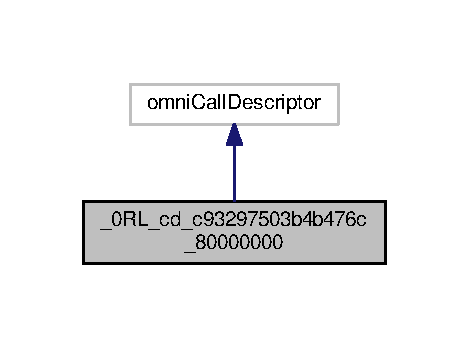
\includegraphics[width=225pt]{class__0_r_l__cd__c93297503b4b476c__80000000__inherit__graph}
\end{center}
\end{figure}


Collaboration diagram for \+\_\+0\+R\+L\+\_\+cd\+\_\+c93297503b4b476c\+\_\+80000000\+:
\nopagebreak
\begin{figure}[H]
\begin{center}
\leavevmode
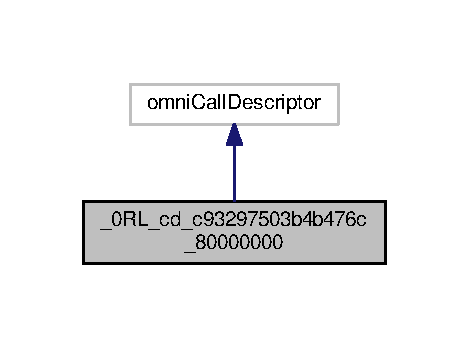
\includegraphics[width=225pt]{class__0_r_l__cd__c93297503b4b476c__80000000__coll__graph}
\end{center}
\end{figure}
\subsection*{Public Member Functions}
\begin{DoxyCompactItemize}
\item 
\hyperlink{class__0_r_l__cd__c93297503b4b476c__80000000_ad308c310fa659020a5700f1b678304ed}{\+\_\+0\+R\+L\+\_\+cd\+\_\+c93297503b4b476c\+\_\+80000000} (Local\+Call\+Fn lcfn, const char $\ast$op\+\_\+, size\+\_\+t oplen, \+\_\+\+C\+O\+R\+B\+A\+\_\+\+Boolean upcall=0)
\item 
void \hyperlink{class__0_r_l__cd__c93297503b4b476c__80000000_a4407e26307e25abe6ac90f6d213a27de}{marshal\+Arguments} (cdr\+Stream \&)
\item 
void \hyperlink{class__0_r_l__cd__c93297503b4b476c__80000000_a676d81c8b60993025cc6aca345e10ef3}{unmarshal\+Arguments} (cdr\+Stream \&)
\end{DoxyCompactItemize}
\subsection*{Public Attributes}
\begin{DoxyCompactItemize}
\item 
\+::C\+O\+R\+B\+A\+::\+Long \hyperlink{class__0_r_l__cd__c93297503b4b476c__80000000_a4c028c6d9f97e31f6f1c2daea15de53d}{arg\+\_\+0}
\end{DoxyCompactItemize}
\subsection*{Static Public Attributes}
\begin{DoxyCompactItemize}
\item 
static const char $\ast$const \hyperlink{class__0_r_l__cd__c93297503b4b476c__80000000_a7f9774a33ed16a3fa01df1cefaf8fcb4}{\+\_\+user\+\_\+exns} \mbox{[}$\,$\mbox{]}
\end{DoxyCompactItemize}


\subsection{Constructor \& Destructor Documentation}
\index{\+\_\+0\+R\+L\+\_\+cd\+\_\+c93297503b4b476c\+\_\+80000000@{\+\_\+0\+R\+L\+\_\+cd\+\_\+c93297503b4b476c\+\_\+80000000}!\+\_\+0\+R\+L\+\_\+cd\+\_\+c93297503b4b476c\+\_\+80000000@{\+\_\+0\+R\+L\+\_\+cd\+\_\+c93297503b4b476c\+\_\+80000000}}
\index{\+\_\+0\+R\+L\+\_\+cd\+\_\+c93297503b4b476c\+\_\+80000000@{\+\_\+0\+R\+L\+\_\+cd\+\_\+c93297503b4b476c\+\_\+80000000}!\+\_\+0\+R\+L\+\_\+cd\+\_\+c93297503b4b476c\+\_\+80000000@{\+\_\+0\+R\+L\+\_\+cd\+\_\+c93297503b4b476c\+\_\+80000000}}
\subsubsection[{\texorpdfstring{\+\_\+0\+R\+L\+\_\+cd\+\_\+c93297503b4b476c\+\_\+80000000(\+Local\+Call\+Fn lcfn, const char $\ast$op\+\_\+, size\+\_\+t oplen, \+\_\+\+C\+O\+R\+B\+A\+\_\+\+Boolean upcall=0)}{_0RL_cd_c93297503b4b476c_80000000(LocalCallFn lcfn, const char *op_, size_t oplen, _CORBA_Boolean upcall=0)}}]{\setlength{\rightskip}{0pt plus 5cm}\+\_\+0\+R\+L\+\_\+cd\+\_\+c93297503b4b476c\+\_\+80000000\+::\+\_\+0\+R\+L\+\_\+cd\+\_\+c93297503b4b476c\+\_\+80000000 (
\begin{DoxyParamCaption}
\item[{Local\+Call\+Fn}]{lcfn, }
\item[{const char $\ast$}]{op\+\_\+, }
\item[{size\+\_\+t}]{oplen, }
\item[{\+\_\+\+C\+O\+R\+B\+A\+\_\+\+Boolean}]{upcall = {\ttfamily 0}}
\end{DoxyParamCaption}
)\hspace{0.3cm}{\ttfamily [inline]}}\hypertarget{class__0_r_l__cd__c93297503b4b476c__80000000_ad308c310fa659020a5700f1b678304ed}{}\label{class__0_r_l__cd__c93297503b4b476c__80000000_ad308c310fa659020a5700f1b678304ed}


\subsection{Member Function Documentation}
\index{\+\_\+0\+R\+L\+\_\+cd\+\_\+c93297503b4b476c\+\_\+80000000@{\+\_\+0\+R\+L\+\_\+cd\+\_\+c93297503b4b476c\+\_\+80000000}!marshal\+Arguments@{marshal\+Arguments}}
\index{marshal\+Arguments@{marshal\+Arguments}!\+\_\+0\+R\+L\+\_\+cd\+\_\+c93297503b4b476c\+\_\+80000000@{\+\_\+0\+R\+L\+\_\+cd\+\_\+c93297503b4b476c\+\_\+80000000}}
\subsubsection[{\texorpdfstring{marshal\+Arguments(cdr\+Stream \&)}{marshalArguments(cdrStream &)}}]{\setlength{\rightskip}{0pt plus 5cm}void \+\_\+0\+R\+L\+\_\+cd\+\_\+c93297503b4b476c\+\_\+80000000\+::marshal\+Arguments (
\begin{DoxyParamCaption}
\item[{cdr\+Stream \&}]{\+\_\+n}
\end{DoxyParamCaption}
)}\hypertarget{class__0_r_l__cd__c93297503b4b476c__80000000_a4407e26307e25abe6ac90f6d213a27de}{}\label{class__0_r_l__cd__c93297503b4b476c__80000000_a4407e26307e25abe6ac90f6d213a27de}
\index{\+\_\+0\+R\+L\+\_\+cd\+\_\+c93297503b4b476c\+\_\+80000000@{\+\_\+0\+R\+L\+\_\+cd\+\_\+c93297503b4b476c\+\_\+80000000}!unmarshal\+Arguments@{unmarshal\+Arguments}}
\index{unmarshal\+Arguments@{unmarshal\+Arguments}!\+\_\+0\+R\+L\+\_\+cd\+\_\+c93297503b4b476c\+\_\+80000000@{\+\_\+0\+R\+L\+\_\+cd\+\_\+c93297503b4b476c\+\_\+80000000}}
\subsubsection[{\texorpdfstring{unmarshal\+Arguments(cdr\+Stream \&)}{unmarshalArguments(cdrStream &)}}]{\setlength{\rightskip}{0pt plus 5cm}void \+\_\+0\+R\+L\+\_\+cd\+\_\+c93297503b4b476c\+\_\+80000000\+::unmarshal\+Arguments (
\begin{DoxyParamCaption}
\item[{cdr\+Stream \&}]{\+\_\+n}
\end{DoxyParamCaption}
)}\hypertarget{class__0_r_l__cd__c93297503b4b476c__80000000_a676d81c8b60993025cc6aca345e10ef3}{}\label{class__0_r_l__cd__c93297503b4b476c__80000000_a676d81c8b60993025cc6aca345e10ef3}


\subsection{Member Data Documentation}
\index{\+\_\+0\+R\+L\+\_\+cd\+\_\+c93297503b4b476c\+\_\+80000000@{\+\_\+0\+R\+L\+\_\+cd\+\_\+c93297503b4b476c\+\_\+80000000}!\+\_\+user\+\_\+exns@{\+\_\+user\+\_\+exns}}
\index{\+\_\+user\+\_\+exns@{\+\_\+user\+\_\+exns}!\+\_\+0\+R\+L\+\_\+cd\+\_\+c93297503b4b476c\+\_\+80000000@{\+\_\+0\+R\+L\+\_\+cd\+\_\+c93297503b4b476c\+\_\+80000000}}
\subsubsection[{\texorpdfstring{\+\_\+user\+\_\+exns}{_user_exns}}]{\setlength{\rightskip}{0pt plus 5cm}const char $\ast$const \+\_\+0\+R\+L\+\_\+cd\+\_\+c93297503b4b476c\+\_\+80000000\+::\+\_\+user\+\_\+exns\hspace{0.3cm}{\ttfamily [static]}}\hypertarget{class__0_r_l__cd__c93297503b4b476c__80000000_a7f9774a33ed16a3fa01df1cefaf8fcb4}{}\label{class__0_r_l__cd__c93297503b4b476c__80000000_a7f9774a33ed16a3fa01df1cefaf8fcb4}
{\bfseries Initial value\+:}
\begin{DoxyCode}
= \{
  0
\}
\end{DoxyCode}
\index{\+\_\+0\+R\+L\+\_\+cd\+\_\+c93297503b4b476c\+\_\+80000000@{\+\_\+0\+R\+L\+\_\+cd\+\_\+c93297503b4b476c\+\_\+80000000}!arg\+\_\+0@{arg\+\_\+0}}
\index{arg\+\_\+0@{arg\+\_\+0}!\+\_\+0\+R\+L\+\_\+cd\+\_\+c93297503b4b476c\+\_\+80000000@{\+\_\+0\+R\+L\+\_\+cd\+\_\+c93297503b4b476c\+\_\+80000000}}
\subsubsection[{\texorpdfstring{arg\+\_\+0}{arg_0}}]{\setlength{\rightskip}{0pt plus 5cm}\+::C\+O\+R\+B\+A\+::\+Long \+\_\+0\+R\+L\+\_\+cd\+\_\+c93297503b4b476c\+\_\+80000000\+::arg\+\_\+0}\hypertarget{class__0_r_l__cd__c93297503b4b476c__80000000_a4c028c6d9f97e31f6f1c2daea15de53d}{}\label{class__0_r_l__cd__c93297503b4b476c__80000000_a4c028c6d9f97e31f6f1c2daea15de53d}


The documentation for this class was generated from the following file\+:\begin{DoxyCompactItemize}
\item 
src/\hyperlink{_petit_prince___stub_8cpp}{Petit\+Prince\+\_\+\+Stub.\+cpp}\end{DoxyCompactItemize}

\hypertarget{class__0_r_l__cd__c93297503b4b476c__91000000}{}\section{\+\_\+0\+R\+L\+\_\+cd\+\_\+c93297503b4b476c\+\_\+91000000 Class Reference}
\label{class__0_r_l__cd__c93297503b4b476c__91000000}\index{\+\_\+0\+R\+L\+\_\+cd\+\_\+c93297503b4b476c\+\_\+91000000@{\+\_\+0\+R\+L\+\_\+cd\+\_\+c93297503b4b476c\+\_\+91000000}}


Inheritance diagram for \+\_\+0\+R\+L\+\_\+cd\+\_\+c93297503b4b476c\+\_\+91000000\+:
\nopagebreak
\begin{figure}[H]
\begin{center}
\leavevmode
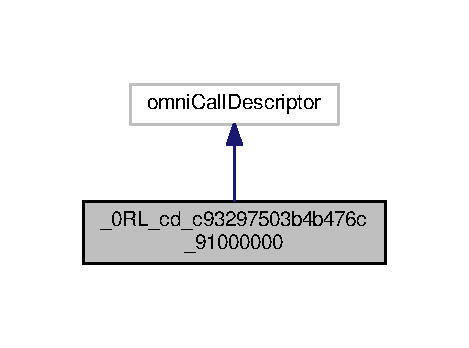
\includegraphics[width=225pt]{class__0_r_l__cd__c93297503b4b476c__91000000__inherit__graph}
\end{center}
\end{figure}


Collaboration diagram for \+\_\+0\+R\+L\+\_\+cd\+\_\+c93297503b4b476c\+\_\+91000000\+:
\nopagebreak
\begin{figure}[H]
\begin{center}
\leavevmode
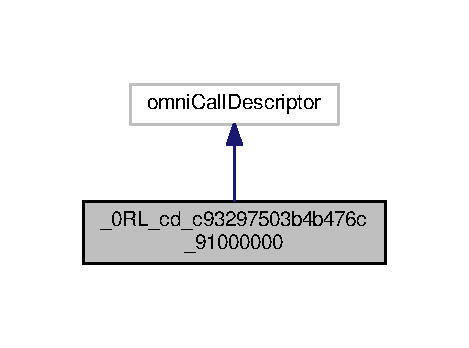
\includegraphics[width=225pt]{class__0_r_l__cd__c93297503b4b476c__91000000__coll__graph}
\end{center}
\end{figure}
\subsection*{Public Member Functions}
\begin{DoxyCompactItemize}
\item 
\hyperlink{class__0_r_l__cd__c93297503b4b476c__91000000_a0e586cea7a8d8ceb0da962954cefd98a}{\+\_\+0\+R\+L\+\_\+cd\+\_\+c93297503b4b476c\+\_\+91000000} (Local\+Call\+Fn lcfn, const char $\ast$op\+\_\+, size\+\_\+t oplen, \+\_\+\+C\+O\+R\+B\+A\+\_\+\+Boolean upcall=0)
\item 
void \hyperlink{class__0_r_l__cd__c93297503b4b476c__91000000_aeb147953bf0294500d507dff3bef0bf2}{marshal\+Arguments} (cdr\+Stream \&)
\item 
void \hyperlink{class__0_r_l__cd__c93297503b4b476c__91000000_a49bf2f2e30667c7fcfa189c0568abaa6}{unmarshal\+Arguments} (cdr\+Stream \&)
\end{DoxyCompactItemize}
\subsection*{Public Attributes}
\begin{DoxyCompactItemize}
\item 
\+::C\+O\+R\+B\+A\+::\+Double \hyperlink{class__0_r_l__cd__c93297503b4b476c__91000000_a87b6d297a7f1a56579d8d3fb6c3070f9}{arg\+\_\+0}
\item 
\+::C\+O\+R\+B\+A\+::\+Long \hyperlink{class__0_r_l__cd__c93297503b4b476c__91000000_a48914b58e05510223789862d5cbd7ec3}{arg\+\_\+1}
\end{DoxyCompactItemize}
\subsection*{Static Public Attributes}
\begin{DoxyCompactItemize}
\item 
static const char $\ast$const \hyperlink{class__0_r_l__cd__c93297503b4b476c__91000000_aa63022c9794a1db3032cf14c0946369e}{\+\_\+user\+\_\+exns} \mbox{[}$\,$\mbox{]}
\end{DoxyCompactItemize}


\subsection{Constructor \& Destructor Documentation}
\index{\+\_\+0\+R\+L\+\_\+cd\+\_\+c93297503b4b476c\+\_\+91000000@{\+\_\+0\+R\+L\+\_\+cd\+\_\+c93297503b4b476c\+\_\+91000000}!\+\_\+0\+R\+L\+\_\+cd\+\_\+c93297503b4b476c\+\_\+91000000@{\+\_\+0\+R\+L\+\_\+cd\+\_\+c93297503b4b476c\+\_\+91000000}}
\index{\+\_\+0\+R\+L\+\_\+cd\+\_\+c93297503b4b476c\+\_\+91000000@{\+\_\+0\+R\+L\+\_\+cd\+\_\+c93297503b4b476c\+\_\+91000000}!\+\_\+0\+R\+L\+\_\+cd\+\_\+c93297503b4b476c\+\_\+91000000@{\+\_\+0\+R\+L\+\_\+cd\+\_\+c93297503b4b476c\+\_\+91000000}}
\subsubsection[{\texorpdfstring{\+\_\+0\+R\+L\+\_\+cd\+\_\+c93297503b4b476c\+\_\+91000000(\+Local\+Call\+Fn lcfn, const char $\ast$op\+\_\+, size\+\_\+t oplen, \+\_\+\+C\+O\+R\+B\+A\+\_\+\+Boolean upcall=0)}{_0RL_cd_c93297503b4b476c_91000000(LocalCallFn lcfn, const char *op_, size_t oplen, _CORBA_Boolean upcall=0)}}]{\setlength{\rightskip}{0pt plus 5cm}\+\_\+0\+R\+L\+\_\+cd\+\_\+c93297503b4b476c\+\_\+91000000\+::\+\_\+0\+R\+L\+\_\+cd\+\_\+c93297503b4b476c\+\_\+91000000 (
\begin{DoxyParamCaption}
\item[{Local\+Call\+Fn}]{lcfn, }
\item[{const char $\ast$}]{op\+\_\+, }
\item[{size\+\_\+t}]{oplen, }
\item[{\+\_\+\+C\+O\+R\+B\+A\+\_\+\+Boolean}]{upcall = {\ttfamily 0}}
\end{DoxyParamCaption}
)\hspace{0.3cm}{\ttfamily [inline]}}\hypertarget{class__0_r_l__cd__c93297503b4b476c__91000000_a0e586cea7a8d8ceb0da962954cefd98a}{}\label{class__0_r_l__cd__c93297503b4b476c__91000000_a0e586cea7a8d8ceb0da962954cefd98a}


\subsection{Member Function Documentation}
\index{\+\_\+0\+R\+L\+\_\+cd\+\_\+c93297503b4b476c\+\_\+91000000@{\+\_\+0\+R\+L\+\_\+cd\+\_\+c93297503b4b476c\+\_\+91000000}!marshal\+Arguments@{marshal\+Arguments}}
\index{marshal\+Arguments@{marshal\+Arguments}!\+\_\+0\+R\+L\+\_\+cd\+\_\+c93297503b4b476c\+\_\+91000000@{\+\_\+0\+R\+L\+\_\+cd\+\_\+c93297503b4b476c\+\_\+91000000}}
\subsubsection[{\texorpdfstring{marshal\+Arguments(cdr\+Stream \&)}{marshalArguments(cdrStream &)}}]{\setlength{\rightskip}{0pt plus 5cm}void \+\_\+0\+R\+L\+\_\+cd\+\_\+c93297503b4b476c\+\_\+91000000\+::marshal\+Arguments (
\begin{DoxyParamCaption}
\item[{cdr\+Stream \&}]{\+\_\+n}
\end{DoxyParamCaption}
)}\hypertarget{class__0_r_l__cd__c93297503b4b476c__91000000_aeb147953bf0294500d507dff3bef0bf2}{}\label{class__0_r_l__cd__c93297503b4b476c__91000000_aeb147953bf0294500d507dff3bef0bf2}
\index{\+\_\+0\+R\+L\+\_\+cd\+\_\+c93297503b4b476c\+\_\+91000000@{\+\_\+0\+R\+L\+\_\+cd\+\_\+c93297503b4b476c\+\_\+91000000}!unmarshal\+Arguments@{unmarshal\+Arguments}}
\index{unmarshal\+Arguments@{unmarshal\+Arguments}!\+\_\+0\+R\+L\+\_\+cd\+\_\+c93297503b4b476c\+\_\+91000000@{\+\_\+0\+R\+L\+\_\+cd\+\_\+c93297503b4b476c\+\_\+91000000}}
\subsubsection[{\texorpdfstring{unmarshal\+Arguments(cdr\+Stream \&)}{unmarshalArguments(cdrStream &)}}]{\setlength{\rightskip}{0pt plus 5cm}void \+\_\+0\+R\+L\+\_\+cd\+\_\+c93297503b4b476c\+\_\+91000000\+::unmarshal\+Arguments (
\begin{DoxyParamCaption}
\item[{cdr\+Stream \&}]{\+\_\+n}
\end{DoxyParamCaption}
)}\hypertarget{class__0_r_l__cd__c93297503b4b476c__91000000_a49bf2f2e30667c7fcfa189c0568abaa6}{}\label{class__0_r_l__cd__c93297503b4b476c__91000000_a49bf2f2e30667c7fcfa189c0568abaa6}


\subsection{Member Data Documentation}
\index{\+\_\+0\+R\+L\+\_\+cd\+\_\+c93297503b4b476c\+\_\+91000000@{\+\_\+0\+R\+L\+\_\+cd\+\_\+c93297503b4b476c\+\_\+91000000}!\+\_\+user\+\_\+exns@{\+\_\+user\+\_\+exns}}
\index{\+\_\+user\+\_\+exns@{\+\_\+user\+\_\+exns}!\+\_\+0\+R\+L\+\_\+cd\+\_\+c93297503b4b476c\+\_\+91000000@{\+\_\+0\+R\+L\+\_\+cd\+\_\+c93297503b4b476c\+\_\+91000000}}
\subsubsection[{\texorpdfstring{\+\_\+user\+\_\+exns}{_user_exns}}]{\setlength{\rightskip}{0pt plus 5cm}const char $\ast$const \+\_\+0\+R\+L\+\_\+cd\+\_\+c93297503b4b476c\+\_\+91000000\+::\+\_\+user\+\_\+exns\hspace{0.3cm}{\ttfamily [static]}}\hypertarget{class__0_r_l__cd__c93297503b4b476c__91000000_aa63022c9794a1db3032cf14c0946369e}{}\label{class__0_r_l__cd__c93297503b4b476c__91000000_aa63022c9794a1db3032cf14c0946369e}
{\bfseries Initial value\+:}
\begin{DoxyCode}
= \{
  0
\}
\end{DoxyCode}
\index{\+\_\+0\+R\+L\+\_\+cd\+\_\+c93297503b4b476c\+\_\+91000000@{\+\_\+0\+R\+L\+\_\+cd\+\_\+c93297503b4b476c\+\_\+91000000}!arg\+\_\+0@{arg\+\_\+0}}
\index{arg\+\_\+0@{arg\+\_\+0}!\+\_\+0\+R\+L\+\_\+cd\+\_\+c93297503b4b476c\+\_\+91000000@{\+\_\+0\+R\+L\+\_\+cd\+\_\+c93297503b4b476c\+\_\+91000000}}
\subsubsection[{\texorpdfstring{arg\+\_\+0}{arg_0}}]{\setlength{\rightskip}{0pt plus 5cm}\+::C\+O\+R\+B\+A\+::\+Double \+\_\+0\+R\+L\+\_\+cd\+\_\+c93297503b4b476c\+\_\+91000000\+::arg\+\_\+0}\hypertarget{class__0_r_l__cd__c93297503b4b476c__91000000_a87b6d297a7f1a56579d8d3fb6c3070f9}{}\label{class__0_r_l__cd__c93297503b4b476c__91000000_a87b6d297a7f1a56579d8d3fb6c3070f9}
\index{\+\_\+0\+R\+L\+\_\+cd\+\_\+c93297503b4b476c\+\_\+91000000@{\+\_\+0\+R\+L\+\_\+cd\+\_\+c93297503b4b476c\+\_\+91000000}!arg\+\_\+1@{arg\+\_\+1}}
\index{arg\+\_\+1@{arg\+\_\+1}!\+\_\+0\+R\+L\+\_\+cd\+\_\+c93297503b4b476c\+\_\+91000000@{\+\_\+0\+R\+L\+\_\+cd\+\_\+c93297503b4b476c\+\_\+91000000}}
\subsubsection[{\texorpdfstring{arg\+\_\+1}{arg_1}}]{\setlength{\rightskip}{0pt plus 5cm}\+::C\+O\+R\+B\+A\+::\+Long \+\_\+0\+R\+L\+\_\+cd\+\_\+c93297503b4b476c\+\_\+91000000\+::arg\+\_\+1}\hypertarget{class__0_r_l__cd__c93297503b4b476c__91000000_a48914b58e05510223789862d5cbd7ec3}{}\label{class__0_r_l__cd__c93297503b4b476c__91000000_a48914b58e05510223789862d5cbd7ec3}


The documentation for this class was generated from the following file\+:\begin{DoxyCompactItemize}
\item 
src/\hyperlink{_petit_prince___stub_8cpp}{Petit\+Prince\+\_\+\+Stub.\+cpp}\end{DoxyCompactItemize}

\hypertarget{class__0_r_l__cd__c93297503b4b476c__b0000000}{}\section{\+\_\+0\+R\+L\+\_\+cd\+\_\+c93297503b4b476c\+\_\+b0000000 Class Reference}
\label{class__0_r_l__cd__c93297503b4b476c__b0000000}\index{\+\_\+0\+R\+L\+\_\+cd\+\_\+c93297503b4b476c\+\_\+b0000000@{\+\_\+0\+R\+L\+\_\+cd\+\_\+c93297503b4b476c\+\_\+b0000000}}


Inheritance diagram for \+\_\+0\+R\+L\+\_\+cd\+\_\+c93297503b4b476c\+\_\+b0000000\+:
\nopagebreak
\begin{figure}[H]
\begin{center}
\leavevmode
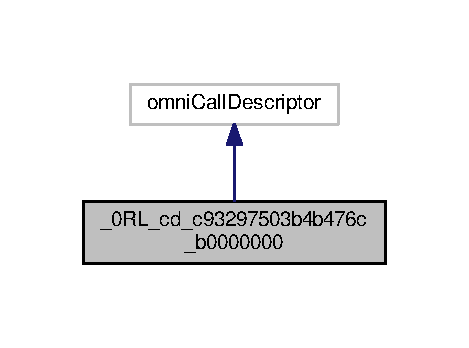
\includegraphics[width=225pt]{class__0_r_l__cd__c93297503b4b476c__b0000000__inherit__graph}
\end{center}
\end{figure}


Collaboration diagram for \+\_\+0\+R\+L\+\_\+cd\+\_\+c93297503b4b476c\+\_\+b0000000\+:
\nopagebreak
\begin{figure}[H]
\begin{center}
\leavevmode
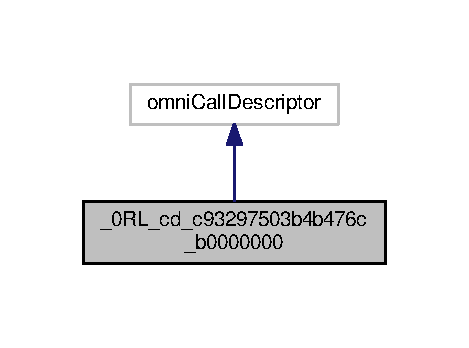
\includegraphics[width=225pt]{class__0_r_l__cd__c93297503b4b476c__b0000000__coll__graph}
\end{center}
\end{figure}
\subsection*{Public Member Functions}
\begin{DoxyCompactItemize}
\item 
\hyperlink{class__0_r_l__cd__c93297503b4b476c__b0000000_ac1cdd4fa506f30d39864cc6494deffc7}{\+\_\+0\+R\+L\+\_\+cd\+\_\+c93297503b4b476c\+\_\+b0000000} (Local\+Call\+Fn lcfn, const char $\ast$op\+\_\+, size\+\_\+t oplen, \+\_\+\+C\+O\+R\+B\+A\+\_\+\+Boolean upcall=0)
\item 
void \hyperlink{class__0_r_l__cd__c93297503b4b476c__b0000000_a5226a30e633968374c01cfb591480fde}{marshal\+Arguments} (cdr\+Stream \&)
\item 
void \hyperlink{class__0_r_l__cd__c93297503b4b476c__b0000000_a190389d98b14853f4e10da3b7c7dbce6}{unmarshal\+Arguments} (cdr\+Stream \&)
\item 
void \hyperlink{class__0_r_l__cd__c93297503b4b476c__b0000000_a0f138774eeeb7ecad8f9d98186941e2c}{user\+Exception} (cdr\+Stream \&, \+\_\+\+O\+M\+N\+I\+\_\+\+NS(I\+O\+P\+\_\+C)$\ast$, const char $\ast$)
\end{DoxyCompactItemize}
\subsection*{Public Attributes}
\begin{DoxyCompactItemize}
\item 
\+::C\+O\+R\+B\+A\+::\+Long \hyperlink{class__0_r_l__cd__c93297503b4b476c__b0000000_ae90df0f02cbdd0ef4f1add610ebd2118}{arg\+\_\+0}
\item 
\+::C\+O\+R\+B\+A\+::\+Long \hyperlink{class__0_r_l__cd__c93297503b4b476c__b0000000_a02271bbb9282eb05747774e2e14e7ffb}{arg\+\_\+1}
\end{DoxyCompactItemize}
\subsection*{Static Public Attributes}
\begin{DoxyCompactItemize}
\item 
static const char $\ast$const \hyperlink{class__0_r_l__cd__c93297503b4b476c__b0000000_a03a219aaf4b2d7bcc60274a72583f9d8}{\+\_\+user\+\_\+exns} \mbox{[}$\,$\mbox{]}
\end{DoxyCompactItemize}


\subsection{Constructor \& Destructor Documentation}
\index{\+\_\+0\+R\+L\+\_\+cd\+\_\+c93297503b4b476c\+\_\+b0000000@{\+\_\+0\+R\+L\+\_\+cd\+\_\+c93297503b4b476c\+\_\+b0000000}!\+\_\+0\+R\+L\+\_\+cd\+\_\+c93297503b4b476c\+\_\+b0000000@{\+\_\+0\+R\+L\+\_\+cd\+\_\+c93297503b4b476c\+\_\+b0000000}}
\index{\+\_\+0\+R\+L\+\_\+cd\+\_\+c93297503b4b476c\+\_\+b0000000@{\+\_\+0\+R\+L\+\_\+cd\+\_\+c93297503b4b476c\+\_\+b0000000}!\+\_\+0\+R\+L\+\_\+cd\+\_\+c93297503b4b476c\+\_\+b0000000@{\+\_\+0\+R\+L\+\_\+cd\+\_\+c93297503b4b476c\+\_\+b0000000}}
\subsubsection[{\texorpdfstring{\+\_\+0\+R\+L\+\_\+cd\+\_\+c93297503b4b476c\+\_\+b0000000(\+Local\+Call\+Fn lcfn, const char $\ast$op\+\_\+, size\+\_\+t oplen, \+\_\+\+C\+O\+R\+B\+A\+\_\+\+Boolean upcall=0)}{_0RL_cd_c93297503b4b476c_b0000000(LocalCallFn lcfn, const char *op_, size_t oplen, _CORBA_Boolean upcall=0)}}]{\setlength{\rightskip}{0pt plus 5cm}\+\_\+0\+R\+L\+\_\+cd\+\_\+c93297503b4b476c\+\_\+b0000000\+::\+\_\+0\+R\+L\+\_\+cd\+\_\+c93297503b4b476c\+\_\+b0000000 (
\begin{DoxyParamCaption}
\item[{Local\+Call\+Fn}]{lcfn, }
\item[{const char $\ast$}]{op\+\_\+, }
\item[{size\+\_\+t}]{oplen, }
\item[{\+\_\+\+C\+O\+R\+B\+A\+\_\+\+Boolean}]{upcall = {\ttfamily 0}}
\end{DoxyParamCaption}
)\hspace{0.3cm}{\ttfamily [inline]}}\hypertarget{class__0_r_l__cd__c93297503b4b476c__b0000000_ac1cdd4fa506f30d39864cc6494deffc7}{}\label{class__0_r_l__cd__c93297503b4b476c__b0000000_ac1cdd4fa506f30d39864cc6494deffc7}


\subsection{Member Function Documentation}
\index{\+\_\+0\+R\+L\+\_\+cd\+\_\+c93297503b4b476c\+\_\+b0000000@{\+\_\+0\+R\+L\+\_\+cd\+\_\+c93297503b4b476c\+\_\+b0000000}!marshal\+Arguments@{marshal\+Arguments}}
\index{marshal\+Arguments@{marshal\+Arguments}!\+\_\+0\+R\+L\+\_\+cd\+\_\+c93297503b4b476c\+\_\+b0000000@{\+\_\+0\+R\+L\+\_\+cd\+\_\+c93297503b4b476c\+\_\+b0000000}}
\subsubsection[{\texorpdfstring{marshal\+Arguments(cdr\+Stream \&)}{marshalArguments(cdrStream &)}}]{\setlength{\rightskip}{0pt plus 5cm}void \+\_\+0\+R\+L\+\_\+cd\+\_\+c93297503b4b476c\+\_\+b0000000\+::marshal\+Arguments (
\begin{DoxyParamCaption}
\item[{cdr\+Stream \&}]{\+\_\+n}
\end{DoxyParamCaption}
)}\hypertarget{class__0_r_l__cd__c93297503b4b476c__b0000000_a5226a30e633968374c01cfb591480fde}{}\label{class__0_r_l__cd__c93297503b4b476c__b0000000_a5226a30e633968374c01cfb591480fde}
\index{\+\_\+0\+R\+L\+\_\+cd\+\_\+c93297503b4b476c\+\_\+b0000000@{\+\_\+0\+R\+L\+\_\+cd\+\_\+c93297503b4b476c\+\_\+b0000000}!unmarshal\+Arguments@{unmarshal\+Arguments}}
\index{unmarshal\+Arguments@{unmarshal\+Arguments}!\+\_\+0\+R\+L\+\_\+cd\+\_\+c93297503b4b476c\+\_\+b0000000@{\+\_\+0\+R\+L\+\_\+cd\+\_\+c93297503b4b476c\+\_\+b0000000}}
\subsubsection[{\texorpdfstring{unmarshal\+Arguments(cdr\+Stream \&)}{unmarshalArguments(cdrStream &)}}]{\setlength{\rightskip}{0pt plus 5cm}void \+\_\+0\+R\+L\+\_\+cd\+\_\+c93297503b4b476c\+\_\+b0000000\+::unmarshal\+Arguments (
\begin{DoxyParamCaption}
\item[{cdr\+Stream \&}]{\+\_\+n}
\end{DoxyParamCaption}
)}\hypertarget{class__0_r_l__cd__c93297503b4b476c__b0000000_a190389d98b14853f4e10da3b7c7dbce6}{}\label{class__0_r_l__cd__c93297503b4b476c__b0000000_a190389d98b14853f4e10da3b7c7dbce6}
\index{\+\_\+0\+R\+L\+\_\+cd\+\_\+c93297503b4b476c\+\_\+b0000000@{\+\_\+0\+R\+L\+\_\+cd\+\_\+c93297503b4b476c\+\_\+b0000000}!user\+Exception@{user\+Exception}}
\index{user\+Exception@{user\+Exception}!\+\_\+0\+R\+L\+\_\+cd\+\_\+c93297503b4b476c\+\_\+b0000000@{\+\_\+0\+R\+L\+\_\+cd\+\_\+c93297503b4b476c\+\_\+b0000000}}
\subsubsection[{\texorpdfstring{user\+Exception(cdr\+Stream \&, \+\_\+\+O\+M\+N\+I\+\_\+\+N\+S(\+I\+O\+P\+\_\+\+C)$\ast$, const char $\ast$)}{userException(cdrStream &, _OMNI_NS(IOP_C)*, const char *)}}]{\setlength{\rightskip}{0pt plus 5cm}void \+\_\+0\+R\+L\+\_\+cd\+\_\+c93297503b4b476c\+\_\+b0000000\+::user\+Exception (
\begin{DoxyParamCaption}
\item[{cdr\+Stream \&}]{s, }
\item[{\+\_\+\+O\+M\+N\+I\+\_\+\+NS(I\+O\+P\+\_\+C)$\ast$}]{iop\+\_\+client, }
\item[{const char $\ast$}]{repo\+Id}
\end{DoxyParamCaption}
)}\hypertarget{class__0_r_l__cd__c93297503b4b476c__b0000000_a0f138774eeeb7ecad8f9d98186941e2c}{}\label{class__0_r_l__cd__c93297503b4b476c__b0000000_a0f138774eeeb7ecad8f9d98186941e2c}


\subsection{Member Data Documentation}
\index{\+\_\+0\+R\+L\+\_\+cd\+\_\+c93297503b4b476c\+\_\+b0000000@{\+\_\+0\+R\+L\+\_\+cd\+\_\+c93297503b4b476c\+\_\+b0000000}!\+\_\+user\+\_\+exns@{\+\_\+user\+\_\+exns}}
\index{\+\_\+user\+\_\+exns@{\+\_\+user\+\_\+exns}!\+\_\+0\+R\+L\+\_\+cd\+\_\+c93297503b4b476c\+\_\+b0000000@{\+\_\+0\+R\+L\+\_\+cd\+\_\+c93297503b4b476c\+\_\+b0000000}}
\subsubsection[{\texorpdfstring{\+\_\+user\+\_\+exns}{_user_exns}}]{\setlength{\rightskip}{0pt plus 5cm}const char $\ast$const \+\_\+0\+R\+L\+\_\+cd\+\_\+c93297503b4b476c\+\_\+b0000000\+::\+\_\+user\+\_\+exns\hspace{0.3cm}{\ttfamily [static]}}\hypertarget{class__0_r_l__cd__c93297503b4b476c__b0000000_a03a219aaf4b2d7bcc60274a72583f9d8}{}\label{class__0_r_l__cd__c93297503b4b476c__b0000000_a03a219aaf4b2d7bcc60274a72583f9d8}
{\bfseries Initial value\+:}
\begin{DoxyCode}
= \{
  PetitPrince::DrawService::UnexpectedDraw::\_PD\_repoId
\}
\end{DoxyCode}
\index{\+\_\+0\+R\+L\+\_\+cd\+\_\+c93297503b4b476c\+\_\+b0000000@{\+\_\+0\+R\+L\+\_\+cd\+\_\+c93297503b4b476c\+\_\+b0000000}!arg\+\_\+0@{arg\+\_\+0}}
\index{arg\+\_\+0@{arg\+\_\+0}!\+\_\+0\+R\+L\+\_\+cd\+\_\+c93297503b4b476c\+\_\+b0000000@{\+\_\+0\+R\+L\+\_\+cd\+\_\+c93297503b4b476c\+\_\+b0000000}}
\subsubsection[{\texorpdfstring{arg\+\_\+0}{arg_0}}]{\setlength{\rightskip}{0pt plus 5cm}\+::C\+O\+R\+B\+A\+::\+Long \+\_\+0\+R\+L\+\_\+cd\+\_\+c93297503b4b476c\+\_\+b0000000\+::arg\+\_\+0}\hypertarget{class__0_r_l__cd__c93297503b4b476c__b0000000_ae90df0f02cbdd0ef4f1add610ebd2118}{}\label{class__0_r_l__cd__c93297503b4b476c__b0000000_ae90df0f02cbdd0ef4f1add610ebd2118}
\index{\+\_\+0\+R\+L\+\_\+cd\+\_\+c93297503b4b476c\+\_\+b0000000@{\+\_\+0\+R\+L\+\_\+cd\+\_\+c93297503b4b476c\+\_\+b0000000}!arg\+\_\+1@{arg\+\_\+1}}
\index{arg\+\_\+1@{arg\+\_\+1}!\+\_\+0\+R\+L\+\_\+cd\+\_\+c93297503b4b476c\+\_\+b0000000@{\+\_\+0\+R\+L\+\_\+cd\+\_\+c93297503b4b476c\+\_\+b0000000}}
\subsubsection[{\texorpdfstring{arg\+\_\+1}{arg_1}}]{\setlength{\rightskip}{0pt plus 5cm}\+::C\+O\+R\+B\+A\+::\+Long \+\_\+0\+R\+L\+\_\+cd\+\_\+c93297503b4b476c\+\_\+b0000000\+::arg\+\_\+1}\hypertarget{class__0_r_l__cd__c93297503b4b476c__b0000000_a02271bbb9282eb05747774e2e14e7ffb}{}\label{class__0_r_l__cd__c93297503b4b476c__b0000000_a02271bbb9282eb05747774e2e14e7ffb}


The documentation for this class was generated from the following file\+:\begin{DoxyCompactItemize}
\item 
src/\hyperlink{_petit_prince___stub_8cpp}{Petit\+Prince\+\_\+\+Stub.\+cpp}\end{DoxyCompactItemize}

\hypertarget{class__0_r_l__cd__c93297503b4b476c__d0000000}{}\section{\+\_\+0\+R\+L\+\_\+cd\+\_\+c93297503b4b476c\+\_\+d0000000 Class Reference}
\label{class__0_r_l__cd__c93297503b4b476c__d0000000}\index{\+\_\+0\+R\+L\+\_\+cd\+\_\+c93297503b4b476c\+\_\+d0000000@{\+\_\+0\+R\+L\+\_\+cd\+\_\+c93297503b4b476c\+\_\+d0000000}}


Inheritance diagram for \+\_\+0\+R\+L\+\_\+cd\+\_\+c93297503b4b476c\+\_\+d0000000\+:
\nopagebreak
\begin{figure}[H]
\begin{center}
\leavevmode
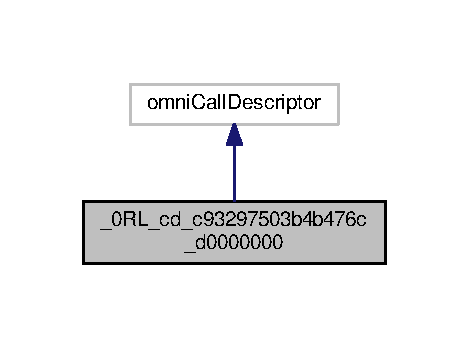
\includegraphics[width=225pt]{class__0_r_l__cd__c93297503b4b476c__d0000000__inherit__graph}
\end{center}
\end{figure}


Collaboration diagram for \+\_\+0\+R\+L\+\_\+cd\+\_\+c93297503b4b476c\+\_\+d0000000\+:
\nopagebreak
\begin{figure}[H]
\begin{center}
\leavevmode
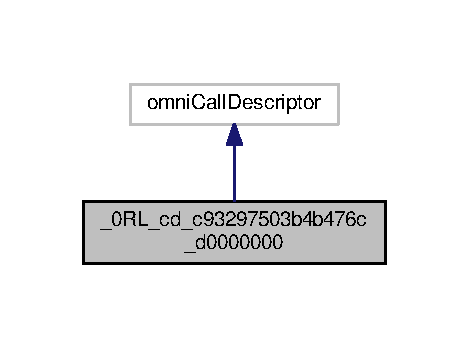
\includegraphics[width=225pt]{class__0_r_l__cd__c93297503b4b476c__d0000000__coll__graph}
\end{center}
\end{figure}
\subsection*{Public Member Functions}
\begin{DoxyCompactItemize}
\item 
\hyperlink{class__0_r_l__cd__c93297503b4b476c__d0000000_adfa0c552b20d7a74a4ac468399094266}{\+\_\+0\+R\+L\+\_\+cd\+\_\+c93297503b4b476c\+\_\+d0000000} (Local\+Call\+Fn lcfn, const char $\ast$op\+\_\+, size\+\_\+t oplen, \+\_\+\+C\+O\+R\+B\+A\+\_\+\+Boolean upcall=0)
\item 
void \hyperlink{class__0_r_l__cd__c93297503b4b476c__d0000000_a9ab3a00a9409f5b3c7a39f7202822419}{marshal\+Arguments} (cdr\+Stream \&)
\item 
void \hyperlink{class__0_r_l__cd__c93297503b4b476c__d0000000_ab9dfcf580415a9e3f925e724fd5afe1a}{unmarshal\+Arguments} (cdr\+Stream \&)
\item 
void \hyperlink{class__0_r_l__cd__c93297503b4b476c__d0000000_a4d49e0707d79223d0b13517125ed9cc1}{unmarshal\+Returned\+Values} (cdr\+Stream \&)
\item 
void \hyperlink{class__0_r_l__cd__c93297503b4b476c__d0000000_a276cc2d40feb9cd8ea0aa2956b164d6f}{marshal\+Returned\+Values} (cdr\+Stream \&)
\end{DoxyCompactItemize}
\subsection*{Public Attributes}
\begin{DoxyCompactItemize}
\item 
\+::C\+O\+R\+B\+A\+::\+Long \hyperlink{class__0_r_l__cd__c93297503b4b476c__d0000000_a3f9faa5564ca3e53589bb5523fdf15f2}{arg\+\_\+0}
\item 
\+::C\+O\+R\+B\+A\+::\+String\+\_\+var \hyperlink{class__0_r_l__cd__c93297503b4b476c__d0000000_a85333e8615ac624f1ed70841d68adc3a}{result}
\end{DoxyCompactItemize}
\subsection*{Static Public Attributes}
\begin{DoxyCompactItemize}
\item 
static const char $\ast$const \hyperlink{class__0_r_l__cd__c93297503b4b476c__d0000000_aa32c9fe871a1a705e7e880c5220be36c}{\+\_\+user\+\_\+exns} \mbox{[}$\,$\mbox{]}
\end{DoxyCompactItemize}


\subsection{Detailed Description}


Definition at line 1519 of file Petit\+Prince\+\_\+\+Stub.\+cpp.



\subsection{Constructor \& Destructor Documentation}
\index{\+\_\+0\+R\+L\+\_\+cd\+\_\+c93297503b4b476c\+\_\+d0000000@{\+\_\+0\+R\+L\+\_\+cd\+\_\+c93297503b4b476c\+\_\+d0000000}!\+\_\+0\+R\+L\+\_\+cd\+\_\+c93297503b4b476c\+\_\+d0000000@{\+\_\+0\+R\+L\+\_\+cd\+\_\+c93297503b4b476c\+\_\+d0000000}}
\index{\+\_\+0\+R\+L\+\_\+cd\+\_\+c93297503b4b476c\+\_\+d0000000@{\+\_\+0\+R\+L\+\_\+cd\+\_\+c93297503b4b476c\+\_\+d0000000}!\+\_\+0\+R\+L\+\_\+cd\+\_\+c93297503b4b476c\+\_\+d0000000@{\+\_\+0\+R\+L\+\_\+cd\+\_\+c93297503b4b476c\+\_\+d0000000}}
\subsubsection[{\texorpdfstring{\+\_\+0\+R\+L\+\_\+cd\+\_\+c93297503b4b476c\+\_\+d0000000(\+Local\+Call\+Fn lcfn, const char $\ast$op\+\_\+, size\+\_\+t oplen, \+\_\+\+C\+O\+R\+B\+A\+\_\+\+Boolean upcall=0)}{_0RL_cd_c93297503b4b476c_d0000000(LocalCallFn lcfn, const char *op_, size_t oplen, _CORBA_Boolean upcall=0)}}]{\setlength{\rightskip}{0pt plus 5cm}\+\_\+0\+R\+L\+\_\+cd\+\_\+c93297503b4b476c\+\_\+d0000000\+::\+\_\+0\+R\+L\+\_\+cd\+\_\+c93297503b4b476c\+\_\+d0000000 (
\begin{DoxyParamCaption}
\item[{Local\+Call\+Fn}]{lcfn, }
\item[{const char $\ast$}]{op\+\_\+, }
\item[{size\+\_\+t}]{oplen, }
\item[{\+\_\+\+C\+O\+R\+B\+A\+\_\+\+Boolean}]{upcall = {\ttfamily 0}}
\end{DoxyParamCaption}
)\hspace{0.3cm}{\ttfamily [inline]}}\hypertarget{class__0_r_l__cd__c93297503b4b476c__d0000000_adfa0c552b20d7a74a4ac468399094266}{}\label{class__0_r_l__cd__c93297503b4b476c__d0000000_adfa0c552b20d7a74a4ac468399094266}


Definition at line 1523 of file Petit\+Prince\+\_\+\+Stub.\+cpp.



\subsection{Member Function Documentation}
\index{\+\_\+0\+R\+L\+\_\+cd\+\_\+c93297503b4b476c\+\_\+d0000000@{\+\_\+0\+R\+L\+\_\+cd\+\_\+c93297503b4b476c\+\_\+d0000000}!marshal\+Arguments@{marshal\+Arguments}}
\index{marshal\+Arguments@{marshal\+Arguments}!\+\_\+0\+R\+L\+\_\+cd\+\_\+c93297503b4b476c\+\_\+d0000000@{\+\_\+0\+R\+L\+\_\+cd\+\_\+c93297503b4b476c\+\_\+d0000000}}
\subsubsection[{\texorpdfstring{marshal\+Arguments(cdr\+Stream \&)}{marshalArguments(cdrStream &)}}]{\setlength{\rightskip}{0pt plus 5cm}void \+\_\+0\+R\+L\+\_\+cd\+\_\+c93297503b4b476c\+\_\+d0000000\+::marshal\+Arguments (
\begin{DoxyParamCaption}
\item[{cdr\+Stream \&}]{\+\_\+n}
\end{DoxyParamCaption}
)}\hypertarget{class__0_r_l__cd__c93297503b4b476c__d0000000_a9ab3a00a9409f5b3c7a39f7202822419}{}\label{class__0_r_l__cd__c93297503b4b476c__d0000000_a9ab3a00a9409f5b3c7a39f7202822419}


Definition at line 1542 of file Petit\+Prince\+\_\+\+Stub.\+cpp.

\index{\+\_\+0\+R\+L\+\_\+cd\+\_\+c93297503b4b476c\+\_\+d0000000@{\+\_\+0\+R\+L\+\_\+cd\+\_\+c93297503b4b476c\+\_\+d0000000}!marshal\+Returned\+Values@{marshal\+Returned\+Values}}
\index{marshal\+Returned\+Values@{marshal\+Returned\+Values}!\+\_\+0\+R\+L\+\_\+cd\+\_\+c93297503b4b476c\+\_\+d0000000@{\+\_\+0\+R\+L\+\_\+cd\+\_\+c93297503b4b476c\+\_\+d0000000}}
\subsubsection[{\texorpdfstring{marshal\+Returned\+Values(cdr\+Stream \&)}{marshalReturnedValues(cdrStream &)}}]{\setlength{\rightskip}{0pt plus 5cm}void \+\_\+0\+R\+L\+\_\+cd\+\_\+c93297503b4b476c\+\_\+d0000000\+::marshal\+Returned\+Values (
\begin{DoxyParamCaption}
\item[{cdr\+Stream \&}]{\+\_\+n}
\end{DoxyParamCaption}
)}\hypertarget{class__0_r_l__cd__c93297503b4b476c__d0000000_a276cc2d40feb9cd8ea0aa2956b164d6f}{}\label{class__0_r_l__cd__c93297503b4b476c__d0000000_a276cc2d40feb9cd8ea0aa2956b164d6f}


Definition at line 1554 of file Petit\+Prince\+\_\+\+Stub.\+cpp.

\index{\+\_\+0\+R\+L\+\_\+cd\+\_\+c93297503b4b476c\+\_\+d0000000@{\+\_\+0\+R\+L\+\_\+cd\+\_\+c93297503b4b476c\+\_\+d0000000}!unmarshal\+Arguments@{unmarshal\+Arguments}}
\index{unmarshal\+Arguments@{unmarshal\+Arguments}!\+\_\+0\+R\+L\+\_\+cd\+\_\+c93297503b4b476c\+\_\+d0000000@{\+\_\+0\+R\+L\+\_\+cd\+\_\+c93297503b4b476c\+\_\+d0000000}}
\subsubsection[{\texorpdfstring{unmarshal\+Arguments(cdr\+Stream \&)}{unmarshalArguments(cdrStream &)}}]{\setlength{\rightskip}{0pt plus 5cm}void \+\_\+0\+R\+L\+\_\+cd\+\_\+c93297503b4b476c\+\_\+d0000000\+::unmarshal\+Arguments (
\begin{DoxyParamCaption}
\item[{cdr\+Stream \&}]{\+\_\+n}
\end{DoxyParamCaption}
)}\hypertarget{class__0_r_l__cd__c93297503b4b476c__d0000000_ab9dfcf580415a9e3f925e724fd5afe1a}{}\label{class__0_r_l__cd__c93297503b4b476c__d0000000_ab9dfcf580415a9e3f925e724fd5afe1a}


Definition at line 1548 of file Petit\+Prince\+\_\+\+Stub.\+cpp.

\index{\+\_\+0\+R\+L\+\_\+cd\+\_\+c93297503b4b476c\+\_\+d0000000@{\+\_\+0\+R\+L\+\_\+cd\+\_\+c93297503b4b476c\+\_\+d0000000}!unmarshal\+Returned\+Values@{unmarshal\+Returned\+Values}}
\index{unmarshal\+Returned\+Values@{unmarshal\+Returned\+Values}!\+\_\+0\+R\+L\+\_\+cd\+\_\+c93297503b4b476c\+\_\+d0000000@{\+\_\+0\+R\+L\+\_\+cd\+\_\+c93297503b4b476c\+\_\+d0000000}}
\subsubsection[{\texorpdfstring{unmarshal\+Returned\+Values(cdr\+Stream \&)}{unmarshalReturnedValues(cdrStream &)}}]{\setlength{\rightskip}{0pt plus 5cm}void \+\_\+0\+R\+L\+\_\+cd\+\_\+c93297503b4b476c\+\_\+d0000000\+::unmarshal\+Returned\+Values (
\begin{DoxyParamCaption}
\item[{cdr\+Stream \&}]{\+\_\+n}
\end{DoxyParamCaption}
)}\hypertarget{class__0_r_l__cd__c93297503b4b476c__d0000000_a4d49e0707d79223d0b13517125ed9cc1}{}\label{class__0_r_l__cd__c93297503b4b476c__d0000000_a4d49e0707d79223d0b13517125ed9cc1}


Definition at line 1560 of file Petit\+Prince\+\_\+\+Stub.\+cpp.



\subsection{Member Data Documentation}
\index{\+\_\+0\+R\+L\+\_\+cd\+\_\+c93297503b4b476c\+\_\+d0000000@{\+\_\+0\+R\+L\+\_\+cd\+\_\+c93297503b4b476c\+\_\+d0000000}!\+\_\+user\+\_\+exns@{\+\_\+user\+\_\+exns}}
\index{\+\_\+user\+\_\+exns@{\+\_\+user\+\_\+exns}!\+\_\+0\+R\+L\+\_\+cd\+\_\+c93297503b4b476c\+\_\+d0000000@{\+\_\+0\+R\+L\+\_\+cd\+\_\+c93297503b4b476c\+\_\+d0000000}}
\subsubsection[{\texorpdfstring{\+\_\+user\+\_\+exns}{_user_exns}}]{\setlength{\rightskip}{0pt plus 5cm}const char $\ast$const \+\_\+0\+R\+L\+\_\+cd\+\_\+c93297503b4b476c\+\_\+d0000000\+::\+\_\+user\+\_\+exns\hspace{0.3cm}{\ttfamily [static]}}\hypertarget{class__0_r_l__cd__c93297503b4b476c__d0000000_aa32c9fe871a1a705e7e880c5220be36c}{}\label{class__0_r_l__cd__c93297503b4b476c__d0000000_aa32c9fe871a1a705e7e880c5220be36c}
{\bfseries Initial value\+:}
\begin{DoxyCode}
= \{
  0
\}
\end{DoxyCode}


Definition at line 1536 of file Petit\+Prince\+\_\+\+Stub.\+cpp.

\index{\+\_\+0\+R\+L\+\_\+cd\+\_\+c93297503b4b476c\+\_\+d0000000@{\+\_\+0\+R\+L\+\_\+cd\+\_\+c93297503b4b476c\+\_\+d0000000}!arg\+\_\+0@{arg\+\_\+0}}
\index{arg\+\_\+0@{arg\+\_\+0}!\+\_\+0\+R\+L\+\_\+cd\+\_\+c93297503b4b476c\+\_\+d0000000@{\+\_\+0\+R\+L\+\_\+cd\+\_\+c93297503b4b476c\+\_\+d0000000}}
\subsubsection[{\texorpdfstring{arg\+\_\+0}{arg_0}}]{\setlength{\rightskip}{0pt plus 5cm}\+::C\+O\+R\+B\+A\+::\+Long \+\_\+0\+R\+L\+\_\+cd\+\_\+c93297503b4b476c\+\_\+d0000000\+::arg\+\_\+0}\hypertarget{class__0_r_l__cd__c93297503b4b476c__d0000000_a3f9faa5564ca3e53589bb5523fdf15f2}{}\label{class__0_r_l__cd__c93297503b4b476c__d0000000_a3f9faa5564ca3e53589bb5523fdf15f2}


Definition at line 1538 of file Petit\+Prince\+\_\+\+Stub.\+cpp.

\index{\+\_\+0\+R\+L\+\_\+cd\+\_\+c93297503b4b476c\+\_\+d0000000@{\+\_\+0\+R\+L\+\_\+cd\+\_\+c93297503b4b476c\+\_\+d0000000}!result@{result}}
\index{result@{result}!\+\_\+0\+R\+L\+\_\+cd\+\_\+c93297503b4b476c\+\_\+d0000000@{\+\_\+0\+R\+L\+\_\+cd\+\_\+c93297503b4b476c\+\_\+d0000000}}
\subsubsection[{\texorpdfstring{result}{result}}]{\setlength{\rightskip}{0pt plus 5cm}\+::C\+O\+R\+B\+A\+::\+String\+\_\+var \+\_\+0\+R\+L\+\_\+cd\+\_\+c93297503b4b476c\+\_\+d0000000\+::result}\hypertarget{class__0_r_l__cd__c93297503b4b476c__d0000000_a85333e8615ac624f1ed70841d68adc3a}{}\label{class__0_r_l__cd__c93297503b4b476c__d0000000_a85333e8615ac624f1ed70841d68adc3a}


Definition at line 1539 of file Petit\+Prince\+\_\+\+Stub.\+cpp.



The documentation for this class was generated from the following file\+:\begin{DoxyCompactItemize}
\item 
src/\hyperlink{_petit_prince___stub_8cpp}{Petit\+Prince\+\_\+\+Stub.\+cpp}\end{DoxyCompactItemize}

\hypertarget{class__0_r_l__cd__c93297503b4b476c__f0000000}{}\section{\+\_\+0\+R\+L\+\_\+cd\+\_\+c93297503b4b476c\+\_\+f0000000 Class Reference}
\label{class__0_r_l__cd__c93297503b4b476c__f0000000}\index{\+\_\+0\+R\+L\+\_\+cd\+\_\+c93297503b4b476c\+\_\+f0000000@{\+\_\+0\+R\+L\+\_\+cd\+\_\+c93297503b4b476c\+\_\+f0000000}}


Inheritance diagram for \+\_\+0\+R\+L\+\_\+cd\+\_\+c93297503b4b476c\+\_\+f0000000\+:
\nopagebreak
\begin{figure}[H]
\begin{center}
\leavevmode
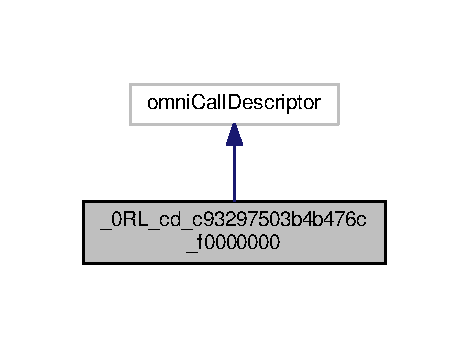
\includegraphics[width=225pt]{class__0_r_l__cd__c93297503b4b476c__f0000000__inherit__graph}
\end{center}
\end{figure}


Collaboration diagram for \+\_\+0\+R\+L\+\_\+cd\+\_\+c93297503b4b476c\+\_\+f0000000\+:
\nopagebreak
\begin{figure}[H]
\begin{center}
\leavevmode
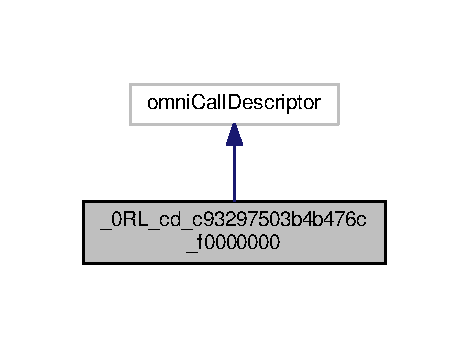
\includegraphics[width=225pt]{class__0_r_l__cd__c93297503b4b476c__f0000000__coll__graph}
\end{center}
\end{figure}
\subsection*{Public Member Functions}
\begin{DoxyCompactItemize}
\item 
\hyperlink{class__0_r_l__cd__c93297503b4b476c__f0000000_ad3eaa0ebc00da7dc742dbdbf31095bad}{\+\_\+0\+R\+L\+\_\+cd\+\_\+c93297503b4b476c\+\_\+f0000000} (Local\+Call\+Fn lcfn, const char $\ast$op\+\_\+, size\+\_\+t oplen, \+\_\+\+C\+O\+R\+B\+A\+\_\+\+Boolean upcall=0)
\item 
void \hyperlink{class__0_r_l__cd__c93297503b4b476c__f0000000_a81f267829bab9ba9088cc742c8ef5af6}{marshal\+Arguments} (cdr\+Stream \&)
\item 
void \hyperlink{class__0_r_l__cd__c93297503b4b476c__f0000000_aceadb2c1efea07e6ea96340a919763b0}{unmarshal\+Arguments} (cdr\+Stream \&)
\item 
void \hyperlink{class__0_r_l__cd__c93297503b4b476c__f0000000_ad7fbed03bef53a7c91eae50bc47d595d}{unmarshal\+Returned\+Values} (cdr\+Stream \&)
\item 
void \hyperlink{class__0_r_l__cd__c93297503b4b476c__f0000000_add6ae989d8ee5c498af741e94cee1008}{marshal\+Returned\+Values} (cdr\+Stream \&)
\item 
void \hyperlink{class__0_r_l__cd__c93297503b4b476c__f0000000_a1deb1933f6e9069a955129ac562a283f}{user\+Exception} (cdr\+Stream \&, \+\_\+\+O\+M\+N\+I\+\_\+\+NS(I\+O\+P\+\_\+C)$\ast$, const char $\ast$)
\end{DoxyCompactItemize}
\subsection*{Public Attributes}
\begin{DoxyCompactItemize}
\item 
\+::C\+O\+R\+B\+A\+::\+String\+\_\+var \hyperlink{class__0_r_l__cd__c93297503b4b476c__f0000000_a42f779a55d1f4fd887c74846dd62c7ee}{arg\+\_\+0\+\_\+}
\item 
const char $\ast$ \hyperlink{class__0_r_l__cd__c93297503b4b476c__f0000000_acfd83eca6ef903b69b6c90c5b2f5bba3}{arg\+\_\+0}
\item 
Petit\+Prince\+::\+Point \hyperlink{class__0_r_l__cd__c93297503b4b476c__f0000000_aba17f6503cd4d839e8e4da44faa81214}{arg\+\_\+1\+\_\+}
\item 
const Petit\+Prince\+::\+Point $\ast$ \hyperlink{class__0_r_l__cd__c93297503b4b476c__f0000000_a5eaa35de47a96874f0d9a7ad3b791900}{arg\+\_\+1}
\item 
Petit\+Prince\+::\+Point \hyperlink{class__0_r_l__cd__c93297503b4b476c__f0000000_ac6451cd86d3d5189dc4125fec3ba3906}{arg\+\_\+2\+\_\+}
\item 
const Petit\+Prince\+::\+Point $\ast$ \hyperlink{class__0_r_l__cd__c93297503b4b476c__f0000000_aa1250982102c136edb168de08a43b793}{arg\+\_\+2}
\item 
\+::C\+O\+R\+B\+A\+::\+Long \hyperlink{class__0_r_l__cd__c93297503b4b476c__f0000000_a2a668d01c3ab8f7a926dd60b837aa99d}{result}
\end{DoxyCompactItemize}
\subsection*{Static Public Attributes}
\begin{DoxyCompactItemize}
\item 
static const char $\ast$const \hyperlink{class__0_r_l__cd__c93297503b4b476c__f0000000_aea4851e36117b25ae65ca009c10f2b79}{\+\_\+user\+\_\+exns} \mbox{[}$\,$\mbox{]}
\end{DoxyCompactItemize}


\subsection{Detailed Description}


Definition at line 1897 of file Petit\+Prince\+\_\+\+Stub.\+cpp.



\subsection{Constructor \& Destructor Documentation}
\index{\+\_\+0\+R\+L\+\_\+cd\+\_\+c93297503b4b476c\+\_\+f0000000@{\+\_\+0\+R\+L\+\_\+cd\+\_\+c93297503b4b476c\+\_\+f0000000}!\+\_\+0\+R\+L\+\_\+cd\+\_\+c93297503b4b476c\+\_\+f0000000@{\+\_\+0\+R\+L\+\_\+cd\+\_\+c93297503b4b476c\+\_\+f0000000}}
\index{\+\_\+0\+R\+L\+\_\+cd\+\_\+c93297503b4b476c\+\_\+f0000000@{\+\_\+0\+R\+L\+\_\+cd\+\_\+c93297503b4b476c\+\_\+f0000000}!\+\_\+0\+R\+L\+\_\+cd\+\_\+c93297503b4b476c\+\_\+f0000000@{\+\_\+0\+R\+L\+\_\+cd\+\_\+c93297503b4b476c\+\_\+f0000000}}
\subsubsection[{\texorpdfstring{\+\_\+0\+R\+L\+\_\+cd\+\_\+c93297503b4b476c\+\_\+f0000000(\+Local\+Call\+Fn lcfn, const char $\ast$op\+\_\+, size\+\_\+t oplen, \+\_\+\+C\+O\+R\+B\+A\+\_\+\+Boolean upcall=0)}{_0RL_cd_c93297503b4b476c_f0000000(LocalCallFn lcfn, const char *op_, size_t oplen, _CORBA_Boolean upcall=0)}}]{\setlength{\rightskip}{0pt plus 5cm}\+\_\+0\+R\+L\+\_\+cd\+\_\+c93297503b4b476c\+\_\+f0000000\+::\+\_\+0\+R\+L\+\_\+cd\+\_\+c93297503b4b476c\+\_\+f0000000 (
\begin{DoxyParamCaption}
\item[{Local\+Call\+Fn}]{lcfn, }
\item[{const char $\ast$}]{op\+\_\+, }
\item[{size\+\_\+t}]{oplen, }
\item[{\+\_\+\+C\+O\+R\+B\+A\+\_\+\+Boolean}]{upcall = {\ttfamily 0}}
\end{DoxyParamCaption}
)\hspace{0.3cm}{\ttfamily [inline]}}\hypertarget{class__0_r_l__cd__c93297503b4b476c__f0000000_ad3eaa0ebc00da7dc742dbdbf31095bad}{}\label{class__0_r_l__cd__c93297503b4b476c__f0000000_ad3eaa0ebc00da7dc742dbdbf31095bad}


Definition at line 1901 of file Petit\+Prince\+\_\+\+Stub.\+cpp.



\subsection{Member Function Documentation}
\index{\+\_\+0\+R\+L\+\_\+cd\+\_\+c93297503b4b476c\+\_\+f0000000@{\+\_\+0\+R\+L\+\_\+cd\+\_\+c93297503b4b476c\+\_\+f0000000}!marshal\+Arguments@{marshal\+Arguments}}
\index{marshal\+Arguments@{marshal\+Arguments}!\+\_\+0\+R\+L\+\_\+cd\+\_\+c93297503b4b476c\+\_\+f0000000@{\+\_\+0\+R\+L\+\_\+cd\+\_\+c93297503b4b476c\+\_\+f0000000}}
\subsubsection[{\texorpdfstring{marshal\+Arguments(cdr\+Stream \&)}{marshalArguments(cdrStream &)}}]{\setlength{\rightskip}{0pt plus 5cm}void \+\_\+0\+R\+L\+\_\+cd\+\_\+c93297503b4b476c\+\_\+f0000000\+::marshal\+Arguments (
\begin{DoxyParamCaption}
\item[{cdr\+Stream \&}]{\+\_\+n}
\end{DoxyParamCaption}
)}\hypertarget{class__0_r_l__cd__c93297503b4b476c__f0000000_a81f267829bab9ba9088cc742c8ef5af6}{}\label{class__0_r_l__cd__c93297503b4b476c__f0000000_a81f267829bab9ba9088cc742c8ef5af6}


Definition at line 1925 of file Petit\+Prince\+\_\+\+Stub.\+cpp.

\index{\+\_\+0\+R\+L\+\_\+cd\+\_\+c93297503b4b476c\+\_\+f0000000@{\+\_\+0\+R\+L\+\_\+cd\+\_\+c93297503b4b476c\+\_\+f0000000}!marshal\+Returned\+Values@{marshal\+Returned\+Values}}
\index{marshal\+Returned\+Values@{marshal\+Returned\+Values}!\+\_\+0\+R\+L\+\_\+cd\+\_\+c93297503b4b476c\+\_\+f0000000@{\+\_\+0\+R\+L\+\_\+cd\+\_\+c93297503b4b476c\+\_\+f0000000}}
\subsubsection[{\texorpdfstring{marshal\+Returned\+Values(cdr\+Stream \&)}{marshalReturnedValues(cdrStream &)}}]{\setlength{\rightskip}{0pt plus 5cm}void \+\_\+0\+R\+L\+\_\+cd\+\_\+c93297503b4b476c\+\_\+f0000000\+::marshal\+Returned\+Values (
\begin{DoxyParamCaption}
\item[{cdr\+Stream \&}]{\+\_\+n}
\end{DoxyParamCaption}
)}\hypertarget{class__0_r_l__cd__c93297503b4b476c__f0000000_add6ae989d8ee5c498af741e94cee1008}{}\label{class__0_r_l__cd__c93297503b4b476c__f0000000_add6ae989d8ee5c498af741e94cee1008}


Definition at line 1944 of file Petit\+Prince\+\_\+\+Stub.\+cpp.

\index{\+\_\+0\+R\+L\+\_\+cd\+\_\+c93297503b4b476c\+\_\+f0000000@{\+\_\+0\+R\+L\+\_\+cd\+\_\+c93297503b4b476c\+\_\+f0000000}!unmarshal\+Arguments@{unmarshal\+Arguments}}
\index{unmarshal\+Arguments@{unmarshal\+Arguments}!\+\_\+0\+R\+L\+\_\+cd\+\_\+c93297503b4b476c\+\_\+f0000000@{\+\_\+0\+R\+L\+\_\+cd\+\_\+c93297503b4b476c\+\_\+f0000000}}
\subsubsection[{\texorpdfstring{unmarshal\+Arguments(cdr\+Stream \&)}{unmarshalArguments(cdrStream &)}}]{\setlength{\rightskip}{0pt plus 5cm}void \+\_\+0\+R\+L\+\_\+cd\+\_\+c93297503b4b476c\+\_\+f0000000\+::unmarshal\+Arguments (
\begin{DoxyParamCaption}
\item[{cdr\+Stream \&}]{\+\_\+n}
\end{DoxyParamCaption}
)}\hypertarget{class__0_r_l__cd__c93297503b4b476c__f0000000_aceadb2c1efea07e6ea96340a919763b0}{}\label{class__0_r_l__cd__c93297503b4b476c__f0000000_aceadb2c1efea07e6ea96340a919763b0}


Definition at line 1933 of file Petit\+Prince\+\_\+\+Stub.\+cpp.

\index{\+\_\+0\+R\+L\+\_\+cd\+\_\+c93297503b4b476c\+\_\+f0000000@{\+\_\+0\+R\+L\+\_\+cd\+\_\+c93297503b4b476c\+\_\+f0000000}!unmarshal\+Returned\+Values@{unmarshal\+Returned\+Values}}
\index{unmarshal\+Returned\+Values@{unmarshal\+Returned\+Values}!\+\_\+0\+R\+L\+\_\+cd\+\_\+c93297503b4b476c\+\_\+f0000000@{\+\_\+0\+R\+L\+\_\+cd\+\_\+c93297503b4b476c\+\_\+f0000000}}
\subsubsection[{\texorpdfstring{unmarshal\+Returned\+Values(cdr\+Stream \&)}{unmarshalReturnedValues(cdrStream &)}}]{\setlength{\rightskip}{0pt plus 5cm}void \+\_\+0\+R\+L\+\_\+cd\+\_\+c93297503b4b476c\+\_\+f0000000\+::unmarshal\+Returned\+Values (
\begin{DoxyParamCaption}
\item[{cdr\+Stream \&}]{\+\_\+n}
\end{DoxyParamCaption}
)}\hypertarget{class__0_r_l__cd__c93297503b4b476c__f0000000_ad7fbed03bef53a7c91eae50bc47d595d}{}\label{class__0_r_l__cd__c93297503b4b476c__f0000000_ad7fbed03bef53a7c91eae50bc47d595d}


Definition at line 1950 of file Petit\+Prince\+\_\+\+Stub.\+cpp.

\index{\+\_\+0\+R\+L\+\_\+cd\+\_\+c93297503b4b476c\+\_\+f0000000@{\+\_\+0\+R\+L\+\_\+cd\+\_\+c93297503b4b476c\+\_\+f0000000}!user\+Exception@{user\+Exception}}
\index{user\+Exception@{user\+Exception}!\+\_\+0\+R\+L\+\_\+cd\+\_\+c93297503b4b476c\+\_\+f0000000@{\+\_\+0\+R\+L\+\_\+cd\+\_\+c93297503b4b476c\+\_\+f0000000}}
\subsubsection[{\texorpdfstring{user\+Exception(cdr\+Stream \&, \+\_\+\+O\+M\+N\+I\+\_\+\+N\+S(\+I\+O\+P\+\_\+\+C)$\ast$, const char $\ast$)}{userException(cdrStream &, _OMNI_NS(IOP_C)*, const char *)}}]{\setlength{\rightskip}{0pt plus 5cm}void \+\_\+0\+R\+L\+\_\+cd\+\_\+c93297503b4b476c\+\_\+f0000000\+::user\+Exception (
\begin{DoxyParamCaption}
\item[{cdr\+Stream \&}]{s, }
\item[{\+\_\+\+O\+M\+N\+I\+\_\+\+NS(I\+O\+P\+\_\+C)$\ast$}]{iop\+\_\+client, }
\item[{const char $\ast$}]{repo\+Id}
\end{DoxyParamCaption}
)}\hypertarget{class__0_r_l__cd__c93297503b4b476c__f0000000_a1deb1933f6e9069a955129ac562a283f}{}\label{class__0_r_l__cd__c93297503b4b476c__f0000000_a1deb1933f6e9069a955129ac562a283f}


Definition at line 1960 of file Petit\+Prince\+\_\+\+Stub.\+cpp.



\subsection{Member Data Documentation}
\index{\+\_\+0\+R\+L\+\_\+cd\+\_\+c93297503b4b476c\+\_\+f0000000@{\+\_\+0\+R\+L\+\_\+cd\+\_\+c93297503b4b476c\+\_\+f0000000}!\+\_\+user\+\_\+exns@{\+\_\+user\+\_\+exns}}
\index{\+\_\+user\+\_\+exns@{\+\_\+user\+\_\+exns}!\+\_\+0\+R\+L\+\_\+cd\+\_\+c93297503b4b476c\+\_\+f0000000@{\+\_\+0\+R\+L\+\_\+cd\+\_\+c93297503b4b476c\+\_\+f0000000}}
\subsubsection[{\texorpdfstring{\+\_\+user\+\_\+exns}{_user_exns}}]{\setlength{\rightskip}{0pt plus 5cm}const char $\ast$const \+\_\+0\+R\+L\+\_\+cd\+\_\+c93297503b4b476c\+\_\+f0000000\+::\+\_\+user\+\_\+exns\hspace{0.3cm}{\ttfamily [static]}}\hypertarget{class__0_r_l__cd__c93297503b4b476c__f0000000_aea4851e36117b25ae65ca009c10f2b79}{}\label{class__0_r_l__cd__c93297503b4b476c__f0000000_aea4851e36117b25ae65ca009c10f2b79}
{\bfseries Initial value\+:}
\begin{DoxyCode}
= \{
  PetitPrince::PetitPrinceService::InvalidDrawParams::\_PD\_repoId
\}
\end{DoxyCode}


Definition at line 1914 of file Petit\+Prince\+\_\+\+Stub.\+cpp.

\index{\+\_\+0\+R\+L\+\_\+cd\+\_\+c93297503b4b476c\+\_\+f0000000@{\+\_\+0\+R\+L\+\_\+cd\+\_\+c93297503b4b476c\+\_\+f0000000}!arg\+\_\+0@{arg\+\_\+0}}
\index{arg\+\_\+0@{arg\+\_\+0}!\+\_\+0\+R\+L\+\_\+cd\+\_\+c93297503b4b476c\+\_\+f0000000@{\+\_\+0\+R\+L\+\_\+cd\+\_\+c93297503b4b476c\+\_\+f0000000}}
\subsubsection[{\texorpdfstring{arg\+\_\+0}{arg_0}}]{\setlength{\rightskip}{0pt plus 5cm}const char$\ast$ \+\_\+0\+R\+L\+\_\+cd\+\_\+c93297503b4b476c\+\_\+f0000000\+::arg\+\_\+0}\hypertarget{class__0_r_l__cd__c93297503b4b476c__f0000000_acfd83eca6ef903b69b6c90c5b2f5bba3}{}\label{class__0_r_l__cd__c93297503b4b476c__f0000000_acfd83eca6ef903b69b6c90c5b2f5bba3}


Definition at line 1917 of file Petit\+Prince\+\_\+\+Stub.\+cpp.

\index{\+\_\+0\+R\+L\+\_\+cd\+\_\+c93297503b4b476c\+\_\+f0000000@{\+\_\+0\+R\+L\+\_\+cd\+\_\+c93297503b4b476c\+\_\+f0000000}!arg\+\_\+0\+\_\+@{arg\+\_\+0\+\_\+}}
\index{arg\+\_\+0\+\_\+@{arg\+\_\+0\+\_\+}!\+\_\+0\+R\+L\+\_\+cd\+\_\+c93297503b4b476c\+\_\+f0000000@{\+\_\+0\+R\+L\+\_\+cd\+\_\+c93297503b4b476c\+\_\+f0000000}}
\subsubsection[{\texorpdfstring{arg\+\_\+0\+\_\+}{arg_0_}}]{\setlength{\rightskip}{0pt plus 5cm}\+::C\+O\+R\+B\+A\+::\+String\+\_\+var \+\_\+0\+R\+L\+\_\+cd\+\_\+c93297503b4b476c\+\_\+f0000000\+::arg\+\_\+0\+\_\+}\hypertarget{class__0_r_l__cd__c93297503b4b476c__f0000000_a42f779a55d1f4fd887c74846dd62c7ee}{}\label{class__0_r_l__cd__c93297503b4b476c__f0000000_a42f779a55d1f4fd887c74846dd62c7ee}


Definition at line 1916 of file Petit\+Prince\+\_\+\+Stub.\+cpp.

\index{\+\_\+0\+R\+L\+\_\+cd\+\_\+c93297503b4b476c\+\_\+f0000000@{\+\_\+0\+R\+L\+\_\+cd\+\_\+c93297503b4b476c\+\_\+f0000000}!arg\+\_\+1@{arg\+\_\+1}}
\index{arg\+\_\+1@{arg\+\_\+1}!\+\_\+0\+R\+L\+\_\+cd\+\_\+c93297503b4b476c\+\_\+f0000000@{\+\_\+0\+R\+L\+\_\+cd\+\_\+c93297503b4b476c\+\_\+f0000000}}
\subsubsection[{\texorpdfstring{arg\+\_\+1}{arg_1}}]{\setlength{\rightskip}{0pt plus 5cm}const Petit\+Prince\+::\+Point$\ast$ \+\_\+0\+R\+L\+\_\+cd\+\_\+c93297503b4b476c\+\_\+f0000000\+::arg\+\_\+1}\hypertarget{class__0_r_l__cd__c93297503b4b476c__f0000000_a5eaa35de47a96874f0d9a7ad3b791900}{}\label{class__0_r_l__cd__c93297503b4b476c__f0000000_a5eaa35de47a96874f0d9a7ad3b791900}


Definition at line 1919 of file Petit\+Prince\+\_\+\+Stub.\+cpp.

\index{\+\_\+0\+R\+L\+\_\+cd\+\_\+c93297503b4b476c\+\_\+f0000000@{\+\_\+0\+R\+L\+\_\+cd\+\_\+c93297503b4b476c\+\_\+f0000000}!arg\+\_\+1\+\_\+@{arg\+\_\+1\+\_\+}}
\index{arg\+\_\+1\+\_\+@{arg\+\_\+1\+\_\+}!\+\_\+0\+R\+L\+\_\+cd\+\_\+c93297503b4b476c\+\_\+f0000000@{\+\_\+0\+R\+L\+\_\+cd\+\_\+c93297503b4b476c\+\_\+f0000000}}
\subsubsection[{\texorpdfstring{arg\+\_\+1\+\_\+}{arg_1_}}]{\setlength{\rightskip}{0pt plus 5cm}Petit\+Prince\+::\+Point \+\_\+0\+R\+L\+\_\+cd\+\_\+c93297503b4b476c\+\_\+f0000000\+::arg\+\_\+1\+\_\+}\hypertarget{class__0_r_l__cd__c93297503b4b476c__f0000000_aba17f6503cd4d839e8e4da44faa81214}{}\label{class__0_r_l__cd__c93297503b4b476c__f0000000_aba17f6503cd4d839e8e4da44faa81214}


Definition at line 1918 of file Petit\+Prince\+\_\+\+Stub.\+cpp.

\index{\+\_\+0\+R\+L\+\_\+cd\+\_\+c93297503b4b476c\+\_\+f0000000@{\+\_\+0\+R\+L\+\_\+cd\+\_\+c93297503b4b476c\+\_\+f0000000}!arg\+\_\+2@{arg\+\_\+2}}
\index{arg\+\_\+2@{arg\+\_\+2}!\+\_\+0\+R\+L\+\_\+cd\+\_\+c93297503b4b476c\+\_\+f0000000@{\+\_\+0\+R\+L\+\_\+cd\+\_\+c93297503b4b476c\+\_\+f0000000}}
\subsubsection[{\texorpdfstring{arg\+\_\+2}{arg_2}}]{\setlength{\rightskip}{0pt plus 5cm}const Petit\+Prince\+::\+Point$\ast$ \+\_\+0\+R\+L\+\_\+cd\+\_\+c93297503b4b476c\+\_\+f0000000\+::arg\+\_\+2}\hypertarget{class__0_r_l__cd__c93297503b4b476c__f0000000_aa1250982102c136edb168de08a43b793}{}\label{class__0_r_l__cd__c93297503b4b476c__f0000000_aa1250982102c136edb168de08a43b793}


Definition at line 1921 of file Petit\+Prince\+\_\+\+Stub.\+cpp.

\index{\+\_\+0\+R\+L\+\_\+cd\+\_\+c93297503b4b476c\+\_\+f0000000@{\+\_\+0\+R\+L\+\_\+cd\+\_\+c93297503b4b476c\+\_\+f0000000}!arg\+\_\+2\+\_\+@{arg\+\_\+2\+\_\+}}
\index{arg\+\_\+2\+\_\+@{arg\+\_\+2\+\_\+}!\+\_\+0\+R\+L\+\_\+cd\+\_\+c93297503b4b476c\+\_\+f0000000@{\+\_\+0\+R\+L\+\_\+cd\+\_\+c93297503b4b476c\+\_\+f0000000}}
\subsubsection[{\texorpdfstring{arg\+\_\+2\+\_\+}{arg_2_}}]{\setlength{\rightskip}{0pt plus 5cm}Petit\+Prince\+::\+Point \+\_\+0\+R\+L\+\_\+cd\+\_\+c93297503b4b476c\+\_\+f0000000\+::arg\+\_\+2\+\_\+}\hypertarget{class__0_r_l__cd__c93297503b4b476c__f0000000_ac6451cd86d3d5189dc4125fec3ba3906}{}\label{class__0_r_l__cd__c93297503b4b476c__f0000000_ac6451cd86d3d5189dc4125fec3ba3906}


Definition at line 1920 of file Petit\+Prince\+\_\+\+Stub.\+cpp.

\index{\+\_\+0\+R\+L\+\_\+cd\+\_\+c93297503b4b476c\+\_\+f0000000@{\+\_\+0\+R\+L\+\_\+cd\+\_\+c93297503b4b476c\+\_\+f0000000}!result@{result}}
\index{result@{result}!\+\_\+0\+R\+L\+\_\+cd\+\_\+c93297503b4b476c\+\_\+f0000000@{\+\_\+0\+R\+L\+\_\+cd\+\_\+c93297503b4b476c\+\_\+f0000000}}
\subsubsection[{\texorpdfstring{result}{result}}]{\setlength{\rightskip}{0pt plus 5cm}\+::C\+O\+R\+B\+A\+::\+Long \+\_\+0\+R\+L\+\_\+cd\+\_\+c93297503b4b476c\+\_\+f0000000\+::result}\hypertarget{class__0_r_l__cd__c93297503b4b476c__f0000000_a2a668d01c3ab8f7a926dd60b837aa99d}{}\label{class__0_r_l__cd__c93297503b4b476c__f0000000_a2a668d01c3ab8f7a926dd60b837aa99d}


Definition at line 1922 of file Petit\+Prince\+\_\+\+Stub.\+cpp.



The documentation for this class was generated from the following file\+:\begin{DoxyCompactItemize}
\item 
src/\hyperlink{_petit_prince___stub_8cpp}{Petit\+Prince\+\_\+\+Stub.\+cpp}\end{DoxyCompactItemize}

\hypertarget{class__0_r_l__insert_to_any___singleton____c_petit_prince__m_draw_service__m_non_applicable}{}\section{\+\_\+0\+R\+L\+\_\+insert\+To\+Any\+\_\+\+Singleton\+\_\+\+\_\+c\+Petit\+Prince\+\_\+m\+Draw\+Service\+\_\+m\+Non\+Applicable Class Reference}
\label{class__0_r_l__insert_to_any___singleton____c_petit_prince__m_draw_service__m_non_applicable}\index{\+\_\+0\+R\+L\+\_\+insert\+To\+Any\+\_\+\+Singleton\+\_\+\+\_\+c\+Petit\+Prince\+\_\+m\+Draw\+Service\+\_\+m\+Non\+Applicable@{\+\_\+0\+R\+L\+\_\+insert\+To\+Any\+\_\+\+Singleton\+\_\+\+\_\+c\+Petit\+Prince\+\_\+m\+Draw\+Service\+\_\+m\+Non\+Applicable}}
\subsection*{Public Member Functions}
\begin{DoxyCompactItemize}
\item 
\hyperlink{class__0_r_l__insert_to_any___singleton____c_petit_prince__m_draw_service__m_non_applicable_af3f2fae89265f27a44d183a06ba284f3}{\+\_\+0\+R\+L\+\_\+insert\+To\+Any\+\_\+\+Singleton\+\_\+\+\_\+c\+Petit\+Prince\+\_\+m\+Draw\+Service\+\_\+m\+Non\+Applicable} ()
\end{DoxyCompactItemize}


\subsection{Detailed Description}


Definition at line 720 of file Petit\+Prince\+\_\+\+Dyn\+Stub.\+cpp.



\subsection{Constructor \& Destructor Documentation}
\index{\+\_\+0\+R\+L\+\_\+insert\+To\+Any\+\_\+\+Singleton\+\_\+\+\_\+c\+Petit\+Prince\+\_\+m\+Draw\+Service\+\_\+m\+Non\+Applicable@{\+\_\+0\+R\+L\+\_\+insert\+To\+Any\+\_\+\+Singleton\+\_\+\+\_\+c\+Petit\+Prince\+\_\+m\+Draw\+Service\+\_\+m\+Non\+Applicable}!\+\_\+0\+R\+L\+\_\+insert\+To\+Any\+\_\+\+Singleton\+\_\+\+\_\+c\+Petit\+Prince\+\_\+m\+Draw\+Service\+\_\+m\+Non\+Applicable@{\+\_\+0\+R\+L\+\_\+insert\+To\+Any\+\_\+\+Singleton\+\_\+\+\_\+c\+Petit\+Prince\+\_\+m\+Draw\+Service\+\_\+m\+Non\+Applicable}}
\index{\+\_\+0\+R\+L\+\_\+insert\+To\+Any\+\_\+\+Singleton\+\_\+\+\_\+c\+Petit\+Prince\+\_\+m\+Draw\+Service\+\_\+m\+Non\+Applicable@{\+\_\+0\+R\+L\+\_\+insert\+To\+Any\+\_\+\+Singleton\+\_\+\+\_\+c\+Petit\+Prince\+\_\+m\+Draw\+Service\+\_\+m\+Non\+Applicable}!\+\_\+0\+R\+L\+\_\+insert\+To\+Any\+\_\+\+Singleton\+\_\+\+\_\+c\+Petit\+Prince\+\_\+m\+Draw\+Service\+\_\+m\+Non\+Applicable@{\+\_\+0\+R\+L\+\_\+insert\+To\+Any\+\_\+\+Singleton\+\_\+\+\_\+c\+Petit\+Prince\+\_\+m\+Draw\+Service\+\_\+m\+Non\+Applicable}}
\subsubsection[{\texorpdfstring{\+\_\+0\+R\+L\+\_\+insert\+To\+Any\+\_\+\+Singleton\+\_\+\+\_\+c\+Petit\+Prince\+\_\+m\+Draw\+Service\+\_\+m\+Non\+Applicable()}{_0RL_insertToAny_Singleton__cPetitPrince_mDrawService_mNonApplicable()}}]{\setlength{\rightskip}{0pt plus 5cm}\+\_\+0\+R\+L\+\_\+insert\+To\+Any\+\_\+\+Singleton\+\_\+\+\_\+c\+Petit\+Prince\+\_\+m\+Draw\+Service\+\_\+m\+Non\+Applicable\+::\+\_\+0\+R\+L\+\_\+insert\+To\+Any\+\_\+\+Singleton\+\_\+\+\_\+c\+Petit\+Prince\+\_\+m\+Draw\+Service\+\_\+m\+Non\+Applicable (
\begin{DoxyParamCaption}
{}
\end{DoxyParamCaption}
)\hspace{0.3cm}{\ttfamily [inline]}}\hypertarget{class__0_r_l__insert_to_any___singleton____c_petit_prince__m_draw_service__m_non_applicable_af3f2fae89265f27a44d183a06ba284f3}{}\label{class__0_r_l__insert_to_any___singleton____c_petit_prince__m_draw_service__m_non_applicable_af3f2fae89265f27a44d183a06ba284f3}


Definition at line 722 of file Petit\+Prince\+\_\+\+Dyn\+Stub.\+cpp.



The documentation for this class was generated from the following file\+:\begin{DoxyCompactItemize}
\item 
src/\hyperlink{_petit_prince___dyn_stub_8cpp}{Petit\+Prince\+\_\+\+Dyn\+Stub.\+cpp}\end{DoxyCompactItemize}

\hypertarget{class__0_r_l__insert_to_any___singleton____c_petit_prince__m_draw_service__m_unexpected_draw}{}\section{\+\_\+0\+R\+L\+\_\+insert\+To\+Any\+\_\+\+Singleton\+\_\+\+\_\+c\+Petit\+Prince\+\_\+m\+Draw\+Service\+\_\+m\+Unexpected\+Draw Class Reference}
\label{class__0_r_l__insert_to_any___singleton____c_petit_prince__m_draw_service__m_unexpected_draw}\index{\+\_\+0\+R\+L\+\_\+insert\+To\+Any\+\_\+\+Singleton\+\_\+\+\_\+c\+Petit\+Prince\+\_\+m\+Draw\+Service\+\_\+m\+Unexpected\+Draw@{\+\_\+0\+R\+L\+\_\+insert\+To\+Any\+\_\+\+Singleton\+\_\+\+\_\+c\+Petit\+Prince\+\_\+m\+Draw\+Service\+\_\+m\+Unexpected\+Draw}}
\subsection*{Public Member Functions}
\begin{DoxyCompactItemize}
\item 
\hyperlink{class__0_r_l__insert_to_any___singleton____c_petit_prince__m_draw_service__m_unexpected_draw_a2befe43881bf8af05235572cd732e9e2}{\+\_\+0\+R\+L\+\_\+insert\+To\+Any\+\_\+\+Singleton\+\_\+\+\_\+c\+Petit\+Prince\+\_\+m\+Draw\+Service\+\_\+m\+Unexpected\+Draw} ()
\end{DoxyCompactItemize}


\subsection{Detailed Description}


Definition at line 787 of file Petit\+Prince\+\_\+\+Dyn\+Stub.\+cpp.



\subsection{Constructor \& Destructor Documentation}
\index{\+\_\+0\+R\+L\+\_\+insert\+To\+Any\+\_\+\+Singleton\+\_\+\+\_\+c\+Petit\+Prince\+\_\+m\+Draw\+Service\+\_\+m\+Unexpected\+Draw@{\+\_\+0\+R\+L\+\_\+insert\+To\+Any\+\_\+\+Singleton\+\_\+\+\_\+c\+Petit\+Prince\+\_\+m\+Draw\+Service\+\_\+m\+Unexpected\+Draw}!\+\_\+0\+R\+L\+\_\+insert\+To\+Any\+\_\+\+Singleton\+\_\+\+\_\+c\+Petit\+Prince\+\_\+m\+Draw\+Service\+\_\+m\+Unexpected\+Draw@{\+\_\+0\+R\+L\+\_\+insert\+To\+Any\+\_\+\+Singleton\+\_\+\+\_\+c\+Petit\+Prince\+\_\+m\+Draw\+Service\+\_\+m\+Unexpected\+Draw}}
\index{\+\_\+0\+R\+L\+\_\+insert\+To\+Any\+\_\+\+Singleton\+\_\+\+\_\+c\+Petit\+Prince\+\_\+m\+Draw\+Service\+\_\+m\+Unexpected\+Draw@{\+\_\+0\+R\+L\+\_\+insert\+To\+Any\+\_\+\+Singleton\+\_\+\+\_\+c\+Petit\+Prince\+\_\+m\+Draw\+Service\+\_\+m\+Unexpected\+Draw}!\+\_\+0\+R\+L\+\_\+insert\+To\+Any\+\_\+\+Singleton\+\_\+\+\_\+c\+Petit\+Prince\+\_\+m\+Draw\+Service\+\_\+m\+Unexpected\+Draw@{\+\_\+0\+R\+L\+\_\+insert\+To\+Any\+\_\+\+Singleton\+\_\+\+\_\+c\+Petit\+Prince\+\_\+m\+Draw\+Service\+\_\+m\+Unexpected\+Draw}}
\subsubsection[{\texorpdfstring{\+\_\+0\+R\+L\+\_\+insert\+To\+Any\+\_\+\+Singleton\+\_\+\+\_\+c\+Petit\+Prince\+\_\+m\+Draw\+Service\+\_\+m\+Unexpected\+Draw()}{_0RL_insertToAny_Singleton__cPetitPrince_mDrawService_mUnexpectedDraw()}}]{\setlength{\rightskip}{0pt plus 5cm}\+\_\+0\+R\+L\+\_\+insert\+To\+Any\+\_\+\+Singleton\+\_\+\+\_\+c\+Petit\+Prince\+\_\+m\+Draw\+Service\+\_\+m\+Unexpected\+Draw\+::\+\_\+0\+R\+L\+\_\+insert\+To\+Any\+\_\+\+Singleton\+\_\+\+\_\+c\+Petit\+Prince\+\_\+m\+Draw\+Service\+\_\+m\+Unexpected\+Draw (
\begin{DoxyParamCaption}
{}
\end{DoxyParamCaption}
)\hspace{0.3cm}{\ttfamily [inline]}}\hypertarget{class__0_r_l__insert_to_any___singleton____c_petit_prince__m_draw_service__m_unexpected_draw_a2befe43881bf8af05235572cd732e9e2}{}\label{class__0_r_l__insert_to_any___singleton____c_petit_prince__m_draw_service__m_unexpected_draw_a2befe43881bf8af05235572cd732e9e2}


Definition at line 789 of file Petit\+Prince\+\_\+\+Dyn\+Stub.\+cpp.



The documentation for this class was generated from the following file\+:\begin{DoxyCompactItemize}
\item 
src/\hyperlink{_petit_prince___dyn_stub_8cpp}{Petit\+Prince\+\_\+\+Dyn\+Stub.\+cpp}\end{DoxyCompactItemize}

\hypertarget{class__0_r_l__insert_to_any___singleton____c_petit_prince__m_petit_prince_service__m_invalid_draw_params}{}\section{\+\_\+0\+R\+L\+\_\+insert\+To\+Any\+\_\+\+Singleton\+\_\+\+\_\+c\+Petit\+Prince\+\_\+m\+Petit\+Prince\+Service\+\_\+m\+Invalid\+Draw\+Params Class Reference}
\label{class__0_r_l__insert_to_any___singleton____c_petit_prince__m_petit_prince_service__m_invalid_draw_params}\index{\+\_\+0\+R\+L\+\_\+insert\+To\+Any\+\_\+\+Singleton\+\_\+\+\_\+c\+Petit\+Prince\+\_\+m\+Petit\+Prince\+Service\+\_\+m\+Invalid\+Draw\+Params@{\+\_\+0\+R\+L\+\_\+insert\+To\+Any\+\_\+\+Singleton\+\_\+\+\_\+c\+Petit\+Prince\+\_\+m\+Petit\+Prince\+Service\+\_\+m\+Invalid\+Draw\+Params}}
\subsection*{Public Member Functions}
\begin{DoxyCompactItemize}
\item 
\hyperlink{class__0_r_l__insert_to_any___singleton____c_petit_prince__m_petit_prince_service__m_invalid_draw_params_a2493851c25d8c242bff78f58c9a63e8e}{\+\_\+0\+R\+L\+\_\+insert\+To\+Any\+\_\+\+Singleton\+\_\+\+\_\+c\+Petit\+Prince\+\_\+m\+Petit\+Prince\+Service\+\_\+m\+Invalid\+Draw\+Params} ()
\end{DoxyCompactItemize}


\subsection{Detailed Description}


Definition at line 906 of file Petit\+Prince\+\_\+\+Dyn\+Stub.\+cpp.



\subsection{Constructor \& Destructor Documentation}
\index{\+\_\+0\+R\+L\+\_\+insert\+To\+Any\+\_\+\+Singleton\+\_\+\+\_\+c\+Petit\+Prince\+\_\+m\+Petit\+Prince\+Service\+\_\+m\+Invalid\+Draw\+Params@{\+\_\+0\+R\+L\+\_\+insert\+To\+Any\+\_\+\+Singleton\+\_\+\+\_\+c\+Petit\+Prince\+\_\+m\+Petit\+Prince\+Service\+\_\+m\+Invalid\+Draw\+Params}!\+\_\+0\+R\+L\+\_\+insert\+To\+Any\+\_\+\+Singleton\+\_\+\+\_\+c\+Petit\+Prince\+\_\+m\+Petit\+Prince\+Service\+\_\+m\+Invalid\+Draw\+Params@{\+\_\+0\+R\+L\+\_\+insert\+To\+Any\+\_\+\+Singleton\+\_\+\+\_\+c\+Petit\+Prince\+\_\+m\+Petit\+Prince\+Service\+\_\+m\+Invalid\+Draw\+Params}}
\index{\+\_\+0\+R\+L\+\_\+insert\+To\+Any\+\_\+\+Singleton\+\_\+\+\_\+c\+Petit\+Prince\+\_\+m\+Petit\+Prince\+Service\+\_\+m\+Invalid\+Draw\+Params@{\+\_\+0\+R\+L\+\_\+insert\+To\+Any\+\_\+\+Singleton\+\_\+\+\_\+c\+Petit\+Prince\+\_\+m\+Petit\+Prince\+Service\+\_\+m\+Invalid\+Draw\+Params}!\+\_\+0\+R\+L\+\_\+insert\+To\+Any\+\_\+\+Singleton\+\_\+\+\_\+c\+Petit\+Prince\+\_\+m\+Petit\+Prince\+Service\+\_\+m\+Invalid\+Draw\+Params@{\+\_\+0\+R\+L\+\_\+insert\+To\+Any\+\_\+\+Singleton\+\_\+\+\_\+c\+Petit\+Prince\+\_\+m\+Petit\+Prince\+Service\+\_\+m\+Invalid\+Draw\+Params}}
\subsubsection[{\texorpdfstring{\+\_\+0\+R\+L\+\_\+insert\+To\+Any\+\_\+\+Singleton\+\_\+\+\_\+c\+Petit\+Prince\+\_\+m\+Petit\+Prince\+Service\+\_\+m\+Invalid\+Draw\+Params()}{_0RL_insertToAny_Singleton__cPetitPrince_mPetitPrinceService_mInvalidDrawParams()}}]{\setlength{\rightskip}{0pt plus 5cm}\+\_\+0\+R\+L\+\_\+insert\+To\+Any\+\_\+\+Singleton\+\_\+\+\_\+c\+Petit\+Prince\+\_\+m\+Petit\+Prince\+Service\+\_\+m\+Invalid\+Draw\+Params\+::\+\_\+0\+R\+L\+\_\+insert\+To\+Any\+\_\+\+Singleton\+\_\+\+\_\+c\+Petit\+Prince\+\_\+m\+Petit\+Prince\+Service\+\_\+m\+Invalid\+Draw\+Params (
\begin{DoxyParamCaption}
{}
\end{DoxyParamCaption}
)\hspace{0.3cm}{\ttfamily [inline]}}\hypertarget{class__0_r_l__insert_to_any___singleton____c_petit_prince__m_petit_prince_service__m_invalid_draw_params_a2493851c25d8c242bff78f58c9a63e8e}{}\label{class__0_r_l__insert_to_any___singleton____c_petit_prince__m_petit_prince_service__m_invalid_draw_params_a2493851c25d8c242bff78f58c9a63e8e}


Definition at line 908 of file Petit\+Prince\+\_\+\+Dyn\+Stub.\+cpp.



The documentation for this class was generated from the following file\+:\begin{DoxyCompactItemize}
\item 
src/\hyperlink{_petit_prince___dyn_stub_8cpp}{Petit\+Prince\+\_\+\+Dyn\+Stub.\+cpp}\end{DoxyCompactItemize}

\hypertarget{class__impl___draw_service}{}\section{\+\_\+impl\+\_\+\+Draw\+Service Class Reference}
\label{class__impl___draw_service}\index{\+\_\+impl\+\_\+\+Draw\+Service@{\+\_\+impl\+\_\+\+Draw\+Service}}


{\ttfamily \#include $<$Petit\+Prince.\+hpp$>$}



Inheritance diagram for \+\_\+impl\+\_\+\+Draw\+Service\+:
\nopagebreak
\begin{figure}[H]
\begin{center}
\leavevmode
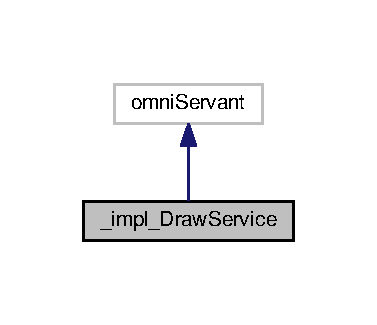
\includegraphics[width=181pt]{class__impl___draw_service__inherit__graph}
\end{center}
\end{figure}


Collaboration diagram for \+\_\+impl\+\_\+\+Draw\+Service\+:
\nopagebreak
\begin{figure}[H]
\begin{center}
\leavevmode
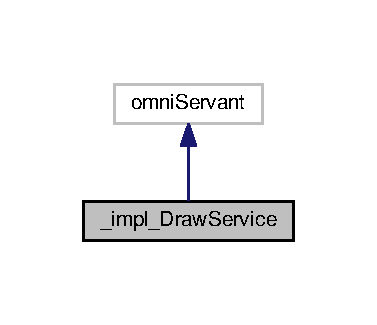
\includegraphics[width=181pt]{class__impl___draw_service__coll__graph}
\end{center}
\end{figure}
\subsection*{Public Member Functions}
\begin{DoxyCompactItemize}
\item 
virtual \hyperlink{class__impl___draw_service_abc5f8fe906c4a25bf7c383522c7de6f0}{$\sim$\+\_\+impl\+\_\+\+Draw\+Service} ()
\item 
virtual \+::C\+O\+R\+B\+A\+::\+Double \hyperlink{class__impl___draw_service_a56f247aa66ce6d19f0efb668bef1c98c}{area} (\+::C\+O\+R\+B\+A\+::\+Long id)=0
\item 
virtual \+::C\+O\+R\+B\+A\+::\+Double \hyperlink{class__impl___draw_service_acea99a5740af9baaaca7e31cf811b1f5}{perimeter} (\+::C\+O\+R\+B\+A\+::\+Long id)=0
\item 
virtual void \hyperlink{class__impl___draw_service_aa5dfb4b031e2f90522da143f3effcf05}{homothetie} (\+::C\+O\+R\+B\+A\+::\+Long id,\+::C\+O\+R\+B\+A\+::\+Double index)=0
\item 
virtual void \hyperlink{class__impl___draw_service_a16a7618df309aa42a6c54db76b288cb8}{translation} (\+::C\+O\+R\+B\+A\+::\+Long id,\+::C\+O\+R\+B\+A\+::\+Double x,\+::C\+O\+R\+B\+A\+::\+Double y)=0
\item 
virtual void \hyperlink{class__impl___draw_service_a3a326593c83412786dec749736471ef9}{rotation} (\+::C\+O\+R\+B\+A\+::\+Long id,\+::C\+O\+R\+B\+A\+::\+Double angle)=0
\item 
virtual void \hyperlink{class__impl___draw_service_aea4e775f321ba6cdc625337001e0bb17}{sym\+Center} (\+::C\+O\+R\+B\+A\+::\+Long id)=0
\item 
virtual void \hyperlink{class__impl___draw_service_a72090bd05cc79fc89fac766aa7d21132}{sym\+Axial} (\+::C\+O\+R\+B\+A\+::\+Long id)=0
\item 
virtual void \hyperlink{class__impl___draw_service_a4e609f28be9ac2f4d15fcc3abdc17270}{add\+Draw} (\+::C\+O\+R\+B\+A\+::\+Long pid,\+::C\+O\+R\+B\+A\+::\+Long cid)=0
\item 
virtual char $\ast$ \hyperlink{class__impl___draw_service_a7b115f6ba7092715c74ad6be39a29a03}{to\+String} (\+::C\+O\+R\+B\+A\+::\+Long id)=0
\item 
virtual \+\_\+\+C\+O\+R\+B\+A\+\_\+\+Boolean \hyperlink{class__impl___draw_service_a12bd1d1156617ee727eb120028728d65}{\+\_\+dispatch} (omni\+Call\+Handle \&)
\end{DoxyCompactItemize}


\subsection{Detailed Description}


Definition at line 1047 of file Petit\+Prince.\+hpp.



\subsection{Constructor \& Destructor Documentation}
\index{\+\_\+impl\+\_\+\+Draw\+Service@{\+\_\+impl\+\_\+\+Draw\+Service}!````~\+\_\+impl\+\_\+\+Draw\+Service@{$\sim$\+\_\+impl\+\_\+\+Draw\+Service}}
\index{````~\+\_\+impl\+\_\+\+Draw\+Service@{$\sim$\+\_\+impl\+\_\+\+Draw\+Service}!\+\_\+impl\+\_\+\+Draw\+Service@{\+\_\+impl\+\_\+\+Draw\+Service}}
\subsubsection[{\texorpdfstring{$\sim$\+\_\+impl\+\_\+\+Draw\+Service()}{~_impl_DrawService()}}]{\setlength{\rightskip}{0pt plus 5cm}virtual \+\_\+impl\+\_\+\+Draw\+Service\+::$\sim$\+\_\+impl\+\_\+\+Draw\+Service (
\begin{DoxyParamCaption}
{}
\end{DoxyParamCaption}
)\hspace{0.3cm}{\ttfamily [virtual]}}\hypertarget{class__impl___draw_service_abc5f8fe906c4a25bf7c383522c7de6f0}{}\label{class__impl___draw_service_abc5f8fe906c4a25bf7c383522c7de6f0}


\subsection{Member Function Documentation}
\index{\+\_\+impl\+\_\+\+Draw\+Service@{\+\_\+impl\+\_\+\+Draw\+Service}!\+\_\+dispatch@{\+\_\+dispatch}}
\index{\+\_\+dispatch@{\+\_\+dispatch}!\+\_\+impl\+\_\+\+Draw\+Service@{\+\_\+impl\+\_\+\+Draw\+Service}}
\subsubsection[{\texorpdfstring{\+\_\+dispatch(omni\+Call\+Handle \&)}{_dispatch(omniCallHandle &)}}]{\setlength{\rightskip}{0pt plus 5cm}virtual \+\_\+\+C\+O\+R\+B\+A\+\_\+\+Boolean \+\_\+impl\+\_\+\+Draw\+Service\+::\+\_\+dispatch (
\begin{DoxyParamCaption}
\item[{omni\+Call\+Handle \&}]{}
\end{DoxyParamCaption}
)\hspace{0.3cm}{\ttfamily [virtual]}}\hypertarget{class__impl___draw_service_a12bd1d1156617ee727eb120028728d65}{}\label{class__impl___draw_service_a12bd1d1156617ee727eb120028728d65}
\index{\+\_\+impl\+\_\+\+Draw\+Service@{\+\_\+impl\+\_\+\+Draw\+Service}!add\+Draw@{add\+Draw}}
\index{add\+Draw@{add\+Draw}!\+\_\+impl\+\_\+\+Draw\+Service@{\+\_\+impl\+\_\+\+Draw\+Service}}
\subsubsection[{\texorpdfstring{add\+Draw(\+::\+C\+O\+R\+B\+A\+::\+Long pid,\+::\+C\+O\+R\+B\+A\+::\+Long cid)=0}{addDraw(::CORBA::Long pid,::CORBA::Long cid)=0}}]{\setlength{\rightskip}{0pt plus 5cm}virtual void \+\_\+impl\+\_\+\+Draw\+Service\+::add\+Draw (
\begin{DoxyParamCaption}
\item[{\+::C\+O\+R\+B\+A\+::\+Long}]{pid, }
\item[{\+::C\+O\+R\+B\+A\+::\+Long}]{cid}
\end{DoxyParamCaption}
)\hspace{0.3cm}{\ttfamily [pure virtual]}}\hypertarget{class__impl___draw_service_a4e609f28be9ac2f4d15fcc3abdc17270}{}\label{class__impl___draw_service_a4e609f28be9ac2f4d15fcc3abdc17270}
\index{\+\_\+impl\+\_\+\+Draw\+Service@{\+\_\+impl\+\_\+\+Draw\+Service}!area@{area}}
\index{area@{area}!\+\_\+impl\+\_\+\+Draw\+Service@{\+\_\+impl\+\_\+\+Draw\+Service}}
\subsubsection[{\texorpdfstring{area(\+::\+C\+O\+R\+B\+A\+::\+Long id)=0}{area(::CORBA::Long id)=0}}]{\setlength{\rightskip}{0pt plus 5cm}virtual \+::C\+O\+R\+B\+A\+::\+Double \+\_\+impl\+\_\+\+Draw\+Service\+::area (
\begin{DoxyParamCaption}
\item[{\+::C\+O\+R\+B\+A\+::\+Long}]{id}
\end{DoxyParamCaption}
)\hspace{0.3cm}{\ttfamily [pure virtual]}}\hypertarget{class__impl___draw_service_a56f247aa66ce6d19f0efb668bef1c98c}{}\label{class__impl___draw_service_a56f247aa66ce6d19f0efb668bef1c98c}
\index{\+\_\+impl\+\_\+\+Draw\+Service@{\+\_\+impl\+\_\+\+Draw\+Service}!homothetie@{homothetie}}
\index{homothetie@{homothetie}!\+\_\+impl\+\_\+\+Draw\+Service@{\+\_\+impl\+\_\+\+Draw\+Service}}
\subsubsection[{\texorpdfstring{homothetie(\+::\+C\+O\+R\+B\+A\+::\+Long id,\+::\+C\+O\+R\+B\+A\+::\+Double index)=0}{homothetie(::CORBA::Long id,::CORBA::Double index)=0}}]{\setlength{\rightskip}{0pt plus 5cm}virtual void \+\_\+impl\+\_\+\+Draw\+Service\+::homothetie (
\begin{DoxyParamCaption}
\item[{\+::C\+O\+R\+B\+A\+::\+Long}]{id, }
\item[{\+::C\+O\+R\+B\+A\+::\+Double}]{index}
\end{DoxyParamCaption}
)\hspace{0.3cm}{\ttfamily [pure virtual]}}\hypertarget{class__impl___draw_service_aa5dfb4b031e2f90522da143f3effcf05}{}\label{class__impl___draw_service_aa5dfb4b031e2f90522da143f3effcf05}
\index{\+\_\+impl\+\_\+\+Draw\+Service@{\+\_\+impl\+\_\+\+Draw\+Service}!perimeter@{perimeter}}
\index{perimeter@{perimeter}!\+\_\+impl\+\_\+\+Draw\+Service@{\+\_\+impl\+\_\+\+Draw\+Service}}
\subsubsection[{\texorpdfstring{perimeter(\+::\+C\+O\+R\+B\+A\+::\+Long id)=0}{perimeter(::CORBA::Long id)=0}}]{\setlength{\rightskip}{0pt plus 5cm}virtual \+::C\+O\+R\+B\+A\+::\+Double \+\_\+impl\+\_\+\+Draw\+Service\+::perimeter (
\begin{DoxyParamCaption}
\item[{\+::C\+O\+R\+B\+A\+::\+Long}]{id}
\end{DoxyParamCaption}
)\hspace{0.3cm}{\ttfamily [pure virtual]}}\hypertarget{class__impl___draw_service_acea99a5740af9baaaca7e31cf811b1f5}{}\label{class__impl___draw_service_acea99a5740af9baaaca7e31cf811b1f5}
\index{\+\_\+impl\+\_\+\+Draw\+Service@{\+\_\+impl\+\_\+\+Draw\+Service}!rotation@{rotation}}
\index{rotation@{rotation}!\+\_\+impl\+\_\+\+Draw\+Service@{\+\_\+impl\+\_\+\+Draw\+Service}}
\subsubsection[{\texorpdfstring{rotation(\+::\+C\+O\+R\+B\+A\+::\+Long id,\+::\+C\+O\+R\+B\+A\+::\+Double angle)=0}{rotation(::CORBA::Long id,::CORBA::Double angle)=0}}]{\setlength{\rightskip}{0pt plus 5cm}virtual void \+\_\+impl\+\_\+\+Draw\+Service\+::rotation (
\begin{DoxyParamCaption}
\item[{\+::C\+O\+R\+B\+A\+::\+Long}]{id, }
\item[{\+::C\+O\+R\+B\+A\+::\+Double}]{angle}
\end{DoxyParamCaption}
)\hspace{0.3cm}{\ttfamily [pure virtual]}}\hypertarget{class__impl___draw_service_a3a326593c83412786dec749736471ef9}{}\label{class__impl___draw_service_a3a326593c83412786dec749736471ef9}
\index{\+\_\+impl\+\_\+\+Draw\+Service@{\+\_\+impl\+\_\+\+Draw\+Service}!sym\+Axial@{sym\+Axial}}
\index{sym\+Axial@{sym\+Axial}!\+\_\+impl\+\_\+\+Draw\+Service@{\+\_\+impl\+\_\+\+Draw\+Service}}
\subsubsection[{\texorpdfstring{sym\+Axial(\+::\+C\+O\+R\+B\+A\+::\+Long id)=0}{symAxial(::CORBA::Long id)=0}}]{\setlength{\rightskip}{0pt plus 5cm}virtual void \+\_\+impl\+\_\+\+Draw\+Service\+::sym\+Axial (
\begin{DoxyParamCaption}
\item[{\+::C\+O\+R\+B\+A\+::\+Long}]{id}
\end{DoxyParamCaption}
)\hspace{0.3cm}{\ttfamily [pure virtual]}}\hypertarget{class__impl___draw_service_a72090bd05cc79fc89fac766aa7d21132}{}\label{class__impl___draw_service_a72090bd05cc79fc89fac766aa7d21132}
\index{\+\_\+impl\+\_\+\+Draw\+Service@{\+\_\+impl\+\_\+\+Draw\+Service}!sym\+Center@{sym\+Center}}
\index{sym\+Center@{sym\+Center}!\+\_\+impl\+\_\+\+Draw\+Service@{\+\_\+impl\+\_\+\+Draw\+Service}}
\subsubsection[{\texorpdfstring{sym\+Center(\+::\+C\+O\+R\+B\+A\+::\+Long id)=0}{symCenter(::CORBA::Long id)=0}}]{\setlength{\rightskip}{0pt plus 5cm}virtual void \+\_\+impl\+\_\+\+Draw\+Service\+::sym\+Center (
\begin{DoxyParamCaption}
\item[{\+::C\+O\+R\+B\+A\+::\+Long}]{id}
\end{DoxyParamCaption}
)\hspace{0.3cm}{\ttfamily [pure virtual]}}\hypertarget{class__impl___draw_service_aea4e775f321ba6cdc625337001e0bb17}{}\label{class__impl___draw_service_aea4e775f321ba6cdc625337001e0bb17}
\index{\+\_\+impl\+\_\+\+Draw\+Service@{\+\_\+impl\+\_\+\+Draw\+Service}!to\+String@{to\+String}}
\index{to\+String@{to\+String}!\+\_\+impl\+\_\+\+Draw\+Service@{\+\_\+impl\+\_\+\+Draw\+Service}}
\subsubsection[{\texorpdfstring{to\+String(\+::\+C\+O\+R\+B\+A\+::\+Long id)=0}{toString(::CORBA::Long id)=0}}]{\setlength{\rightskip}{0pt plus 5cm}virtual char$\ast$ \+\_\+impl\+\_\+\+Draw\+Service\+::to\+String (
\begin{DoxyParamCaption}
\item[{\+::C\+O\+R\+B\+A\+::\+Long}]{id}
\end{DoxyParamCaption}
)\hspace{0.3cm}{\ttfamily [pure virtual]}}\hypertarget{class__impl___draw_service_a7b115f6ba7092715c74ad6be39a29a03}{}\label{class__impl___draw_service_a7b115f6ba7092715c74ad6be39a29a03}
\index{\+\_\+impl\+\_\+\+Draw\+Service@{\+\_\+impl\+\_\+\+Draw\+Service}!translation@{translation}}
\index{translation@{translation}!\+\_\+impl\+\_\+\+Draw\+Service@{\+\_\+impl\+\_\+\+Draw\+Service}}
\subsubsection[{\texorpdfstring{translation(\+::\+C\+O\+R\+B\+A\+::\+Long id,\+::\+C\+O\+R\+B\+A\+::\+Double x,\+::\+C\+O\+R\+B\+A\+::\+Double y)=0}{translation(::CORBA::Long id,::CORBA::Double x,::CORBA::Double y)=0}}]{\setlength{\rightskip}{0pt plus 5cm}virtual void \+\_\+impl\+\_\+\+Draw\+Service\+::translation (
\begin{DoxyParamCaption}
\item[{\+::C\+O\+R\+B\+A\+::\+Long}]{id, }
\item[{\+::C\+O\+R\+B\+A\+::\+Double}]{x, }
\item[{\+::C\+O\+R\+B\+A\+::\+Double}]{y}
\end{DoxyParamCaption}
)\hspace{0.3cm}{\ttfamily [pure virtual]}}\hypertarget{class__impl___draw_service_a16a7618df309aa42a6c54db76b288cb8}{}\label{class__impl___draw_service_a16a7618df309aa42a6c54db76b288cb8}


The documentation for this class was generated from the following file\+:\begin{DoxyCompactItemize}
\item 
hdr/\hyperlink{_petit_prince_8hpp}{Petit\+Prince.\+hpp}\end{DoxyCompactItemize}

\hypertarget{class__impl___petit_prince_service}{}\section{\+\_\+impl\+\_\+\+Petit\+Prince\+Service Class Reference}
\label{class__impl___petit_prince_service}\index{\+\_\+impl\+\_\+\+Petit\+Prince\+Service@{\+\_\+impl\+\_\+\+Petit\+Prince\+Service}}


{\ttfamily \#include $<$Petit\+Prince.\+hpp$>$}



Inheritance diagram for \+\_\+impl\+\_\+\+Petit\+Prince\+Service\+:
\nopagebreak
\begin{figure}[H]
\begin{center}
\leavevmode
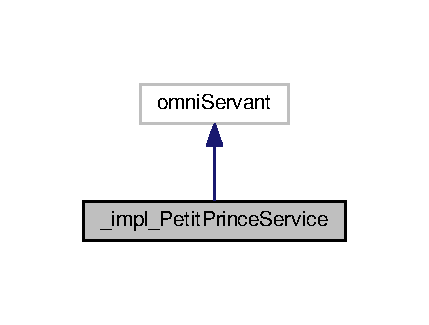
\includegraphics[width=206pt]{class__impl___petit_prince_service__inherit__graph}
\end{center}
\end{figure}


Collaboration diagram for \+\_\+impl\+\_\+\+Petit\+Prince\+Service\+:
\nopagebreak
\begin{figure}[H]
\begin{center}
\leavevmode
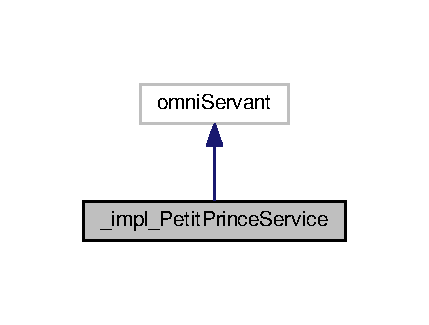
\includegraphics[width=206pt]{class__impl___petit_prince_service__coll__graph}
\end{center}
\end{figure}
\subsection*{Public Member Functions}
\begin{DoxyCompactItemize}
\item 
virtual \hyperlink{class__impl___petit_prince_service_a477c2f68aac99912c47455657764b266}{$\sim$\+\_\+impl\+\_\+\+Petit\+Prince\+Service} ()
\item 
virtual \+::C\+O\+R\+B\+A\+::\+Long \hyperlink{class__impl___petit_prince_service_a7d0f1d9c237b859cba5e5d98ef248069}{create\+Line} (const char $\ast$author, const \+::Petit\+Prince\+::\+Point \&a, const \+::Petit\+Prince\+::\+Point \&b)=0
\item 
virtual \+::C\+O\+R\+B\+A\+::\+Long \hyperlink{class__impl___petit_prince_service_a8b07dfb70c61bb9d6367bacf1a0230d3}{create\+Circle} (const char $\ast$author, const \+::Petit\+Prince\+::\+Point \&center,\+::C\+O\+R\+B\+A\+::\+Double ray)=0
\item 
virtual \+::C\+O\+R\+B\+A\+::\+Long \hyperlink{class__impl___petit_prince_service_ad8fb48af108a078b4ee0a3679a72499f}{create\+Ellipse} (const char $\ast$author, const \+::Petit\+Prince\+::\+Point \&center,\+::C\+O\+R\+B\+A\+::\+Double long\+\_\+ray,\+::C\+O\+R\+B\+A\+::\+Double short\+\_\+ray)=0
\item 
virtual \+::C\+O\+R\+B\+A\+::\+Long \hyperlink{class__impl___petit_prince_service_a89b8c0ca5d95f6712916a5e781f1f9ed}{create\+Polygon} (const char $\ast$author, const \+::Petit\+Prince\+::\+Point\+Seq \&pts)=0
\item 
virtual \hyperlink{class_long_seq}{Long\+Seq} $\ast$ \hyperlink{class__impl___petit_prince_service_af45641fd3b57ebe1debe37abf0550bba}{get\+Draws} (const char $\ast$author)=0
\item 
virtual void \hyperlink{class__impl___petit_prince_service_aa89e2ba56851bcc143f01f8d96fd1e42}{mark\+Draw} (\+::C\+O\+R\+B\+A\+::\+Double mark,\+::C\+O\+R\+B\+A\+::\+Long id)=0
\item 
virtual \+\_\+\+C\+O\+R\+B\+A\+\_\+\+Boolean \hyperlink{class__impl___petit_prince_service_ac4dc7df1a3329636533b195a84932940}{\+\_\+dispatch} (omni\+Call\+Handle \&)
\end{DoxyCompactItemize}


\subsection{Detailed Description}


Definition at line 1210 of file Petit\+Prince.\+hpp.



\subsection{Constructor \& Destructor Documentation}
\index{\+\_\+impl\+\_\+\+Petit\+Prince\+Service@{\+\_\+impl\+\_\+\+Petit\+Prince\+Service}!````~\+\_\+impl\+\_\+\+Petit\+Prince\+Service@{$\sim$\+\_\+impl\+\_\+\+Petit\+Prince\+Service}}
\index{````~\+\_\+impl\+\_\+\+Petit\+Prince\+Service@{$\sim$\+\_\+impl\+\_\+\+Petit\+Prince\+Service}!\+\_\+impl\+\_\+\+Petit\+Prince\+Service@{\+\_\+impl\+\_\+\+Petit\+Prince\+Service}}
\subsubsection[{\texorpdfstring{$\sim$\+\_\+impl\+\_\+\+Petit\+Prince\+Service()}{~_impl_PetitPrinceService()}}]{\setlength{\rightskip}{0pt plus 5cm}virtual \+\_\+impl\+\_\+\+Petit\+Prince\+Service\+::$\sim$\+\_\+impl\+\_\+\+Petit\+Prince\+Service (
\begin{DoxyParamCaption}
{}
\end{DoxyParamCaption}
)\hspace{0.3cm}{\ttfamily [virtual]}}\hypertarget{class__impl___petit_prince_service_a477c2f68aac99912c47455657764b266}{}\label{class__impl___petit_prince_service_a477c2f68aac99912c47455657764b266}


\subsection{Member Function Documentation}
\index{\+\_\+impl\+\_\+\+Petit\+Prince\+Service@{\+\_\+impl\+\_\+\+Petit\+Prince\+Service}!\+\_\+dispatch@{\+\_\+dispatch}}
\index{\+\_\+dispatch@{\+\_\+dispatch}!\+\_\+impl\+\_\+\+Petit\+Prince\+Service@{\+\_\+impl\+\_\+\+Petit\+Prince\+Service}}
\subsubsection[{\texorpdfstring{\+\_\+dispatch(omni\+Call\+Handle \&)}{_dispatch(omniCallHandle &)}}]{\setlength{\rightskip}{0pt plus 5cm}virtual \+\_\+\+C\+O\+R\+B\+A\+\_\+\+Boolean \+\_\+impl\+\_\+\+Petit\+Prince\+Service\+::\+\_\+dispatch (
\begin{DoxyParamCaption}
\item[{omni\+Call\+Handle \&}]{}
\end{DoxyParamCaption}
)\hspace{0.3cm}{\ttfamily [virtual]}}\hypertarget{class__impl___petit_prince_service_ac4dc7df1a3329636533b195a84932940}{}\label{class__impl___petit_prince_service_ac4dc7df1a3329636533b195a84932940}
\index{\+\_\+impl\+\_\+\+Petit\+Prince\+Service@{\+\_\+impl\+\_\+\+Petit\+Prince\+Service}!create\+Circle@{create\+Circle}}
\index{create\+Circle@{create\+Circle}!\+\_\+impl\+\_\+\+Petit\+Prince\+Service@{\+\_\+impl\+\_\+\+Petit\+Prince\+Service}}
\subsubsection[{\texorpdfstring{create\+Circle(const char $\ast$author, const \+::\+Petit\+Prince\+::\+Point \&center,\+::\+C\+O\+R\+B\+A\+::\+Double ray)=0}{createCircle(const char *author, const ::PetitPrince::Point &center,::CORBA::Double ray)=0}}]{\setlength{\rightskip}{0pt plus 5cm}virtual \+::C\+O\+R\+B\+A\+::\+Long \+\_\+impl\+\_\+\+Petit\+Prince\+Service\+::create\+Circle (
\begin{DoxyParamCaption}
\item[{const char $\ast$}]{author, }
\item[{const \+::Petit\+Prince\+::\+Point \&}]{center, }
\item[{\+::C\+O\+R\+B\+A\+::\+Double}]{ray}
\end{DoxyParamCaption}
)\hspace{0.3cm}{\ttfamily [pure virtual]}}\hypertarget{class__impl___petit_prince_service_a8b07dfb70c61bb9d6367bacf1a0230d3}{}\label{class__impl___petit_prince_service_a8b07dfb70c61bb9d6367bacf1a0230d3}
\index{\+\_\+impl\+\_\+\+Petit\+Prince\+Service@{\+\_\+impl\+\_\+\+Petit\+Prince\+Service}!create\+Ellipse@{create\+Ellipse}}
\index{create\+Ellipse@{create\+Ellipse}!\+\_\+impl\+\_\+\+Petit\+Prince\+Service@{\+\_\+impl\+\_\+\+Petit\+Prince\+Service}}
\subsubsection[{\texorpdfstring{create\+Ellipse(const char $\ast$author, const \+::\+Petit\+Prince\+::\+Point \&center,\+::\+C\+O\+R\+B\+A\+::\+Double long\+\_\+ray,\+::\+C\+O\+R\+B\+A\+::\+Double short\+\_\+ray)=0}{createEllipse(const char *author, const ::PetitPrince::Point &center,::CORBA::Double long_ray,::CORBA::Double short_ray)=0}}]{\setlength{\rightskip}{0pt plus 5cm}virtual \+::C\+O\+R\+B\+A\+::\+Long \+\_\+impl\+\_\+\+Petit\+Prince\+Service\+::create\+Ellipse (
\begin{DoxyParamCaption}
\item[{const char $\ast$}]{author, }
\item[{const \+::Petit\+Prince\+::\+Point \&}]{center, }
\item[{\+::C\+O\+R\+B\+A\+::\+Double}]{long\+\_\+ray, }
\item[{\+::C\+O\+R\+B\+A\+::\+Double}]{short\+\_\+ray}
\end{DoxyParamCaption}
)\hspace{0.3cm}{\ttfamily [pure virtual]}}\hypertarget{class__impl___petit_prince_service_ad8fb48af108a078b4ee0a3679a72499f}{}\label{class__impl___petit_prince_service_ad8fb48af108a078b4ee0a3679a72499f}
\index{\+\_\+impl\+\_\+\+Petit\+Prince\+Service@{\+\_\+impl\+\_\+\+Petit\+Prince\+Service}!create\+Line@{create\+Line}}
\index{create\+Line@{create\+Line}!\+\_\+impl\+\_\+\+Petit\+Prince\+Service@{\+\_\+impl\+\_\+\+Petit\+Prince\+Service}}
\subsubsection[{\texorpdfstring{create\+Line(const char $\ast$author, const \+::\+Petit\+Prince\+::\+Point \&a, const \+::\+Petit\+Prince\+::\+Point \&b)=0}{createLine(const char *author, const ::PetitPrince::Point &a, const ::PetitPrince::Point &b)=0}}]{\setlength{\rightskip}{0pt plus 5cm}virtual \+::C\+O\+R\+B\+A\+::\+Long \+\_\+impl\+\_\+\+Petit\+Prince\+Service\+::create\+Line (
\begin{DoxyParamCaption}
\item[{const char $\ast$}]{author, }
\item[{const \+::Petit\+Prince\+::\+Point \&}]{a, }
\item[{const \+::Petit\+Prince\+::\+Point \&}]{b}
\end{DoxyParamCaption}
)\hspace{0.3cm}{\ttfamily [pure virtual]}}\hypertarget{class__impl___petit_prince_service_a7d0f1d9c237b859cba5e5d98ef248069}{}\label{class__impl___petit_prince_service_a7d0f1d9c237b859cba5e5d98ef248069}
\index{\+\_\+impl\+\_\+\+Petit\+Prince\+Service@{\+\_\+impl\+\_\+\+Petit\+Prince\+Service}!create\+Polygon@{create\+Polygon}}
\index{create\+Polygon@{create\+Polygon}!\+\_\+impl\+\_\+\+Petit\+Prince\+Service@{\+\_\+impl\+\_\+\+Petit\+Prince\+Service}}
\subsubsection[{\texorpdfstring{create\+Polygon(const char $\ast$author, const \+::\+Petit\+Prince\+::\+Point\+Seq \&pts)=0}{createPolygon(const char *author, const ::PetitPrince::PointSeq &pts)=0}}]{\setlength{\rightskip}{0pt plus 5cm}virtual \+::C\+O\+R\+B\+A\+::\+Long \+\_\+impl\+\_\+\+Petit\+Prince\+Service\+::create\+Polygon (
\begin{DoxyParamCaption}
\item[{const char $\ast$}]{author, }
\item[{const \+::Petit\+Prince\+::\+Point\+Seq \&}]{pts}
\end{DoxyParamCaption}
)\hspace{0.3cm}{\ttfamily [pure virtual]}}\hypertarget{class__impl___petit_prince_service_a89b8c0ca5d95f6712916a5e781f1f9ed}{}\label{class__impl___petit_prince_service_a89b8c0ca5d95f6712916a5e781f1f9ed}
\index{\+\_\+impl\+\_\+\+Petit\+Prince\+Service@{\+\_\+impl\+\_\+\+Petit\+Prince\+Service}!get\+Draws@{get\+Draws}}
\index{get\+Draws@{get\+Draws}!\+\_\+impl\+\_\+\+Petit\+Prince\+Service@{\+\_\+impl\+\_\+\+Petit\+Prince\+Service}}
\subsubsection[{\texorpdfstring{get\+Draws(const char $\ast$author)=0}{getDraws(const char *author)=0}}]{\setlength{\rightskip}{0pt plus 5cm}virtual {\bf Long\+Seq}$\ast$ \+\_\+impl\+\_\+\+Petit\+Prince\+Service\+::get\+Draws (
\begin{DoxyParamCaption}
\item[{const char $\ast$}]{author}
\end{DoxyParamCaption}
)\hspace{0.3cm}{\ttfamily [pure virtual]}}\hypertarget{class__impl___petit_prince_service_af45641fd3b57ebe1debe37abf0550bba}{}\label{class__impl___petit_prince_service_af45641fd3b57ebe1debe37abf0550bba}
\index{\+\_\+impl\+\_\+\+Petit\+Prince\+Service@{\+\_\+impl\+\_\+\+Petit\+Prince\+Service}!mark\+Draw@{mark\+Draw}}
\index{mark\+Draw@{mark\+Draw}!\+\_\+impl\+\_\+\+Petit\+Prince\+Service@{\+\_\+impl\+\_\+\+Petit\+Prince\+Service}}
\subsubsection[{\texorpdfstring{mark\+Draw(\+::\+C\+O\+R\+B\+A\+::\+Double mark,\+::\+C\+O\+R\+B\+A\+::\+Long id)=0}{markDraw(::CORBA::Double mark,::CORBA::Long id)=0}}]{\setlength{\rightskip}{0pt plus 5cm}virtual void \+\_\+impl\+\_\+\+Petit\+Prince\+Service\+::mark\+Draw (
\begin{DoxyParamCaption}
\item[{\+::C\+O\+R\+B\+A\+::\+Double}]{mark, }
\item[{\+::C\+O\+R\+B\+A\+::\+Long}]{id}
\end{DoxyParamCaption}
)\hspace{0.3cm}{\ttfamily [pure virtual]}}\hypertarget{class__impl___petit_prince_service_aa89e2ba56851bcc143f01f8d96fd1e42}{}\label{class__impl___petit_prince_service_aa89e2ba56851bcc143f01f8d96fd1e42}


The documentation for this class was generated from the following file\+:\begin{DoxyCompactItemize}
\item 
hdr/\hyperlink{_petit_prince_8hpp}{Petit\+Prince.\+hpp}\end{DoxyCompactItemize}

\hypertarget{class__objref___draw_service}{}\section{\+\_\+objref\+\_\+\+Draw\+Service Class Reference}
\label{class__objref___draw_service}\index{\+\_\+objref\+\_\+\+Draw\+Service@{\+\_\+objref\+\_\+\+Draw\+Service}}


{\ttfamily \#include $<$Petit\+Prince.\+hpp$>$}



Inheritance diagram for \+\_\+objref\+\_\+\+Draw\+Service\+:
\nopagebreak
\begin{figure}[H]
\begin{center}
\leavevmode
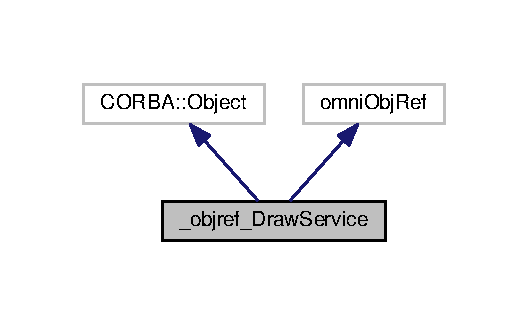
\includegraphics[width=254pt]{class__objref___draw_service__inherit__graph}
\end{center}
\end{figure}


Collaboration diagram for \+\_\+objref\+\_\+\+Draw\+Service\+:
\nopagebreak
\begin{figure}[H]
\begin{center}
\leavevmode
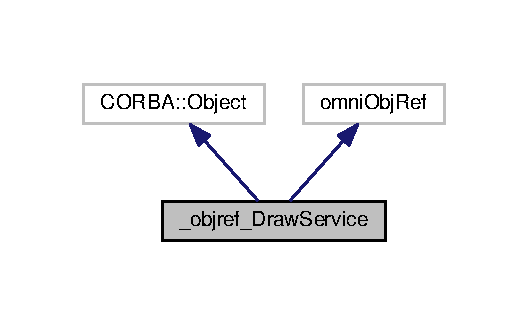
\includegraphics[width=254pt]{class__objref___draw_service__coll__graph}
\end{center}
\end{figure}
\subsection*{Public Member Functions}
\begin{DoxyCompactItemize}
\item 
\+::C\+O\+R\+B\+A\+::\+Double \hyperlink{class__objref___draw_service_a2c3483f409eb3a6a7f8e810e83c33f84}{area} (\+::C\+O\+R\+B\+A\+::\+Long id)
\item 
\+::C\+O\+R\+B\+A\+::\+Double \hyperlink{class__objref___draw_service_afdb653b8fcf7e10a1c3e3953bef0fdd5}{perimeter} (\+::C\+O\+R\+B\+A\+::\+Long id)
\item 
void \hyperlink{class__objref___draw_service_a9994197fccedfac8edc3e23d2209a227}{homothetie} (\+::C\+O\+R\+B\+A\+::\+Long id,\+::C\+O\+R\+B\+A\+::\+Double index)
\item 
void \hyperlink{class__objref___draw_service_a071c62572390b6d20615afdce21adec4}{translation} (\+::C\+O\+R\+B\+A\+::\+Long id,\+::C\+O\+R\+B\+A\+::\+Double x,\+::C\+O\+R\+B\+A\+::\+Double y)
\item 
void \hyperlink{class__objref___draw_service_a1780564038d80177fe9edbcc6667bc1e}{rotation} (\+::C\+O\+R\+B\+A\+::\+Long id,\+::C\+O\+R\+B\+A\+::\+Double angle)
\item 
void \hyperlink{class__objref___draw_service_adbeccf72a76c7584277919e736f7bec2}{sym\+Center} (\+::C\+O\+R\+B\+A\+::\+Long id)
\item 
void \hyperlink{class__objref___draw_service_aa515f8f0c6b6e07e4609f03efb12aa7e}{sym\+Axial} (\+::C\+O\+R\+B\+A\+::\+Long id)
\item 
void \hyperlink{class__objref___draw_service_a1fa9bba40ebcc7726f2fc54fe21719d2}{add\+Draw} (\+::C\+O\+R\+B\+A\+::\+Long pid,\+::C\+O\+R\+B\+A\+::\+Long cid)
\item 
char $\ast$ \hyperlink{class__objref___draw_service_a8fc2d537f125bf90fd1c620e38efb251}{to\+String} (\+::C\+O\+R\+B\+A\+::\+Long id)
\item 
\hyperlink{class__objref___draw_service_aa60d7ece4d50a924e20ea7354e622ddb}{\+\_\+objref\+\_\+\+Draw\+Service} ()
\item 
\hyperlink{class__objref___draw_service_af87c58cc0e9437d7bed172134bf91567}{\+\_\+objref\+\_\+\+Draw\+Service} (omni\+I\+OR $\ast$, omni\+Identity $\ast$)
\end{DoxyCompactItemize}
\subsection*{Protected Member Functions}
\begin{DoxyCompactItemize}
\item 
virtual \hyperlink{class__objref___draw_service_a8f59efe7fc23282519e703262482cec6}{$\sim$\+\_\+objref\+\_\+\+Draw\+Service} ()
\end{DoxyCompactItemize}
\subsection*{Friends}
\begin{DoxyCompactItemize}
\item 
class \hyperlink{class__objref___draw_service_a62bdd6963f13b584c2898676eeb9951d}{Draw\+Service}
\end{DoxyCompactItemize}


\subsection{Constructor \& Destructor Documentation}
\index{\+\_\+objref\+\_\+\+Draw\+Service@{\+\_\+objref\+\_\+\+Draw\+Service}!\+\_\+objref\+\_\+\+Draw\+Service@{\+\_\+objref\+\_\+\+Draw\+Service}}
\index{\+\_\+objref\+\_\+\+Draw\+Service@{\+\_\+objref\+\_\+\+Draw\+Service}!\+\_\+objref\+\_\+\+Draw\+Service@{\+\_\+objref\+\_\+\+Draw\+Service}}
\subsubsection[{\texorpdfstring{\+\_\+objref\+\_\+\+Draw\+Service()}{_objref_DrawService()}}]{\setlength{\rightskip}{0pt plus 5cm}\+\_\+objref\+\_\+\+Draw\+Service\+::\+\_\+objref\+\_\+\+Draw\+Service (
\begin{DoxyParamCaption}
{}
\end{DoxyParamCaption}
)\hspace{0.3cm}{\ttfamily [inline]}}\hypertarget{class__objref___draw_service_aa60d7ece4d50a924e20ea7354e622ddb}{}\label{class__objref___draw_service_aa60d7ece4d50a924e20ea7354e622ddb}
\index{\+\_\+objref\+\_\+\+Draw\+Service@{\+\_\+objref\+\_\+\+Draw\+Service}!\+\_\+objref\+\_\+\+Draw\+Service@{\+\_\+objref\+\_\+\+Draw\+Service}}
\index{\+\_\+objref\+\_\+\+Draw\+Service@{\+\_\+objref\+\_\+\+Draw\+Service}!\+\_\+objref\+\_\+\+Draw\+Service@{\+\_\+objref\+\_\+\+Draw\+Service}}
\subsubsection[{\texorpdfstring{\+\_\+objref\+\_\+\+Draw\+Service(omni\+I\+O\+R $\ast$, omni\+Identity $\ast$)}{_objref_DrawService(omniIOR *, omniIdentity *)}}]{\setlength{\rightskip}{0pt plus 5cm}\+\_\+objref\+\_\+\+Draw\+Service\+::\+\_\+objref\+\_\+\+Draw\+Service (
\begin{DoxyParamCaption}
\item[{omni\+I\+OR $\ast$}]{, }
\item[{omni\+Identity $\ast$}]{}
\end{DoxyParamCaption}
)}\hypertarget{class__objref___draw_service_af87c58cc0e9437d7bed172134bf91567}{}\label{class__objref___draw_service_af87c58cc0e9437d7bed172134bf91567}
\index{\+\_\+objref\+\_\+\+Draw\+Service@{\+\_\+objref\+\_\+\+Draw\+Service}!````~\+\_\+objref\+\_\+\+Draw\+Service@{$\sim$\+\_\+objref\+\_\+\+Draw\+Service}}
\index{````~\+\_\+objref\+\_\+\+Draw\+Service@{$\sim$\+\_\+objref\+\_\+\+Draw\+Service}!\+\_\+objref\+\_\+\+Draw\+Service@{\+\_\+objref\+\_\+\+Draw\+Service}}
\subsubsection[{\texorpdfstring{$\sim$\+\_\+objref\+\_\+\+Draw\+Service()}{~_objref_DrawService()}}]{\setlength{\rightskip}{0pt plus 5cm}virtual \+\_\+objref\+\_\+\+Draw\+Service\+::$\sim$\+\_\+objref\+\_\+\+Draw\+Service (
\begin{DoxyParamCaption}
{}
\end{DoxyParamCaption}
)\hspace{0.3cm}{\ttfamily [protected]}, {\ttfamily [virtual]}}\hypertarget{class__objref___draw_service_a8f59efe7fc23282519e703262482cec6}{}\label{class__objref___draw_service_a8f59efe7fc23282519e703262482cec6}


\subsection{Member Function Documentation}
\index{\+\_\+objref\+\_\+\+Draw\+Service@{\+\_\+objref\+\_\+\+Draw\+Service}!add\+Draw@{add\+Draw}}
\index{add\+Draw@{add\+Draw}!\+\_\+objref\+\_\+\+Draw\+Service@{\+\_\+objref\+\_\+\+Draw\+Service}}
\subsubsection[{\texorpdfstring{add\+Draw(\+::\+C\+O\+R\+B\+A\+::\+Long pid,\+::\+C\+O\+R\+B\+A\+::\+Long cid)}{addDraw(::CORBA::Long pid,::CORBA::Long cid)}}]{\setlength{\rightskip}{0pt plus 5cm}void \+\_\+objref\+\_\+\+Draw\+Service\+::add\+Draw (
\begin{DoxyParamCaption}
\item[{\+::C\+O\+R\+B\+A\+::\+Long}]{pid, }
\item[{\+::C\+O\+R\+B\+A\+::\+Long}]{cid}
\end{DoxyParamCaption}
)}\hypertarget{class__objref___draw_service_a1fa9bba40ebcc7726f2fc54fe21719d2}{}\label{class__objref___draw_service_a1fa9bba40ebcc7726f2fc54fe21719d2}
\index{\+\_\+objref\+\_\+\+Draw\+Service@{\+\_\+objref\+\_\+\+Draw\+Service}!area@{area}}
\index{area@{area}!\+\_\+objref\+\_\+\+Draw\+Service@{\+\_\+objref\+\_\+\+Draw\+Service}}
\subsubsection[{\texorpdfstring{area(\+::\+C\+O\+R\+B\+A\+::\+Long id)}{area(::CORBA::Long id)}}]{\setlength{\rightskip}{0pt plus 5cm}\+::C\+O\+R\+B\+A\+::\+Double \+\_\+objref\+\_\+\+Draw\+Service\+::area (
\begin{DoxyParamCaption}
\item[{\+::C\+O\+R\+B\+A\+::\+Long}]{id}
\end{DoxyParamCaption}
)}\hypertarget{class__objref___draw_service_a2c3483f409eb3a6a7f8e810e83c33f84}{}\label{class__objref___draw_service_a2c3483f409eb3a6a7f8e810e83c33f84}
\index{\+\_\+objref\+\_\+\+Draw\+Service@{\+\_\+objref\+\_\+\+Draw\+Service}!homothetie@{homothetie}}
\index{homothetie@{homothetie}!\+\_\+objref\+\_\+\+Draw\+Service@{\+\_\+objref\+\_\+\+Draw\+Service}}
\subsubsection[{\texorpdfstring{homothetie(\+::\+C\+O\+R\+B\+A\+::\+Long id,\+::\+C\+O\+R\+B\+A\+::\+Double index)}{homothetie(::CORBA::Long id,::CORBA::Double index)}}]{\setlength{\rightskip}{0pt plus 5cm}void \+\_\+objref\+\_\+\+Draw\+Service\+::homothetie (
\begin{DoxyParamCaption}
\item[{\+::C\+O\+R\+B\+A\+::\+Long}]{id, }
\item[{\+::C\+O\+R\+B\+A\+::\+Double}]{index}
\end{DoxyParamCaption}
)}\hypertarget{class__objref___draw_service_a9994197fccedfac8edc3e23d2209a227}{}\label{class__objref___draw_service_a9994197fccedfac8edc3e23d2209a227}
\index{\+\_\+objref\+\_\+\+Draw\+Service@{\+\_\+objref\+\_\+\+Draw\+Service}!perimeter@{perimeter}}
\index{perimeter@{perimeter}!\+\_\+objref\+\_\+\+Draw\+Service@{\+\_\+objref\+\_\+\+Draw\+Service}}
\subsubsection[{\texorpdfstring{perimeter(\+::\+C\+O\+R\+B\+A\+::\+Long id)}{perimeter(::CORBA::Long id)}}]{\setlength{\rightskip}{0pt plus 5cm}\+::C\+O\+R\+B\+A\+::\+Double \+\_\+objref\+\_\+\+Draw\+Service\+::perimeter (
\begin{DoxyParamCaption}
\item[{\+::C\+O\+R\+B\+A\+::\+Long}]{id}
\end{DoxyParamCaption}
)}\hypertarget{class__objref___draw_service_afdb653b8fcf7e10a1c3e3953bef0fdd5}{}\label{class__objref___draw_service_afdb653b8fcf7e10a1c3e3953bef0fdd5}
\index{\+\_\+objref\+\_\+\+Draw\+Service@{\+\_\+objref\+\_\+\+Draw\+Service}!rotation@{rotation}}
\index{rotation@{rotation}!\+\_\+objref\+\_\+\+Draw\+Service@{\+\_\+objref\+\_\+\+Draw\+Service}}
\subsubsection[{\texorpdfstring{rotation(\+::\+C\+O\+R\+B\+A\+::\+Long id,\+::\+C\+O\+R\+B\+A\+::\+Double angle)}{rotation(::CORBA::Long id,::CORBA::Double angle)}}]{\setlength{\rightskip}{0pt plus 5cm}void \+\_\+objref\+\_\+\+Draw\+Service\+::rotation (
\begin{DoxyParamCaption}
\item[{\+::C\+O\+R\+B\+A\+::\+Long}]{id, }
\item[{\+::C\+O\+R\+B\+A\+::\+Double}]{angle}
\end{DoxyParamCaption}
)}\hypertarget{class__objref___draw_service_a1780564038d80177fe9edbcc6667bc1e}{}\label{class__objref___draw_service_a1780564038d80177fe9edbcc6667bc1e}
\index{\+\_\+objref\+\_\+\+Draw\+Service@{\+\_\+objref\+\_\+\+Draw\+Service}!sym\+Axial@{sym\+Axial}}
\index{sym\+Axial@{sym\+Axial}!\+\_\+objref\+\_\+\+Draw\+Service@{\+\_\+objref\+\_\+\+Draw\+Service}}
\subsubsection[{\texorpdfstring{sym\+Axial(\+::\+C\+O\+R\+B\+A\+::\+Long id)}{symAxial(::CORBA::Long id)}}]{\setlength{\rightskip}{0pt plus 5cm}void \+\_\+objref\+\_\+\+Draw\+Service\+::sym\+Axial (
\begin{DoxyParamCaption}
\item[{\+::C\+O\+R\+B\+A\+::\+Long}]{id}
\end{DoxyParamCaption}
)}\hypertarget{class__objref___draw_service_aa515f8f0c6b6e07e4609f03efb12aa7e}{}\label{class__objref___draw_service_aa515f8f0c6b6e07e4609f03efb12aa7e}
\index{\+\_\+objref\+\_\+\+Draw\+Service@{\+\_\+objref\+\_\+\+Draw\+Service}!sym\+Center@{sym\+Center}}
\index{sym\+Center@{sym\+Center}!\+\_\+objref\+\_\+\+Draw\+Service@{\+\_\+objref\+\_\+\+Draw\+Service}}
\subsubsection[{\texorpdfstring{sym\+Center(\+::\+C\+O\+R\+B\+A\+::\+Long id)}{symCenter(::CORBA::Long id)}}]{\setlength{\rightskip}{0pt plus 5cm}void \+\_\+objref\+\_\+\+Draw\+Service\+::sym\+Center (
\begin{DoxyParamCaption}
\item[{\+::C\+O\+R\+B\+A\+::\+Long}]{id}
\end{DoxyParamCaption}
)}\hypertarget{class__objref___draw_service_adbeccf72a76c7584277919e736f7bec2}{}\label{class__objref___draw_service_adbeccf72a76c7584277919e736f7bec2}
\index{\+\_\+objref\+\_\+\+Draw\+Service@{\+\_\+objref\+\_\+\+Draw\+Service}!to\+String@{to\+String}}
\index{to\+String@{to\+String}!\+\_\+objref\+\_\+\+Draw\+Service@{\+\_\+objref\+\_\+\+Draw\+Service}}
\subsubsection[{\texorpdfstring{to\+String(\+::\+C\+O\+R\+B\+A\+::\+Long id)}{toString(::CORBA::Long id)}}]{\setlength{\rightskip}{0pt plus 5cm}char$\ast$ \+\_\+objref\+\_\+\+Draw\+Service\+::to\+String (
\begin{DoxyParamCaption}
\item[{\+::C\+O\+R\+B\+A\+::\+Long}]{id}
\end{DoxyParamCaption}
)}\hypertarget{class__objref___draw_service_a8fc2d537f125bf90fd1c620e38efb251}{}\label{class__objref___draw_service_a8fc2d537f125bf90fd1c620e38efb251}
\index{\+\_\+objref\+\_\+\+Draw\+Service@{\+\_\+objref\+\_\+\+Draw\+Service}!translation@{translation}}
\index{translation@{translation}!\+\_\+objref\+\_\+\+Draw\+Service@{\+\_\+objref\+\_\+\+Draw\+Service}}
\subsubsection[{\texorpdfstring{translation(\+::\+C\+O\+R\+B\+A\+::\+Long id,\+::\+C\+O\+R\+B\+A\+::\+Double x,\+::\+C\+O\+R\+B\+A\+::\+Double y)}{translation(::CORBA::Long id,::CORBA::Double x,::CORBA::Double y)}}]{\setlength{\rightskip}{0pt plus 5cm}void \+\_\+objref\+\_\+\+Draw\+Service\+::translation (
\begin{DoxyParamCaption}
\item[{\+::C\+O\+R\+B\+A\+::\+Long}]{id, }
\item[{\+::C\+O\+R\+B\+A\+::\+Double}]{x, }
\item[{\+::C\+O\+R\+B\+A\+::\+Double}]{y}
\end{DoxyParamCaption}
)}\hypertarget{class__objref___draw_service_a071c62572390b6d20615afdce21adec4}{}\label{class__objref___draw_service_a071c62572390b6d20615afdce21adec4}


\subsection{Friends And Related Function Documentation}
\index{\+\_\+objref\+\_\+\+Draw\+Service@{\+\_\+objref\+\_\+\+Draw\+Service}!Draw\+Service@{Draw\+Service}}
\index{Draw\+Service@{Draw\+Service}!\+\_\+objref\+\_\+\+Draw\+Service@{\+\_\+objref\+\_\+\+Draw\+Service}}
\subsubsection[{\texorpdfstring{Draw\+Service}{DrawService}}]{\setlength{\rightskip}{0pt plus 5cm}friend class {\bf Draw\+Service}\hspace{0.3cm}{\ttfamily [friend]}}\hypertarget{class__objref___draw_service_a62bdd6963f13b584c2898676eeb9951d}{}\label{class__objref___draw_service_a62bdd6963f13b584c2898676eeb9951d}


The documentation for this class was generated from the following file\+:\begin{DoxyCompactItemize}
\item 
hdr/\hyperlink{_petit_prince_8hpp}{Petit\+Prince.\+hpp}\end{DoxyCompactItemize}

\hypertarget{class__objref___petit_prince_service}{}\section{\+\_\+objref\+\_\+\+Petit\+Prince\+Service Class Reference}
\label{class__objref___petit_prince_service}\index{\+\_\+objref\+\_\+\+Petit\+Prince\+Service@{\+\_\+objref\+\_\+\+Petit\+Prince\+Service}}


{\ttfamily \#include $<$Petit\+Prince.\+hpp$>$}



Inheritance diagram for \+\_\+objref\+\_\+\+Petit\+Prince\+Service\+:
\nopagebreak
\begin{figure}[H]
\begin{center}
\leavevmode
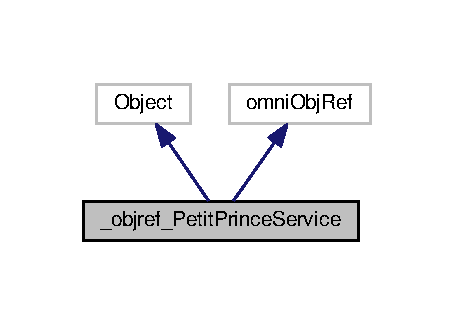
\includegraphics[width=218pt]{class__objref___petit_prince_service__inherit__graph}
\end{center}
\end{figure}


Collaboration diagram for \+\_\+objref\+\_\+\+Petit\+Prince\+Service\+:
\nopagebreak
\begin{figure}[H]
\begin{center}
\leavevmode
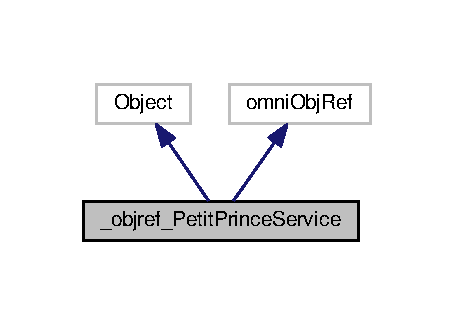
\includegraphics[width=218pt]{class__objref___petit_prince_service__coll__graph}
\end{center}
\end{figure}
\subsection*{Public Member Functions}
\begin{DoxyCompactItemize}
\item 
\+::C\+O\+R\+B\+A\+::\+Long \hyperlink{class__objref___petit_prince_service_a4a5386891a5ef1e372cd31d2a95406af}{create\+Line} (const char $\ast$author, const \+::Petit\+Prince\+::\+Point \&a, const \+::Petit\+Prince\+::\+Point \&b)
\item 
\+::C\+O\+R\+B\+A\+::\+Long \hyperlink{class__objref___petit_prince_service_a5cbe92155f6bdefee2c940a5b14c1c1c}{create\+Circle} (const char $\ast$author, const \+::Petit\+Prince\+::\+Point \&center,\+::C\+O\+R\+B\+A\+::\+Double ray)
\item 
\+::C\+O\+R\+B\+A\+::\+Long \hyperlink{class__objref___petit_prince_service_aac03628fa5351834885765b5da57ba59}{create\+Ellipse} (const char $\ast$author, const \+::Petit\+Prince\+::\+Point \&center,\+::C\+O\+R\+B\+A\+::\+Double long\+\_\+ray,\+::C\+O\+R\+B\+A\+::\+Double short\+\_\+ray)
\item 
\+::C\+O\+R\+B\+A\+::\+Long \hyperlink{class__objref___petit_prince_service_ae05ed84a30f239d63203bd05109b044a}{create\+Polygon} (const char $\ast$author, const \+::Petit\+Prince\+::\+Point\+Seq \&pts)
\item 
\hyperlink{class_long_seq}{Long\+Seq} $\ast$ \hyperlink{class__objref___petit_prince_service_ad9c13910b354fcd183567d42d78d4db3}{get\+Draws} (const char $\ast$author)
\item 
void \hyperlink{class__objref___petit_prince_service_a2bbaeb6486eec446ae07529c99ca5598}{mark\+Draw} (\+::C\+O\+R\+B\+A\+::\+Double mark,\+::C\+O\+R\+B\+A\+::\+Long id)
\item 
\hyperlink{class__objref___petit_prince_service_a7d5aac87fd2840a8f73b60f6f3f05251}{\+\_\+objref\+\_\+\+Petit\+Prince\+Service} ()
\item 
\hyperlink{class__objref___petit_prince_service_ad866a23da1ed08c867b37697565a4e7e}{\+\_\+objref\+\_\+\+Petit\+Prince\+Service} (omni\+I\+OR $\ast$, omni\+Identity $\ast$)
\end{DoxyCompactItemize}
\subsection*{Protected Member Functions}
\begin{DoxyCompactItemize}
\item 
virtual \hyperlink{class__objref___petit_prince_service_aecc6cc3b5c1bfb4ec356337ac550e89b}{$\sim$\+\_\+objref\+\_\+\+Petit\+Prince\+Service} ()
\end{DoxyCompactItemize}
\subsection*{Friends}
\begin{DoxyCompactItemize}
\item 
class \hyperlink{class__objref___petit_prince_service_aeeb7570b0f964a6b6a3eb6cd728fddd0}{Petit\+Prince\+Service}
\end{DoxyCompactItemize}


\subsection{Detailed Description}


Definition at line 1172 of file Petit\+Prince.\+hpp.



\subsection{Constructor \& Destructor Documentation}
\index{\+\_\+objref\+\_\+\+Petit\+Prince\+Service@{\+\_\+objref\+\_\+\+Petit\+Prince\+Service}!\+\_\+objref\+\_\+\+Petit\+Prince\+Service@{\+\_\+objref\+\_\+\+Petit\+Prince\+Service}}
\index{\+\_\+objref\+\_\+\+Petit\+Prince\+Service@{\+\_\+objref\+\_\+\+Petit\+Prince\+Service}!\+\_\+objref\+\_\+\+Petit\+Prince\+Service@{\+\_\+objref\+\_\+\+Petit\+Prince\+Service}}
\subsubsection[{\texorpdfstring{\+\_\+objref\+\_\+\+Petit\+Prince\+Service()}{_objref_PetitPrinceService()}}]{\setlength{\rightskip}{0pt plus 5cm}\+\_\+objref\+\_\+\+Petit\+Prince\+Service\+::\+\_\+objref\+\_\+\+Petit\+Prince\+Service (
\begin{DoxyParamCaption}
{}
\end{DoxyParamCaption}
)\hspace{0.3cm}{\ttfamily [inline]}}\hypertarget{class__objref___petit_prince_service_a7d5aac87fd2840a8f73b60f6f3f05251}{}\label{class__objref___petit_prince_service_a7d5aac87fd2840a8f73b60f6f3f05251}


Definition at line 1184 of file Petit\+Prince.\+hpp.

\index{\+\_\+objref\+\_\+\+Petit\+Prince\+Service@{\+\_\+objref\+\_\+\+Petit\+Prince\+Service}!\+\_\+objref\+\_\+\+Petit\+Prince\+Service@{\+\_\+objref\+\_\+\+Petit\+Prince\+Service}}
\index{\+\_\+objref\+\_\+\+Petit\+Prince\+Service@{\+\_\+objref\+\_\+\+Petit\+Prince\+Service}!\+\_\+objref\+\_\+\+Petit\+Prince\+Service@{\+\_\+objref\+\_\+\+Petit\+Prince\+Service}}
\subsubsection[{\texorpdfstring{\+\_\+objref\+\_\+\+Petit\+Prince\+Service(omni\+I\+O\+R $\ast$, omni\+Identity $\ast$)}{_objref_PetitPrinceService(omniIOR *, omniIdentity *)}}]{\setlength{\rightskip}{0pt plus 5cm}\+\_\+objref\+\_\+\+Petit\+Prince\+Service\+::\+\_\+objref\+\_\+\+Petit\+Prince\+Service (
\begin{DoxyParamCaption}
\item[{omni\+I\+OR $\ast$}]{, }
\item[{omni\+Identity $\ast$}]{}
\end{DoxyParamCaption}
)}\hypertarget{class__objref___petit_prince_service_ad866a23da1ed08c867b37697565a4e7e}{}\label{class__objref___petit_prince_service_ad866a23da1ed08c867b37697565a4e7e}
\index{\+\_\+objref\+\_\+\+Petit\+Prince\+Service@{\+\_\+objref\+\_\+\+Petit\+Prince\+Service}!````~\+\_\+objref\+\_\+\+Petit\+Prince\+Service@{$\sim$\+\_\+objref\+\_\+\+Petit\+Prince\+Service}}
\index{````~\+\_\+objref\+\_\+\+Petit\+Prince\+Service@{$\sim$\+\_\+objref\+\_\+\+Petit\+Prince\+Service}!\+\_\+objref\+\_\+\+Petit\+Prince\+Service@{\+\_\+objref\+\_\+\+Petit\+Prince\+Service}}
\subsubsection[{\texorpdfstring{$\sim$\+\_\+objref\+\_\+\+Petit\+Prince\+Service()}{~_objref_PetitPrinceService()}}]{\setlength{\rightskip}{0pt plus 5cm}virtual \+\_\+objref\+\_\+\+Petit\+Prince\+Service\+::$\sim$\+\_\+objref\+\_\+\+Petit\+Prince\+Service (
\begin{DoxyParamCaption}
{}
\end{DoxyParamCaption}
)\hspace{0.3cm}{\ttfamily [protected]}, {\ttfamily [virtual]}}\hypertarget{class__objref___petit_prince_service_aecc6cc3b5c1bfb4ec356337ac550e89b}{}\label{class__objref___petit_prince_service_aecc6cc3b5c1bfb4ec356337ac550e89b}


\subsection{Member Function Documentation}
\index{\+\_\+objref\+\_\+\+Petit\+Prince\+Service@{\+\_\+objref\+\_\+\+Petit\+Prince\+Service}!create\+Circle@{create\+Circle}}
\index{create\+Circle@{create\+Circle}!\+\_\+objref\+\_\+\+Petit\+Prince\+Service@{\+\_\+objref\+\_\+\+Petit\+Prince\+Service}}
\subsubsection[{\texorpdfstring{create\+Circle(const char $\ast$author, const \+::\+Petit\+Prince\+::\+Point \&center,\+::\+C\+O\+R\+B\+A\+::\+Double ray)}{createCircle(const char *author, const ::PetitPrince::Point &center,::CORBA::Double ray)}}]{\setlength{\rightskip}{0pt plus 5cm}\+::C\+O\+R\+B\+A\+::\+Long \+\_\+objref\+\_\+\+Petit\+Prince\+Service\+::create\+Circle (
\begin{DoxyParamCaption}
\item[{const char $\ast$}]{author, }
\item[{const \+::Petit\+Prince\+::\+Point \&}]{center, }
\item[{\+::C\+O\+R\+B\+A\+::\+Double}]{ray}
\end{DoxyParamCaption}
)}\hypertarget{class__objref___petit_prince_service_a5cbe92155f6bdefee2c940a5b14c1c1c}{}\label{class__objref___petit_prince_service_a5cbe92155f6bdefee2c940a5b14c1c1c}
\index{\+\_\+objref\+\_\+\+Petit\+Prince\+Service@{\+\_\+objref\+\_\+\+Petit\+Prince\+Service}!create\+Ellipse@{create\+Ellipse}}
\index{create\+Ellipse@{create\+Ellipse}!\+\_\+objref\+\_\+\+Petit\+Prince\+Service@{\+\_\+objref\+\_\+\+Petit\+Prince\+Service}}
\subsubsection[{\texorpdfstring{create\+Ellipse(const char $\ast$author, const \+::\+Petit\+Prince\+::\+Point \&center,\+::\+C\+O\+R\+B\+A\+::\+Double long\+\_\+ray,\+::\+C\+O\+R\+B\+A\+::\+Double short\+\_\+ray)}{createEllipse(const char *author, const ::PetitPrince::Point &center,::CORBA::Double long_ray,::CORBA::Double short_ray)}}]{\setlength{\rightskip}{0pt plus 5cm}\+::C\+O\+R\+B\+A\+::\+Long \+\_\+objref\+\_\+\+Petit\+Prince\+Service\+::create\+Ellipse (
\begin{DoxyParamCaption}
\item[{const char $\ast$}]{author, }
\item[{const \+::Petit\+Prince\+::\+Point \&}]{center, }
\item[{\+::C\+O\+R\+B\+A\+::\+Double}]{long\+\_\+ray, }
\item[{\+::C\+O\+R\+B\+A\+::\+Double}]{short\+\_\+ray}
\end{DoxyParamCaption}
)}\hypertarget{class__objref___petit_prince_service_aac03628fa5351834885765b5da57ba59}{}\label{class__objref___petit_prince_service_aac03628fa5351834885765b5da57ba59}
\index{\+\_\+objref\+\_\+\+Petit\+Prince\+Service@{\+\_\+objref\+\_\+\+Petit\+Prince\+Service}!create\+Line@{create\+Line}}
\index{create\+Line@{create\+Line}!\+\_\+objref\+\_\+\+Petit\+Prince\+Service@{\+\_\+objref\+\_\+\+Petit\+Prince\+Service}}
\subsubsection[{\texorpdfstring{create\+Line(const char $\ast$author, const \+::\+Petit\+Prince\+::\+Point \&a, const \+::\+Petit\+Prince\+::\+Point \&b)}{createLine(const char *author, const ::PetitPrince::Point &a, const ::PetitPrince::Point &b)}}]{\setlength{\rightskip}{0pt plus 5cm}\+::C\+O\+R\+B\+A\+::\+Long \+\_\+objref\+\_\+\+Petit\+Prince\+Service\+::create\+Line (
\begin{DoxyParamCaption}
\item[{const char $\ast$}]{author, }
\item[{const \+::Petit\+Prince\+::\+Point \&}]{a, }
\item[{const \+::Petit\+Prince\+::\+Point \&}]{b}
\end{DoxyParamCaption}
)}\hypertarget{class__objref___petit_prince_service_a4a5386891a5ef1e372cd31d2a95406af}{}\label{class__objref___petit_prince_service_a4a5386891a5ef1e372cd31d2a95406af}
\index{\+\_\+objref\+\_\+\+Petit\+Prince\+Service@{\+\_\+objref\+\_\+\+Petit\+Prince\+Service}!create\+Polygon@{create\+Polygon}}
\index{create\+Polygon@{create\+Polygon}!\+\_\+objref\+\_\+\+Petit\+Prince\+Service@{\+\_\+objref\+\_\+\+Petit\+Prince\+Service}}
\subsubsection[{\texorpdfstring{create\+Polygon(const char $\ast$author, const \+::\+Petit\+Prince\+::\+Point\+Seq \&pts)}{createPolygon(const char *author, const ::PetitPrince::PointSeq &pts)}}]{\setlength{\rightskip}{0pt plus 5cm}\+::C\+O\+R\+B\+A\+::\+Long \+\_\+objref\+\_\+\+Petit\+Prince\+Service\+::create\+Polygon (
\begin{DoxyParamCaption}
\item[{const char $\ast$}]{author, }
\item[{const \+::Petit\+Prince\+::\+Point\+Seq \&}]{pts}
\end{DoxyParamCaption}
)}\hypertarget{class__objref___petit_prince_service_ae05ed84a30f239d63203bd05109b044a}{}\label{class__objref___petit_prince_service_ae05ed84a30f239d63203bd05109b044a}
\index{\+\_\+objref\+\_\+\+Petit\+Prince\+Service@{\+\_\+objref\+\_\+\+Petit\+Prince\+Service}!get\+Draws@{get\+Draws}}
\index{get\+Draws@{get\+Draws}!\+\_\+objref\+\_\+\+Petit\+Prince\+Service@{\+\_\+objref\+\_\+\+Petit\+Prince\+Service}}
\subsubsection[{\texorpdfstring{get\+Draws(const char $\ast$author)}{getDraws(const char *author)}}]{\setlength{\rightskip}{0pt plus 5cm}{\bf Long\+Seq}$\ast$ \+\_\+objref\+\_\+\+Petit\+Prince\+Service\+::get\+Draws (
\begin{DoxyParamCaption}
\item[{const char $\ast$}]{author}
\end{DoxyParamCaption}
)}\hypertarget{class__objref___petit_prince_service_ad9c13910b354fcd183567d42d78d4db3}{}\label{class__objref___petit_prince_service_ad9c13910b354fcd183567d42d78d4db3}
\index{\+\_\+objref\+\_\+\+Petit\+Prince\+Service@{\+\_\+objref\+\_\+\+Petit\+Prince\+Service}!mark\+Draw@{mark\+Draw}}
\index{mark\+Draw@{mark\+Draw}!\+\_\+objref\+\_\+\+Petit\+Prince\+Service@{\+\_\+objref\+\_\+\+Petit\+Prince\+Service}}
\subsubsection[{\texorpdfstring{mark\+Draw(\+::\+C\+O\+R\+B\+A\+::\+Double mark,\+::\+C\+O\+R\+B\+A\+::\+Long id)}{markDraw(::CORBA::Double mark,::CORBA::Long id)}}]{\setlength{\rightskip}{0pt plus 5cm}void \+\_\+objref\+\_\+\+Petit\+Prince\+Service\+::mark\+Draw (
\begin{DoxyParamCaption}
\item[{\+::C\+O\+R\+B\+A\+::\+Double}]{mark, }
\item[{\+::C\+O\+R\+B\+A\+::\+Long}]{id}
\end{DoxyParamCaption}
)}\hypertarget{class__objref___petit_prince_service_a2bbaeb6486eec446ae07529c99ca5598}{}\label{class__objref___petit_prince_service_a2bbaeb6486eec446ae07529c99ca5598}


\subsection{Friends And Related Function Documentation}
\index{\+\_\+objref\+\_\+\+Petit\+Prince\+Service@{\+\_\+objref\+\_\+\+Petit\+Prince\+Service}!Petit\+Prince\+Service@{Petit\+Prince\+Service}}
\index{Petit\+Prince\+Service@{Petit\+Prince\+Service}!\+\_\+objref\+\_\+\+Petit\+Prince\+Service@{\+\_\+objref\+\_\+\+Petit\+Prince\+Service}}
\subsubsection[{\texorpdfstring{Petit\+Prince\+Service}{PetitPrinceService}}]{\setlength{\rightskip}{0pt plus 5cm}friend class {\bf Petit\+Prince\+Service}\hspace{0.3cm}{\ttfamily [friend]}}\hypertarget{class__objref___petit_prince_service_aeeb7570b0f964a6b6a3eb6cd728fddd0}{}\label{class__objref___petit_prince_service_aeeb7570b0f964a6b6a3eb6cd728fddd0}


Definition at line 1198 of file Petit\+Prince.\+hpp.



The documentation for this class was generated from the following file\+:\begin{DoxyCompactItemize}
\item 
hdr/\hyperlink{_petit_prince_8hpp}{Petit\+Prince.\+hpp}\end{DoxyCompactItemize}

\hypertarget{class__pof___draw_service}{}\section{\+\_\+pof\+\_\+\+Draw\+Service Class Reference}
\label{class__pof___draw_service}\index{\+\_\+pof\+\_\+\+Draw\+Service@{\+\_\+pof\+\_\+\+Draw\+Service}}


{\ttfamily \#include $<$Petit\+Prince.\+hpp$>$}



Inheritance diagram for \+\_\+pof\+\_\+\+Draw\+Service\+:
\nopagebreak
\begin{figure}[H]
\begin{center}
\leavevmode
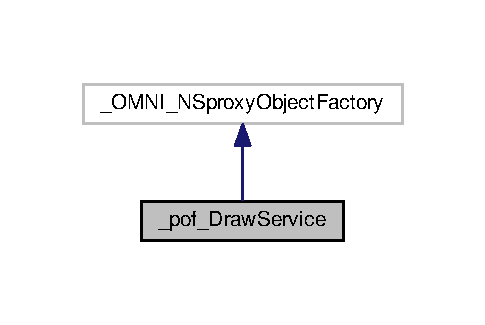
\includegraphics[width=233pt]{class__pof___draw_service__inherit__graph}
\end{center}
\end{figure}


Collaboration diagram for \+\_\+pof\+\_\+\+Draw\+Service\+:
\nopagebreak
\begin{figure}[H]
\begin{center}
\leavevmode
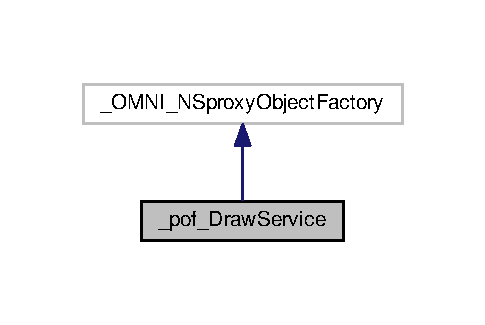
\includegraphics[width=233pt]{class__pof___draw_service__coll__graph}
\end{center}
\end{figure}
\subsection*{Public Member Functions}
\begin{DoxyCompactItemize}
\item 
\hyperlink{class__pof___draw_service_aee04921a7d18e0092ee3eb65cc19fac0}{\+\_\+pof\+\_\+\+Draw\+Service} ()
\item 
virtual \hyperlink{class__pof___draw_service_a8eaecc74531d24fed260cb30c752798b}{$\sim$\+\_\+pof\+\_\+\+Draw\+Service} ()
\item 
virtual omni\+Obj\+Ref $\ast$ \hyperlink{class__pof___draw_service_a11e4f893d46b58731f8ea17ffee147b8}{new\+Obj\+Ref} (omni\+I\+OR $\ast$, omni\+Identity $\ast$)
\item 
virtual \+\_\+\+C\+O\+R\+B\+A\+\_\+\+Boolean \hyperlink{class__pof___draw_service_a6d03d31287dce5a319832d45d736466a}{is\+\_\+a} (const char $\ast$) const 
\end{DoxyCompactItemize}


\subsection{Constructor \& Destructor Documentation}
\index{\+\_\+pof\+\_\+\+Draw\+Service@{\+\_\+pof\+\_\+\+Draw\+Service}!\+\_\+pof\+\_\+\+Draw\+Service@{\+\_\+pof\+\_\+\+Draw\+Service}}
\index{\+\_\+pof\+\_\+\+Draw\+Service@{\+\_\+pof\+\_\+\+Draw\+Service}!\+\_\+pof\+\_\+\+Draw\+Service@{\+\_\+pof\+\_\+\+Draw\+Service}}
\subsubsection[{\texorpdfstring{\+\_\+pof\+\_\+\+Draw\+Service()}{_pof_DrawService()}}]{\setlength{\rightskip}{0pt plus 5cm}\+\_\+pof\+\_\+\+Draw\+Service\+::\+\_\+pof\+\_\+\+Draw\+Service (
\begin{DoxyParamCaption}
{}
\end{DoxyParamCaption}
)\hspace{0.3cm}{\ttfamily [inline]}}\hypertarget{class__pof___draw_service_aee04921a7d18e0092ee3eb65cc19fac0}{}\label{class__pof___draw_service_aee04921a7d18e0092ee3eb65cc19fac0}
\index{\+\_\+pof\+\_\+\+Draw\+Service@{\+\_\+pof\+\_\+\+Draw\+Service}!````~\+\_\+pof\+\_\+\+Draw\+Service@{$\sim$\+\_\+pof\+\_\+\+Draw\+Service}}
\index{````~\+\_\+pof\+\_\+\+Draw\+Service@{$\sim$\+\_\+pof\+\_\+\+Draw\+Service}!\+\_\+pof\+\_\+\+Draw\+Service@{\+\_\+pof\+\_\+\+Draw\+Service}}
\subsubsection[{\texorpdfstring{$\sim$\+\_\+pof\+\_\+\+Draw\+Service()}{~_pof_DrawService()}}]{\setlength{\rightskip}{0pt plus 5cm}virtual \+\_\+pof\+\_\+\+Draw\+Service\+::$\sim$\+\_\+pof\+\_\+\+Draw\+Service (
\begin{DoxyParamCaption}
{}
\end{DoxyParamCaption}
)\hspace{0.3cm}{\ttfamily [virtual]}}\hypertarget{class__pof___draw_service_a8eaecc74531d24fed260cb30c752798b}{}\label{class__pof___draw_service_a8eaecc74531d24fed260cb30c752798b}


\subsection{Member Function Documentation}
\index{\+\_\+pof\+\_\+\+Draw\+Service@{\+\_\+pof\+\_\+\+Draw\+Service}!is\+\_\+a@{is\+\_\+a}}
\index{is\+\_\+a@{is\+\_\+a}!\+\_\+pof\+\_\+\+Draw\+Service@{\+\_\+pof\+\_\+\+Draw\+Service}}
\subsubsection[{\texorpdfstring{is\+\_\+a(const char $\ast$) const }{is_a(const char *) const }}]{\setlength{\rightskip}{0pt plus 5cm}virtual \+\_\+\+C\+O\+R\+B\+A\+\_\+\+Boolean \+\_\+pof\+\_\+\+Draw\+Service\+::is\+\_\+a (
\begin{DoxyParamCaption}
\item[{const char $\ast$}]{}
\end{DoxyParamCaption}
) const\hspace{0.3cm}{\ttfamily [virtual]}}\hypertarget{class__pof___draw_service_a6d03d31287dce5a319832d45d736466a}{}\label{class__pof___draw_service_a6d03d31287dce5a319832d45d736466a}
\index{\+\_\+pof\+\_\+\+Draw\+Service@{\+\_\+pof\+\_\+\+Draw\+Service}!new\+Obj\+Ref@{new\+Obj\+Ref}}
\index{new\+Obj\+Ref@{new\+Obj\+Ref}!\+\_\+pof\+\_\+\+Draw\+Service@{\+\_\+pof\+\_\+\+Draw\+Service}}
\subsubsection[{\texorpdfstring{new\+Obj\+Ref(omni\+I\+O\+R $\ast$, omni\+Identity $\ast$)}{newObjRef(omniIOR *, omniIdentity *)}}]{\setlength{\rightskip}{0pt plus 5cm}virtual omni\+Obj\+Ref$\ast$ \+\_\+pof\+\_\+\+Draw\+Service\+::new\+Obj\+Ref (
\begin{DoxyParamCaption}
\item[{omni\+I\+OR $\ast$}]{, }
\item[{omni\+Identity $\ast$}]{}
\end{DoxyParamCaption}
)\hspace{0.3cm}{\ttfamily [virtual]}}\hypertarget{class__pof___draw_service_a11e4f893d46b58731f8ea17ffee147b8}{}\label{class__pof___draw_service_a11e4f893d46b58731f8ea17ffee147b8}


The documentation for this class was generated from the following file\+:\begin{DoxyCompactItemize}
\item 
hdr/\hyperlink{_petit_prince_8hpp}{Petit\+Prince.\+hpp}\end{DoxyCompactItemize}

\hypertarget{class__pof___petit_prince_service}{}\section{\+\_\+pof\+\_\+\+Petit\+Prince\+Service Class Reference}
\label{class__pof___petit_prince_service}\index{\+\_\+pof\+\_\+\+Petit\+Prince\+Service@{\+\_\+pof\+\_\+\+Petit\+Prince\+Service}}


{\ttfamily \#include $<$Petit\+Prince.\+hpp$>$}



Inheritance diagram for \+\_\+pof\+\_\+\+Petit\+Prince\+Service\+:
\nopagebreak
\begin{figure}[H]
\begin{center}
\leavevmode
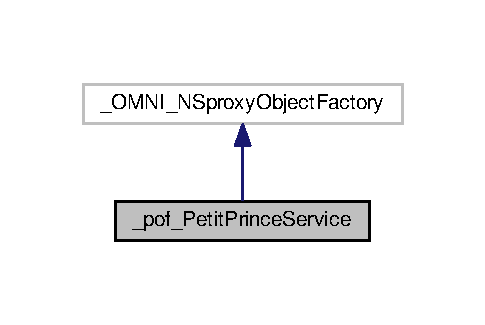
\includegraphics[width=233pt]{class__pof___petit_prince_service__inherit__graph}
\end{center}
\end{figure}


Collaboration diagram for \+\_\+pof\+\_\+\+Petit\+Prince\+Service\+:
\nopagebreak
\begin{figure}[H]
\begin{center}
\leavevmode
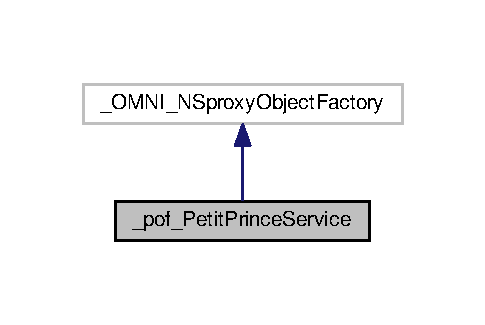
\includegraphics[width=233pt]{class__pof___petit_prince_service__coll__graph}
\end{center}
\end{figure}
\subsection*{Public Member Functions}
\begin{DoxyCompactItemize}
\item 
\hyperlink{class__pof___petit_prince_service_a7a0313a18bc00a15e942f157f91b71a4}{\+\_\+pof\+\_\+\+Petit\+Prince\+Service} ()
\item 
virtual \hyperlink{class__pof___petit_prince_service_a6b090844c1622edbfc710950015af98f}{$\sim$\+\_\+pof\+\_\+\+Petit\+Prince\+Service} ()
\item 
virtual omni\+Obj\+Ref $\ast$ \hyperlink{class__pof___petit_prince_service_a46038a17c269d931f5bef9478b358d1c}{new\+Obj\+Ref} (omni\+I\+OR $\ast$, omni\+Identity $\ast$)
\item 
virtual \+\_\+\+C\+O\+R\+B\+A\+\_\+\+Boolean \hyperlink{class__pof___petit_prince_service_a2600fc827ae27237fe960e3231ed9182}{is\+\_\+a} (const char $\ast$) const 
\end{DoxyCompactItemize}


\subsection{Constructor \& Destructor Documentation}
\index{\+\_\+pof\+\_\+\+Petit\+Prince\+Service@{\+\_\+pof\+\_\+\+Petit\+Prince\+Service}!\+\_\+pof\+\_\+\+Petit\+Prince\+Service@{\+\_\+pof\+\_\+\+Petit\+Prince\+Service}}
\index{\+\_\+pof\+\_\+\+Petit\+Prince\+Service@{\+\_\+pof\+\_\+\+Petit\+Prince\+Service}!\+\_\+pof\+\_\+\+Petit\+Prince\+Service@{\+\_\+pof\+\_\+\+Petit\+Prince\+Service}}
\subsubsection[{\texorpdfstring{\+\_\+pof\+\_\+\+Petit\+Prince\+Service()}{_pof_PetitPrinceService()}}]{\setlength{\rightskip}{0pt plus 5cm}\+\_\+pof\+\_\+\+Petit\+Prince\+Service\+::\+\_\+pof\+\_\+\+Petit\+Prince\+Service (
\begin{DoxyParamCaption}
{}
\end{DoxyParamCaption}
)\hspace{0.3cm}{\ttfamily [inline]}}\hypertarget{class__pof___petit_prince_service_a7a0313a18bc00a15e942f157f91b71a4}{}\label{class__pof___petit_prince_service_a7a0313a18bc00a15e942f157f91b71a4}
\index{\+\_\+pof\+\_\+\+Petit\+Prince\+Service@{\+\_\+pof\+\_\+\+Petit\+Prince\+Service}!````~\+\_\+pof\+\_\+\+Petit\+Prince\+Service@{$\sim$\+\_\+pof\+\_\+\+Petit\+Prince\+Service}}
\index{````~\+\_\+pof\+\_\+\+Petit\+Prince\+Service@{$\sim$\+\_\+pof\+\_\+\+Petit\+Prince\+Service}!\+\_\+pof\+\_\+\+Petit\+Prince\+Service@{\+\_\+pof\+\_\+\+Petit\+Prince\+Service}}
\subsubsection[{\texorpdfstring{$\sim$\+\_\+pof\+\_\+\+Petit\+Prince\+Service()}{~_pof_PetitPrinceService()}}]{\setlength{\rightskip}{0pt plus 5cm}virtual \+\_\+pof\+\_\+\+Petit\+Prince\+Service\+::$\sim$\+\_\+pof\+\_\+\+Petit\+Prince\+Service (
\begin{DoxyParamCaption}
{}
\end{DoxyParamCaption}
)\hspace{0.3cm}{\ttfamily [virtual]}}\hypertarget{class__pof___petit_prince_service_a6b090844c1622edbfc710950015af98f}{}\label{class__pof___petit_prince_service_a6b090844c1622edbfc710950015af98f}


\subsection{Member Function Documentation}
\index{\+\_\+pof\+\_\+\+Petit\+Prince\+Service@{\+\_\+pof\+\_\+\+Petit\+Prince\+Service}!is\+\_\+a@{is\+\_\+a}}
\index{is\+\_\+a@{is\+\_\+a}!\+\_\+pof\+\_\+\+Petit\+Prince\+Service@{\+\_\+pof\+\_\+\+Petit\+Prince\+Service}}
\subsubsection[{\texorpdfstring{is\+\_\+a(const char $\ast$) const }{is_a(const char *) const }}]{\setlength{\rightskip}{0pt plus 5cm}virtual \+\_\+\+C\+O\+R\+B\+A\+\_\+\+Boolean \+\_\+pof\+\_\+\+Petit\+Prince\+Service\+::is\+\_\+a (
\begin{DoxyParamCaption}
\item[{const char $\ast$}]{}
\end{DoxyParamCaption}
) const\hspace{0.3cm}{\ttfamily [virtual]}}\hypertarget{class__pof___petit_prince_service_a2600fc827ae27237fe960e3231ed9182}{}\label{class__pof___petit_prince_service_a2600fc827ae27237fe960e3231ed9182}
\index{\+\_\+pof\+\_\+\+Petit\+Prince\+Service@{\+\_\+pof\+\_\+\+Petit\+Prince\+Service}!new\+Obj\+Ref@{new\+Obj\+Ref}}
\index{new\+Obj\+Ref@{new\+Obj\+Ref}!\+\_\+pof\+\_\+\+Petit\+Prince\+Service@{\+\_\+pof\+\_\+\+Petit\+Prince\+Service}}
\subsubsection[{\texorpdfstring{new\+Obj\+Ref(omni\+I\+O\+R $\ast$, omni\+Identity $\ast$)}{newObjRef(omniIOR *, omniIdentity *)}}]{\setlength{\rightskip}{0pt plus 5cm}virtual omni\+Obj\+Ref$\ast$ \+\_\+pof\+\_\+\+Petit\+Prince\+Service\+::new\+Obj\+Ref (
\begin{DoxyParamCaption}
\item[{omni\+I\+OR $\ast$}]{, }
\item[{omni\+Identity $\ast$}]{}
\end{DoxyParamCaption}
)\hspace{0.3cm}{\ttfamily [virtual]}}\hypertarget{class__pof___petit_prince_service_a46038a17c269d931f5bef9478b358d1c}{}\label{class__pof___petit_prince_service_a46038a17c269d931f5bef9478b358d1c}


The documentation for this class was generated from the following file\+:\begin{DoxyCompactItemize}
\item 
hdr/\hyperlink{_petit_prince_8hpp}{Petit\+Prince.\+hpp}\end{DoxyCompactItemize}

\hypertarget{class_circle}{}\section{Circle Class Reference}
\label{class_circle}\index{Circle@{Circle}}


{\ttfamily \#include $<$Petit\+Prince.\+hpp$>$}



Inheritance diagram for Circle\+:
\nopagebreak
\begin{figure}[H]
\begin{center}
\leavevmode
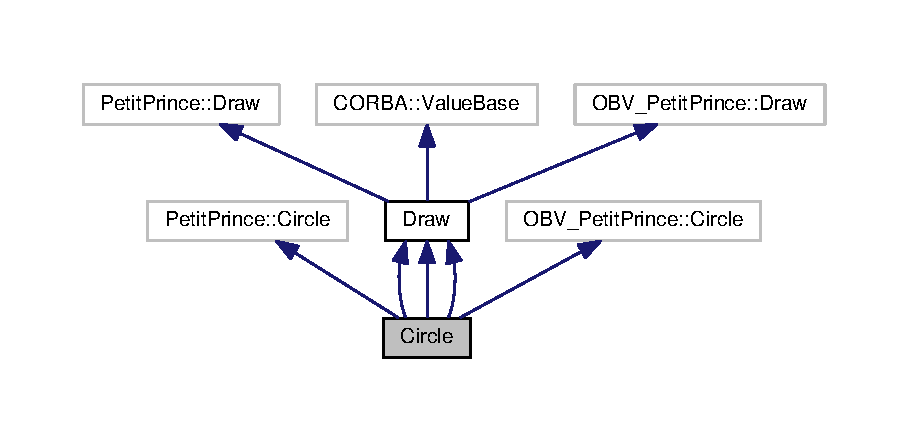
\includegraphics[width=326pt]{class_circle__inherit__graph}
\end{center}
\end{figure}


Collaboration diagram for Circle\+:
\nopagebreak
\begin{figure}[H]
\begin{center}
\leavevmode
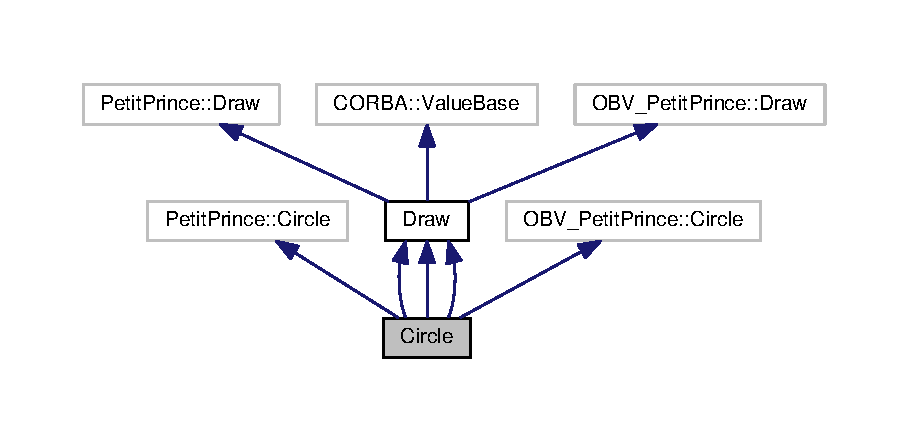
\includegraphics[width=326pt]{class_circle__coll__graph}
\end{center}
\end{figure}
\subsection*{Public Types}
\begin{DoxyCompactItemize}
\item 
typedef \hyperlink{class_circle}{Circle} $\ast$ \hyperlink{class_circle_ae284325f0ac7647d6e137e8a3f507f38}{\+\_\+ptr\+\_\+type}
\item 
typedef \hyperlink{_petit_prince_8hpp_ac2106cf1632c65be064ea3929f62047b}{Circle\+\_\+var} \hyperlink{class_circle_a193392939eca82b9195367ac5be1461a}{\+\_\+var\+\_\+type}
\end{DoxyCompactItemize}
\subsection*{Public Member Functions}
\begin{DoxyCompactItemize}
\item 
virtual \+::C\+O\+R\+B\+A\+::\+Value\+Base $\ast$ \hyperlink{class_circle_a77491043677d6e55c0647af478178bb3}{\+\_\+copy\+\_\+value} ()
\item 
virtual \hyperlink{struct_point}{Point} \hyperlink{class_circle_a7e6386f745d6255a2ddec2a53ff514b7}{center} ()=0
\item 
virtual void \hyperlink{class_circle_a9c4d4e9ec2a2e59f0c8d0c3f36e10edc}{center} (const \+::Petit\+Prince\+::\+Point \&\+\_\+v)=0
\item 
virtual \+::C\+O\+R\+B\+A\+::\+Double \hyperlink{class_circle_a1ddff289fde40dc6c25963c0c7b8d985}{ray} ()=0
\item 
virtual void \hyperlink{class_circle_a850aad5e97721700746efd3d82af1487}{ray} (\+::C\+O\+R\+B\+A\+::\+Double \+\_\+v)=0
\item 
virtual const char $\ast$ \hyperlink{class_circle_aef9e3dad8cb215413d3d9371c21312ba}{\+\_\+\+N\+P\+\_\+repository\+Id} () const 
\item 
virtual const char $\ast$ \hyperlink{class_circle_a2b46a87a83e6e4953bf3cbd507a99e26}{\+\_\+\+N\+P\+\_\+repository\+Id} (\+::C\+O\+R\+B\+A\+::\+U\+Long \&\+\_\+hashval) const 
\item 
virtual const \+\_\+omni\+\_\+\+Value\+Ids $\ast$ \hyperlink{class_circle_aaf148f2aa3a4bc47c990850800897ff9}{\+\_\+\+N\+P\+\_\+truncatable\+Ids} () const 
\item 
virtual \+::C\+O\+R\+B\+A\+::\+Boolean \hyperlink{class_circle_a5c0763ec17a208a2e25796b7714975cf}{\+\_\+\+N\+P\+\_\+custom} () const 
\item 
virtual void $\ast$ \hyperlink{class_circle_a4bcb25e2b518b4674bf81439c8f4ef6a}{\+\_\+ptr\+To\+Value} (const char $\ast$\hyperlink{class_draw_a50509da989141b00a5ae22d68a4d5856}{id})
\item 
virtual void \hyperlink{class_circle_af2d05d9a1c7ac75312e9e778b55a5625}{\+\_\+\+P\+R\+\_\+marshal\+\_\+state} (cdr\+Stream \&) const 
\item 
virtual void \hyperlink{class_circle_a7756078d5d749f39cd6620de130cfd0e}{\+\_\+\+P\+R\+\_\+unmarshal\+\_\+state} (cdr\+Stream \&)
\item 
virtual void \hyperlink{class_circle_a5a2cf4d7bb6f06052c34ecf0467cbe69}{\+\_\+\+P\+R\+\_\+copy\+\_\+state} (\hyperlink{class_circle}{Circle} $\ast$)
\end{DoxyCompactItemize}
\subsection*{Static Public Member Functions}
\begin{DoxyCompactItemize}
\item 
static \hyperlink{class_draw_a5164256572b3c4123ceecd1897c248dd}{\+\_\+ptr\+\_\+type} \hyperlink{class_circle_a264dbd97a8e3819388a008d722aab612}{\+\_\+downcast} (\+::C\+O\+R\+B\+A\+::\+Value\+Base $\ast$)
\item 
static void \hyperlink{class_circle_a6b682a01a8bf70dad668ec3f1fc1c5ef}{\+\_\+\+N\+P\+\_\+marshal} (\hyperlink{class_circle}{Circle} $\ast$, cdr\+Stream \&)
\item 
static \hyperlink{class_circle}{Circle} $\ast$ \hyperlink{class_circle_ae8e42637a424b531bcba7cb48fc398ef}{\+\_\+\+N\+P\+\_\+unmarshal} (cdr\+Stream \&)
\end{DoxyCompactItemize}
\subsection*{Static Public Attributes}
\begin{DoxyCompactItemize}
\item 
static \hyperlink{_petit_prince_8hpp_a5f7bf7cddb608c2aad7c95f55f8a33c5}{\+\_\+core\+\_\+attr} const char $\ast$ \hyperlink{class_circle_a3cc85c810268073e3c3f0519aa3b12a0}{\+\_\+\+P\+D\+\_\+repo\+Id}
\end{DoxyCompactItemize}
\subsection*{Protected Member Functions}
\begin{DoxyCompactItemize}
\item 
\hyperlink{class_circle_ad1ecfcfc7bf34529c6a6d6c448bf70fe}{Circle} ()
\item 
virtual \hyperlink{class_circle_ad02555ca63f3574193b958c49f81d178}{$\sim$\+Circle} ()
\item 
\hyperlink{class_circle_ad1ecfcfc7bf34529c6a6d6c448bf70fe}{Circle} ()
\item 
virtual \hyperlink{class_circle_ad02555ca63f3574193b958c49f81d178}{$\sim$\+Circle} ()
\end{DoxyCompactItemize}


\subsection{Member Typedef Documentation}
\index{Circle@{Circle}!\+\_\+ptr\+\_\+type@{\+\_\+ptr\+\_\+type}}
\index{\+\_\+ptr\+\_\+type@{\+\_\+ptr\+\_\+type}!Circle@{Circle}}
\subsubsection[{\texorpdfstring{\+\_\+ptr\+\_\+type}{_ptr_type}}]{\setlength{\rightskip}{0pt plus 5cm}typedef {\bf Circle}$\ast$ {\bf Circle\+::\+\_\+ptr\+\_\+type}}\hypertarget{class_circle_ae284325f0ac7647d6e137e8a3f507f38}{}\label{class_circle_ae284325f0ac7647d6e137e8a3f507f38}
\index{Circle@{Circle}!\+\_\+var\+\_\+type@{\+\_\+var\+\_\+type}}
\index{\+\_\+var\+\_\+type@{\+\_\+var\+\_\+type}!Circle@{Circle}}
\subsubsection[{\texorpdfstring{\+\_\+var\+\_\+type}{_var_type}}]{\setlength{\rightskip}{0pt plus 5cm}typedef {\bf Circle\+\_\+var} {\bf Circle\+::\+\_\+var\+\_\+type}}\hypertarget{class_circle_a193392939eca82b9195367ac5be1461a}{}\label{class_circle_a193392939eca82b9195367ac5be1461a}


\subsection{Constructor \& Destructor Documentation}
\index{Circle@{Circle}!Circle@{Circle}}
\index{Circle@{Circle}!Circle@{Circle}}
\subsubsection[{\texorpdfstring{Circle()}{Circle()}}]{\setlength{\rightskip}{0pt plus 5cm}Circle\+::\+Circle (
\begin{DoxyParamCaption}
{}
\end{DoxyParamCaption}
)\hspace{0.3cm}{\ttfamily [protected]}}\hypertarget{class_circle_ad1ecfcfc7bf34529c6a6d6c448bf70fe}{}\label{class_circle_ad1ecfcfc7bf34529c6a6d6c448bf70fe}
\index{Circle@{Circle}!````~Circle@{$\sim$\+Circle}}
\index{````~Circle@{$\sim$\+Circle}!Circle@{Circle}}
\subsubsection[{\texorpdfstring{$\sim$\+Circle()}{~Circle()}}]{\setlength{\rightskip}{0pt plus 5cm}virtual Circle\+::$\sim$\+Circle (
\begin{DoxyParamCaption}
{}
\end{DoxyParamCaption}
)\hspace{0.3cm}{\ttfamily [protected]}, {\ttfamily [virtual]}}\hypertarget{class_circle_ad02555ca63f3574193b958c49f81d178}{}\label{class_circle_ad02555ca63f3574193b958c49f81d178}
\index{Circle@{Circle}!Circle@{Circle}}
\index{Circle@{Circle}!Circle@{Circle}}
\subsubsection[{\texorpdfstring{Circle()}{Circle()}}]{\setlength{\rightskip}{0pt plus 5cm}Circle\+::\+Circle (
\begin{DoxyParamCaption}
{}
\end{DoxyParamCaption}
)\hspace{0.3cm}{\ttfamily [protected]}}\hypertarget{class_circle_ad1ecfcfc7bf34529c6a6d6c448bf70fe}{}\label{class_circle_ad1ecfcfc7bf34529c6a6d6c448bf70fe}
\index{Circle@{Circle}!````~Circle@{$\sim$\+Circle}}
\index{````~Circle@{$\sim$\+Circle}!Circle@{Circle}}
\subsubsection[{\texorpdfstring{$\sim$\+Circle()}{~Circle()}}]{\setlength{\rightskip}{0pt plus 5cm}virtual Circle\+::$\sim$\+Circle (
\begin{DoxyParamCaption}
{}
\end{DoxyParamCaption}
)\hspace{0.3cm}{\ttfamily [protected]}, {\ttfamily [virtual]}}\hypertarget{class_circle_ad02555ca63f3574193b958c49f81d178}{}\label{class_circle_ad02555ca63f3574193b958c49f81d178}


\subsection{Member Function Documentation}
\index{Circle@{Circle}!\+\_\+copy\+\_\+value@{\+\_\+copy\+\_\+value}}
\index{\+\_\+copy\+\_\+value@{\+\_\+copy\+\_\+value}!Circle@{Circle}}
\subsubsection[{\texorpdfstring{\+\_\+copy\+\_\+value()}{_copy_value()}}]{\setlength{\rightskip}{0pt plus 5cm}virtual \+::C\+O\+R\+B\+A\+::\+Value\+Base$\ast$ Circle\+::\+\_\+copy\+\_\+value (
\begin{DoxyParamCaption}
{}
\end{DoxyParamCaption}
)}\hypertarget{class_circle_a77491043677d6e55c0647af478178bb3}{}\label{class_circle_a77491043677d6e55c0647af478178bb3}
\index{Circle@{Circle}!\+\_\+downcast@{\+\_\+downcast}}
\index{\+\_\+downcast@{\+\_\+downcast}!Circle@{Circle}}
\subsubsection[{\texorpdfstring{\+\_\+downcast(\+::\+C\+O\+R\+B\+A\+::\+Value\+Base $\ast$)}{_downcast(::CORBA::ValueBase *)}}]{\setlength{\rightskip}{0pt plus 5cm}static {\bf \+\_\+ptr\+\_\+type} Circle\+::\+\_\+downcast (
\begin{DoxyParamCaption}
\item[{\+::C\+O\+R\+B\+A\+::\+Value\+Base $\ast$}]{}
\end{DoxyParamCaption}
)\hspace{0.3cm}{\ttfamily [static]}}\hypertarget{class_circle_a264dbd97a8e3819388a008d722aab612}{}\label{class_circle_a264dbd97a8e3819388a008d722aab612}
\index{Circle@{Circle}!\+\_\+\+N\+P\+\_\+custom@{\+\_\+\+N\+P\+\_\+custom}}
\index{\+\_\+\+N\+P\+\_\+custom@{\+\_\+\+N\+P\+\_\+custom}!Circle@{Circle}}
\subsubsection[{\texorpdfstring{\+\_\+\+N\+P\+\_\+custom() const }{_NP_custom() const }}]{\setlength{\rightskip}{0pt plus 5cm}virtual \+::C\+O\+R\+B\+A\+::\+Boolean Circle\+::\+\_\+\+N\+P\+\_\+custom (
\begin{DoxyParamCaption}
{}
\end{DoxyParamCaption}
) const}\hypertarget{class_circle_a5c0763ec17a208a2e25796b7714975cf}{}\label{class_circle_a5c0763ec17a208a2e25796b7714975cf}
\index{Circle@{Circle}!\+\_\+\+N\+P\+\_\+marshal@{\+\_\+\+N\+P\+\_\+marshal}}
\index{\+\_\+\+N\+P\+\_\+marshal@{\+\_\+\+N\+P\+\_\+marshal}!Circle@{Circle}}
\subsubsection[{\texorpdfstring{\+\_\+\+N\+P\+\_\+marshal(\+Circle $\ast$, cdr\+Stream \&)}{_NP_marshal(Circle *, cdrStream &)}}]{\setlength{\rightskip}{0pt plus 5cm}static void Circle\+::\+\_\+\+N\+P\+\_\+marshal (
\begin{DoxyParamCaption}
\item[{{\bf Circle} $\ast$}]{, }
\item[{cdr\+Stream \&}]{}
\end{DoxyParamCaption}
)\hspace{0.3cm}{\ttfamily [static]}}\hypertarget{class_circle_a6b682a01a8bf70dad668ec3f1fc1c5ef}{}\label{class_circle_a6b682a01a8bf70dad668ec3f1fc1c5ef}
\index{Circle@{Circle}!\+\_\+\+N\+P\+\_\+repository\+Id@{\+\_\+\+N\+P\+\_\+repository\+Id}}
\index{\+\_\+\+N\+P\+\_\+repository\+Id@{\+\_\+\+N\+P\+\_\+repository\+Id}!Circle@{Circle}}
\subsubsection[{\texorpdfstring{\+\_\+\+N\+P\+\_\+repository\+Id() const }{_NP_repositoryId() const }}]{\setlength{\rightskip}{0pt plus 5cm}virtual const char$\ast$ Circle\+::\+\_\+\+N\+P\+\_\+repository\+Id (
\begin{DoxyParamCaption}
{}
\end{DoxyParamCaption}
) const\hspace{0.3cm}{\ttfamily [virtual]}}\hypertarget{class_circle_aef9e3dad8cb215413d3d9371c21312ba}{}\label{class_circle_aef9e3dad8cb215413d3d9371c21312ba}


Reimplemented from \hyperlink{class_draw_a90d2c0a9b6aed68ca30ea2a7187317dc}{Draw}.

\index{Circle@{Circle}!\+\_\+\+N\+P\+\_\+repository\+Id@{\+\_\+\+N\+P\+\_\+repository\+Id}}
\index{\+\_\+\+N\+P\+\_\+repository\+Id@{\+\_\+\+N\+P\+\_\+repository\+Id}!Circle@{Circle}}
\subsubsection[{\texorpdfstring{\+\_\+\+N\+P\+\_\+repository\+Id(\+::\+C\+O\+R\+B\+A\+::\+U\+Long \&\+\_\+hashval) const }{_NP_repositoryId(::CORBA::ULong &_hashval) const }}]{\setlength{\rightskip}{0pt plus 5cm}virtual const char$\ast$ Circle\+::\+\_\+\+N\+P\+\_\+repository\+Id (
\begin{DoxyParamCaption}
\item[{\+::C\+O\+R\+B\+A\+::\+U\+Long \&}]{\+\_\+hashval}
\end{DoxyParamCaption}
) const\hspace{0.3cm}{\ttfamily [virtual]}}\hypertarget{class_circle_a2b46a87a83e6e4953bf3cbd507a99e26}{}\label{class_circle_a2b46a87a83e6e4953bf3cbd507a99e26}


Reimplemented from \hyperlink{class_draw_ae24df04b0f119c2fb6fd525a041f081d}{Draw}.

\index{Circle@{Circle}!\+\_\+\+N\+P\+\_\+truncatable\+Ids@{\+\_\+\+N\+P\+\_\+truncatable\+Ids}}
\index{\+\_\+\+N\+P\+\_\+truncatable\+Ids@{\+\_\+\+N\+P\+\_\+truncatable\+Ids}!Circle@{Circle}}
\subsubsection[{\texorpdfstring{\+\_\+\+N\+P\+\_\+truncatable\+Ids() const }{_NP_truncatableIds() const }}]{\setlength{\rightskip}{0pt plus 5cm}virtual const \+\_\+omni\+\_\+\+Value\+Ids$\ast$ Circle\+::\+\_\+\+N\+P\+\_\+truncatable\+Ids (
\begin{DoxyParamCaption}
{}
\end{DoxyParamCaption}
) const\hspace{0.3cm}{\ttfamily [virtual]}}\hypertarget{class_circle_aaf148f2aa3a4bc47c990850800897ff9}{}\label{class_circle_aaf148f2aa3a4bc47c990850800897ff9}


Reimplemented from \hyperlink{class_draw_a10a319bcb2ef5d6ac5439859fe9f126e}{Draw}.

\index{Circle@{Circle}!\+\_\+\+N\+P\+\_\+unmarshal@{\+\_\+\+N\+P\+\_\+unmarshal}}
\index{\+\_\+\+N\+P\+\_\+unmarshal@{\+\_\+\+N\+P\+\_\+unmarshal}!Circle@{Circle}}
\subsubsection[{\texorpdfstring{\+\_\+\+N\+P\+\_\+unmarshal(cdr\+Stream \&)}{_NP_unmarshal(cdrStream &)}}]{\setlength{\rightskip}{0pt plus 5cm}static {\bf Circle}$\ast$ Circle\+::\+\_\+\+N\+P\+\_\+unmarshal (
\begin{DoxyParamCaption}
\item[{cdr\+Stream \&}]{}
\end{DoxyParamCaption}
)\hspace{0.3cm}{\ttfamily [static]}}\hypertarget{class_circle_ae8e42637a424b531bcba7cb48fc398ef}{}\label{class_circle_ae8e42637a424b531bcba7cb48fc398ef}
\index{Circle@{Circle}!\+\_\+\+P\+R\+\_\+copy\+\_\+state@{\+\_\+\+P\+R\+\_\+copy\+\_\+state}}
\index{\+\_\+\+P\+R\+\_\+copy\+\_\+state@{\+\_\+\+P\+R\+\_\+copy\+\_\+state}!Circle@{Circle}}
\subsubsection[{\texorpdfstring{\+\_\+\+P\+R\+\_\+copy\+\_\+state(\+Circle $\ast$)}{_PR_copy_state(Circle *)}}]{\setlength{\rightskip}{0pt plus 5cm}virtual void Circle\+::\+\_\+\+P\+R\+\_\+copy\+\_\+state (
\begin{DoxyParamCaption}
\item[{{\bf Circle} $\ast$}]{}
\end{DoxyParamCaption}
)\hspace{0.3cm}{\ttfamily [virtual]}}\hypertarget{class_circle_a5a2cf4d7bb6f06052c34ecf0467cbe69}{}\label{class_circle_a5a2cf4d7bb6f06052c34ecf0467cbe69}
\index{Circle@{Circle}!\+\_\+\+P\+R\+\_\+marshal\+\_\+state@{\+\_\+\+P\+R\+\_\+marshal\+\_\+state}}
\index{\+\_\+\+P\+R\+\_\+marshal\+\_\+state@{\+\_\+\+P\+R\+\_\+marshal\+\_\+state}!Circle@{Circle}}
\subsubsection[{\texorpdfstring{\+\_\+\+P\+R\+\_\+marshal\+\_\+state(cdr\+Stream \&) const }{_PR_marshal_state(cdrStream &) const }}]{\setlength{\rightskip}{0pt plus 5cm}virtual void Circle\+::\+\_\+\+P\+R\+\_\+marshal\+\_\+state (
\begin{DoxyParamCaption}
\item[{cdr\+Stream \&}]{}
\end{DoxyParamCaption}
) const\hspace{0.3cm}{\ttfamily [virtual]}}\hypertarget{class_circle_af2d05d9a1c7ac75312e9e778b55a5625}{}\label{class_circle_af2d05d9a1c7ac75312e9e778b55a5625}


Reimplemented from \hyperlink{class_draw_adfa1e0ac94bad822e332caeddc17f02a}{Draw}.

\index{Circle@{Circle}!\+\_\+\+P\+R\+\_\+unmarshal\+\_\+state@{\+\_\+\+P\+R\+\_\+unmarshal\+\_\+state}}
\index{\+\_\+\+P\+R\+\_\+unmarshal\+\_\+state@{\+\_\+\+P\+R\+\_\+unmarshal\+\_\+state}!Circle@{Circle}}
\subsubsection[{\texorpdfstring{\+\_\+\+P\+R\+\_\+unmarshal\+\_\+state(cdr\+Stream \&)}{_PR_unmarshal_state(cdrStream &)}}]{\setlength{\rightskip}{0pt plus 5cm}virtual void Circle\+::\+\_\+\+P\+R\+\_\+unmarshal\+\_\+state (
\begin{DoxyParamCaption}
\item[{cdr\+Stream \&}]{}
\end{DoxyParamCaption}
)\hspace{0.3cm}{\ttfamily [virtual]}}\hypertarget{class_circle_a7756078d5d749f39cd6620de130cfd0e}{}\label{class_circle_a7756078d5d749f39cd6620de130cfd0e}


Reimplemented from \hyperlink{class_draw_a62dc59ec12f9ebd4da1f3448dbec683f}{Draw}.

\index{Circle@{Circle}!\+\_\+ptr\+To\+Value@{\+\_\+ptr\+To\+Value}}
\index{\+\_\+ptr\+To\+Value@{\+\_\+ptr\+To\+Value}!Circle@{Circle}}
\subsubsection[{\texorpdfstring{\+\_\+ptr\+To\+Value(const char $\ast$id)}{_ptrToValue(const char *id)}}]{\setlength{\rightskip}{0pt plus 5cm}virtual void$\ast$ Circle\+::\+\_\+ptr\+To\+Value (
\begin{DoxyParamCaption}
\item[{const char $\ast$}]{id}
\end{DoxyParamCaption}
)\hspace{0.3cm}{\ttfamily [virtual]}}\hypertarget{class_circle_a4bcb25e2b518b4674bf81439c8f4ef6a}{}\label{class_circle_a4bcb25e2b518b4674bf81439c8f4ef6a}


Reimplemented from \hyperlink{class_draw_a2924173c6238dd077531f555324155b9}{Draw}.

\index{Circle@{Circle}!center@{center}}
\index{center@{center}!Circle@{Circle}}
\subsubsection[{\texorpdfstring{center()=0}{center()=0}}]{\setlength{\rightskip}{0pt plus 5cm}virtual {\bf Point} Circle\+::center (
\begin{DoxyParamCaption}
{}
\end{DoxyParamCaption}
)\hspace{0.3cm}{\ttfamily [pure virtual]}}\hypertarget{class_circle_a7e6386f745d6255a2ddec2a53ff514b7}{}\label{class_circle_a7e6386f745d6255a2ddec2a53ff514b7}
\index{Circle@{Circle}!center@{center}}
\index{center@{center}!Circle@{Circle}}
\subsubsection[{\texorpdfstring{center(const \+::\+Petit\+Prince\+::\+Point \&\+\_\+v)=0}{center(const ::PetitPrince::Point &_v)=0}}]{\setlength{\rightskip}{0pt plus 5cm}virtual void Circle\+::center (
\begin{DoxyParamCaption}
\item[{const \+::Petit\+Prince\+::\+Point \&}]{\+\_\+v}
\end{DoxyParamCaption}
)\hspace{0.3cm}{\ttfamily [pure virtual]}}\hypertarget{class_circle_a9c4d4e9ec2a2e59f0c8d0c3f36e10edc}{}\label{class_circle_a9c4d4e9ec2a2e59f0c8d0c3f36e10edc}
\index{Circle@{Circle}!ray@{ray}}
\index{ray@{ray}!Circle@{Circle}}
\subsubsection[{\texorpdfstring{ray()=0}{ray()=0}}]{\setlength{\rightskip}{0pt plus 5cm}virtual \+::C\+O\+R\+B\+A\+::\+Double Circle\+::ray (
\begin{DoxyParamCaption}
{}
\end{DoxyParamCaption}
)\hspace{0.3cm}{\ttfamily [pure virtual]}}\hypertarget{class_circle_a1ddff289fde40dc6c25963c0c7b8d985}{}\label{class_circle_a1ddff289fde40dc6c25963c0c7b8d985}
\index{Circle@{Circle}!ray@{ray}}
\index{ray@{ray}!Circle@{Circle}}
\subsubsection[{\texorpdfstring{ray(\+::\+C\+O\+R\+B\+A\+::\+Double \+\_\+v)=0}{ray(::CORBA::Double _v)=0}}]{\setlength{\rightskip}{0pt plus 5cm}virtual void Circle\+::ray (
\begin{DoxyParamCaption}
\item[{\+::C\+O\+R\+B\+A\+::\+Double}]{\+\_\+v}
\end{DoxyParamCaption}
)\hspace{0.3cm}{\ttfamily [pure virtual]}}\hypertarget{class_circle_a850aad5e97721700746efd3d82af1487}{}\label{class_circle_a850aad5e97721700746efd3d82af1487}


\subsection{Member Data Documentation}
\index{Circle@{Circle}!\+\_\+\+P\+D\+\_\+repo\+Id@{\+\_\+\+P\+D\+\_\+repo\+Id}}
\index{\+\_\+\+P\+D\+\_\+repo\+Id@{\+\_\+\+P\+D\+\_\+repo\+Id}!Circle@{Circle}}
\subsubsection[{\texorpdfstring{\+\_\+\+P\+D\+\_\+repo\+Id}{_PD_repoId}}]{\setlength{\rightskip}{0pt plus 5cm}{\bf \+\_\+core\+\_\+attr} const char$\ast$ Circle\+::\+\_\+\+P\+D\+\_\+repo\+Id\hspace{0.3cm}{\ttfamily [static]}}\hypertarget{class_circle_a3cc85c810268073e3c3f0519aa3b12a0}{}\label{class_circle_a3cc85c810268073e3c3f0519aa3b12a0}


The documentation for this class was generated from the following file\+:\begin{DoxyCompactItemize}
\item 
hdr/\hyperlink{_petit_prince_8hpp}{Petit\+Prince.\+hpp}\end{DoxyCompactItemize}

\hypertarget{class_circle___helper}{}\section{Circle\+\_\+\+Helper Class Reference}
\label{class_circle___helper}\index{Circle\+\_\+\+Helper@{Circle\+\_\+\+Helper}}


{\ttfamily \#include $<$Petit\+Prince.\+hpp$>$}

\subsection*{Static Public Member Functions}
\begin{DoxyCompactItemize}
\item 
static void \hyperlink{class_circle___helper_a115e4084464261621557ca250eaa9e79}{add\+\_\+ref} (\hyperlink{class_circle}{Circle} $\ast$)
\item 
static void \hyperlink{class_circle___helper_abcb622a266ec9c8397de32df927751c2}{remove\+\_\+ref} (\hyperlink{class_circle}{Circle} $\ast$)
\item 
static void \hyperlink{class_circle___helper_a088f6698df5e26bf79f0002e05d224f8}{marshal} (\hyperlink{class_circle}{Circle} $\ast$, cdr\+Stream \&)
\item 
static \hyperlink{class_circle}{Circle} $\ast$ \hyperlink{class_circle___helper_ad4bbb204d7ff7e587e03ce65c14bbee5}{unmarshal} (cdr\+Stream \&)
\end{DoxyCompactItemize}


\subsection{Member Function Documentation}
\index{Circle\+\_\+\+Helper@{Circle\+\_\+\+Helper}!add\+\_\+ref@{add\+\_\+ref}}
\index{add\+\_\+ref@{add\+\_\+ref}!Circle\+\_\+\+Helper@{Circle\+\_\+\+Helper}}
\subsubsection[{\texorpdfstring{add\+\_\+ref(\+Circle $\ast$)}{add_ref(Circle *)}}]{\setlength{\rightskip}{0pt plus 5cm}static void Circle\+\_\+\+Helper\+::add\+\_\+ref (
\begin{DoxyParamCaption}
\item[{{\bf Circle} $\ast$}]{}
\end{DoxyParamCaption}
)\hspace{0.3cm}{\ttfamily [static]}}\hypertarget{class_circle___helper_a115e4084464261621557ca250eaa9e79}{}\label{class_circle___helper_a115e4084464261621557ca250eaa9e79}
\index{Circle\+\_\+\+Helper@{Circle\+\_\+\+Helper}!marshal@{marshal}}
\index{marshal@{marshal}!Circle\+\_\+\+Helper@{Circle\+\_\+\+Helper}}
\subsubsection[{\texorpdfstring{marshal(\+Circle $\ast$, cdr\+Stream \&)}{marshal(Circle *, cdrStream &)}}]{\setlength{\rightskip}{0pt plus 5cm}static void Circle\+\_\+\+Helper\+::marshal (
\begin{DoxyParamCaption}
\item[{{\bf Circle} $\ast$}]{, }
\item[{cdr\+Stream \&}]{}
\end{DoxyParamCaption}
)\hspace{0.3cm}{\ttfamily [static]}}\hypertarget{class_circle___helper_a088f6698df5e26bf79f0002e05d224f8}{}\label{class_circle___helper_a088f6698df5e26bf79f0002e05d224f8}
\index{Circle\+\_\+\+Helper@{Circle\+\_\+\+Helper}!remove\+\_\+ref@{remove\+\_\+ref}}
\index{remove\+\_\+ref@{remove\+\_\+ref}!Circle\+\_\+\+Helper@{Circle\+\_\+\+Helper}}
\subsubsection[{\texorpdfstring{remove\+\_\+ref(\+Circle $\ast$)}{remove_ref(Circle *)}}]{\setlength{\rightskip}{0pt plus 5cm}static void Circle\+\_\+\+Helper\+::remove\+\_\+ref (
\begin{DoxyParamCaption}
\item[{{\bf Circle} $\ast$}]{}
\end{DoxyParamCaption}
)\hspace{0.3cm}{\ttfamily [static]}}\hypertarget{class_circle___helper_abcb622a266ec9c8397de32df927751c2}{}\label{class_circle___helper_abcb622a266ec9c8397de32df927751c2}
\index{Circle\+\_\+\+Helper@{Circle\+\_\+\+Helper}!unmarshal@{unmarshal}}
\index{unmarshal@{unmarshal}!Circle\+\_\+\+Helper@{Circle\+\_\+\+Helper}}
\subsubsection[{\texorpdfstring{unmarshal(cdr\+Stream \&)}{unmarshal(cdrStream &)}}]{\setlength{\rightskip}{0pt plus 5cm}static {\bf Circle}$\ast$ Circle\+\_\+\+Helper\+::unmarshal (
\begin{DoxyParamCaption}
\item[{cdr\+Stream \&}]{}
\end{DoxyParamCaption}
)\hspace{0.3cm}{\ttfamily [static]}}\hypertarget{class_circle___helper_ad4bbb204d7ff7e587e03ce65c14bbee5}{}\label{class_circle___helper_ad4bbb204d7ff7e587e03ce65c14bbee5}


The documentation for this class was generated from the following file\+:\begin{DoxyCompactItemize}
\item 
hdr/\hyperlink{_petit_prince_8hpp}{Petit\+Prince.\+hpp}\end{DoxyCompactItemize}

\hypertarget{class_draw}{}\section{Draw Class Reference}
\label{class_draw}\index{Draw@{Draw}}


This class is a virtual class that define the first behavior of each draws that will be implemented.  




{\ttfamily \#include $<$O\+B\+V\+\_\+\+Draw.\+hpp$>$}



Inheritance diagram for Draw\+:
\nopagebreak
\begin{figure}[H]
\begin{center}
\leavevmode
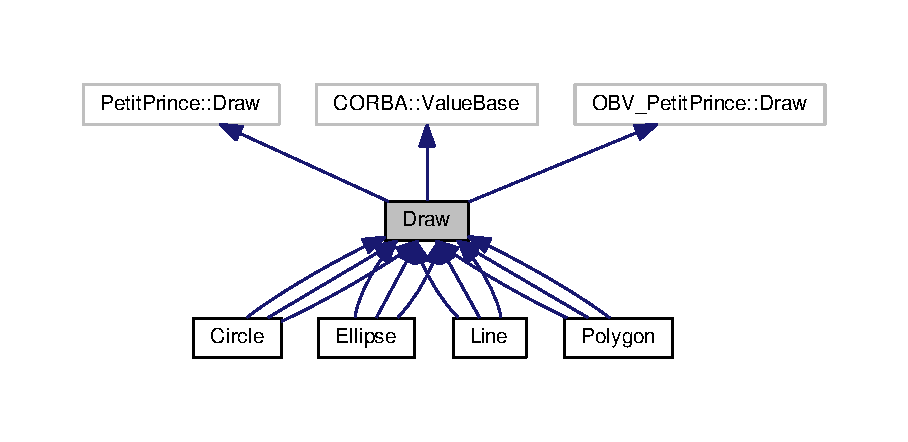
\includegraphics[width=350pt]{class_draw__inherit__graph}
\end{center}
\end{figure}


Collaboration diagram for Draw\+:
\nopagebreak
\begin{figure}[H]
\begin{center}
\leavevmode
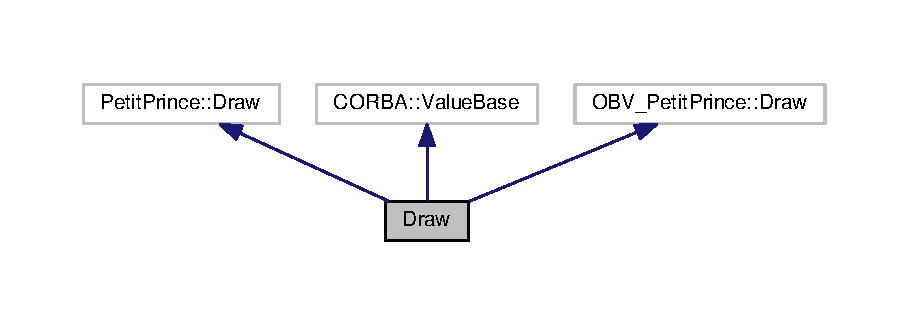
\includegraphics[width=350pt]{class_draw__coll__graph}
\end{center}
\end{figure}
\subsection*{Public Types}
\begin{DoxyCompactItemize}
\item 
typedef \hyperlink{class_draw}{Draw} $\ast$ \hyperlink{class_draw_a5164256572b3c4123ceecd1897c248dd}{\+\_\+ptr\+\_\+type}
\item 
typedef \hyperlink{_petit_prince_8hpp_ad6329853fd4733d5723ae5cc6c8a9f43}{Draw\+\_\+var} \hyperlink{class_draw_a0ef4fbc763491a2013fa08badb5ee934}{\+\_\+var\+\_\+type}
\end{DoxyCompactItemize}
\subsection*{Public Member Functions}
\begin{DoxyCompactItemize}
\item 
\+::C\+O\+R\+B\+A\+::\+Long \hyperlink{class_draw_a1bf27c5a59da9002d55936c947dce2cc}{id} () override
\item 
char $\ast$ \hyperlink{class_draw_a4781c654db63e069c8c5be017f6ccc34}{author} () override
\item 
\+::Petit\+Prince\+::\+Draw\+Seq $\ast$ \hyperlink{class_draw_ab51be1cb17bd03a3c8aba343e3d45013}{inner\+\_\+draws} () override
\item 
void \hyperlink{class_draw_a7ff3025eb06561c0c16ffbe2745b2315}{inner\+\_\+draws} (const \+::Petit\+Prince\+::\+Draw\+Seq \&\+\_\+v) override
\item 
\+::C\+O\+R\+B\+A\+::\+Double \hyperlink{class_draw_aeee0f92e6a2835212a7f3e44e4e41227}{mark} () override
\item 
void \hyperlink{class_draw_ac7ea79d2a2efff6c6b3ce9efeaf67a45}{mark} (\+::C\+O\+R\+B\+A\+::\+Double \+\_\+v) override
\item 
char $\ast$ \hyperlink{class_draw_a997583b775c33f224af795ab367cc400}{to\+String} () override
\item 
void \hyperlink{class_draw_a16806f06fc905a991a57921f20f7601f}{\+\_\+add\+\_\+ref} () override
\item 
\+::C\+O\+R\+B\+A\+::\+U\+Long \hyperlink{class_draw_ad420e80c785e510210fc7b8f3765d366}{\+\_\+refcount\+\_\+value} () override
\item 
void \hyperlink{class_draw_a7d465e9c8109a47928acf9d4b8f3204c}{\+\_\+remove\+\_\+ref} () override
\item 
virtual \+::C\+O\+R\+B\+A\+::\+Value\+Base $\ast$ \hyperlink{class_draw_a833b3c7cd298f64e57e2d91644c1fba0}{\+\_\+copy\+\_\+value} ()
\item 
virtual \+::C\+O\+R\+B\+A\+::\+Long \hyperlink{class_draw_a50509da989141b00a5ae22d68a4d5856}{id} ()=0
\item 
virtual char $\ast$ \hyperlink{class_draw_a4a1145eee8c06df2d81c99ad3ed40237}{author} ()=0
\item 
virtual \hyperlink{class_draw_seq}{Draw\+Seq} $\ast$ \hyperlink{class_draw_a8dfc05b32e3879efeb3b497abed032e8}{inner\+\_\+draws} ()=0
\item 
virtual void \hyperlink{class_draw_ae1c94fbdfc84aed1996ef1cdb9495076}{inner\+\_\+draws} (const \+::Petit\+Prince\+::\+Draw\+Seq \&\+\_\+v)=0
\item 
virtual \+::C\+O\+R\+B\+A\+::\+Double \hyperlink{class_draw_a24995593a9bf2ae75e2bfd9360064fa8}{mark} ()=0
\item 
virtual void \hyperlink{class_draw_aa4e3152cacbeda31c43d1fab6f54f4f2}{mark} (\+::C\+O\+R\+B\+A\+::\+Double \+\_\+v)=0
\item 
virtual \+::C\+O\+R\+B\+A\+::\+Double \hyperlink{class_draw_a0fb84e185ec13237aa456962d1eb0816}{area} ()=0
\item 
virtual \+::C\+O\+R\+B\+A\+::\+Double \hyperlink{class_draw_a7171f2b64135c81a41cb5a7a9926af52}{perimeter} ()=0
\item 
virtual void \hyperlink{class_draw_a39387bf248da4d7d91bee9099d4b6fca}{homothetie} (\+::C\+O\+R\+B\+A\+::\+Double indice)=0
\item 
virtual void \hyperlink{class_draw_a71e63b40c9505098652a94e06872fdc6}{translation} (\+::C\+O\+R\+B\+A\+::\+Double x,\+::C\+O\+R\+B\+A\+::\+Double y)=0
\item 
virtual void \hyperlink{class_draw_ab45c311ee0963a1a5e3ba3ac461e467c}{rotation} (\+::C\+O\+R\+B\+A\+::\+Double angle)=0
\item 
virtual void \hyperlink{class_draw_a1a10bbbeb1ccd4b10b04226f3fe10755}{sym\+Center} ()=0
\item 
virtual void \hyperlink{class_draw_aede358197311244da0fe937fb7e9573e}{sym\+Axial} ()=0
\item 
virtual char $\ast$ \hyperlink{class_draw_a0dd9c8b5127149b28e54bd602c797cca}{to\+String} ()=0
\item 
virtual const char $\ast$ \hyperlink{class_draw_a90d2c0a9b6aed68ca30ea2a7187317dc}{\+\_\+\+N\+P\+\_\+repository\+Id} () const 
\item 
virtual const char $\ast$ \hyperlink{class_draw_ae24df04b0f119c2fb6fd525a041f081d}{\+\_\+\+N\+P\+\_\+repository\+Id} (\+::C\+O\+R\+B\+A\+::\+U\+Long \&\+\_\+hashval) const 
\item 
virtual const \+\_\+omni\+\_\+\+Value\+Ids $\ast$ \hyperlink{class_draw_a10a319bcb2ef5d6ac5439859fe9f126e}{\+\_\+\+N\+P\+\_\+truncatable\+Ids} () const 
\item 
virtual \+::C\+O\+R\+B\+A\+::\+Boolean \hyperlink{class_draw_aab5e3083274138f65200f2516df70510}{\+\_\+\+N\+P\+\_\+custom} () const 
\item 
virtual void $\ast$ \hyperlink{class_draw_a2924173c6238dd077531f555324155b9}{\+\_\+ptr\+To\+Value} (const char $\ast$\hyperlink{class_draw_a1bf27c5a59da9002d55936c947dce2cc}{id})
\item 
virtual void \hyperlink{class_draw_adfa1e0ac94bad822e332caeddc17f02a}{\+\_\+\+P\+R\+\_\+marshal\+\_\+state} (cdr\+Stream \&) const 
\item 
virtual void \hyperlink{class_draw_a62dc59ec12f9ebd4da1f3448dbec683f}{\+\_\+\+P\+R\+\_\+unmarshal\+\_\+state} (cdr\+Stream \&)
\item 
virtual void \hyperlink{class_draw_a5832713920beeb0d47ef83caf919f185}{\+\_\+\+P\+R\+\_\+copy\+\_\+state} (\hyperlink{class_draw}{Draw} $\ast$)
\end{DoxyCompactItemize}
\subsection*{Static Public Member Functions}
\begin{DoxyCompactItemize}
\item 
static \hyperlink{class_draw_a5164256572b3c4123ceecd1897c248dd}{\+\_\+ptr\+\_\+type} \hyperlink{class_draw_adf5095556588059f6a3c1663e84e46c0}{\+\_\+downcast} (\+::C\+O\+R\+B\+A\+::\+Value\+Base $\ast$)
\item 
static void \hyperlink{class_draw_aa95f9c6dc4ba6f6d3477fc6432180594}{\+\_\+\+N\+P\+\_\+marshal} (\hyperlink{class_draw}{Draw} $\ast$, cdr\+Stream \&)
\item 
static \hyperlink{class_draw}{Draw} $\ast$ \hyperlink{class_draw_a3c3a65725a77c521aca9582928f5b298}{\+\_\+\+N\+P\+\_\+unmarshal} (cdr\+Stream \&)
\end{DoxyCompactItemize}
\subsection*{Static Public Attributes}
\begin{DoxyCompactItemize}
\item 
static \hyperlink{_petit_prince_8hpp_a5f7bf7cddb608c2aad7c95f55f8a33c5}{\+\_\+core\+\_\+attr} const char $\ast$ \hyperlink{class_draw_aa81c5a904a215524ca32f588126783bc}{\+\_\+\+P\+D\+\_\+repo\+Id}
\end{DoxyCompactItemize}
\subsection*{Protected Member Functions}
\begin{DoxyCompactItemize}
\item 
\hyperlink{class_draw_ad7d5df539676d880a1190ce78251b035}{Draw} (\+::C\+O\+R\+B\+A\+::\+Long \hyperlink{class_draw_a1bf27c5a59da9002d55936c947dce2cc}{id}, char $\ast$\hyperlink{class_draw_a4781c654db63e069c8c5be017f6ccc34}{author},\+::C\+O\+R\+B\+A\+::\+Double \hyperlink{class_draw_aeee0f92e6a2835212a7f3e44e4e41227}{mark})
\begin{DoxyCompactList}\small\item\em The protected constructor of the class \hyperlink{class_draw}{Draw}. Only called by sub classes. \end{DoxyCompactList}\item 
virtual \hyperlink{class_draw_a9c2feb77460265c202c60772ae05656a}{$\sim$\+Draw} ()
\item 
\hyperlink{class_draw_a7c808e2194e8659b401584773e26730e}{Draw} ()
\item 
virtual \hyperlink{class_draw_a9c2feb77460265c202c60772ae05656a}{$\sim$\+Draw} ()
\item 
\hyperlink{class_draw_a7c808e2194e8659b401584773e26730e}{Draw} ()
\item 
virtual \hyperlink{class_draw_a9c2feb77460265c202c60772ae05656a}{$\sim$\+Draw} ()
\end{DoxyCompactItemize}


\subsection{Detailed Description}
This class is a virtual class that define the first behavior of each draws that will be implemented. 

Definition at line 26 of file O\+B\+V\+\_\+\+Draw.\+hpp.



\subsection{Member Typedef Documentation}
\index{Draw@{Draw}!\+\_\+ptr\+\_\+type@{\+\_\+ptr\+\_\+type}}
\index{\+\_\+ptr\+\_\+type@{\+\_\+ptr\+\_\+type}!Draw@{Draw}}
\subsubsection[{\texorpdfstring{\+\_\+ptr\+\_\+type}{_ptr_type}}]{\setlength{\rightskip}{0pt plus 5cm}typedef {\bf Draw}$\ast$ {\bf Draw\+::\+\_\+ptr\+\_\+type}}\hypertarget{class_draw_a5164256572b3c4123ceecd1897c248dd}{}\label{class_draw_a5164256572b3c4123ceecd1897c248dd}


Definition at line 346 of file Petit\+Prince.\+hpp.

\index{Draw@{Draw}!\+\_\+var\+\_\+type@{\+\_\+var\+\_\+type}}
\index{\+\_\+var\+\_\+type@{\+\_\+var\+\_\+type}!Draw@{Draw}}
\subsubsection[{\texorpdfstring{\+\_\+var\+\_\+type}{_var_type}}]{\setlength{\rightskip}{0pt plus 5cm}typedef {\bf Draw\+\_\+var} {\bf Draw\+::\+\_\+var\+\_\+type}}\hypertarget{class_draw_a0ef4fbc763491a2013fa08badb5ee934}{}\label{class_draw_a0ef4fbc763491a2013fa08badb5ee934}


Definition at line 347 of file Petit\+Prince.\+hpp.



\subsection{Constructor \& Destructor Documentation}
\index{Draw@{Draw}!Draw@{Draw}}
\index{Draw@{Draw}!Draw@{Draw}}
\subsubsection[{\texorpdfstring{Draw(\+::\+C\+O\+R\+B\+A\+::\+Long id, char $\ast$author,\+::\+C\+O\+R\+B\+A\+::\+Double mark)}{Draw(::CORBA::Long id, char *author,::CORBA::Double mark)}}]{\setlength{\rightskip}{0pt plus 5cm}Draw\+::\+Draw (
\begin{DoxyParamCaption}
\item[{\+::C\+O\+R\+B\+A\+::\+Long}]{id, }
\item[{char $\ast$}]{author, }
\item[{\+::C\+O\+R\+B\+A\+::\+Double}]{mark}
\end{DoxyParamCaption}
)\hspace{0.3cm}{\ttfamily [inline]}, {\ttfamily [protected]}}\hypertarget{class_draw_ad7d5df539676d880a1190ce78251b035}{}\label{class_draw_ad7d5df539676d880a1190ce78251b035}


The protected constructor of the class \hyperlink{class_draw}{Draw}. Only called by sub classes. 


\begin{DoxyParams}{Parameters}
{\em id} & the id of the draw (auto-\/generated) \\
\hline
{\em author} & the author of the draw \\
\hline
{\em mark} & the mark for this draw \\
\hline
\end{DoxyParams}


Definition at line 37 of file O\+B\+V\+\_\+\+Draw.\+hpp.

\index{Draw@{Draw}!````~Draw@{$\sim$\+Draw}}
\index{````~Draw@{$\sim$\+Draw}!Draw@{Draw}}
\subsubsection[{\texorpdfstring{$\sim$\+Draw()}{~Draw()}}]{\setlength{\rightskip}{0pt plus 5cm}virtual Draw\+::$\sim$\+Draw (
\begin{DoxyParamCaption}
{}
\end{DoxyParamCaption}
)\hspace{0.3cm}{\ttfamily [inline]}, {\ttfamily [protected]}, {\ttfamily [virtual]}}\hypertarget{class_draw_a9c2feb77460265c202c60772ae05656a}{}\label{class_draw_a9c2feb77460265c202c60772ae05656a}


Definition at line 40 of file O\+B\+V\+\_\+\+Draw.\+hpp.

\index{Draw@{Draw}!Draw@{Draw}}
\index{Draw@{Draw}!Draw@{Draw}}
\subsubsection[{\texorpdfstring{Draw()}{Draw()}}]{\setlength{\rightskip}{0pt plus 5cm}Draw\+::\+Draw (
\begin{DoxyParamCaption}
{}
\end{DoxyParamCaption}
)\hspace{0.3cm}{\ttfamily [protected]}}\hypertarget{class_draw_a7c808e2194e8659b401584773e26730e}{}\label{class_draw_a7c808e2194e8659b401584773e26730e}
\index{Draw@{Draw}!````~Draw@{$\sim$\+Draw}}
\index{````~Draw@{$\sim$\+Draw}!Draw@{Draw}}
\subsubsection[{\texorpdfstring{$\sim$\+Draw()}{~Draw()}}]{\setlength{\rightskip}{0pt plus 5cm}virtual Draw\+::$\sim$\+Draw (
\begin{DoxyParamCaption}
{}
\end{DoxyParamCaption}
)\hspace{0.3cm}{\ttfamily [protected]}, {\ttfamily [virtual]}}\hypertarget{class_draw_a9c2feb77460265c202c60772ae05656a}{}\label{class_draw_a9c2feb77460265c202c60772ae05656a}
\index{Draw@{Draw}!Draw@{Draw}}
\index{Draw@{Draw}!Draw@{Draw}}
\subsubsection[{\texorpdfstring{Draw()}{Draw()}}]{\setlength{\rightskip}{0pt plus 5cm}Draw\+::\+Draw (
\begin{DoxyParamCaption}
{}
\end{DoxyParamCaption}
)\hspace{0.3cm}{\ttfamily [protected]}}\hypertarget{class_draw_a7c808e2194e8659b401584773e26730e}{}\label{class_draw_a7c808e2194e8659b401584773e26730e}
\index{Draw@{Draw}!````~Draw@{$\sim$\+Draw}}
\index{````~Draw@{$\sim$\+Draw}!Draw@{Draw}}
\subsubsection[{\texorpdfstring{$\sim$\+Draw()}{~Draw()}}]{\setlength{\rightskip}{0pt plus 5cm}virtual Draw\+::$\sim$\+Draw (
\begin{DoxyParamCaption}
{}
\end{DoxyParamCaption}
)\hspace{0.3cm}{\ttfamily [protected]}, {\ttfamily [virtual]}}\hypertarget{class_draw_a9c2feb77460265c202c60772ae05656a}{}\label{class_draw_a9c2feb77460265c202c60772ae05656a}


\subsection{Member Function Documentation}
\index{Draw@{Draw}!\+\_\+add\+\_\+ref@{\+\_\+add\+\_\+ref}}
\index{\+\_\+add\+\_\+ref@{\+\_\+add\+\_\+ref}!Draw@{Draw}}
\subsubsection[{\texorpdfstring{\+\_\+add\+\_\+ref() override}{_add_ref() override}}]{\setlength{\rightskip}{0pt plus 5cm}void Draw\+::\+\_\+add\+\_\+ref (
\begin{DoxyParamCaption}
{}
\end{DoxyParamCaption}
)\hspace{0.3cm}{\ttfamily [inline]}, {\ttfamily [override]}}\hypertarget{class_draw_a16806f06fc905a991a57921f20f7601f}{}\label{class_draw_a16806f06fc905a991a57921f20f7601f}


Definition at line 122 of file O\+B\+V\+\_\+\+Draw.\+hpp.

\index{Draw@{Draw}!\+\_\+copy\+\_\+value@{\+\_\+copy\+\_\+value}}
\index{\+\_\+copy\+\_\+value@{\+\_\+copy\+\_\+value}!Draw@{Draw}}
\subsubsection[{\texorpdfstring{\+\_\+copy\+\_\+value()}{_copy_value()}}]{\setlength{\rightskip}{0pt plus 5cm}virtual \+::C\+O\+R\+B\+A\+::\+Value\+Base$\ast$ Draw\+::\+\_\+copy\+\_\+value (
\begin{DoxyParamCaption}
{}
\end{DoxyParamCaption}
)}\hypertarget{class_draw_a833b3c7cd298f64e57e2d91644c1fba0}{}\label{class_draw_a833b3c7cd298f64e57e2d91644c1fba0}
\index{Draw@{Draw}!\+\_\+downcast@{\+\_\+downcast}}
\index{\+\_\+downcast@{\+\_\+downcast}!Draw@{Draw}}
\subsubsection[{\texorpdfstring{\+\_\+downcast(\+::\+C\+O\+R\+B\+A\+::\+Value\+Base $\ast$)}{_downcast(::CORBA::ValueBase *)}}]{\setlength{\rightskip}{0pt plus 5cm}static {\bf \+\_\+ptr\+\_\+type} Draw\+::\+\_\+downcast (
\begin{DoxyParamCaption}
\item[{\+::C\+O\+R\+B\+A\+::\+Value\+Base $\ast$}]{}
\end{DoxyParamCaption}
)\hspace{0.3cm}{\ttfamily [static]}}\hypertarget{class_draw_adf5095556588059f6a3c1663e84e46c0}{}\label{class_draw_adf5095556588059f6a3c1663e84e46c0}
\index{Draw@{Draw}!\+\_\+\+N\+P\+\_\+custom@{\+\_\+\+N\+P\+\_\+custom}}
\index{\+\_\+\+N\+P\+\_\+custom@{\+\_\+\+N\+P\+\_\+custom}!Draw@{Draw}}
\subsubsection[{\texorpdfstring{\+\_\+\+N\+P\+\_\+custom() const }{_NP_custom() const }}]{\setlength{\rightskip}{0pt plus 5cm}virtual \+::C\+O\+R\+B\+A\+::\+Boolean Draw\+::\+\_\+\+N\+P\+\_\+custom (
\begin{DoxyParamCaption}
{}
\end{DoxyParamCaption}
) const}\hypertarget{class_draw_aab5e3083274138f65200f2516df70510}{}\label{class_draw_aab5e3083274138f65200f2516df70510}
\index{Draw@{Draw}!\+\_\+\+N\+P\+\_\+marshal@{\+\_\+\+N\+P\+\_\+marshal}}
\index{\+\_\+\+N\+P\+\_\+marshal@{\+\_\+\+N\+P\+\_\+marshal}!Draw@{Draw}}
\subsubsection[{\texorpdfstring{\+\_\+\+N\+P\+\_\+marshal(\+Draw $\ast$, cdr\+Stream \&)}{_NP_marshal(Draw *, cdrStream &)}}]{\setlength{\rightskip}{0pt plus 5cm}static void Draw\+::\+\_\+\+N\+P\+\_\+marshal (
\begin{DoxyParamCaption}
\item[{{\bf Draw} $\ast$}]{, }
\item[{cdr\+Stream \&}]{}
\end{DoxyParamCaption}
)\hspace{0.3cm}{\ttfamily [static]}}\hypertarget{class_draw_aa95f9c6dc4ba6f6d3477fc6432180594}{}\label{class_draw_aa95f9c6dc4ba6f6d3477fc6432180594}
\index{Draw@{Draw}!\+\_\+\+N\+P\+\_\+repository\+Id@{\+\_\+\+N\+P\+\_\+repository\+Id}}
\index{\+\_\+\+N\+P\+\_\+repository\+Id@{\+\_\+\+N\+P\+\_\+repository\+Id}!Draw@{Draw}}
\subsubsection[{\texorpdfstring{\+\_\+\+N\+P\+\_\+repository\+Id() const }{_NP_repositoryId() const }}]{\setlength{\rightskip}{0pt plus 5cm}virtual const char$\ast$ Draw\+::\+\_\+\+N\+P\+\_\+repository\+Id (
\begin{DoxyParamCaption}
{}
\end{DoxyParamCaption}
) const\hspace{0.3cm}{\ttfamily [virtual]}}\hypertarget{class_draw_a90d2c0a9b6aed68ca30ea2a7187317dc}{}\label{class_draw_a90d2c0a9b6aed68ca30ea2a7187317dc}


Reimplemented in \hyperlink{class_polygon_a95a6b4967ce579d1405de9061a7c7b91}{Polygon}, \hyperlink{class_ellipse_a0e56c51dadf0c21c5f3c82bd7ae3c34c}{Ellipse}, \hyperlink{class_circle_aef9e3dad8cb215413d3d9371c21312ba}{Circle}, and \hyperlink{class_line_a5aa5a1667a431543c7d5f5c5aa392962}{Line}.

\index{Draw@{Draw}!\+\_\+\+N\+P\+\_\+repository\+Id@{\+\_\+\+N\+P\+\_\+repository\+Id}}
\index{\+\_\+\+N\+P\+\_\+repository\+Id@{\+\_\+\+N\+P\+\_\+repository\+Id}!Draw@{Draw}}
\subsubsection[{\texorpdfstring{\+\_\+\+N\+P\+\_\+repository\+Id(\+::\+C\+O\+R\+B\+A\+::\+U\+Long \&\+\_\+hashval) const }{_NP_repositoryId(::CORBA::ULong &_hashval) const }}]{\setlength{\rightskip}{0pt plus 5cm}virtual const char$\ast$ Draw\+::\+\_\+\+N\+P\+\_\+repository\+Id (
\begin{DoxyParamCaption}
\item[{\+::C\+O\+R\+B\+A\+::\+U\+Long \&}]{\+\_\+hashval}
\end{DoxyParamCaption}
) const\hspace{0.3cm}{\ttfamily [virtual]}}\hypertarget{class_draw_ae24df04b0f119c2fb6fd525a041f081d}{}\label{class_draw_ae24df04b0f119c2fb6fd525a041f081d}


Reimplemented in \hyperlink{class_polygon_a52b08c50329f4d0c8c89eacede7a2adc}{Polygon}, \hyperlink{class_ellipse_a61c90841d732f4e69247545fc736c321}{Ellipse}, \hyperlink{class_circle_a2b46a87a83e6e4953bf3cbd507a99e26}{Circle}, and \hyperlink{class_line_a12ea7527d761f37cfe908fbcabab7ca7}{Line}.

\index{Draw@{Draw}!\+\_\+\+N\+P\+\_\+truncatable\+Ids@{\+\_\+\+N\+P\+\_\+truncatable\+Ids}}
\index{\+\_\+\+N\+P\+\_\+truncatable\+Ids@{\+\_\+\+N\+P\+\_\+truncatable\+Ids}!Draw@{Draw}}
\subsubsection[{\texorpdfstring{\+\_\+\+N\+P\+\_\+truncatable\+Ids() const }{_NP_truncatableIds() const }}]{\setlength{\rightskip}{0pt plus 5cm}virtual const \+\_\+omni\+\_\+\+Value\+Ids$\ast$ Draw\+::\+\_\+\+N\+P\+\_\+truncatable\+Ids (
\begin{DoxyParamCaption}
{}
\end{DoxyParamCaption}
) const\hspace{0.3cm}{\ttfamily [virtual]}}\hypertarget{class_draw_a10a319bcb2ef5d6ac5439859fe9f126e}{}\label{class_draw_a10a319bcb2ef5d6ac5439859fe9f126e}


Reimplemented in \hyperlink{class_polygon_a169c4ae5faf3b5d8514cd4aa5ccf8a47}{Polygon}, \hyperlink{class_ellipse_ae5257f936afdfbbeb0ef3344231fc111}{Ellipse}, \hyperlink{class_circle_aaf148f2aa3a4bc47c990850800897ff9}{Circle}, and \hyperlink{class_line_a35a312efa270e82c4c038e90aa6e676e}{Line}.

\index{Draw@{Draw}!\+\_\+\+N\+P\+\_\+unmarshal@{\+\_\+\+N\+P\+\_\+unmarshal}}
\index{\+\_\+\+N\+P\+\_\+unmarshal@{\+\_\+\+N\+P\+\_\+unmarshal}!Draw@{Draw}}
\subsubsection[{\texorpdfstring{\+\_\+\+N\+P\+\_\+unmarshal(cdr\+Stream \&)}{_NP_unmarshal(cdrStream &)}}]{\setlength{\rightskip}{0pt plus 5cm}static {\bf Draw}$\ast$ Draw\+::\+\_\+\+N\+P\+\_\+unmarshal (
\begin{DoxyParamCaption}
\item[{cdr\+Stream \&}]{}
\end{DoxyParamCaption}
)\hspace{0.3cm}{\ttfamily [static]}}\hypertarget{class_draw_a3c3a65725a77c521aca9582928f5b298}{}\label{class_draw_a3c3a65725a77c521aca9582928f5b298}
\index{Draw@{Draw}!\+\_\+\+P\+R\+\_\+copy\+\_\+state@{\+\_\+\+P\+R\+\_\+copy\+\_\+state}}
\index{\+\_\+\+P\+R\+\_\+copy\+\_\+state@{\+\_\+\+P\+R\+\_\+copy\+\_\+state}!Draw@{Draw}}
\subsubsection[{\texorpdfstring{\+\_\+\+P\+R\+\_\+copy\+\_\+state(\+Draw $\ast$)}{_PR_copy_state(Draw *)}}]{\setlength{\rightskip}{0pt plus 5cm}virtual void Draw\+::\+\_\+\+P\+R\+\_\+copy\+\_\+state (
\begin{DoxyParamCaption}
\item[{{\bf Draw} $\ast$}]{}
\end{DoxyParamCaption}
)\hspace{0.3cm}{\ttfamily [virtual]}}\hypertarget{class_draw_a5832713920beeb0d47ef83caf919f185}{}\label{class_draw_a5832713920beeb0d47ef83caf919f185}
\index{Draw@{Draw}!\+\_\+\+P\+R\+\_\+marshal\+\_\+state@{\+\_\+\+P\+R\+\_\+marshal\+\_\+state}}
\index{\+\_\+\+P\+R\+\_\+marshal\+\_\+state@{\+\_\+\+P\+R\+\_\+marshal\+\_\+state}!Draw@{Draw}}
\subsubsection[{\texorpdfstring{\+\_\+\+P\+R\+\_\+marshal\+\_\+state(cdr\+Stream \&) const }{_PR_marshal_state(cdrStream &) const }}]{\setlength{\rightskip}{0pt plus 5cm}virtual void Draw\+::\+\_\+\+P\+R\+\_\+marshal\+\_\+state (
\begin{DoxyParamCaption}
\item[{cdr\+Stream \&}]{}
\end{DoxyParamCaption}
) const\hspace{0.3cm}{\ttfamily [virtual]}}\hypertarget{class_draw_adfa1e0ac94bad822e332caeddc17f02a}{}\label{class_draw_adfa1e0ac94bad822e332caeddc17f02a}


Reimplemented in \hyperlink{class_polygon_a914894e25e18b467be8f5c3050b0bcbe}{Polygon}, \hyperlink{class_ellipse_a63076fc769000247bd13c910dbf54c9e}{Ellipse}, \hyperlink{class_circle_af2d05d9a1c7ac75312e9e778b55a5625}{Circle}, and \hyperlink{class_line_a17a35e84f5dd3ff6ecfa3df14f02dc10}{Line}.

\index{Draw@{Draw}!\+\_\+\+P\+R\+\_\+unmarshal\+\_\+state@{\+\_\+\+P\+R\+\_\+unmarshal\+\_\+state}}
\index{\+\_\+\+P\+R\+\_\+unmarshal\+\_\+state@{\+\_\+\+P\+R\+\_\+unmarshal\+\_\+state}!Draw@{Draw}}
\subsubsection[{\texorpdfstring{\+\_\+\+P\+R\+\_\+unmarshal\+\_\+state(cdr\+Stream \&)}{_PR_unmarshal_state(cdrStream &)}}]{\setlength{\rightskip}{0pt plus 5cm}virtual void Draw\+::\+\_\+\+P\+R\+\_\+unmarshal\+\_\+state (
\begin{DoxyParamCaption}
\item[{cdr\+Stream \&}]{}
\end{DoxyParamCaption}
)\hspace{0.3cm}{\ttfamily [virtual]}}\hypertarget{class_draw_a62dc59ec12f9ebd4da1f3448dbec683f}{}\label{class_draw_a62dc59ec12f9ebd4da1f3448dbec683f}


Reimplemented in \hyperlink{class_polygon_a991333f1f730256d07552568fa175780}{Polygon}, \hyperlink{class_ellipse_aa4dea62b56229863d757ae8861c225da}{Ellipse}, \hyperlink{class_circle_a7756078d5d749f39cd6620de130cfd0e}{Circle}, and \hyperlink{class_line_a001d93972f80167f1b53d728a55afef9}{Line}.

\index{Draw@{Draw}!\+\_\+ptr\+To\+Value@{\+\_\+ptr\+To\+Value}}
\index{\+\_\+ptr\+To\+Value@{\+\_\+ptr\+To\+Value}!Draw@{Draw}}
\subsubsection[{\texorpdfstring{\+\_\+ptr\+To\+Value(const char $\ast$id)}{_ptrToValue(const char *id)}}]{\setlength{\rightskip}{0pt plus 5cm}virtual void$\ast$ Draw\+::\+\_\+ptr\+To\+Value (
\begin{DoxyParamCaption}
\item[{const char $\ast$}]{id}
\end{DoxyParamCaption}
)\hspace{0.3cm}{\ttfamily [virtual]}}\hypertarget{class_draw_a2924173c6238dd077531f555324155b9}{}\label{class_draw_a2924173c6238dd077531f555324155b9}


Reimplemented in \hyperlink{class_polygon_a3a92b1e0e80c8fdc33e0f2788321f314}{Polygon}, \hyperlink{class_ellipse_a7a69ec5b0954f4c623c9f450afb71d6c}{Ellipse}, \hyperlink{class_circle_a4bcb25e2b518b4674bf81439c8f4ef6a}{Circle}, and \hyperlink{class_line_a569c01e17ca50a4b7d6bd7d80553040d}{Line}.

\index{Draw@{Draw}!\+\_\+refcount\+\_\+value@{\+\_\+refcount\+\_\+value}}
\index{\+\_\+refcount\+\_\+value@{\+\_\+refcount\+\_\+value}!Draw@{Draw}}
\subsubsection[{\texorpdfstring{\+\_\+refcount\+\_\+value() override}{_refcount_value() override}}]{\setlength{\rightskip}{0pt plus 5cm}\+::C\+O\+R\+B\+A\+::\+U\+Long Draw\+::\+\_\+refcount\+\_\+value (
\begin{DoxyParamCaption}
{}
\end{DoxyParamCaption}
)\hspace{0.3cm}{\ttfamily [inline]}, {\ttfamily [override]}}\hypertarget{class_draw_ad420e80c785e510210fc7b8f3765d366}{}\label{class_draw_ad420e80c785e510210fc7b8f3765d366}


Definition at line 123 of file O\+B\+V\+\_\+\+Draw.\+hpp.

\index{Draw@{Draw}!\+\_\+remove\+\_\+ref@{\+\_\+remove\+\_\+ref}}
\index{\+\_\+remove\+\_\+ref@{\+\_\+remove\+\_\+ref}!Draw@{Draw}}
\subsubsection[{\texorpdfstring{\+\_\+remove\+\_\+ref() override}{_remove_ref() override}}]{\setlength{\rightskip}{0pt plus 5cm}void Draw\+::\+\_\+remove\+\_\+ref (
\begin{DoxyParamCaption}
{}
\end{DoxyParamCaption}
)\hspace{0.3cm}{\ttfamily [inline]}, {\ttfamily [override]}}\hypertarget{class_draw_a7d465e9c8109a47928acf9d4b8f3204c}{}\label{class_draw_a7d465e9c8109a47928acf9d4b8f3204c}


Definition at line 124 of file O\+B\+V\+\_\+\+Draw.\+hpp.

\index{Draw@{Draw}!area@{area}}
\index{area@{area}!Draw@{Draw}}
\subsubsection[{\texorpdfstring{area()=0}{area()=0}}]{\setlength{\rightskip}{0pt plus 5cm}virtual \+::C\+O\+R\+B\+A\+::\+Double Draw\+::area (
\begin{DoxyParamCaption}
{}
\end{DoxyParamCaption}
)\hspace{0.3cm}{\ttfamily [pure virtual]}}\hypertarget{class_draw_a0fb84e185ec13237aa456962d1eb0816}{}\label{class_draw_a0fb84e185ec13237aa456962d1eb0816}


Implemented in \hyperlink{class_polygon_aed25bd8066aa2351f3f0fee637589475}{Polygon}, \hyperlink{class_circle_a1bed1e5042fa7021ed397334ea2e4338}{Circle}, \hyperlink{class_line_ad1956c68a8ff8a87b02b83cb2fee8935}{Line}, and \hyperlink{class_ellipse_a74ed2332ecafb22f8eb2484f85039697}{Ellipse}.

\index{Draw@{Draw}!author@{author}}
\index{author@{author}!Draw@{Draw}}
\subsubsection[{\texorpdfstring{author() override}{author() override}}]{\setlength{\rightskip}{0pt plus 5cm}char$\ast$ Draw\+::author (
\begin{DoxyParamCaption}
{}
\end{DoxyParamCaption}
)\hspace{0.3cm}{\ttfamily [inline]}, {\ttfamily [override]}}\hypertarget{class_draw_a4781c654db63e069c8c5be017f6ccc34}{}\label{class_draw_a4781c654db63e069c8c5be017f6ccc34}


Definition at line 66 of file O\+B\+V\+\_\+\+Draw.\+hpp.

\index{Draw@{Draw}!author@{author}}
\index{author@{author}!Draw@{Draw}}
\subsubsection[{\texorpdfstring{author()=0}{author()=0}}]{\setlength{\rightskip}{0pt plus 5cm}virtual char$\ast$ Draw\+::author (
\begin{DoxyParamCaption}
{}
\end{DoxyParamCaption}
)\hspace{0.3cm}{\ttfamily [pure virtual]}}\hypertarget{class_draw_a4a1145eee8c06df2d81c99ad3ed40237}{}\label{class_draw_a4a1145eee8c06df2d81c99ad3ed40237}
\index{Draw@{Draw}!homothetie@{homothetie}}
\index{homothetie@{homothetie}!Draw@{Draw}}
\subsubsection[{\texorpdfstring{homothetie(\+::\+C\+O\+R\+B\+A\+::\+Double indice)=0}{homothetie(::CORBA::Double indice)=0}}]{\setlength{\rightskip}{0pt plus 5cm}virtual void Draw\+::homothetie (
\begin{DoxyParamCaption}
\item[{\+::C\+O\+R\+B\+A\+::\+Double}]{indice}
\end{DoxyParamCaption}
)\hspace{0.3cm}{\ttfamily [pure virtual]}}\hypertarget{class_draw_a39387bf248da4d7d91bee9099d4b6fca}{}\label{class_draw_a39387bf248da4d7d91bee9099d4b6fca}


Implemented in \hyperlink{class_polygon_ae1655403c2eda0e8f0ccd5568df9ea37}{Polygon}, \hyperlink{class_circle_a288221daec16e6d4b0b5b0816935451b}{Circle}, \hyperlink{class_line_ab59cbe808e7ffcdb91a6e423c060e9b4}{Line}, and \hyperlink{class_ellipse_af73259e055705e0dab10e5671c4031de}{Ellipse}.

\index{Draw@{Draw}!id@{id}}
\index{id@{id}!Draw@{Draw}}
\subsubsection[{\texorpdfstring{id() override}{id() override}}]{\setlength{\rightskip}{0pt plus 5cm}\+::C\+O\+R\+B\+A\+::\+Long Draw\+::id (
\begin{DoxyParamCaption}
{}
\end{DoxyParamCaption}
)\hspace{0.3cm}{\ttfamily [inline]}, {\ttfamily [override]}}\hypertarget{class_draw_a1bf27c5a59da9002d55936c947dce2cc}{}\label{class_draw_a1bf27c5a59da9002d55936c947dce2cc}


Definition at line 56 of file O\+B\+V\+\_\+\+Draw.\+hpp.

\index{Draw@{Draw}!id@{id}}
\index{id@{id}!Draw@{Draw}}
\subsubsection[{\texorpdfstring{id()=0}{id()=0}}]{\setlength{\rightskip}{0pt plus 5cm}virtual \+::C\+O\+R\+B\+A\+::\+Long Draw\+::id (
\begin{DoxyParamCaption}
{}
\end{DoxyParamCaption}
)\hspace{0.3cm}{\ttfamily [pure virtual]}}\hypertarget{class_draw_a50509da989141b00a5ae22d68a4d5856}{}\label{class_draw_a50509da989141b00a5ae22d68a4d5856}
\index{Draw@{Draw}!inner\+\_\+draws@{inner\+\_\+draws}}
\index{inner\+\_\+draws@{inner\+\_\+draws}!Draw@{Draw}}
\subsubsection[{\texorpdfstring{inner\+\_\+draws() override}{inner_draws() override}}]{\setlength{\rightskip}{0pt plus 5cm}\+::Petit\+Prince\+::\+Draw\+Seq$\ast$ Draw\+::inner\+\_\+draws (
\begin{DoxyParamCaption}
{}
\end{DoxyParamCaption}
)\hspace{0.3cm}{\ttfamily [inline]}, {\ttfamily [override]}}\hypertarget{class_draw_ab51be1cb17bd03a3c8aba343e3d45013}{}\label{class_draw_ab51be1cb17bd03a3c8aba343e3d45013}


Definition at line 76 of file O\+B\+V\+\_\+\+Draw.\+hpp.

\index{Draw@{Draw}!inner\+\_\+draws@{inner\+\_\+draws}}
\index{inner\+\_\+draws@{inner\+\_\+draws}!Draw@{Draw}}
\subsubsection[{\texorpdfstring{inner\+\_\+draws(const \+::\+Petit\+Prince\+::\+Draw\+Seq \&\+\_\+v) override}{inner_draws(const ::PetitPrince::DrawSeq &_v) override}}]{\setlength{\rightskip}{0pt plus 5cm}void Draw\+::inner\+\_\+draws (
\begin{DoxyParamCaption}
\item[{const \+::Petit\+Prince\+::\+Draw\+Seq \&}]{\+\_\+v}
\end{DoxyParamCaption}
)\hspace{0.3cm}{\ttfamily [inline]}, {\ttfamily [override]}}\hypertarget{class_draw_a7ff3025eb06561c0c16ffbe2745b2315}{}\label{class_draw_a7ff3025eb06561c0c16ffbe2745b2315}


Definition at line 86 of file O\+B\+V\+\_\+\+Draw.\+hpp.

\index{Draw@{Draw}!inner\+\_\+draws@{inner\+\_\+draws}}
\index{inner\+\_\+draws@{inner\+\_\+draws}!Draw@{Draw}}
\subsubsection[{\texorpdfstring{inner\+\_\+draws()=0}{inner_draws()=0}}]{\setlength{\rightskip}{0pt plus 5cm}virtual {\bf Draw\+Seq}$\ast$ Draw\+::inner\+\_\+draws (
\begin{DoxyParamCaption}
{}
\end{DoxyParamCaption}
)\hspace{0.3cm}{\ttfamily [pure virtual]}}\hypertarget{class_draw_a8dfc05b32e3879efeb3b497abed032e8}{}\label{class_draw_a8dfc05b32e3879efeb3b497abed032e8}
\index{Draw@{Draw}!inner\+\_\+draws@{inner\+\_\+draws}}
\index{inner\+\_\+draws@{inner\+\_\+draws}!Draw@{Draw}}
\subsubsection[{\texorpdfstring{inner\+\_\+draws(const \+::\+Petit\+Prince\+::\+Draw\+Seq \&\+\_\+v)=0}{inner_draws(const ::PetitPrince::DrawSeq &_v)=0}}]{\setlength{\rightskip}{0pt plus 5cm}virtual void Draw\+::inner\+\_\+draws (
\begin{DoxyParamCaption}
\item[{const \+::Petit\+Prince\+::\+Draw\+Seq \&}]{\+\_\+v}
\end{DoxyParamCaption}
)\hspace{0.3cm}{\ttfamily [pure virtual]}}\hypertarget{class_draw_ae1c94fbdfc84aed1996ef1cdb9495076}{}\label{class_draw_ae1c94fbdfc84aed1996ef1cdb9495076}
\index{Draw@{Draw}!mark@{mark}}
\index{mark@{mark}!Draw@{Draw}}
\subsubsection[{\texorpdfstring{mark() override}{mark() override}}]{\setlength{\rightskip}{0pt plus 5cm}\+::C\+O\+R\+B\+A\+::\+Double Draw\+::mark (
\begin{DoxyParamCaption}
{}
\end{DoxyParamCaption}
)\hspace{0.3cm}{\ttfamily [inline]}, {\ttfamily [override]}}\hypertarget{class_draw_aeee0f92e6a2835212a7f3e44e4e41227}{}\label{class_draw_aeee0f92e6a2835212a7f3e44e4e41227}


Definition at line 96 of file O\+B\+V\+\_\+\+Draw.\+hpp.

\index{Draw@{Draw}!mark@{mark}}
\index{mark@{mark}!Draw@{Draw}}
\subsubsection[{\texorpdfstring{mark(\+::\+C\+O\+R\+B\+A\+::\+Double \+\_\+v) override}{mark(::CORBA::Double _v) override}}]{\setlength{\rightskip}{0pt plus 5cm}void Draw\+::mark (
\begin{DoxyParamCaption}
\item[{\+::C\+O\+R\+B\+A\+::\+Double}]{\+\_\+v}
\end{DoxyParamCaption}
)\hspace{0.3cm}{\ttfamily [inline]}, {\ttfamily [override]}}\hypertarget{class_draw_ac7ea79d2a2efff6c6b3ce9efeaf67a45}{}\label{class_draw_ac7ea79d2a2efff6c6b3ce9efeaf67a45}


Definition at line 106 of file O\+B\+V\+\_\+\+Draw.\+hpp.

\index{Draw@{Draw}!mark@{mark}}
\index{mark@{mark}!Draw@{Draw}}
\subsubsection[{\texorpdfstring{mark()=0}{mark()=0}}]{\setlength{\rightskip}{0pt plus 5cm}virtual \+::C\+O\+R\+B\+A\+::\+Double Draw\+::mark (
\begin{DoxyParamCaption}
{}
\end{DoxyParamCaption}
)\hspace{0.3cm}{\ttfamily [pure virtual]}}\hypertarget{class_draw_a24995593a9bf2ae75e2bfd9360064fa8}{}\label{class_draw_a24995593a9bf2ae75e2bfd9360064fa8}
\index{Draw@{Draw}!mark@{mark}}
\index{mark@{mark}!Draw@{Draw}}
\subsubsection[{\texorpdfstring{mark(\+::\+C\+O\+R\+B\+A\+::\+Double \+\_\+v)=0}{mark(::CORBA::Double _v)=0}}]{\setlength{\rightskip}{0pt plus 5cm}virtual void Draw\+::mark (
\begin{DoxyParamCaption}
\item[{\+::C\+O\+R\+B\+A\+::\+Double}]{\+\_\+v}
\end{DoxyParamCaption}
)\hspace{0.3cm}{\ttfamily [pure virtual]}}\hypertarget{class_draw_aa4e3152cacbeda31c43d1fab6f54f4f2}{}\label{class_draw_aa4e3152cacbeda31c43d1fab6f54f4f2}
\index{Draw@{Draw}!perimeter@{perimeter}}
\index{perimeter@{perimeter}!Draw@{Draw}}
\subsubsection[{\texorpdfstring{perimeter()=0}{perimeter()=0}}]{\setlength{\rightskip}{0pt plus 5cm}virtual \+::C\+O\+R\+B\+A\+::\+Double Draw\+::perimeter (
\begin{DoxyParamCaption}
{}
\end{DoxyParamCaption}
)\hspace{0.3cm}{\ttfamily [pure virtual]}}\hypertarget{class_draw_a7171f2b64135c81a41cb5a7a9926af52}{}\label{class_draw_a7171f2b64135c81a41cb5a7a9926af52}


Implemented in \hyperlink{class_polygon_a9ad18d5fdbdf570f38097d284cd99479}{Polygon}, \hyperlink{class_circle_a17053c2408a3f9e951531ec11722c06a}{Circle}, \hyperlink{class_line_a861e93bdb982dc926d3bea1d4ea225d6}{Line}, and \hyperlink{class_ellipse_a6ac85ef20816de34cf540808dd7fe573}{Ellipse}.

\index{Draw@{Draw}!rotation@{rotation}}
\index{rotation@{rotation}!Draw@{Draw}}
\subsubsection[{\texorpdfstring{rotation(\+::\+C\+O\+R\+B\+A\+::\+Double angle)=0}{rotation(::CORBA::Double angle)=0}}]{\setlength{\rightskip}{0pt plus 5cm}virtual void Draw\+::rotation (
\begin{DoxyParamCaption}
\item[{\+::C\+O\+R\+B\+A\+::\+Double}]{angle}
\end{DoxyParamCaption}
)\hspace{0.3cm}{\ttfamily [pure virtual]}}\hypertarget{class_draw_ab45c311ee0963a1a5e3ba3ac461e467c}{}\label{class_draw_ab45c311ee0963a1a5e3ba3ac461e467c}


Implemented in \hyperlink{class_polygon_a7b9ac9fd10517427747e656ab2c9c025}{Polygon}, \hyperlink{class_line_a5019eac9e777c17d47ebf7585ef4cf12}{Line}, \hyperlink{class_ellipse_a58a77992e5d24f53f3011dfb8b08a8e7}{Ellipse}, and \hyperlink{class_circle_acf614416a1269c430cf180fe78ffb1c4}{Circle}.

\index{Draw@{Draw}!sym\+Axial@{sym\+Axial}}
\index{sym\+Axial@{sym\+Axial}!Draw@{Draw}}
\subsubsection[{\texorpdfstring{sym\+Axial()=0}{symAxial()=0}}]{\setlength{\rightskip}{0pt plus 5cm}virtual void Draw\+::sym\+Axial (
\begin{DoxyParamCaption}
{}
\end{DoxyParamCaption}
)\hspace{0.3cm}{\ttfamily [pure virtual]}}\hypertarget{class_draw_aede358197311244da0fe937fb7e9573e}{}\label{class_draw_aede358197311244da0fe937fb7e9573e}


Implemented in \hyperlink{class_polygon_abbf307ac7f2414e8d9478b52361344a7}{Polygon}, \hyperlink{class_line_ad235ec549fdc4f7eee305becc1fefe8a}{Line}, \hyperlink{class_ellipse_ad9956caa2504bbb07d4df9493f03d503}{Ellipse}, and \hyperlink{class_circle_a4b74442abd9f3f76bbb5655b3003beec}{Circle}.

\index{Draw@{Draw}!sym\+Center@{sym\+Center}}
\index{sym\+Center@{sym\+Center}!Draw@{Draw}}
\subsubsection[{\texorpdfstring{sym\+Center()=0}{symCenter()=0}}]{\setlength{\rightskip}{0pt plus 5cm}virtual void Draw\+::sym\+Center (
\begin{DoxyParamCaption}
{}
\end{DoxyParamCaption}
)\hspace{0.3cm}{\ttfamily [pure virtual]}}\hypertarget{class_draw_a1a10bbbeb1ccd4b10b04226f3fe10755}{}\label{class_draw_a1a10bbbeb1ccd4b10b04226f3fe10755}


Implemented in \hyperlink{class_polygon_a9e8a5e056a85743e44464c5b56506b8e}{Polygon}, \hyperlink{class_line_a963afc932982e706383fd82263978c38}{Line}, \hyperlink{class_ellipse_ac78274d703236f85efebd2db6767f640}{Ellipse}, and \hyperlink{class_circle_a4bbc6fc3d759edda13e253240e8dcacf}{Circle}.

\index{Draw@{Draw}!to\+String@{to\+String}}
\index{to\+String@{to\+String}!Draw@{Draw}}
\subsubsection[{\texorpdfstring{to\+String() override}{toString() override}}]{\setlength{\rightskip}{0pt plus 5cm}char$\ast$ Draw\+::to\+String (
\begin{DoxyParamCaption}
{}
\end{DoxyParamCaption}
)\hspace{0.3cm}{\ttfamily [inline]}, {\ttfamily [override]}}\hypertarget{class_draw_a997583b775c33f224af795ab367cc400}{}\label{class_draw_a997583b775c33f224af795ab367cc400}


Definition at line 116 of file O\+B\+V\+\_\+\+Draw.\+hpp.

\index{Draw@{Draw}!to\+String@{to\+String}}
\index{to\+String@{to\+String}!Draw@{Draw}}
\subsubsection[{\texorpdfstring{to\+String()=0}{toString()=0}}]{\setlength{\rightskip}{0pt plus 5cm}virtual char$\ast$ Draw\+::to\+String (
\begin{DoxyParamCaption}
{}
\end{DoxyParamCaption}
)\hspace{0.3cm}{\ttfamily [pure virtual]}}\hypertarget{class_draw_a0dd9c8b5127149b28e54bd602c797cca}{}\label{class_draw_a0dd9c8b5127149b28e54bd602c797cca}


Implemented in \hyperlink{class_polygon_a6b3f4fe63c52723e139ee65c8e0010b5}{Polygon}, \hyperlink{class_line_a12c0a83bdccfa79183c38a8b63e54b36}{Line}, \hyperlink{class_ellipse_ad04e67710b8eef3e89e95456ea602479}{Ellipse}, and \hyperlink{class_circle_a5672abf3a344e988acf8b1eec13512b9}{Circle}.

\index{Draw@{Draw}!translation@{translation}}
\index{translation@{translation}!Draw@{Draw}}
\subsubsection[{\texorpdfstring{translation(\+::\+C\+O\+R\+B\+A\+::\+Double x,\+::\+C\+O\+R\+B\+A\+::\+Double y)=0}{translation(::CORBA::Double x,::CORBA::Double y)=0}}]{\setlength{\rightskip}{0pt plus 5cm}virtual void Draw\+::translation (
\begin{DoxyParamCaption}
\item[{\+::C\+O\+R\+B\+A\+::\+Double}]{x, }
\item[{\+::C\+O\+R\+B\+A\+::\+Double}]{y}
\end{DoxyParamCaption}
)\hspace{0.3cm}{\ttfamily [pure virtual]}}\hypertarget{class_draw_a71e63b40c9505098652a94e06872fdc6}{}\label{class_draw_a71e63b40c9505098652a94e06872fdc6}


Implemented in \hyperlink{class_polygon_a26aab117b0f9e6c631f6dc614c9e6c45}{Polygon}, \hyperlink{class_line_a81fd5b1d3df9de390ac24bac9a6f4c70}{Line}, \hyperlink{class_circle_ad7aed2e09cb4cf0f370d8cc137a6e4ea}{Circle}, and \hyperlink{class_ellipse_ac5d0cb3f7beb9b62688ecf06b8c7f193}{Ellipse}.



\subsection{Member Data Documentation}
\index{Draw@{Draw}!\+\_\+\+P\+D\+\_\+repo\+Id@{\+\_\+\+P\+D\+\_\+repo\+Id}}
\index{\+\_\+\+P\+D\+\_\+repo\+Id@{\+\_\+\+P\+D\+\_\+repo\+Id}!Draw@{Draw}}
\subsubsection[{\texorpdfstring{\+\_\+\+P\+D\+\_\+repo\+Id}{_PD_repoId}}]{\setlength{\rightskip}{0pt plus 5cm}{\bf \+\_\+core\+\_\+attr} const char$\ast$ Draw\+::\+\_\+\+P\+D\+\_\+repo\+Id\hspace{0.3cm}{\ttfamily [static]}}\hypertarget{class_draw_aa81c5a904a215524ca32f588126783bc}{}\label{class_draw_aa81c5a904a215524ca32f588126783bc}


Definition at line 403 of file Petit\+Prince.\+hpp.



The documentation for this class was generated from the following files\+:\begin{DoxyCompactItemize}
\item 
hdr/\hyperlink{_o_b_v___draw_8hpp}{O\+B\+V\+\_\+\+Draw.\+hpp}\item 
hdr/\hyperlink{_petit_prince_8hpp}{Petit\+Prince.\+hpp}\end{DoxyCompactItemize}

\hypertarget{class_draw___helper}{}\section{Draw\+\_\+\+Helper Class Reference}
\label{class_draw___helper}\index{Draw\+\_\+\+Helper@{Draw\+\_\+\+Helper}}


{\ttfamily \#include $<$Petit\+Prince.\+hpp$>$}

\subsection*{Static Public Member Functions}
\begin{DoxyCompactItemize}
\item 
static void \hyperlink{class_draw___helper_a32858931d7c7547ab98a57457cf441ae}{add\+\_\+ref} (\hyperlink{class_draw}{Draw} $\ast$)
\item 
static void \hyperlink{class_draw___helper_a4e42ccc2a4110b754b8528cb86f972dc}{remove\+\_\+ref} (\hyperlink{class_draw}{Draw} $\ast$)
\item 
static void \hyperlink{class_draw___helper_ac463c4df3e325554d0197936928d2b8c}{marshal} (\hyperlink{class_draw}{Draw} $\ast$, cdr\+Stream \&)
\item 
static \hyperlink{class_draw}{Draw} $\ast$ \hyperlink{class_draw___helper_a1646b264c9571628ff141d2d407d431b}{unmarshal} (cdr\+Stream \&)
\end{DoxyCompactItemize}


\subsection{Detailed Description}


Definition at line 86 of file Petit\+Prince.\+hpp.



\subsection{Member Function Documentation}
\index{Draw\+\_\+\+Helper@{Draw\+\_\+\+Helper}!add\+\_\+ref@{add\+\_\+ref}}
\index{add\+\_\+ref@{add\+\_\+ref}!Draw\+\_\+\+Helper@{Draw\+\_\+\+Helper}}
\subsubsection[{\texorpdfstring{add\+\_\+ref(\+Draw $\ast$)}{add_ref(Draw *)}}]{\setlength{\rightskip}{0pt plus 5cm}static void Draw\+\_\+\+Helper\+::add\+\_\+ref (
\begin{DoxyParamCaption}
\item[{{\bf Draw} $\ast$}]{}
\end{DoxyParamCaption}
)\hspace{0.3cm}{\ttfamily [static]}}\hypertarget{class_draw___helper_a32858931d7c7547ab98a57457cf441ae}{}\label{class_draw___helper_a32858931d7c7547ab98a57457cf441ae}
\index{Draw\+\_\+\+Helper@{Draw\+\_\+\+Helper}!marshal@{marshal}}
\index{marshal@{marshal}!Draw\+\_\+\+Helper@{Draw\+\_\+\+Helper}}
\subsubsection[{\texorpdfstring{marshal(\+Draw $\ast$, cdr\+Stream \&)}{marshal(Draw *, cdrStream &)}}]{\setlength{\rightskip}{0pt plus 5cm}static void Draw\+\_\+\+Helper\+::marshal (
\begin{DoxyParamCaption}
\item[{{\bf Draw} $\ast$}]{, }
\item[{cdr\+Stream \&}]{}
\end{DoxyParamCaption}
)\hspace{0.3cm}{\ttfamily [static]}}\hypertarget{class_draw___helper_ac463c4df3e325554d0197936928d2b8c}{}\label{class_draw___helper_ac463c4df3e325554d0197936928d2b8c}
\index{Draw\+\_\+\+Helper@{Draw\+\_\+\+Helper}!remove\+\_\+ref@{remove\+\_\+ref}}
\index{remove\+\_\+ref@{remove\+\_\+ref}!Draw\+\_\+\+Helper@{Draw\+\_\+\+Helper}}
\subsubsection[{\texorpdfstring{remove\+\_\+ref(\+Draw $\ast$)}{remove_ref(Draw *)}}]{\setlength{\rightskip}{0pt plus 5cm}static void Draw\+\_\+\+Helper\+::remove\+\_\+ref (
\begin{DoxyParamCaption}
\item[{{\bf Draw} $\ast$}]{}
\end{DoxyParamCaption}
)\hspace{0.3cm}{\ttfamily [static]}}\hypertarget{class_draw___helper_a4e42ccc2a4110b754b8528cb86f972dc}{}\label{class_draw___helper_a4e42ccc2a4110b754b8528cb86f972dc}
\index{Draw\+\_\+\+Helper@{Draw\+\_\+\+Helper}!unmarshal@{unmarshal}}
\index{unmarshal@{unmarshal}!Draw\+\_\+\+Helper@{Draw\+\_\+\+Helper}}
\subsubsection[{\texorpdfstring{unmarshal(cdr\+Stream \&)}{unmarshal(cdrStream &)}}]{\setlength{\rightskip}{0pt plus 5cm}static {\bf Draw}$\ast$ Draw\+\_\+\+Helper\+::unmarshal (
\begin{DoxyParamCaption}
\item[{cdr\+Stream \&}]{}
\end{DoxyParamCaption}
)\hspace{0.3cm}{\ttfamily [static]}}\hypertarget{class_draw___helper_a1646b264c9571628ff141d2d407d431b}{}\label{class_draw___helper_a1646b264c9571628ff141d2d407d431b}


The documentation for this class was generated from the following file\+:\begin{DoxyCompactItemize}
\item 
hdr/\hyperlink{_petit_prince_8hpp}{Petit\+Prince.\+hpp}\end{DoxyCompactItemize}

\hypertarget{class_draw_seq}{}\section{Draw\+Seq Class Reference}
\label{class_draw_seq}\index{Draw\+Seq@{Draw\+Seq}}


{\ttfamily \#include $<$Petit\+Prince.\+hpp$>$}



Inheritance diagram for Draw\+Seq\+:
\nopagebreak
\begin{figure}[H]
\begin{center}
\leavevmode
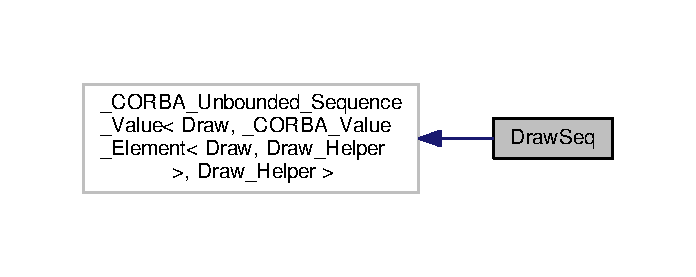
\includegraphics[width=334pt]{class_draw_seq__inherit__graph}
\end{center}
\end{figure}


Collaboration diagram for Draw\+Seq\+:
\nopagebreak
\begin{figure}[H]
\begin{center}
\leavevmode
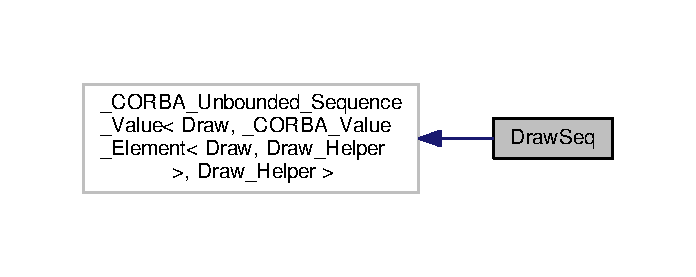
\includegraphics[width=334pt]{class_draw_seq__coll__graph}
\end{center}
\end{figure}
\subsection*{Public Types}
\begin{DoxyCompactItemize}
\item 
typedef \hyperlink{class_draw_seq__var}{Draw\+Seq\+\_\+var} \hyperlink{class_draw_seq_a588817eec2a28116ab4b5c32cbcdbd53}{\+\_\+var\+\_\+type}
\end{DoxyCompactItemize}
\subsection*{Public Member Functions}
\begin{DoxyCompactItemize}
\item 
\hyperlink{class_draw_seq_ab6753d8981b45e6ae4489d563853ccd3}{Draw\+Seq} ()
\item 
\hyperlink{class_draw_seq_a2f5903fb71c83ac0b55cb9d007c416f1}{Draw\+Seq} (const \hyperlink{class_draw_seq}{Draw\+Seq} \&\+\_\+s)
\item 
\hyperlink{class_draw_seq_a82f0808b50ee619fe9fbdfa9b494c58e}{Draw\+Seq} (\+\_\+\+C\+O\+R\+B\+A\+\_\+\+U\+Long \+\_\+max)
\item 
\hyperlink{class_draw_seq_a250aa6ac36a17eace7e8160a7cc04d9e}{Draw\+Seq} (\+\_\+\+C\+O\+R\+B\+A\+\_\+\+U\+Long \+\_\+max, \+\_\+\+C\+O\+R\+B\+A\+\_\+\+U\+Long \+\_\+len, \hyperlink{class_draw}{Draw} $\ast$$\ast$\+\_\+val, \+\_\+\+C\+O\+R\+B\+A\+\_\+\+Boolean \+\_\+rel=0)
\item 
\hyperlink{class_draw_seq}{Draw\+Seq} \& \hyperlink{class_draw_seq_a761bc56785aa9355562aebe6d429c19a}{operator=} (const \hyperlink{class_draw_seq}{Draw\+Seq} \&\+\_\+s)
\end{DoxyCompactItemize}


\subsection{Detailed Description}


Definition at line 104 of file Petit\+Prince.\+hpp.



\subsection{Member Typedef Documentation}
\index{Draw\+Seq@{Draw\+Seq}!\+\_\+var\+\_\+type@{\+\_\+var\+\_\+type}}
\index{\+\_\+var\+\_\+type@{\+\_\+var\+\_\+type}!Draw\+Seq@{Draw\+Seq}}
\subsubsection[{\texorpdfstring{\+\_\+var\+\_\+type}{_var_type}}]{\setlength{\rightskip}{0pt plus 5cm}typedef {\bf Draw\+Seq\+\_\+var} {\bf Draw\+Seq\+::\+\_\+var\+\_\+type}}\hypertarget{class_draw_seq_a588817eec2a28116ab4b5c32cbcdbd53}{}\label{class_draw_seq_a588817eec2a28116ab4b5c32cbcdbd53}


Definition at line 106 of file Petit\+Prince.\+hpp.



\subsection{Constructor \& Destructor Documentation}
\index{Draw\+Seq@{Draw\+Seq}!Draw\+Seq@{Draw\+Seq}}
\index{Draw\+Seq@{Draw\+Seq}!Draw\+Seq@{Draw\+Seq}}
\subsubsection[{\texorpdfstring{Draw\+Seq()}{DrawSeq()}}]{\setlength{\rightskip}{0pt plus 5cm}Draw\+Seq\+::\+Draw\+Seq (
\begin{DoxyParamCaption}
{}
\end{DoxyParamCaption}
)\hspace{0.3cm}{\ttfamily [inline]}}\hypertarget{class_draw_seq_ab6753d8981b45e6ae4489d563853ccd3}{}\label{class_draw_seq_ab6753d8981b45e6ae4489d563853ccd3}


Definition at line 107 of file Petit\+Prince.\+hpp.

\index{Draw\+Seq@{Draw\+Seq}!Draw\+Seq@{Draw\+Seq}}
\index{Draw\+Seq@{Draw\+Seq}!Draw\+Seq@{Draw\+Seq}}
\subsubsection[{\texorpdfstring{Draw\+Seq(const Draw\+Seq \&\+\_\+s)}{DrawSeq(const DrawSeq &_s)}}]{\setlength{\rightskip}{0pt plus 5cm}Draw\+Seq\+::\+Draw\+Seq (
\begin{DoxyParamCaption}
\item[{const {\bf Draw\+Seq} \&}]{\+\_\+s}
\end{DoxyParamCaption}
)\hspace{0.3cm}{\ttfamily [inline]}}\hypertarget{class_draw_seq_a2f5903fb71c83ac0b55cb9d007c416f1}{}\label{class_draw_seq_a2f5903fb71c83ac0b55cb9d007c416f1}


Definition at line 108 of file Petit\+Prince.\+hpp.

\index{Draw\+Seq@{Draw\+Seq}!Draw\+Seq@{Draw\+Seq}}
\index{Draw\+Seq@{Draw\+Seq}!Draw\+Seq@{Draw\+Seq}}
\subsubsection[{\texorpdfstring{Draw\+Seq(\+\_\+\+C\+O\+R\+B\+A\+\_\+\+U\+Long \+\_\+max)}{DrawSeq(_CORBA_ULong _max)}}]{\setlength{\rightskip}{0pt plus 5cm}Draw\+Seq\+::\+Draw\+Seq (
\begin{DoxyParamCaption}
\item[{\+\_\+\+C\+O\+R\+B\+A\+\_\+\+U\+Long}]{\+\_\+max}
\end{DoxyParamCaption}
)\hspace{0.3cm}{\ttfamily [inline]}}\hypertarget{class_draw_seq_a82f0808b50ee619fe9fbdfa9b494c58e}{}\label{class_draw_seq_a82f0808b50ee619fe9fbdfa9b494c58e}


Definition at line 111 of file Petit\+Prince.\+hpp.

\index{Draw\+Seq@{Draw\+Seq}!Draw\+Seq@{Draw\+Seq}}
\index{Draw\+Seq@{Draw\+Seq}!Draw\+Seq@{Draw\+Seq}}
\subsubsection[{\texorpdfstring{Draw\+Seq(\+\_\+\+C\+O\+R\+B\+A\+\_\+\+U\+Long \+\_\+max, \+\_\+\+C\+O\+R\+B\+A\+\_\+\+U\+Long \+\_\+len, Draw $\ast$$\ast$\+\_\+val, \+\_\+\+C\+O\+R\+B\+A\+\_\+\+Boolean \+\_\+rel=0)}{DrawSeq(_CORBA_ULong _max, _CORBA_ULong _len, Draw **_val, _CORBA_Boolean _rel=0)}}]{\setlength{\rightskip}{0pt plus 5cm}Draw\+Seq\+::\+Draw\+Seq (
\begin{DoxyParamCaption}
\item[{\+\_\+\+C\+O\+R\+B\+A\+\_\+\+U\+Long}]{\+\_\+max, }
\item[{\+\_\+\+C\+O\+R\+B\+A\+\_\+\+U\+Long}]{\+\_\+len, }
\item[{{\bf Draw} $\ast$$\ast$}]{\+\_\+val, }
\item[{\+\_\+\+C\+O\+R\+B\+A\+\_\+\+Boolean}]{\+\_\+rel = {\ttfamily 0}}
\end{DoxyParamCaption}
)\hspace{0.3cm}{\ttfamily [inline]}}\hypertarget{class_draw_seq_a250aa6ac36a17eace7e8160a7cc04d9e}{}\label{class_draw_seq_a250aa6ac36a17eace7e8160a7cc04d9e}


Definition at line 113 of file Petit\+Prince.\+hpp.



\subsection{Member Function Documentation}
\index{Draw\+Seq@{Draw\+Seq}!operator=@{operator=}}
\index{operator=@{operator=}!Draw\+Seq@{Draw\+Seq}}
\subsubsection[{\texorpdfstring{operator=(const Draw\+Seq \&\+\_\+s)}{operator=(const DrawSeq &_s)}}]{\setlength{\rightskip}{0pt plus 5cm}{\bf Draw\+Seq}\& Draw\+Seq\+::operator= (
\begin{DoxyParamCaption}
\item[{const {\bf Draw\+Seq} \&}]{\+\_\+s}
\end{DoxyParamCaption}
)\hspace{0.3cm}{\ttfamily [inline]}}\hypertarget{class_draw_seq_a761bc56785aa9355562aebe6d429c19a}{}\label{class_draw_seq_a761bc56785aa9355562aebe6d429c19a}


Definition at line 118 of file Petit\+Prince.\+hpp.



The documentation for this class was generated from the following file\+:\begin{DoxyCompactItemize}
\item 
hdr/\hyperlink{_petit_prince_8hpp}{Petit\+Prince.\+hpp}\end{DoxyCompactItemize}

\hypertarget{class_draw_seq__out}{}\section{Draw\+Seq\+\_\+out Class Reference}
\label{class_draw_seq__out}\index{Draw\+Seq\+\_\+out@{Draw\+Seq\+\_\+out}}


{\ttfamily \#include $<$Petit\+Prince.\+hpp$>$}



Collaboration diagram for Draw\+Seq\+\_\+out\+:
\nopagebreak
\begin{figure}[H]
\begin{center}
\leavevmode
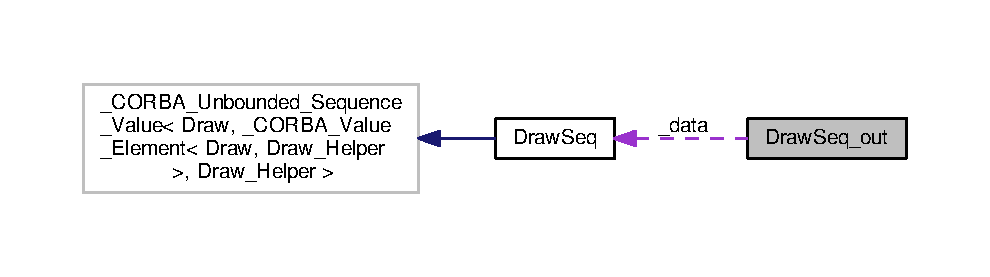
\includegraphics[width=350pt]{class_draw_seq__out__coll__graph}
\end{center}
\end{figure}
\subsection*{Public Member Functions}
\begin{DoxyCompactItemize}
\item 
\hyperlink{class_draw_seq__out_a3bcf2290b7ec119dd19ccf5b377c1aa1}{Draw\+Seq\+\_\+out} (\hyperlink{class_draw_seq}{Draw\+Seq} $\ast$\&\+\_\+s)
\item 
\hyperlink{class_draw_seq__out_a9aa391f0c2e359b622ca004de2febf74}{Draw\+Seq\+\_\+out} (\hyperlink{class_draw_seq__var}{Draw\+Seq\+\_\+var} \&\+\_\+s)
\item 
\hyperlink{class_draw_seq__out_ad924617c29ae2842379aa377c5ff797f}{Draw\+Seq\+\_\+out} (const \hyperlink{class_draw_seq__out}{Draw\+Seq\+\_\+out} \&\+\_\+s)
\item 
\hyperlink{class_draw_seq__out}{Draw\+Seq\+\_\+out} \& \hyperlink{class_draw_seq__out_a94b4fa040ba74b352f90918383cb7ff8}{operator=} (const \hyperlink{class_draw_seq__out}{Draw\+Seq\+\_\+out} \&\+\_\+s)
\item 
\hyperlink{class_draw_seq__out}{Draw\+Seq\+\_\+out} \& \hyperlink{class_draw_seq__out_ac27b922495c2dacebe0a4f92dc66c937}{operator=} (\hyperlink{class_draw_seq}{Draw\+Seq} $\ast$\+\_\+s)
\item 
\hyperlink{class_draw_seq__out_afe73ef013d4a5d6c843e6c3ff2dbfe98}{operator Draw\+Seq $\ast$\&} ()
\item 
\hyperlink{class_draw_seq}{Draw\+Seq} $\ast$\& \hyperlink{class_draw_seq__out_aa2723e52af6f4aecd33f619ffb3f9205}{ptr} ()
\item 
\hyperlink{class_draw_seq}{Draw\+Seq} $\ast$ \hyperlink{class_draw_seq__out_ac5275d7c723608533feb25d9def2b9cd}{operator-\/$>$} ()
\item 
\+\_\+\+C\+O\+R\+B\+A\+\_\+\+Value\+\_\+\+Element$<$ \hyperlink{class_draw}{Draw}, \hyperlink{class_draw___helper}{Draw\+\_\+\+Helper} $>$ \hyperlink{class_draw_seq__out_ade588ecd45acfb9aacbf9cdc58464c42}{operator\mbox{[}$\,$\mbox{]}} (\+\_\+\+C\+O\+R\+B\+A\+\_\+\+U\+Long \+\_\+i)
\end{DoxyCompactItemize}
\subsection*{Public Attributes}
\begin{DoxyCompactItemize}
\item 
\hyperlink{class_draw_seq}{Draw\+Seq} $\ast$\& \hyperlink{class_draw_seq__out_a84073e66bec09b833c5c11ff7cac2d18}{\+\_\+data}
\end{DoxyCompactItemize}


\subsection{Constructor \& Destructor Documentation}
\index{Draw\+Seq\+\_\+out@{Draw\+Seq\+\_\+out}!Draw\+Seq\+\_\+out@{Draw\+Seq\+\_\+out}}
\index{Draw\+Seq\+\_\+out@{Draw\+Seq\+\_\+out}!Draw\+Seq\+\_\+out@{Draw\+Seq\+\_\+out}}
\subsubsection[{\texorpdfstring{Draw\+Seq\+\_\+out(\+Draw\+Seq $\ast$\&\+\_\+s)}{DrawSeq_out(DrawSeq *&_s)}}]{\setlength{\rightskip}{0pt plus 5cm}Draw\+Seq\+\_\+out\+::\+Draw\+Seq\+\_\+out (
\begin{DoxyParamCaption}
\item[{{\bf Draw\+Seq} $\ast$\&}]{\+\_\+s}
\end{DoxyParamCaption}
)\hspace{0.3cm}{\ttfamily [inline]}}\hypertarget{class_draw_seq__out_a3bcf2290b7ec119dd19ccf5b377c1aa1}{}\label{class_draw_seq__out_a3bcf2290b7ec119dd19ccf5b377c1aa1}
\index{Draw\+Seq\+\_\+out@{Draw\+Seq\+\_\+out}!Draw\+Seq\+\_\+out@{Draw\+Seq\+\_\+out}}
\index{Draw\+Seq\+\_\+out@{Draw\+Seq\+\_\+out}!Draw\+Seq\+\_\+out@{Draw\+Seq\+\_\+out}}
\subsubsection[{\texorpdfstring{Draw\+Seq\+\_\+out(\+Draw\+Seq\+\_\+var \&\+\_\+s)}{DrawSeq_out(DrawSeq_var &_s)}}]{\setlength{\rightskip}{0pt plus 5cm}Draw\+Seq\+\_\+out\+::\+Draw\+Seq\+\_\+out (
\begin{DoxyParamCaption}
\item[{{\bf Draw\+Seq\+\_\+var} \&}]{\+\_\+s}
\end{DoxyParamCaption}
)\hspace{0.3cm}{\ttfamily [inline]}}\hypertarget{class_draw_seq__out_a9aa391f0c2e359b622ca004de2febf74}{}\label{class_draw_seq__out_a9aa391f0c2e359b622ca004de2febf74}
\index{Draw\+Seq\+\_\+out@{Draw\+Seq\+\_\+out}!Draw\+Seq\+\_\+out@{Draw\+Seq\+\_\+out}}
\index{Draw\+Seq\+\_\+out@{Draw\+Seq\+\_\+out}!Draw\+Seq\+\_\+out@{Draw\+Seq\+\_\+out}}
\subsubsection[{\texorpdfstring{Draw\+Seq\+\_\+out(const Draw\+Seq\+\_\+out \&\+\_\+s)}{DrawSeq_out(const DrawSeq_out &_s)}}]{\setlength{\rightskip}{0pt plus 5cm}Draw\+Seq\+\_\+out\+::\+Draw\+Seq\+\_\+out (
\begin{DoxyParamCaption}
\item[{const {\bf Draw\+Seq\+\_\+out} \&}]{\+\_\+s}
\end{DoxyParamCaption}
)\hspace{0.3cm}{\ttfamily [inline]}}\hypertarget{class_draw_seq__out_ad924617c29ae2842379aa377c5ff797f}{}\label{class_draw_seq__out_ad924617c29ae2842379aa377c5ff797f}


\subsection{Member Function Documentation}
\index{Draw\+Seq\+\_\+out@{Draw\+Seq\+\_\+out}!operator Draw\+Seq $\ast$\&@{operator Draw\+Seq $\ast$\&}}
\index{operator Draw\+Seq $\ast$\&@{operator Draw\+Seq $\ast$\&}!Draw\+Seq\+\_\+out@{Draw\+Seq\+\_\+out}}
\subsubsection[{\texorpdfstring{operator Draw\+Seq $\ast$\&()}{operator DrawSeq *&()}}]{\setlength{\rightskip}{0pt plus 5cm}Draw\+Seq\+\_\+out\+::operator {\bf Draw\+Seq} $\ast$\& (
\begin{DoxyParamCaption}
{}
\end{DoxyParamCaption}
)\hspace{0.3cm}{\ttfamily [inline]}}\hypertarget{class_draw_seq__out_afe73ef013d4a5d6c843e6c3ff2dbfe98}{}\label{class_draw_seq__out_afe73ef013d4a5d6c843e6c3ff2dbfe98}
\index{Draw\+Seq\+\_\+out@{Draw\+Seq\+\_\+out}!operator-\/$>$@{operator-\/$>$}}
\index{operator-\/$>$@{operator-\/$>$}!Draw\+Seq\+\_\+out@{Draw\+Seq\+\_\+out}}
\subsubsection[{\texorpdfstring{operator-\/$>$()}{operator->()}}]{\setlength{\rightskip}{0pt plus 5cm}{\bf Draw\+Seq}$\ast$ Draw\+Seq\+\_\+out\+::operator-\/$>$ (
\begin{DoxyParamCaption}
{}
\end{DoxyParamCaption}
)\hspace{0.3cm}{\ttfamily [inline]}}\hypertarget{class_draw_seq__out_ac5275d7c723608533feb25d9def2b9cd}{}\label{class_draw_seq__out_ac5275d7c723608533feb25d9def2b9cd}
\index{Draw\+Seq\+\_\+out@{Draw\+Seq\+\_\+out}!operator=@{operator=}}
\index{operator=@{operator=}!Draw\+Seq\+\_\+out@{Draw\+Seq\+\_\+out}}
\subsubsection[{\texorpdfstring{operator=(const Draw\+Seq\+\_\+out \&\+\_\+s)}{operator=(const DrawSeq_out &_s)}}]{\setlength{\rightskip}{0pt plus 5cm}{\bf Draw\+Seq\+\_\+out}\& Draw\+Seq\+\_\+out\+::operator= (
\begin{DoxyParamCaption}
\item[{const {\bf Draw\+Seq\+\_\+out} \&}]{\+\_\+s}
\end{DoxyParamCaption}
)\hspace{0.3cm}{\ttfamily [inline]}}\hypertarget{class_draw_seq__out_a94b4fa040ba74b352f90918383cb7ff8}{}\label{class_draw_seq__out_a94b4fa040ba74b352f90918383cb7ff8}
\index{Draw\+Seq\+\_\+out@{Draw\+Seq\+\_\+out}!operator=@{operator=}}
\index{operator=@{operator=}!Draw\+Seq\+\_\+out@{Draw\+Seq\+\_\+out}}
\subsubsection[{\texorpdfstring{operator=(\+Draw\+Seq $\ast$\+\_\+s)}{operator=(DrawSeq *_s)}}]{\setlength{\rightskip}{0pt plus 5cm}{\bf Draw\+Seq\+\_\+out}\& Draw\+Seq\+\_\+out\+::operator= (
\begin{DoxyParamCaption}
\item[{{\bf Draw\+Seq} $\ast$}]{\+\_\+s}
\end{DoxyParamCaption}
)\hspace{0.3cm}{\ttfamily [inline]}}\hypertarget{class_draw_seq__out_ac27b922495c2dacebe0a4f92dc66c937}{}\label{class_draw_seq__out_ac27b922495c2dacebe0a4f92dc66c937}
\index{Draw\+Seq\+\_\+out@{Draw\+Seq\+\_\+out}!operator\mbox{[}$\,$\mbox{]}@{operator[]}}
\index{operator\mbox{[}$\,$\mbox{]}@{operator[]}!Draw\+Seq\+\_\+out@{Draw\+Seq\+\_\+out}}
\subsubsection[{\texorpdfstring{operator[](\+\_\+\+C\+O\+R\+B\+A\+\_\+\+U\+Long \+\_\+i)}{operator[](_CORBA_ULong _i)}}]{\setlength{\rightskip}{0pt plus 5cm}\+\_\+\+C\+O\+R\+B\+A\+\_\+\+Value\+\_\+\+Element$<$ {\bf Draw}, {\bf Draw\+\_\+\+Helper} $>$ Draw\+Seq\+\_\+out\+::operator\mbox{[}$\,$\mbox{]} (
\begin{DoxyParamCaption}
\item[{\+\_\+\+C\+O\+R\+B\+A\+\_\+\+U\+Long}]{\+\_\+i}
\end{DoxyParamCaption}
)\hspace{0.3cm}{\ttfamily [inline]}}\hypertarget{class_draw_seq__out_ade588ecd45acfb9aacbf9cdc58464c42}{}\label{class_draw_seq__out_ade588ecd45acfb9aacbf9cdc58464c42}
\index{Draw\+Seq\+\_\+out@{Draw\+Seq\+\_\+out}!ptr@{ptr}}
\index{ptr@{ptr}!Draw\+Seq\+\_\+out@{Draw\+Seq\+\_\+out}}
\subsubsection[{\texorpdfstring{ptr()}{ptr()}}]{\setlength{\rightskip}{0pt plus 5cm}{\bf Draw\+Seq}$\ast$\& Draw\+Seq\+\_\+out\+::ptr (
\begin{DoxyParamCaption}
{}
\end{DoxyParamCaption}
)\hspace{0.3cm}{\ttfamily [inline]}}\hypertarget{class_draw_seq__out_aa2723e52af6f4aecd33f619ffb3f9205}{}\label{class_draw_seq__out_aa2723e52af6f4aecd33f619ffb3f9205}


\subsection{Member Data Documentation}
\index{Draw\+Seq\+\_\+out@{Draw\+Seq\+\_\+out}!\+\_\+data@{\+\_\+data}}
\index{\+\_\+data@{\+\_\+data}!Draw\+Seq\+\_\+out@{Draw\+Seq\+\_\+out}}
\subsubsection[{\texorpdfstring{\+\_\+data}{_data}}]{\setlength{\rightskip}{0pt plus 5cm}{\bf Draw\+Seq}$\ast$\& Draw\+Seq\+\_\+out\+::\+\_\+data}\hypertarget{class_draw_seq__out_a84073e66bec09b833c5c11ff7cac2d18}{}\label{class_draw_seq__out_a84073e66bec09b833c5c11ff7cac2d18}


The documentation for this class was generated from the following file\+:\begin{DoxyCompactItemize}
\item 
hdr/\hyperlink{_petit_prince_8hpp}{Petit\+Prince.\+hpp}\end{DoxyCompactItemize}

\hypertarget{class_draw_seq__var}{}\section{Draw\+Seq\+\_\+var Class Reference}
\label{class_draw_seq__var}\index{Draw\+Seq\+\_\+var@{Draw\+Seq\+\_\+var}}


{\ttfamily \#include $<$Petit\+Prince.\+hpp$>$}

\subsection*{Public Member Functions}
\begin{DoxyCompactItemize}
\item 
\hyperlink{class_draw_seq__var_a4518ea24553a2aafd836c006c26a9fff}{Draw\+Seq\+\_\+var} ()
\item 
\hyperlink{class_draw_seq__var_aeebfb914d20643d8702d68316d5e0d7d}{Draw\+Seq\+\_\+var} (\hyperlink{class_draw_seq}{Draw\+Seq} $\ast$\+\_\+s)
\item 
\hyperlink{class_draw_seq__var_a0292cb4e4593865dde71c1935c91f23e}{Draw\+Seq\+\_\+var} (const \hyperlink{class_draw_seq__var}{Draw\+Seq\+\_\+var} \&\+\_\+s)
\item 
\hyperlink{class_draw_seq__var_ad50acfa35f8eb735d8ec4ae89036df7a}{$\sim$\+Draw\+Seq\+\_\+var} ()
\item 
\hyperlink{class_draw_seq__var}{Draw\+Seq\+\_\+var} \& \hyperlink{class_draw_seq__var_ae2163957cae0c0c7ad29fc8f0d1c2e73}{operator=} (\hyperlink{class_draw_seq}{Draw\+Seq} $\ast$\+\_\+s)
\item 
\hyperlink{class_draw_seq__var}{Draw\+Seq\+\_\+var} \& \hyperlink{class_draw_seq__var_a7552db5e6ff6519dbba182d5166fc74c}{operator=} (const \hyperlink{class_draw_seq__var}{Draw\+Seq\+\_\+var} \&\+\_\+s)
\item 
\+\_\+\+C\+O\+R\+B\+A\+\_\+\+Value\+\_\+\+Element$<$ \hyperlink{class_draw}{Draw}, \hyperlink{class_draw___helper}{Draw\+\_\+\+Helper} $>$ \hyperlink{class_draw_seq__var_a75adf5f5bc9cf4bb1027c7cbcc53005e}{operator\mbox{[}$\,$\mbox{]}} (\+\_\+\+C\+O\+R\+B\+A\+\_\+\+U\+Long \+\_\+s)
\item 
\hyperlink{class_draw_seq}{Draw\+Seq} $\ast$ \hyperlink{class_draw_seq__var_a8d10efff3b1c9a5a0ca4bc94a024d430}{operator-\/$>$} ()
\item 
const \hyperlink{class_draw_seq}{Draw\+Seq} $\ast$ \hyperlink{class_draw_seq__var_ac4fb1a0e5aa99f10f07c58c5e1d66548}{operator-\/$>$} () const 
\item 
\hyperlink{class_draw_seq__var_a0017de47bcba701ac41fd21b54a1dc62}{operator const Draw\+Seq \&} () const 
\item 
\hyperlink{class_draw_seq__var_a87f6835a288fec43d7caffbc2e4c1f35}{operator Draw\+Seq \&} ()
\item 
const \hyperlink{class_draw_seq}{Draw\+Seq} \& \hyperlink{class_draw_seq__var_a306c0aa03c9bc5784aae2d53abdc740a}{in} () const 
\item 
\hyperlink{class_draw_seq}{Draw\+Seq} \& \hyperlink{class_draw_seq__var_a633fd2f47251e1e3f98bc3d6fbc564ac}{inout} ()
\item 
\hyperlink{class_draw_seq}{Draw\+Seq} $\ast$\& \hyperlink{class_draw_seq__var_a10a1988d47dab1026775a055373f08f2}{out} ()
\item 
\hyperlink{class_draw_seq}{Draw\+Seq} $\ast$ \hyperlink{class_draw_seq__var_a230eedc2bced84c334c3a7056597a24c}{\+\_\+retn} ()
\end{DoxyCompactItemize}
\subsection*{Friends}
\begin{DoxyCompactItemize}
\item 
class \hyperlink{class_draw_seq__var_a6ed6931575fd9d7adbdc41b34a836904}{Draw\+Seq\+\_\+out}
\end{DoxyCompactItemize}


\subsection{Constructor \& Destructor Documentation}
\index{Draw\+Seq\+\_\+var@{Draw\+Seq\+\_\+var}!Draw\+Seq\+\_\+var@{Draw\+Seq\+\_\+var}}
\index{Draw\+Seq\+\_\+var@{Draw\+Seq\+\_\+var}!Draw\+Seq\+\_\+var@{Draw\+Seq\+\_\+var}}
\subsubsection[{\texorpdfstring{Draw\+Seq\+\_\+var()}{DrawSeq_var()}}]{\setlength{\rightskip}{0pt plus 5cm}Draw\+Seq\+\_\+var\+::\+Draw\+Seq\+\_\+var (
\begin{DoxyParamCaption}
{}
\end{DoxyParamCaption}
)\hspace{0.3cm}{\ttfamily [inline]}}\hypertarget{class_draw_seq__var_a4518ea24553a2aafd836c006c26a9fff}{}\label{class_draw_seq__var_a4518ea24553a2aafd836c006c26a9fff}
\index{Draw\+Seq\+\_\+var@{Draw\+Seq\+\_\+var}!Draw\+Seq\+\_\+var@{Draw\+Seq\+\_\+var}}
\index{Draw\+Seq\+\_\+var@{Draw\+Seq\+\_\+var}!Draw\+Seq\+\_\+var@{Draw\+Seq\+\_\+var}}
\subsubsection[{\texorpdfstring{Draw\+Seq\+\_\+var(\+Draw\+Seq $\ast$\+\_\+s)}{DrawSeq_var(DrawSeq *_s)}}]{\setlength{\rightskip}{0pt plus 5cm}Draw\+Seq\+\_\+var\+::\+Draw\+Seq\+\_\+var (
\begin{DoxyParamCaption}
\item[{{\bf Draw\+Seq} $\ast$}]{\+\_\+s}
\end{DoxyParamCaption}
)\hspace{0.3cm}{\ttfamily [inline]}}\hypertarget{class_draw_seq__var_aeebfb914d20643d8702d68316d5e0d7d}{}\label{class_draw_seq__var_aeebfb914d20643d8702d68316d5e0d7d}
\index{Draw\+Seq\+\_\+var@{Draw\+Seq\+\_\+var}!Draw\+Seq\+\_\+var@{Draw\+Seq\+\_\+var}}
\index{Draw\+Seq\+\_\+var@{Draw\+Seq\+\_\+var}!Draw\+Seq\+\_\+var@{Draw\+Seq\+\_\+var}}
\subsubsection[{\texorpdfstring{Draw\+Seq\+\_\+var(const Draw\+Seq\+\_\+var \&\+\_\+s)}{DrawSeq_var(const DrawSeq_var &_s)}}]{\setlength{\rightskip}{0pt plus 5cm}Draw\+Seq\+\_\+var\+::\+Draw\+Seq\+\_\+var (
\begin{DoxyParamCaption}
\item[{const {\bf Draw\+Seq\+\_\+var} \&}]{\+\_\+s}
\end{DoxyParamCaption}
)\hspace{0.3cm}{\ttfamily [inline]}}\hypertarget{class_draw_seq__var_a0292cb4e4593865dde71c1935c91f23e}{}\label{class_draw_seq__var_a0292cb4e4593865dde71c1935c91f23e}
\index{Draw\+Seq\+\_\+var@{Draw\+Seq\+\_\+var}!````~Draw\+Seq\+\_\+var@{$\sim$\+Draw\+Seq\+\_\+var}}
\index{````~Draw\+Seq\+\_\+var@{$\sim$\+Draw\+Seq\+\_\+var}!Draw\+Seq\+\_\+var@{Draw\+Seq\+\_\+var}}
\subsubsection[{\texorpdfstring{$\sim$\+Draw\+Seq\+\_\+var()}{~DrawSeq_var()}}]{\setlength{\rightskip}{0pt plus 5cm}Draw\+Seq\+\_\+var\+::$\sim$\+Draw\+Seq\+\_\+var (
\begin{DoxyParamCaption}
{}
\end{DoxyParamCaption}
)\hspace{0.3cm}{\ttfamily [inline]}}\hypertarget{class_draw_seq__var_ad50acfa35f8eb735d8ec4ae89036df7a}{}\label{class_draw_seq__var_ad50acfa35f8eb735d8ec4ae89036df7a}


\subsection{Member Function Documentation}
\index{Draw\+Seq\+\_\+var@{Draw\+Seq\+\_\+var}!\+\_\+retn@{\+\_\+retn}}
\index{\+\_\+retn@{\+\_\+retn}!Draw\+Seq\+\_\+var@{Draw\+Seq\+\_\+var}}
\subsubsection[{\texorpdfstring{\+\_\+retn()}{_retn()}}]{\setlength{\rightskip}{0pt plus 5cm}{\bf Draw\+Seq}$\ast$ Draw\+Seq\+\_\+var\+::\+\_\+retn (
\begin{DoxyParamCaption}
{}
\end{DoxyParamCaption}
)\hspace{0.3cm}{\ttfamily [inline]}}\hypertarget{class_draw_seq__var_a230eedc2bced84c334c3a7056597a24c}{}\label{class_draw_seq__var_a230eedc2bced84c334c3a7056597a24c}
\index{Draw\+Seq\+\_\+var@{Draw\+Seq\+\_\+var}!in@{in}}
\index{in@{in}!Draw\+Seq\+\_\+var@{Draw\+Seq\+\_\+var}}
\subsubsection[{\texorpdfstring{in() const }{in() const }}]{\setlength{\rightskip}{0pt plus 5cm}const {\bf Draw\+Seq}\& Draw\+Seq\+\_\+var\+::in (
\begin{DoxyParamCaption}
{}
\end{DoxyParamCaption}
) const\hspace{0.3cm}{\ttfamily [inline]}}\hypertarget{class_draw_seq__var_a306c0aa03c9bc5784aae2d53abdc740a}{}\label{class_draw_seq__var_a306c0aa03c9bc5784aae2d53abdc740a}
\index{Draw\+Seq\+\_\+var@{Draw\+Seq\+\_\+var}!inout@{inout}}
\index{inout@{inout}!Draw\+Seq\+\_\+var@{Draw\+Seq\+\_\+var}}
\subsubsection[{\texorpdfstring{inout()}{inout()}}]{\setlength{\rightskip}{0pt plus 5cm}{\bf Draw\+Seq}\& Draw\+Seq\+\_\+var\+::inout (
\begin{DoxyParamCaption}
{}
\end{DoxyParamCaption}
)\hspace{0.3cm}{\ttfamily [inline]}}\hypertarget{class_draw_seq__var_a633fd2f47251e1e3f98bc3d6fbc564ac}{}\label{class_draw_seq__var_a633fd2f47251e1e3f98bc3d6fbc564ac}
\index{Draw\+Seq\+\_\+var@{Draw\+Seq\+\_\+var}!operator const Draw\+Seq \&@{operator const Draw\+Seq \&}}
\index{operator const Draw\+Seq \&@{operator const Draw\+Seq \&}!Draw\+Seq\+\_\+var@{Draw\+Seq\+\_\+var}}
\subsubsection[{\texorpdfstring{operator const Draw\+Seq \&() const }{operator const DrawSeq &() const }}]{\setlength{\rightskip}{0pt plus 5cm}Draw\+Seq\+\_\+var\+::operator const {\bf Draw\+Seq} \& (
\begin{DoxyParamCaption}
{}
\end{DoxyParamCaption}
) const\hspace{0.3cm}{\ttfamily [inline]}}\hypertarget{class_draw_seq__var_a0017de47bcba701ac41fd21b54a1dc62}{}\label{class_draw_seq__var_a0017de47bcba701ac41fd21b54a1dc62}
\index{Draw\+Seq\+\_\+var@{Draw\+Seq\+\_\+var}!operator Draw\+Seq \&@{operator Draw\+Seq \&}}
\index{operator Draw\+Seq \&@{operator Draw\+Seq \&}!Draw\+Seq\+\_\+var@{Draw\+Seq\+\_\+var}}
\subsubsection[{\texorpdfstring{operator Draw\+Seq \&()}{operator DrawSeq &()}}]{\setlength{\rightskip}{0pt plus 5cm}Draw\+Seq\+\_\+var\+::operator {\bf Draw\+Seq} \& (
\begin{DoxyParamCaption}
{}
\end{DoxyParamCaption}
)\hspace{0.3cm}{\ttfamily [inline]}}\hypertarget{class_draw_seq__var_a87f6835a288fec43d7caffbc2e4c1f35}{}\label{class_draw_seq__var_a87f6835a288fec43d7caffbc2e4c1f35}
\index{Draw\+Seq\+\_\+var@{Draw\+Seq\+\_\+var}!operator-\/$>$@{operator-\/$>$}}
\index{operator-\/$>$@{operator-\/$>$}!Draw\+Seq\+\_\+var@{Draw\+Seq\+\_\+var}}
\subsubsection[{\texorpdfstring{operator-\/$>$()}{operator->()}}]{\setlength{\rightskip}{0pt plus 5cm}{\bf Draw\+Seq}$\ast$ Draw\+Seq\+\_\+var\+::operator-\/$>$ (
\begin{DoxyParamCaption}
{}
\end{DoxyParamCaption}
)\hspace{0.3cm}{\ttfamily [inline]}}\hypertarget{class_draw_seq__var_a8d10efff3b1c9a5a0ca4bc94a024d430}{}\label{class_draw_seq__var_a8d10efff3b1c9a5a0ca4bc94a024d430}
\index{Draw\+Seq\+\_\+var@{Draw\+Seq\+\_\+var}!operator-\/$>$@{operator-\/$>$}}
\index{operator-\/$>$@{operator-\/$>$}!Draw\+Seq\+\_\+var@{Draw\+Seq\+\_\+var}}
\subsubsection[{\texorpdfstring{operator-\/$>$() const }{operator->() const }}]{\setlength{\rightskip}{0pt plus 5cm}const {\bf Draw\+Seq}$\ast$ Draw\+Seq\+\_\+var\+::operator-\/$>$ (
\begin{DoxyParamCaption}
{}
\end{DoxyParamCaption}
) const\hspace{0.3cm}{\ttfamily [inline]}}\hypertarget{class_draw_seq__var_ac4fb1a0e5aa99f10f07c58c5e1d66548}{}\label{class_draw_seq__var_ac4fb1a0e5aa99f10f07c58c5e1d66548}
\index{Draw\+Seq\+\_\+var@{Draw\+Seq\+\_\+var}!operator=@{operator=}}
\index{operator=@{operator=}!Draw\+Seq\+\_\+var@{Draw\+Seq\+\_\+var}}
\subsubsection[{\texorpdfstring{operator=(\+Draw\+Seq $\ast$\+\_\+s)}{operator=(DrawSeq *_s)}}]{\setlength{\rightskip}{0pt plus 5cm}{\bf Draw\+Seq\+\_\+var}\& Draw\+Seq\+\_\+var\+::operator= (
\begin{DoxyParamCaption}
\item[{{\bf Draw\+Seq} $\ast$}]{\+\_\+s}
\end{DoxyParamCaption}
)\hspace{0.3cm}{\ttfamily [inline]}}\hypertarget{class_draw_seq__var_ae2163957cae0c0c7ad29fc8f0d1c2e73}{}\label{class_draw_seq__var_ae2163957cae0c0c7ad29fc8f0d1c2e73}
\index{Draw\+Seq\+\_\+var@{Draw\+Seq\+\_\+var}!operator=@{operator=}}
\index{operator=@{operator=}!Draw\+Seq\+\_\+var@{Draw\+Seq\+\_\+var}}
\subsubsection[{\texorpdfstring{operator=(const Draw\+Seq\+\_\+var \&\+\_\+s)}{operator=(const DrawSeq_var &_s)}}]{\setlength{\rightskip}{0pt plus 5cm}{\bf Draw\+Seq\+\_\+var}\& Draw\+Seq\+\_\+var\+::operator= (
\begin{DoxyParamCaption}
\item[{const {\bf Draw\+Seq\+\_\+var} \&}]{\+\_\+s}
\end{DoxyParamCaption}
)\hspace{0.3cm}{\ttfamily [inline]}}\hypertarget{class_draw_seq__var_a7552db5e6ff6519dbba182d5166fc74c}{}\label{class_draw_seq__var_a7552db5e6ff6519dbba182d5166fc74c}
\index{Draw\+Seq\+\_\+var@{Draw\+Seq\+\_\+var}!operator\mbox{[}$\,$\mbox{]}@{operator[]}}
\index{operator\mbox{[}$\,$\mbox{]}@{operator[]}!Draw\+Seq\+\_\+var@{Draw\+Seq\+\_\+var}}
\subsubsection[{\texorpdfstring{operator[](\+\_\+\+C\+O\+R\+B\+A\+\_\+\+U\+Long \+\_\+s)}{operator[](_CORBA_ULong _s)}}]{\setlength{\rightskip}{0pt plus 5cm}\+\_\+\+C\+O\+R\+B\+A\+\_\+\+Value\+\_\+\+Element$<$ {\bf Draw}, {\bf Draw\+\_\+\+Helper} $>$ Draw\+Seq\+\_\+var\+::operator\mbox{[}$\,$\mbox{]} (
\begin{DoxyParamCaption}
\item[{\+\_\+\+C\+O\+R\+B\+A\+\_\+\+U\+Long}]{\+\_\+s}
\end{DoxyParamCaption}
)\hspace{0.3cm}{\ttfamily [inline]}}\hypertarget{class_draw_seq__var_a75adf5f5bc9cf4bb1027c7cbcc53005e}{}\label{class_draw_seq__var_a75adf5f5bc9cf4bb1027c7cbcc53005e}
\index{Draw\+Seq\+\_\+var@{Draw\+Seq\+\_\+var}!out@{out}}
\index{out@{out}!Draw\+Seq\+\_\+var@{Draw\+Seq\+\_\+var}}
\subsubsection[{\texorpdfstring{out()}{out()}}]{\setlength{\rightskip}{0pt plus 5cm}{\bf Draw\+Seq}$\ast$\& Draw\+Seq\+\_\+var\+::out (
\begin{DoxyParamCaption}
{}
\end{DoxyParamCaption}
)\hspace{0.3cm}{\ttfamily [inline]}}\hypertarget{class_draw_seq__var_a10a1988d47dab1026775a055373f08f2}{}\label{class_draw_seq__var_a10a1988d47dab1026775a055373f08f2}


\subsection{Friends And Related Function Documentation}
\index{Draw\+Seq\+\_\+var@{Draw\+Seq\+\_\+var}!Draw\+Seq\+\_\+out@{Draw\+Seq\+\_\+out}}
\index{Draw\+Seq\+\_\+out@{Draw\+Seq\+\_\+out}!Draw\+Seq\+\_\+var@{Draw\+Seq\+\_\+var}}
\subsubsection[{\texorpdfstring{Draw\+Seq\+\_\+out}{DrawSeq_out}}]{\setlength{\rightskip}{0pt plus 5cm}friend class {\bf Draw\+Seq\+\_\+out}\hspace{0.3cm}{\ttfamily [friend]}}\hypertarget{class_draw_seq__var_a6ed6931575fd9d7adbdc41b34a836904}{}\label{class_draw_seq__var_a6ed6931575fd9d7adbdc41b34a836904}


The documentation for this class was generated from the following file\+:\begin{DoxyCompactItemize}
\item 
hdr/\hyperlink{_petit_prince_8hpp}{Petit\+Prince.\+hpp}\end{DoxyCompactItemize}

\hypertarget{class_draw_service}{}\section{Draw\+Service Class Reference}
\label{class_draw_service}\index{Draw\+Service@{Draw\+Service}}


{\ttfamily \#include $<$Petit\+Prince.\+hpp$>$}



Inheritance diagram for Draw\+Service\+:
\nopagebreak
\begin{figure}[H]
\begin{center}
\leavevmode
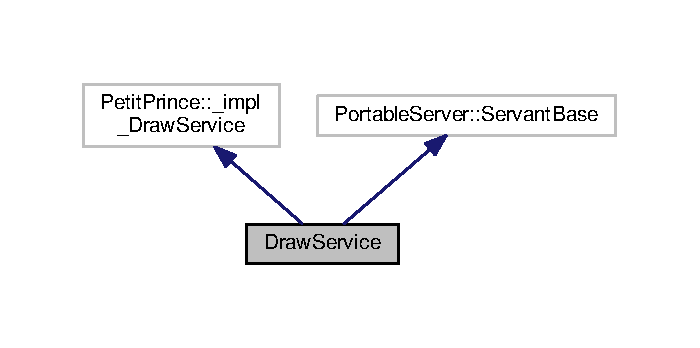
\includegraphics[width=336pt]{class_draw_service__inherit__graph}
\end{center}
\end{figure}


Collaboration diagram for Draw\+Service\+:
\nopagebreak
\begin{figure}[H]
\begin{center}
\leavevmode
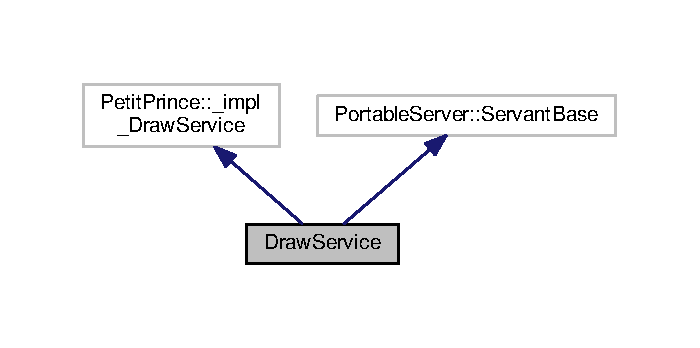
\includegraphics[width=336pt]{class_draw_service__coll__graph}
\end{center}
\end{figure}
\subsection*{Classes}
\begin{DoxyCompactItemize}
\item 
class \hyperlink{class_draw_service_1_1_non_applicable}{Non\+Applicable}
\item 
class \hyperlink{class_draw_service_1_1_unexpected_draw}{Unexpected\+Draw}
\end{DoxyCompactItemize}
\subsection*{Public Types}
\begin{DoxyCompactItemize}
\item 
typedef \hyperlink{_petit_prince_8hpp_a65d1c7d29682996870d909fc2b3b5d82}{Draw\+Service\+\_\+ptr} \hyperlink{class_draw_service_a452c5d2edf70f25bc3fb7027548adb90}{\+\_\+ptr\+\_\+type}
\item 
typedef \hyperlink{_petit_prince_8hpp_aaa2c9a4c8b5ab19df3aceb2bdd9a2275}{Draw\+Service\+\_\+var} \hyperlink{class_draw_service_a110e8421361b653ce8fca4aeefc7db2b}{\+\_\+var\+\_\+type}
\end{DoxyCompactItemize}
\subsection*{Public Member Functions}
\begin{DoxyCompactItemize}
\item 
virtual \hyperlink{class_draw_service_aac2a148525031026ad1fa42250aa25f7}{$\sim$\+Draw\+Service} ()
\item 
\hyperlink{_petit_prince_8hpp_a65d1c7d29682996870d909fc2b3b5d82}{inline\+::\+Petit\+Prince\+::\+Draw\+Service\+\_\+ptr} \hyperlink{class_draw_service_a5adf4a24cf9c7fd98b46430f3b978ad1}{\+\_\+this} ()
\end{DoxyCompactItemize}
\subsection*{Static Public Member Functions}
\begin{DoxyCompactItemize}
\item 
static \hyperlink{class_draw_service_a452c5d2edf70f25bc3fb7027548adb90}{\+\_\+ptr\+\_\+type} \hyperlink{class_draw_service_a67f18fb236cd446b03b160acf64125f3}{\+\_\+duplicate} (\hyperlink{class_draw_service_a452c5d2edf70f25bc3fb7027548adb90}{\+\_\+ptr\+\_\+type})
\item 
static \hyperlink{class_draw_service_a452c5d2edf70f25bc3fb7027548adb90}{\+\_\+ptr\+\_\+type} \hyperlink{class_draw_service_adc06ca121635bcc66b18fdf89079b236}{\+\_\+narrow} (\+::C\+O\+R\+B\+A\+::\+Object\+\_\+ptr)
\item 
static \hyperlink{class_draw_service_a452c5d2edf70f25bc3fb7027548adb90}{\+\_\+ptr\+\_\+type} \hyperlink{class_draw_service_a7c98c12c713160b6e067214d5e9046ff}{\+\_\+unchecked\+\_\+narrow} (\+::C\+O\+R\+B\+A\+::\+Object\+\_\+ptr)
\item 
static \hyperlink{class_draw_service_a452c5d2edf70f25bc3fb7027548adb90}{\+\_\+ptr\+\_\+type} \hyperlink{class_draw_service_a06f3c379539862c0e199ed6a36fc5f4a}{\+\_\+nil} ()
\item 
static void \hyperlink{class_draw_service_a4b4dbca9f78fe084a3a340bb0f4dd9ee}{\+\_\+marshal\+Obj\+Ref} (\hyperlink{class_draw_service_a452c5d2edf70f25bc3fb7027548adb90}{\+\_\+ptr\+\_\+type}, cdr\+Stream \&)
\item 
static \hyperlink{class_draw_service_a452c5d2edf70f25bc3fb7027548adb90}{\+\_\+ptr\+\_\+type} \hyperlink{class_draw_service_aad9e95aa1b6f345b50a56f9136d67d48}{\+\_\+unmarshal\+Obj\+Ref} (cdr\+Stream \&s)
\end{DoxyCompactItemize}
\subsection*{Static Public Attributes}
\begin{DoxyCompactItemize}
\item 
static \hyperlink{_petit_prince_8hpp_a5f7bf7cddb608c2aad7c95f55f8a33c5}{\+\_\+core\+\_\+attr} const char $\ast$ \hyperlink{class_draw_service_afba77735caed0164a1f53ddec6a5095a}{\+\_\+\+P\+D\+\_\+repo\+Id}
\item 
static \+\_\+dyn\+\_\+attrconst\+::\+C\+O\+R\+B\+A\+::\+Type\+Code\+\_\+ptr \hyperlink{class_draw_service_a61c64267972c67512380625107b4c42b}{\+\_\+tc\+\_\+\+Non\+Applicable}
\item 
static \+\_\+dyn\+\_\+attrconst\+::\+C\+O\+R\+B\+A\+::\+Type\+Code\+\_\+ptr \hyperlink{class_draw_service_a20a8de19b0f9d322579bf636ca2dd1e6}{\+\_\+tc\+\_\+\+Unexpected\+Draw}
\end{DoxyCompactItemize}


\subsection{Member Typedef Documentation}
\index{Draw\+Service@{Draw\+Service}!\+\_\+ptr\+\_\+type@{\+\_\+ptr\+\_\+type}}
\index{\+\_\+ptr\+\_\+type@{\+\_\+ptr\+\_\+type}!Draw\+Service@{Draw\+Service}}
\subsubsection[{\texorpdfstring{\+\_\+ptr\+\_\+type}{_ptr_type}}]{\setlength{\rightskip}{0pt plus 5cm}typedef {\bf Draw\+Service\+\_\+ptr} {\bf Draw\+Service\+::\+\_\+ptr\+\_\+type}}\hypertarget{class_draw_service_a452c5d2edf70f25bc3fb7027548adb90}{}\label{class_draw_service_a452c5d2edf70f25bc3fb7027548adb90}
\index{Draw\+Service@{Draw\+Service}!\+\_\+var\+\_\+type@{\+\_\+var\+\_\+type}}
\index{\+\_\+var\+\_\+type@{\+\_\+var\+\_\+type}!Draw\+Service@{Draw\+Service}}
\subsubsection[{\texorpdfstring{\+\_\+var\+\_\+type}{_var_type}}]{\setlength{\rightskip}{0pt plus 5cm}typedef {\bf Draw\+Service\+\_\+var} {\bf Draw\+Service\+::\+\_\+var\+\_\+type}}\hypertarget{class_draw_service_a110e8421361b653ce8fca4aeefc7db2b}{}\label{class_draw_service_a110e8421361b653ce8fca4aeefc7db2b}


\subsection{Constructor \& Destructor Documentation}
\index{Draw\+Service@{Draw\+Service}!````~Draw\+Service@{$\sim$\+Draw\+Service}}
\index{````~Draw\+Service@{$\sim$\+Draw\+Service}!Draw\+Service@{Draw\+Service}}
\subsubsection[{\texorpdfstring{$\sim$\+Draw\+Service()}{~DrawService()}}]{\setlength{\rightskip}{0pt plus 5cm}virtual Draw\+Service\+::$\sim$\+Draw\+Service (
\begin{DoxyParamCaption}
{}
\end{DoxyParamCaption}
)\hspace{0.3cm}{\ttfamily [virtual]}}\hypertarget{class_draw_service_aac2a148525031026ad1fa42250aa25f7}{}\label{class_draw_service_aac2a148525031026ad1fa42250aa25f7}


\subsection{Member Function Documentation}
\index{Draw\+Service@{Draw\+Service}!\+\_\+duplicate@{\+\_\+duplicate}}
\index{\+\_\+duplicate@{\+\_\+duplicate}!Draw\+Service@{Draw\+Service}}
\subsubsection[{\texorpdfstring{\+\_\+duplicate(\+\_\+ptr\+\_\+type)}{_duplicate(_ptr_type)}}]{\setlength{\rightskip}{0pt plus 5cm}static {\bf \+\_\+ptr\+\_\+type} Draw\+Service\+::\+\_\+duplicate (
\begin{DoxyParamCaption}
\item[{{\bf \+\_\+ptr\+\_\+type}}]{}
\end{DoxyParamCaption}
)\hspace{0.3cm}{\ttfamily [static]}}\hypertarget{class_draw_service_a67f18fb236cd446b03b160acf64125f3}{}\label{class_draw_service_a67f18fb236cd446b03b160acf64125f3}
\index{Draw\+Service@{Draw\+Service}!\+\_\+marshal\+Obj\+Ref@{\+\_\+marshal\+Obj\+Ref}}
\index{\+\_\+marshal\+Obj\+Ref@{\+\_\+marshal\+Obj\+Ref}!Draw\+Service@{Draw\+Service}}
\subsubsection[{\texorpdfstring{\+\_\+marshal\+Obj\+Ref(\+\_\+ptr\+\_\+type, cdr\+Stream \&)}{_marshalObjRef(_ptr_type, cdrStream &)}}]{\setlength{\rightskip}{0pt plus 5cm}static void Draw\+Service\+::\+\_\+marshal\+Obj\+Ref (
\begin{DoxyParamCaption}
\item[{{\bf \+\_\+ptr\+\_\+type}}]{, }
\item[{cdr\+Stream \&}]{}
\end{DoxyParamCaption}
)\hspace{0.3cm}{\ttfamily [inline]}, {\ttfamily [static]}}\hypertarget{class_draw_service_a4b4dbca9f78fe084a3a340bb0f4dd9ee}{}\label{class_draw_service_a4b4dbca9f78fe084a3a340bb0f4dd9ee}
\index{Draw\+Service@{Draw\+Service}!\+\_\+narrow@{\+\_\+narrow}}
\index{\+\_\+narrow@{\+\_\+narrow}!Draw\+Service@{Draw\+Service}}
\subsubsection[{\texorpdfstring{\+\_\+narrow(\+::\+C\+O\+R\+B\+A\+::\+Object\+\_\+ptr)}{_narrow(::CORBA::Object_ptr)}}]{\setlength{\rightskip}{0pt plus 5cm}static {\bf \+\_\+ptr\+\_\+type} Draw\+Service\+::\+\_\+narrow (
\begin{DoxyParamCaption}
\item[{\+::C\+O\+R\+B\+A\+::\+Object\+\_\+ptr}]{}
\end{DoxyParamCaption}
)\hspace{0.3cm}{\ttfamily [static]}}\hypertarget{class_draw_service_adc06ca121635bcc66b18fdf89079b236}{}\label{class_draw_service_adc06ca121635bcc66b18fdf89079b236}
\index{Draw\+Service@{Draw\+Service}!\+\_\+nil@{\+\_\+nil}}
\index{\+\_\+nil@{\+\_\+nil}!Draw\+Service@{Draw\+Service}}
\subsubsection[{\texorpdfstring{\+\_\+nil()}{_nil()}}]{\setlength{\rightskip}{0pt plus 5cm}static {\bf \+\_\+ptr\+\_\+type} Draw\+Service\+::\+\_\+nil (
\begin{DoxyParamCaption}
{}
\end{DoxyParamCaption}
)\hspace{0.3cm}{\ttfamily [static]}}\hypertarget{class_draw_service_a06f3c379539862c0e199ed6a36fc5f4a}{}\label{class_draw_service_a06f3c379539862c0e199ed6a36fc5f4a}
\index{Draw\+Service@{Draw\+Service}!\+\_\+this@{\+\_\+this}}
\index{\+\_\+this@{\+\_\+this}!Draw\+Service@{Draw\+Service}}
\subsubsection[{\texorpdfstring{\+\_\+this()}{_this()}}]{\setlength{\rightskip}{0pt plus 5cm}inline \+::{\bf Petit\+Prince\+::\+Draw\+Service\+\_\+ptr} Draw\+Service\+::\+\_\+this (
\begin{DoxyParamCaption}
{}
\end{DoxyParamCaption}
)\hspace{0.3cm}{\ttfamily [inline]}}\hypertarget{class_draw_service_a5adf4a24cf9c7fd98b46430f3b978ad1}{}\label{class_draw_service_a5adf4a24cf9c7fd98b46430f3b978ad1}
\index{Draw\+Service@{Draw\+Service}!\+\_\+unchecked\+\_\+narrow@{\+\_\+unchecked\+\_\+narrow}}
\index{\+\_\+unchecked\+\_\+narrow@{\+\_\+unchecked\+\_\+narrow}!Draw\+Service@{Draw\+Service}}
\subsubsection[{\texorpdfstring{\+\_\+unchecked\+\_\+narrow(\+::\+C\+O\+R\+B\+A\+::\+Object\+\_\+ptr)}{_unchecked_narrow(::CORBA::Object_ptr)}}]{\setlength{\rightskip}{0pt plus 5cm}static {\bf \+\_\+ptr\+\_\+type} Draw\+Service\+::\+\_\+unchecked\+\_\+narrow (
\begin{DoxyParamCaption}
\item[{\+::C\+O\+R\+B\+A\+::\+Object\+\_\+ptr}]{}
\end{DoxyParamCaption}
)\hspace{0.3cm}{\ttfamily [static]}}\hypertarget{class_draw_service_a7c98c12c713160b6e067214d5e9046ff}{}\label{class_draw_service_a7c98c12c713160b6e067214d5e9046ff}
\index{Draw\+Service@{Draw\+Service}!\+\_\+unmarshal\+Obj\+Ref@{\+\_\+unmarshal\+Obj\+Ref}}
\index{\+\_\+unmarshal\+Obj\+Ref@{\+\_\+unmarshal\+Obj\+Ref}!Draw\+Service@{Draw\+Service}}
\subsubsection[{\texorpdfstring{\+\_\+unmarshal\+Obj\+Ref(cdr\+Stream \&s)}{_unmarshalObjRef(cdrStream &s)}}]{\setlength{\rightskip}{0pt plus 5cm}static {\bf \+\_\+ptr\+\_\+type} Draw\+Service\+::\+\_\+unmarshal\+Obj\+Ref (
\begin{DoxyParamCaption}
\item[{cdr\+Stream \&}]{s}
\end{DoxyParamCaption}
)\hspace{0.3cm}{\ttfamily [inline]}, {\ttfamily [static]}}\hypertarget{class_draw_service_aad9e95aa1b6f345b50a56f9136d67d48}{}\label{class_draw_service_aad9e95aa1b6f345b50a56f9136d67d48}


\subsection{Member Data Documentation}
\index{Draw\+Service@{Draw\+Service}!\+\_\+\+P\+D\+\_\+repo\+Id@{\+\_\+\+P\+D\+\_\+repo\+Id}}
\index{\+\_\+\+P\+D\+\_\+repo\+Id@{\+\_\+\+P\+D\+\_\+repo\+Id}!Draw\+Service@{Draw\+Service}}
\subsubsection[{\texorpdfstring{\+\_\+\+P\+D\+\_\+repo\+Id}{_PD_repoId}}]{\setlength{\rightskip}{0pt plus 5cm}{\bf \+\_\+core\+\_\+attr} const char$\ast$ Draw\+Service\+::\+\_\+\+P\+D\+\_\+repo\+Id\hspace{0.3cm}{\ttfamily [static]}}\hypertarget{class_draw_service_afba77735caed0164a1f53ddec6a5095a}{}\label{class_draw_service_afba77735caed0164a1f53ddec6a5095a}
\index{Draw\+Service@{Draw\+Service}!\+\_\+tc\+\_\+\+Non\+Applicable@{\+\_\+tc\+\_\+\+Non\+Applicable}}
\index{\+\_\+tc\+\_\+\+Non\+Applicable@{\+\_\+tc\+\_\+\+Non\+Applicable}!Draw\+Service@{Draw\+Service}}
\subsubsection[{\texorpdfstring{\+\_\+tc\+\_\+\+Non\+Applicable}{_tc_NonApplicable}}]{\setlength{\rightskip}{0pt plus 5cm}\+\_\+dyn\+\_\+attrconst \+::C\+O\+R\+B\+A\+::\+Type\+Code\+\_\+ptr Draw\+Service\+::\+\_\+tc\+\_\+\+Non\+Applicable\hspace{0.3cm}{\ttfamily [static]}}\hypertarget{class_draw_service_a61c64267972c67512380625107b4c42b}{}\label{class_draw_service_a61c64267972c67512380625107b4c42b}
\index{Draw\+Service@{Draw\+Service}!\+\_\+tc\+\_\+\+Unexpected\+Draw@{\+\_\+tc\+\_\+\+Unexpected\+Draw}}
\index{\+\_\+tc\+\_\+\+Unexpected\+Draw@{\+\_\+tc\+\_\+\+Unexpected\+Draw}!Draw\+Service@{Draw\+Service}}
\subsubsection[{\texorpdfstring{\+\_\+tc\+\_\+\+Unexpected\+Draw}{_tc_UnexpectedDraw}}]{\setlength{\rightskip}{0pt plus 5cm}\+\_\+dyn\+\_\+attrconst \+::C\+O\+R\+B\+A\+::\+Type\+Code\+\_\+ptr Draw\+Service\+::\+\_\+tc\+\_\+\+Unexpected\+Draw\hspace{0.3cm}{\ttfamily [static]}}\hypertarget{class_draw_service_a20a8de19b0f9d322579bf636ca2dd1e6}{}\label{class_draw_service_a20a8de19b0f9d322579bf636ca2dd1e6}


The documentation for this class was generated from the following file\+:\begin{DoxyCompactItemize}
\item 
hdr/\hyperlink{_petit_prince_8hpp}{Petit\+Prince.\+hpp}\end{DoxyCompactItemize}

\hypertarget{class_draw_service___helper}{}\section{Draw\+Service\+\_\+\+Helper Class Reference}
\label{class_draw_service___helper}\index{Draw\+Service\+\_\+\+Helper@{Draw\+Service\+\_\+\+Helper}}


{\ttfamily \#include $<$Petit\+Prince.\+hpp$>$}

\subsection*{Public Types}
\begin{DoxyCompactItemize}
\item 
typedef \hyperlink{_petit_prince_8hpp_a65d1c7d29682996870d909fc2b3b5d82}{Draw\+Service\+\_\+ptr} \hyperlink{class_draw_service___helper_aee63c4c64cf9021c283c7f930fe6e9e1}{\+\_\+ptr\+\_\+type}
\end{DoxyCompactItemize}
\subsection*{Static Public Member Functions}
\begin{DoxyCompactItemize}
\item 
static \hyperlink{class_draw_service___helper_aee63c4c64cf9021c283c7f930fe6e9e1}{\+\_\+ptr\+\_\+type} \hyperlink{class_draw_service___helper_a2e9a05e0fde4517f37efcbf04d66554b}{\+\_\+nil} ()
\item 
static \+\_\+\+C\+O\+R\+B\+A\+\_\+\+Boolean \hyperlink{class_draw_service___helper_aca3eba83a20c9072ec6d3d5b6785079a}{is\+\_\+nil} (\hyperlink{class_draw_service___helper_aee63c4c64cf9021c283c7f930fe6e9e1}{\+\_\+ptr\+\_\+type})
\item 
static void \hyperlink{class_draw_service___helper_a9a6ebf9310423ca952f585a356910d1e}{release} (\hyperlink{class_draw_service___helper_aee63c4c64cf9021c283c7f930fe6e9e1}{\+\_\+ptr\+\_\+type})
\item 
static void \hyperlink{class_draw_service___helper_a92b45677304a0e2e2e52bf56bbb95f82}{duplicate} (\hyperlink{class_draw_service___helper_aee63c4c64cf9021c283c7f930fe6e9e1}{\+\_\+ptr\+\_\+type})
\item 
static void \hyperlink{class_draw_service___helper_ac2e466a991180061b97179fe01a9d440}{marshal\+Obj\+Ref} (\hyperlink{class_draw_service___helper_aee63c4c64cf9021c283c7f930fe6e9e1}{\+\_\+ptr\+\_\+type}, cdr\+Stream \&)
\item 
static \hyperlink{class_draw_service___helper_aee63c4c64cf9021c283c7f930fe6e9e1}{\+\_\+ptr\+\_\+type} \hyperlink{class_draw_service___helper_aa5562710ca1ef2b81b1463323f87c9b5}{unmarshal\+Obj\+Ref} (cdr\+Stream \&)
\end{DoxyCompactItemize}


\subsection{Detailed Description}


Definition at line 878 of file Petit\+Prince.\+hpp.



\subsection{Member Typedef Documentation}
\index{Draw\+Service\+\_\+\+Helper@{Draw\+Service\+\_\+\+Helper}!\+\_\+ptr\+\_\+type@{\+\_\+ptr\+\_\+type}}
\index{\+\_\+ptr\+\_\+type@{\+\_\+ptr\+\_\+type}!Draw\+Service\+\_\+\+Helper@{Draw\+Service\+\_\+\+Helper}}
\subsubsection[{\texorpdfstring{\+\_\+ptr\+\_\+type}{_ptr_type}}]{\setlength{\rightskip}{0pt plus 5cm}typedef {\bf Draw\+Service\+\_\+ptr} {\bf Draw\+Service\+\_\+\+Helper\+::\+\_\+ptr\+\_\+type}}\hypertarget{class_draw_service___helper_aee63c4c64cf9021c283c7f930fe6e9e1}{}\label{class_draw_service___helper_aee63c4c64cf9021c283c7f930fe6e9e1}


Definition at line 880 of file Petit\+Prince.\+hpp.



\subsection{Member Function Documentation}
\index{Draw\+Service\+\_\+\+Helper@{Draw\+Service\+\_\+\+Helper}!\+\_\+nil@{\+\_\+nil}}
\index{\+\_\+nil@{\+\_\+nil}!Draw\+Service\+\_\+\+Helper@{Draw\+Service\+\_\+\+Helper}}
\subsubsection[{\texorpdfstring{\+\_\+nil()}{_nil()}}]{\setlength{\rightskip}{0pt plus 5cm}static {\bf \+\_\+ptr\+\_\+type} Draw\+Service\+\_\+\+Helper\+::\+\_\+nil (
\begin{DoxyParamCaption}
{}
\end{DoxyParamCaption}
)\hspace{0.3cm}{\ttfamily [static]}}\hypertarget{class_draw_service___helper_a2e9a05e0fde4517f37efcbf04d66554b}{}\label{class_draw_service___helper_a2e9a05e0fde4517f37efcbf04d66554b}
\index{Draw\+Service\+\_\+\+Helper@{Draw\+Service\+\_\+\+Helper}!duplicate@{duplicate}}
\index{duplicate@{duplicate}!Draw\+Service\+\_\+\+Helper@{Draw\+Service\+\_\+\+Helper}}
\subsubsection[{\texorpdfstring{duplicate(\+\_\+ptr\+\_\+type)}{duplicate(_ptr_type)}}]{\setlength{\rightskip}{0pt plus 5cm}static void Draw\+Service\+\_\+\+Helper\+::duplicate (
\begin{DoxyParamCaption}
\item[{{\bf \+\_\+ptr\+\_\+type}}]{}
\end{DoxyParamCaption}
)\hspace{0.3cm}{\ttfamily [static]}}\hypertarget{class_draw_service___helper_a92b45677304a0e2e2e52bf56bbb95f82}{}\label{class_draw_service___helper_a92b45677304a0e2e2e52bf56bbb95f82}
\index{Draw\+Service\+\_\+\+Helper@{Draw\+Service\+\_\+\+Helper}!is\+\_\+nil@{is\+\_\+nil}}
\index{is\+\_\+nil@{is\+\_\+nil}!Draw\+Service\+\_\+\+Helper@{Draw\+Service\+\_\+\+Helper}}
\subsubsection[{\texorpdfstring{is\+\_\+nil(\+\_\+ptr\+\_\+type)}{is_nil(_ptr_type)}}]{\setlength{\rightskip}{0pt plus 5cm}static \+\_\+\+C\+O\+R\+B\+A\+\_\+\+Boolean Draw\+Service\+\_\+\+Helper\+::is\+\_\+nil (
\begin{DoxyParamCaption}
\item[{{\bf \+\_\+ptr\+\_\+type}}]{}
\end{DoxyParamCaption}
)\hspace{0.3cm}{\ttfamily [static]}}\hypertarget{class_draw_service___helper_aca3eba83a20c9072ec6d3d5b6785079a}{}\label{class_draw_service___helper_aca3eba83a20c9072ec6d3d5b6785079a}
\index{Draw\+Service\+\_\+\+Helper@{Draw\+Service\+\_\+\+Helper}!marshal\+Obj\+Ref@{marshal\+Obj\+Ref}}
\index{marshal\+Obj\+Ref@{marshal\+Obj\+Ref}!Draw\+Service\+\_\+\+Helper@{Draw\+Service\+\_\+\+Helper}}
\subsubsection[{\texorpdfstring{marshal\+Obj\+Ref(\+\_\+ptr\+\_\+type, cdr\+Stream \&)}{marshalObjRef(_ptr_type, cdrStream &)}}]{\setlength{\rightskip}{0pt plus 5cm}static void Draw\+Service\+\_\+\+Helper\+::marshal\+Obj\+Ref (
\begin{DoxyParamCaption}
\item[{{\bf \+\_\+ptr\+\_\+type}}]{, }
\item[{cdr\+Stream \&}]{}
\end{DoxyParamCaption}
)\hspace{0.3cm}{\ttfamily [static]}}\hypertarget{class_draw_service___helper_ac2e466a991180061b97179fe01a9d440}{}\label{class_draw_service___helper_ac2e466a991180061b97179fe01a9d440}
\index{Draw\+Service\+\_\+\+Helper@{Draw\+Service\+\_\+\+Helper}!release@{release}}
\index{release@{release}!Draw\+Service\+\_\+\+Helper@{Draw\+Service\+\_\+\+Helper}}
\subsubsection[{\texorpdfstring{release(\+\_\+ptr\+\_\+type)}{release(_ptr_type)}}]{\setlength{\rightskip}{0pt plus 5cm}static void Draw\+Service\+\_\+\+Helper\+::release (
\begin{DoxyParamCaption}
\item[{{\bf \+\_\+ptr\+\_\+type}}]{}
\end{DoxyParamCaption}
)\hspace{0.3cm}{\ttfamily [static]}}\hypertarget{class_draw_service___helper_a9a6ebf9310423ca952f585a356910d1e}{}\label{class_draw_service___helper_a9a6ebf9310423ca952f585a356910d1e}
\index{Draw\+Service\+\_\+\+Helper@{Draw\+Service\+\_\+\+Helper}!unmarshal\+Obj\+Ref@{unmarshal\+Obj\+Ref}}
\index{unmarshal\+Obj\+Ref@{unmarshal\+Obj\+Ref}!Draw\+Service\+\_\+\+Helper@{Draw\+Service\+\_\+\+Helper}}
\subsubsection[{\texorpdfstring{unmarshal\+Obj\+Ref(cdr\+Stream \&)}{unmarshalObjRef(cdrStream &)}}]{\setlength{\rightskip}{0pt plus 5cm}static {\bf \+\_\+ptr\+\_\+type} Draw\+Service\+\_\+\+Helper\+::unmarshal\+Obj\+Ref (
\begin{DoxyParamCaption}
\item[{cdr\+Stream \&}]{}
\end{DoxyParamCaption}
)\hspace{0.3cm}{\ttfamily [static]}}\hypertarget{class_draw_service___helper_aa5562710ca1ef2b81b1463323f87c9b5}{}\label{class_draw_service___helper_aa5562710ca1ef2b81b1463323f87c9b5}


The documentation for this class was generated from the following file\+:\begin{DoxyCompactItemize}
\item 
hdr/\hyperlink{_petit_prince_8hpp}{Petit\+Prince.\+hpp}\end{DoxyCompactItemize}

\hypertarget{class_draw_service_impl}{}\section{Draw\+Service\+Impl Class Reference}
\label{class_draw_service_impl}\index{Draw\+Service\+Impl@{Draw\+Service\+Impl}}


{\ttfamily \#include $<$Draw\+Service\+Impl.\+hpp$>$}



Inheritance diagram for Draw\+Service\+Impl\+:
\nopagebreak
\begin{figure}[H]
\begin{center}
\leavevmode
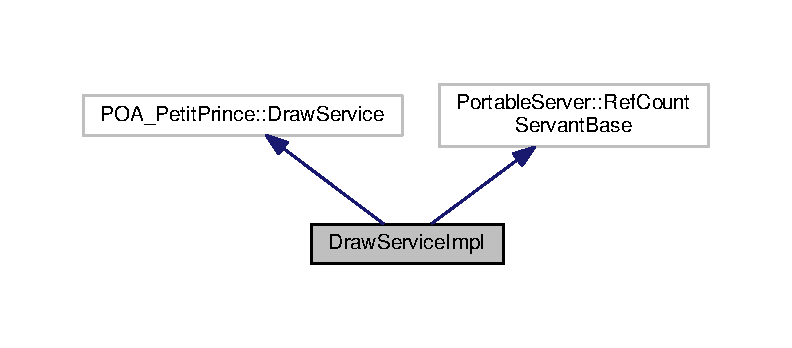
\includegraphics[width=350pt]{class_draw_service_impl__inherit__graph}
\end{center}
\end{figure}


Collaboration diagram for Draw\+Service\+Impl\+:
\nopagebreak
\begin{figure}[H]
\begin{center}
\leavevmode
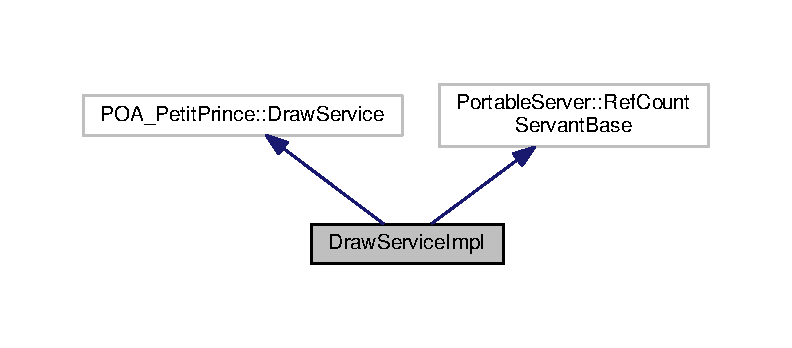
\includegraphics[width=350pt]{class_draw_service_impl__coll__graph}
\end{center}
\end{figure}
\subsection*{Public Member Functions}
\begin{DoxyCompactItemize}
\item 
\hyperlink{class_draw_service_impl_a87d912a8f00ffa723cb8f53431f5266b}{Draw\+Service\+Impl} ()
\item 
\hyperlink{class_draw_service_impl_aba8a8c89630f768c86934aa551bd7632}{Draw\+Service\+Impl} (const \hyperlink{class_draw_service_impl}{Draw\+Service\+Impl} \&orig)
\item 
virtual \hyperlink{class_draw_service_impl_a3531c121d4fafaad26c3768397e9ba80}{$\sim$\+Draw\+Service\+Impl} ()
\item 
\+::C\+O\+R\+B\+A\+::\+Double \hyperlink{class_draw_service_impl_a20bbe30191a183eff973b0d3122f2c8c}{area} (\+::C\+O\+R\+B\+A\+::\+Long id) override
\item 
\+::C\+O\+R\+B\+A\+::\+Double \hyperlink{class_draw_service_impl_a137cc7ebfafc7bb133396a59a47e0cad}{perimeter} (\+::C\+O\+R\+B\+A\+::\+Long id) override
\item 
void \hyperlink{class_draw_service_impl_a2ded991472f1d2e1afab3a475360e070}{homothetie} (\+::C\+O\+R\+B\+A\+::\+Long id,\+::C\+O\+R\+B\+A\+::\+Double index) override
\item 
void \hyperlink{class_draw_service_impl_a0b11a8d94d84c97a00de63873370e932}{translation} (\+::C\+O\+R\+B\+A\+::\+Long id,\+::C\+O\+R\+B\+A\+::\+Double x,\+::C\+O\+R\+B\+A\+::\+Double y) override
\item 
void \hyperlink{class_draw_service_impl_a01fab41862413e70cd171883c36056a7}{rotation} (\+::C\+O\+R\+B\+A\+::\+Long id,\+::C\+O\+R\+B\+A\+::\+Double angle) override
\item 
void \hyperlink{class_draw_service_impl_a6d464f4798e45309ce29c69a60a04d2d}{sym\+Center} (\+::C\+O\+R\+B\+A\+::\+Long id) override
\item 
void \hyperlink{class_draw_service_impl_aa2aa750626c52f3e00056216e854e09e}{sym\+Axial} (\+::C\+O\+R\+B\+A\+::\+Long id) override
\item 
void \hyperlink{class_draw_service_impl_a9e4fe6a245439b112c5985682d759fb2}{add\+Draw} (\+::C\+O\+R\+B\+A\+::\+Long pid,\+::C\+O\+R\+B\+A\+::\+Long cid) override
\item 
char $\ast$ \hyperlink{class_draw_service_impl_ae22a80ed71105e8cca0b664d6f384866}{to\+String} (\+::C\+O\+R\+B\+A\+::\+Long id) override
\end{DoxyCompactItemize}


\subsection{Detailed Description}


Definition at line 20 of file Draw\+Service\+Impl.\+hpp.



\subsection{Constructor \& Destructor Documentation}
\index{Draw\+Service\+Impl@{Draw\+Service\+Impl}!Draw\+Service\+Impl@{Draw\+Service\+Impl}}
\index{Draw\+Service\+Impl@{Draw\+Service\+Impl}!Draw\+Service\+Impl@{Draw\+Service\+Impl}}
\subsubsection[{\texorpdfstring{Draw\+Service\+Impl()}{DrawServiceImpl()}}]{\setlength{\rightskip}{0pt plus 5cm}Draw\+Service\+Impl\+::\+Draw\+Service\+Impl (
\begin{DoxyParamCaption}
{}
\end{DoxyParamCaption}
)}\hypertarget{class_draw_service_impl_a87d912a8f00ffa723cb8f53431f5266b}{}\label{class_draw_service_impl_a87d912a8f00ffa723cb8f53431f5266b}
\index{Draw\+Service\+Impl@{Draw\+Service\+Impl}!Draw\+Service\+Impl@{Draw\+Service\+Impl}}
\index{Draw\+Service\+Impl@{Draw\+Service\+Impl}!Draw\+Service\+Impl@{Draw\+Service\+Impl}}
\subsubsection[{\texorpdfstring{Draw\+Service\+Impl(const Draw\+Service\+Impl \&orig)}{DrawServiceImpl(const DrawServiceImpl &orig)}}]{\setlength{\rightskip}{0pt plus 5cm}Draw\+Service\+Impl\+::\+Draw\+Service\+Impl (
\begin{DoxyParamCaption}
\item[{const {\bf Draw\+Service\+Impl} \&}]{orig}
\end{DoxyParamCaption}
)}\hypertarget{class_draw_service_impl_aba8a8c89630f768c86934aa551bd7632}{}\label{class_draw_service_impl_aba8a8c89630f768c86934aa551bd7632}
\index{Draw\+Service\+Impl@{Draw\+Service\+Impl}!````~Draw\+Service\+Impl@{$\sim$\+Draw\+Service\+Impl}}
\index{````~Draw\+Service\+Impl@{$\sim$\+Draw\+Service\+Impl}!Draw\+Service\+Impl@{Draw\+Service\+Impl}}
\subsubsection[{\texorpdfstring{$\sim$\+Draw\+Service\+Impl()}{~DrawServiceImpl()}}]{\setlength{\rightskip}{0pt plus 5cm}virtual Draw\+Service\+Impl\+::$\sim$\+Draw\+Service\+Impl (
\begin{DoxyParamCaption}
{}
\end{DoxyParamCaption}
)\hspace{0.3cm}{\ttfamily [virtual]}}\hypertarget{class_draw_service_impl_a3531c121d4fafaad26c3768397e9ba80}{}\label{class_draw_service_impl_a3531c121d4fafaad26c3768397e9ba80}


\subsection{Member Function Documentation}
\index{Draw\+Service\+Impl@{Draw\+Service\+Impl}!add\+Draw@{add\+Draw}}
\index{add\+Draw@{add\+Draw}!Draw\+Service\+Impl@{Draw\+Service\+Impl}}
\subsubsection[{\texorpdfstring{add\+Draw(\+::\+C\+O\+R\+B\+A\+::\+Long pid,\+::\+C\+O\+R\+B\+A\+::\+Long cid) override}{addDraw(::CORBA::Long pid,::CORBA::Long cid) override}}]{\setlength{\rightskip}{0pt plus 5cm}void Draw\+Service\+Impl\+::add\+Draw (
\begin{DoxyParamCaption}
\item[{\+::C\+O\+R\+B\+A\+::\+Long}]{pid, }
\item[{\+::C\+O\+R\+B\+A\+::\+Long}]{cid}
\end{DoxyParamCaption}
)\hspace{0.3cm}{\ttfamily [override]}}\hypertarget{class_draw_service_impl_a9e4fe6a245439b112c5985682d759fb2}{}\label{class_draw_service_impl_a9e4fe6a245439b112c5985682d759fb2}
\index{Draw\+Service\+Impl@{Draw\+Service\+Impl}!area@{area}}
\index{area@{area}!Draw\+Service\+Impl@{Draw\+Service\+Impl}}
\subsubsection[{\texorpdfstring{area(\+::\+C\+O\+R\+B\+A\+::\+Long id) override}{area(::CORBA::Long id) override}}]{\setlength{\rightskip}{0pt plus 5cm}\+::C\+O\+R\+B\+A\+::\+Double Draw\+Service\+Impl\+::area (
\begin{DoxyParamCaption}
\item[{\+::C\+O\+R\+B\+A\+::\+Long}]{id}
\end{DoxyParamCaption}
)\hspace{0.3cm}{\ttfamily [override]}}\hypertarget{class_draw_service_impl_a20bbe30191a183eff973b0d3122f2c8c}{}\label{class_draw_service_impl_a20bbe30191a183eff973b0d3122f2c8c}
\index{Draw\+Service\+Impl@{Draw\+Service\+Impl}!homothetie@{homothetie}}
\index{homothetie@{homothetie}!Draw\+Service\+Impl@{Draw\+Service\+Impl}}
\subsubsection[{\texorpdfstring{homothetie(\+::\+C\+O\+R\+B\+A\+::\+Long id,\+::\+C\+O\+R\+B\+A\+::\+Double index) override}{homothetie(::CORBA::Long id,::CORBA::Double index) override}}]{\setlength{\rightskip}{0pt plus 5cm}void Draw\+Service\+Impl\+::homothetie (
\begin{DoxyParamCaption}
\item[{\+::C\+O\+R\+B\+A\+::\+Long}]{id, }
\item[{\+::C\+O\+R\+B\+A\+::\+Double}]{index}
\end{DoxyParamCaption}
)\hspace{0.3cm}{\ttfamily [override]}}\hypertarget{class_draw_service_impl_a2ded991472f1d2e1afab3a475360e070}{}\label{class_draw_service_impl_a2ded991472f1d2e1afab3a475360e070}
\index{Draw\+Service\+Impl@{Draw\+Service\+Impl}!perimeter@{perimeter}}
\index{perimeter@{perimeter}!Draw\+Service\+Impl@{Draw\+Service\+Impl}}
\subsubsection[{\texorpdfstring{perimeter(\+::\+C\+O\+R\+B\+A\+::\+Long id) override}{perimeter(::CORBA::Long id) override}}]{\setlength{\rightskip}{0pt plus 5cm}\+::C\+O\+R\+B\+A\+::\+Double Draw\+Service\+Impl\+::perimeter (
\begin{DoxyParamCaption}
\item[{\+::C\+O\+R\+B\+A\+::\+Long}]{id}
\end{DoxyParamCaption}
)\hspace{0.3cm}{\ttfamily [override]}}\hypertarget{class_draw_service_impl_a137cc7ebfafc7bb133396a59a47e0cad}{}\label{class_draw_service_impl_a137cc7ebfafc7bb133396a59a47e0cad}
\index{Draw\+Service\+Impl@{Draw\+Service\+Impl}!rotation@{rotation}}
\index{rotation@{rotation}!Draw\+Service\+Impl@{Draw\+Service\+Impl}}
\subsubsection[{\texorpdfstring{rotation(\+::\+C\+O\+R\+B\+A\+::\+Long id,\+::\+C\+O\+R\+B\+A\+::\+Double angle) override}{rotation(::CORBA::Long id,::CORBA::Double angle) override}}]{\setlength{\rightskip}{0pt plus 5cm}void Draw\+Service\+Impl\+::rotation (
\begin{DoxyParamCaption}
\item[{\+::C\+O\+R\+B\+A\+::\+Long}]{id, }
\item[{\+::C\+O\+R\+B\+A\+::\+Double}]{angle}
\end{DoxyParamCaption}
)\hspace{0.3cm}{\ttfamily [override]}}\hypertarget{class_draw_service_impl_a01fab41862413e70cd171883c36056a7}{}\label{class_draw_service_impl_a01fab41862413e70cd171883c36056a7}
\index{Draw\+Service\+Impl@{Draw\+Service\+Impl}!sym\+Axial@{sym\+Axial}}
\index{sym\+Axial@{sym\+Axial}!Draw\+Service\+Impl@{Draw\+Service\+Impl}}
\subsubsection[{\texorpdfstring{sym\+Axial(\+::\+C\+O\+R\+B\+A\+::\+Long id) override}{symAxial(::CORBA::Long id) override}}]{\setlength{\rightskip}{0pt plus 5cm}void Draw\+Service\+Impl\+::sym\+Axial (
\begin{DoxyParamCaption}
\item[{\+::C\+O\+R\+B\+A\+::\+Long}]{id}
\end{DoxyParamCaption}
)\hspace{0.3cm}{\ttfamily [override]}}\hypertarget{class_draw_service_impl_aa2aa750626c52f3e00056216e854e09e}{}\label{class_draw_service_impl_aa2aa750626c52f3e00056216e854e09e}
\index{Draw\+Service\+Impl@{Draw\+Service\+Impl}!sym\+Center@{sym\+Center}}
\index{sym\+Center@{sym\+Center}!Draw\+Service\+Impl@{Draw\+Service\+Impl}}
\subsubsection[{\texorpdfstring{sym\+Center(\+::\+C\+O\+R\+B\+A\+::\+Long id) override}{symCenter(::CORBA::Long id) override}}]{\setlength{\rightskip}{0pt plus 5cm}void Draw\+Service\+Impl\+::sym\+Center (
\begin{DoxyParamCaption}
\item[{\+::C\+O\+R\+B\+A\+::\+Long}]{id}
\end{DoxyParamCaption}
)\hspace{0.3cm}{\ttfamily [override]}}\hypertarget{class_draw_service_impl_a6d464f4798e45309ce29c69a60a04d2d}{}\label{class_draw_service_impl_a6d464f4798e45309ce29c69a60a04d2d}
\index{Draw\+Service\+Impl@{Draw\+Service\+Impl}!to\+String@{to\+String}}
\index{to\+String@{to\+String}!Draw\+Service\+Impl@{Draw\+Service\+Impl}}
\subsubsection[{\texorpdfstring{to\+String(\+::\+C\+O\+R\+B\+A\+::\+Long id) override}{toString(::CORBA::Long id) override}}]{\setlength{\rightskip}{0pt plus 5cm}char$\ast$ Draw\+Service\+Impl\+::to\+String (
\begin{DoxyParamCaption}
\item[{\+::C\+O\+R\+B\+A\+::\+Long}]{id}
\end{DoxyParamCaption}
)\hspace{0.3cm}{\ttfamily [override]}}\hypertarget{class_draw_service_impl_ae22a80ed71105e8cca0b664d6f384866}{}\label{class_draw_service_impl_ae22a80ed71105e8cca0b664d6f384866}
\index{Draw\+Service\+Impl@{Draw\+Service\+Impl}!translation@{translation}}
\index{translation@{translation}!Draw\+Service\+Impl@{Draw\+Service\+Impl}}
\subsubsection[{\texorpdfstring{translation(\+::\+C\+O\+R\+B\+A\+::\+Long id,\+::\+C\+O\+R\+B\+A\+::\+Double x,\+::\+C\+O\+R\+B\+A\+::\+Double y) override}{translation(::CORBA::Long id,::CORBA::Double x,::CORBA::Double y) override}}]{\setlength{\rightskip}{0pt plus 5cm}void Draw\+Service\+Impl\+::translation (
\begin{DoxyParamCaption}
\item[{\+::C\+O\+R\+B\+A\+::\+Long}]{id, }
\item[{\+::C\+O\+R\+B\+A\+::\+Double}]{x, }
\item[{\+::C\+O\+R\+B\+A\+::\+Double}]{y}
\end{DoxyParamCaption}
)\hspace{0.3cm}{\ttfamily [override]}}\hypertarget{class_draw_service_impl_a0b11a8d94d84c97a00de63873370e932}{}\label{class_draw_service_impl_a0b11a8d94d84c97a00de63873370e932}


The documentation for this class was generated from the following file\+:\begin{DoxyCompactItemize}
\item 
hdr/\hyperlink{_draw_service_impl_8hpp}{Draw\+Service\+Impl.\+hpp}\end{DoxyCompactItemize}

\hypertarget{class_ellipse}{}\section{Ellipse Class Reference}
\label{class_ellipse}\index{Ellipse@{Ellipse}}


{\ttfamily \#include $<$O\+B\+V\+\_\+\+Ellipse.\+hpp$>$}



Inheritance diagram for Ellipse\+:
\nopagebreak
\begin{figure}[H]
\begin{center}
\leavevmode
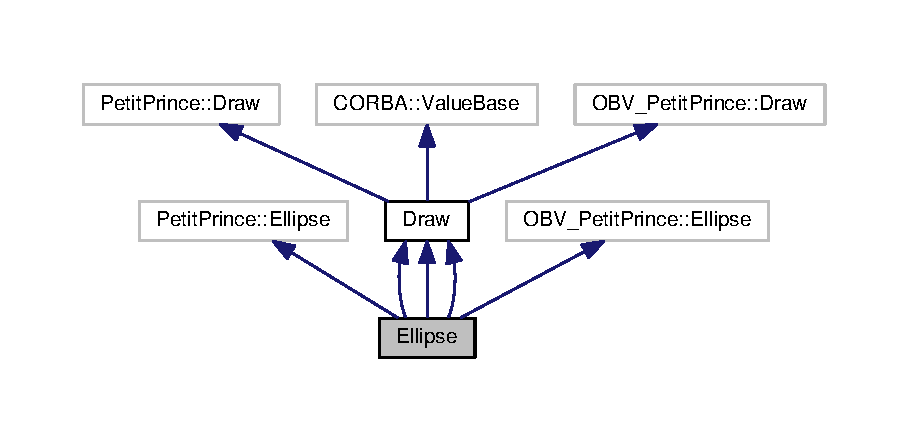
\includegraphics[width=350pt]{class_ellipse__inherit__graph}
\end{center}
\end{figure}


Collaboration diagram for Ellipse\+:
\nopagebreak
\begin{figure}[H]
\begin{center}
\leavevmode
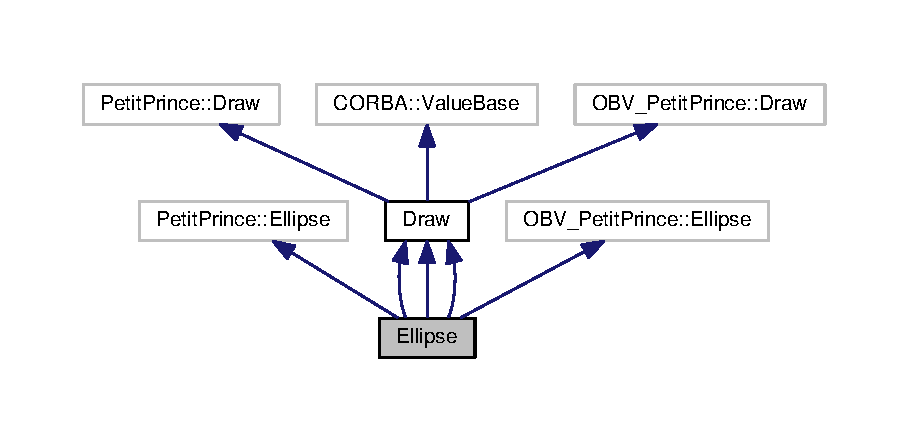
\includegraphics[width=350pt]{class_ellipse__coll__graph}
\end{center}
\end{figure}
\subsection*{Public Types}
\begin{DoxyCompactItemize}
\item 
typedef \hyperlink{class_ellipse}{Ellipse} $\ast$ \hyperlink{class_ellipse_ac03e9a197e4d346d6a7f4360f83affdc}{\+\_\+ptr\+\_\+type}
\item 
typedef \hyperlink{_petit_prince_8hpp_a2e82f3c0eab1432cbb901c90c56b845d}{Ellipse\+\_\+var} \hyperlink{class_ellipse_af5ce6e507c505dcd1b6ef888b904616f}{\+\_\+var\+\_\+type}
\end{DoxyCompactItemize}
\subsection*{Public Member Functions}
\begin{DoxyCompactItemize}
\item 
\hyperlink{class_ellipse_af073bec49d45372f9ed8afd4f22dd528}{Ellipse} (\+::C\+O\+R\+B\+A\+::\+Long \hyperlink{class_draw_a1bf27c5a59da9002d55936c947dce2cc}{id}, char $\ast$\hyperlink{class_draw_a4781c654db63e069c8c5be017f6ccc34}{author},\+::Petit\+Prince\+::\+Point \hyperlink{class_ellipse_ad5e117e2df2c0103e89544e3a051f74d}{center},\+::C\+O\+R\+B\+A\+::\+Double \hyperlink{class_ellipse_a5776141608d4d5bbfaac0f2036bf111a}{long\+\_\+ray},\+::C\+O\+R\+B\+A\+::\+Double \hyperlink{class_ellipse_a955c0a05e02b4bb11df206f08c9c7650}{short\+\_\+ray})
\begin{DoxyCompactList}\small\item\em The public constructor of the class \hyperlink{class_ellipse}{Ellipse}. \end{DoxyCompactList}\item 
virtual \hyperlink{class_ellipse_a5ab8160e6bf40ced81490d6d83d33d89}{$\sim$\+Ellipse} ()
\item 
\+::C\+O\+R\+B\+A\+::\+Double \hyperlink{class_ellipse_a74ed2332ecafb22f8eb2484f85039697}{area} () override
\begin{DoxyCompactList}\small\item\em This method calculate the area of the draw, if applicable. \end{DoxyCompactList}\item 
\+::C\+O\+R\+B\+A\+::\+Double \hyperlink{class_ellipse_a6ac85ef20816de34cf540808dd7fe573}{perimeter} () override
\item 
void \hyperlink{class_ellipse_af73259e055705e0dab10e5671c4031de}{homothetie} (\+::C\+O\+R\+B\+A\+::\+Double indice) override
\begin{DoxyCompactList}\small\item\em This method apply an homothetie to the draw. \end{DoxyCompactList}\item 
void \hyperlink{class_ellipse_ac5d0cb3f7beb9b62688ecf06b8c7f193}{translation} (\+::C\+O\+R\+B\+A\+::\+Double x,\+::C\+O\+R\+B\+A\+::\+Double y) override
\begin{DoxyCompactList}\small\item\em This method apply a translation to the draw. \end{DoxyCompactList}\item 
void \hyperlink{class_ellipse_a58a77992e5d24f53f3011dfb8b08a8e7}{rotation} (\+::C\+O\+R\+B\+A\+::\+Double angle) override
\begin{DoxyCompactList}\small\item\em This method apply a rotation to the draw. \end{DoxyCompactList}\item 
void \hyperlink{class_ellipse_ac78274d703236f85efebd2db6767f640}{sym\+Center} () override
\begin{DoxyCompactList}\small\item\em This method apply a central symetry to the draw. \end{DoxyCompactList}\item 
void \hyperlink{class_ellipse_ad9956caa2504bbb07d4df9493f03d503}{sym\+Axial} () override
\begin{DoxyCompactList}\small\item\em This method apply a axial symetry to the draw. \end{DoxyCompactList}\item 
char $\ast$ \hyperlink{class_ellipse_ad04e67710b8eef3e89e95456ea602479}{to\+String} () override
\begin{DoxyCompactList}\small\item\em Generate a user-\/friendly representation of this draw. \end{DoxyCompactList}\item 
\+::Petit\+Prince\+::\+Point \hyperlink{class_ellipse_ad5e117e2df2c0103e89544e3a051f74d}{center} () override
\item 
void \hyperlink{class_ellipse_aaafe4d4981d9a51f798c8474f8ad42ee}{center} (const \+::Petit\+Prince\+::\+Point \&\+\_\+v) override
\item 
\+::C\+O\+R\+B\+A\+::\+Double \hyperlink{class_ellipse_a5776141608d4d5bbfaac0f2036bf111a}{long\+\_\+ray} () override
\item 
void \hyperlink{class_ellipse_a59dced7606ea1c3d657c7753edfae078}{long\+\_\+ray} (\+::C\+O\+R\+B\+A\+::\+Double \+\_\+v) override
\item 
\+::C\+O\+R\+B\+A\+::\+Double \hyperlink{class_ellipse_a955c0a05e02b4bb11df206f08c9c7650}{short\+\_\+ray} () override
\item 
void \hyperlink{class_ellipse_a626d2025a6e27ec4f52a4f419219a5cd}{short\+\_\+ray} (\+::C\+O\+R\+B\+A\+::\+Double \+\_\+v) override
\item 
virtual \+::C\+O\+R\+B\+A\+::\+Value\+Base $\ast$ \hyperlink{class_ellipse_a325a05f5f1c4141ec6c99e416564b476}{\+\_\+copy\+\_\+value} ()
\item 
virtual \hyperlink{struct_point}{Point} \hyperlink{class_ellipse_a7c167034ea6380590201091da189a08b}{center} ()=0
\item 
virtual void \hyperlink{class_ellipse_a9002930f3e980351e775592942cac3fc}{center} (const \+::Petit\+Prince\+::\+Point \&\+\_\+v)=0
\item 
virtual \+::C\+O\+R\+B\+A\+::\+Double \hyperlink{class_ellipse_a2656a501e4ee8296f8ec71aa5b63f4db}{long\+\_\+ray} ()=0
\item 
virtual void \hyperlink{class_ellipse_ae089aa3f771974912d1c73d9db94cc70}{long\+\_\+ray} (\+::C\+O\+R\+B\+A\+::\+Double \+\_\+v)=0
\item 
virtual \+::C\+O\+R\+B\+A\+::\+Double \hyperlink{class_ellipse_a836989b508beb2da448363e5ed63aec2}{short\+\_\+ray} ()=0
\item 
virtual void \hyperlink{class_ellipse_a4d6bf30278c2839a5d38aa4351cf3a2f}{short\+\_\+ray} (\+::C\+O\+R\+B\+A\+::\+Double \+\_\+v)=0
\item 
virtual const char $\ast$ \hyperlink{class_ellipse_a0e56c51dadf0c21c5f3c82bd7ae3c34c}{\+\_\+\+N\+P\+\_\+repository\+Id} () const 
\item 
virtual const char $\ast$ \hyperlink{class_ellipse_a61c90841d732f4e69247545fc736c321}{\+\_\+\+N\+P\+\_\+repository\+Id} (\+::C\+O\+R\+B\+A\+::\+U\+Long \&\+\_\+hashval) const 
\item 
virtual const \+\_\+omni\+\_\+\+Value\+Ids $\ast$ \hyperlink{class_ellipse_ae5257f936afdfbbeb0ef3344231fc111}{\+\_\+\+N\+P\+\_\+truncatable\+Ids} () const 
\item 
virtual \+::C\+O\+R\+B\+A\+::\+Boolean \hyperlink{class_ellipse_a020acd78a7f680f73c99dd038170749c}{\+\_\+\+N\+P\+\_\+custom} () const 
\item 
virtual void $\ast$ \hyperlink{class_ellipse_a7a69ec5b0954f4c623c9f450afb71d6c}{\+\_\+ptr\+To\+Value} (const char $\ast$\hyperlink{class_draw_a1bf27c5a59da9002d55936c947dce2cc}{id})
\item 
virtual void \hyperlink{class_ellipse_a63076fc769000247bd13c910dbf54c9e}{\+\_\+\+P\+R\+\_\+marshal\+\_\+state} (cdr\+Stream \&) const 
\item 
virtual void \hyperlink{class_ellipse_aa4dea62b56229863d757ae8861c225da}{\+\_\+\+P\+R\+\_\+unmarshal\+\_\+state} (cdr\+Stream \&)
\item 
virtual void \hyperlink{class_ellipse_a9959b5cef873ad4debf7ce4841172522}{\+\_\+\+P\+R\+\_\+copy\+\_\+state} (\hyperlink{class_ellipse}{Ellipse} $\ast$)
\end{DoxyCompactItemize}
\subsection*{Static Public Member Functions}
\begin{DoxyCompactItemize}
\item 
static \hyperlink{class_draw_a5164256572b3c4123ceecd1897c248dd}{\+\_\+ptr\+\_\+type} \hyperlink{class_ellipse_acbcf7089f6cceeee9bb7663221f94cfa}{\+\_\+downcast} (\+::C\+O\+R\+B\+A\+::\+Value\+Base $\ast$)
\item 
static void \hyperlink{class_ellipse_a7b86d2bf246fb67efe6b43220c7509d9}{\+\_\+\+N\+P\+\_\+marshal} (\hyperlink{class_ellipse}{Ellipse} $\ast$, cdr\+Stream \&)
\item 
static \hyperlink{class_ellipse}{Ellipse} $\ast$ \hyperlink{class_ellipse_a1c519c9754fc33d80898ed92b470770a}{\+\_\+\+N\+P\+\_\+unmarshal} (cdr\+Stream \&)
\end{DoxyCompactItemize}
\subsection*{Static Public Attributes}
\begin{DoxyCompactItemize}
\item 
static \hyperlink{_petit_prince_8hpp_a5f7bf7cddb608c2aad7c95f55f8a33c5}{\+\_\+core\+\_\+attr} const char $\ast$ \hyperlink{class_ellipse_a9d889330622bef63cd90c0f42e7ee344}{\+\_\+\+P\+D\+\_\+repo\+Id}
\end{DoxyCompactItemize}
\subsection*{Protected Member Functions}
\begin{DoxyCompactItemize}
\item 
\hyperlink{class_ellipse_aaff4917eddd8882616fe2f956151ba9b}{Ellipse} ()
\item 
virtual \hyperlink{class_ellipse_a5ab8160e6bf40ced81490d6d83d33d89}{$\sim$\+Ellipse} ()
\item 
\hyperlink{class_ellipse_aaff4917eddd8882616fe2f956151ba9b}{Ellipse} ()
\item 
virtual \hyperlink{class_ellipse_a5ab8160e6bf40ced81490d6d83d33d89}{$\sim$\+Ellipse} ()
\end{DoxyCompactItemize}


\subsection{Detailed Description}


Definition at line 24 of file O\+B\+V\+\_\+\+Ellipse.\+hpp.



\subsection{Member Typedef Documentation}
\index{Ellipse@{Ellipse}!\+\_\+ptr\+\_\+type@{\+\_\+ptr\+\_\+type}}
\index{\+\_\+ptr\+\_\+type@{\+\_\+ptr\+\_\+type}!Ellipse@{Ellipse}}
\subsubsection[{\texorpdfstring{\+\_\+ptr\+\_\+type}{_ptr_type}}]{\setlength{\rightskip}{0pt plus 5cm}typedef {\bf Ellipse}$\ast$ {\bf Ellipse\+::\+\_\+ptr\+\_\+type}}\hypertarget{class_ellipse_ac03e9a197e4d346d6a7f4360f83affdc}{}\label{class_ellipse_ac03e9a197e4d346d6a7f4360f83affdc}


Definition at line 611 of file Petit\+Prince.\+hpp.

\index{Ellipse@{Ellipse}!\+\_\+var\+\_\+type@{\+\_\+var\+\_\+type}}
\index{\+\_\+var\+\_\+type@{\+\_\+var\+\_\+type}!Ellipse@{Ellipse}}
\subsubsection[{\texorpdfstring{\+\_\+var\+\_\+type}{_var_type}}]{\setlength{\rightskip}{0pt plus 5cm}typedef {\bf Ellipse\+\_\+var} {\bf Ellipse\+::\+\_\+var\+\_\+type}}\hypertarget{class_ellipse_af5ce6e507c505dcd1b6ef888b904616f}{}\label{class_ellipse_af5ce6e507c505dcd1b6ef888b904616f}


Definition at line 612 of file Petit\+Prince.\+hpp.



\subsection{Constructor \& Destructor Documentation}
\index{Ellipse@{Ellipse}!Ellipse@{Ellipse}}
\index{Ellipse@{Ellipse}!Ellipse@{Ellipse}}
\subsubsection[{\texorpdfstring{Ellipse(\+::\+C\+O\+R\+B\+A\+::\+Long id, char $\ast$author,\+::\+Petit\+Prince\+::\+Point center,\+::\+C\+O\+R\+B\+A\+::\+Double long\+\_\+ray,\+::\+C\+O\+R\+B\+A\+::\+Double short\+\_\+ray)}{Ellipse(::CORBA::Long id, char *author,::PetitPrince::Point center,::CORBA::Double long_ray,::CORBA::Double short_ray)}}]{\setlength{\rightskip}{0pt plus 5cm}Ellipse\+::\+Ellipse (
\begin{DoxyParamCaption}
\item[{\+::C\+O\+R\+B\+A\+::\+Long}]{id, }
\item[{char $\ast$}]{author, }
\item[{\+::Petit\+Prince\+::\+Point}]{center, }
\item[{\+::C\+O\+R\+B\+A\+::\+Double}]{long\+\_\+ray, }
\item[{\+::C\+O\+R\+B\+A\+::\+Double}]{short\+\_\+ray}
\end{DoxyParamCaption}
)\hspace{0.3cm}{\ttfamily [inline]}}\hypertarget{class_ellipse_af073bec49d45372f9ed8afd4f22dd528}{}\label{class_ellipse_af073bec49d45372f9ed8afd4f22dd528}


The public constructor of the class \hyperlink{class_ellipse}{Ellipse}. 


\begin{DoxyParams}{Parameters}
{\em id} & the id of the draw (auto-\/generated) \\
\hline
{\em author} & the author of the draw \\
\hline
{\em center} & the center point for this ellipse \\
\hline
{\em long\+\_\+ray} & the long ray for this ellipse \\
\hline
{\em short\+\_\+ray} & the short ray for this ellipse \\
\hline
\end{DoxyParams}


Definition at line 36 of file O\+B\+V\+\_\+\+Ellipse.\+hpp.

\index{Ellipse@{Ellipse}!````~Ellipse@{$\sim$\+Ellipse}}
\index{````~Ellipse@{$\sim$\+Ellipse}!Ellipse@{Ellipse}}
\subsubsection[{\texorpdfstring{$\sim$\+Ellipse()}{~Ellipse()}}]{\setlength{\rightskip}{0pt plus 5cm}virtual Ellipse\+::$\sim$\+Ellipse (
\begin{DoxyParamCaption}
{}
\end{DoxyParamCaption}
)\hspace{0.3cm}{\ttfamily [inline]}, {\ttfamily [virtual]}}\hypertarget{class_ellipse_a5ab8160e6bf40ced81490d6d83d33d89}{}\label{class_ellipse_a5ab8160e6bf40ced81490d6d83d33d89}


Definition at line 39 of file O\+B\+V\+\_\+\+Ellipse.\+hpp.

\index{Ellipse@{Ellipse}!Ellipse@{Ellipse}}
\index{Ellipse@{Ellipse}!Ellipse@{Ellipse}}
\subsubsection[{\texorpdfstring{Ellipse()}{Ellipse()}}]{\setlength{\rightskip}{0pt plus 5cm}Ellipse\+::\+Ellipse (
\begin{DoxyParamCaption}
{}
\end{DoxyParamCaption}
)\hspace{0.3cm}{\ttfamily [protected]}}\hypertarget{class_ellipse_aaff4917eddd8882616fe2f956151ba9b}{}\label{class_ellipse_aaff4917eddd8882616fe2f956151ba9b}
\index{Ellipse@{Ellipse}!````~Ellipse@{$\sim$\+Ellipse}}
\index{````~Ellipse@{$\sim$\+Ellipse}!Ellipse@{Ellipse}}
\subsubsection[{\texorpdfstring{$\sim$\+Ellipse()}{~Ellipse()}}]{\setlength{\rightskip}{0pt plus 5cm}virtual Ellipse\+::$\sim$\+Ellipse (
\begin{DoxyParamCaption}
{}
\end{DoxyParamCaption}
)\hspace{0.3cm}{\ttfamily [protected]}, {\ttfamily [virtual]}}\hypertarget{class_ellipse_a5ab8160e6bf40ced81490d6d83d33d89}{}\label{class_ellipse_a5ab8160e6bf40ced81490d6d83d33d89}
\index{Ellipse@{Ellipse}!Ellipse@{Ellipse}}
\index{Ellipse@{Ellipse}!Ellipse@{Ellipse}}
\subsubsection[{\texorpdfstring{Ellipse()}{Ellipse()}}]{\setlength{\rightskip}{0pt plus 5cm}Ellipse\+::\+Ellipse (
\begin{DoxyParamCaption}
{}
\end{DoxyParamCaption}
)\hspace{0.3cm}{\ttfamily [protected]}}\hypertarget{class_ellipse_aaff4917eddd8882616fe2f956151ba9b}{}\label{class_ellipse_aaff4917eddd8882616fe2f956151ba9b}
\index{Ellipse@{Ellipse}!````~Ellipse@{$\sim$\+Ellipse}}
\index{````~Ellipse@{$\sim$\+Ellipse}!Ellipse@{Ellipse}}
\subsubsection[{\texorpdfstring{$\sim$\+Ellipse()}{~Ellipse()}}]{\setlength{\rightskip}{0pt plus 5cm}virtual Ellipse\+::$\sim$\+Ellipse (
\begin{DoxyParamCaption}
{}
\end{DoxyParamCaption}
)\hspace{0.3cm}{\ttfamily [protected]}, {\ttfamily [virtual]}}\hypertarget{class_ellipse_a5ab8160e6bf40ced81490d6d83d33d89}{}\label{class_ellipse_a5ab8160e6bf40ced81490d6d83d33d89}


\subsection{Member Function Documentation}
\index{Ellipse@{Ellipse}!\+\_\+copy\+\_\+value@{\+\_\+copy\+\_\+value}}
\index{\+\_\+copy\+\_\+value@{\+\_\+copy\+\_\+value}!Ellipse@{Ellipse}}
\subsubsection[{\texorpdfstring{\+\_\+copy\+\_\+value()}{_copy_value()}}]{\setlength{\rightskip}{0pt plus 5cm}virtual \+::C\+O\+R\+B\+A\+::\+Value\+Base$\ast$ Ellipse\+::\+\_\+copy\+\_\+value (
\begin{DoxyParamCaption}
{}
\end{DoxyParamCaption}
)}\hypertarget{class_ellipse_a325a05f5f1c4141ec6c99e416564b476}{}\label{class_ellipse_a325a05f5f1c4141ec6c99e416564b476}
\index{Ellipse@{Ellipse}!\+\_\+downcast@{\+\_\+downcast}}
\index{\+\_\+downcast@{\+\_\+downcast}!Ellipse@{Ellipse}}
\subsubsection[{\texorpdfstring{\+\_\+downcast(\+::\+C\+O\+R\+B\+A\+::\+Value\+Base $\ast$)}{_downcast(::CORBA::ValueBase *)}}]{\setlength{\rightskip}{0pt plus 5cm}static {\bf \+\_\+ptr\+\_\+type} Ellipse\+::\+\_\+downcast (
\begin{DoxyParamCaption}
\item[{\+::C\+O\+R\+B\+A\+::\+Value\+Base $\ast$}]{}
\end{DoxyParamCaption}
)\hspace{0.3cm}{\ttfamily [static]}}\hypertarget{class_ellipse_acbcf7089f6cceeee9bb7663221f94cfa}{}\label{class_ellipse_acbcf7089f6cceeee9bb7663221f94cfa}
\index{Ellipse@{Ellipse}!\+\_\+\+N\+P\+\_\+custom@{\+\_\+\+N\+P\+\_\+custom}}
\index{\+\_\+\+N\+P\+\_\+custom@{\+\_\+\+N\+P\+\_\+custom}!Ellipse@{Ellipse}}
\subsubsection[{\texorpdfstring{\+\_\+\+N\+P\+\_\+custom() const }{_NP_custom() const }}]{\setlength{\rightskip}{0pt plus 5cm}virtual \+::C\+O\+R\+B\+A\+::\+Boolean Ellipse\+::\+\_\+\+N\+P\+\_\+custom (
\begin{DoxyParamCaption}
{}
\end{DoxyParamCaption}
) const}\hypertarget{class_ellipse_a020acd78a7f680f73c99dd038170749c}{}\label{class_ellipse_a020acd78a7f680f73c99dd038170749c}
\index{Ellipse@{Ellipse}!\+\_\+\+N\+P\+\_\+marshal@{\+\_\+\+N\+P\+\_\+marshal}}
\index{\+\_\+\+N\+P\+\_\+marshal@{\+\_\+\+N\+P\+\_\+marshal}!Ellipse@{Ellipse}}
\subsubsection[{\texorpdfstring{\+\_\+\+N\+P\+\_\+marshal(\+Ellipse $\ast$, cdr\+Stream \&)}{_NP_marshal(Ellipse *, cdrStream &)}}]{\setlength{\rightskip}{0pt plus 5cm}static void Ellipse\+::\+\_\+\+N\+P\+\_\+marshal (
\begin{DoxyParamCaption}
\item[{{\bf Ellipse} $\ast$}]{, }
\item[{cdr\+Stream \&}]{}
\end{DoxyParamCaption}
)\hspace{0.3cm}{\ttfamily [static]}}\hypertarget{class_ellipse_a7b86d2bf246fb67efe6b43220c7509d9}{}\label{class_ellipse_a7b86d2bf246fb67efe6b43220c7509d9}
\index{Ellipse@{Ellipse}!\+\_\+\+N\+P\+\_\+repository\+Id@{\+\_\+\+N\+P\+\_\+repository\+Id}}
\index{\+\_\+\+N\+P\+\_\+repository\+Id@{\+\_\+\+N\+P\+\_\+repository\+Id}!Ellipse@{Ellipse}}
\subsubsection[{\texorpdfstring{\+\_\+\+N\+P\+\_\+repository\+Id() const }{_NP_repositoryId() const }}]{\setlength{\rightskip}{0pt plus 5cm}virtual const char$\ast$ Ellipse\+::\+\_\+\+N\+P\+\_\+repository\+Id (
\begin{DoxyParamCaption}
{}
\end{DoxyParamCaption}
) const\hspace{0.3cm}{\ttfamily [virtual]}}\hypertarget{class_ellipse_a0e56c51dadf0c21c5f3c82bd7ae3c34c}{}\label{class_ellipse_a0e56c51dadf0c21c5f3c82bd7ae3c34c}


Reimplemented from \hyperlink{class_draw_a90d2c0a9b6aed68ca30ea2a7187317dc}{Draw}.

\index{Ellipse@{Ellipse}!\+\_\+\+N\+P\+\_\+repository\+Id@{\+\_\+\+N\+P\+\_\+repository\+Id}}
\index{\+\_\+\+N\+P\+\_\+repository\+Id@{\+\_\+\+N\+P\+\_\+repository\+Id}!Ellipse@{Ellipse}}
\subsubsection[{\texorpdfstring{\+\_\+\+N\+P\+\_\+repository\+Id(\+::\+C\+O\+R\+B\+A\+::\+U\+Long \&\+\_\+hashval) const }{_NP_repositoryId(::CORBA::ULong &_hashval) const }}]{\setlength{\rightskip}{0pt plus 5cm}virtual const char$\ast$ Ellipse\+::\+\_\+\+N\+P\+\_\+repository\+Id (
\begin{DoxyParamCaption}
\item[{\+::C\+O\+R\+B\+A\+::\+U\+Long \&}]{\+\_\+hashval}
\end{DoxyParamCaption}
) const\hspace{0.3cm}{\ttfamily [virtual]}}\hypertarget{class_ellipse_a61c90841d732f4e69247545fc736c321}{}\label{class_ellipse_a61c90841d732f4e69247545fc736c321}


Reimplemented from \hyperlink{class_draw_ae24df04b0f119c2fb6fd525a041f081d}{Draw}.

\index{Ellipse@{Ellipse}!\+\_\+\+N\+P\+\_\+truncatable\+Ids@{\+\_\+\+N\+P\+\_\+truncatable\+Ids}}
\index{\+\_\+\+N\+P\+\_\+truncatable\+Ids@{\+\_\+\+N\+P\+\_\+truncatable\+Ids}!Ellipse@{Ellipse}}
\subsubsection[{\texorpdfstring{\+\_\+\+N\+P\+\_\+truncatable\+Ids() const }{_NP_truncatableIds() const }}]{\setlength{\rightskip}{0pt plus 5cm}virtual const \+\_\+omni\+\_\+\+Value\+Ids$\ast$ Ellipse\+::\+\_\+\+N\+P\+\_\+truncatable\+Ids (
\begin{DoxyParamCaption}
{}
\end{DoxyParamCaption}
) const\hspace{0.3cm}{\ttfamily [virtual]}}\hypertarget{class_ellipse_ae5257f936afdfbbeb0ef3344231fc111}{}\label{class_ellipse_ae5257f936afdfbbeb0ef3344231fc111}


Reimplemented from \hyperlink{class_draw_a10a319bcb2ef5d6ac5439859fe9f126e}{Draw}.

\index{Ellipse@{Ellipse}!\+\_\+\+N\+P\+\_\+unmarshal@{\+\_\+\+N\+P\+\_\+unmarshal}}
\index{\+\_\+\+N\+P\+\_\+unmarshal@{\+\_\+\+N\+P\+\_\+unmarshal}!Ellipse@{Ellipse}}
\subsubsection[{\texorpdfstring{\+\_\+\+N\+P\+\_\+unmarshal(cdr\+Stream \&)}{_NP_unmarshal(cdrStream &)}}]{\setlength{\rightskip}{0pt plus 5cm}static {\bf Ellipse}$\ast$ Ellipse\+::\+\_\+\+N\+P\+\_\+unmarshal (
\begin{DoxyParamCaption}
\item[{cdr\+Stream \&}]{}
\end{DoxyParamCaption}
)\hspace{0.3cm}{\ttfamily [static]}}\hypertarget{class_ellipse_a1c519c9754fc33d80898ed92b470770a}{}\label{class_ellipse_a1c519c9754fc33d80898ed92b470770a}
\index{Ellipse@{Ellipse}!\+\_\+\+P\+R\+\_\+copy\+\_\+state@{\+\_\+\+P\+R\+\_\+copy\+\_\+state}}
\index{\+\_\+\+P\+R\+\_\+copy\+\_\+state@{\+\_\+\+P\+R\+\_\+copy\+\_\+state}!Ellipse@{Ellipse}}
\subsubsection[{\texorpdfstring{\+\_\+\+P\+R\+\_\+copy\+\_\+state(\+Ellipse $\ast$)}{_PR_copy_state(Ellipse *)}}]{\setlength{\rightskip}{0pt plus 5cm}virtual void Ellipse\+::\+\_\+\+P\+R\+\_\+copy\+\_\+state (
\begin{DoxyParamCaption}
\item[{{\bf Ellipse} $\ast$}]{}
\end{DoxyParamCaption}
)\hspace{0.3cm}{\ttfamily [virtual]}}\hypertarget{class_ellipse_a9959b5cef873ad4debf7ce4841172522}{}\label{class_ellipse_a9959b5cef873ad4debf7ce4841172522}
\index{Ellipse@{Ellipse}!\+\_\+\+P\+R\+\_\+marshal\+\_\+state@{\+\_\+\+P\+R\+\_\+marshal\+\_\+state}}
\index{\+\_\+\+P\+R\+\_\+marshal\+\_\+state@{\+\_\+\+P\+R\+\_\+marshal\+\_\+state}!Ellipse@{Ellipse}}
\subsubsection[{\texorpdfstring{\+\_\+\+P\+R\+\_\+marshal\+\_\+state(cdr\+Stream \&) const }{_PR_marshal_state(cdrStream &) const }}]{\setlength{\rightskip}{0pt plus 5cm}virtual void Ellipse\+::\+\_\+\+P\+R\+\_\+marshal\+\_\+state (
\begin{DoxyParamCaption}
\item[{cdr\+Stream \&}]{}
\end{DoxyParamCaption}
) const\hspace{0.3cm}{\ttfamily [virtual]}}\hypertarget{class_ellipse_a63076fc769000247bd13c910dbf54c9e}{}\label{class_ellipse_a63076fc769000247bd13c910dbf54c9e}


Reimplemented from \hyperlink{class_draw_adfa1e0ac94bad822e332caeddc17f02a}{Draw}.

\index{Ellipse@{Ellipse}!\+\_\+\+P\+R\+\_\+unmarshal\+\_\+state@{\+\_\+\+P\+R\+\_\+unmarshal\+\_\+state}}
\index{\+\_\+\+P\+R\+\_\+unmarshal\+\_\+state@{\+\_\+\+P\+R\+\_\+unmarshal\+\_\+state}!Ellipse@{Ellipse}}
\subsubsection[{\texorpdfstring{\+\_\+\+P\+R\+\_\+unmarshal\+\_\+state(cdr\+Stream \&)}{_PR_unmarshal_state(cdrStream &)}}]{\setlength{\rightskip}{0pt plus 5cm}virtual void Ellipse\+::\+\_\+\+P\+R\+\_\+unmarshal\+\_\+state (
\begin{DoxyParamCaption}
\item[{cdr\+Stream \&}]{}
\end{DoxyParamCaption}
)\hspace{0.3cm}{\ttfamily [virtual]}}\hypertarget{class_ellipse_aa4dea62b56229863d757ae8861c225da}{}\label{class_ellipse_aa4dea62b56229863d757ae8861c225da}


Reimplemented from \hyperlink{class_draw_a62dc59ec12f9ebd4da1f3448dbec683f}{Draw}.

\index{Ellipse@{Ellipse}!\+\_\+ptr\+To\+Value@{\+\_\+ptr\+To\+Value}}
\index{\+\_\+ptr\+To\+Value@{\+\_\+ptr\+To\+Value}!Ellipse@{Ellipse}}
\subsubsection[{\texorpdfstring{\+\_\+ptr\+To\+Value(const char $\ast$id)}{_ptrToValue(const char *id)}}]{\setlength{\rightskip}{0pt plus 5cm}virtual void$\ast$ Ellipse\+::\+\_\+ptr\+To\+Value (
\begin{DoxyParamCaption}
\item[{const char $\ast$}]{id}
\end{DoxyParamCaption}
)\hspace{0.3cm}{\ttfamily [virtual]}}\hypertarget{class_ellipse_a7a69ec5b0954f4c623c9f450afb71d6c}{}\label{class_ellipse_a7a69ec5b0954f4c623c9f450afb71d6c}


Reimplemented from \hyperlink{class_draw_a2924173c6238dd077531f555324155b9}{Draw}.

\index{Ellipse@{Ellipse}!area@{area}}
\index{area@{area}!Ellipse@{Ellipse}}
\subsubsection[{\texorpdfstring{area() override}{area() override}}]{\setlength{\rightskip}{0pt plus 5cm}C\+O\+R\+B\+A\+::\+Double Ellipse\+::area (
\begin{DoxyParamCaption}
{}
\end{DoxyParamCaption}
)\hspace{0.3cm}{\ttfamily [inline]}, {\ttfamily [override]}, {\ttfamily [virtual]}}\hypertarget{class_ellipse_a74ed2332ecafb22f8eb2484f85039697}{}\label{class_ellipse_a74ed2332ecafb22f8eb2484f85039697}


This method calculate the area of the draw, if applicable. 

\begin{DoxyReturn}{Returns}
the area of this draw 
\end{DoxyReturn}


Implements \hyperlink{class_draw_a0fb84e185ec13237aa456962d1eb0816}{Draw}.



Definition at line 50 of file O\+B\+V\+\_\+\+Ellipse.\+hpp.

\index{Ellipse@{Ellipse}!center@{center}}
\index{center@{center}!Ellipse@{Ellipse}}
\subsubsection[{\texorpdfstring{center() override}{center() override}}]{\setlength{\rightskip}{0pt plus 5cm}\+::Petit\+Prince\+::\+Point Ellipse\+::center (
\begin{DoxyParamCaption}
{}
\end{DoxyParamCaption}
)\hspace{0.3cm}{\ttfamily [inline]}, {\ttfamily [override]}}\hypertarget{class_ellipse_ad5e117e2df2c0103e89544e3a051f74d}{}\label{class_ellipse_ad5e117e2df2c0103e89544e3a051f74d}


Definition at line 129 of file O\+B\+V\+\_\+\+Ellipse.\+hpp.

\index{Ellipse@{Ellipse}!center@{center}}
\index{center@{center}!Ellipse@{Ellipse}}
\subsubsection[{\texorpdfstring{center(const \+::\+Petit\+Prince\+::\+Point \&\+\_\+v) override}{center(const ::PetitPrince::Point &_v) override}}]{\setlength{\rightskip}{0pt plus 5cm}void Ellipse\+::center (
\begin{DoxyParamCaption}
\item[{const \+::Petit\+Prince\+::\+Point \&}]{\+\_\+v}
\end{DoxyParamCaption}
)\hspace{0.3cm}{\ttfamily [inline]}, {\ttfamily [override]}}\hypertarget{class_ellipse_aaafe4d4981d9a51f798c8474f8ad42ee}{}\label{class_ellipse_aaafe4d4981d9a51f798c8474f8ad42ee}


Definition at line 139 of file O\+B\+V\+\_\+\+Ellipse.\+hpp.

\index{Ellipse@{Ellipse}!center@{center}}
\index{center@{center}!Ellipse@{Ellipse}}
\subsubsection[{\texorpdfstring{center()=0}{center()=0}}]{\setlength{\rightskip}{0pt plus 5cm}virtual {\bf Point} Ellipse\+::center (
\begin{DoxyParamCaption}
{}
\end{DoxyParamCaption}
)\hspace{0.3cm}{\ttfamily [pure virtual]}}\hypertarget{class_ellipse_a7c167034ea6380590201091da189a08b}{}\label{class_ellipse_a7c167034ea6380590201091da189a08b}
\index{Ellipse@{Ellipse}!center@{center}}
\index{center@{center}!Ellipse@{Ellipse}}
\subsubsection[{\texorpdfstring{center(const \+::\+Petit\+Prince\+::\+Point \&\+\_\+v)=0}{center(const ::PetitPrince::Point &_v)=0}}]{\setlength{\rightskip}{0pt plus 5cm}virtual void Ellipse\+::center (
\begin{DoxyParamCaption}
\item[{const \+::Petit\+Prince\+::\+Point \&}]{\+\_\+v}
\end{DoxyParamCaption}
)\hspace{0.3cm}{\ttfamily [pure virtual]}}\hypertarget{class_ellipse_a9002930f3e980351e775592942cac3fc}{}\label{class_ellipse_a9002930f3e980351e775592942cac3fc}
\index{Ellipse@{Ellipse}!homothetie@{homothetie}}
\index{homothetie@{homothetie}!Ellipse@{Ellipse}}
\subsubsection[{\texorpdfstring{homothetie(\+::\+C\+O\+R\+B\+A\+::\+Double indice) override}{homothetie(::CORBA::Double indice) override}}]{\setlength{\rightskip}{0pt plus 5cm}void Ellipse\+::homothetie (
\begin{DoxyParamCaption}
\item[{\+::C\+O\+R\+B\+A\+::\+Double}]{indice}
\end{DoxyParamCaption}
)\hspace{0.3cm}{\ttfamily [inline]}, {\ttfamily [override]}, {\ttfamily [virtual]}}\hypertarget{class_ellipse_af73259e055705e0dab10e5671c4031de}{}\label{class_ellipse_af73259e055705e0dab10e5671c4031de}


This method apply an homothetie to the draw. 


\begin{DoxyParams}{Parameters}
{\em indice} & the scalar factor defining the homothetie. \\
\hline
\end{DoxyParams}


Implements \hyperlink{class_draw_a39387bf248da4d7d91bee9099d4b6fca}{Draw}.



Definition at line 70 of file O\+B\+V\+\_\+\+Ellipse.\+hpp.

\index{Ellipse@{Ellipse}!long\+\_\+ray@{long\+\_\+ray}}
\index{long\+\_\+ray@{long\+\_\+ray}!Ellipse@{Ellipse}}
\subsubsection[{\texorpdfstring{long\+\_\+ray() override}{long_ray() override}}]{\setlength{\rightskip}{0pt plus 5cm}\+::C\+O\+R\+B\+A\+::\+Double Ellipse\+::long\+\_\+ray (
\begin{DoxyParamCaption}
{}
\end{DoxyParamCaption}
)\hspace{0.3cm}{\ttfamily [inline]}, {\ttfamily [override]}}\hypertarget{class_ellipse_a5776141608d4d5bbfaac0f2036bf111a}{}\label{class_ellipse_a5776141608d4d5bbfaac0f2036bf111a}


Definition at line 149 of file O\+B\+V\+\_\+\+Ellipse.\+hpp.

\index{Ellipse@{Ellipse}!long\+\_\+ray@{long\+\_\+ray}}
\index{long\+\_\+ray@{long\+\_\+ray}!Ellipse@{Ellipse}}
\subsubsection[{\texorpdfstring{long\+\_\+ray(\+::\+C\+O\+R\+B\+A\+::\+Double \+\_\+v) override}{long_ray(::CORBA::Double _v) override}}]{\setlength{\rightskip}{0pt plus 5cm}void Ellipse\+::long\+\_\+ray (
\begin{DoxyParamCaption}
\item[{\+::C\+O\+R\+B\+A\+::\+Double}]{\+\_\+v}
\end{DoxyParamCaption}
)\hspace{0.3cm}{\ttfamily [inline]}, {\ttfamily [override]}}\hypertarget{class_ellipse_a59dced7606ea1c3d657c7753edfae078}{}\label{class_ellipse_a59dced7606ea1c3d657c7753edfae078}


Definition at line 159 of file O\+B\+V\+\_\+\+Ellipse.\+hpp.

\index{Ellipse@{Ellipse}!long\+\_\+ray@{long\+\_\+ray}}
\index{long\+\_\+ray@{long\+\_\+ray}!Ellipse@{Ellipse}}
\subsubsection[{\texorpdfstring{long\+\_\+ray()=0}{long_ray()=0}}]{\setlength{\rightskip}{0pt plus 5cm}virtual \+::C\+O\+R\+B\+A\+::\+Double Ellipse\+::long\+\_\+ray (
\begin{DoxyParamCaption}
{}
\end{DoxyParamCaption}
)\hspace{0.3cm}{\ttfamily [pure virtual]}}\hypertarget{class_ellipse_a2656a501e4ee8296f8ec71aa5b63f4db}{}\label{class_ellipse_a2656a501e4ee8296f8ec71aa5b63f4db}
\index{Ellipse@{Ellipse}!long\+\_\+ray@{long\+\_\+ray}}
\index{long\+\_\+ray@{long\+\_\+ray}!Ellipse@{Ellipse}}
\subsubsection[{\texorpdfstring{long\+\_\+ray(\+::\+C\+O\+R\+B\+A\+::\+Double \+\_\+v)=0}{long_ray(::CORBA::Double _v)=0}}]{\setlength{\rightskip}{0pt plus 5cm}virtual void Ellipse\+::long\+\_\+ray (
\begin{DoxyParamCaption}
\item[{\+::C\+O\+R\+B\+A\+::\+Double}]{\+\_\+v}
\end{DoxyParamCaption}
)\hspace{0.3cm}{\ttfamily [pure virtual]}}\hypertarget{class_ellipse_ae089aa3f771974912d1c73d9db94cc70}{}\label{class_ellipse_ae089aa3f771974912d1c73d9db94cc70}
\index{Ellipse@{Ellipse}!perimeter@{perimeter}}
\index{perimeter@{perimeter}!Ellipse@{Ellipse}}
\subsubsection[{\texorpdfstring{perimeter() override}{perimeter() override}}]{\setlength{\rightskip}{0pt plus 5cm}\+::C\+O\+R\+B\+A\+::\+Double Ellipse\+::perimeter (
\begin{DoxyParamCaption}
{}
\end{DoxyParamCaption}
)\hspace{0.3cm}{\ttfamily [inline]}, {\ttfamily [override]}, {\ttfamily [virtual]}}\hypertarget{class_ellipse_a6ac85ef20816de34cf540808dd7fe573}{}\label{class_ellipse_a6ac85ef20816de34cf540808dd7fe573}


Implements \hyperlink{class_draw_a7171f2b64135c81a41cb5a7a9926af52}{Draw}.



Definition at line 60 of file O\+B\+V\+\_\+\+Ellipse.\+hpp.

\index{Ellipse@{Ellipse}!rotation@{rotation}}
\index{rotation@{rotation}!Ellipse@{Ellipse}}
\subsubsection[{\texorpdfstring{rotation(\+::\+C\+O\+R\+B\+A\+::\+Double angle) override}{rotation(::CORBA::Double angle) override}}]{\setlength{\rightskip}{0pt plus 5cm}void Ellipse\+::rotation (
\begin{DoxyParamCaption}
\item[{\+::C\+O\+R\+B\+A\+::\+Double}]{angle}
\end{DoxyParamCaption}
)\hspace{0.3cm}{\ttfamily [inline]}, {\ttfamily [override]}, {\ttfamily [virtual]}}\hypertarget{class_ellipse_a58a77992e5d24f53f3011dfb8b08a8e7}{}\label{class_ellipse_a58a77992e5d24f53f3011dfb8b08a8e7}


This method apply a rotation to the draw. 


\begin{DoxyParams}{Parameters}
{\em angle} & the angle defining the rotation. \\
\hline
\end{DoxyParams}


Implements \hyperlink{class_draw_ab45c311ee0963a1a5e3ba3ac461e467c}{Draw}.



Definition at line 93 of file O\+B\+V\+\_\+\+Ellipse.\+hpp.

\index{Ellipse@{Ellipse}!short\+\_\+ray@{short\+\_\+ray}}
\index{short\+\_\+ray@{short\+\_\+ray}!Ellipse@{Ellipse}}
\subsubsection[{\texorpdfstring{short\+\_\+ray() override}{short_ray() override}}]{\setlength{\rightskip}{0pt plus 5cm}\+::C\+O\+R\+B\+A\+::\+Double Ellipse\+::short\+\_\+ray (
\begin{DoxyParamCaption}
{}
\end{DoxyParamCaption}
)\hspace{0.3cm}{\ttfamily [inline]}, {\ttfamily [override]}}\hypertarget{class_ellipse_a955c0a05e02b4bb11df206f08c9c7650}{}\label{class_ellipse_a955c0a05e02b4bb11df206f08c9c7650}


Definition at line 169 of file O\+B\+V\+\_\+\+Ellipse.\+hpp.

\index{Ellipse@{Ellipse}!short\+\_\+ray@{short\+\_\+ray}}
\index{short\+\_\+ray@{short\+\_\+ray}!Ellipse@{Ellipse}}
\subsubsection[{\texorpdfstring{short\+\_\+ray(\+::\+C\+O\+R\+B\+A\+::\+Double \+\_\+v) override}{short_ray(::CORBA::Double _v) override}}]{\setlength{\rightskip}{0pt plus 5cm}void Ellipse\+::short\+\_\+ray (
\begin{DoxyParamCaption}
\item[{\+::C\+O\+R\+B\+A\+::\+Double}]{\+\_\+v}
\end{DoxyParamCaption}
)\hspace{0.3cm}{\ttfamily [inline]}, {\ttfamily [override]}}\hypertarget{class_ellipse_a626d2025a6e27ec4f52a4f419219a5cd}{}\label{class_ellipse_a626d2025a6e27ec4f52a4f419219a5cd}


Definition at line 179 of file O\+B\+V\+\_\+\+Ellipse.\+hpp.

\index{Ellipse@{Ellipse}!short\+\_\+ray@{short\+\_\+ray}}
\index{short\+\_\+ray@{short\+\_\+ray}!Ellipse@{Ellipse}}
\subsubsection[{\texorpdfstring{short\+\_\+ray()=0}{short_ray()=0}}]{\setlength{\rightskip}{0pt plus 5cm}virtual \+::C\+O\+R\+B\+A\+::\+Double Ellipse\+::short\+\_\+ray (
\begin{DoxyParamCaption}
{}
\end{DoxyParamCaption}
)\hspace{0.3cm}{\ttfamily [pure virtual]}}\hypertarget{class_ellipse_a836989b508beb2da448363e5ed63aec2}{}\label{class_ellipse_a836989b508beb2da448363e5ed63aec2}
\index{Ellipse@{Ellipse}!short\+\_\+ray@{short\+\_\+ray}}
\index{short\+\_\+ray@{short\+\_\+ray}!Ellipse@{Ellipse}}
\subsubsection[{\texorpdfstring{short\+\_\+ray(\+::\+C\+O\+R\+B\+A\+::\+Double \+\_\+v)=0}{short_ray(::CORBA::Double _v)=0}}]{\setlength{\rightskip}{0pt plus 5cm}virtual void Ellipse\+::short\+\_\+ray (
\begin{DoxyParamCaption}
\item[{\+::C\+O\+R\+B\+A\+::\+Double}]{\+\_\+v}
\end{DoxyParamCaption}
)\hspace{0.3cm}{\ttfamily [pure virtual]}}\hypertarget{class_ellipse_a4d6bf30278c2839a5d38aa4351cf3a2f}{}\label{class_ellipse_a4d6bf30278c2839a5d38aa4351cf3a2f}
\index{Ellipse@{Ellipse}!sym\+Axial@{sym\+Axial}}
\index{sym\+Axial@{sym\+Axial}!Ellipse@{Ellipse}}
\subsubsection[{\texorpdfstring{sym\+Axial() override}{symAxial() override}}]{\setlength{\rightskip}{0pt plus 5cm}void Ellipse\+::sym\+Axial (
\begin{DoxyParamCaption}
{}
\end{DoxyParamCaption}
)\hspace{0.3cm}{\ttfamily [inline]}, {\ttfamily [override]}, {\ttfamily [virtual]}}\hypertarget{class_ellipse_ad9956caa2504bbb07d4df9493f03d503}{}\label{class_ellipse_ad9956caa2504bbb07d4df9493f03d503}


This method apply a axial symetry to the draw. 



Implements \hyperlink{class_draw_aede358197311244da0fe937fb7e9573e}{Draw}.



Definition at line 107 of file O\+B\+V\+\_\+\+Ellipse.\+hpp.

\index{Ellipse@{Ellipse}!sym\+Center@{sym\+Center}}
\index{sym\+Center@{sym\+Center}!Ellipse@{Ellipse}}
\subsubsection[{\texorpdfstring{sym\+Center() override}{symCenter() override}}]{\setlength{\rightskip}{0pt plus 5cm}void Ellipse\+::sym\+Center (
\begin{DoxyParamCaption}
{}
\end{DoxyParamCaption}
)\hspace{0.3cm}{\ttfamily [inline]}, {\ttfamily [override]}, {\ttfamily [virtual]}}\hypertarget{class_ellipse_ac78274d703236f85efebd2db6767f640}{}\label{class_ellipse_ac78274d703236f85efebd2db6767f640}


This method apply a central symetry to the draw. 



Implements \hyperlink{class_draw_a1a10bbbeb1ccd4b10b04226f3fe10755}{Draw}.



Definition at line 100 of file O\+B\+V\+\_\+\+Ellipse.\+hpp.

\index{Ellipse@{Ellipse}!to\+String@{to\+String}}
\index{to\+String@{to\+String}!Ellipse@{Ellipse}}
\subsubsection[{\texorpdfstring{to\+String() override}{toString() override}}]{\setlength{\rightskip}{0pt plus 5cm}char $\ast$ Ellipse\+::to\+String (
\begin{DoxyParamCaption}
{}
\end{DoxyParamCaption}
)\hspace{0.3cm}{\ttfamily [inline]}, {\ttfamily [override]}, {\ttfamily [virtual]}}\hypertarget{class_ellipse_ad04e67710b8eef3e89e95456ea602479}{}\label{class_ellipse_ad04e67710b8eef3e89e95456ea602479}


Generate a user-\/friendly representation of this draw. 

\begin{DoxyReturn}{Returns}
The user-\/friendly representation of this draw 
\end{DoxyReturn}


Implements \hyperlink{class_draw_a0dd9c8b5127149b28e54bd602c797cca}{Draw}.



Definition at line 116 of file O\+B\+V\+\_\+\+Ellipse.\+hpp.

\index{Ellipse@{Ellipse}!translation@{translation}}
\index{translation@{translation}!Ellipse@{Ellipse}}
\subsubsection[{\texorpdfstring{translation(\+::\+C\+O\+R\+B\+A\+::\+Double x,\+::\+C\+O\+R\+B\+A\+::\+Double y) override}{translation(::CORBA::Double x,::CORBA::Double y) override}}]{\setlength{\rightskip}{0pt plus 5cm}void Ellipse\+::translation (
\begin{DoxyParamCaption}
\item[{\+::C\+O\+R\+B\+A\+::\+Double}]{x, }
\item[{\+::C\+O\+R\+B\+A\+::\+Double}]{y}
\end{DoxyParamCaption}
)\hspace{0.3cm}{\ttfamily [inline]}, {\ttfamily [override]}, {\ttfamily [virtual]}}\hypertarget{class_ellipse_ac5d0cb3f7beb9b62688ecf06b8c7f193}{}\label{class_ellipse_ac5d0cb3f7beb9b62688ecf06b8c7f193}


This method apply a translation to the draw. 


\begin{DoxyParams}{Parameters}
{\em x} & the x-\/axis translation \\
\hline
{\em y} & the y-\/axis translation \\
\hline
\end{DoxyParams}


Implements \hyperlink{class_draw_a71e63b40c9505098652a94e06872fdc6}{Draw}.



Definition at line 82 of file O\+B\+V\+\_\+\+Ellipse.\+hpp.



\subsection{Member Data Documentation}
\index{Ellipse@{Ellipse}!\+\_\+\+P\+D\+\_\+repo\+Id@{\+\_\+\+P\+D\+\_\+repo\+Id}}
\index{\+\_\+\+P\+D\+\_\+repo\+Id@{\+\_\+\+P\+D\+\_\+repo\+Id}!Ellipse@{Ellipse}}
\subsubsection[{\texorpdfstring{\+\_\+\+P\+D\+\_\+repo\+Id}{_PD_repoId}}]{\setlength{\rightskip}{0pt plus 5cm}{\bf \+\_\+core\+\_\+attr} const char$\ast$ Ellipse\+::\+\_\+\+P\+D\+\_\+repo\+Id\hspace{0.3cm}{\ttfamily [static]}}\hypertarget{class_ellipse_a9d889330622bef63cd90c0f42e7ee344}{}\label{class_ellipse_a9d889330622bef63cd90c0f42e7ee344}


Definition at line 660 of file Petit\+Prince.\+hpp.



The documentation for this class was generated from the following files\+:\begin{DoxyCompactItemize}
\item 
hdr/\hyperlink{_o_b_v___ellipse_8hpp}{O\+B\+V\+\_\+\+Ellipse.\+hpp}\item 
hdr/\hyperlink{_petit_prince_8hpp}{Petit\+Prince.\+hpp}\end{DoxyCompactItemize}

\hypertarget{class_ellipse___helper}{}\section{Ellipse\+\_\+\+Helper Class Reference}
\label{class_ellipse___helper}\index{Ellipse\+\_\+\+Helper@{Ellipse\+\_\+\+Helper}}


{\ttfamily \#include $<$Petit\+Prince.\+hpp$>$}

\subsection*{Static Public Member Functions}
\begin{DoxyCompactItemize}
\item 
static void \hyperlink{class_ellipse___helper_a116883c1b7635997ada46010938de20d}{add\+\_\+ref} (\hyperlink{class_ellipse}{Ellipse} $\ast$)
\item 
static void \hyperlink{class_ellipse___helper_a7a5442216cc36952d90679a135be68f0}{remove\+\_\+ref} (\hyperlink{class_ellipse}{Ellipse} $\ast$)
\item 
static void \hyperlink{class_ellipse___helper_a33a2f550545232be68768b4c52eda630}{marshal} (\hyperlink{class_ellipse}{Ellipse} $\ast$, cdr\+Stream \&)
\item 
static \hyperlink{class_ellipse}{Ellipse} $\ast$ \hyperlink{class_ellipse___helper_ad86a74c7fbadee3325a822434a5f6d3c}{unmarshal} (cdr\+Stream \&)
\end{DoxyCompactItemize}


\subsection{Detailed Description}


Definition at line 592 of file Petit\+Prince.\+hpp.



\subsection{Member Function Documentation}
\index{Ellipse\+\_\+\+Helper@{Ellipse\+\_\+\+Helper}!add\+\_\+ref@{add\+\_\+ref}}
\index{add\+\_\+ref@{add\+\_\+ref}!Ellipse\+\_\+\+Helper@{Ellipse\+\_\+\+Helper}}
\subsubsection[{\texorpdfstring{add\+\_\+ref(\+Ellipse $\ast$)}{add_ref(Ellipse *)}}]{\setlength{\rightskip}{0pt plus 5cm}static void Ellipse\+\_\+\+Helper\+::add\+\_\+ref (
\begin{DoxyParamCaption}
\item[{{\bf Ellipse} $\ast$}]{}
\end{DoxyParamCaption}
)\hspace{0.3cm}{\ttfamily [static]}}\hypertarget{class_ellipse___helper_a116883c1b7635997ada46010938de20d}{}\label{class_ellipse___helper_a116883c1b7635997ada46010938de20d}
\index{Ellipse\+\_\+\+Helper@{Ellipse\+\_\+\+Helper}!marshal@{marshal}}
\index{marshal@{marshal}!Ellipse\+\_\+\+Helper@{Ellipse\+\_\+\+Helper}}
\subsubsection[{\texorpdfstring{marshal(\+Ellipse $\ast$, cdr\+Stream \&)}{marshal(Ellipse *, cdrStream &)}}]{\setlength{\rightskip}{0pt plus 5cm}static void Ellipse\+\_\+\+Helper\+::marshal (
\begin{DoxyParamCaption}
\item[{{\bf Ellipse} $\ast$}]{, }
\item[{cdr\+Stream \&}]{}
\end{DoxyParamCaption}
)\hspace{0.3cm}{\ttfamily [static]}}\hypertarget{class_ellipse___helper_a33a2f550545232be68768b4c52eda630}{}\label{class_ellipse___helper_a33a2f550545232be68768b4c52eda630}
\index{Ellipse\+\_\+\+Helper@{Ellipse\+\_\+\+Helper}!remove\+\_\+ref@{remove\+\_\+ref}}
\index{remove\+\_\+ref@{remove\+\_\+ref}!Ellipse\+\_\+\+Helper@{Ellipse\+\_\+\+Helper}}
\subsubsection[{\texorpdfstring{remove\+\_\+ref(\+Ellipse $\ast$)}{remove_ref(Ellipse *)}}]{\setlength{\rightskip}{0pt plus 5cm}static void Ellipse\+\_\+\+Helper\+::remove\+\_\+ref (
\begin{DoxyParamCaption}
\item[{{\bf Ellipse} $\ast$}]{}
\end{DoxyParamCaption}
)\hspace{0.3cm}{\ttfamily [static]}}\hypertarget{class_ellipse___helper_a7a5442216cc36952d90679a135be68f0}{}\label{class_ellipse___helper_a7a5442216cc36952d90679a135be68f0}
\index{Ellipse\+\_\+\+Helper@{Ellipse\+\_\+\+Helper}!unmarshal@{unmarshal}}
\index{unmarshal@{unmarshal}!Ellipse\+\_\+\+Helper@{Ellipse\+\_\+\+Helper}}
\subsubsection[{\texorpdfstring{unmarshal(cdr\+Stream \&)}{unmarshal(cdrStream &)}}]{\setlength{\rightskip}{0pt plus 5cm}static {\bf Ellipse}$\ast$ Ellipse\+\_\+\+Helper\+::unmarshal (
\begin{DoxyParamCaption}
\item[{cdr\+Stream \&}]{}
\end{DoxyParamCaption}
)\hspace{0.3cm}{\ttfamily [static]}}\hypertarget{class_ellipse___helper_ad86a74c7fbadee3325a822434a5f6d3c}{}\label{class_ellipse___helper_ad86a74c7fbadee3325a822434a5f6d3c}


The documentation for this class was generated from the following file\+:\begin{DoxyCompactItemize}
\item 
hdr/\hyperlink{_petit_prince_8hpp}{Petit\+Prince.\+hpp}\end{DoxyCompactItemize}

\hypertarget{class_petit_prince_service_1_1_invalid_draw_params}{}\section{Petit\+Prince\+Service\+:\+:Invalid\+Draw\+Params Class Reference}
\label{class_petit_prince_service_1_1_invalid_draw_params}\index{Petit\+Prince\+Service\+::\+Invalid\+Draw\+Params@{Petit\+Prince\+Service\+::\+Invalid\+Draw\+Params}}


{\ttfamily \#include $<$Petit\+Prince.\+hpp$>$}



Inheritance diagram for Petit\+Prince\+Service\+:\+:Invalid\+Draw\+Params\+:
\nopagebreak
\begin{figure}[H]
\begin{center}
\leavevmode
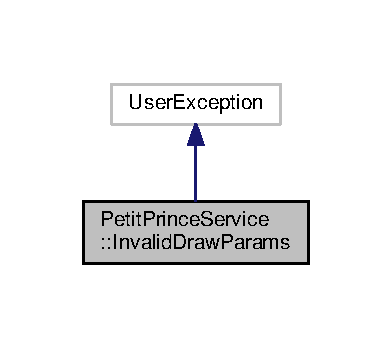
\includegraphics[width=188pt]{class_petit_prince_service_1_1_invalid_draw_params__inherit__graph}
\end{center}
\end{figure}


Collaboration diagram for Petit\+Prince\+Service\+:\+:Invalid\+Draw\+Params\+:
\nopagebreak
\begin{figure}[H]
\begin{center}
\leavevmode
\includegraphics[width=188pt]{class_petit_prince_service_1_1_invalid_draw_params__coll__graph}
\end{center}
\end{figure}
\subsection*{Public Member Functions}
\begin{DoxyCompactItemize}
\item 
\hyperlink{class_petit_prince_service_1_1_invalid_draw_params_ada9c3a277688d5c7e36f59a59697dec2}{Invalid\+Draw\+Params} ()
\item 
\hyperlink{class_petit_prince_service_1_1_invalid_draw_params_ab8e4567f0909cc24064da6227a36c6b3}{Invalid\+Draw\+Params} (const \hyperlink{class_petit_prince_service_1_1_invalid_draw_params}{Invalid\+Draw\+Params} \&)
\item 
\hyperlink{class_petit_prince_service_1_1_invalid_draw_params_a8e422ba4cb343620321e31c1e83d5845}{Invalid\+Draw\+Params} (const char $\ast$i\+\_\+msg)
\item 
\hyperlink{class_petit_prince_service_1_1_invalid_draw_params}{Invalid\+Draw\+Params} \& \hyperlink{class_petit_prince_service_1_1_invalid_draw_params_a04fe5e64e5b7dcc9595b51a3df80a9bb}{operator=} (const \hyperlink{class_petit_prince_service_1_1_invalid_draw_params}{Invalid\+Draw\+Params} \&)
\item 
virtual \hyperlink{class_petit_prince_service_1_1_invalid_draw_params_a3488986314279cc4f5d4f96bad9ecbb0}{$\sim$\+Invalid\+Draw\+Params} ()
\item 
virtual void \hyperlink{class_petit_prince_service_1_1_invalid_draw_params_a6ba6781a38912e9509b28bd7acb14693}{\+\_\+raise} () const 
\item 
void \hyperlink{class_petit_prince_service_1_1_invalid_draw_params_a285adf31166b13ad5fe5587b903b135c}{operator$>$$>$=} (cdr\+Stream \&) const 
\item 
void \hyperlink{class_petit_prince_service_1_1_invalid_draw_params_a064cd2058013b1af2385a932d73849bd}{operator$<$$<$=} (cdr\+Stream \&)
\item 
virtual \+::C\+O\+R\+B\+A\+::\+Exception $\ast$ \hyperlink{class_petit_prince_service_1_1_invalid_draw_params_a6c2845831c714db13d15ee27bfcbf4e2}{\+\_\+\+N\+P\+\_\+duplicate} () const 
\end{DoxyCompactItemize}
\subsection*{Static Public Member Functions}
\begin{DoxyCompactItemize}
\item 
static \hyperlink{class_petit_prince_service_1_1_invalid_draw_params}{Invalid\+Draw\+Params} $\ast$ \hyperlink{class_petit_prince_service_1_1_invalid_draw_params_a4b8271e0145b2887842d8f89a92b3357}{\+\_\+downcast} (\+::C\+O\+R\+B\+A\+::\+Exception $\ast$)
\item 
static const \hyperlink{class_petit_prince_service_1_1_invalid_draw_params}{Invalid\+Draw\+Params} $\ast$ \hyperlink{class_petit_prince_service_1_1_invalid_draw_params_a67da7dcd2127f8c7fa4e915582173d8f}{\+\_\+downcast} (const \+::C\+O\+R\+B\+A\+::\+Exception $\ast$)
\item 
static \hyperlink{class_petit_prince_service_1_1_invalid_draw_params}{Invalid\+Draw\+Params} $\ast$ \hyperlink{class_petit_prince_service_1_1_invalid_draw_params_ad3b94cdc567af14f86cbfccb5ad4a9b4}{\+\_\+narrow} (\+::C\+O\+R\+B\+A\+::\+Exception $\ast$\+\_\+e)
\end{DoxyCompactItemize}
\subsection*{Public Attributes}
\begin{DoxyCompactItemize}
\item 
\+::C\+O\+R\+B\+A\+::\+String\+\_\+member \hyperlink{class_petit_prince_service_1_1_invalid_draw_params_ad20b320baca257a2276e76a6efc94a91}{msg}
\end{DoxyCompactItemize}
\subsection*{Static Public Attributes}
\begin{DoxyCompactItemize}
\item 
static \hyperlink{_petit_prince_8hpp_a5f7bf7cddb608c2aad7c95f55f8a33c5}{\+\_\+core\+\_\+attr} insert\+Exception\+To\+Any \hyperlink{class_petit_prince_service_1_1_invalid_draw_params_a3c0d3050311043226e9d0a0882d4c25f}{insert\+To\+Any\+Fn}
\item 
static \hyperlink{_petit_prince_8hpp_a5f7bf7cddb608c2aad7c95f55f8a33c5}{\+\_\+core\+\_\+attr} insert\+Exception\+To\+Any\+N\+CP \hyperlink{class_petit_prince_service_1_1_invalid_draw_params_afce432eda8989d47faee11da1a73348e}{insert\+To\+Any\+Fn\+N\+CP}
\item 
static \hyperlink{_petit_prince_8hpp_a5f7bf7cddb608c2aad7c95f55f8a33c5}{\+\_\+core\+\_\+attr} const char $\ast$ \hyperlink{class_petit_prince_service_1_1_invalid_draw_params_a74f67513423e12f170c20552e3286cf1}{\+\_\+\+P\+D\+\_\+repo\+Id}
\item 
static \hyperlink{_petit_prince_8hpp_a5f7bf7cddb608c2aad7c95f55f8a33c5}{\+\_\+core\+\_\+attr} const char $\ast$ \hyperlink{class_petit_prince_service_1_1_invalid_draw_params_abd336eae5a88a48f0b2ae8dac1c8fb57}{\+\_\+\+P\+D\+\_\+type\+Id}
\end{DoxyCompactItemize}


\subsection{Detailed Description}


Definition at line 1128 of file Petit\+Prince.\+hpp.



\subsection{Constructor \& Destructor Documentation}
\index{Petit\+Prince\+Service\+::\+Invalid\+Draw\+Params@{Petit\+Prince\+Service\+::\+Invalid\+Draw\+Params}!Invalid\+Draw\+Params@{Invalid\+Draw\+Params}}
\index{Invalid\+Draw\+Params@{Invalid\+Draw\+Params}!Petit\+Prince\+Service\+::\+Invalid\+Draw\+Params@{Petit\+Prince\+Service\+::\+Invalid\+Draw\+Params}}
\subsubsection[{\texorpdfstring{Invalid\+Draw\+Params()}{InvalidDrawParams()}}]{\setlength{\rightskip}{0pt plus 5cm}Petit\+Prince\+Service\+::\+Invalid\+Draw\+Params\+::\+Invalid\+Draw\+Params (
\begin{DoxyParamCaption}
{}
\end{DoxyParamCaption}
)\hspace{0.3cm}{\ttfamily [inline]}}\hypertarget{class_petit_prince_service_1_1_invalid_draw_params_ada9c3a277688d5c7e36f59a59697dec2}{}\label{class_petit_prince_service_1_1_invalid_draw_params_ada9c3a277688d5c7e36f59a59697dec2}


Definition at line 1135 of file Petit\+Prince.\+hpp.

\index{Petit\+Prince\+Service\+::\+Invalid\+Draw\+Params@{Petit\+Prince\+Service\+::\+Invalid\+Draw\+Params}!Invalid\+Draw\+Params@{Invalid\+Draw\+Params}}
\index{Invalid\+Draw\+Params@{Invalid\+Draw\+Params}!Petit\+Prince\+Service\+::\+Invalid\+Draw\+Params@{Petit\+Prince\+Service\+::\+Invalid\+Draw\+Params}}
\subsubsection[{\texorpdfstring{Invalid\+Draw\+Params(const Invalid\+Draw\+Params \&)}{InvalidDrawParams(const InvalidDrawParams &)}}]{\setlength{\rightskip}{0pt plus 5cm}Petit\+Prince\+Service\+::\+Invalid\+Draw\+Params\+::\+Invalid\+Draw\+Params (
\begin{DoxyParamCaption}
\item[{const {\bf Invalid\+Draw\+Params} \&}]{}
\end{DoxyParamCaption}
)}\hypertarget{class_petit_prince_service_1_1_invalid_draw_params_ab8e4567f0909cc24064da6227a36c6b3}{}\label{class_petit_prince_service_1_1_invalid_draw_params_ab8e4567f0909cc24064da6227a36c6b3}
\index{Petit\+Prince\+Service\+::\+Invalid\+Draw\+Params@{Petit\+Prince\+Service\+::\+Invalid\+Draw\+Params}!Invalid\+Draw\+Params@{Invalid\+Draw\+Params}}
\index{Invalid\+Draw\+Params@{Invalid\+Draw\+Params}!Petit\+Prince\+Service\+::\+Invalid\+Draw\+Params@{Petit\+Prince\+Service\+::\+Invalid\+Draw\+Params}}
\subsubsection[{\texorpdfstring{Invalid\+Draw\+Params(const char $\ast$i\+\_\+msg)}{InvalidDrawParams(const char *i_msg)}}]{\setlength{\rightskip}{0pt plus 5cm}Petit\+Prince\+Service\+::\+Invalid\+Draw\+Params\+::\+Invalid\+Draw\+Params (
\begin{DoxyParamCaption}
\item[{const char $\ast$}]{i\+\_\+msg}
\end{DoxyParamCaption}
)}\hypertarget{class_petit_prince_service_1_1_invalid_draw_params_a8e422ba4cb343620321e31c1e83d5845}{}\label{class_petit_prince_service_1_1_invalid_draw_params_a8e422ba4cb343620321e31c1e83d5845}
\index{Petit\+Prince\+Service\+::\+Invalid\+Draw\+Params@{Petit\+Prince\+Service\+::\+Invalid\+Draw\+Params}!````~Invalid\+Draw\+Params@{$\sim$\+Invalid\+Draw\+Params}}
\index{````~Invalid\+Draw\+Params@{$\sim$\+Invalid\+Draw\+Params}!Petit\+Prince\+Service\+::\+Invalid\+Draw\+Params@{Petit\+Prince\+Service\+::\+Invalid\+Draw\+Params}}
\subsubsection[{\texorpdfstring{$\sim$\+Invalid\+Draw\+Params()}{~InvalidDrawParams()}}]{\setlength{\rightskip}{0pt plus 5cm}virtual Petit\+Prince\+Service\+::\+Invalid\+Draw\+Params\+::$\sim$\+Invalid\+Draw\+Params (
\begin{DoxyParamCaption}
{}
\end{DoxyParamCaption}
)\hspace{0.3cm}{\ttfamily [virtual]}}\hypertarget{class_petit_prince_service_1_1_invalid_draw_params_a3488986314279cc4f5d4f96bad9ecbb0}{}\label{class_petit_prince_service_1_1_invalid_draw_params_a3488986314279cc4f5d4f96bad9ecbb0}


\subsection{Member Function Documentation}
\index{Petit\+Prince\+Service\+::\+Invalid\+Draw\+Params@{Petit\+Prince\+Service\+::\+Invalid\+Draw\+Params}!\+\_\+downcast@{\+\_\+downcast}}
\index{\+\_\+downcast@{\+\_\+downcast}!Petit\+Prince\+Service\+::\+Invalid\+Draw\+Params@{Petit\+Prince\+Service\+::\+Invalid\+Draw\+Params}}
\subsubsection[{\texorpdfstring{\+\_\+downcast(\+::\+C\+O\+R\+B\+A\+::\+Exception $\ast$)}{_downcast(::CORBA::Exception *)}}]{\setlength{\rightskip}{0pt plus 5cm}static {\bf Invalid\+Draw\+Params}$\ast$ Petit\+Prince\+Service\+::\+Invalid\+Draw\+Params\+::\+\_\+downcast (
\begin{DoxyParamCaption}
\item[{\+::C\+O\+R\+B\+A\+::\+Exception $\ast$}]{}
\end{DoxyParamCaption}
)\hspace{0.3cm}{\ttfamily [static]}}\hypertarget{class_petit_prince_service_1_1_invalid_draw_params_a4b8271e0145b2887842d8f89a92b3357}{}\label{class_petit_prince_service_1_1_invalid_draw_params_a4b8271e0145b2887842d8f89a92b3357}
\index{Petit\+Prince\+Service\+::\+Invalid\+Draw\+Params@{Petit\+Prince\+Service\+::\+Invalid\+Draw\+Params}!\+\_\+downcast@{\+\_\+downcast}}
\index{\+\_\+downcast@{\+\_\+downcast}!Petit\+Prince\+Service\+::\+Invalid\+Draw\+Params@{Petit\+Prince\+Service\+::\+Invalid\+Draw\+Params}}
\subsubsection[{\texorpdfstring{\+\_\+downcast(const \+::\+C\+O\+R\+B\+A\+::\+Exception $\ast$)}{_downcast(const ::CORBA::Exception *)}}]{\setlength{\rightskip}{0pt plus 5cm}static const {\bf Invalid\+Draw\+Params}$\ast$ Petit\+Prince\+Service\+::\+Invalid\+Draw\+Params\+::\+\_\+downcast (
\begin{DoxyParamCaption}
\item[{const \+::C\+O\+R\+B\+A\+::\+Exception $\ast$}]{}
\end{DoxyParamCaption}
)\hspace{0.3cm}{\ttfamily [static]}}\hypertarget{class_petit_prince_service_1_1_invalid_draw_params_a67da7dcd2127f8c7fa4e915582173d8f}{}\label{class_petit_prince_service_1_1_invalid_draw_params_a67da7dcd2127f8c7fa4e915582173d8f}
\index{Petit\+Prince\+Service\+::\+Invalid\+Draw\+Params@{Petit\+Prince\+Service\+::\+Invalid\+Draw\+Params}!\+\_\+narrow@{\+\_\+narrow}}
\index{\+\_\+narrow@{\+\_\+narrow}!Petit\+Prince\+Service\+::\+Invalid\+Draw\+Params@{Petit\+Prince\+Service\+::\+Invalid\+Draw\+Params}}
\subsubsection[{\texorpdfstring{\+\_\+narrow(\+::\+C\+O\+R\+B\+A\+::\+Exception $\ast$\+\_\+e)}{_narrow(::CORBA::Exception *_e)}}]{\setlength{\rightskip}{0pt plus 5cm}static {\bf Invalid\+Draw\+Params}$\ast$ Petit\+Prince\+Service\+::\+Invalid\+Draw\+Params\+::\+\_\+narrow (
\begin{DoxyParamCaption}
\item[{\+::C\+O\+R\+B\+A\+::\+Exception $\ast$}]{\+\_\+e}
\end{DoxyParamCaption}
)\hspace{0.3cm}{\ttfamily [inline]}, {\ttfamily [static]}}\hypertarget{class_petit_prince_service_1_1_invalid_draw_params_ad3b94cdc567af14f86cbfccb5ad4a9b4}{}\label{class_petit_prince_service_1_1_invalid_draw_params_ad3b94cdc567af14f86cbfccb5ad4a9b4}


Definition at line 1146 of file Petit\+Prince.\+hpp.

\index{Petit\+Prince\+Service\+::\+Invalid\+Draw\+Params@{Petit\+Prince\+Service\+::\+Invalid\+Draw\+Params}!\+\_\+\+N\+P\+\_\+duplicate@{\+\_\+\+N\+P\+\_\+duplicate}}
\index{\+\_\+\+N\+P\+\_\+duplicate@{\+\_\+\+N\+P\+\_\+duplicate}!Petit\+Prince\+Service\+::\+Invalid\+Draw\+Params@{Petit\+Prince\+Service\+::\+Invalid\+Draw\+Params}}
\subsubsection[{\texorpdfstring{\+\_\+\+N\+P\+\_\+duplicate() const }{_NP_duplicate() const }}]{\setlength{\rightskip}{0pt plus 5cm}virtual \+::C\+O\+R\+B\+A\+::\+Exception$\ast$ Petit\+Prince\+Service\+::\+Invalid\+Draw\+Params\+::\+\_\+\+N\+P\+\_\+duplicate (
\begin{DoxyParamCaption}
{}
\end{DoxyParamCaption}
) const}\hypertarget{class_petit_prince_service_1_1_invalid_draw_params_a6c2845831c714db13d15ee27bfcbf4e2}{}\label{class_petit_prince_service_1_1_invalid_draw_params_a6c2845831c714db13d15ee27bfcbf4e2}
\index{Petit\+Prince\+Service\+::\+Invalid\+Draw\+Params@{Petit\+Prince\+Service\+::\+Invalid\+Draw\+Params}!\+\_\+raise@{\+\_\+raise}}
\index{\+\_\+raise@{\+\_\+raise}!Petit\+Prince\+Service\+::\+Invalid\+Draw\+Params@{Petit\+Prince\+Service\+::\+Invalid\+Draw\+Params}}
\subsubsection[{\texorpdfstring{\+\_\+raise() const }{_raise() const }}]{\setlength{\rightskip}{0pt plus 5cm}virtual void Petit\+Prince\+Service\+::\+Invalid\+Draw\+Params\+::\+\_\+raise (
\begin{DoxyParamCaption}
{}
\end{DoxyParamCaption}
) const\hspace{0.3cm}{\ttfamily [virtual]}}\hypertarget{class_petit_prince_service_1_1_invalid_draw_params_a6ba6781a38912e9509b28bd7acb14693}{}\label{class_petit_prince_service_1_1_invalid_draw_params_a6ba6781a38912e9509b28bd7acb14693}
\index{Petit\+Prince\+Service\+::\+Invalid\+Draw\+Params@{Petit\+Prince\+Service\+::\+Invalid\+Draw\+Params}!operator$<$$<$=@{operator$<$$<$=}}
\index{operator$<$$<$=@{operator$<$$<$=}!Petit\+Prince\+Service\+::\+Invalid\+Draw\+Params@{Petit\+Prince\+Service\+::\+Invalid\+Draw\+Params}}
\subsubsection[{\texorpdfstring{operator$<$$<$=(cdr\+Stream \&)}{operator<<=(cdrStream &)}}]{\setlength{\rightskip}{0pt plus 5cm}void Petit\+Prince\+Service\+::\+Invalid\+Draw\+Params\+::operator$<$$<$= (
\begin{DoxyParamCaption}
\item[{cdr\+Stream \&}]{}
\end{DoxyParamCaption}
)}\hypertarget{class_petit_prince_service_1_1_invalid_draw_params_a064cd2058013b1af2385a932d73849bd}{}\label{class_petit_prince_service_1_1_invalid_draw_params_a064cd2058013b1af2385a932d73849bd}
\index{Petit\+Prince\+Service\+::\+Invalid\+Draw\+Params@{Petit\+Prince\+Service\+::\+Invalid\+Draw\+Params}!operator=@{operator=}}
\index{operator=@{operator=}!Petit\+Prince\+Service\+::\+Invalid\+Draw\+Params@{Petit\+Prince\+Service\+::\+Invalid\+Draw\+Params}}
\subsubsection[{\texorpdfstring{operator=(const Invalid\+Draw\+Params \&)}{operator=(const InvalidDrawParams &)}}]{\setlength{\rightskip}{0pt plus 5cm}{\bf Invalid\+Draw\+Params}\& Petit\+Prince\+Service\+::\+Invalid\+Draw\+Params\+::operator= (
\begin{DoxyParamCaption}
\item[{const {\bf Invalid\+Draw\+Params} \&}]{}
\end{DoxyParamCaption}
)}\hypertarget{class_petit_prince_service_1_1_invalid_draw_params_a04fe5e64e5b7dcc9595b51a3df80a9bb}{}\label{class_petit_prince_service_1_1_invalid_draw_params_a04fe5e64e5b7dcc9595b51a3df80a9bb}
\index{Petit\+Prince\+Service\+::\+Invalid\+Draw\+Params@{Petit\+Prince\+Service\+::\+Invalid\+Draw\+Params}!operator$>$$>$=@{operator$>$$>$=}}
\index{operator$>$$>$=@{operator$>$$>$=}!Petit\+Prince\+Service\+::\+Invalid\+Draw\+Params@{Petit\+Prince\+Service\+::\+Invalid\+Draw\+Params}}
\subsubsection[{\texorpdfstring{operator$>$$>$=(cdr\+Stream \&) const }{operator>>=(cdrStream &) const }}]{\setlength{\rightskip}{0pt plus 5cm}void Petit\+Prince\+Service\+::\+Invalid\+Draw\+Params\+::operator$>$$>$= (
\begin{DoxyParamCaption}
\item[{cdr\+Stream \&}]{}
\end{DoxyParamCaption}
) const}\hypertarget{class_petit_prince_service_1_1_invalid_draw_params_a285adf31166b13ad5fe5587b903b135c}{}\label{class_petit_prince_service_1_1_invalid_draw_params_a285adf31166b13ad5fe5587b903b135c}


\subsection{Member Data Documentation}
\index{Petit\+Prince\+Service\+::\+Invalid\+Draw\+Params@{Petit\+Prince\+Service\+::\+Invalid\+Draw\+Params}!\+\_\+\+P\+D\+\_\+repo\+Id@{\+\_\+\+P\+D\+\_\+repo\+Id}}
\index{\+\_\+\+P\+D\+\_\+repo\+Id@{\+\_\+\+P\+D\+\_\+repo\+Id}!Petit\+Prince\+Service\+::\+Invalid\+Draw\+Params@{Petit\+Prince\+Service\+::\+Invalid\+Draw\+Params}}
\subsubsection[{\texorpdfstring{\+\_\+\+P\+D\+\_\+repo\+Id}{_PD_repoId}}]{\setlength{\rightskip}{0pt plus 5cm}{\bf \+\_\+core\+\_\+attr} const char$\ast$ Petit\+Prince\+Service\+::\+Invalid\+Draw\+Params\+::\+\_\+\+P\+D\+\_\+repo\+Id\hspace{0.3cm}{\ttfamily [static]}}\hypertarget{class_petit_prince_service_1_1_invalid_draw_params_a74f67513423e12f170c20552e3286cf1}{}\label{class_petit_prince_service_1_1_invalid_draw_params_a74f67513423e12f170c20552e3286cf1}


Definition at line 1158 of file Petit\+Prince.\+hpp.

\index{Petit\+Prince\+Service\+::\+Invalid\+Draw\+Params@{Petit\+Prince\+Service\+::\+Invalid\+Draw\+Params}!\+\_\+\+P\+D\+\_\+type\+Id@{\+\_\+\+P\+D\+\_\+type\+Id}}
\index{\+\_\+\+P\+D\+\_\+type\+Id@{\+\_\+\+P\+D\+\_\+type\+Id}!Petit\+Prince\+Service\+::\+Invalid\+Draw\+Params@{Petit\+Prince\+Service\+::\+Invalid\+Draw\+Params}}
\subsubsection[{\texorpdfstring{\+\_\+\+P\+D\+\_\+type\+Id}{_PD_typeId}}]{\setlength{\rightskip}{0pt plus 5cm}{\bf \+\_\+core\+\_\+attr} const char$\ast$ Petit\+Prince\+Service\+::\+Invalid\+Draw\+Params\+::\+\_\+\+P\+D\+\_\+type\+Id\hspace{0.3cm}{\ttfamily [static]}}\hypertarget{class_petit_prince_service_1_1_invalid_draw_params_abd336eae5a88a48f0b2ae8dac1c8fb57}{}\label{class_petit_prince_service_1_1_invalid_draw_params_abd336eae5a88a48f0b2ae8dac1c8fb57}


Definition at line 1159 of file Petit\+Prince.\+hpp.

\index{Petit\+Prince\+Service\+::\+Invalid\+Draw\+Params@{Petit\+Prince\+Service\+::\+Invalid\+Draw\+Params}!insert\+To\+Any\+Fn@{insert\+To\+Any\+Fn}}
\index{insert\+To\+Any\+Fn@{insert\+To\+Any\+Fn}!Petit\+Prince\+Service\+::\+Invalid\+Draw\+Params@{Petit\+Prince\+Service\+::\+Invalid\+Draw\+Params}}
\subsubsection[{\texorpdfstring{insert\+To\+Any\+Fn}{insertToAnyFn}}]{\setlength{\rightskip}{0pt plus 5cm}{\bf \+\_\+core\+\_\+attr} insert\+Exception\+To\+Any Petit\+Prince\+Service\+::\+Invalid\+Draw\+Params\+::insert\+To\+Any\+Fn\hspace{0.3cm}{\ttfamily [static]}}\hypertarget{class_petit_prince_service_1_1_invalid_draw_params_a3c0d3050311043226e9d0a0882d4c25f}{}\label{class_petit_prince_service_1_1_invalid_draw_params_a3c0d3050311043226e9d0a0882d4c25f}


Definition at line 1153 of file Petit\+Prince.\+hpp.

\index{Petit\+Prince\+Service\+::\+Invalid\+Draw\+Params@{Petit\+Prince\+Service\+::\+Invalid\+Draw\+Params}!insert\+To\+Any\+Fn\+N\+CP@{insert\+To\+Any\+Fn\+N\+CP}}
\index{insert\+To\+Any\+Fn\+N\+CP@{insert\+To\+Any\+Fn\+N\+CP}!Petit\+Prince\+Service\+::\+Invalid\+Draw\+Params@{Petit\+Prince\+Service\+::\+Invalid\+Draw\+Params}}
\subsubsection[{\texorpdfstring{insert\+To\+Any\+Fn\+N\+CP}{insertToAnyFnNCP}}]{\setlength{\rightskip}{0pt plus 5cm}{\bf \+\_\+core\+\_\+attr} insert\+Exception\+To\+Any\+N\+CP Petit\+Prince\+Service\+::\+Invalid\+Draw\+Params\+::insert\+To\+Any\+Fn\+N\+CP\hspace{0.3cm}{\ttfamily [static]}}\hypertarget{class_petit_prince_service_1_1_invalid_draw_params_afce432eda8989d47faee11da1a73348e}{}\label{class_petit_prince_service_1_1_invalid_draw_params_afce432eda8989d47faee11da1a73348e}


Definition at line 1154 of file Petit\+Prince.\+hpp.

\index{Petit\+Prince\+Service\+::\+Invalid\+Draw\+Params@{Petit\+Prince\+Service\+::\+Invalid\+Draw\+Params}!msg@{msg}}
\index{msg@{msg}!Petit\+Prince\+Service\+::\+Invalid\+Draw\+Params@{Petit\+Prince\+Service\+::\+Invalid\+Draw\+Params}}
\subsubsection[{\texorpdfstring{msg}{msg}}]{\setlength{\rightskip}{0pt plus 5cm}\+::C\+O\+R\+B\+A\+::\+String\+\_\+member Petit\+Prince\+Service\+::\+Invalid\+Draw\+Params\+::msg}\hypertarget{class_petit_prince_service_1_1_invalid_draw_params_ad20b320baca257a2276e76a6efc94a91}{}\label{class_petit_prince_service_1_1_invalid_draw_params_ad20b320baca257a2276e76a6efc94a91}


Definition at line 1131 of file Petit\+Prince.\+hpp.



The documentation for this class was generated from the following file\+:\begin{DoxyCompactItemize}
\item 
hdr/\hyperlink{_petit_prince_8hpp}{Petit\+Prince.\+hpp}\end{DoxyCompactItemize}

\hypertarget{class_line}{}\section{Line Class Reference}
\label{class_line}\index{Line@{Line}}


{\ttfamily \#include $<$Petit\+Prince.\+hpp$>$}



Inheritance diagram for Line\+:
\nopagebreak
\begin{figure}[H]
\begin{center}
\leavevmode
\includegraphics[width=320pt]{class_line__inherit__graph}
\end{center}
\end{figure}


Collaboration diagram for Line\+:
\nopagebreak
\begin{figure}[H]
\begin{center}
\leavevmode
\includegraphics[width=320pt]{class_line__coll__graph}
\end{center}
\end{figure}
\subsection*{Public Types}
\begin{DoxyCompactItemize}
\item 
typedef \hyperlink{class_line}{Line} $\ast$ \hyperlink{class_line_a886875fa295d09a973b952a38d791975}{\+\_\+ptr\+\_\+type}
\item 
typedef \hyperlink{_petit_prince_8hpp_a90bd71cc9b7ba07b75cd943d99dbc8a6}{Line\+\_\+var} \hyperlink{class_line_a65425cec92e3b0b955728581d07ac83b}{\+\_\+var\+\_\+type}
\end{DoxyCompactItemize}
\subsection*{Public Member Functions}
\begin{DoxyCompactItemize}
\item 
virtual \+::C\+O\+R\+B\+A\+::\+Value\+Base $\ast$ \hyperlink{class_line_a1394704db9b14feb758131900ad5d173}{\+\_\+copy\+\_\+value} ()
\item 
virtual \hyperlink{struct_point}{Point} \hyperlink{class_line_aaf3b5135f7b80df4a4882277a5b1b63f}{start} ()=0
\item 
virtual void \hyperlink{class_line_aa0fb946ffb5689f0eb08339a93ea76ed}{start} (const \+::Petit\+Prince\+::\+Point \&\+\_\+v)=0
\item 
virtual \hyperlink{struct_point}{Point} \hyperlink{class_line_ad69f4951e34588087edacf3dccb9205f}{end} ()=0
\item 
virtual void \hyperlink{class_line_a422da36ea2f877b1c30d0bff5153a707}{end} (const \+::Petit\+Prince\+::\+Point \&\+\_\+v)=0
\item 
virtual const char $\ast$ \hyperlink{class_line_a5aa5a1667a431543c7d5f5c5aa392962}{\+\_\+\+N\+P\+\_\+repository\+Id} () const 
\item 
virtual const char $\ast$ \hyperlink{class_line_a12ea7527d761f37cfe908fbcabab7ca7}{\+\_\+\+N\+P\+\_\+repository\+Id} (\+::C\+O\+R\+B\+A\+::\+U\+Long \&\+\_\+hashval) const 
\item 
virtual const \+\_\+omni\+\_\+\+Value\+Ids $\ast$ \hyperlink{class_line_a35a312efa270e82c4c038e90aa6e676e}{\+\_\+\+N\+P\+\_\+truncatable\+Ids} () const 
\item 
virtual \+::C\+O\+R\+B\+A\+::\+Boolean \hyperlink{class_line_a694798a7c10a1140fe76cfd7c5563594}{\+\_\+\+N\+P\+\_\+custom} () const 
\item 
virtual void $\ast$ \hyperlink{class_line_a569c01e17ca50a4b7d6bd7d80553040d}{\+\_\+ptr\+To\+Value} (const char $\ast$\hyperlink{class_draw_a50509da989141b00a5ae22d68a4d5856}{id})
\item 
virtual void \hyperlink{class_line_a17a35e84f5dd3ff6ecfa3df14f02dc10}{\+\_\+\+P\+R\+\_\+marshal\+\_\+state} (cdr\+Stream \&) const 
\item 
virtual void \hyperlink{class_line_a001d93972f80167f1b53d728a55afef9}{\+\_\+\+P\+R\+\_\+unmarshal\+\_\+state} (cdr\+Stream \&)
\item 
virtual void \hyperlink{class_line_a1b19ca8c4ce07cd365d189215f12c62f}{\+\_\+\+P\+R\+\_\+copy\+\_\+state} (\hyperlink{class_line}{Line} $\ast$)
\end{DoxyCompactItemize}
\subsection*{Static Public Member Functions}
\begin{DoxyCompactItemize}
\item 
static \hyperlink{class_draw_a5164256572b3c4123ceecd1897c248dd}{\+\_\+ptr\+\_\+type} \hyperlink{class_line_afa65669cf372e878732863fd66902d1d}{\+\_\+downcast} (\+::C\+O\+R\+B\+A\+::\+Value\+Base $\ast$)
\item 
static void \hyperlink{class_line_ae2475a529c9b0ed1f7eb9ca396b35999}{\+\_\+\+N\+P\+\_\+marshal} (\hyperlink{class_line}{Line} $\ast$, cdr\+Stream \&)
\item 
static \hyperlink{class_line}{Line} $\ast$ \hyperlink{class_line_a81748df80cd480d249f192c649df8e1e}{\+\_\+\+N\+P\+\_\+unmarshal} (cdr\+Stream \&)
\end{DoxyCompactItemize}
\subsection*{Static Public Attributes}
\begin{DoxyCompactItemize}
\item 
static \hyperlink{_petit_prince_8hpp_a5f7bf7cddb608c2aad7c95f55f8a33c5}{\+\_\+core\+\_\+attr} const char $\ast$ \hyperlink{class_line_a38707cdd2f006195ad299c521928dc32}{\+\_\+\+P\+D\+\_\+repo\+Id}
\end{DoxyCompactItemize}
\subsection*{Protected Member Functions}
\begin{DoxyCompactItemize}
\item 
\hyperlink{class_line_acc11b8a429d8cdd63ba6803dff5602b3}{Line} ()
\item 
virtual \hyperlink{class_line_a4a95bafcefa28672b3999deb011b9e50}{$\sim$\+Line} ()
\item 
\hyperlink{class_line_acc11b8a429d8cdd63ba6803dff5602b3}{Line} ()
\item 
virtual \hyperlink{class_line_a4a95bafcefa28672b3999deb011b9e50}{$\sim$\+Line} ()
\end{DoxyCompactItemize}


\subsection{Detailed Description}


Definition at line 436 of file Petit\+Prince.\+hpp.



\subsection{Member Typedef Documentation}
\index{Line@{Line}!\+\_\+ptr\+\_\+type@{\+\_\+ptr\+\_\+type}}
\index{\+\_\+ptr\+\_\+type@{\+\_\+ptr\+\_\+type}!Line@{Line}}
\subsubsection[{\texorpdfstring{\+\_\+ptr\+\_\+type}{_ptr_type}}]{\setlength{\rightskip}{0pt plus 5cm}typedef {\bf Line}$\ast$ {\bf Line\+::\+\_\+ptr\+\_\+type}}\hypertarget{class_line_a886875fa295d09a973b952a38d791975}{}\label{class_line_a886875fa295d09a973b952a38d791975}


Definition at line 441 of file Petit\+Prince.\+hpp.

\index{Line@{Line}!\+\_\+var\+\_\+type@{\+\_\+var\+\_\+type}}
\index{\+\_\+var\+\_\+type@{\+\_\+var\+\_\+type}!Line@{Line}}
\subsubsection[{\texorpdfstring{\+\_\+var\+\_\+type}{_var_type}}]{\setlength{\rightskip}{0pt plus 5cm}typedef {\bf Line\+\_\+var} {\bf Line\+::\+\_\+var\+\_\+type}}\hypertarget{class_line_a65425cec92e3b0b955728581d07ac83b}{}\label{class_line_a65425cec92e3b0b955728581d07ac83b}


Definition at line 442 of file Petit\+Prince.\+hpp.



\subsection{Constructor \& Destructor Documentation}
\index{Line@{Line}!Line@{Line}}
\index{Line@{Line}!Line@{Line}}
\subsubsection[{\texorpdfstring{Line()}{Line()}}]{\setlength{\rightskip}{0pt plus 5cm}Line\+::\+Line (
\begin{DoxyParamCaption}
{}
\end{DoxyParamCaption}
)\hspace{0.3cm}{\ttfamily [protected]}}\hypertarget{class_line_acc11b8a429d8cdd63ba6803dff5602b3}{}\label{class_line_acc11b8a429d8cdd63ba6803dff5602b3}
\index{Line@{Line}!````~Line@{$\sim$\+Line}}
\index{````~Line@{$\sim$\+Line}!Line@{Line}}
\subsubsection[{\texorpdfstring{$\sim$\+Line()}{~Line()}}]{\setlength{\rightskip}{0pt plus 5cm}virtual Line\+::$\sim$\+Line (
\begin{DoxyParamCaption}
{}
\end{DoxyParamCaption}
)\hspace{0.3cm}{\ttfamily [protected]}, {\ttfamily [virtual]}}\hypertarget{class_line_a4a95bafcefa28672b3999deb011b9e50}{}\label{class_line_a4a95bafcefa28672b3999deb011b9e50}
\index{Line@{Line}!Line@{Line}}
\index{Line@{Line}!Line@{Line}}
\subsubsection[{\texorpdfstring{Line()}{Line()}}]{\setlength{\rightskip}{0pt plus 5cm}Line\+::\+Line (
\begin{DoxyParamCaption}
{}
\end{DoxyParamCaption}
)\hspace{0.3cm}{\ttfamily [protected]}}\hypertarget{class_line_acc11b8a429d8cdd63ba6803dff5602b3}{}\label{class_line_acc11b8a429d8cdd63ba6803dff5602b3}
\index{Line@{Line}!````~Line@{$\sim$\+Line}}
\index{````~Line@{$\sim$\+Line}!Line@{Line}}
\subsubsection[{\texorpdfstring{$\sim$\+Line()}{~Line()}}]{\setlength{\rightskip}{0pt plus 5cm}virtual Line\+::$\sim$\+Line (
\begin{DoxyParamCaption}
{}
\end{DoxyParamCaption}
)\hspace{0.3cm}{\ttfamily [protected]}, {\ttfamily [virtual]}}\hypertarget{class_line_a4a95bafcefa28672b3999deb011b9e50}{}\label{class_line_a4a95bafcefa28672b3999deb011b9e50}


\subsection{Member Function Documentation}
\index{Line@{Line}!\+\_\+copy\+\_\+value@{\+\_\+copy\+\_\+value}}
\index{\+\_\+copy\+\_\+value@{\+\_\+copy\+\_\+value}!Line@{Line}}
\subsubsection[{\texorpdfstring{\+\_\+copy\+\_\+value()}{_copy_value()}}]{\setlength{\rightskip}{0pt plus 5cm}virtual \+::C\+O\+R\+B\+A\+::\+Value\+Base$\ast$ Line\+::\+\_\+copy\+\_\+value (
\begin{DoxyParamCaption}
{}
\end{DoxyParamCaption}
)}\hypertarget{class_line_a1394704db9b14feb758131900ad5d173}{}\label{class_line_a1394704db9b14feb758131900ad5d173}
\index{Line@{Line}!\+\_\+downcast@{\+\_\+downcast}}
\index{\+\_\+downcast@{\+\_\+downcast}!Line@{Line}}
\subsubsection[{\texorpdfstring{\+\_\+downcast(\+::\+C\+O\+R\+B\+A\+::\+Value\+Base $\ast$)}{_downcast(::CORBA::ValueBase *)}}]{\setlength{\rightskip}{0pt plus 5cm}static {\bf \+\_\+ptr\+\_\+type} Line\+::\+\_\+downcast (
\begin{DoxyParamCaption}
\item[{\+::C\+O\+R\+B\+A\+::\+Value\+Base $\ast$}]{}
\end{DoxyParamCaption}
)\hspace{0.3cm}{\ttfamily [static]}}\hypertarget{class_line_afa65669cf372e878732863fd66902d1d}{}\label{class_line_afa65669cf372e878732863fd66902d1d}
\index{Line@{Line}!\+\_\+\+N\+P\+\_\+custom@{\+\_\+\+N\+P\+\_\+custom}}
\index{\+\_\+\+N\+P\+\_\+custom@{\+\_\+\+N\+P\+\_\+custom}!Line@{Line}}
\subsubsection[{\texorpdfstring{\+\_\+\+N\+P\+\_\+custom() const }{_NP_custom() const }}]{\setlength{\rightskip}{0pt plus 5cm}virtual \+::C\+O\+R\+B\+A\+::\+Boolean Line\+::\+\_\+\+N\+P\+\_\+custom (
\begin{DoxyParamCaption}
{}
\end{DoxyParamCaption}
) const}\hypertarget{class_line_a694798a7c10a1140fe76cfd7c5563594}{}\label{class_line_a694798a7c10a1140fe76cfd7c5563594}
\index{Line@{Line}!\+\_\+\+N\+P\+\_\+marshal@{\+\_\+\+N\+P\+\_\+marshal}}
\index{\+\_\+\+N\+P\+\_\+marshal@{\+\_\+\+N\+P\+\_\+marshal}!Line@{Line}}
\subsubsection[{\texorpdfstring{\+\_\+\+N\+P\+\_\+marshal(\+Line $\ast$, cdr\+Stream \&)}{_NP_marshal(Line *, cdrStream &)}}]{\setlength{\rightskip}{0pt plus 5cm}static void Line\+::\+\_\+\+N\+P\+\_\+marshal (
\begin{DoxyParamCaption}
\item[{{\bf Line} $\ast$}]{, }
\item[{cdr\+Stream \&}]{}
\end{DoxyParamCaption}
)\hspace{0.3cm}{\ttfamily [static]}}\hypertarget{class_line_ae2475a529c9b0ed1f7eb9ca396b35999}{}\label{class_line_ae2475a529c9b0ed1f7eb9ca396b35999}
\index{Line@{Line}!\+\_\+\+N\+P\+\_\+repository\+Id@{\+\_\+\+N\+P\+\_\+repository\+Id}}
\index{\+\_\+\+N\+P\+\_\+repository\+Id@{\+\_\+\+N\+P\+\_\+repository\+Id}!Line@{Line}}
\subsubsection[{\texorpdfstring{\+\_\+\+N\+P\+\_\+repository\+Id() const }{_NP_repositoryId() const }}]{\setlength{\rightskip}{0pt plus 5cm}virtual const char$\ast$ Line\+::\+\_\+\+N\+P\+\_\+repository\+Id (
\begin{DoxyParamCaption}
{}
\end{DoxyParamCaption}
) const\hspace{0.3cm}{\ttfamily [virtual]}}\hypertarget{class_line_a5aa5a1667a431543c7d5f5c5aa392962}{}\label{class_line_a5aa5a1667a431543c7d5f5c5aa392962}


Reimplemented from \hyperlink{class_draw_a90d2c0a9b6aed68ca30ea2a7187317dc}{Draw}.

\index{Line@{Line}!\+\_\+\+N\+P\+\_\+repository\+Id@{\+\_\+\+N\+P\+\_\+repository\+Id}}
\index{\+\_\+\+N\+P\+\_\+repository\+Id@{\+\_\+\+N\+P\+\_\+repository\+Id}!Line@{Line}}
\subsubsection[{\texorpdfstring{\+\_\+\+N\+P\+\_\+repository\+Id(\+::\+C\+O\+R\+B\+A\+::\+U\+Long \&\+\_\+hashval) const }{_NP_repositoryId(::CORBA::ULong &_hashval) const }}]{\setlength{\rightskip}{0pt plus 5cm}virtual const char$\ast$ Line\+::\+\_\+\+N\+P\+\_\+repository\+Id (
\begin{DoxyParamCaption}
\item[{\+::C\+O\+R\+B\+A\+::\+U\+Long \&}]{\+\_\+hashval}
\end{DoxyParamCaption}
) const\hspace{0.3cm}{\ttfamily [virtual]}}\hypertarget{class_line_a12ea7527d761f37cfe908fbcabab7ca7}{}\label{class_line_a12ea7527d761f37cfe908fbcabab7ca7}


Reimplemented from \hyperlink{class_draw_ae24df04b0f119c2fb6fd525a041f081d}{Draw}.

\index{Line@{Line}!\+\_\+\+N\+P\+\_\+truncatable\+Ids@{\+\_\+\+N\+P\+\_\+truncatable\+Ids}}
\index{\+\_\+\+N\+P\+\_\+truncatable\+Ids@{\+\_\+\+N\+P\+\_\+truncatable\+Ids}!Line@{Line}}
\subsubsection[{\texorpdfstring{\+\_\+\+N\+P\+\_\+truncatable\+Ids() const }{_NP_truncatableIds() const }}]{\setlength{\rightskip}{0pt plus 5cm}virtual const \+\_\+omni\+\_\+\+Value\+Ids$\ast$ Line\+::\+\_\+\+N\+P\+\_\+truncatable\+Ids (
\begin{DoxyParamCaption}
{}
\end{DoxyParamCaption}
) const\hspace{0.3cm}{\ttfamily [virtual]}}\hypertarget{class_line_a35a312efa270e82c4c038e90aa6e676e}{}\label{class_line_a35a312efa270e82c4c038e90aa6e676e}


Reimplemented from \hyperlink{class_draw_a10a319bcb2ef5d6ac5439859fe9f126e}{Draw}.

\index{Line@{Line}!\+\_\+\+N\+P\+\_\+unmarshal@{\+\_\+\+N\+P\+\_\+unmarshal}}
\index{\+\_\+\+N\+P\+\_\+unmarshal@{\+\_\+\+N\+P\+\_\+unmarshal}!Line@{Line}}
\subsubsection[{\texorpdfstring{\+\_\+\+N\+P\+\_\+unmarshal(cdr\+Stream \&)}{_NP_unmarshal(cdrStream &)}}]{\setlength{\rightskip}{0pt plus 5cm}static {\bf Line}$\ast$ Line\+::\+\_\+\+N\+P\+\_\+unmarshal (
\begin{DoxyParamCaption}
\item[{cdr\+Stream \&}]{}
\end{DoxyParamCaption}
)\hspace{0.3cm}{\ttfamily [static]}}\hypertarget{class_line_a81748df80cd480d249f192c649df8e1e}{}\label{class_line_a81748df80cd480d249f192c649df8e1e}
\index{Line@{Line}!\+\_\+\+P\+R\+\_\+copy\+\_\+state@{\+\_\+\+P\+R\+\_\+copy\+\_\+state}}
\index{\+\_\+\+P\+R\+\_\+copy\+\_\+state@{\+\_\+\+P\+R\+\_\+copy\+\_\+state}!Line@{Line}}
\subsubsection[{\texorpdfstring{\+\_\+\+P\+R\+\_\+copy\+\_\+state(\+Line $\ast$)}{_PR_copy_state(Line *)}}]{\setlength{\rightskip}{0pt plus 5cm}virtual void Line\+::\+\_\+\+P\+R\+\_\+copy\+\_\+state (
\begin{DoxyParamCaption}
\item[{{\bf Line} $\ast$}]{}
\end{DoxyParamCaption}
)\hspace{0.3cm}{\ttfamily [virtual]}}\hypertarget{class_line_a1b19ca8c4ce07cd365d189215f12c62f}{}\label{class_line_a1b19ca8c4ce07cd365d189215f12c62f}
\index{Line@{Line}!\+\_\+\+P\+R\+\_\+marshal\+\_\+state@{\+\_\+\+P\+R\+\_\+marshal\+\_\+state}}
\index{\+\_\+\+P\+R\+\_\+marshal\+\_\+state@{\+\_\+\+P\+R\+\_\+marshal\+\_\+state}!Line@{Line}}
\subsubsection[{\texorpdfstring{\+\_\+\+P\+R\+\_\+marshal\+\_\+state(cdr\+Stream \&) const }{_PR_marshal_state(cdrStream &) const }}]{\setlength{\rightskip}{0pt plus 5cm}virtual void Line\+::\+\_\+\+P\+R\+\_\+marshal\+\_\+state (
\begin{DoxyParamCaption}
\item[{cdr\+Stream \&}]{}
\end{DoxyParamCaption}
) const\hspace{0.3cm}{\ttfamily [virtual]}}\hypertarget{class_line_a17a35e84f5dd3ff6ecfa3df14f02dc10}{}\label{class_line_a17a35e84f5dd3ff6ecfa3df14f02dc10}


Reimplemented from \hyperlink{class_draw_adfa1e0ac94bad822e332caeddc17f02a}{Draw}.

\index{Line@{Line}!\+\_\+\+P\+R\+\_\+unmarshal\+\_\+state@{\+\_\+\+P\+R\+\_\+unmarshal\+\_\+state}}
\index{\+\_\+\+P\+R\+\_\+unmarshal\+\_\+state@{\+\_\+\+P\+R\+\_\+unmarshal\+\_\+state}!Line@{Line}}
\subsubsection[{\texorpdfstring{\+\_\+\+P\+R\+\_\+unmarshal\+\_\+state(cdr\+Stream \&)}{_PR_unmarshal_state(cdrStream &)}}]{\setlength{\rightskip}{0pt plus 5cm}virtual void Line\+::\+\_\+\+P\+R\+\_\+unmarshal\+\_\+state (
\begin{DoxyParamCaption}
\item[{cdr\+Stream \&}]{}
\end{DoxyParamCaption}
)\hspace{0.3cm}{\ttfamily [virtual]}}\hypertarget{class_line_a001d93972f80167f1b53d728a55afef9}{}\label{class_line_a001d93972f80167f1b53d728a55afef9}


Reimplemented from \hyperlink{class_draw_a62dc59ec12f9ebd4da1f3448dbec683f}{Draw}.

\index{Line@{Line}!\+\_\+ptr\+To\+Value@{\+\_\+ptr\+To\+Value}}
\index{\+\_\+ptr\+To\+Value@{\+\_\+ptr\+To\+Value}!Line@{Line}}
\subsubsection[{\texorpdfstring{\+\_\+ptr\+To\+Value(const char $\ast$id)}{_ptrToValue(const char *id)}}]{\setlength{\rightskip}{0pt plus 5cm}virtual void$\ast$ Line\+::\+\_\+ptr\+To\+Value (
\begin{DoxyParamCaption}
\item[{const char $\ast$}]{id}
\end{DoxyParamCaption}
)\hspace{0.3cm}{\ttfamily [virtual]}}\hypertarget{class_line_a569c01e17ca50a4b7d6bd7d80553040d}{}\label{class_line_a569c01e17ca50a4b7d6bd7d80553040d}


Reimplemented from \hyperlink{class_draw_a2924173c6238dd077531f555324155b9}{Draw}.

\index{Line@{Line}!end@{end}}
\index{end@{end}!Line@{Line}}
\subsubsection[{\texorpdfstring{end()=0}{end()=0}}]{\setlength{\rightskip}{0pt plus 5cm}virtual {\bf Point} Line\+::end (
\begin{DoxyParamCaption}
{}
\end{DoxyParamCaption}
)\hspace{0.3cm}{\ttfamily [pure virtual]}}\hypertarget{class_line_ad69f4951e34588087edacf3dccb9205f}{}\label{class_line_ad69f4951e34588087edacf3dccb9205f}
\index{Line@{Line}!end@{end}}
\index{end@{end}!Line@{Line}}
\subsubsection[{\texorpdfstring{end(const \+::\+Petit\+Prince\+::\+Point \&\+\_\+v)=0}{end(const ::PetitPrince::Point &_v)=0}}]{\setlength{\rightskip}{0pt plus 5cm}virtual void Line\+::end (
\begin{DoxyParamCaption}
\item[{const \+::Petit\+Prince\+::\+Point \&}]{\+\_\+v}
\end{DoxyParamCaption}
)\hspace{0.3cm}{\ttfamily [pure virtual]}}\hypertarget{class_line_a422da36ea2f877b1c30d0bff5153a707}{}\label{class_line_a422da36ea2f877b1c30d0bff5153a707}
\index{Line@{Line}!start@{start}}
\index{start@{start}!Line@{Line}}
\subsubsection[{\texorpdfstring{start()=0}{start()=0}}]{\setlength{\rightskip}{0pt plus 5cm}virtual {\bf Point} Line\+::start (
\begin{DoxyParamCaption}
{}
\end{DoxyParamCaption}
)\hspace{0.3cm}{\ttfamily [pure virtual]}}\hypertarget{class_line_aaf3b5135f7b80df4a4882277a5b1b63f}{}\label{class_line_aaf3b5135f7b80df4a4882277a5b1b63f}
\index{Line@{Line}!start@{start}}
\index{start@{start}!Line@{Line}}
\subsubsection[{\texorpdfstring{start(const \+::\+Petit\+Prince\+::\+Point \&\+\_\+v)=0}{start(const ::PetitPrince::Point &_v)=0}}]{\setlength{\rightskip}{0pt plus 5cm}virtual void Line\+::start (
\begin{DoxyParamCaption}
\item[{const \+::Petit\+Prince\+::\+Point \&}]{\+\_\+v}
\end{DoxyParamCaption}
)\hspace{0.3cm}{\ttfamily [pure virtual]}}\hypertarget{class_line_aa0fb946ffb5689f0eb08339a93ea76ed}{}\label{class_line_aa0fb946ffb5689f0eb08339a93ea76ed}


\subsection{Member Data Documentation}
\index{Line@{Line}!\+\_\+\+P\+D\+\_\+repo\+Id@{\+\_\+\+P\+D\+\_\+repo\+Id}}
\index{\+\_\+\+P\+D\+\_\+repo\+Id@{\+\_\+\+P\+D\+\_\+repo\+Id}!Line@{Line}}
\subsubsection[{\texorpdfstring{\+\_\+\+P\+D\+\_\+repo\+Id}{_PD_repoId}}]{\setlength{\rightskip}{0pt plus 5cm}{\bf \+\_\+core\+\_\+attr} const char$\ast$ Line\+::\+\_\+\+P\+D\+\_\+repo\+Id\hspace{0.3cm}{\ttfamily [static]}}\hypertarget{class_line_a38707cdd2f006195ad299c521928dc32}{}\label{class_line_a38707cdd2f006195ad299c521928dc32}


Definition at line 488 of file Petit\+Prince.\+hpp.



The documentation for this class was generated from the following file\+:\begin{DoxyCompactItemize}
\item 
hdr/\hyperlink{_petit_prince_8hpp}{Petit\+Prince.\+hpp}\end{DoxyCompactItemize}

\hypertarget{class_line___helper}{}\section{Line\+\_\+\+Helper Class Reference}
\label{class_line___helper}\index{Line\+\_\+\+Helper@{Line\+\_\+\+Helper}}


{\ttfamily \#include $<$Petit\+Prince.\+hpp$>$}

\subsection*{Static Public Member Functions}
\begin{DoxyCompactItemize}
\item 
static void \hyperlink{class_line___helper_a7026432b0e50f57a4f2101051eff01f1}{add\+\_\+ref} (\hyperlink{class_line}{Line} $\ast$)
\item 
static void \hyperlink{class_line___helper_afc3cf6a7c3dcf156874b1d9c30dd2873}{remove\+\_\+ref} (\hyperlink{class_line}{Line} $\ast$)
\item 
static void \hyperlink{class_line___helper_a9bb35115c8eb4f4cc263c710032060a8}{marshal} (\hyperlink{class_line}{Line} $\ast$, cdr\+Stream \&)
\item 
static \hyperlink{class_line}{Line} $\ast$ \hyperlink{class_line___helper_a3357de74b660115166f168d81180a487}{unmarshal} (cdr\+Stream \&)
\end{DoxyCompactItemize}


\subsection{Detailed Description}


Definition at line 422 of file Petit\+Prince.\+hpp.



\subsection{Member Function Documentation}
\index{Line\+\_\+\+Helper@{Line\+\_\+\+Helper}!add\+\_\+ref@{add\+\_\+ref}}
\index{add\+\_\+ref@{add\+\_\+ref}!Line\+\_\+\+Helper@{Line\+\_\+\+Helper}}
\subsubsection[{\texorpdfstring{add\+\_\+ref(\+Line $\ast$)}{add_ref(Line *)}}]{\setlength{\rightskip}{0pt plus 5cm}static void Line\+\_\+\+Helper\+::add\+\_\+ref (
\begin{DoxyParamCaption}
\item[{{\bf Line} $\ast$}]{}
\end{DoxyParamCaption}
)\hspace{0.3cm}{\ttfamily [static]}}\hypertarget{class_line___helper_a7026432b0e50f57a4f2101051eff01f1}{}\label{class_line___helper_a7026432b0e50f57a4f2101051eff01f1}
\index{Line\+\_\+\+Helper@{Line\+\_\+\+Helper}!marshal@{marshal}}
\index{marshal@{marshal}!Line\+\_\+\+Helper@{Line\+\_\+\+Helper}}
\subsubsection[{\texorpdfstring{marshal(\+Line $\ast$, cdr\+Stream \&)}{marshal(Line *, cdrStream &)}}]{\setlength{\rightskip}{0pt plus 5cm}static void Line\+\_\+\+Helper\+::marshal (
\begin{DoxyParamCaption}
\item[{{\bf Line} $\ast$}]{, }
\item[{cdr\+Stream \&}]{}
\end{DoxyParamCaption}
)\hspace{0.3cm}{\ttfamily [static]}}\hypertarget{class_line___helper_a9bb35115c8eb4f4cc263c710032060a8}{}\label{class_line___helper_a9bb35115c8eb4f4cc263c710032060a8}
\index{Line\+\_\+\+Helper@{Line\+\_\+\+Helper}!remove\+\_\+ref@{remove\+\_\+ref}}
\index{remove\+\_\+ref@{remove\+\_\+ref}!Line\+\_\+\+Helper@{Line\+\_\+\+Helper}}
\subsubsection[{\texorpdfstring{remove\+\_\+ref(\+Line $\ast$)}{remove_ref(Line *)}}]{\setlength{\rightskip}{0pt plus 5cm}static void Line\+\_\+\+Helper\+::remove\+\_\+ref (
\begin{DoxyParamCaption}
\item[{{\bf Line} $\ast$}]{}
\end{DoxyParamCaption}
)\hspace{0.3cm}{\ttfamily [static]}}\hypertarget{class_line___helper_afc3cf6a7c3dcf156874b1d9c30dd2873}{}\label{class_line___helper_afc3cf6a7c3dcf156874b1d9c30dd2873}
\index{Line\+\_\+\+Helper@{Line\+\_\+\+Helper}!unmarshal@{unmarshal}}
\index{unmarshal@{unmarshal}!Line\+\_\+\+Helper@{Line\+\_\+\+Helper}}
\subsubsection[{\texorpdfstring{unmarshal(cdr\+Stream \&)}{unmarshal(cdrStream &)}}]{\setlength{\rightskip}{0pt plus 5cm}static {\bf Line}$\ast$ Line\+\_\+\+Helper\+::unmarshal (
\begin{DoxyParamCaption}
\item[{cdr\+Stream \&}]{}
\end{DoxyParamCaption}
)\hspace{0.3cm}{\ttfamily [static]}}\hypertarget{class_line___helper_a3357de74b660115166f168d81180a487}{}\label{class_line___helper_a3357de74b660115166f168d81180a487}


The documentation for this class was generated from the following file\+:\begin{DoxyCompactItemize}
\item 
hdr/\hyperlink{_petit_prince_8hpp}{Petit\+Prince.\+hpp}\end{DoxyCompactItemize}

\hypertarget{class_long_seq}{}\section{Long\+Seq Class Reference}
\label{class_long_seq}\index{Long\+Seq@{Long\+Seq}}


{\ttfamily \#include $<$Petit\+Prince.\+hpp$>$}



Inheritance diagram for Long\+Seq\+:
\nopagebreak
\begin{figure}[H]
\begin{center}
\leavevmode
\includegraphics[width=241pt]{class_long_seq__inherit__graph}
\end{center}
\end{figure}


Collaboration diagram for Long\+Seq\+:
\nopagebreak
\begin{figure}[H]
\begin{center}
\leavevmode
\includegraphics[width=241pt]{class_long_seq__coll__graph}
\end{center}
\end{figure}
\subsection*{Public Types}
\begin{DoxyCompactItemize}
\item 
typedef \hyperlink{class_long_seq__var}{Long\+Seq\+\_\+var} \hyperlink{class_long_seq_afea7fc8a670b2b5e81f47b0240844579}{\+\_\+var\+\_\+type}
\end{DoxyCompactItemize}
\subsection*{Public Member Functions}
\begin{DoxyCompactItemize}
\item 
\hyperlink{class_long_seq_a0dd7e719e86804ed1b2e49b0ddbc4556}{Long\+Seq} ()
\item 
\hyperlink{class_long_seq_a68ab0cdefd9f623db92dad899e2eab2b}{Long\+Seq} (const \hyperlink{class_long_seq}{Long\+Seq} \&\+\_\+s)
\item 
\hyperlink{class_long_seq_a4327a7d6b6253adb909edabc752517aa}{Long\+Seq} (\+\_\+\+C\+O\+R\+B\+A\+\_\+\+U\+Long \+\_\+max)
\item 
\hyperlink{class_long_seq_a0f5ddafd0a90ec8786f3360d1a7a8a08}{Long\+Seq} (\+\_\+\+C\+O\+R\+B\+A\+\_\+\+U\+Long \+\_\+max, \+\_\+\+C\+O\+R\+B\+A\+\_\+\+U\+Long \+\_\+len,\+::C\+O\+R\+B\+A\+::\+Long $\ast$\+\_\+val, \+\_\+\+C\+O\+R\+B\+A\+\_\+\+Boolean \+\_\+rel=0)
\item 
\hyperlink{class_long_seq}{Long\+Seq} \& \hyperlink{class_long_seq_a2f5a4f9eab3c18f8f74cf1f41671059d}{operator=} (const \hyperlink{class_long_seq}{Long\+Seq} \&\+\_\+s)
\end{DoxyCompactItemize}


\subsection{Detailed Description}


Definition at line 761 of file Petit\+Prince.\+hpp.



\subsection{Member Typedef Documentation}
\index{Long\+Seq@{Long\+Seq}!\+\_\+var\+\_\+type@{\+\_\+var\+\_\+type}}
\index{\+\_\+var\+\_\+type@{\+\_\+var\+\_\+type}!Long\+Seq@{Long\+Seq}}
\subsubsection[{\texorpdfstring{\+\_\+var\+\_\+type}{_var_type}}]{\setlength{\rightskip}{0pt plus 5cm}typedef {\bf Long\+Seq\+\_\+var} {\bf Long\+Seq\+::\+\_\+var\+\_\+type}}\hypertarget{class_long_seq_afea7fc8a670b2b5e81f47b0240844579}{}\label{class_long_seq_afea7fc8a670b2b5e81f47b0240844579}


Definition at line 763 of file Petit\+Prince.\+hpp.



\subsection{Constructor \& Destructor Documentation}
\index{Long\+Seq@{Long\+Seq}!Long\+Seq@{Long\+Seq}}
\index{Long\+Seq@{Long\+Seq}!Long\+Seq@{Long\+Seq}}
\subsubsection[{\texorpdfstring{Long\+Seq()}{LongSeq()}}]{\setlength{\rightskip}{0pt plus 5cm}Long\+Seq\+::\+Long\+Seq (
\begin{DoxyParamCaption}
{}
\end{DoxyParamCaption}
)\hspace{0.3cm}{\ttfamily [inline]}}\hypertarget{class_long_seq_a0dd7e719e86804ed1b2e49b0ddbc4556}{}\label{class_long_seq_a0dd7e719e86804ed1b2e49b0ddbc4556}


Definition at line 764 of file Petit\+Prince.\+hpp.

\index{Long\+Seq@{Long\+Seq}!Long\+Seq@{Long\+Seq}}
\index{Long\+Seq@{Long\+Seq}!Long\+Seq@{Long\+Seq}}
\subsubsection[{\texorpdfstring{Long\+Seq(const Long\+Seq \&\+\_\+s)}{LongSeq(const LongSeq &_s)}}]{\setlength{\rightskip}{0pt plus 5cm}Long\+Seq\+::\+Long\+Seq (
\begin{DoxyParamCaption}
\item[{const {\bf Long\+Seq} \&}]{\+\_\+s}
\end{DoxyParamCaption}
)\hspace{0.3cm}{\ttfamily [inline]}}\hypertarget{class_long_seq_a68ab0cdefd9f623db92dad899e2eab2b}{}\label{class_long_seq_a68ab0cdefd9f623db92dad899e2eab2b}


Definition at line 765 of file Petit\+Prince.\+hpp.

\index{Long\+Seq@{Long\+Seq}!Long\+Seq@{Long\+Seq}}
\index{Long\+Seq@{Long\+Seq}!Long\+Seq@{Long\+Seq}}
\subsubsection[{\texorpdfstring{Long\+Seq(\+\_\+\+C\+O\+R\+B\+A\+\_\+\+U\+Long \+\_\+max)}{LongSeq(_CORBA_ULong _max)}}]{\setlength{\rightskip}{0pt plus 5cm}Long\+Seq\+::\+Long\+Seq (
\begin{DoxyParamCaption}
\item[{\+\_\+\+C\+O\+R\+B\+A\+\_\+\+U\+Long}]{\+\_\+max}
\end{DoxyParamCaption}
)\hspace{0.3cm}{\ttfamily [inline]}}\hypertarget{class_long_seq_a4327a7d6b6253adb909edabc752517aa}{}\label{class_long_seq_a4327a7d6b6253adb909edabc752517aa}


Definition at line 768 of file Petit\+Prince.\+hpp.

\index{Long\+Seq@{Long\+Seq}!Long\+Seq@{Long\+Seq}}
\index{Long\+Seq@{Long\+Seq}!Long\+Seq@{Long\+Seq}}
\subsubsection[{\texorpdfstring{Long\+Seq(\+\_\+\+C\+O\+R\+B\+A\+\_\+\+U\+Long \+\_\+max, \+\_\+\+C\+O\+R\+B\+A\+\_\+\+U\+Long \+\_\+len,\+::\+C\+O\+R\+B\+A\+::\+Long $\ast$\+\_\+val, \+\_\+\+C\+O\+R\+B\+A\+\_\+\+Boolean \+\_\+rel=0)}{LongSeq(_CORBA_ULong _max, _CORBA_ULong _len,::CORBA::Long *_val, _CORBA_Boolean _rel=0)}}]{\setlength{\rightskip}{0pt plus 5cm}Long\+Seq\+::\+Long\+Seq (
\begin{DoxyParamCaption}
\item[{\+\_\+\+C\+O\+R\+B\+A\+\_\+\+U\+Long}]{\+\_\+max, }
\item[{\+\_\+\+C\+O\+R\+B\+A\+\_\+\+U\+Long}]{\+\_\+len, }
\item[{\+::C\+O\+R\+B\+A\+::\+Long $\ast$}]{\+\_\+val, }
\item[{\+\_\+\+C\+O\+R\+B\+A\+\_\+\+Boolean}]{\+\_\+rel = {\ttfamily 0}}
\end{DoxyParamCaption}
)\hspace{0.3cm}{\ttfamily [inline]}}\hypertarget{class_long_seq_a0f5ddafd0a90ec8786f3360d1a7a8a08}{}\label{class_long_seq_a0f5ddafd0a90ec8786f3360d1a7a8a08}


Definition at line 770 of file Petit\+Prince.\+hpp.



\subsection{Member Function Documentation}
\index{Long\+Seq@{Long\+Seq}!operator=@{operator=}}
\index{operator=@{operator=}!Long\+Seq@{Long\+Seq}}
\subsubsection[{\texorpdfstring{operator=(const Long\+Seq \&\+\_\+s)}{operator=(const LongSeq &_s)}}]{\setlength{\rightskip}{0pt plus 5cm}{\bf Long\+Seq}\& Long\+Seq\+::operator= (
\begin{DoxyParamCaption}
\item[{const {\bf Long\+Seq} \&}]{\+\_\+s}
\end{DoxyParamCaption}
)\hspace{0.3cm}{\ttfamily [inline]}}\hypertarget{class_long_seq_a2f5a4f9eab3c18f8f74cf1f41671059d}{}\label{class_long_seq_a2f5a4f9eab3c18f8f74cf1f41671059d}


Definition at line 775 of file Petit\+Prince.\+hpp.



The documentation for this class was generated from the following file\+:\begin{DoxyCompactItemize}
\item 
hdr/\hyperlink{_petit_prince_8hpp}{Petit\+Prince.\+hpp}\end{DoxyCompactItemize}

\hypertarget{class_long_seq__out}{}\section{Long\+Seq\+\_\+out Class Reference}
\label{class_long_seq__out}\index{Long\+Seq\+\_\+out@{Long\+Seq\+\_\+out}}


{\ttfamily \#include $<$Petit\+Prince.\+hpp$>$}



Collaboration diagram for Long\+Seq\+\_\+out\+:
\nopagebreak
\begin{figure}[H]
\begin{center}
\leavevmode
\includegraphics[width=241pt]{class_long_seq__out__coll__graph}
\end{center}
\end{figure}
\subsection*{Public Member Functions}
\begin{DoxyCompactItemize}
\item 
\hyperlink{class_long_seq__out_a87e486168fa56b6a9646dcd02e255d5c}{Long\+Seq\+\_\+out} (\hyperlink{class_long_seq}{Long\+Seq} $\ast$\&\+\_\+s)
\item 
\hyperlink{class_long_seq__out_a1faf48dd0592f3019ff6d647e409ab9e}{Long\+Seq\+\_\+out} (\hyperlink{class_long_seq__var}{Long\+Seq\+\_\+var} \&\+\_\+s)
\item 
\hyperlink{class_long_seq__out_a26bbab2ccdcc560d4d2c561f7e990df8}{Long\+Seq\+\_\+out} (const \hyperlink{class_long_seq__out}{Long\+Seq\+\_\+out} \&\+\_\+s)
\item 
\hyperlink{class_long_seq__out}{Long\+Seq\+\_\+out} \& \hyperlink{class_long_seq__out_a7a667bf16be926b3c96820a550c36c62}{operator=} (const \hyperlink{class_long_seq__out}{Long\+Seq\+\_\+out} \&\+\_\+s)
\item 
\hyperlink{class_long_seq__out}{Long\+Seq\+\_\+out} \& \hyperlink{class_long_seq__out_a8aacb7abbf3e53e2159b3d350463837e}{operator=} (\hyperlink{class_long_seq}{Long\+Seq} $\ast$\+\_\+s)
\item 
\hyperlink{class_long_seq__out_a114a8d10ff95c2c1fccf196ffe287a32}{operator Long\+Seq $\ast$\&} ()
\item 
\hyperlink{class_long_seq}{Long\+Seq} $\ast$\& \hyperlink{class_long_seq__out_a4d4e70af09b04cb647b78717871c4944}{ptr} ()
\item 
\hyperlink{class_long_seq}{Long\+Seq} $\ast$ \hyperlink{class_long_seq__out_a151ea23d3664c170a5447b36001ec8d1}{operator-\/$>$} ()
\item 
inline\+::\+C\+O\+R\+B\+A\+::\+Long \& \hyperlink{class_long_seq__out_a33e9dde37d66100e290524f00740ec96}{operator\mbox{[}$\,$\mbox{]}} (\+\_\+\+C\+O\+R\+B\+A\+\_\+\+U\+Long \+\_\+i)
\end{DoxyCompactItemize}
\subsection*{Public Attributes}
\begin{DoxyCompactItemize}
\item 
\hyperlink{class_long_seq}{Long\+Seq} $\ast$\& \hyperlink{class_long_seq__out_a58e06f54c45bad600b77383a4229b539}{\+\_\+data}
\end{DoxyCompactItemize}


\subsection{Detailed Description}


Definition at line 837 of file Petit\+Prince.\+hpp.



\subsection{Constructor \& Destructor Documentation}
\index{Long\+Seq\+\_\+out@{Long\+Seq\+\_\+out}!Long\+Seq\+\_\+out@{Long\+Seq\+\_\+out}}
\index{Long\+Seq\+\_\+out@{Long\+Seq\+\_\+out}!Long\+Seq\+\_\+out@{Long\+Seq\+\_\+out}}
\subsubsection[{\texorpdfstring{Long\+Seq\+\_\+out(\+Long\+Seq $\ast$\&\+\_\+s)}{LongSeq_out(LongSeq *&_s)}}]{\setlength{\rightskip}{0pt plus 5cm}Long\+Seq\+\_\+out\+::\+Long\+Seq\+\_\+out (
\begin{DoxyParamCaption}
\item[{{\bf Long\+Seq} $\ast$\&}]{\+\_\+s}
\end{DoxyParamCaption}
)\hspace{0.3cm}{\ttfamily [inline]}}\hypertarget{class_long_seq__out_a87e486168fa56b6a9646dcd02e255d5c}{}\label{class_long_seq__out_a87e486168fa56b6a9646dcd02e255d5c}


Definition at line 839 of file Petit\+Prince.\+hpp.

\index{Long\+Seq\+\_\+out@{Long\+Seq\+\_\+out}!Long\+Seq\+\_\+out@{Long\+Seq\+\_\+out}}
\index{Long\+Seq\+\_\+out@{Long\+Seq\+\_\+out}!Long\+Seq\+\_\+out@{Long\+Seq\+\_\+out}}
\subsubsection[{\texorpdfstring{Long\+Seq\+\_\+out(\+Long\+Seq\+\_\+var \&\+\_\+s)}{LongSeq_out(LongSeq_var &_s)}}]{\setlength{\rightskip}{0pt plus 5cm}Long\+Seq\+\_\+out\+::\+Long\+Seq\+\_\+out (
\begin{DoxyParamCaption}
\item[{{\bf Long\+Seq\+\_\+var} \&}]{\+\_\+s}
\end{DoxyParamCaption}
)\hspace{0.3cm}{\ttfamily [inline]}}\hypertarget{class_long_seq__out_a1faf48dd0592f3019ff6d647e409ab9e}{}\label{class_long_seq__out_a1faf48dd0592f3019ff6d647e409ab9e}


Definition at line 840 of file Petit\+Prince.\+hpp.

\index{Long\+Seq\+\_\+out@{Long\+Seq\+\_\+out}!Long\+Seq\+\_\+out@{Long\+Seq\+\_\+out}}
\index{Long\+Seq\+\_\+out@{Long\+Seq\+\_\+out}!Long\+Seq\+\_\+out@{Long\+Seq\+\_\+out}}
\subsubsection[{\texorpdfstring{Long\+Seq\+\_\+out(const Long\+Seq\+\_\+out \&\+\_\+s)}{LongSeq_out(const LongSeq_out &_s)}}]{\setlength{\rightskip}{0pt plus 5cm}Long\+Seq\+\_\+out\+::\+Long\+Seq\+\_\+out (
\begin{DoxyParamCaption}
\item[{const {\bf Long\+Seq\+\_\+out} \&}]{\+\_\+s}
\end{DoxyParamCaption}
)\hspace{0.3cm}{\ttfamily [inline]}}\hypertarget{class_long_seq__out_a26bbab2ccdcc560d4d2c561f7e990df8}{}\label{class_long_seq__out_a26bbab2ccdcc560d4d2c561f7e990df8}


Definition at line 842 of file Petit\+Prince.\+hpp.



\subsection{Member Function Documentation}
\index{Long\+Seq\+\_\+out@{Long\+Seq\+\_\+out}!operator Long\+Seq $\ast$\&@{operator Long\+Seq $\ast$\&}}
\index{operator Long\+Seq $\ast$\&@{operator Long\+Seq $\ast$\&}!Long\+Seq\+\_\+out@{Long\+Seq\+\_\+out}}
\subsubsection[{\texorpdfstring{operator Long\+Seq $\ast$\&()}{operator LongSeq *&()}}]{\setlength{\rightskip}{0pt plus 5cm}Long\+Seq\+\_\+out\+::operator {\bf Long\+Seq} $\ast$\& (
\begin{DoxyParamCaption}
{}
\end{DoxyParamCaption}
)\hspace{0.3cm}{\ttfamily [inline]}}\hypertarget{class_long_seq__out_a114a8d10ff95c2c1fccf196ffe287a32}{}\label{class_long_seq__out_a114a8d10ff95c2c1fccf196ffe287a32}


Definition at line 851 of file Petit\+Prince.\+hpp.

\index{Long\+Seq\+\_\+out@{Long\+Seq\+\_\+out}!operator-\/$>$@{operator-\/$>$}}
\index{operator-\/$>$@{operator-\/$>$}!Long\+Seq\+\_\+out@{Long\+Seq\+\_\+out}}
\subsubsection[{\texorpdfstring{operator-\/$>$()}{operator->()}}]{\setlength{\rightskip}{0pt plus 5cm}{\bf Long\+Seq}$\ast$ Long\+Seq\+\_\+out\+::operator-\/$>$ (
\begin{DoxyParamCaption}
{}
\end{DoxyParamCaption}
)\hspace{0.3cm}{\ttfamily [inline]}}\hypertarget{class_long_seq__out_a151ea23d3664c170a5447b36001ec8d1}{}\label{class_long_seq__out_a151ea23d3664c170a5447b36001ec8d1}


Definition at line 853 of file Petit\+Prince.\+hpp.

\index{Long\+Seq\+\_\+out@{Long\+Seq\+\_\+out}!operator=@{operator=}}
\index{operator=@{operator=}!Long\+Seq\+\_\+out@{Long\+Seq\+\_\+out}}
\subsubsection[{\texorpdfstring{operator=(const Long\+Seq\+\_\+out \&\+\_\+s)}{operator=(const LongSeq_out &_s)}}]{\setlength{\rightskip}{0pt plus 5cm}{\bf Long\+Seq\+\_\+out}\& Long\+Seq\+\_\+out\+::operator= (
\begin{DoxyParamCaption}
\item[{const {\bf Long\+Seq\+\_\+out} \&}]{\+\_\+s}
\end{DoxyParamCaption}
)\hspace{0.3cm}{\ttfamily [inline]}}\hypertarget{class_long_seq__out_a7a667bf16be926b3c96820a550c36c62}{}\label{class_long_seq__out_a7a667bf16be926b3c96820a550c36c62}


Definition at line 843 of file Petit\+Prince.\+hpp.

\index{Long\+Seq\+\_\+out@{Long\+Seq\+\_\+out}!operator=@{operator=}}
\index{operator=@{operator=}!Long\+Seq\+\_\+out@{Long\+Seq\+\_\+out}}
\subsubsection[{\texorpdfstring{operator=(\+Long\+Seq $\ast$\+\_\+s)}{operator=(LongSeq *_s)}}]{\setlength{\rightskip}{0pt plus 5cm}{\bf Long\+Seq\+\_\+out}\& Long\+Seq\+\_\+out\+::operator= (
\begin{DoxyParamCaption}
\item[{{\bf Long\+Seq} $\ast$}]{\+\_\+s}
\end{DoxyParamCaption}
)\hspace{0.3cm}{\ttfamily [inline]}}\hypertarget{class_long_seq__out_a8aacb7abbf3e53e2159b3d350463837e}{}\label{class_long_seq__out_a8aacb7abbf3e53e2159b3d350463837e}


Definition at line 847 of file Petit\+Prince.\+hpp.

\index{Long\+Seq\+\_\+out@{Long\+Seq\+\_\+out}!operator\mbox{[}$\,$\mbox{]}@{operator[]}}
\index{operator\mbox{[}$\,$\mbox{]}@{operator[]}!Long\+Seq\+\_\+out@{Long\+Seq\+\_\+out}}
\subsubsection[{\texorpdfstring{operator[](\+\_\+\+C\+O\+R\+B\+A\+\_\+\+U\+Long \+\_\+i)}{operator[](_CORBA_ULong _i)}}]{\setlength{\rightskip}{0pt plus 5cm}inline \+::C\+O\+R\+B\+A\+::\+Long\& Long\+Seq\+\_\+out\+::operator\mbox{[}$\,$\mbox{]} (
\begin{DoxyParamCaption}
\item[{\+\_\+\+C\+O\+R\+B\+A\+\_\+\+U\+Long}]{\+\_\+i}
\end{DoxyParamCaption}
)\hspace{0.3cm}{\ttfamily [inline]}}\hypertarget{class_long_seq__out_a33e9dde37d66100e290524f00740ec96}{}\label{class_long_seq__out_a33e9dde37d66100e290524f00740ec96}


Definition at line 855 of file Petit\+Prince.\+hpp.

\index{Long\+Seq\+\_\+out@{Long\+Seq\+\_\+out}!ptr@{ptr}}
\index{ptr@{ptr}!Long\+Seq\+\_\+out@{Long\+Seq\+\_\+out}}
\subsubsection[{\texorpdfstring{ptr()}{ptr()}}]{\setlength{\rightskip}{0pt plus 5cm}{\bf Long\+Seq}$\ast$\& Long\+Seq\+\_\+out\+::ptr (
\begin{DoxyParamCaption}
{}
\end{DoxyParamCaption}
)\hspace{0.3cm}{\ttfamily [inline]}}\hypertarget{class_long_seq__out_a4d4e70af09b04cb647b78717871c4944}{}\label{class_long_seq__out_a4d4e70af09b04cb647b78717871c4944}


Definition at line 852 of file Petit\+Prince.\+hpp.



\subsection{Member Data Documentation}
\index{Long\+Seq\+\_\+out@{Long\+Seq\+\_\+out}!\+\_\+data@{\+\_\+data}}
\index{\+\_\+data@{\+\_\+data}!Long\+Seq\+\_\+out@{Long\+Seq\+\_\+out}}
\subsubsection[{\texorpdfstring{\+\_\+data}{_data}}]{\setlength{\rightskip}{0pt plus 5cm}{\bf Long\+Seq}$\ast$\& Long\+Seq\+\_\+out\+::\+\_\+data}\hypertarget{class_long_seq__out_a58e06f54c45bad600b77383a4229b539}{}\label{class_long_seq__out_a58e06f54c45bad600b77383a4229b539}


Definition at line 861 of file Petit\+Prince.\+hpp.



The documentation for this class was generated from the following file\+:\begin{DoxyCompactItemize}
\item 
hdr/\hyperlink{_petit_prince_8hpp}{Petit\+Prince.\+hpp}\end{DoxyCompactItemize}

\hypertarget{class_long_seq__var}{}\section{Long\+Seq\+\_\+var Class Reference}
\label{class_long_seq__var}\index{Long\+Seq\+\_\+var@{Long\+Seq\+\_\+var}}


{\ttfamily \#include $<$Petit\+Prince.\+hpp$>$}

\subsection*{Public Member Functions}
\begin{DoxyCompactItemize}
\item 
\hyperlink{class_long_seq__var_a597092d8a85c93a22e0b09e3409aa80c}{Long\+Seq\+\_\+var} ()
\item 
\hyperlink{class_long_seq__var_afccf742b50cf0f44c74e0dc0e483ab95}{Long\+Seq\+\_\+var} (\hyperlink{class_long_seq}{Long\+Seq} $\ast$\+\_\+s)
\item 
\hyperlink{class_long_seq__var_a94f16bdd5a172e2a8f9acc18859a2846}{Long\+Seq\+\_\+var} (const \hyperlink{class_long_seq__var}{Long\+Seq\+\_\+var} \&\+\_\+s)
\item 
\hyperlink{class_long_seq__var_ae9d83d2a1e3fcb7e919fe71d5abc5c8c}{$\sim$\+Long\+Seq\+\_\+var} ()
\item 
\hyperlink{class_long_seq__var}{Long\+Seq\+\_\+var} \& \hyperlink{class_long_seq__var_a27548524f7c2460521900089086cb313}{operator=} (\hyperlink{class_long_seq}{Long\+Seq} $\ast$\+\_\+s)
\item 
\hyperlink{class_long_seq__var}{Long\+Seq\+\_\+var} \& \hyperlink{class_long_seq__var_ac7c679fab291a1f214f9533ee8b168f0}{operator=} (const \hyperlink{class_long_seq__var}{Long\+Seq\+\_\+var} \&\+\_\+s)
\item 
inline\+::\+C\+O\+R\+B\+A\+::\+Long \& \hyperlink{class_long_seq__var_aabf764acb1087ab6c0c7575dea9e8cb1}{operator\mbox{[}$\,$\mbox{]}} (\+\_\+\+C\+O\+R\+B\+A\+\_\+\+U\+Long \+\_\+s)
\item 
\hyperlink{class_long_seq}{Long\+Seq} $\ast$ \hyperlink{class_long_seq__var_a95d7fe4ab25d24c689d38a5bc254a2eb}{operator-\/$>$} ()
\item 
const \hyperlink{class_long_seq}{Long\+Seq} $\ast$ \hyperlink{class_long_seq__var_a364e76ae7cfd9bff2697fcb9471ed207}{operator-\/$>$} () const 
\item 
\hyperlink{class_long_seq__var_a4a5a45eddb84b3f4f58f8c3d72c8c2fd}{operator const Long\+Seq \&} () const 
\item 
\hyperlink{class_long_seq__var_a230341522ed1014efe948bdf836dbf9a}{operator Long\+Seq \&} ()
\item 
const \hyperlink{class_long_seq}{Long\+Seq} \& \hyperlink{class_long_seq__var_a38a529d667948b536776acbf39d09b5a}{in} () const 
\item 
\hyperlink{class_long_seq}{Long\+Seq} \& \hyperlink{class_long_seq__var_a5cc7a5e6c48c7e9e12bc6b977a269c7d}{inout} ()
\item 
\hyperlink{class_long_seq}{Long\+Seq} $\ast$\& \hyperlink{class_long_seq__var_a12b6c4b324a5a5dd995c6027961da052}{out} ()
\item 
\hyperlink{class_long_seq}{Long\+Seq} $\ast$ \hyperlink{class_long_seq__var_a1c5784b711b4dab553bc1c0e6e8a9fa1}{\+\_\+retn} ()
\end{DoxyCompactItemize}
\subsection*{Friends}
\begin{DoxyCompactItemize}
\item 
class \hyperlink{class_long_seq__var_a8f9c3f0899dc2952fe187a64e6273aec}{Long\+Seq\+\_\+out}
\end{DoxyCompactItemize}


\subsection{Constructor \& Destructor Documentation}
\index{Long\+Seq\+\_\+var@{Long\+Seq\+\_\+var}!Long\+Seq\+\_\+var@{Long\+Seq\+\_\+var}}
\index{Long\+Seq\+\_\+var@{Long\+Seq\+\_\+var}!Long\+Seq\+\_\+var@{Long\+Seq\+\_\+var}}
\subsubsection[{\texorpdfstring{Long\+Seq\+\_\+var()}{LongSeq_var()}}]{\setlength{\rightskip}{0pt plus 5cm}Long\+Seq\+\_\+var\+::\+Long\+Seq\+\_\+var (
\begin{DoxyParamCaption}
{}
\end{DoxyParamCaption}
)\hspace{0.3cm}{\ttfamily [inline]}}\hypertarget{class_long_seq__var_a597092d8a85c93a22e0b09e3409aa80c}{}\label{class_long_seq__var_a597092d8a85c93a22e0b09e3409aa80c}
\index{Long\+Seq\+\_\+var@{Long\+Seq\+\_\+var}!Long\+Seq\+\_\+var@{Long\+Seq\+\_\+var}}
\index{Long\+Seq\+\_\+var@{Long\+Seq\+\_\+var}!Long\+Seq\+\_\+var@{Long\+Seq\+\_\+var}}
\subsubsection[{\texorpdfstring{Long\+Seq\+\_\+var(\+Long\+Seq $\ast$\+\_\+s)}{LongSeq_var(LongSeq *_s)}}]{\setlength{\rightskip}{0pt plus 5cm}Long\+Seq\+\_\+var\+::\+Long\+Seq\+\_\+var (
\begin{DoxyParamCaption}
\item[{{\bf Long\+Seq} $\ast$}]{\+\_\+s}
\end{DoxyParamCaption}
)\hspace{0.3cm}{\ttfamily [inline]}}\hypertarget{class_long_seq__var_afccf742b50cf0f44c74e0dc0e483ab95}{}\label{class_long_seq__var_afccf742b50cf0f44c74e0dc0e483ab95}
\index{Long\+Seq\+\_\+var@{Long\+Seq\+\_\+var}!Long\+Seq\+\_\+var@{Long\+Seq\+\_\+var}}
\index{Long\+Seq\+\_\+var@{Long\+Seq\+\_\+var}!Long\+Seq\+\_\+var@{Long\+Seq\+\_\+var}}
\subsubsection[{\texorpdfstring{Long\+Seq\+\_\+var(const Long\+Seq\+\_\+var \&\+\_\+s)}{LongSeq_var(const LongSeq_var &_s)}}]{\setlength{\rightskip}{0pt plus 5cm}Long\+Seq\+\_\+var\+::\+Long\+Seq\+\_\+var (
\begin{DoxyParamCaption}
\item[{const {\bf Long\+Seq\+\_\+var} \&}]{\+\_\+s}
\end{DoxyParamCaption}
)\hspace{0.3cm}{\ttfamily [inline]}}\hypertarget{class_long_seq__var_a94f16bdd5a172e2a8f9acc18859a2846}{}\label{class_long_seq__var_a94f16bdd5a172e2a8f9acc18859a2846}
\index{Long\+Seq\+\_\+var@{Long\+Seq\+\_\+var}!````~Long\+Seq\+\_\+var@{$\sim$\+Long\+Seq\+\_\+var}}
\index{````~Long\+Seq\+\_\+var@{$\sim$\+Long\+Seq\+\_\+var}!Long\+Seq\+\_\+var@{Long\+Seq\+\_\+var}}
\subsubsection[{\texorpdfstring{$\sim$\+Long\+Seq\+\_\+var()}{~LongSeq_var()}}]{\setlength{\rightskip}{0pt plus 5cm}Long\+Seq\+\_\+var\+::$\sim$\+Long\+Seq\+\_\+var (
\begin{DoxyParamCaption}
{}
\end{DoxyParamCaption}
)\hspace{0.3cm}{\ttfamily [inline]}}\hypertarget{class_long_seq__var_ae9d83d2a1e3fcb7e919fe71d5abc5c8c}{}\label{class_long_seq__var_ae9d83d2a1e3fcb7e919fe71d5abc5c8c}


\subsection{Member Function Documentation}
\index{Long\+Seq\+\_\+var@{Long\+Seq\+\_\+var}!\+\_\+retn@{\+\_\+retn}}
\index{\+\_\+retn@{\+\_\+retn}!Long\+Seq\+\_\+var@{Long\+Seq\+\_\+var}}
\subsubsection[{\texorpdfstring{\+\_\+retn()}{_retn()}}]{\setlength{\rightskip}{0pt plus 5cm}{\bf Long\+Seq}$\ast$ Long\+Seq\+\_\+var\+::\+\_\+retn (
\begin{DoxyParamCaption}
{}
\end{DoxyParamCaption}
)\hspace{0.3cm}{\ttfamily [inline]}}\hypertarget{class_long_seq__var_a1c5784b711b4dab553bc1c0e6e8a9fa1}{}\label{class_long_seq__var_a1c5784b711b4dab553bc1c0e6e8a9fa1}
\index{Long\+Seq\+\_\+var@{Long\+Seq\+\_\+var}!in@{in}}
\index{in@{in}!Long\+Seq\+\_\+var@{Long\+Seq\+\_\+var}}
\subsubsection[{\texorpdfstring{in() const }{in() const }}]{\setlength{\rightskip}{0pt plus 5cm}const {\bf Long\+Seq}\& Long\+Seq\+\_\+var\+::in (
\begin{DoxyParamCaption}
{}
\end{DoxyParamCaption}
) const\hspace{0.3cm}{\ttfamily [inline]}}\hypertarget{class_long_seq__var_a38a529d667948b536776acbf39d09b5a}{}\label{class_long_seq__var_a38a529d667948b536776acbf39d09b5a}
\index{Long\+Seq\+\_\+var@{Long\+Seq\+\_\+var}!inout@{inout}}
\index{inout@{inout}!Long\+Seq\+\_\+var@{Long\+Seq\+\_\+var}}
\subsubsection[{\texorpdfstring{inout()}{inout()}}]{\setlength{\rightskip}{0pt plus 5cm}{\bf Long\+Seq}\& Long\+Seq\+\_\+var\+::inout (
\begin{DoxyParamCaption}
{}
\end{DoxyParamCaption}
)\hspace{0.3cm}{\ttfamily [inline]}}\hypertarget{class_long_seq__var_a5cc7a5e6c48c7e9e12bc6b977a269c7d}{}\label{class_long_seq__var_a5cc7a5e6c48c7e9e12bc6b977a269c7d}
\index{Long\+Seq\+\_\+var@{Long\+Seq\+\_\+var}!operator const Long\+Seq \&@{operator const Long\+Seq \&}}
\index{operator const Long\+Seq \&@{operator const Long\+Seq \&}!Long\+Seq\+\_\+var@{Long\+Seq\+\_\+var}}
\subsubsection[{\texorpdfstring{operator const Long\+Seq \&() const }{operator const LongSeq &() const }}]{\setlength{\rightskip}{0pt plus 5cm}Long\+Seq\+\_\+var\+::operator const {\bf Long\+Seq} \& (
\begin{DoxyParamCaption}
{}
\end{DoxyParamCaption}
) const\hspace{0.3cm}{\ttfamily [inline]}}\hypertarget{class_long_seq__var_a4a5a45eddb84b3f4f58f8c3d72c8c2fd}{}\label{class_long_seq__var_a4a5a45eddb84b3f4f58f8c3d72c8c2fd}
\index{Long\+Seq\+\_\+var@{Long\+Seq\+\_\+var}!operator Long\+Seq \&@{operator Long\+Seq \&}}
\index{operator Long\+Seq \&@{operator Long\+Seq \&}!Long\+Seq\+\_\+var@{Long\+Seq\+\_\+var}}
\subsubsection[{\texorpdfstring{operator Long\+Seq \&()}{operator LongSeq &()}}]{\setlength{\rightskip}{0pt plus 5cm}Long\+Seq\+\_\+var\+::operator {\bf Long\+Seq} \& (
\begin{DoxyParamCaption}
{}
\end{DoxyParamCaption}
)\hspace{0.3cm}{\ttfamily [inline]}}\hypertarget{class_long_seq__var_a230341522ed1014efe948bdf836dbf9a}{}\label{class_long_seq__var_a230341522ed1014efe948bdf836dbf9a}
\index{Long\+Seq\+\_\+var@{Long\+Seq\+\_\+var}!operator-\/$>$@{operator-\/$>$}}
\index{operator-\/$>$@{operator-\/$>$}!Long\+Seq\+\_\+var@{Long\+Seq\+\_\+var}}
\subsubsection[{\texorpdfstring{operator-\/$>$()}{operator->()}}]{\setlength{\rightskip}{0pt plus 5cm}{\bf Long\+Seq}$\ast$ Long\+Seq\+\_\+var\+::operator-\/$>$ (
\begin{DoxyParamCaption}
{}
\end{DoxyParamCaption}
)\hspace{0.3cm}{\ttfamily [inline]}}\hypertarget{class_long_seq__var_a95d7fe4ab25d24c689d38a5bc254a2eb}{}\label{class_long_seq__var_a95d7fe4ab25d24c689d38a5bc254a2eb}
\index{Long\+Seq\+\_\+var@{Long\+Seq\+\_\+var}!operator-\/$>$@{operator-\/$>$}}
\index{operator-\/$>$@{operator-\/$>$}!Long\+Seq\+\_\+var@{Long\+Seq\+\_\+var}}
\subsubsection[{\texorpdfstring{operator-\/$>$() const }{operator->() const }}]{\setlength{\rightskip}{0pt plus 5cm}const {\bf Long\+Seq}$\ast$ Long\+Seq\+\_\+var\+::operator-\/$>$ (
\begin{DoxyParamCaption}
{}
\end{DoxyParamCaption}
) const\hspace{0.3cm}{\ttfamily [inline]}}\hypertarget{class_long_seq__var_a364e76ae7cfd9bff2697fcb9471ed207}{}\label{class_long_seq__var_a364e76ae7cfd9bff2697fcb9471ed207}
\index{Long\+Seq\+\_\+var@{Long\+Seq\+\_\+var}!operator=@{operator=}}
\index{operator=@{operator=}!Long\+Seq\+\_\+var@{Long\+Seq\+\_\+var}}
\subsubsection[{\texorpdfstring{operator=(\+Long\+Seq $\ast$\+\_\+s)}{operator=(LongSeq *_s)}}]{\setlength{\rightskip}{0pt plus 5cm}{\bf Long\+Seq\+\_\+var}\& Long\+Seq\+\_\+var\+::operator= (
\begin{DoxyParamCaption}
\item[{{\bf Long\+Seq} $\ast$}]{\+\_\+s}
\end{DoxyParamCaption}
)\hspace{0.3cm}{\ttfamily [inline]}}\hypertarget{class_long_seq__var_a27548524f7c2460521900089086cb313}{}\label{class_long_seq__var_a27548524f7c2460521900089086cb313}
\index{Long\+Seq\+\_\+var@{Long\+Seq\+\_\+var}!operator=@{operator=}}
\index{operator=@{operator=}!Long\+Seq\+\_\+var@{Long\+Seq\+\_\+var}}
\subsubsection[{\texorpdfstring{operator=(const Long\+Seq\+\_\+var \&\+\_\+s)}{operator=(const LongSeq_var &_s)}}]{\setlength{\rightskip}{0pt plus 5cm}{\bf Long\+Seq\+\_\+var}\& Long\+Seq\+\_\+var\+::operator= (
\begin{DoxyParamCaption}
\item[{const {\bf Long\+Seq\+\_\+var} \&}]{\+\_\+s}
\end{DoxyParamCaption}
)\hspace{0.3cm}{\ttfamily [inline]}}\hypertarget{class_long_seq__var_ac7c679fab291a1f214f9533ee8b168f0}{}\label{class_long_seq__var_ac7c679fab291a1f214f9533ee8b168f0}
\index{Long\+Seq\+\_\+var@{Long\+Seq\+\_\+var}!operator\mbox{[}$\,$\mbox{]}@{operator[]}}
\index{operator\mbox{[}$\,$\mbox{]}@{operator[]}!Long\+Seq\+\_\+var@{Long\+Seq\+\_\+var}}
\subsubsection[{\texorpdfstring{operator[](\+\_\+\+C\+O\+R\+B\+A\+\_\+\+U\+Long \+\_\+s)}{operator[](_CORBA_ULong _s)}}]{\setlength{\rightskip}{0pt plus 5cm}inline \+::C\+O\+R\+B\+A\+::\+Long\& Long\+Seq\+\_\+var\+::operator\mbox{[}$\,$\mbox{]} (
\begin{DoxyParamCaption}
\item[{\+\_\+\+C\+O\+R\+B\+A\+\_\+\+U\+Long}]{\+\_\+s}
\end{DoxyParamCaption}
)\hspace{0.3cm}{\ttfamily [inline]}}\hypertarget{class_long_seq__var_aabf764acb1087ab6c0c7575dea9e8cb1}{}\label{class_long_seq__var_aabf764acb1087ab6c0c7575dea9e8cb1}
\index{Long\+Seq\+\_\+var@{Long\+Seq\+\_\+var}!out@{out}}
\index{out@{out}!Long\+Seq\+\_\+var@{Long\+Seq\+\_\+var}}
\subsubsection[{\texorpdfstring{out()}{out()}}]{\setlength{\rightskip}{0pt plus 5cm}{\bf Long\+Seq}$\ast$\& Long\+Seq\+\_\+var\+::out (
\begin{DoxyParamCaption}
{}
\end{DoxyParamCaption}
)\hspace{0.3cm}{\ttfamily [inline]}}\hypertarget{class_long_seq__var_a12b6c4b324a5a5dd995c6027961da052}{}\label{class_long_seq__var_a12b6c4b324a5a5dd995c6027961da052}


\subsection{Friends And Related Function Documentation}
\index{Long\+Seq\+\_\+var@{Long\+Seq\+\_\+var}!Long\+Seq\+\_\+out@{Long\+Seq\+\_\+out}}
\index{Long\+Seq\+\_\+out@{Long\+Seq\+\_\+out}!Long\+Seq\+\_\+var@{Long\+Seq\+\_\+var}}
\subsubsection[{\texorpdfstring{Long\+Seq\+\_\+out}{LongSeq_out}}]{\setlength{\rightskip}{0pt plus 5cm}friend class {\bf Long\+Seq\+\_\+out}\hspace{0.3cm}{\ttfamily [friend]}}\hypertarget{class_long_seq__var_a8f9c3f0899dc2952fe187a64e6273aec}{}\label{class_long_seq__var_a8f9c3f0899dc2952fe187a64e6273aec}


The documentation for this class was generated from the following file\+:\begin{DoxyCompactItemize}
\item 
hdr/\hyperlink{_petit_prince_8hpp}{Petit\+Prince.\+hpp}\end{DoxyCompactItemize}

\hypertarget{class_draw_service_1_1_non_applicable}{}\section{Draw\+Service\+:\+:Non\+Applicable Class Reference}
\label{class_draw_service_1_1_non_applicable}\index{Draw\+Service\+::\+Non\+Applicable@{Draw\+Service\+::\+Non\+Applicable}}


{\ttfamily \#include $<$Petit\+Prince.\+hpp$>$}



Inheritance diagram for Draw\+Service\+:\+:Non\+Applicable\+:
\nopagebreak
\begin{figure}[H]
\begin{center}
\leavevmode
\includegraphics[width=222pt]{class_draw_service_1_1_non_applicable__inherit__graph}
\end{center}
\end{figure}


Collaboration diagram for Draw\+Service\+:\+:Non\+Applicable\+:
\nopagebreak
\begin{figure}[H]
\begin{center}
\leavevmode
\includegraphics[width=222pt]{class_draw_service_1_1_non_applicable__coll__graph}
\end{center}
\end{figure}
\subsection*{Public Member Functions}
\begin{DoxyCompactItemize}
\item 
\hyperlink{class_draw_service_1_1_non_applicable_a074024a8d4807c96f2031dbdbeb544e6}{Non\+Applicable} ()
\item 
\hyperlink{class_draw_service_1_1_non_applicable_ac35b09cc3e046d2911556ad102e7a165}{Non\+Applicable} (const \hyperlink{class_draw_service_1_1_non_applicable}{Non\+Applicable} \&)
\item 
\hyperlink{class_draw_service_1_1_non_applicable_aaf130b75e73b3b2448aaac935dad9db0}{Non\+Applicable} (const char $\ast$i\+\_\+msg)
\item 
\hyperlink{class_draw_service_1_1_non_applicable}{Non\+Applicable} \& \hyperlink{class_draw_service_1_1_non_applicable_aa32f8be3b6a30929dedae9540aa65de1}{operator=} (const \hyperlink{class_draw_service_1_1_non_applicable}{Non\+Applicable} \&)
\item 
virtual \hyperlink{class_draw_service_1_1_non_applicable_a7cd1d3edf98966395f3a947d797da041}{$\sim$\+Non\+Applicable} ()
\item 
virtual void \hyperlink{class_draw_service_1_1_non_applicable_a080153769f193765a91554bbc36a5a5e}{\+\_\+raise} () const 
\item 
void \hyperlink{class_draw_service_1_1_non_applicable_ad248294f599a119559723271cc48b996}{operator$>$$>$=} (cdr\+Stream \&) const 
\item 
void \hyperlink{class_draw_service_1_1_non_applicable_a08439793c6371e96e79c8f35117811fe}{operator$<$$<$=} (cdr\+Stream \&)
\item 
virtual \+::C\+O\+R\+B\+A\+::\+Exception $\ast$ \hyperlink{class_draw_service_1_1_non_applicable_a4eaad79cf8c2247a63c758d3cb2c1acf}{\+\_\+\+N\+P\+\_\+duplicate} () const 
\end{DoxyCompactItemize}
\subsection*{Static Public Member Functions}
\begin{DoxyCompactItemize}
\item 
static \hyperlink{class_draw_service_1_1_non_applicable}{Non\+Applicable} $\ast$ \hyperlink{class_draw_service_1_1_non_applicable_a68ef4ed2fab0e2dd5bc6b3fd3f4e7f09}{\+\_\+downcast} (\+::C\+O\+R\+B\+A\+::\+Exception $\ast$)
\item 
static const \hyperlink{class_draw_service_1_1_non_applicable}{Non\+Applicable} $\ast$ \hyperlink{class_draw_service_1_1_non_applicable_af5f9af6d258462b82be778267f4e39b6}{\+\_\+downcast} (const \+::C\+O\+R\+B\+A\+::\+Exception $\ast$)
\item 
static \hyperlink{class_draw_service_1_1_non_applicable}{Non\+Applicable} $\ast$ \hyperlink{class_draw_service_1_1_non_applicable_aa60e848a08f10cf085c2a53d75105cfb}{\+\_\+narrow} (\+::C\+O\+R\+B\+A\+::\+Exception $\ast$\+\_\+e)
\end{DoxyCompactItemize}
\subsection*{Public Attributes}
\begin{DoxyCompactItemize}
\item 
\+::C\+O\+R\+B\+A\+::\+String\+\_\+member \hyperlink{class_draw_service_1_1_non_applicable_a80d5412b7ad22c14c85808108d88e6c8}{msg}
\end{DoxyCompactItemize}
\subsection*{Static Public Attributes}
\begin{DoxyCompactItemize}
\item 
static \hyperlink{_petit_prince_8hpp_a5f7bf7cddb608c2aad7c95f55f8a33c5}{\+\_\+core\+\_\+attr} insert\+Exception\+To\+Any \hyperlink{class_draw_service_1_1_non_applicable_a3d81026fedf74a52030527292e782f64}{insert\+To\+Any\+Fn}
\item 
static \hyperlink{_petit_prince_8hpp_a5f7bf7cddb608c2aad7c95f55f8a33c5}{\+\_\+core\+\_\+attr} insert\+Exception\+To\+Any\+N\+CP \hyperlink{class_draw_service_1_1_non_applicable_a1616cdc51c85c7a0b695c5977cd7ef2e}{insert\+To\+Any\+Fn\+N\+CP}
\item 
static \hyperlink{_petit_prince_8hpp_a5f7bf7cddb608c2aad7c95f55f8a33c5}{\+\_\+core\+\_\+attr} const char $\ast$ \hyperlink{class_draw_service_1_1_non_applicable_a015185b7b1da779a5bc357a3a0a915fb}{\+\_\+\+P\+D\+\_\+repo\+Id}
\item 
static \hyperlink{_petit_prince_8hpp_a5f7bf7cddb608c2aad7c95f55f8a33c5}{\+\_\+core\+\_\+attr} const char $\ast$ \hyperlink{class_draw_service_1_1_non_applicable_a9d41d76560094a36ed0cc1800382f950}{\+\_\+\+P\+D\+\_\+type\+Id}
\end{DoxyCompactItemize}


\subsection{Constructor \& Destructor Documentation}
\index{Draw\+Service\+::\+Non\+Applicable@{Draw\+Service\+::\+Non\+Applicable}!Non\+Applicable@{Non\+Applicable}}
\index{Non\+Applicable@{Non\+Applicable}!Draw\+Service\+::\+Non\+Applicable@{Draw\+Service\+::\+Non\+Applicable}}
\subsubsection[{\texorpdfstring{Non\+Applicable()}{NonApplicable()}}]{\setlength{\rightskip}{0pt plus 5cm}Draw\+Service\+::\+Non\+Applicable\+::\+Non\+Applicable (
\begin{DoxyParamCaption}
{}
\end{DoxyParamCaption}
)\hspace{0.3cm}{\ttfamily [inline]}}\hypertarget{class_draw_service_1_1_non_applicable_a074024a8d4807c96f2031dbdbeb544e6}{}\label{class_draw_service_1_1_non_applicable_a074024a8d4807c96f2031dbdbeb544e6}
\index{Draw\+Service\+::\+Non\+Applicable@{Draw\+Service\+::\+Non\+Applicable}!Non\+Applicable@{Non\+Applicable}}
\index{Non\+Applicable@{Non\+Applicable}!Draw\+Service\+::\+Non\+Applicable@{Draw\+Service\+::\+Non\+Applicable}}
\subsubsection[{\texorpdfstring{Non\+Applicable(const Non\+Applicable \&)}{NonApplicable(const NonApplicable &)}}]{\setlength{\rightskip}{0pt plus 5cm}Draw\+Service\+::\+Non\+Applicable\+::\+Non\+Applicable (
\begin{DoxyParamCaption}
\item[{const {\bf Non\+Applicable} \&}]{}
\end{DoxyParamCaption}
)}\hypertarget{class_draw_service_1_1_non_applicable_ac35b09cc3e046d2911556ad102e7a165}{}\label{class_draw_service_1_1_non_applicable_ac35b09cc3e046d2911556ad102e7a165}
\index{Draw\+Service\+::\+Non\+Applicable@{Draw\+Service\+::\+Non\+Applicable}!Non\+Applicable@{Non\+Applicable}}
\index{Non\+Applicable@{Non\+Applicable}!Draw\+Service\+::\+Non\+Applicable@{Draw\+Service\+::\+Non\+Applicable}}
\subsubsection[{\texorpdfstring{Non\+Applicable(const char $\ast$i\+\_\+msg)}{NonApplicable(const char *i_msg)}}]{\setlength{\rightskip}{0pt plus 5cm}Draw\+Service\+::\+Non\+Applicable\+::\+Non\+Applicable (
\begin{DoxyParamCaption}
\item[{const char $\ast$}]{i\+\_\+msg}
\end{DoxyParamCaption}
)}\hypertarget{class_draw_service_1_1_non_applicable_aaf130b75e73b3b2448aaac935dad9db0}{}\label{class_draw_service_1_1_non_applicable_aaf130b75e73b3b2448aaac935dad9db0}
\index{Draw\+Service\+::\+Non\+Applicable@{Draw\+Service\+::\+Non\+Applicable}!````~Non\+Applicable@{$\sim$\+Non\+Applicable}}
\index{````~Non\+Applicable@{$\sim$\+Non\+Applicable}!Draw\+Service\+::\+Non\+Applicable@{Draw\+Service\+::\+Non\+Applicable}}
\subsubsection[{\texorpdfstring{$\sim$\+Non\+Applicable()}{~NonApplicable()}}]{\setlength{\rightskip}{0pt plus 5cm}virtual Draw\+Service\+::\+Non\+Applicable\+::$\sim$\+Non\+Applicable (
\begin{DoxyParamCaption}
{}
\end{DoxyParamCaption}
)\hspace{0.3cm}{\ttfamily [virtual]}}\hypertarget{class_draw_service_1_1_non_applicable_a7cd1d3edf98966395f3a947d797da041}{}\label{class_draw_service_1_1_non_applicable_a7cd1d3edf98966395f3a947d797da041}


\subsection{Member Function Documentation}
\index{Draw\+Service\+::\+Non\+Applicable@{Draw\+Service\+::\+Non\+Applicable}!\+\_\+downcast@{\+\_\+downcast}}
\index{\+\_\+downcast@{\+\_\+downcast}!Draw\+Service\+::\+Non\+Applicable@{Draw\+Service\+::\+Non\+Applicable}}
\subsubsection[{\texorpdfstring{\+\_\+downcast(\+::\+C\+O\+R\+B\+A\+::\+Exception $\ast$)}{_downcast(::CORBA::Exception *)}}]{\setlength{\rightskip}{0pt plus 5cm}static {\bf Non\+Applicable}$\ast$ Draw\+Service\+::\+Non\+Applicable\+::\+\_\+downcast (
\begin{DoxyParamCaption}
\item[{\+::C\+O\+R\+B\+A\+::\+Exception $\ast$}]{}
\end{DoxyParamCaption}
)\hspace{0.3cm}{\ttfamily [static]}}\hypertarget{class_draw_service_1_1_non_applicable_a68ef4ed2fab0e2dd5bc6b3fd3f4e7f09}{}\label{class_draw_service_1_1_non_applicable_a68ef4ed2fab0e2dd5bc6b3fd3f4e7f09}
\index{Draw\+Service\+::\+Non\+Applicable@{Draw\+Service\+::\+Non\+Applicable}!\+\_\+downcast@{\+\_\+downcast}}
\index{\+\_\+downcast@{\+\_\+downcast}!Draw\+Service\+::\+Non\+Applicable@{Draw\+Service\+::\+Non\+Applicable}}
\subsubsection[{\texorpdfstring{\+\_\+downcast(const \+::\+C\+O\+R\+B\+A\+::\+Exception $\ast$)}{_downcast(const ::CORBA::Exception *)}}]{\setlength{\rightskip}{0pt plus 5cm}static const {\bf Non\+Applicable}$\ast$ Draw\+Service\+::\+Non\+Applicable\+::\+\_\+downcast (
\begin{DoxyParamCaption}
\item[{const \+::C\+O\+R\+B\+A\+::\+Exception $\ast$}]{}
\end{DoxyParamCaption}
)\hspace{0.3cm}{\ttfamily [static]}}\hypertarget{class_draw_service_1_1_non_applicable_af5f9af6d258462b82be778267f4e39b6}{}\label{class_draw_service_1_1_non_applicable_af5f9af6d258462b82be778267f4e39b6}
\index{Draw\+Service\+::\+Non\+Applicable@{Draw\+Service\+::\+Non\+Applicable}!\+\_\+narrow@{\+\_\+narrow}}
\index{\+\_\+narrow@{\+\_\+narrow}!Draw\+Service\+::\+Non\+Applicable@{Draw\+Service\+::\+Non\+Applicable}}
\subsubsection[{\texorpdfstring{\+\_\+narrow(\+::\+C\+O\+R\+B\+A\+::\+Exception $\ast$\+\_\+e)}{_narrow(::CORBA::Exception *_e)}}]{\setlength{\rightskip}{0pt plus 5cm}static {\bf Non\+Applicable}$\ast$ Draw\+Service\+::\+Non\+Applicable\+::\+\_\+narrow (
\begin{DoxyParamCaption}
\item[{\+::C\+O\+R\+B\+A\+::\+Exception $\ast$}]{\+\_\+e}
\end{DoxyParamCaption}
)\hspace{0.3cm}{\ttfamily [inline]}, {\ttfamily [static]}}\hypertarget{class_draw_service_1_1_non_applicable_aa60e848a08f10cf085c2a53d75105cfb}{}\label{class_draw_service_1_1_non_applicable_aa60e848a08f10cf085c2a53d75105cfb}
\index{Draw\+Service\+::\+Non\+Applicable@{Draw\+Service\+::\+Non\+Applicable}!\+\_\+\+N\+P\+\_\+duplicate@{\+\_\+\+N\+P\+\_\+duplicate}}
\index{\+\_\+\+N\+P\+\_\+duplicate@{\+\_\+\+N\+P\+\_\+duplicate}!Draw\+Service\+::\+Non\+Applicable@{Draw\+Service\+::\+Non\+Applicable}}
\subsubsection[{\texorpdfstring{\+\_\+\+N\+P\+\_\+duplicate() const }{_NP_duplicate() const }}]{\setlength{\rightskip}{0pt plus 5cm}virtual \+::C\+O\+R\+B\+A\+::\+Exception$\ast$ Draw\+Service\+::\+Non\+Applicable\+::\+\_\+\+N\+P\+\_\+duplicate (
\begin{DoxyParamCaption}
{}
\end{DoxyParamCaption}
) const}\hypertarget{class_draw_service_1_1_non_applicable_a4eaad79cf8c2247a63c758d3cb2c1acf}{}\label{class_draw_service_1_1_non_applicable_a4eaad79cf8c2247a63c758d3cb2c1acf}
\index{Draw\+Service\+::\+Non\+Applicable@{Draw\+Service\+::\+Non\+Applicable}!\+\_\+raise@{\+\_\+raise}}
\index{\+\_\+raise@{\+\_\+raise}!Draw\+Service\+::\+Non\+Applicable@{Draw\+Service\+::\+Non\+Applicable}}
\subsubsection[{\texorpdfstring{\+\_\+raise() const }{_raise() const }}]{\setlength{\rightskip}{0pt plus 5cm}virtual void Draw\+Service\+::\+Non\+Applicable\+::\+\_\+raise (
\begin{DoxyParamCaption}
{}
\end{DoxyParamCaption}
) const\hspace{0.3cm}{\ttfamily [virtual]}}\hypertarget{class_draw_service_1_1_non_applicable_a080153769f193765a91554bbc36a5a5e}{}\label{class_draw_service_1_1_non_applicable_a080153769f193765a91554bbc36a5a5e}
\index{Draw\+Service\+::\+Non\+Applicable@{Draw\+Service\+::\+Non\+Applicable}!operator$<$$<$=@{operator$<$$<$=}}
\index{operator$<$$<$=@{operator$<$$<$=}!Draw\+Service\+::\+Non\+Applicable@{Draw\+Service\+::\+Non\+Applicable}}
\subsubsection[{\texorpdfstring{operator$<$$<$=(cdr\+Stream \&)}{operator<<=(cdrStream &)}}]{\setlength{\rightskip}{0pt plus 5cm}void Draw\+Service\+::\+Non\+Applicable\+::operator$<$$<$= (
\begin{DoxyParamCaption}
\item[{cdr\+Stream \&}]{}
\end{DoxyParamCaption}
)}\hypertarget{class_draw_service_1_1_non_applicable_a08439793c6371e96e79c8f35117811fe}{}\label{class_draw_service_1_1_non_applicable_a08439793c6371e96e79c8f35117811fe}
\index{Draw\+Service\+::\+Non\+Applicable@{Draw\+Service\+::\+Non\+Applicable}!operator=@{operator=}}
\index{operator=@{operator=}!Draw\+Service\+::\+Non\+Applicable@{Draw\+Service\+::\+Non\+Applicable}}
\subsubsection[{\texorpdfstring{operator=(const Non\+Applicable \&)}{operator=(const NonApplicable &)}}]{\setlength{\rightskip}{0pt plus 5cm}{\bf Non\+Applicable}\& Draw\+Service\+::\+Non\+Applicable\+::operator= (
\begin{DoxyParamCaption}
\item[{const {\bf Non\+Applicable} \&}]{}
\end{DoxyParamCaption}
)}\hypertarget{class_draw_service_1_1_non_applicable_aa32f8be3b6a30929dedae9540aa65de1}{}\label{class_draw_service_1_1_non_applicable_aa32f8be3b6a30929dedae9540aa65de1}
\index{Draw\+Service\+::\+Non\+Applicable@{Draw\+Service\+::\+Non\+Applicable}!operator$>$$>$=@{operator$>$$>$=}}
\index{operator$>$$>$=@{operator$>$$>$=}!Draw\+Service\+::\+Non\+Applicable@{Draw\+Service\+::\+Non\+Applicable}}
\subsubsection[{\texorpdfstring{operator$>$$>$=(cdr\+Stream \&) const }{operator>>=(cdrStream &) const }}]{\setlength{\rightskip}{0pt plus 5cm}void Draw\+Service\+::\+Non\+Applicable\+::operator$>$$>$= (
\begin{DoxyParamCaption}
\item[{cdr\+Stream \&}]{}
\end{DoxyParamCaption}
) const}\hypertarget{class_draw_service_1_1_non_applicable_ad248294f599a119559723271cc48b996}{}\label{class_draw_service_1_1_non_applicable_ad248294f599a119559723271cc48b996}


\subsection{Member Data Documentation}
\index{Draw\+Service\+::\+Non\+Applicable@{Draw\+Service\+::\+Non\+Applicable}!\+\_\+\+P\+D\+\_\+repo\+Id@{\+\_\+\+P\+D\+\_\+repo\+Id}}
\index{\+\_\+\+P\+D\+\_\+repo\+Id@{\+\_\+\+P\+D\+\_\+repo\+Id}!Draw\+Service\+::\+Non\+Applicable@{Draw\+Service\+::\+Non\+Applicable}}
\subsubsection[{\texorpdfstring{\+\_\+\+P\+D\+\_\+repo\+Id}{_PD_repoId}}]{\setlength{\rightskip}{0pt plus 5cm}{\bf \+\_\+core\+\_\+attr} const char$\ast$ Draw\+Service\+::\+Non\+Applicable\+::\+\_\+\+P\+D\+\_\+repo\+Id\hspace{0.3cm}{\ttfamily [static]}}\hypertarget{class_draw_service_1_1_non_applicable_a015185b7b1da779a5bc357a3a0a915fb}{}\label{class_draw_service_1_1_non_applicable_a015185b7b1da779a5bc357a3a0a915fb}
\index{Draw\+Service\+::\+Non\+Applicable@{Draw\+Service\+::\+Non\+Applicable}!\+\_\+\+P\+D\+\_\+type\+Id@{\+\_\+\+P\+D\+\_\+type\+Id}}
\index{\+\_\+\+P\+D\+\_\+type\+Id@{\+\_\+\+P\+D\+\_\+type\+Id}!Draw\+Service\+::\+Non\+Applicable@{Draw\+Service\+::\+Non\+Applicable}}
\subsubsection[{\texorpdfstring{\+\_\+\+P\+D\+\_\+type\+Id}{_PD_typeId}}]{\setlength{\rightskip}{0pt plus 5cm}{\bf \+\_\+core\+\_\+attr} const char$\ast$ Draw\+Service\+::\+Non\+Applicable\+::\+\_\+\+P\+D\+\_\+type\+Id\hspace{0.3cm}{\ttfamily [static]}}\hypertarget{class_draw_service_1_1_non_applicable_a9d41d76560094a36ed0cc1800382f950}{}\label{class_draw_service_1_1_non_applicable_a9d41d76560094a36ed0cc1800382f950}
\index{Draw\+Service\+::\+Non\+Applicable@{Draw\+Service\+::\+Non\+Applicable}!insert\+To\+Any\+Fn@{insert\+To\+Any\+Fn}}
\index{insert\+To\+Any\+Fn@{insert\+To\+Any\+Fn}!Draw\+Service\+::\+Non\+Applicable@{Draw\+Service\+::\+Non\+Applicable}}
\subsubsection[{\texorpdfstring{insert\+To\+Any\+Fn}{insertToAnyFn}}]{\setlength{\rightskip}{0pt plus 5cm}{\bf \+\_\+core\+\_\+attr} insert\+Exception\+To\+Any Draw\+Service\+::\+Non\+Applicable\+::insert\+To\+Any\+Fn\hspace{0.3cm}{\ttfamily [static]}}\hypertarget{class_draw_service_1_1_non_applicable_a3d81026fedf74a52030527292e782f64}{}\label{class_draw_service_1_1_non_applicable_a3d81026fedf74a52030527292e782f64}
\index{Draw\+Service\+::\+Non\+Applicable@{Draw\+Service\+::\+Non\+Applicable}!insert\+To\+Any\+Fn\+N\+CP@{insert\+To\+Any\+Fn\+N\+CP}}
\index{insert\+To\+Any\+Fn\+N\+CP@{insert\+To\+Any\+Fn\+N\+CP}!Draw\+Service\+::\+Non\+Applicable@{Draw\+Service\+::\+Non\+Applicable}}
\subsubsection[{\texorpdfstring{insert\+To\+Any\+Fn\+N\+CP}{insertToAnyFnNCP}}]{\setlength{\rightskip}{0pt plus 5cm}{\bf \+\_\+core\+\_\+attr} insert\+Exception\+To\+Any\+N\+CP Draw\+Service\+::\+Non\+Applicable\+::insert\+To\+Any\+Fn\+N\+CP\hspace{0.3cm}{\ttfamily [static]}}\hypertarget{class_draw_service_1_1_non_applicable_a1616cdc51c85c7a0b695c5977cd7ef2e}{}\label{class_draw_service_1_1_non_applicable_a1616cdc51c85c7a0b695c5977cd7ef2e}
\index{Draw\+Service\+::\+Non\+Applicable@{Draw\+Service\+::\+Non\+Applicable}!msg@{msg}}
\index{msg@{msg}!Draw\+Service\+::\+Non\+Applicable@{Draw\+Service\+::\+Non\+Applicable}}
\subsubsection[{\texorpdfstring{msg}{msg}}]{\setlength{\rightskip}{0pt plus 5cm}\+::C\+O\+R\+B\+A\+::\+String\+\_\+member Draw\+Service\+::\+Non\+Applicable\+::msg}\hypertarget{class_draw_service_1_1_non_applicable_a80d5412b7ad22c14c85808108d88e6c8}{}\label{class_draw_service_1_1_non_applicable_a80d5412b7ad22c14c85808108d88e6c8}


The documentation for this class was generated from the following file\+:\begin{DoxyCompactItemize}
\item 
hdr/\hyperlink{_petit_prince_8hpp}{Petit\+Prince.\+hpp}\end{DoxyCompactItemize}

\hypertarget{class_petit_prince_service}{}\section{Petit\+Prince\+Service Class Reference}
\label{class_petit_prince_service}\index{Petit\+Prince\+Service@{Petit\+Prince\+Service}}


{\ttfamily \#include $<$Petit\+Prince.\+hpp$>$}



Inheritance diagram for Petit\+Prince\+Service\+:
\nopagebreak
\begin{figure}[H]
\begin{center}
\leavevmode
\includegraphics[width=274pt]{class_petit_prince_service__inherit__graph}
\end{center}
\end{figure}


Collaboration diagram for Petit\+Prince\+Service\+:
\nopagebreak
\begin{figure}[H]
\begin{center}
\leavevmode
\includegraphics[width=274pt]{class_petit_prince_service__coll__graph}
\end{center}
\end{figure}
\subsection*{Classes}
\begin{DoxyCompactItemize}
\item 
class \hyperlink{class_petit_prince_service_1_1_invalid_draw_params}{Invalid\+Draw\+Params}
\end{DoxyCompactItemize}
\subsection*{Public Types}
\begin{DoxyCompactItemize}
\item 
typedef \hyperlink{_petit_prince_8hpp_ab3f2faea527950fdeeb9a681c381942f}{Petit\+Prince\+Service\+\_\+ptr} \hyperlink{class_petit_prince_service_ad60338094e415ea827c80f317cdb4f99}{\+\_\+ptr\+\_\+type}
\item 
typedef \hyperlink{_petit_prince_8hpp_ab062d31ce32e3867d5acebf95a617d4f}{Petit\+Prince\+Service\+\_\+var} \hyperlink{class_petit_prince_service_a2c52498ad60e7e4405e4132c387cb019}{\+\_\+var\+\_\+type}
\end{DoxyCompactItemize}
\subsection*{Public Member Functions}
\begin{DoxyCompactItemize}
\item 
virtual \hyperlink{class_petit_prince_service_ae7dbaf6923573f2b54cbebd27631387b}{$\sim$\+Petit\+Prince\+Service} ()
\item 
\hyperlink{_petit_prince_8hpp_ab3f2faea527950fdeeb9a681c381942f}{inline\+::\+Petit\+Prince\+::\+Petit\+Prince\+Service\+\_\+ptr} \hyperlink{class_petit_prince_service_abe6989f4776d705984b2ac81e2f5e790}{\+\_\+this} ()
\end{DoxyCompactItemize}
\subsection*{Static Public Member Functions}
\begin{DoxyCompactItemize}
\item 
static \hyperlink{class_petit_prince_service_ad60338094e415ea827c80f317cdb4f99}{\+\_\+ptr\+\_\+type} \hyperlink{class_petit_prince_service_ade99f57ded6af795e1dc09965ca100e3}{\+\_\+duplicate} (\hyperlink{class_petit_prince_service_ad60338094e415ea827c80f317cdb4f99}{\+\_\+ptr\+\_\+type})
\item 
static \hyperlink{class_petit_prince_service_ad60338094e415ea827c80f317cdb4f99}{\+\_\+ptr\+\_\+type} \hyperlink{class_petit_prince_service_a8f074070252fa4764bc5410b1f2182dc}{\+\_\+narrow} (\+::C\+O\+R\+B\+A\+::\+Object\+\_\+ptr)
\item 
static \hyperlink{class_petit_prince_service_ad60338094e415ea827c80f317cdb4f99}{\+\_\+ptr\+\_\+type} \hyperlink{class_petit_prince_service_ac1671e408aab1ca68be23d6615bab153}{\+\_\+unchecked\+\_\+narrow} (\+::C\+O\+R\+B\+A\+::\+Object\+\_\+ptr)
\item 
static \hyperlink{class_petit_prince_service_ad60338094e415ea827c80f317cdb4f99}{\+\_\+ptr\+\_\+type} \hyperlink{class_petit_prince_service_a0dfd799736ce3bc28fc30de62cb0ff0d}{\+\_\+nil} ()
\item 
static void \hyperlink{class_petit_prince_service_a254ff50226ded2676dcbf12572a7db85}{\+\_\+marshal\+Obj\+Ref} (\hyperlink{class_petit_prince_service_ad60338094e415ea827c80f317cdb4f99}{\+\_\+ptr\+\_\+type}, cdr\+Stream \&)
\item 
static \hyperlink{class_petit_prince_service_ad60338094e415ea827c80f317cdb4f99}{\+\_\+ptr\+\_\+type} \hyperlink{class_petit_prince_service_a15b91eec37ca26c12250fca33d31d58e}{\+\_\+unmarshal\+Obj\+Ref} (cdr\+Stream \&s)
\end{DoxyCompactItemize}
\subsection*{Static Public Attributes}
\begin{DoxyCompactItemize}
\item 
static \hyperlink{_petit_prince_8hpp_a5f7bf7cddb608c2aad7c95f55f8a33c5}{\+\_\+core\+\_\+attr} const char $\ast$ \hyperlink{class_petit_prince_service_a122c277422e3adfb04c5b3851a8b94a1}{\+\_\+\+P\+D\+\_\+repo\+Id}
\item 
static \+\_\+dyn\+\_\+attrconst\+::\+C\+O\+R\+B\+A\+::\+Type\+Code\+\_\+ptr \hyperlink{class_petit_prince_service_af8862791a82a5037ffebad7ab9096817}{\+\_\+tc\+\_\+\+Invalid\+Draw\+Params}
\end{DoxyCompactItemize}


\subsection{Member Typedef Documentation}
\index{Petit\+Prince\+Service@{Petit\+Prince\+Service}!\+\_\+ptr\+\_\+type@{\+\_\+ptr\+\_\+type}}
\index{\+\_\+ptr\+\_\+type@{\+\_\+ptr\+\_\+type}!Petit\+Prince\+Service@{Petit\+Prince\+Service}}
\subsubsection[{\texorpdfstring{\+\_\+ptr\+\_\+type}{_ptr_type}}]{\setlength{\rightskip}{0pt plus 5cm}typedef {\bf Petit\+Prince\+Service\+\_\+ptr} {\bf Petit\+Prince\+Service\+::\+\_\+ptr\+\_\+type}}\hypertarget{class_petit_prince_service_ad60338094e415ea827c80f317cdb4f99}{}\label{class_petit_prince_service_ad60338094e415ea827c80f317cdb4f99}
\index{Petit\+Prince\+Service@{Petit\+Prince\+Service}!\+\_\+var\+\_\+type@{\+\_\+var\+\_\+type}}
\index{\+\_\+var\+\_\+type@{\+\_\+var\+\_\+type}!Petit\+Prince\+Service@{Petit\+Prince\+Service}}
\subsubsection[{\texorpdfstring{\+\_\+var\+\_\+type}{_var_type}}]{\setlength{\rightskip}{0pt plus 5cm}typedef {\bf Petit\+Prince\+Service\+\_\+var} {\bf Petit\+Prince\+Service\+::\+\_\+var\+\_\+type}}\hypertarget{class_petit_prince_service_a2c52498ad60e7e4405e4132c387cb019}{}\label{class_petit_prince_service_a2c52498ad60e7e4405e4132c387cb019}


\subsection{Constructor \& Destructor Documentation}
\index{Petit\+Prince\+Service@{Petit\+Prince\+Service}!````~Petit\+Prince\+Service@{$\sim$\+Petit\+Prince\+Service}}
\index{````~Petit\+Prince\+Service@{$\sim$\+Petit\+Prince\+Service}!Petit\+Prince\+Service@{Petit\+Prince\+Service}}
\subsubsection[{\texorpdfstring{$\sim$\+Petit\+Prince\+Service()}{~PetitPrinceService()}}]{\setlength{\rightskip}{0pt plus 5cm}virtual Petit\+Prince\+Service\+::$\sim$\+Petit\+Prince\+Service (
\begin{DoxyParamCaption}
{}
\end{DoxyParamCaption}
)\hspace{0.3cm}{\ttfamily [virtual]}}\hypertarget{class_petit_prince_service_ae7dbaf6923573f2b54cbebd27631387b}{}\label{class_petit_prince_service_ae7dbaf6923573f2b54cbebd27631387b}


\subsection{Member Function Documentation}
\index{Petit\+Prince\+Service@{Petit\+Prince\+Service}!\+\_\+duplicate@{\+\_\+duplicate}}
\index{\+\_\+duplicate@{\+\_\+duplicate}!Petit\+Prince\+Service@{Petit\+Prince\+Service}}
\subsubsection[{\texorpdfstring{\+\_\+duplicate(\+\_\+ptr\+\_\+type)}{_duplicate(_ptr_type)}}]{\setlength{\rightskip}{0pt plus 5cm}static {\bf \+\_\+ptr\+\_\+type} Petit\+Prince\+Service\+::\+\_\+duplicate (
\begin{DoxyParamCaption}
\item[{{\bf \+\_\+ptr\+\_\+type}}]{}
\end{DoxyParamCaption}
)\hspace{0.3cm}{\ttfamily [static]}}\hypertarget{class_petit_prince_service_ade99f57ded6af795e1dc09965ca100e3}{}\label{class_petit_prince_service_ade99f57ded6af795e1dc09965ca100e3}
\index{Petit\+Prince\+Service@{Petit\+Prince\+Service}!\+\_\+marshal\+Obj\+Ref@{\+\_\+marshal\+Obj\+Ref}}
\index{\+\_\+marshal\+Obj\+Ref@{\+\_\+marshal\+Obj\+Ref}!Petit\+Prince\+Service@{Petit\+Prince\+Service}}
\subsubsection[{\texorpdfstring{\+\_\+marshal\+Obj\+Ref(\+\_\+ptr\+\_\+type, cdr\+Stream \&)}{_marshalObjRef(_ptr_type, cdrStream &)}}]{\setlength{\rightskip}{0pt plus 5cm}static void Petit\+Prince\+Service\+::\+\_\+marshal\+Obj\+Ref (
\begin{DoxyParamCaption}
\item[{{\bf \+\_\+ptr\+\_\+type}}]{, }
\item[{cdr\+Stream \&}]{}
\end{DoxyParamCaption}
)\hspace{0.3cm}{\ttfamily [inline]}, {\ttfamily [static]}}\hypertarget{class_petit_prince_service_a254ff50226ded2676dcbf12572a7db85}{}\label{class_petit_prince_service_a254ff50226ded2676dcbf12572a7db85}
\index{Petit\+Prince\+Service@{Petit\+Prince\+Service}!\+\_\+narrow@{\+\_\+narrow}}
\index{\+\_\+narrow@{\+\_\+narrow}!Petit\+Prince\+Service@{Petit\+Prince\+Service}}
\subsubsection[{\texorpdfstring{\+\_\+narrow(\+::\+C\+O\+R\+B\+A\+::\+Object\+\_\+ptr)}{_narrow(::CORBA::Object_ptr)}}]{\setlength{\rightskip}{0pt plus 5cm}static {\bf \+\_\+ptr\+\_\+type} Petit\+Prince\+Service\+::\+\_\+narrow (
\begin{DoxyParamCaption}
\item[{\+::C\+O\+R\+B\+A\+::\+Object\+\_\+ptr}]{}
\end{DoxyParamCaption}
)\hspace{0.3cm}{\ttfamily [static]}}\hypertarget{class_petit_prince_service_a8f074070252fa4764bc5410b1f2182dc}{}\label{class_petit_prince_service_a8f074070252fa4764bc5410b1f2182dc}
\index{Petit\+Prince\+Service@{Petit\+Prince\+Service}!\+\_\+nil@{\+\_\+nil}}
\index{\+\_\+nil@{\+\_\+nil}!Petit\+Prince\+Service@{Petit\+Prince\+Service}}
\subsubsection[{\texorpdfstring{\+\_\+nil()}{_nil()}}]{\setlength{\rightskip}{0pt plus 5cm}static {\bf \+\_\+ptr\+\_\+type} Petit\+Prince\+Service\+::\+\_\+nil (
\begin{DoxyParamCaption}
{}
\end{DoxyParamCaption}
)\hspace{0.3cm}{\ttfamily [static]}}\hypertarget{class_petit_prince_service_a0dfd799736ce3bc28fc30de62cb0ff0d}{}\label{class_petit_prince_service_a0dfd799736ce3bc28fc30de62cb0ff0d}
\index{Petit\+Prince\+Service@{Petit\+Prince\+Service}!\+\_\+this@{\+\_\+this}}
\index{\+\_\+this@{\+\_\+this}!Petit\+Prince\+Service@{Petit\+Prince\+Service}}
\subsubsection[{\texorpdfstring{\+\_\+this()}{_this()}}]{\setlength{\rightskip}{0pt plus 5cm}inline \+::{\bf Petit\+Prince\+::\+Petit\+Prince\+Service\+\_\+ptr} Petit\+Prince\+Service\+::\+\_\+this (
\begin{DoxyParamCaption}
{}
\end{DoxyParamCaption}
)\hspace{0.3cm}{\ttfamily [inline]}}\hypertarget{class_petit_prince_service_abe6989f4776d705984b2ac81e2f5e790}{}\label{class_petit_prince_service_abe6989f4776d705984b2ac81e2f5e790}
\index{Petit\+Prince\+Service@{Petit\+Prince\+Service}!\+\_\+unchecked\+\_\+narrow@{\+\_\+unchecked\+\_\+narrow}}
\index{\+\_\+unchecked\+\_\+narrow@{\+\_\+unchecked\+\_\+narrow}!Petit\+Prince\+Service@{Petit\+Prince\+Service}}
\subsubsection[{\texorpdfstring{\+\_\+unchecked\+\_\+narrow(\+::\+C\+O\+R\+B\+A\+::\+Object\+\_\+ptr)}{_unchecked_narrow(::CORBA::Object_ptr)}}]{\setlength{\rightskip}{0pt plus 5cm}static {\bf \+\_\+ptr\+\_\+type} Petit\+Prince\+Service\+::\+\_\+unchecked\+\_\+narrow (
\begin{DoxyParamCaption}
\item[{\+::C\+O\+R\+B\+A\+::\+Object\+\_\+ptr}]{}
\end{DoxyParamCaption}
)\hspace{0.3cm}{\ttfamily [static]}}\hypertarget{class_petit_prince_service_ac1671e408aab1ca68be23d6615bab153}{}\label{class_petit_prince_service_ac1671e408aab1ca68be23d6615bab153}
\index{Petit\+Prince\+Service@{Petit\+Prince\+Service}!\+\_\+unmarshal\+Obj\+Ref@{\+\_\+unmarshal\+Obj\+Ref}}
\index{\+\_\+unmarshal\+Obj\+Ref@{\+\_\+unmarshal\+Obj\+Ref}!Petit\+Prince\+Service@{Petit\+Prince\+Service}}
\subsubsection[{\texorpdfstring{\+\_\+unmarshal\+Obj\+Ref(cdr\+Stream \&s)}{_unmarshalObjRef(cdrStream &s)}}]{\setlength{\rightskip}{0pt plus 5cm}static {\bf \+\_\+ptr\+\_\+type} Petit\+Prince\+Service\+::\+\_\+unmarshal\+Obj\+Ref (
\begin{DoxyParamCaption}
\item[{cdr\+Stream \&}]{s}
\end{DoxyParamCaption}
)\hspace{0.3cm}{\ttfamily [inline]}, {\ttfamily [static]}}\hypertarget{class_petit_prince_service_a15b91eec37ca26c12250fca33d31d58e}{}\label{class_petit_prince_service_a15b91eec37ca26c12250fca33d31d58e}


\subsection{Member Data Documentation}
\index{Petit\+Prince\+Service@{Petit\+Prince\+Service}!\+\_\+\+P\+D\+\_\+repo\+Id@{\+\_\+\+P\+D\+\_\+repo\+Id}}
\index{\+\_\+\+P\+D\+\_\+repo\+Id@{\+\_\+\+P\+D\+\_\+repo\+Id}!Petit\+Prince\+Service@{Petit\+Prince\+Service}}
\subsubsection[{\texorpdfstring{\+\_\+\+P\+D\+\_\+repo\+Id}{_PD_repoId}}]{\setlength{\rightskip}{0pt plus 5cm}{\bf \+\_\+core\+\_\+attr} const char$\ast$ Petit\+Prince\+Service\+::\+\_\+\+P\+D\+\_\+repo\+Id\hspace{0.3cm}{\ttfamily [static]}}\hypertarget{class_petit_prince_service_a122c277422e3adfb04c5b3851a8b94a1}{}\label{class_petit_prince_service_a122c277422e3adfb04c5b3851a8b94a1}
\index{Petit\+Prince\+Service@{Petit\+Prince\+Service}!\+\_\+tc\+\_\+\+Invalid\+Draw\+Params@{\+\_\+tc\+\_\+\+Invalid\+Draw\+Params}}
\index{\+\_\+tc\+\_\+\+Invalid\+Draw\+Params@{\+\_\+tc\+\_\+\+Invalid\+Draw\+Params}!Petit\+Prince\+Service@{Petit\+Prince\+Service}}
\subsubsection[{\texorpdfstring{\+\_\+tc\+\_\+\+Invalid\+Draw\+Params}{_tc_InvalidDrawParams}}]{\setlength{\rightskip}{0pt plus 5cm}\+\_\+dyn\+\_\+attrconst \+::C\+O\+R\+B\+A\+::\+Type\+Code\+\_\+ptr Petit\+Prince\+Service\+::\+\_\+tc\+\_\+\+Invalid\+Draw\+Params\hspace{0.3cm}{\ttfamily [static]}}\hypertarget{class_petit_prince_service_af8862791a82a5037ffebad7ab9096817}{}\label{class_petit_prince_service_af8862791a82a5037ffebad7ab9096817}


The documentation for this class was generated from the following file\+:\begin{DoxyCompactItemize}
\item 
hdr/\hyperlink{_petit_prince_8hpp}{Petit\+Prince.\+hpp}\end{DoxyCompactItemize}

\hypertarget{class_petit_prince_service___helper}{}\section{Petit\+Prince\+Service\+\_\+\+Helper Class Reference}
\label{class_petit_prince_service___helper}\index{Petit\+Prince\+Service\+\_\+\+Helper@{Petit\+Prince\+Service\+\_\+\+Helper}}


{\ttfamily \#include $<$Petit\+Prince.\+hpp$>$}

\subsection*{Public Types}
\begin{DoxyCompactItemize}
\item 
typedef \hyperlink{_petit_prince_8hpp_ab3f2faea527950fdeeb9a681c381942f}{Petit\+Prince\+Service\+\_\+ptr} \hyperlink{class_petit_prince_service___helper_a50879af5f5aa618d7dd1266c1e7c5a6e}{\+\_\+ptr\+\_\+type}
\end{DoxyCompactItemize}
\subsection*{Static Public Member Functions}
\begin{DoxyCompactItemize}
\item 
static \hyperlink{class_petit_prince_service___helper_a50879af5f5aa618d7dd1266c1e7c5a6e}{\+\_\+ptr\+\_\+type} \hyperlink{class_petit_prince_service___helper_ab5ece0454c3d2468cc91b45b99d19228}{\+\_\+nil} ()
\item 
static \+\_\+\+C\+O\+R\+B\+A\+\_\+\+Boolean \hyperlink{class_petit_prince_service___helper_ac9ea533aea548832aa7b201669f5748d}{is\+\_\+nil} (\hyperlink{class_petit_prince_service___helper_a50879af5f5aa618d7dd1266c1e7c5a6e}{\+\_\+ptr\+\_\+type})
\item 
static void \hyperlink{class_petit_prince_service___helper_a6b594cf1f53652a77afeb21520b18632}{release} (\hyperlink{class_petit_prince_service___helper_a50879af5f5aa618d7dd1266c1e7c5a6e}{\+\_\+ptr\+\_\+type})
\item 
static void \hyperlink{class_petit_prince_service___helper_a07d9a5bcf2314fc4f26ac935a9f2e81a}{duplicate} (\hyperlink{class_petit_prince_service___helper_a50879af5f5aa618d7dd1266c1e7c5a6e}{\+\_\+ptr\+\_\+type})
\item 
static void \hyperlink{class_petit_prince_service___helper_aa014f99aa3b64f21aa68f7b11972f62f}{marshal\+Obj\+Ref} (\hyperlink{class_petit_prince_service___helper_a50879af5f5aa618d7dd1266c1e7c5a6e}{\+\_\+ptr\+\_\+type}, cdr\+Stream \&)
\item 
static \hyperlink{class_petit_prince_service___helper_a50879af5f5aa618d7dd1266c1e7c5a6e}{\+\_\+ptr\+\_\+type} \hyperlink{class_petit_prince_service___helper_acb3025177d01c66bf1f18e40b505edeb}{unmarshal\+Obj\+Ref} (cdr\+Stream \&)
\end{DoxyCompactItemize}


\subsection{Detailed Description}


Definition at line 1085 of file Petit\+Prince.\+hpp.



\subsection{Member Typedef Documentation}
\index{Petit\+Prince\+Service\+\_\+\+Helper@{Petit\+Prince\+Service\+\_\+\+Helper}!\+\_\+ptr\+\_\+type@{\+\_\+ptr\+\_\+type}}
\index{\+\_\+ptr\+\_\+type@{\+\_\+ptr\+\_\+type}!Petit\+Prince\+Service\+\_\+\+Helper@{Petit\+Prince\+Service\+\_\+\+Helper}}
\subsubsection[{\texorpdfstring{\+\_\+ptr\+\_\+type}{_ptr_type}}]{\setlength{\rightskip}{0pt plus 5cm}typedef {\bf Petit\+Prince\+Service\+\_\+ptr} {\bf Petit\+Prince\+Service\+\_\+\+Helper\+::\+\_\+ptr\+\_\+type}}\hypertarget{class_petit_prince_service___helper_a50879af5f5aa618d7dd1266c1e7c5a6e}{}\label{class_petit_prince_service___helper_a50879af5f5aa618d7dd1266c1e7c5a6e}


Definition at line 1087 of file Petit\+Prince.\+hpp.



\subsection{Member Function Documentation}
\index{Petit\+Prince\+Service\+\_\+\+Helper@{Petit\+Prince\+Service\+\_\+\+Helper}!\+\_\+nil@{\+\_\+nil}}
\index{\+\_\+nil@{\+\_\+nil}!Petit\+Prince\+Service\+\_\+\+Helper@{Petit\+Prince\+Service\+\_\+\+Helper}}
\subsubsection[{\texorpdfstring{\+\_\+nil()}{_nil()}}]{\setlength{\rightskip}{0pt plus 5cm}static {\bf \+\_\+ptr\+\_\+type} Petit\+Prince\+Service\+\_\+\+Helper\+::\+\_\+nil (
\begin{DoxyParamCaption}
{}
\end{DoxyParamCaption}
)\hspace{0.3cm}{\ttfamily [static]}}\hypertarget{class_petit_prince_service___helper_ab5ece0454c3d2468cc91b45b99d19228}{}\label{class_petit_prince_service___helper_ab5ece0454c3d2468cc91b45b99d19228}
\index{Petit\+Prince\+Service\+\_\+\+Helper@{Petit\+Prince\+Service\+\_\+\+Helper}!duplicate@{duplicate}}
\index{duplicate@{duplicate}!Petit\+Prince\+Service\+\_\+\+Helper@{Petit\+Prince\+Service\+\_\+\+Helper}}
\subsubsection[{\texorpdfstring{duplicate(\+\_\+ptr\+\_\+type)}{duplicate(_ptr_type)}}]{\setlength{\rightskip}{0pt plus 5cm}static void Petit\+Prince\+Service\+\_\+\+Helper\+::duplicate (
\begin{DoxyParamCaption}
\item[{{\bf \+\_\+ptr\+\_\+type}}]{}
\end{DoxyParamCaption}
)\hspace{0.3cm}{\ttfamily [static]}}\hypertarget{class_petit_prince_service___helper_a07d9a5bcf2314fc4f26ac935a9f2e81a}{}\label{class_petit_prince_service___helper_a07d9a5bcf2314fc4f26ac935a9f2e81a}
\index{Petit\+Prince\+Service\+\_\+\+Helper@{Petit\+Prince\+Service\+\_\+\+Helper}!is\+\_\+nil@{is\+\_\+nil}}
\index{is\+\_\+nil@{is\+\_\+nil}!Petit\+Prince\+Service\+\_\+\+Helper@{Petit\+Prince\+Service\+\_\+\+Helper}}
\subsubsection[{\texorpdfstring{is\+\_\+nil(\+\_\+ptr\+\_\+type)}{is_nil(_ptr_type)}}]{\setlength{\rightskip}{0pt plus 5cm}static \+\_\+\+C\+O\+R\+B\+A\+\_\+\+Boolean Petit\+Prince\+Service\+\_\+\+Helper\+::is\+\_\+nil (
\begin{DoxyParamCaption}
\item[{{\bf \+\_\+ptr\+\_\+type}}]{}
\end{DoxyParamCaption}
)\hspace{0.3cm}{\ttfamily [static]}}\hypertarget{class_petit_prince_service___helper_ac9ea533aea548832aa7b201669f5748d}{}\label{class_petit_prince_service___helper_ac9ea533aea548832aa7b201669f5748d}
\index{Petit\+Prince\+Service\+\_\+\+Helper@{Petit\+Prince\+Service\+\_\+\+Helper}!marshal\+Obj\+Ref@{marshal\+Obj\+Ref}}
\index{marshal\+Obj\+Ref@{marshal\+Obj\+Ref}!Petit\+Prince\+Service\+\_\+\+Helper@{Petit\+Prince\+Service\+\_\+\+Helper}}
\subsubsection[{\texorpdfstring{marshal\+Obj\+Ref(\+\_\+ptr\+\_\+type, cdr\+Stream \&)}{marshalObjRef(_ptr_type, cdrStream &)}}]{\setlength{\rightskip}{0pt plus 5cm}static void Petit\+Prince\+Service\+\_\+\+Helper\+::marshal\+Obj\+Ref (
\begin{DoxyParamCaption}
\item[{{\bf \+\_\+ptr\+\_\+type}}]{, }
\item[{cdr\+Stream \&}]{}
\end{DoxyParamCaption}
)\hspace{0.3cm}{\ttfamily [static]}}\hypertarget{class_petit_prince_service___helper_aa014f99aa3b64f21aa68f7b11972f62f}{}\label{class_petit_prince_service___helper_aa014f99aa3b64f21aa68f7b11972f62f}
\index{Petit\+Prince\+Service\+\_\+\+Helper@{Petit\+Prince\+Service\+\_\+\+Helper}!release@{release}}
\index{release@{release}!Petit\+Prince\+Service\+\_\+\+Helper@{Petit\+Prince\+Service\+\_\+\+Helper}}
\subsubsection[{\texorpdfstring{release(\+\_\+ptr\+\_\+type)}{release(_ptr_type)}}]{\setlength{\rightskip}{0pt plus 5cm}static void Petit\+Prince\+Service\+\_\+\+Helper\+::release (
\begin{DoxyParamCaption}
\item[{{\bf \+\_\+ptr\+\_\+type}}]{}
\end{DoxyParamCaption}
)\hspace{0.3cm}{\ttfamily [static]}}\hypertarget{class_petit_prince_service___helper_a6b594cf1f53652a77afeb21520b18632}{}\label{class_petit_prince_service___helper_a6b594cf1f53652a77afeb21520b18632}
\index{Petit\+Prince\+Service\+\_\+\+Helper@{Petit\+Prince\+Service\+\_\+\+Helper}!unmarshal\+Obj\+Ref@{unmarshal\+Obj\+Ref}}
\index{unmarshal\+Obj\+Ref@{unmarshal\+Obj\+Ref}!Petit\+Prince\+Service\+\_\+\+Helper@{Petit\+Prince\+Service\+\_\+\+Helper}}
\subsubsection[{\texorpdfstring{unmarshal\+Obj\+Ref(cdr\+Stream \&)}{unmarshalObjRef(cdrStream &)}}]{\setlength{\rightskip}{0pt plus 5cm}static {\bf \+\_\+ptr\+\_\+type} Petit\+Prince\+Service\+\_\+\+Helper\+::unmarshal\+Obj\+Ref (
\begin{DoxyParamCaption}
\item[{cdr\+Stream \&}]{}
\end{DoxyParamCaption}
)\hspace{0.3cm}{\ttfamily [static]}}\hypertarget{class_petit_prince_service___helper_acb3025177d01c66bf1f18e40b505edeb}{}\label{class_petit_prince_service___helper_acb3025177d01c66bf1f18e40b505edeb}


The documentation for this class was generated from the following file\+:\begin{DoxyCompactItemize}
\item 
hdr/\hyperlink{_petit_prince_8hpp}{Petit\+Prince.\+hpp}\end{DoxyCompactItemize}

\hypertarget{class_petit_prince_service_impl}{}\section{Petit\+Prince\+Service\+Impl Class Reference}
\label{class_petit_prince_service_impl}\index{Petit\+Prince\+Service\+Impl@{Petit\+Prince\+Service\+Impl}}


This class implements the \hyperlink{class_petit_prince_service}{Petit\+Prince\+Service} interface generated by the idl after compilation. The \hyperlink{class_petit_prince_service}{Petit\+Prince\+Service} class inherited is the P\+OA version. The P\+OA classes inherit the {\itshape impl} classes which inherit the interfaces. This class will define the implementation of each methods contained in the interface (see cpp source file).  




{\ttfamily \#include $<$Petit\+Prince\+Service\+Impl.\+hpp$>$}



Inheritance diagram for Petit\+Prince\+Service\+Impl\+:
\nopagebreak
\begin{figure}[H]
\begin{center}
\leavevmode
\includegraphics[width=350pt]{class_petit_prince_service_impl__inherit__graph}
\end{center}
\end{figure}


Collaboration diagram for Petit\+Prince\+Service\+Impl\+:
\nopagebreak
\begin{figure}[H]
\begin{center}
\leavevmode
\includegraphics[width=350pt]{class_petit_prince_service_impl__coll__graph}
\end{center}
\end{figure}
\subsection*{Public Member Functions}
\begin{DoxyCompactItemize}
\item 
\hyperlink{class_petit_prince_service_impl_acb11d35aba248f3ce9ea1a2d9cd654a8}{Petit\+Prince\+Service\+Impl} ()
\item 
\hyperlink{class_petit_prince_service_impl_ac8dc71f547e35e7bb9258e295070cb57}{Petit\+Prince\+Service\+Impl} (const \hyperlink{class_petit_prince_service_impl}{Petit\+Prince\+Service\+Impl} \&orig)
\item 
\hyperlink{class_petit_prince_service_impl_a32477f50eef22f4d24f0992da6199ae8}{Petit\+Prince\+Service\+Impl} (C\+O\+R\+B\+A\+::\+O\+R\+B\+\_\+var orb)
\item 
virtual \hyperlink{class_petit_prince_service_impl_af2198ec89de73b22c98f9944f3b5912f}{$\sim$\+Petit\+Prince\+Service\+Impl} ()
\item 
\+::C\+O\+R\+B\+A\+::\+Long \hyperlink{class_petit_prince_service_impl_a8f30a969622fa0ca7bc88ee5d72bc51c}{create\+Line} (const char $\ast$author, const \+::Petit\+Prince\+::\+Point \&a, const \+::Petit\+Prince\+::\+Point \&b) override
\begin{DoxyCompactList}\small\item\em This method create a line with an author and two points as start and end coordinates. \end{DoxyCompactList}\item 
\+::C\+O\+R\+B\+A\+::\+Long \hyperlink{class_petit_prince_service_impl_a62369775140e067970bbdf544392714c}{create\+Circle} (const char $\ast$author, const \+::Petit\+Prince\+::\+Point \&center,\+::C\+O\+R\+B\+A\+::\+Double ray) override
\begin{DoxyCompactList}\small\item\em This method create a circle with an author a center and a ray. \end{DoxyCompactList}\item 
\+::C\+O\+R\+B\+A\+::\+Long \hyperlink{class_petit_prince_service_impl_ad69b464b23df4495e29387d07811a2d2}{create\+Ellipse} (const char $\ast$author, const \+::Petit\+Prince\+::\+Point \&center,\+::C\+O\+R\+B\+A\+::\+Double long\+\_\+ray,\+::C\+O\+R\+B\+A\+::\+Double short\+\_\+ray) override
\begin{DoxyCompactList}\small\item\em This method create a circle with an author a center and a ray. \end{DoxyCompactList}\item 
\+::C\+O\+R\+B\+A\+::\+Long \hyperlink{class_petit_prince_service_impl_a5f7839fea87678e071f39ec019e7b306}{create\+Polygon} (const char $\ast$author, const \+::Petit\+Prince\+::\+Point\+Seq \&pts) override
\begin{DoxyCompactList}\small\item\em This method create a polygon with an author and a serie of points. \end{DoxyCompactList}\item 
\+::Petit\+Prince\+::\+Long\+Seq $\ast$ \hyperlink{class_petit_prince_service_impl_a97ed62c5a6c2fb4d86a23bde084e3c82}{get\+Draws} (const char $\ast$author) override
\begin{DoxyCompactList}\small\item\em This method return a sequence of id for the draws craeated by an author. \end{DoxyCompactList}\item 
void \hyperlink{class_petit_prince_service_impl_abe85dc1a7c705dec3aeac5c56e2f9e98}{mark\+Draw} (\+::C\+O\+R\+B\+A\+::\+Double mark,\+::C\+O\+R\+B\+A\+::\+Long id) override
\begin{DoxyCompactList}\small\item\em This method give a mark for a draw. \end{DoxyCompactList}\end{DoxyCompactItemize}
\subsection*{Static Public Attributes}
\begin{DoxyCompactItemize}
\item 
static map$<$\+::C\+O\+R\+B\+A\+::\+Long,\+::Petit\+Prince\+::\+Draw $\ast$ $>$ \hyperlink{class_petit_prince_service_impl_ac469e25a69375c26d3d6ec514fc7bb5b}{\+\_\+draw\+\_\+list}
\end{DoxyCompactItemize}


\subsection{Detailed Description}
This class implements the \hyperlink{class_petit_prince_service}{Petit\+Prince\+Service} interface generated by the idl after compilation. The \hyperlink{class_petit_prince_service}{Petit\+Prince\+Service} class inherited is the P\+OA version. The P\+OA classes inherit the {\itshape impl} classes which inherit the interfaces. This class will define the implementation of each methods contained in the interface (see cpp source file). 

Definition at line 27 of file Petit\+Prince\+Service\+Impl.\+hpp.



\subsection{Constructor \& Destructor Documentation}
\index{Petit\+Prince\+Service\+Impl@{Petit\+Prince\+Service\+Impl}!Petit\+Prince\+Service\+Impl@{Petit\+Prince\+Service\+Impl}}
\index{Petit\+Prince\+Service\+Impl@{Petit\+Prince\+Service\+Impl}!Petit\+Prince\+Service\+Impl@{Petit\+Prince\+Service\+Impl}}
\subsubsection[{\texorpdfstring{Petit\+Prince\+Service\+Impl()}{PetitPrinceServiceImpl()}}]{\setlength{\rightskip}{0pt plus 5cm}Petit\+Prince\+Service\+Impl\+::\+Petit\+Prince\+Service\+Impl (
\begin{DoxyParamCaption}
{}
\end{DoxyParamCaption}
)}\hypertarget{class_petit_prince_service_impl_acb11d35aba248f3ce9ea1a2d9cd654a8}{}\label{class_petit_prince_service_impl_acb11d35aba248f3ce9ea1a2d9cd654a8}


Definition at line 20 of file Petit\+Prince\+Service\+Impl.\+cpp.

\index{Petit\+Prince\+Service\+Impl@{Petit\+Prince\+Service\+Impl}!Petit\+Prince\+Service\+Impl@{Petit\+Prince\+Service\+Impl}}
\index{Petit\+Prince\+Service\+Impl@{Petit\+Prince\+Service\+Impl}!Petit\+Prince\+Service\+Impl@{Petit\+Prince\+Service\+Impl}}
\subsubsection[{\texorpdfstring{Petit\+Prince\+Service\+Impl(const Petit\+Prince\+Service\+Impl \&orig)}{PetitPrinceServiceImpl(const PetitPrinceServiceImpl &orig)}}]{\setlength{\rightskip}{0pt plus 5cm}Petit\+Prince\+Service\+Impl\+::\+Petit\+Prince\+Service\+Impl (
\begin{DoxyParamCaption}
\item[{const {\bf Petit\+Prince\+Service\+Impl} \&}]{orig}
\end{DoxyParamCaption}
)}\hypertarget{class_petit_prince_service_impl_ac8dc71f547e35e7bb9258e295070cb57}{}\label{class_petit_prince_service_impl_ac8dc71f547e35e7bb9258e295070cb57}


Definition at line 23 of file Petit\+Prince\+Service\+Impl.\+cpp.

\index{Petit\+Prince\+Service\+Impl@{Petit\+Prince\+Service\+Impl}!Petit\+Prince\+Service\+Impl@{Petit\+Prince\+Service\+Impl}}
\index{Petit\+Prince\+Service\+Impl@{Petit\+Prince\+Service\+Impl}!Petit\+Prince\+Service\+Impl@{Petit\+Prince\+Service\+Impl}}
\subsubsection[{\texorpdfstring{Petit\+Prince\+Service\+Impl(\+C\+O\+R\+B\+A\+::\+O\+R\+B\+\_\+var orb)}{PetitPrinceServiceImpl(CORBA::ORB_var orb)}}]{\setlength{\rightskip}{0pt plus 5cm}Petit\+Prince\+Service\+Impl\+::\+Petit\+Prince\+Service\+Impl (
\begin{DoxyParamCaption}
\item[{C\+O\+R\+B\+A\+::\+O\+R\+B\+\_\+var}]{orb}
\end{DoxyParamCaption}
)}\hypertarget{class_petit_prince_service_impl_a32477f50eef22f4d24f0992da6199ae8}{}\label{class_petit_prince_service_impl_a32477f50eef22f4d24f0992da6199ae8}


Definition at line 26 of file Petit\+Prince\+Service\+Impl.\+cpp.

\index{Petit\+Prince\+Service\+Impl@{Petit\+Prince\+Service\+Impl}!````~Petit\+Prince\+Service\+Impl@{$\sim$\+Petit\+Prince\+Service\+Impl}}
\index{````~Petit\+Prince\+Service\+Impl@{$\sim$\+Petit\+Prince\+Service\+Impl}!Petit\+Prince\+Service\+Impl@{Petit\+Prince\+Service\+Impl}}
\subsubsection[{\texorpdfstring{$\sim$\+Petit\+Prince\+Service\+Impl()}{~PetitPrinceServiceImpl()}}]{\setlength{\rightskip}{0pt plus 5cm}Petit\+Prince\+Service\+Impl\+::$\sim$\+Petit\+Prince\+Service\+Impl (
\begin{DoxyParamCaption}
{}
\end{DoxyParamCaption}
)\hspace{0.3cm}{\ttfamily [virtual]}}\hypertarget{class_petit_prince_service_impl_af2198ec89de73b22c98f9944f3b5912f}{}\label{class_petit_prince_service_impl_af2198ec89de73b22c98f9944f3b5912f}


Definition at line 29 of file Petit\+Prince\+Service\+Impl.\+cpp.



\subsection{Member Function Documentation}
\index{Petit\+Prince\+Service\+Impl@{Petit\+Prince\+Service\+Impl}!create\+Circle@{create\+Circle}}
\index{create\+Circle@{create\+Circle}!Petit\+Prince\+Service\+Impl@{Petit\+Prince\+Service\+Impl}}
\subsubsection[{\texorpdfstring{create\+Circle(const char $\ast$author, const \+::\+Petit\+Prince\+::\+Point \&center,\+::\+C\+O\+R\+B\+A\+::\+Double ray) override}{createCircle(const char *author, const ::PetitPrince::Point &center,::CORBA::Double ray) override}}]{\setlength{\rightskip}{0pt plus 5cm}C\+O\+R\+B\+A\+::\+Long Petit\+Prince\+Service\+Impl\+::create\+Circle (
\begin{DoxyParamCaption}
\item[{const char $\ast$}]{author, }
\item[{const \+::Petit\+Prince\+::\+Point \&}]{center, }
\item[{\+::C\+O\+R\+B\+A\+::\+Double}]{ray}
\end{DoxyParamCaption}
)\hspace{0.3cm}{\ttfamily [override]}}\hypertarget{class_petit_prince_service_impl_a62369775140e067970bbdf544392714c}{}\label{class_petit_prince_service_impl_a62369775140e067970bbdf544392714c}


This method create a circle with an author a center and a ray. 


\begin{DoxyParams}{Parameters}
{\em author} & the author of the draw \\
\hline
{\em center} & a reference to the center point of the circle \\
\hline
{\em ray} & the ray of the circle\\
\hline
\end{DoxyParams}

\begin{DoxyExceptions}{Exceptions}
{\em Invalid\+Draw\+Params} & when creation fails\\
\hline
\end{DoxyExceptions}
\begin{DoxyReturn}{Returns}
the id of the created draw 
\end{DoxyReturn}


Definition at line 41 of file Petit\+Prince\+Service\+Impl.\+cpp.

\index{Petit\+Prince\+Service\+Impl@{Petit\+Prince\+Service\+Impl}!create\+Ellipse@{create\+Ellipse}}
\index{create\+Ellipse@{create\+Ellipse}!Petit\+Prince\+Service\+Impl@{Petit\+Prince\+Service\+Impl}}
\subsubsection[{\texorpdfstring{create\+Ellipse(const char $\ast$author, const \+::\+Petit\+Prince\+::\+Point \&center,\+::\+C\+O\+R\+B\+A\+::\+Double long\+\_\+ray,\+::\+C\+O\+R\+B\+A\+::\+Double short\+\_\+ray) override}{createEllipse(const char *author, const ::PetitPrince::Point &center,::CORBA::Double long_ray,::CORBA::Double short_ray) override}}]{\setlength{\rightskip}{0pt plus 5cm}C\+O\+R\+B\+A\+::\+Long Petit\+Prince\+Service\+Impl\+::create\+Ellipse (
\begin{DoxyParamCaption}
\item[{const char $\ast$}]{author, }
\item[{const \+::Petit\+Prince\+::\+Point \&}]{center, }
\item[{\+::C\+O\+R\+B\+A\+::\+Double}]{long\+\_\+ray, }
\item[{\+::C\+O\+R\+B\+A\+::\+Double}]{short\+\_\+ray}
\end{DoxyParamCaption}
)\hspace{0.3cm}{\ttfamily [override]}}\hypertarget{class_petit_prince_service_impl_ad69b464b23df4495e29387d07811a2d2}{}\label{class_petit_prince_service_impl_ad69b464b23df4495e29387d07811a2d2}


This method create a circle with an author a center and a ray. 


\begin{DoxyParams}{Parameters}
{\em author} & the author of the draw \\
\hline
{\em center} & a reference to the center point of the circle \\
\hline
{\em ray} & the ray of the circle\\
\hline
\end{DoxyParams}

\begin{DoxyExceptions}{Exceptions}
{\em Invalid\+Draw\+Params} & when creation fails\\
\hline
\end{DoxyExceptions}
\begin{DoxyReturn}{Returns}
the id of the created draw 
\end{DoxyReturn}


Definition at line 48 of file Petit\+Prince\+Service\+Impl.\+cpp.

\index{Petit\+Prince\+Service\+Impl@{Petit\+Prince\+Service\+Impl}!create\+Line@{create\+Line}}
\index{create\+Line@{create\+Line}!Petit\+Prince\+Service\+Impl@{Petit\+Prince\+Service\+Impl}}
\subsubsection[{\texorpdfstring{create\+Line(const char $\ast$author, const \+::\+Petit\+Prince\+::\+Point \&a, const \+::\+Petit\+Prince\+::\+Point \&b) override}{createLine(const char *author, const ::PetitPrince::Point &a, const ::PetitPrince::Point &b) override}}]{\setlength{\rightskip}{0pt plus 5cm}C\+O\+R\+B\+A\+::\+Long Petit\+Prince\+Service\+Impl\+::create\+Line (
\begin{DoxyParamCaption}
\item[{const char $\ast$}]{author, }
\item[{const \+::Petit\+Prince\+::\+Point \&}]{a, }
\item[{const \+::Petit\+Prince\+::\+Point \&}]{b}
\end{DoxyParamCaption}
)\hspace{0.3cm}{\ttfamily [override]}}\hypertarget{class_petit_prince_service_impl_a8f30a969622fa0ca7bc88ee5d72bc51c}{}\label{class_petit_prince_service_impl_a8f30a969622fa0ca7bc88ee5d72bc51c}


This method create a line with an author and two points as start and end coordinates. 


\begin{DoxyParams}{Parameters}
{\em author} & the author of the draw \\
\hline
{\em a} & a reference to the start point of the line \\
\hline
{\em b} & a reference to the end point of the line\\
\hline
\end{DoxyParams}

\begin{DoxyExceptions}{Exceptions}
{\em Invalid\+Draw\+Params} & when creation fails\\
\hline
\end{DoxyExceptions}
\begin{DoxyReturn}{Returns}
the id of the created draw 
\end{DoxyReturn}


Definition at line 34 of file Petit\+Prince\+Service\+Impl.\+cpp.

\index{Petit\+Prince\+Service\+Impl@{Petit\+Prince\+Service\+Impl}!create\+Polygon@{create\+Polygon}}
\index{create\+Polygon@{create\+Polygon}!Petit\+Prince\+Service\+Impl@{Petit\+Prince\+Service\+Impl}}
\subsubsection[{\texorpdfstring{create\+Polygon(const char $\ast$author, const \+::\+Petit\+Prince\+::\+Point\+Seq \&pts) override}{createPolygon(const char *author, const ::PetitPrince::PointSeq &pts) override}}]{\setlength{\rightskip}{0pt plus 5cm}C\+O\+R\+B\+A\+::\+Long Petit\+Prince\+Service\+Impl\+::create\+Polygon (
\begin{DoxyParamCaption}
\item[{const char $\ast$}]{author, }
\item[{const \+::Petit\+Prince\+::\+Point\+Seq \&}]{pts}
\end{DoxyParamCaption}
)\hspace{0.3cm}{\ttfamily [override]}}\hypertarget{class_petit_prince_service_impl_a5f7839fea87678e071f39ec019e7b306}{}\label{class_petit_prince_service_impl_a5f7839fea87678e071f39ec019e7b306}


This method create a polygon with an author and a serie of points. 


\begin{DoxyParams}{Parameters}
{\em author} & the author of the draw \\
\hline
{\em pts} & a sequence of points\\
\hline
\end{DoxyParams}

\begin{DoxyExceptions}{Exceptions}
{\em Invalid\+Draw\+Params} & when creation fails\\
\hline
\end{DoxyExceptions}
\begin{DoxyReturn}{Returns}
the id of the created draw 
\end{DoxyReturn}


Definition at line 55 of file Petit\+Prince\+Service\+Impl.\+cpp.

\index{Petit\+Prince\+Service\+Impl@{Petit\+Prince\+Service\+Impl}!get\+Draws@{get\+Draws}}
\index{get\+Draws@{get\+Draws}!Petit\+Prince\+Service\+Impl@{Petit\+Prince\+Service\+Impl}}
\subsubsection[{\texorpdfstring{get\+Draws(const char $\ast$author) override}{getDraws(const char *author) override}}]{\setlength{\rightskip}{0pt plus 5cm}Petit\+Prince\+::\+Long\+Seq $\ast$ Petit\+Prince\+Service\+Impl\+::get\+Draws (
\begin{DoxyParamCaption}
\item[{const char $\ast$}]{author}
\end{DoxyParamCaption}
)\hspace{0.3cm}{\ttfamily [override]}}\hypertarget{class_petit_prince_service_impl_a97ed62c5a6c2fb4d86a23bde084e3c82}{}\label{class_petit_prince_service_impl_a97ed62c5a6c2fb4d86a23bde084e3c82}


This method return a sequence of id for the draws craeated by an author. 


\begin{DoxyParams}{Parameters}
{\em author} & the author of the draws\\
\hline
\end{DoxyParams}
\begin{DoxyReturn}{Returns}
the ids of the draws created by this author 
\end{DoxyReturn}


Definition at line 62 of file Petit\+Prince\+Service\+Impl.\+cpp.

\index{Petit\+Prince\+Service\+Impl@{Petit\+Prince\+Service\+Impl}!mark\+Draw@{mark\+Draw}}
\index{mark\+Draw@{mark\+Draw}!Petit\+Prince\+Service\+Impl@{Petit\+Prince\+Service\+Impl}}
\subsubsection[{\texorpdfstring{mark\+Draw(\+::\+C\+O\+R\+B\+A\+::\+Double mark,\+::\+C\+O\+R\+B\+A\+::\+Long id) override}{markDraw(::CORBA::Double mark,::CORBA::Long id) override}}]{\setlength{\rightskip}{0pt plus 5cm}void Petit\+Prince\+Service\+Impl\+::mark\+Draw (
\begin{DoxyParamCaption}
\item[{\+::C\+O\+R\+B\+A\+::\+Double}]{mark, }
\item[{\+::C\+O\+R\+B\+A\+::\+Long}]{id}
\end{DoxyParamCaption}
)\hspace{0.3cm}{\ttfamily [override]}}\hypertarget{class_petit_prince_service_impl_abe85dc1a7c705dec3aeac5c56e2f9e98}{}\label{class_petit_prince_service_impl_abe85dc1a7c705dec3aeac5c56e2f9e98}


This method give a mark for a draw. 


\begin{DoxyParams}{Parameters}
{\em mark} & the given mark \\
\hline
{\em id} & the id of the draw to apply the mark \\
\hline
\end{DoxyParams}


Definition at line 74 of file Petit\+Prince\+Service\+Impl.\+cpp.



\subsection{Member Data Documentation}
\index{Petit\+Prince\+Service\+Impl@{Petit\+Prince\+Service\+Impl}!\+\_\+draw\+\_\+list@{\+\_\+draw\+\_\+list}}
\index{\+\_\+draw\+\_\+list@{\+\_\+draw\+\_\+list}!Petit\+Prince\+Service\+Impl@{Petit\+Prince\+Service\+Impl}}
\subsubsection[{\texorpdfstring{\+\_\+draw\+\_\+list}{_draw_list}}]{\setlength{\rightskip}{0pt plus 5cm}map$<$\+::C\+O\+R\+B\+A\+::\+Long,\+::Petit\+Prince\+::\+Draw $\ast$ $>$ Petit\+Prince\+Service\+Impl\+::\+\_\+draw\+\_\+list\hspace{0.3cm}{\ttfamily [static]}}\hypertarget{class_petit_prince_service_impl_ac469e25a69375c26d3d6ec514fc7bb5b}{}\label{class_petit_prince_service_impl_ac469e25a69375c26d3d6ec514fc7bb5b}


Definition at line 123 of file Petit\+Prince\+Service\+Impl.\+hpp.



The documentation for this class was generated from the following files\+:\begin{DoxyCompactItemize}
\item 
hdr/\hyperlink{_petit_prince_service_impl_8hpp}{Petit\+Prince\+Service\+Impl.\+hpp}\item 
\hyperlink{main__server_8cpp}{main\+\_\+server.\+cpp}\item 
src/\hyperlink{_petit_prince_service_impl_8cpp}{Petit\+Prince\+Service\+Impl.\+cpp}\end{DoxyCompactItemize}

\hypertarget{struct_point}{}\section{Point Struct Reference}
\label{struct_point}\index{Point@{Point}}


{\ttfamily \#include $<$Petit\+Prince.\+hpp$>$}

\subsection*{Public Types}
\begin{DoxyCompactItemize}
\item 
typedef \+\_\+\+C\+O\+R\+B\+A\+\_\+\+Constr\+Type\+\_\+\+Fix\+\_\+\+Var$<$ \hyperlink{struct_point}{Point} $>$ \hyperlink{struct_point_ac0f868b3927103f07a654f80d55c34f0}{\+\_\+var\+\_\+type}
\end{DoxyCompactItemize}
\subsection*{Public Member Functions}
\begin{DoxyCompactItemize}
\item 
void \hyperlink{struct_point_a4e7b7000256a34f67d026218d556fadd}{operator$>$$>$=} (cdr\+Stream \&) const 
\item 
void \hyperlink{struct_point_aa1ab4ca56cba78a75f4dc163d33c3a68}{operator$<$$<$=} (cdr\+Stream \&)
\end{DoxyCompactItemize}
\subsection*{Public Attributes}
\begin{DoxyCompactItemize}
\item 
\+::C\+O\+R\+B\+A\+::\+Double \hyperlink{struct_point_a3af32dd2ea10a8184bedd984a831b295}{x}
\item 
\+::C\+O\+R\+B\+A\+::\+Double \hyperlink{struct_point_a059294d7a3980780c3e2d6c74b4197fb}{y}
\end{DoxyCompactItemize}


\subsection{Detailed Description}


Definition at line 61 of file Petit\+Prince.\+hpp.



\subsection{Member Typedef Documentation}
\index{Point@{Point}!\+\_\+var\+\_\+type@{\+\_\+var\+\_\+type}}
\index{\+\_\+var\+\_\+type@{\+\_\+var\+\_\+type}!Point@{Point}}
\subsubsection[{\texorpdfstring{\+\_\+var\+\_\+type}{_var_type}}]{\setlength{\rightskip}{0pt plus 5cm}typedef \+\_\+\+C\+O\+R\+B\+A\+\_\+\+Constr\+Type\+\_\+\+Fix\+\_\+\+Var$<${\bf Point}$>$ {\bf Point\+::\+\_\+var\+\_\+type}}\hypertarget{struct_point_ac0f868b3927103f07a654f80d55c34f0}{}\label{struct_point_ac0f868b3927103f07a654f80d55c34f0}


Definition at line 62 of file Petit\+Prince.\+hpp.



\subsection{Member Function Documentation}
\index{Point@{Point}!operator$<$$<$=@{operator$<$$<$=}}
\index{operator$<$$<$=@{operator$<$$<$=}!Point@{Point}}
\subsubsection[{\texorpdfstring{operator$<$$<$=(cdr\+Stream \&)}{operator<<=(cdrStream &)}}]{\setlength{\rightskip}{0pt plus 5cm}void Point\+::operator$<$$<$= (
\begin{DoxyParamCaption}
\item[{cdr\+Stream \&}]{}
\end{DoxyParamCaption}
)}\hypertarget{struct_point_aa1ab4ca56cba78a75f4dc163d33c3a68}{}\label{struct_point_aa1ab4ca56cba78a75f4dc163d33c3a68}
\index{Point@{Point}!operator$>$$>$=@{operator$>$$>$=}}
\index{operator$>$$>$=@{operator$>$$>$=}!Point@{Point}}
\subsubsection[{\texorpdfstring{operator$>$$>$=(cdr\+Stream \&) const }{operator>>=(cdrStream &) const }}]{\setlength{\rightskip}{0pt plus 5cm}void Point\+::operator$>$$>$= (
\begin{DoxyParamCaption}
\item[{cdr\+Stream \&}]{}
\end{DoxyParamCaption}
) const}\hypertarget{struct_point_a4e7b7000256a34f67d026218d556fadd}{}\label{struct_point_a4e7b7000256a34f67d026218d556fadd}


\subsection{Member Data Documentation}
\index{Point@{Point}!x@{x}}
\index{x@{x}!Point@{Point}}
\subsubsection[{\texorpdfstring{x}{x}}]{\setlength{\rightskip}{0pt plus 5cm}\+::C\+O\+R\+B\+A\+::\+Double Point\+::x}\hypertarget{struct_point_a3af32dd2ea10a8184bedd984a831b295}{}\label{struct_point_a3af32dd2ea10a8184bedd984a831b295}


Definition at line 65 of file Petit\+Prince.\+hpp.

\index{Point@{Point}!y@{y}}
\index{y@{y}!Point@{Point}}
\subsubsection[{\texorpdfstring{y}{y}}]{\setlength{\rightskip}{0pt plus 5cm}\+::C\+O\+R\+B\+A\+::\+Double Point\+::y}\hypertarget{struct_point_a059294d7a3980780c3e2d6c74b4197fb}{}\label{struct_point_a059294d7a3980780c3e2d6c74b4197fb}


Definition at line 67 of file Petit\+Prince.\+hpp.



The documentation for this struct was generated from the following file\+:\begin{DoxyCompactItemize}
\item 
hdr/\hyperlink{_petit_prince_8hpp}{Petit\+Prince.\+hpp}\end{DoxyCompactItemize}

\hypertarget{class_point_seq}{}\section{Point\+Seq Class Reference}
\label{class_point_seq}\index{Point\+Seq@{Point\+Seq}}


{\ttfamily \#include $<$Petit\+Prince.\+hpp$>$}



Inheritance diagram for Point\+Seq\+:
\nopagebreak
\begin{figure}[H]
\begin{center}
\leavevmode
\includegraphics[width=241pt]{class_point_seq__inherit__graph}
\end{center}
\end{figure}


Collaboration diagram for Point\+Seq\+:
\nopagebreak
\begin{figure}[H]
\begin{center}
\leavevmode
\includegraphics[width=241pt]{class_point_seq__coll__graph}
\end{center}
\end{figure}
\subsection*{Public Types}
\begin{DoxyCompactItemize}
\item 
typedef \hyperlink{class_point_seq__var}{Point\+Seq\+\_\+var} \hyperlink{class_point_seq_af8ece0ae1ad9ec5b9b0164b1b31f1b91}{\+\_\+var\+\_\+type}
\end{DoxyCompactItemize}
\subsection*{Public Member Functions}
\begin{DoxyCompactItemize}
\item 
\hyperlink{class_point_seq_a076f308d72438e00e11a280bf5c4d3fe}{Point\+Seq} ()
\item 
\hyperlink{class_point_seq_a9ff18cef61f7d13ab7ee7b2e62ad0ff1}{Point\+Seq} (const \hyperlink{class_point_seq}{Point\+Seq} \&\+\_\+s)
\item 
\hyperlink{class_point_seq_ab0082d631a1a2a3c28014ef3ca97a2d5}{Point\+Seq} (\+\_\+\+C\+O\+R\+B\+A\+\_\+\+U\+Long \+\_\+max)
\item 
\hyperlink{class_point_seq_a0b161cd1a19da8ec06ff3cd0704aa1f3}{Point\+Seq} (\+\_\+\+C\+O\+R\+B\+A\+\_\+\+U\+Long \+\_\+max, \+\_\+\+C\+O\+R\+B\+A\+\_\+\+U\+Long \+\_\+len, \hyperlink{struct_point}{Point} $\ast$\+\_\+val, \+\_\+\+C\+O\+R\+B\+A\+\_\+\+Boolean \+\_\+rel=0)
\item 
\hyperlink{class_point_seq}{Point\+Seq} \& \hyperlink{class_point_seq_a96270e69dbdc01e17a0622de3f590dd3}{operator=} (const \hyperlink{class_point_seq}{Point\+Seq} \&\+\_\+s)
\end{DoxyCompactItemize}


\subsection{Member Typedef Documentation}
\index{Point\+Seq@{Point\+Seq}!\+\_\+var\+\_\+type@{\+\_\+var\+\_\+type}}
\index{\+\_\+var\+\_\+type@{\+\_\+var\+\_\+type}!Point\+Seq@{Point\+Seq}}
\subsubsection[{\texorpdfstring{\+\_\+var\+\_\+type}{_var_type}}]{\setlength{\rightskip}{0pt plus 5cm}typedef {\bf Point\+Seq\+\_\+var} {\bf Point\+Seq\+::\+\_\+var\+\_\+type}}\hypertarget{class_point_seq_af8ece0ae1ad9ec5b9b0164b1b31f1b91}{}\label{class_point_seq_af8ece0ae1ad9ec5b9b0164b1b31f1b91}


\subsection{Constructor \& Destructor Documentation}
\index{Point\+Seq@{Point\+Seq}!Point\+Seq@{Point\+Seq}}
\index{Point\+Seq@{Point\+Seq}!Point\+Seq@{Point\+Seq}}
\subsubsection[{\texorpdfstring{Point\+Seq()}{PointSeq()}}]{\setlength{\rightskip}{0pt plus 5cm}Point\+Seq\+::\+Point\+Seq (
\begin{DoxyParamCaption}
{}
\end{DoxyParamCaption}
)\hspace{0.3cm}{\ttfamily [inline]}}\hypertarget{class_point_seq_a076f308d72438e00e11a280bf5c4d3fe}{}\label{class_point_seq_a076f308d72438e00e11a280bf5c4d3fe}
\index{Point\+Seq@{Point\+Seq}!Point\+Seq@{Point\+Seq}}
\index{Point\+Seq@{Point\+Seq}!Point\+Seq@{Point\+Seq}}
\subsubsection[{\texorpdfstring{Point\+Seq(const Point\+Seq \&\+\_\+s)}{PointSeq(const PointSeq &_s)}}]{\setlength{\rightskip}{0pt plus 5cm}Point\+Seq\+::\+Point\+Seq (
\begin{DoxyParamCaption}
\item[{const {\bf Point\+Seq} \&}]{\+\_\+s}
\end{DoxyParamCaption}
)\hspace{0.3cm}{\ttfamily [inline]}}\hypertarget{class_point_seq_a9ff18cef61f7d13ab7ee7b2e62ad0ff1}{}\label{class_point_seq_a9ff18cef61f7d13ab7ee7b2e62ad0ff1}
\index{Point\+Seq@{Point\+Seq}!Point\+Seq@{Point\+Seq}}
\index{Point\+Seq@{Point\+Seq}!Point\+Seq@{Point\+Seq}}
\subsubsection[{\texorpdfstring{Point\+Seq(\+\_\+\+C\+O\+R\+B\+A\+\_\+\+U\+Long \+\_\+max)}{PointSeq(_CORBA_ULong _max)}}]{\setlength{\rightskip}{0pt plus 5cm}Point\+Seq\+::\+Point\+Seq (
\begin{DoxyParamCaption}
\item[{\+\_\+\+C\+O\+R\+B\+A\+\_\+\+U\+Long}]{\+\_\+max}
\end{DoxyParamCaption}
)\hspace{0.3cm}{\ttfamily [inline]}}\hypertarget{class_point_seq_ab0082d631a1a2a3c28014ef3ca97a2d5}{}\label{class_point_seq_ab0082d631a1a2a3c28014ef3ca97a2d5}
\index{Point\+Seq@{Point\+Seq}!Point\+Seq@{Point\+Seq}}
\index{Point\+Seq@{Point\+Seq}!Point\+Seq@{Point\+Seq}}
\subsubsection[{\texorpdfstring{Point\+Seq(\+\_\+\+C\+O\+R\+B\+A\+\_\+\+U\+Long \+\_\+max, \+\_\+\+C\+O\+R\+B\+A\+\_\+\+U\+Long \+\_\+len, Point $\ast$\+\_\+val, \+\_\+\+C\+O\+R\+B\+A\+\_\+\+Boolean \+\_\+rel=0)}{PointSeq(_CORBA_ULong _max, _CORBA_ULong _len, Point *_val, _CORBA_Boolean _rel=0)}}]{\setlength{\rightskip}{0pt plus 5cm}Point\+Seq\+::\+Point\+Seq (
\begin{DoxyParamCaption}
\item[{\+\_\+\+C\+O\+R\+B\+A\+\_\+\+U\+Long}]{\+\_\+max, }
\item[{\+\_\+\+C\+O\+R\+B\+A\+\_\+\+U\+Long}]{\+\_\+len, }
\item[{{\bf Point} $\ast$}]{\+\_\+val, }
\item[{\+\_\+\+C\+O\+R\+B\+A\+\_\+\+Boolean}]{\+\_\+rel = {\ttfamily 0}}
\end{DoxyParamCaption}
)\hspace{0.3cm}{\ttfamily [inline]}}\hypertarget{class_point_seq_a0b161cd1a19da8ec06ff3cd0704aa1f3}{}\label{class_point_seq_a0b161cd1a19da8ec06ff3cd0704aa1f3}


\subsection{Member Function Documentation}
\index{Point\+Seq@{Point\+Seq}!operator=@{operator=}}
\index{operator=@{operator=}!Point\+Seq@{Point\+Seq}}
\subsubsection[{\texorpdfstring{operator=(const Point\+Seq \&\+\_\+s)}{operator=(const PointSeq &_s)}}]{\setlength{\rightskip}{0pt plus 5cm}{\bf Point\+Seq}\& Point\+Seq\+::operator= (
\begin{DoxyParamCaption}
\item[{const {\bf Point\+Seq} \&}]{\+\_\+s}
\end{DoxyParamCaption}
)\hspace{0.3cm}{\ttfamily [inline]}}\hypertarget{class_point_seq_a96270e69dbdc01e17a0622de3f590dd3}{}\label{class_point_seq_a96270e69dbdc01e17a0622de3f590dd3}


The documentation for this class was generated from the following file\+:\begin{DoxyCompactItemize}
\item 
hdr/\hyperlink{_petit_prince_8hpp}{Petit\+Prince.\+hpp}\end{DoxyCompactItemize}

\hypertarget{class_point_seq__out}{}\section{Point\+Seq\+\_\+out Class Reference}
\label{class_point_seq__out}\index{Point\+Seq\+\_\+out@{Point\+Seq\+\_\+out}}


{\ttfamily \#include $<$Petit\+Prince.\+hpp$>$}



Collaboration diagram for Point\+Seq\+\_\+out\+:
\nopagebreak
\begin{figure}[H]
\begin{center}
\leavevmode
\includegraphics[width=241pt]{class_point_seq__out__coll__graph}
\end{center}
\end{figure}
\subsection*{Public Member Functions}
\begin{DoxyCompactItemize}
\item 
\hyperlink{class_point_seq__out_abeb20879dcf2cdcee45dad80ceee2a0e}{Point\+Seq\+\_\+out} (\hyperlink{class_point_seq}{Point\+Seq} $\ast$\&\+\_\+s)
\item 
\hyperlink{class_point_seq__out_a4eccd9a51de53a264143df6b7e518a89}{Point\+Seq\+\_\+out} (\hyperlink{class_point_seq__var}{Point\+Seq\+\_\+var} \&\+\_\+s)
\item 
\hyperlink{class_point_seq__out_a77e8afbd38fefec90c72007db63d471a}{Point\+Seq\+\_\+out} (const \hyperlink{class_point_seq__out}{Point\+Seq\+\_\+out} \&\+\_\+s)
\item 
\hyperlink{class_point_seq__out}{Point\+Seq\+\_\+out} \& \hyperlink{class_point_seq__out_aced1da47e7ccaef3f7a8dd3b95c221ed}{operator=} (const \hyperlink{class_point_seq__out}{Point\+Seq\+\_\+out} \&\+\_\+s)
\item 
\hyperlink{class_point_seq__out}{Point\+Seq\+\_\+out} \& \hyperlink{class_point_seq__out_a4ea0af10ebf0471c9b9345e7dc4c2854}{operator=} (\hyperlink{class_point_seq}{Point\+Seq} $\ast$\+\_\+s)
\item 
\hyperlink{class_point_seq__out_aafd480dce850dc0ce8da3f8c3a4f3f49}{operator Point\+Seq $\ast$\&} ()
\item 
\hyperlink{class_point_seq}{Point\+Seq} $\ast$\& \hyperlink{class_point_seq__out_a760a8458e395038be33653415266c0b0}{ptr} ()
\item 
\hyperlink{class_point_seq}{Point\+Seq} $\ast$ \hyperlink{class_point_seq__out_ab70cd54ef5d7fd5fa9874054be233f94}{operator-\/$>$} ()
\item 
\hyperlink{struct_point}{Point} \& \hyperlink{class_point_seq__out_a234c059e68d9df7a7352c436b2b4d205}{operator\mbox{[}$\,$\mbox{]}} (\+\_\+\+C\+O\+R\+B\+A\+\_\+\+U\+Long \+\_\+i)
\end{DoxyCompactItemize}
\subsection*{Public Attributes}
\begin{DoxyCompactItemize}
\item 
\hyperlink{class_point_seq}{Point\+Seq} $\ast$\& \hyperlink{class_point_seq__out_a61aa45e168850aa875ebff50e5fce6e9}{\+\_\+data}
\end{DoxyCompactItemize}


\subsection{Detailed Description}


Definition at line 291 of file Petit\+Prince.\+hpp.



\subsection{Constructor \& Destructor Documentation}
\index{Point\+Seq\+\_\+out@{Point\+Seq\+\_\+out}!Point\+Seq\+\_\+out@{Point\+Seq\+\_\+out}}
\index{Point\+Seq\+\_\+out@{Point\+Seq\+\_\+out}!Point\+Seq\+\_\+out@{Point\+Seq\+\_\+out}}
\subsubsection[{\texorpdfstring{Point\+Seq\+\_\+out(\+Point\+Seq $\ast$\&\+\_\+s)}{PointSeq_out(PointSeq *&_s)}}]{\setlength{\rightskip}{0pt plus 5cm}Point\+Seq\+\_\+out\+::\+Point\+Seq\+\_\+out (
\begin{DoxyParamCaption}
\item[{{\bf Point\+Seq} $\ast$\&}]{\+\_\+s}
\end{DoxyParamCaption}
)\hspace{0.3cm}{\ttfamily [inline]}}\hypertarget{class_point_seq__out_abeb20879dcf2cdcee45dad80ceee2a0e}{}\label{class_point_seq__out_abeb20879dcf2cdcee45dad80ceee2a0e}


Definition at line 293 of file Petit\+Prince.\+hpp.

\index{Point\+Seq\+\_\+out@{Point\+Seq\+\_\+out}!Point\+Seq\+\_\+out@{Point\+Seq\+\_\+out}}
\index{Point\+Seq\+\_\+out@{Point\+Seq\+\_\+out}!Point\+Seq\+\_\+out@{Point\+Seq\+\_\+out}}
\subsubsection[{\texorpdfstring{Point\+Seq\+\_\+out(\+Point\+Seq\+\_\+var \&\+\_\+s)}{PointSeq_out(PointSeq_var &_s)}}]{\setlength{\rightskip}{0pt plus 5cm}Point\+Seq\+\_\+out\+::\+Point\+Seq\+\_\+out (
\begin{DoxyParamCaption}
\item[{{\bf Point\+Seq\+\_\+var} \&}]{\+\_\+s}
\end{DoxyParamCaption}
)\hspace{0.3cm}{\ttfamily [inline]}}\hypertarget{class_point_seq__out_a4eccd9a51de53a264143df6b7e518a89}{}\label{class_point_seq__out_a4eccd9a51de53a264143df6b7e518a89}


Definition at line 294 of file Petit\+Prince.\+hpp.

\index{Point\+Seq\+\_\+out@{Point\+Seq\+\_\+out}!Point\+Seq\+\_\+out@{Point\+Seq\+\_\+out}}
\index{Point\+Seq\+\_\+out@{Point\+Seq\+\_\+out}!Point\+Seq\+\_\+out@{Point\+Seq\+\_\+out}}
\subsubsection[{\texorpdfstring{Point\+Seq\+\_\+out(const Point\+Seq\+\_\+out \&\+\_\+s)}{PointSeq_out(const PointSeq_out &_s)}}]{\setlength{\rightskip}{0pt plus 5cm}Point\+Seq\+\_\+out\+::\+Point\+Seq\+\_\+out (
\begin{DoxyParamCaption}
\item[{const {\bf Point\+Seq\+\_\+out} \&}]{\+\_\+s}
\end{DoxyParamCaption}
)\hspace{0.3cm}{\ttfamily [inline]}}\hypertarget{class_point_seq__out_a77e8afbd38fefec90c72007db63d471a}{}\label{class_point_seq__out_a77e8afbd38fefec90c72007db63d471a}


Definition at line 296 of file Petit\+Prince.\+hpp.



\subsection{Member Function Documentation}
\index{Point\+Seq\+\_\+out@{Point\+Seq\+\_\+out}!operator Point\+Seq $\ast$\&@{operator Point\+Seq $\ast$\&}}
\index{operator Point\+Seq $\ast$\&@{operator Point\+Seq $\ast$\&}!Point\+Seq\+\_\+out@{Point\+Seq\+\_\+out}}
\subsubsection[{\texorpdfstring{operator Point\+Seq $\ast$\&()}{operator PointSeq *&()}}]{\setlength{\rightskip}{0pt plus 5cm}Point\+Seq\+\_\+out\+::operator {\bf Point\+Seq} $\ast$\& (
\begin{DoxyParamCaption}
{}
\end{DoxyParamCaption}
)\hspace{0.3cm}{\ttfamily [inline]}}\hypertarget{class_point_seq__out_aafd480dce850dc0ce8da3f8c3a4f3f49}{}\label{class_point_seq__out_aafd480dce850dc0ce8da3f8c3a4f3f49}


Definition at line 305 of file Petit\+Prince.\+hpp.

\index{Point\+Seq\+\_\+out@{Point\+Seq\+\_\+out}!operator-\/$>$@{operator-\/$>$}}
\index{operator-\/$>$@{operator-\/$>$}!Point\+Seq\+\_\+out@{Point\+Seq\+\_\+out}}
\subsubsection[{\texorpdfstring{operator-\/$>$()}{operator->()}}]{\setlength{\rightskip}{0pt plus 5cm}{\bf Point\+Seq}$\ast$ Point\+Seq\+\_\+out\+::operator-\/$>$ (
\begin{DoxyParamCaption}
{}
\end{DoxyParamCaption}
)\hspace{0.3cm}{\ttfamily [inline]}}\hypertarget{class_point_seq__out_ab70cd54ef5d7fd5fa9874054be233f94}{}\label{class_point_seq__out_ab70cd54ef5d7fd5fa9874054be233f94}


Definition at line 307 of file Petit\+Prince.\+hpp.

\index{Point\+Seq\+\_\+out@{Point\+Seq\+\_\+out}!operator=@{operator=}}
\index{operator=@{operator=}!Point\+Seq\+\_\+out@{Point\+Seq\+\_\+out}}
\subsubsection[{\texorpdfstring{operator=(const Point\+Seq\+\_\+out \&\+\_\+s)}{operator=(const PointSeq_out &_s)}}]{\setlength{\rightskip}{0pt plus 5cm}{\bf Point\+Seq\+\_\+out}\& Point\+Seq\+\_\+out\+::operator= (
\begin{DoxyParamCaption}
\item[{const {\bf Point\+Seq\+\_\+out} \&}]{\+\_\+s}
\end{DoxyParamCaption}
)\hspace{0.3cm}{\ttfamily [inline]}}\hypertarget{class_point_seq__out_aced1da47e7ccaef3f7a8dd3b95c221ed}{}\label{class_point_seq__out_aced1da47e7ccaef3f7a8dd3b95c221ed}


Definition at line 297 of file Petit\+Prince.\+hpp.

\index{Point\+Seq\+\_\+out@{Point\+Seq\+\_\+out}!operator=@{operator=}}
\index{operator=@{operator=}!Point\+Seq\+\_\+out@{Point\+Seq\+\_\+out}}
\subsubsection[{\texorpdfstring{operator=(\+Point\+Seq $\ast$\+\_\+s)}{operator=(PointSeq *_s)}}]{\setlength{\rightskip}{0pt plus 5cm}{\bf Point\+Seq\+\_\+out}\& Point\+Seq\+\_\+out\+::operator= (
\begin{DoxyParamCaption}
\item[{{\bf Point\+Seq} $\ast$}]{\+\_\+s}
\end{DoxyParamCaption}
)\hspace{0.3cm}{\ttfamily [inline]}}\hypertarget{class_point_seq__out_a4ea0af10ebf0471c9b9345e7dc4c2854}{}\label{class_point_seq__out_a4ea0af10ebf0471c9b9345e7dc4c2854}


Definition at line 301 of file Petit\+Prince.\+hpp.

\index{Point\+Seq\+\_\+out@{Point\+Seq\+\_\+out}!operator\mbox{[}$\,$\mbox{]}@{operator[]}}
\index{operator\mbox{[}$\,$\mbox{]}@{operator[]}!Point\+Seq\+\_\+out@{Point\+Seq\+\_\+out}}
\subsubsection[{\texorpdfstring{operator[](\+\_\+\+C\+O\+R\+B\+A\+\_\+\+U\+Long \+\_\+i)}{operator[](_CORBA_ULong _i)}}]{\setlength{\rightskip}{0pt plus 5cm}{\bf Point}\& Point\+Seq\+\_\+out\+::operator\mbox{[}$\,$\mbox{]} (
\begin{DoxyParamCaption}
\item[{\+\_\+\+C\+O\+R\+B\+A\+\_\+\+U\+Long}]{\+\_\+i}
\end{DoxyParamCaption}
)\hspace{0.3cm}{\ttfamily [inline]}}\hypertarget{class_point_seq__out_a234c059e68d9df7a7352c436b2b4d205}{}\label{class_point_seq__out_a234c059e68d9df7a7352c436b2b4d205}


Definition at line 309 of file Petit\+Prince.\+hpp.

\index{Point\+Seq\+\_\+out@{Point\+Seq\+\_\+out}!ptr@{ptr}}
\index{ptr@{ptr}!Point\+Seq\+\_\+out@{Point\+Seq\+\_\+out}}
\subsubsection[{\texorpdfstring{ptr()}{ptr()}}]{\setlength{\rightskip}{0pt plus 5cm}{\bf Point\+Seq}$\ast$\& Point\+Seq\+\_\+out\+::ptr (
\begin{DoxyParamCaption}
{}
\end{DoxyParamCaption}
)\hspace{0.3cm}{\ttfamily [inline]}}\hypertarget{class_point_seq__out_a760a8458e395038be33653415266c0b0}{}\label{class_point_seq__out_a760a8458e395038be33653415266c0b0}


Definition at line 306 of file Petit\+Prince.\+hpp.



\subsection{Member Data Documentation}
\index{Point\+Seq\+\_\+out@{Point\+Seq\+\_\+out}!\+\_\+data@{\+\_\+data}}
\index{\+\_\+data@{\+\_\+data}!Point\+Seq\+\_\+out@{Point\+Seq\+\_\+out}}
\subsubsection[{\texorpdfstring{\+\_\+data}{_data}}]{\setlength{\rightskip}{0pt plus 5cm}{\bf Point\+Seq}$\ast$\& Point\+Seq\+\_\+out\+::\+\_\+data}\hypertarget{class_point_seq__out_a61aa45e168850aa875ebff50e5fce6e9}{}\label{class_point_seq__out_a61aa45e168850aa875ebff50e5fce6e9}


Definition at line 315 of file Petit\+Prince.\+hpp.



The documentation for this class was generated from the following file\+:\begin{DoxyCompactItemize}
\item 
hdr/\hyperlink{_petit_prince_8hpp}{Petit\+Prince.\+hpp}\end{DoxyCompactItemize}

\hypertarget{class_point_seq__var}{}\section{Point\+Seq\+\_\+var Class Reference}
\label{class_point_seq__var}\index{Point\+Seq\+\_\+var@{Point\+Seq\+\_\+var}}


{\ttfamily \#include $<$Petit\+Prince.\+hpp$>$}

\subsection*{Public Member Functions}
\begin{DoxyCompactItemize}
\item 
\hyperlink{class_point_seq__var_ade5b87a563dd971ebfa7d6df565ba09c}{Point\+Seq\+\_\+var} ()
\item 
\hyperlink{class_point_seq__var_a091069be563cbd093e0f3dbd5b231983}{Point\+Seq\+\_\+var} (\hyperlink{class_point_seq}{Point\+Seq} $\ast$\+\_\+s)
\item 
\hyperlink{class_point_seq__var_a7ee6840d223cc06703137bb478fdd08c}{Point\+Seq\+\_\+var} (const \hyperlink{class_point_seq__var}{Point\+Seq\+\_\+var} \&\+\_\+s)
\item 
\hyperlink{class_point_seq__var_a96100fe6fbb954d0e0885dcd358d0ce9}{$\sim$\+Point\+Seq\+\_\+var} ()
\item 
\hyperlink{class_point_seq__var}{Point\+Seq\+\_\+var} \& \hyperlink{class_point_seq__var_a5333b047cfddae0ecc8fe94d6a3994b2}{operator=} (\hyperlink{class_point_seq}{Point\+Seq} $\ast$\+\_\+s)
\item 
\hyperlink{class_point_seq__var}{Point\+Seq\+\_\+var} \& \hyperlink{class_point_seq__var_a5d3ba84321b566bdff57563f3bc1cf2c}{operator=} (const \hyperlink{class_point_seq__var}{Point\+Seq\+\_\+var} \&\+\_\+s)
\item 
\hyperlink{struct_point}{Point} \& \hyperlink{class_point_seq__var_aed4155007654afed5d5c3656033fce3f}{operator\mbox{[}$\,$\mbox{]}} (\+\_\+\+C\+O\+R\+B\+A\+\_\+\+U\+Long \+\_\+s)
\item 
\hyperlink{class_point_seq}{Point\+Seq} $\ast$ \hyperlink{class_point_seq__var_a50c96b2b4be52a32f452229f4016ae82}{operator-\/$>$} ()
\item 
const \hyperlink{class_point_seq}{Point\+Seq} $\ast$ \hyperlink{class_point_seq__var_a882ebff299929662248f56f86087873b}{operator-\/$>$} () const 
\item 
\hyperlink{class_point_seq__var_aa4678a4b5c87044e1cabd1e57e8e3c2e}{operator const Point\+Seq \&} () const 
\item 
\hyperlink{class_point_seq__var_ad5e3e63a4b5de227782512335eefc269}{operator Point\+Seq \&} ()
\item 
const \hyperlink{class_point_seq}{Point\+Seq} \& \hyperlink{class_point_seq__var_a3f5c767d0ca3985ad9730fd02ce0ce3a}{in} () const 
\item 
\hyperlink{class_point_seq}{Point\+Seq} \& \hyperlink{class_point_seq__var_a9129f6e5238a4675307cf30e9d9dc469}{inout} ()
\item 
\hyperlink{class_point_seq}{Point\+Seq} $\ast$\& \hyperlink{class_point_seq__var_a6e03d74283ab7426015cd7ca669a70a4}{out} ()
\item 
\hyperlink{class_point_seq}{Point\+Seq} $\ast$ \hyperlink{class_point_seq__var_acac8932ace9585130758b12527dc2592}{\+\_\+retn} ()
\end{DoxyCompactItemize}
\subsection*{Friends}
\begin{DoxyCompactItemize}
\item 
class \hyperlink{class_point_seq__var_ae701ce500da24830a0efb2113a6e5f82}{Point\+Seq\+\_\+out}
\end{DoxyCompactItemize}


\subsection{Constructor \& Destructor Documentation}
\index{Point\+Seq\+\_\+var@{Point\+Seq\+\_\+var}!Point\+Seq\+\_\+var@{Point\+Seq\+\_\+var}}
\index{Point\+Seq\+\_\+var@{Point\+Seq\+\_\+var}!Point\+Seq\+\_\+var@{Point\+Seq\+\_\+var}}
\subsubsection[{\texorpdfstring{Point\+Seq\+\_\+var()}{PointSeq_var()}}]{\setlength{\rightskip}{0pt plus 5cm}Point\+Seq\+\_\+var\+::\+Point\+Seq\+\_\+var (
\begin{DoxyParamCaption}
{}
\end{DoxyParamCaption}
)\hspace{0.3cm}{\ttfamily [inline]}}\hypertarget{class_point_seq__var_ade5b87a563dd971ebfa7d6df565ba09c}{}\label{class_point_seq__var_ade5b87a563dd971ebfa7d6df565ba09c}
\index{Point\+Seq\+\_\+var@{Point\+Seq\+\_\+var}!Point\+Seq\+\_\+var@{Point\+Seq\+\_\+var}}
\index{Point\+Seq\+\_\+var@{Point\+Seq\+\_\+var}!Point\+Seq\+\_\+var@{Point\+Seq\+\_\+var}}
\subsubsection[{\texorpdfstring{Point\+Seq\+\_\+var(\+Point\+Seq $\ast$\+\_\+s)}{PointSeq_var(PointSeq *_s)}}]{\setlength{\rightskip}{0pt plus 5cm}Point\+Seq\+\_\+var\+::\+Point\+Seq\+\_\+var (
\begin{DoxyParamCaption}
\item[{{\bf Point\+Seq} $\ast$}]{\+\_\+s}
\end{DoxyParamCaption}
)\hspace{0.3cm}{\ttfamily [inline]}}\hypertarget{class_point_seq__var_a091069be563cbd093e0f3dbd5b231983}{}\label{class_point_seq__var_a091069be563cbd093e0f3dbd5b231983}
\index{Point\+Seq\+\_\+var@{Point\+Seq\+\_\+var}!Point\+Seq\+\_\+var@{Point\+Seq\+\_\+var}}
\index{Point\+Seq\+\_\+var@{Point\+Seq\+\_\+var}!Point\+Seq\+\_\+var@{Point\+Seq\+\_\+var}}
\subsubsection[{\texorpdfstring{Point\+Seq\+\_\+var(const Point\+Seq\+\_\+var \&\+\_\+s)}{PointSeq_var(const PointSeq_var &_s)}}]{\setlength{\rightskip}{0pt plus 5cm}Point\+Seq\+\_\+var\+::\+Point\+Seq\+\_\+var (
\begin{DoxyParamCaption}
\item[{const {\bf Point\+Seq\+\_\+var} \&}]{\+\_\+s}
\end{DoxyParamCaption}
)\hspace{0.3cm}{\ttfamily [inline]}}\hypertarget{class_point_seq__var_a7ee6840d223cc06703137bb478fdd08c}{}\label{class_point_seq__var_a7ee6840d223cc06703137bb478fdd08c}
\index{Point\+Seq\+\_\+var@{Point\+Seq\+\_\+var}!````~Point\+Seq\+\_\+var@{$\sim$\+Point\+Seq\+\_\+var}}
\index{````~Point\+Seq\+\_\+var@{$\sim$\+Point\+Seq\+\_\+var}!Point\+Seq\+\_\+var@{Point\+Seq\+\_\+var}}
\subsubsection[{\texorpdfstring{$\sim$\+Point\+Seq\+\_\+var()}{~PointSeq_var()}}]{\setlength{\rightskip}{0pt plus 5cm}Point\+Seq\+\_\+var\+::$\sim$\+Point\+Seq\+\_\+var (
\begin{DoxyParamCaption}
{}
\end{DoxyParamCaption}
)\hspace{0.3cm}{\ttfamily [inline]}}\hypertarget{class_point_seq__var_a96100fe6fbb954d0e0885dcd358d0ce9}{}\label{class_point_seq__var_a96100fe6fbb954d0e0885dcd358d0ce9}


\subsection{Member Function Documentation}
\index{Point\+Seq\+\_\+var@{Point\+Seq\+\_\+var}!\+\_\+retn@{\+\_\+retn}}
\index{\+\_\+retn@{\+\_\+retn}!Point\+Seq\+\_\+var@{Point\+Seq\+\_\+var}}
\subsubsection[{\texorpdfstring{\+\_\+retn()}{_retn()}}]{\setlength{\rightskip}{0pt plus 5cm}{\bf Point\+Seq}$\ast$ Point\+Seq\+\_\+var\+::\+\_\+retn (
\begin{DoxyParamCaption}
{}
\end{DoxyParamCaption}
)\hspace{0.3cm}{\ttfamily [inline]}}\hypertarget{class_point_seq__var_acac8932ace9585130758b12527dc2592}{}\label{class_point_seq__var_acac8932ace9585130758b12527dc2592}
\index{Point\+Seq\+\_\+var@{Point\+Seq\+\_\+var}!in@{in}}
\index{in@{in}!Point\+Seq\+\_\+var@{Point\+Seq\+\_\+var}}
\subsubsection[{\texorpdfstring{in() const }{in() const }}]{\setlength{\rightskip}{0pt plus 5cm}const {\bf Point\+Seq}\& Point\+Seq\+\_\+var\+::in (
\begin{DoxyParamCaption}
{}
\end{DoxyParamCaption}
) const\hspace{0.3cm}{\ttfamily [inline]}}\hypertarget{class_point_seq__var_a3f5c767d0ca3985ad9730fd02ce0ce3a}{}\label{class_point_seq__var_a3f5c767d0ca3985ad9730fd02ce0ce3a}
\index{Point\+Seq\+\_\+var@{Point\+Seq\+\_\+var}!inout@{inout}}
\index{inout@{inout}!Point\+Seq\+\_\+var@{Point\+Seq\+\_\+var}}
\subsubsection[{\texorpdfstring{inout()}{inout()}}]{\setlength{\rightskip}{0pt plus 5cm}{\bf Point\+Seq}\& Point\+Seq\+\_\+var\+::inout (
\begin{DoxyParamCaption}
{}
\end{DoxyParamCaption}
)\hspace{0.3cm}{\ttfamily [inline]}}\hypertarget{class_point_seq__var_a9129f6e5238a4675307cf30e9d9dc469}{}\label{class_point_seq__var_a9129f6e5238a4675307cf30e9d9dc469}
\index{Point\+Seq\+\_\+var@{Point\+Seq\+\_\+var}!operator const Point\+Seq \&@{operator const Point\+Seq \&}}
\index{operator const Point\+Seq \&@{operator const Point\+Seq \&}!Point\+Seq\+\_\+var@{Point\+Seq\+\_\+var}}
\subsubsection[{\texorpdfstring{operator const Point\+Seq \&() const }{operator const PointSeq &() const }}]{\setlength{\rightskip}{0pt plus 5cm}Point\+Seq\+\_\+var\+::operator const {\bf Point\+Seq} \& (
\begin{DoxyParamCaption}
{}
\end{DoxyParamCaption}
) const\hspace{0.3cm}{\ttfamily [inline]}}\hypertarget{class_point_seq__var_aa4678a4b5c87044e1cabd1e57e8e3c2e}{}\label{class_point_seq__var_aa4678a4b5c87044e1cabd1e57e8e3c2e}
\index{Point\+Seq\+\_\+var@{Point\+Seq\+\_\+var}!operator Point\+Seq \&@{operator Point\+Seq \&}}
\index{operator Point\+Seq \&@{operator Point\+Seq \&}!Point\+Seq\+\_\+var@{Point\+Seq\+\_\+var}}
\subsubsection[{\texorpdfstring{operator Point\+Seq \&()}{operator PointSeq &()}}]{\setlength{\rightskip}{0pt plus 5cm}Point\+Seq\+\_\+var\+::operator {\bf Point\+Seq} \& (
\begin{DoxyParamCaption}
{}
\end{DoxyParamCaption}
)\hspace{0.3cm}{\ttfamily [inline]}}\hypertarget{class_point_seq__var_ad5e3e63a4b5de227782512335eefc269}{}\label{class_point_seq__var_ad5e3e63a4b5de227782512335eefc269}
\index{Point\+Seq\+\_\+var@{Point\+Seq\+\_\+var}!operator-\/$>$@{operator-\/$>$}}
\index{operator-\/$>$@{operator-\/$>$}!Point\+Seq\+\_\+var@{Point\+Seq\+\_\+var}}
\subsubsection[{\texorpdfstring{operator-\/$>$()}{operator->()}}]{\setlength{\rightskip}{0pt plus 5cm}{\bf Point\+Seq}$\ast$ Point\+Seq\+\_\+var\+::operator-\/$>$ (
\begin{DoxyParamCaption}
{}
\end{DoxyParamCaption}
)\hspace{0.3cm}{\ttfamily [inline]}}\hypertarget{class_point_seq__var_a50c96b2b4be52a32f452229f4016ae82}{}\label{class_point_seq__var_a50c96b2b4be52a32f452229f4016ae82}
\index{Point\+Seq\+\_\+var@{Point\+Seq\+\_\+var}!operator-\/$>$@{operator-\/$>$}}
\index{operator-\/$>$@{operator-\/$>$}!Point\+Seq\+\_\+var@{Point\+Seq\+\_\+var}}
\subsubsection[{\texorpdfstring{operator-\/$>$() const }{operator->() const }}]{\setlength{\rightskip}{0pt plus 5cm}const {\bf Point\+Seq}$\ast$ Point\+Seq\+\_\+var\+::operator-\/$>$ (
\begin{DoxyParamCaption}
{}
\end{DoxyParamCaption}
) const\hspace{0.3cm}{\ttfamily [inline]}}\hypertarget{class_point_seq__var_a882ebff299929662248f56f86087873b}{}\label{class_point_seq__var_a882ebff299929662248f56f86087873b}
\index{Point\+Seq\+\_\+var@{Point\+Seq\+\_\+var}!operator=@{operator=}}
\index{operator=@{operator=}!Point\+Seq\+\_\+var@{Point\+Seq\+\_\+var}}
\subsubsection[{\texorpdfstring{operator=(\+Point\+Seq $\ast$\+\_\+s)}{operator=(PointSeq *_s)}}]{\setlength{\rightskip}{0pt plus 5cm}{\bf Point\+Seq\+\_\+var}\& Point\+Seq\+\_\+var\+::operator= (
\begin{DoxyParamCaption}
\item[{{\bf Point\+Seq} $\ast$}]{\+\_\+s}
\end{DoxyParamCaption}
)\hspace{0.3cm}{\ttfamily [inline]}}\hypertarget{class_point_seq__var_a5333b047cfddae0ecc8fe94d6a3994b2}{}\label{class_point_seq__var_a5333b047cfddae0ecc8fe94d6a3994b2}
\index{Point\+Seq\+\_\+var@{Point\+Seq\+\_\+var}!operator=@{operator=}}
\index{operator=@{operator=}!Point\+Seq\+\_\+var@{Point\+Seq\+\_\+var}}
\subsubsection[{\texorpdfstring{operator=(const Point\+Seq\+\_\+var \&\+\_\+s)}{operator=(const PointSeq_var &_s)}}]{\setlength{\rightskip}{0pt plus 5cm}{\bf Point\+Seq\+\_\+var}\& Point\+Seq\+\_\+var\+::operator= (
\begin{DoxyParamCaption}
\item[{const {\bf Point\+Seq\+\_\+var} \&}]{\+\_\+s}
\end{DoxyParamCaption}
)\hspace{0.3cm}{\ttfamily [inline]}}\hypertarget{class_point_seq__var_a5d3ba84321b566bdff57563f3bc1cf2c}{}\label{class_point_seq__var_a5d3ba84321b566bdff57563f3bc1cf2c}
\index{Point\+Seq\+\_\+var@{Point\+Seq\+\_\+var}!operator\mbox{[}$\,$\mbox{]}@{operator[]}}
\index{operator\mbox{[}$\,$\mbox{]}@{operator[]}!Point\+Seq\+\_\+var@{Point\+Seq\+\_\+var}}
\subsubsection[{\texorpdfstring{operator[](\+\_\+\+C\+O\+R\+B\+A\+\_\+\+U\+Long \+\_\+s)}{operator[](_CORBA_ULong _s)}}]{\setlength{\rightskip}{0pt plus 5cm}{\bf Point}\& Point\+Seq\+\_\+var\+::operator\mbox{[}$\,$\mbox{]} (
\begin{DoxyParamCaption}
\item[{\+\_\+\+C\+O\+R\+B\+A\+\_\+\+U\+Long}]{\+\_\+s}
\end{DoxyParamCaption}
)\hspace{0.3cm}{\ttfamily [inline]}}\hypertarget{class_point_seq__var_aed4155007654afed5d5c3656033fce3f}{}\label{class_point_seq__var_aed4155007654afed5d5c3656033fce3f}
\index{Point\+Seq\+\_\+var@{Point\+Seq\+\_\+var}!out@{out}}
\index{out@{out}!Point\+Seq\+\_\+var@{Point\+Seq\+\_\+var}}
\subsubsection[{\texorpdfstring{out()}{out()}}]{\setlength{\rightskip}{0pt plus 5cm}{\bf Point\+Seq}$\ast$\& Point\+Seq\+\_\+var\+::out (
\begin{DoxyParamCaption}
{}
\end{DoxyParamCaption}
)\hspace{0.3cm}{\ttfamily [inline]}}\hypertarget{class_point_seq__var_a6e03d74283ab7426015cd7ca669a70a4}{}\label{class_point_seq__var_a6e03d74283ab7426015cd7ca669a70a4}


\subsection{Friends And Related Function Documentation}
\index{Point\+Seq\+\_\+var@{Point\+Seq\+\_\+var}!Point\+Seq\+\_\+out@{Point\+Seq\+\_\+out}}
\index{Point\+Seq\+\_\+out@{Point\+Seq\+\_\+out}!Point\+Seq\+\_\+var@{Point\+Seq\+\_\+var}}
\subsubsection[{\texorpdfstring{Point\+Seq\+\_\+out}{PointSeq_out}}]{\setlength{\rightskip}{0pt plus 5cm}friend class {\bf Point\+Seq\+\_\+out}\hspace{0.3cm}{\ttfamily [friend]}}\hypertarget{class_point_seq__var_ae701ce500da24830a0efb2113a6e5f82}{}\label{class_point_seq__var_ae701ce500da24830a0efb2113a6e5f82}


The documentation for this class was generated from the following file\+:\begin{DoxyCompactItemize}
\item 
hdr/\hyperlink{_petit_prince_8hpp}{Petit\+Prince.\+hpp}\end{DoxyCompactItemize}

\hypertarget{class_polygon}{}\section{Polygon Class Reference}
\label{class_polygon}\index{Polygon@{Polygon}}


{\ttfamily \#include $<$Petit\+Prince.\+hpp$>$}



Inheritance diagram for Polygon\+:
\nopagebreak
\begin{figure}[H]
\begin{center}
\leavevmode
\includegraphics[width=336pt]{class_polygon__inherit__graph}
\end{center}
\end{figure}


Collaboration diagram for Polygon\+:
\nopagebreak
\begin{figure}[H]
\begin{center}
\leavevmode
\includegraphics[width=336pt]{class_polygon__coll__graph}
\end{center}
\end{figure}
\subsection*{Public Types}
\begin{DoxyCompactItemize}
\item 
typedef \hyperlink{class_polygon}{Polygon} $\ast$ \hyperlink{class_polygon_aeef4c9b11b0fb5fcb4c33aa181da7791}{\+\_\+ptr\+\_\+type}
\item 
typedef \hyperlink{_petit_prince_8hpp_a38c44f0def6ea90dd03bbb5e8f6b7713}{Polygon\+\_\+var} \hyperlink{class_polygon_aae841b2b5d390f037539fc5307bc50f6}{\+\_\+var\+\_\+type}
\end{DoxyCompactItemize}
\subsection*{Public Member Functions}
\begin{DoxyCompactItemize}
\item 
virtual \+::C\+O\+R\+B\+A\+::\+Value\+Base $\ast$ \hyperlink{class_polygon_a888040e806bf0a66186281a89bfd1e50}{\+\_\+copy\+\_\+value} ()
\item 
virtual \hyperlink{class_point_seq}{Point\+Seq} $\ast$ \hyperlink{class_polygon_a09ff655ef2cb86362832e68bf5f2d74a}{points\+\_\+list} ()=0
\item 
virtual void \hyperlink{class_polygon_aac9733780aeb82d8c52a3782d6ac9ea1}{points\+\_\+list} (const \+::Petit\+Prince\+::\+Point\+Seq \&\+\_\+v)=0
\item 
virtual const char $\ast$ \hyperlink{class_polygon_a95a6b4967ce579d1405de9061a7c7b91}{\+\_\+\+N\+P\+\_\+repository\+Id} () const 
\item 
virtual const char $\ast$ \hyperlink{class_polygon_a52b08c50329f4d0c8c89eacede7a2adc}{\+\_\+\+N\+P\+\_\+repository\+Id} (\+::C\+O\+R\+B\+A\+::\+U\+Long \&\+\_\+hashval) const 
\item 
virtual const \+\_\+omni\+\_\+\+Value\+Ids $\ast$ \hyperlink{class_polygon_a169c4ae5faf3b5d8514cd4aa5ccf8a47}{\+\_\+\+N\+P\+\_\+truncatable\+Ids} () const 
\item 
virtual \+::C\+O\+R\+B\+A\+::\+Boolean \hyperlink{class_polygon_ab6de4781af8430d79d65cbc17a07cede}{\+\_\+\+N\+P\+\_\+custom} () const 
\item 
virtual void $\ast$ \hyperlink{class_polygon_a3a92b1e0e80c8fdc33e0f2788321f314}{\+\_\+ptr\+To\+Value} (const char $\ast$\hyperlink{class_draw_a50509da989141b00a5ae22d68a4d5856}{id})
\item 
virtual void \hyperlink{class_polygon_a914894e25e18b467be8f5c3050b0bcbe}{\+\_\+\+P\+R\+\_\+marshal\+\_\+state} (cdr\+Stream \&) const 
\item 
virtual void \hyperlink{class_polygon_a991333f1f730256d07552568fa175780}{\+\_\+\+P\+R\+\_\+unmarshal\+\_\+state} (cdr\+Stream \&)
\item 
virtual void \hyperlink{class_polygon_a884210bc08f053ae5951e719fccbfe14}{\+\_\+\+P\+R\+\_\+copy\+\_\+state} (\hyperlink{class_polygon}{Polygon} $\ast$)
\end{DoxyCompactItemize}
\subsection*{Static Public Member Functions}
\begin{DoxyCompactItemize}
\item 
static \hyperlink{class_draw_a5164256572b3c4123ceecd1897c248dd}{\+\_\+ptr\+\_\+type} \hyperlink{class_polygon_ac866909cd0f37369c8b9a9367faeb72d}{\+\_\+downcast} (\+::C\+O\+R\+B\+A\+::\+Value\+Base $\ast$)
\item 
static void \hyperlink{class_polygon_a8ccbe5c3f82a1095d4c7a772ff5b8918}{\+\_\+\+N\+P\+\_\+marshal} (\hyperlink{class_polygon}{Polygon} $\ast$, cdr\+Stream \&)
\item 
static \hyperlink{class_polygon}{Polygon} $\ast$ \hyperlink{class_polygon_a1a84fd2c1473ceb918f5cfa2bebdbcc5}{\+\_\+\+N\+P\+\_\+unmarshal} (cdr\+Stream \&)
\end{DoxyCompactItemize}
\subsection*{Static Public Attributes}
\begin{DoxyCompactItemize}
\item 
static \hyperlink{_petit_prince_8hpp_a5f7bf7cddb608c2aad7c95f55f8a33c5}{\+\_\+core\+\_\+attr} const char $\ast$ \hyperlink{class_polygon_a3a8f0f25cfccaaf86f64f226442a6a08}{\+\_\+\+P\+D\+\_\+repo\+Id}
\end{DoxyCompactItemize}
\subsection*{Protected Member Functions}
\begin{DoxyCompactItemize}
\item 
\hyperlink{class_polygon_ac183e712f8be1e13f1c9d5b4d4512ead}{Polygon} ()
\item 
virtual \hyperlink{class_polygon_a873f9acee059f717277b6414102dab16}{$\sim$\+Polygon} ()
\item 
\hyperlink{class_polygon_ac183e712f8be1e13f1c9d5b4d4512ead}{Polygon} ()
\item 
virtual \hyperlink{class_polygon_a873f9acee059f717277b6414102dab16}{$\sim$\+Polygon} ()
\end{DoxyCompactItemize}


\subsection{Member Typedef Documentation}
\index{Polygon@{Polygon}!\+\_\+ptr\+\_\+type@{\+\_\+ptr\+\_\+type}}
\index{\+\_\+ptr\+\_\+type@{\+\_\+ptr\+\_\+type}!Polygon@{Polygon}}
\subsubsection[{\texorpdfstring{\+\_\+ptr\+\_\+type}{_ptr_type}}]{\setlength{\rightskip}{0pt plus 5cm}typedef {\bf Polygon}$\ast$ {\bf Polygon\+::\+\_\+ptr\+\_\+type}}\hypertarget{class_polygon_aeef4c9b11b0fb5fcb4c33aa181da7791}{}\label{class_polygon_aeef4c9b11b0fb5fcb4c33aa181da7791}
\index{Polygon@{Polygon}!\+\_\+var\+\_\+type@{\+\_\+var\+\_\+type}}
\index{\+\_\+var\+\_\+type@{\+\_\+var\+\_\+type}!Polygon@{Polygon}}
\subsubsection[{\texorpdfstring{\+\_\+var\+\_\+type}{_var_type}}]{\setlength{\rightskip}{0pt plus 5cm}typedef {\bf Polygon\+\_\+var} {\bf Polygon\+::\+\_\+var\+\_\+type}}\hypertarget{class_polygon_aae841b2b5d390f037539fc5307bc50f6}{}\label{class_polygon_aae841b2b5d390f037539fc5307bc50f6}


\subsection{Constructor \& Destructor Documentation}
\index{Polygon@{Polygon}!Polygon@{Polygon}}
\index{Polygon@{Polygon}!Polygon@{Polygon}}
\subsubsection[{\texorpdfstring{Polygon()}{Polygon()}}]{\setlength{\rightskip}{0pt plus 5cm}Polygon\+::\+Polygon (
\begin{DoxyParamCaption}
{}
\end{DoxyParamCaption}
)\hspace{0.3cm}{\ttfamily [protected]}}\hypertarget{class_polygon_ac183e712f8be1e13f1c9d5b4d4512ead}{}\label{class_polygon_ac183e712f8be1e13f1c9d5b4d4512ead}
\index{Polygon@{Polygon}!````~Polygon@{$\sim$\+Polygon}}
\index{````~Polygon@{$\sim$\+Polygon}!Polygon@{Polygon}}
\subsubsection[{\texorpdfstring{$\sim$\+Polygon()}{~Polygon()}}]{\setlength{\rightskip}{0pt plus 5cm}virtual Polygon\+::$\sim$\+Polygon (
\begin{DoxyParamCaption}
{}
\end{DoxyParamCaption}
)\hspace{0.3cm}{\ttfamily [protected]}, {\ttfamily [virtual]}}\hypertarget{class_polygon_a873f9acee059f717277b6414102dab16}{}\label{class_polygon_a873f9acee059f717277b6414102dab16}
\index{Polygon@{Polygon}!Polygon@{Polygon}}
\index{Polygon@{Polygon}!Polygon@{Polygon}}
\subsubsection[{\texorpdfstring{Polygon()}{Polygon()}}]{\setlength{\rightskip}{0pt plus 5cm}Polygon\+::\+Polygon (
\begin{DoxyParamCaption}
{}
\end{DoxyParamCaption}
)\hspace{0.3cm}{\ttfamily [protected]}}\hypertarget{class_polygon_ac183e712f8be1e13f1c9d5b4d4512ead}{}\label{class_polygon_ac183e712f8be1e13f1c9d5b4d4512ead}
\index{Polygon@{Polygon}!````~Polygon@{$\sim$\+Polygon}}
\index{````~Polygon@{$\sim$\+Polygon}!Polygon@{Polygon}}
\subsubsection[{\texorpdfstring{$\sim$\+Polygon()}{~Polygon()}}]{\setlength{\rightskip}{0pt plus 5cm}virtual Polygon\+::$\sim$\+Polygon (
\begin{DoxyParamCaption}
{}
\end{DoxyParamCaption}
)\hspace{0.3cm}{\ttfamily [protected]}, {\ttfamily [virtual]}}\hypertarget{class_polygon_a873f9acee059f717277b6414102dab16}{}\label{class_polygon_a873f9acee059f717277b6414102dab16}


\subsection{Member Function Documentation}
\index{Polygon@{Polygon}!\+\_\+copy\+\_\+value@{\+\_\+copy\+\_\+value}}
\index{\+\_\+copy\+\_\+value@{\+\_\+copy\+\_\+value}!Polygon@{Polygon}}
\subsubsection[{\texorpdfstring{\+\_\+copy\+\_\+value()}{_copy_value()}}]{\setlength{\rightskip}{0pt plus 5cm}virtual \+::C\+O\+R\+B\+A\+::\+Value\+Base$\ast$ Polygon\+::\+\_\+copy\+\_\+value (
\begin{DoxyParamCaption}
{}
\end{DoxyParamCaption}
)}\hypertarget{class_polygon_a888040e806bf0a66186281a89bfd1e50}{}\label{class_polygon_a888040e806bf0a66186281a89bfd1e50}
\index{Polygon@{Polygon}!\+\_\+downcast@{\+\_\+downcast}}
\index{\+\_\+downcast@{\+\_\+downcast}!Polygon@{Polygon}}
\subsubsection[{\texorpdfstring{\+\_\+downcast(\+::\+C\+O\+R\+B\+A\+::\+Value\+Base $\ast$)}{_downcast(::CORBA::ValueBase *)}}]{\setlength{\rightskip}{0pt plus 5cm}static {\bf \+\_\+ptr\+\_\+type} Polygon\+::\+\_\+downcast (
\begin{DoxyParamCaption}
\item[{\+::C\+O\+R\+B\+A\+::\+Value\+Base $\ast$}]{}
\end{DoxyParamCaption}
)\hspace{0.3cm}{\ttfamily [static]}}\hypertarget{class_polygon_ac866909cd0f37369c8b9a9367faeb72d}{}\label{class_polygon_ac866909cd0f37369c8b9a9367faeb72d}
\index{Polygon@{Polygon}!\+\_\+\+N\+P\+\_\+custom@{\+\_\+\+N\+P\+\_\+custom}}
\index{\+\_\+\+N\+P\+\_\+custom@{\+\_\+\+N\+P\+\_\+custom}!Polygon@{Polygon}}
\subsubsection[{\texorpdfstring{\+\_\+\+N\+P\+\_\+custom() const }{_NP_custom() const }}]{\setlength{\rightskip}{0pt plus 5cm}virtual \+::C\+O\+R\+B\+A\+::\+Boolean Polygon\+::\+\_\+\+N\+P\+\_\+custom (
\begin{DoxyParamCaption}
{}
\end{DoxyParamCaption}
) const}\hypertarget{class_polygon_ab6de4781af8430d79d65cbc17a07cede}{}\label{class_polygon_ab6de4781af8430d79d65cbc17a07cede}
\index{Polygon@{Polygon}!\+\_\+\+N\+P\+\_\+marshal@{\+\_\+\+N\+P\+\_\+marshal}}
\index{\+\_\+\+N\+P\+\_\+marshal@{\+\_\+\+N\+P\+\_\+marshal}!Polygon@{Polygon}}
\subsubsection[{\texorpdfstring{\+\_\+\+N\+P\+\_\+marshal(\+Polygon $\ast$, cdr\+Stream \&)}{_NP_marshal(Polygon *, cdrStream &)}}]{\setlength{\rightskip}{0pt plus 5cm}static void Polygon\+::\+\_\+\+N\+P\+\_\+marshal (
\begin{DoxyParamCaption}
\item[{{\bf Polygon} $\ast$}]{, }
\item[{cdr\+Stream \&}]{}
\end{DoxyParamCaption}
)\hspace{0.3cm}{\ttfamily [static]}}\hypertarget{class_polygon_a8ccbe5c3f82a1095d4c7a772ff5b8918}{}\label{class_polygon_a8ccbe5c3f82a1095d4c7a772ff5b8918}
\index{Polygon@{Polygon}!\+\_\+\+N\+P\+\_\+repository\+Id@{\+\_\+\+N\+P\+\_\+repository\+Id}}
\index{\+\_\+\+N\+P\+\_\+repository\+Id@{\+\_\+\+N\+P\+\_\+repository\+Id}!Polygon@{Polygon}}
\subsubsection[{\texorpdfstring{\+\_\+\+N\+P\+\_\+repository\+Id() const }{_NP_repositoryId() const }}]{\setlength{\rightskip}{0pt plus 5cm}virtual const char$\ast$ Polygon\+::\+\_\+\+N\+P\+\_\+repository\+Id (
\begin{DoxyParamCaption}
{}
\end{DoxyParamCaption}
) const\hspace{0.3cm}{\ttfamily [virtual]}}\hypertarget{class_polygon_a95a6b4967ce579d1405de9061a7c7b91}{}\label{class_polygon_a95a6b4967ce579d1405de9061a7c7b91}


Reimplemented from \hyperlink{class_draw_a90d2c0a9b6aed68ca30ea2a7187317dc}{Draw}.

\index{Polygon@{Polygon}!\+\_\+\+N\+P\+\_\+repository\+Id@{\+\_\+\+N\+P\+\_\+repository\+Id}}
\index{\+\_\+\+N\+P\+\_\+repository\+Id@{\+\_\+\+N\+P\+\_\+repository\+Id}!Polygon@{Polygon}}
\subsubsection[{\texorpdfstring{\+\_\+\+N\+P\+\_\+repository\+Id(\+::\+C\+O\+R\+B\+A\+::\+U\+Long \&\+\_\+hashval) const }{_NP_repositoryId(::CORBA::ULong &_hashval) const }}]{\setlength{\rightskip}{0pt plus 5cm}virtual const char$\ast$ Polygon\+::\+\_\+\+N\+P\+\_\+repository\+Id (
\begin{DoxyParamCaption}
\item[{\+::C\+O\+R\+B\+A\+::\+U\+Long \&}]{\+\_\+hashval}
\end{DoxyParamCaption}
) const\hspace{0.3cm}{\ttfamily [virtual]}}\hypertarget{class_polygon_a52b08c50329f4d0c8c89eacede7a2adc}{}\label{class_polygon_a52b08c50329f4d0c8c89eacede7a2adc}


Reimplemented from \hyperlink{class_draw_ae24df04b0f119c2fb6fd525a041f081d}{Draw}.

\index{Polygon@{Polygon}!\+\_\+\+N\+P\+\_\+truncatable\+Ids@{\+\_\+\+N\+P\+\_\+truncatable\+Ids}}
\index{\+\_\+\+N\+P\+\_\+truncatable\+Ids@{\+\_\+\+N\+P\+\_\+truncatable\+Ids}!Polygon@{Polygon}}
\subsubsection[{\texorpdfstring{\+\_\+\+N\+P\+\_\+truncatable\+Ids() const }{_NP_truncatableIds() const }}]{\setlength{\rightskip}{0pt plus 5cm}virtual const \+\_\+omni\+\_\+\+Value\+Ids$\ast$ Polygon\+::\+\_\+\+N\+P\+\_\+truncatable\+Ids (
\begin{DoxyParamCaption}
{}
\end{DoxyParamCaption}
) const\hspace{0.3cm}{\ttfamily [virtual]}}\hypertarget{class_polygon_a169c4ae5faf3b5d8514cd4aa5ccf8a47}{}\label{class_polygon_a169c4ae5faf3b5d8514cd4aa5ccf8a47}


Reimplemented from \hyperlink{class_draw_a10a319bcb2ef5d6ac5439859fe9f126e}{Draw}.

\index{Polygon@{Polygon}!\+\_\+\+N\+P\+\_\+unmarshal@{\+\_\+\+N\+P\+\_\+unmarshal}}
\index{\+\_\+\+N\+P\+\_\+unmarshal@{\+\_\+\+N\+P\+\_\+unmarshal}!Polygon@{Polygon}}
\subsubsection[{\texorpdfstring{\+\_\+\+N\+P\+\_\+unmarshal(cdr\+Stream \&)}{_NP_unmarshal(cdrStream &)}}]{\setlength{\rightskip}{0pt plus 5cm}static {\bf Polygon}$\ast$ Polygon\+::\+\_\+\+N\+P\+\_\+unmarshal (
\begin{DoxyParamCaption}
\item[{cdr\+Stream \&}]{}
\end{DoxyParamCaption}
)\hspace{0.3cm}{\ttfamily [static]}}\hypertarget{class_polygon_a1a84fd2c1473ceb918f5cfa2bebdbcc5}{}\label{class_polygon_a1a84fd2c1473ceb918f5cfa2bebdbcc5}
\index{Polygon@{Polygon}!\+\_\+\+P\+R\+\_\+copy\+\_\+state@{\+\_\+\+P\+R\+\_\+copy\+\_\+state}}
\index{\+\_\+\+P\+R\+\_\+copy\+\_\+state@{\+\_\+\+P\+R\+\_\+copy\+\_\+state}!Polygon@{Polygon}}
\subsubsection[{\texorpdfstring{\+\_\+\+P\+R\+\_\+copy\+\_\+state(\+Polygon $\ast$)}{_PR_copy_state(Polygon *)}}]{\setlength{\rightskip}{0pt plus 5cm}virtual void Polygon\+::\+\_\+\+P\+R\+\_\+copy\+\_\+state (
\begin{DoxyParamCaption}
\item[{{\bf Polygon} $\ast$}]{}
\end{DoxyParamCaption}
)\hspace{0.3cm}{\ttfamily [virtual]}}\hypertarget{class_polygon_a884210bc08f053ae5951e719fccbfe14}{}\label{class_polygon_a884210bc08f053ae5951e719fccbfe14}
\index{Polygon@{Polygon}!\+\_\+\+P\+R\+\_\+marshal\+\_\+state@{\+\_\+\+P\+R\+\_\+marshal\+\_\+state}}
\index{\+\_\+\+P\+R\+\_\+marshal\+\_\+state@{\+\_\+\+P\+R\+\_\+marshal\+\_\+state}!Polygon@{Polygon}}
\subsubsection[{\texorpdfstring{\+\_\+\+P\+R\+\_\+marshal\+\_\+state(cdr\+Stream \&) const }{_PR_marshal_state(cdrStream &) const }}]{\setlength{\rightskip}{0pt plus 5cm}virtual void Polygon\+::\+\_\+\+P\+R\+\_\+marshal\+\_\+state (
\begin{DoxyParamCaption}
\item[{cdr\+Stream \&}]{}
\end{DoxyParamCaption}
) const\hspace{0.3cm}{\ttfamily [virtual]}}\hypertarget{class_polygon_a914894e25e18b467be8f5c3050b0bcbe}{}\label{class_polygon_a914894e25e18b467be8f5c3050b0bcbe}


Reimplemented from \hyperlink{class_draw_adfa1e0ac94bad822e332caeddc17f02a}{Draw}.

\index{Polygon@{Polygon}!\+\_\+\+P\+R\+\_\+unmarshal\+\_\+state@{\+\_\+\+P\+R\+\_\+unmarshal\+\_\+state}}
\index{\+\_\+\+P\+R\+\_\+unmarshal\+\_\+state@{\+\_\+\+P\+R\+\_\+unmarshal\+\_\+state}!Polygon@{Polygon}}
\subsubsection[{\texorpdfstring{\+\_\+\+P\+R\+\_\+unmarshal\+\_\+state(cdr\+Stream \&)}{_PR_unmarshal_state(cdrStream &)}}]{\setlength{\rightskip}{0pt plus 5cm}virtual void Polygon\+::\+\_\+\+P\+R\+\_\+unmarshal\+\_\+state (
\begin{DoxyParamCaption}
\item[{cdr\+Stream \&}]{}
\end{DoxyParamCaption}
)\hspace{0.3cm}{\ttfamily [virtual]}}\hypertarget{class_polygon_a991333f1f730256d07552568fa175780}{}\label{class_polygon_a991333f1f730256d07552568fa175780}


Reimplemented from \hyperlink{class_draw_a62dc59ec12f9ebd4da1f3448dbec683f}{Draw}.

\index{Polygon@{Polygon}!\+\_\+ptr\+To\+Value@{\+\_\+ptr\+To\+Value}}
\index{\+\_\+ptr\+To\+Value@{\+\_\+ptr\+To\+Value}!Polygon@{Polygon}}
\subsubsection[{\texorpdfstring{\+\_\+ptr\+To\+Value(const char $\ast$id)}{_ptrToValue(const char *id)}}]{\setlength{\rightskip}{0pt plus 5cm}virtual void$\ast$ Polygon\+::\+\_\+ptr\+To\+Value (
\begin{DoxyParamCaption}
\item[{const char $\ast$}]{id}
\end{DoxyParamCaption}
)\hspace{0.3cm}{\ttfamily [virtual]}}\hypertarget{class_polygon_a3a92b1e0e80c8fdc33e0f2788321f314}{}\label{class_polygon_a3a92b1e0e80c8fdc33e0f2788321f314}


Reimplemented from \hyperlink{class_draw_a2924173c6238dd077531f555324155b9}{Draw}.

\index{Polygon@{Polygon}!points\+\_\+list@{points\+\_\+list}}
\index{points\+\_\+list@{points\+\_\+list}!Polygon@{Polygon}}
\subsubsection[{\texorpdfstring{points\+\_\+list()=0}{points_list()=0}}]{\setlength{\rightskip}{0pt plus 5cm}virtual {\bf Point\+Seq}$\ast$ Polygon\+::points\+\_\+list (
\begin{DoxyParamCaption}
{}
\end{DoxyParamCaption}
)\hspace{0.3cm}{\ttfamily [pure virtual]}}\hypertarget{class_polygon_a09ff655ef2cb86362832e68bf5f2d74a}{}\label{class_polygon_a09ff655ef2cb86362832e68bf5f2d74a}
\index{Polygon@{Polygon}!points\+\_\+list@{points\+\_\+list}}
\index{points\+\_\+list@{points\+\_\+list}!Polygon@{Polygon}}
\subsubsection[{\texorpdfstring{points\+\_\+list(const \+::\+Petit\+Prince\+::\+Point\+Seq \&\+\_\+v)=0}{points_list(const ::PetitPrince::PointSeq &_v)=0}}]{\setlength{\rightskip}{0pt plus 5cm}virtual void Polygon\+::points\+\_\+list (
\begin{DoxyParamCaption}
\item[{const \+::Petit\+Prince\+::\+Point\+Seq \&}]{\+\_\+v}
\end{DoxyParamCaption}
)\hspace{0.3cm}{\ttfamily [pure virtual]}}\hypertarget{class_polygon_aac9733780aeb82d8c52a3782d6ac9ea1}{}\label{class_polygon_aac9733780aeb82d8c52a3782d6ac9ea1}


\subsection{Member Data Documentation}
\index{Polygon@{Polygon}!\+\_\+\+P\+D\+\_\+repo\+Id@{\+\_\+\+P\+D\+\_\+repo\+Id}}
\index{\+\_\+\+P\+D\+\_\+repo\+Id@{\+\_\+\+P\+D\+\_\+repo\+Id}!Polygon@{Polygon}}
\subsubsection[{\texorpdfstring{\+\_\+\+P\+D\+\_\+repo\+Id}{_PD_repoId}}]{\setlength{\rightskip}{0pt plus 5cm}{\bf \+\_\+core\+\_\+attr} const char$\ast$ Polygon\+::\+\_\+\+P\+D\+\_\+repo\+Id\hspace{0.3cm}{\ttfamily [static]}}\hypertarget{class_polygon_a3a8f0f25cfccaaf86f64f226442a6a08}{}\label{class_polygon_a3a8f0f25cfccaaf86f64f226442a6a08}


The documentation for this class was generated from the following file\+:\begin{DoxyCompactItemize}
\item 
hdr/\hyperlink{_petit_prince_8hpp}{Petit\+Prince.\+hpp}\end{DoxyCompactItemize}

\hypertarget{class_polygon___helper}{}\section{Polygon\+\_\+\+Helper Class Reference}
\label{class_polygon___helper}\index{Polygon\+\_\+\+Helper@{Polygon\+\_\+\+Helper}}


{\ttfamily \#include $<$Petit\+Prince.\+hpp$>$}

\subsection*{Static Public Member Functions}
\begin{DoxyCompactItemize}
\item 
static void \hyperlink{class_polygon___helper_a11306d53edd3b68ced16bd7c8eca5b40}{add\+\_\+ref} (\hyperlink{class_polygon}{Polygon} $\ast$)
\item 
static void \hyperlink{class_polygon___helper_a7edfaf9bc063ee96f5da39fe0c954395}{remove\+\_\+ref} (\hyperlink{class_polygon}{Polygon} $\ast$)
\item 
static void \hyperlink{class_polygon___helper_a213a1aa6ce7a1558819543ba6f4bc8b9}{marshal} (\hyperlink{class_polygon}{Polygon} $\ast$, cdr\+Stream \&)
\item 
static \hyperlink{class_polygon}{Polygon} $\ast$ \hyperlink{class_polygon___helper_aae07729a310a3755d1bb68cdac11bff1}{unmarshal} (cdr\+Stream \&)
\end{DoxyCompactItemize}


\subsection{Detailed Description}


Definition at line 679 of file Petit\+Prince.\+hpp.



\subsection{Member Function Documentation}
\index{Polygon\+\_\+\+Helper@{Polygon\+\_\+\+Helper}!add\+\_\+ref@{add\+\_\+ref}}
\index{add\+\_\+ref@{add\+\_\+ref}!Polygon\+\_\+\+Helper@{Polygon\+\_\+\+Helper}}
\subsubsection[{\texorpdfstring{add\+\_\+ref(\+Polygon $\ast$)}{add_ref(Polygon *)}}]{\setlength{\rightskip}{0pt plus 5cm}static void Polygon\+\_\+\+Helper\+::add\+\_\+ref (
\begin{DoxyParamCaption}
\item[{{\bf Polygon} $\ast$}]{}
\end{DoxyParamCaption}
)\hspace{0.3cm}{\ttfamily [static]}}\hypertarget{class_polygon___helper_a11306d53edd3b68ced16bd7c8eca5b40}{}\label{class_polygon___helper_a11306d53edd3b68ced16bd7c8eca5b40}
\index{Polygon\+\_\+\+Helper@{Polygon\+\_\+\+Helper}!marshal@{marshal}}
\index{marshal@{marshal}!Polygon\+\_\+\+Helper@{Polygon\+\_\+\+Helper}}
\subsubsection[{\texorpdfstring{marshal(\+Polygon $\ast$, cdr\+Stream \&)}{marshal(Polygon *, cdrStream &)}}]{\setlength{\rightskip}{0pt plus 5cm}static void Polygon\+\_\+\+Helper\+::marshal (
\begin{DoxyParamCaption}
\item[{{\bf Polygon} $\ast$}]{, }
\item[{cdr\+Stream \&}]{}
\end{DoxyParamCaption}
)\hspace{0.3cm}{\ttfamily [static]}}\hypertarget{class_polygon___helper_a213a1aa6ce7a1558819543ba6f4bc8b9}{}\label{class_polygon___helper_a213a1aa6ce7a1558819543ba6f4bc8b9}
\index{Polygon\+\_\+\+Helper@{Polygon\+\_\+\+Helper}!remove\+\_\+ref@{remove\+\_\+ref}}
\index{remove\+\_\+ref@{remove\+\_\+ref}!Polygon\+\_\+\+Helper@{Polygon\+\_\+\+Helper}}
\subsubsection[{\texorpdfstring{remove\+\_\+ref(\+Polygon $\ast$)}{remove_ref(Polygon *)}}]{\setlength{\rightskip}{0pt plus 5cm}static void Polygon\+\_\+\+Helper\+::remove\+\_\+ref (
\begin{DoxyParamCaption}
\item[{{\bf Polygon} $\ast$}]{}
\end{DoxyParamCaption}
)\hspace{0.3cm}{\ttfamily [static]}}\hypertarget{class_polygon___helper_a7edfaf9bc063ee96f5da39fe0c954395}{}\label{class_polygon___helper_a7edfaf9bc063ee96f5da39fe0c954395}
\index{Polygon\+\_\+\+Helper@{Polygon\+\_\+\+Helper}!unmarshal@{unmarshal}}
\index{unmarshal@{unmarshal}!Polygon\+\_\+\+Helper@{Polygon\+\_\+\+Helper}}
\subsubsection[{\texorpdfstring{unmarshal(cdr\+Stream \&)}{unmarshal(cdrStream &)}}]{\setlength{\rightskip}{0pt plus 5cm}static {\bf Polygon}$\ast$ Polygon\+\_\+\+Helper\+::unmarshal (
\begin{DoxyParamCaption}
\item[{cdr\+Stream \&}]{}
\end{DoxyParamCaption}
)\hspace{0.3cm}{\ttfamily [static]}}\hypertarget{class_polygon___helper_aae07729a310a3755d1bb68cdac11bff1}{}\label{class_polygon___helper_aae07729a310a3755d1bb68cdac11bff1}


The documentation for this class was generated from the following file\+:\begin{DoxyCompactItemize}
\item 
hdr/\hyperlink{_petit_prince_8hpp}{Petit\+Prince.\+hpp}\end{DoxyCompactItemize}

\hypertarget{class_draw_service_1_1_unexpected_draw}{}\section{Draw\+Service\+:\+:Unexpected\+Draw Class Reference}
\label{class_draw_service_1_1_unexpected_draw}\index{Draw\+Service\+::\+Unexpected\+Draw@{Draw\+Service\+::\+Unexpected\+Draw}}


{\ttfamily \#include $<$Petit\+Prince.\+hpp$>$}



Inheritance diagram for Draw\+Service\+:\+:Unexpected\+Draw\+:
\nopagebreak
\begin{figure}[H]
\begin{center}
\leavevmode
\includegraphics[width=235pt]{class_draw_service_1_1_unexpected_draw__inherit__graph}
\end{center}
\end{figure}


Collaboration diagram for Draw\+Service\+:\+:Unexpected\+Draw\+:
\nopagebreak
\begin{figure}[H]
\begin{center}
\leavevmode
\includegraphics[width=235pt]{class_draw_service_1_1_unexpected_draw__coll__graph}
\end{center}
\end{figure}
\subsection*{Public Member Functions}
\begin{DoxyCompactItemize}
\item 
\hyperlink{class_draw_service_1_1_unexpected_draw_a8d99f149c98be743aeda1474ef4a3150}{Unexpected\+Draw} ()
\item 
\hyperlink{class_draw_service_1_1_unexpected_draw_a705f23525bbba765135b599457901ea4}{Unexpected\+Draw} (const \hyperlink{class_draw_service_1_1_unexpected_draw}{Unexpected\+Draw} \&)
\item 
\hyperlink{class_draw_service_1_1_unexpected_draw_a6ff96a39ece3a7e759e8c9771360ec33}{Unexpected\+Draw} (const char $\ast$i\+\_\+msg)
\item 
\hyperlink{class_draw_service_1_1_unexpected_draw}{Unexpected\+Draw} \& \hyperlink{class_draw_service_1_1_unexpected_draw_a3f32fff78b41f267cf5e8d3d2d2577f4}{operator=} (const \hyperlink{class_draw_service_1_1_unexpected_draw}{Unexpected\+Draw} \&)
\item 
virtual \hyperlink{class_draw_service_1_1_unexpected_draw_a7debb0978baebaac52fdee4f6c73b665}{$\sim$\+Unexpected\+Draw} ()
\item 
virtual void \hyperlink{class_draw_service_1_1_unexpected_draw_abe440485243b09451948f4bc3625d847}{\+\_\+raise} () const 
\item 
void \hyperlink{class_draw_service_1_1_unexpected_draw_ae149453aabfce193bf9db5e9e407feb9}{operator$>$$>$=} (cdr\+Stream \&) const 
\item 
void \hyperlink{class_draw_service_1_1_unexpected_draw_a41e398e2730d12811b798bc61a3fc67c}{operator$<$$<$=} (cdr\+Stream \&)
\item 
virtual \+::C\+O\+R\+B\+A\+::\+Exception $\ast$ \hyperlink{class_draw_service_1_1_unexpected_draw_ad39fa3109de12af7e823fd3cc654fb5c}{\+\_\+\+N\+P\+\_\+duplicate} () const 
\end{DoxyCompactItemize}
\subsection*{Static Public Member Functions}
\begin{DoxyCompactItemize}
\item 
static \hyperlink{class_draw_service_1_1_unexpected_draw}{Unexpected\+Draw} $\ast$ \hyperlink{class_draw_service_1_1_unexpected_draw_ad2737183a923bf599535685c820c5508}{\+\_\+downcast} (\+::C\+O\+R\+B\+A\+::\+Exception $\ast$)
\item 
static const \hyperlink{class_draw_service_1_1_unexpected_draw}{Unexpected\+Draw} $\ast$ \hyperlink{class_draw_service_1_1_unexpected_draw_a134de342e078ed237c6b56c3c9e293c8}{\+\_\+downcast} (const \+::C\+O\+R\+B\+A\+::\+Exception $\ast$)
\item 
static \hyperlink{class_draw_service_1_1_unexpected_draw}{Unexpected\+Draw} $\ast$ \hyperlink{class_draw_service_1_1_unexpected_draw_a3d90d6fa2d0a141bfb4648ad27d0f591}{\+\_\+narrow} (\+::C\+O\+R\+B\+A\+::\+Exception $\ast$\+\_\+e)
\end{DoxyCompactItemize}
\subsection*{Public Attributes}
\begin{DoxyCompactItemize}
\item 
\+::C\+O\+R\+B\+A\+::\+String\+\_\+member \hyperlink{class_draw_service_1_1_unexpected_draw_a50b800e0cd7cf856795cef5bc7f3559e}{msg}
\end{DoxyCompactItemize}
\subsection*{Static Public Attributes}
\begin{DoxyCompactItemize}
\item 
static \hyperlink{_petit_prince_8hpp_a5f7bf7cddb608c2aad7c95f55f8a33c5}{\+\_\+core\+\_\+attr} insert\+Exception\+To\+Any \hyperlink{class_draw_service_1_1_unexpected_draw_ac6b1f9d4c18d5348448cc060dfa40b2c}{insert\+To\+Any\+Fn}
\item 
static \hyperlink{_petit_prince_8hpp_a5f7bf7cddb608c2aad7c95f55f8a33c5}{\+\_\+core\+\_\+attr} insert\+Exception\+To\+Any\+N\+CP \hyperlink{class_draw_service_1_1_unexpected_draw_ad2cb451677a167ec2cf37ad5a4527831}{insert\+To\+Any\+Fn\+N\+CP}
\item 
static \hyperlink{_petit_prince_8hpp_a5f7bf7cddb608c2aad7c95f55f8a33c5}{\+\_\+core\+\_\+attr} const char $\ast$ \hyperlink{class_draw_service_1_1_unexpected_draw_ac0a9c8c9d4a75000fecec286549a4c04}{\+\_\+\+P\+D\+\_\+repo\+Id}
\item 
static \hyperlink{_petit_prince_8hpp_a5f7bf7cddb608c2aad7c95f55f8a33c5}{\+\_\+core\+\_\+attr} const char $\ast$ \hyperlink{class_draw_service_1_1_unexpected_draw_a76ceffb40e6ef645a7a10c9e14684e8f}{\+\_\+\+P\+D\+\_\+type\+Id}
\end{DoxyCompactItemize}


\subsection{Detailed Description}


Definition at line 962 of file Petit\+Prince.\+hpp.



\subsection{Constructor \& Destructor Documentation}
\index{Draw\+Service\+::\+Unexpected\+Draw@{Draw\+Service\+::\+Unexpected\+Draw}!Unexpected\+Draw@{Unexpected\+Draw}}
\index{Unexpected\+Draw@{Unexpected\+Draw}!Draw\+Service\+::\+Unexpected\+Draw@{Draw\+Service\+::\+Unexpected\+Draw}}
\subsubsection[{\texorpdfstring{Unexpected\+Draw()}{UnexpectedDraw()}}]{\setlength{\rightskip}{0pt plus 5cm}Draw\+Service\+::\+Unexpected\+Draw\+::\+Unexpected\+Draw (
\begin{DoxyParamCaption}
{}
\end{DoxyParamCaption}
)\hspace{0.3cm}{\ttfamily [inline]}}\hypertarget{class_draw_service_1_1_unexpected_draw_a8d99f149c98be743aeda1474ef4a3150}{}\label{class_draw_service_1_1_unexpected_draw_a8d99f149c98be743aeda1474ef4a3150}


Definition at line 969 of file Petit\+Prince.\+hpp.

\index{Draw\+Service\+::\+Unexpected\+Draw@{Draw\+Service\+::\+Unexpected\+Draw}!Unexpected\+Draw@{Unexpected\+Draw}}
\index{Unexpected\+Draw@{Unexpected\+Draw}!Draw\+Service\+::\+Unexpected\+Draw@{Draw\+Service\+::\+Unexpected\+Draw}}
\subsubsection[{\texorpdfstring{Unexpected\+Draw(const Unexpected\+Draw \&)}{UnexpectedDraw(const UnexpectedDraw &)}}]{\setlength{\rightskip}{0pt plus 5cm}Draw\+Service\+::\+Unexpected\+Draw\+::\+Unexpected\+Draw (
\begin{DoxyParamCaption}
\item[{const {\bf Unexpected\+Draw} \&}]{}
\end{DoxyParamCaption}
)}\hypertarget{class_draw_service_1_1_unexpected_draw_a705f23525bbba765135b599457901ea4}{}\label{class_draw_service_1_1_unexpected_draw_a705f23525bbba765135b599457901ea4}
\index{Draw\+Service\+::\+Unexpected\+Draw@{Draw\+Service\+::\+Unexpected\+Draw}!Unexpected\+Draw@{Unexpected\+Draw}}
\index{Unexpected\+Draw@{Unexpected\+Draw}!Draw\+Service\+::\+Unexpected\+Draw@{Draw\+Service\+::\+Unexpected\+Draw}}
\subsubsection[{\texorpdfstring{Unexpected\+Draw(const char $\ast$i\+\_\+msg)}{UnexpectedDraw(const char *i_msg)}}]{\setlength{\rightskip}{0pt plus 5cm}Draw\+Service\+::\+Unexpected\+Draw\+::\+Unexpected\+Draw (
\begin{DoxyParamCaption}
\item[{const char $\ast$}]{i\+\_\+msg}
\end{DoxyParamCaption}
)}\hypertarget{class_draw_service_1_1_unexpected_draw_a6ff96a39ece3a7e759e8c9771360ec33}{}\label{class_draw_service_1_1_unexpected_draw_a6ff96a39ece3a7e759e8c9771360ec33}
\index{Draw\+Service\+::\+Unexpected\+Draw@{Draw\+Service\+::\+Unexpected\+Draw}!````~Unexpected\+Draw@{$\sim$\+Unexpected\+Draw}}
\index{````~Unexpected\+Draw@{$\sim$\+Unexpected\+Draw}!Draw\+Service\+::\+Unexpected\+Draw@{Draw\+Service\+::\+Unexpected\+Draw}}
\subsubsection[{\texorpdfstring{$\sim$\+Unexpected\+Draw()}{~UnexpectedDraw()}}]{\setlength{\rightskip}{0pt plus 5cm}virtual Draw\+Service\+::\+Unexpected\+Draw\+::$\sim$\+Unexpected\+Draw (
\begin{DoxyParamCaption}
{}
\end{DoxyParamCaption}
)\hspace{0.3cm}{\ttfamily [virtual]}}\hypertarget{class_draw_service_1_1_unexpected_draw_a7debb0978baebaac52fdee4f6c73b665}{}\label{class_draw_service_1_1_unexpected_draw_a7debb0978baebaac52fdee4f6c73b665}


\subsection{Member Function Documentation}
\index{Draw\+Service\+::\+Unexpected\+Draw@{Draw\+Service\+::\+Unexpected\+Draw}!\+\_\+downcast@{\+\_\+downcast}}
\index{\+\_\+downcast@{\+\_\+downcast}!Draw\+Service\+::\+Unexpected\+Draw@{Draw\+Service\+::\+Unexpected\+Draw}}
\subsubsection[{\texorpdfstring{\+\_\+downcast(\+::\+C\+O\+R\+B\+A\+::\+Exception $\ast$)}{_downcast(::CORBA::Exception *)}}]{\setlength{\rightskip}{0pt plus 5cm}static {\bf Unexpected\+Draw}$\ast$ Draw\+Service\+::\+Unexpected\+Draw\+::\+\_\+downcast (
\begin{DoxyParamCaption}
\item[{\+::C\+O\+R\+B\+A\+::\+Exception $\ast$}]{}
\end{DoxyParamCaption}
)\hspace{0.3cm}{\ttfamily [static]}}\hypertarget{class_draw_service_1_1_unexpected_draw_ad2737183a923bf599535685c820c5508}{}\label{class_draw_service_1_1_unexpected_draw_ad2737183a923bf599535685c820c5508}
\index{Draw\+Service\+::\+Unexpected\+Draw@{Draw\+Service\+::\+Unexpected\+Draw}!\+\_\+downcast@{\+\_\+downcast}}
\index{\+\_\+downcast@{\+\_\+downcast}!Draw\+Service\+::\+Unexpected\+Draw@{Draw\+Service\+::\+Unexpected\+Draw}}
\subsubsection[{\texorpdfstring{\+\_\+downcast(const \+::\+C\+O\+R\+B\+A\+::\+Exception $\ast$)}{_downcast(const ::CORBA::Exception *)}}]{\setlength{\rightskip}{0pt plus 5cm}static const {\bf Unexpected\+Draw}$\ast$ Draw\+Service\+::\+Unexpected\+Draw\+::\+\_\+downcast (
\begin{DoxyParamCaption}
\item[{const \+::C\+O\+R\+B\+A\+::\+Exception $\ast$}]{}
\end{DoxyParamCaption}
)\hspace{0.3cm}{\ttfamily [static]}}\hypertarget{class_draw_service_1_1_unexpected_draw_a134de342e078ed237c6b56c3c9e293c8}{}\label{class_draw_service_1_1_unexpected_draw_a134de342e078ed237c6b56c3c9e293c8}
\index{Draw\+Service\+::\+Unexpected\+Draw@{Draw\+Service\+::\+Unexpected\+Draw}!\+\_\+narrow@{\+\_\+narrow}}
\index{\+\_\+narrow@{\+\_\+narrow}!Draw\+Service\+::\+Unexpected\+Draw@{Draw\+Service\+::\+Unexpected\+Draw}}
\subsubsection[{\texorpdfstring{\+\_\+narrow(\+::\+C\+O\+R\+B\+A\+::\+Exception $\ast$\+\_\+e)}{_narrow(::CORBA::Exception *_e)}}]{\setlength{\rightskip}{0pt plus 5cm}static {\bf Unexpected\+Draw}$\ast$ Draw\+Service\+::\+Unexpected\+Draw\+::\+\_\+narrow (
\begin{DoxyParamCaption}
\item[{\+::C\+O\+R\+B\+A\+::\+Exception $\ast$}]{\+\_\+e}
\end{DoxyParamCaption}
)\hspace{0.3cm}{\ttfamily [inline]}, {\ttfamily [static]}}\hypertarget{class_draw_service_1_1_unexpected_draw_a3d90d6fa2d0a141bfb4648ad27d0f591}{}\label{class_draw_service_1_1_unexpected_draw_a3d90d6fa2d0a141bfb4648ad27d0f591}


Definition at line 980 of file Petit\+Prince.\+hpp.

\index{Draw\+Service\+::\+Unexpected\+Draw@{Draw\+Service\+::\+Unexpected\+Draw}!\+\_\+\+N\+P\+\_\+duplicate@{\+\_\+\+N\+P\+\_\+duplicate}}
\index{\+\_\+\+N\+P\+\_\+duplicate@{\+\_\+\+N\+P\+\_\+duplicate}!Draw\+Service\+::\+Unexpected\+Draw@{Draw\+Service\+::\+Unexpected\+Draw}}
\subsubsection[{\texorpdfstring{\+\_\+\+N\+P\+\_\+duplicate() const }{_NP_duplicate() const }}]{\setlength{\rightskip}{0pt plus 5cm}virtual \+::C\+O\+R\+B\+A\+::\+Exception$\ast$ Draw\+Service\+::\+Unexpected\+Draw\+::\+\_\+\+N\+P\+\_\+duplicate (
\begin{DoxyParamCaption}
{}
\end{DoxyParamCaption}
) const}\hypertarget{class_draw_service_1_1_unexpected_draw_ad39fa3109de12af7e823fd3cc654fb5c}{}\label{class_draw_service_1_1_unexpected_draw_ad39fa3109de12af7e823fd3cc654fb5c}
\index{Draw\+Service\+::\+Unexpected\+Draw@{Draw\+Service\+::\+Unexpected\+Draw}!\+\_\+raise@{\+\_\+raise}}
\index{\+\_\+raise@{\+\_\+raise}!Draw\+Service\+::\+Unexpected\+Draw@{Draw\+Service\+::\+Unexpected\+Draw}}
\subsubsection[{\texorpdfstring{\+\_\+raise() const }{_raise() const }}]{\setlength{\rightskip}{0pt plus 5cm}virtual void Draw\+Service\+::\+Unexpected\+Draw\+::\+\_\+raise (
\begin{DoxyParamCaption}
{}
\end{DoxyParamCaption}
) const\hspace{0.3cm}{\ttfamily [virtual]}}\hypertarget{class_draw_service_1_1_unexpected_draw_abe440485243b09451948f4bc3625d847}{}\label{class_draw_service_1_1_unexpected_draw_abe440485243b09451948f4bc3625d847}
\index{Draw\+Service\+::\+Unexpected\+Draw@{Draw\+Service\+::\+Unexpected\+Draw}!operator$<$$<$=@{operator$<$$<$=}}
\index{operator$<$$<$=@{operator$<$$<$=}!Draw\+Service\+::\+Unexpected\+Draw@{Draw\+Service\+::\+Unexpected\+Draw}}
\subsubsection[{\texorpdfstring{operator$<$$<$=(cdr\+Stream \&)}{operator<<=(cdrStream &)}}]{\setlength{\rightskip}{0pt plus 5cm}void Draw\+Service\+::\+Unexpected\+Draw\+::operator$<$$<$= (
\begin{DoxyParamCaption}
\item[{cdr\+Stream \&}]{}
\end{DoxyParamCaption}
)}\hypertarget{class_draw_service_1_1_unexpected_draw_a41e398e2730d12811b798bc61a3fc67c}{}\label{class_draw_service_1_1_unexpected_draw_a41e398e2730d12811b798bc61a3fc67c}
\index{Draw\+Service\+::\+Unexpected\+Draw@{Draw\+Service\+::\+Unexpected\+Draw}!operator=@{operator=}}
\index{operator=@{operator=}!Draw\+Service\+::\+Unexpected\+Draw@{Draw\+Service\+::\+Unexpected\+Draw}}
\subsubsection[{\texorpdfstring{operator=(const Unexpected\+Draw \&)}{operator=(const UnexpectedDraw &)}}]{\setlength{\rightskip}{0pt plus 5cm}{\bf Unexpected\+Draw}\& Draw\+Service\+::\+Unexpected\+Draw\+::operator= (
\begin{DoxyParamCaption}
\item[{const {\bf Unexpected\+Draw} \&}]{}
\end{DoxyParamCaption}
)}\hypertarget{class_draw_service_1_1_unexpected_draw_a3f32fff78b41f267cf5e8d3d2d2577f4}{}\label{class_draw_service_1_1_unexpected_draw_a3f32fff78b41f267cf5e8d3d2d2577f4}
\index{Draw\+Service\+::\+Unexpected\+Draw@{Draw\+Service\+::\+Unexpected\+Draw}!operator$>$$>$=@{operator$>$$>$=}}
\index{operator$>$$>$=@{operator$>$$>$=}!Draw\+Service\+::\+Unexpected\+Draw@{Draw\+Service\+::\+Unexpected\+Draw}}
\subsubsection[{\texorpdfstring{operator$>$$>$=(cdr\+Stream \&) const }{operator>>=(cdrStream &) const }}]{\setlength{\rightskip}{0pt plus 5cm}void Draw\+Service\+::\+Unexpected\+Draw\+::operator$>$$>$= (
\begin{DoxyParamCaption}
\item[{cdr\+Stream \&}]{}
\end{DoxyParamCaption}
) const}\hypertarget{class_draw_service_1_1_unexpected_draw_ae149453aabfce193bf9db5e9e407feb9}{}\label{class_draw_service_1_1_unexpected_draw_ae149453aabfce193bf9db5e9e407feb9}


\subsection{Member Data Documentation}
\index{Draw\+Service\+::\+Unexpected\+Draw@{Draw\+Service\+::\+Unexpected\+Draw}!\+\_\+\+P\+D\+\_\+repo\+Id@{\+\_\+\+P\+D\+\_\+repo\+Id}}
\index{\+\_\+\+P\+D\+\_\+repo\+Id@{\+\_\+\+P\+D\+\_\+repo\+Id}!Draw\+Service\+::\+Unexpected\+Draw@{Draw\+Service\+::\+Unexpected\+Draw}}
\subsubsection[{\texorpdfstring{\+\_\+\+P\+D\+\_\+repo\+Id}{_PD_repoId}}]{\setlength{\rightskip}{0pt plus 5cm}{\bf \+\_\+core\+\_\+attr} const char$\ast$ Draw\+Service\+::\+Unexpected\+Draw\+::\+\_\+\+P\+D\+\_\+repo\+Id\hspace{0.3cm}{\ttfamily [static]}}\hypertarget{class_draw_service_1_1_unexpected_draw_ac0a9c8c9d4a75000fecec286549a4c04}{}\label{class_draw_service_1_1_unexpected_draw_ac0a9c8c9d4a75000fecec286549a4c04}


Definition at line 992 of file Petit\+Prince.\+hpp.

\index{Draw\+Service\+::\+Unexpected\+Draw@{Draw\+Service\+::\+Unexpected\+Draw}!\+\_\+\+P\+D\+\_\+type\+Id@{\+\_\+\+P\+D\+\_\+type\+Id}}
\index{\+\_\+\+P\+D\+\_\+type\+Id@{\+\_\+\+P\+D\+\_\+type\+Id}!Draw\+Service\+::\+Unexpected\+Draw@{Draw\+Service\+::\+Unexpected\+Draw}}
\subsubsection[{\texorpdfstring{\+\_\+\+P\+D\+\_\+type\+Id}{_PD_typeId}}]{\setlength{\rightskip}{0pt plus 5cm}{\bf \+\_\+core\+\_\+attr} const char$\ast$ Draw\+Service\+::\+Unexpected\+Draw\+::\+\_\+\+P\+D\+\_\+type\+Id\hspace{0.3cm}{\ttfamily [static]}}\hypertarget{class_draw_service_1_1_unexpected_draw_a76ceffb40e6ef645a7a10c9e14684e8f}{}\label{class_draw_service_1_1_unexpected_draw_a76ceffb40e6ef645a7a10c9e14684e8f}


Definition at line 993 of file Petit\+Prince.\+hpp.

\index{Draw\+Service\+::\+Unexpected\+Draw@{Draw\+Service\+::\+Unexpected\+Draw}!insert\+To\+Any\+Fn@{insert\+To\+Any\+Fn}}
\index{insert\+To\+Any\+Fn@{insert\+To\+Any\+Fn}!Draw\+Service\+::\+Unexpected\+Draw@{Draw\+Service\+::\+Unexpected\+Draw}}
\subsubsection[{\texorpdfstring{insert\+To\+Any\+Fn}{insertToAnyFn}}]{\setlength{\rightskip}{0pt plus 5cm}{\bf \+\_\+core\+\_\+attr} insert\+Exception\+To\+Any Draw\+Service\+::\+Unexpected\+Draw\+::insert\+To\+Any\+Fn\hspace{0.3cm}{\ttfamily [static]}}\hypertarget{class_draw_service_1_1_unexpected_draw_ac6b1f9d4c18d5348448cc060dfa40b2c}{}\label{class_draw_service_1_1_unexpected_draw_ac6b1f9d4c18d5348448cc060dfa40b2c}


Definition at line 987 of file Petit\+Prince.\+hpp.

\index{Draw\+Service\+::\+Unexpected\+Draw@{Draw\+Service\+::\+Unexpected\+Draw}!insert\+To\+Any\+Fn\+N\+CP@{insert\+To\+Any\+Fn\+N\+CP}}
\index{insert\+To\+Any\+Fn\+N\+CP@{insert\+To\+Any\+Fn\+N\+CP}!Draw\+Service\+::\+Unexpected\+Draw@{Draw\+Service\+::\+Unexpected\+Draw}}
\subsubsection[{\texorpdfstring{insert\+To\+Any\+Fn\+N\+CP}{insertToAnyFnNCP}}]{\setlength{\rightskip}{0pt plus 5cm}{\bf \+\_\+core\+\_\+attr} insert\+Exception\+To\+Any\+N\+CP Draw\+Service\+::\+Unexpected\+Draw\+::insert\+To\+Any\+Fn\+N\+CP\hspace{0.3cm}{\ttfamily [static]}}\hypertarget{class_draw_service_1_1_unexpected_draw_ad2cb451677a167ec2cf37ad5a4527831}{}\label{class_draw_service_1_1_unexpected_draw_ad2cb451677a167ec2cf37ad5a4527831}


Definition at line 988 of file Petit\+Prince.\+hpp.

\index{Draw\+Service\+::\+Unexpected\+Draw@{Draw\+Service\+::\+Unexpected\+Draw}!msg@{msg}}
\index{msg@{msg}!Draw\+Service\+::\+Unexpected\+Draw@{Draw\+Service\+::\+Unexpected\+Draw}}
\subsubsection[{\texorpdfstring{msg}{msg}}]{\setlength{\rightskip}{0pt plus 5cm}\+::C\+O\+R\+B\+A\+::\+String\+\_\+member Draw\+Service\+::\+Unexpected\+Draw\+::msg}\hypertarget{class_draw_service_1_1_unexpected_draw_a50b800e0cd7cf856795cef5bc7f3559e}{}\label{class_draw_service_1_1_unexpected_draw_a50b800e0cd7cf856795cef5bc7f3559e}


Definition at line 965 of file Petit\+Prince.\+hpp.



The documentation for this class was generated from the following file\+:\begin{DoxyCompactItemize}
\item 
hdr/\hyperlink{_petit_prince_8hpp}{Petit\+Prince.\+hpp}\end{DoxyCompactItemize}

\chapter{File Documentation}
\hypertarget{_8dep_8inc}{}\section{.dep.\+inc File Reference}
\label{_8dep_8inc}\index{.\+dep.\+inc@{.\+dep.\+inc}}

\hypertarget{main__server_8o_8d}{}\section{build/\+Debug/\+G\+N\+U-\/\+Linux/main\+\_\+server.o.\+d File Reference}
\label{main__server_8o_8d}\index{build/\+Debug/\+G\+N\+U-\/\+Linux/main\+\_\+server.\+o.\+d@{build/\+Debug/\+G\+N\+U-\/\+Linux/main\+\_\+server.\+o.\+d}}

\hypertarget{_draw_service_impl_8o_8d}{}\section{build/\+Debug/\+G\+N\+U-\/\+Linux/src/\+Draw\+Service\+Impl.o.\+d File Reference}
\label{_draw_service_impl_8o_8d}\index{build/\+Debug/\+G\+N\+U-\/\+Linux/src/\+Draw\+Service\+Impl.\+o.\+d@{build/\+Debug/\+G\+N\+U-\/\+Linux/src/\+Draw\+Service\+Impl.\+o.\+d}}

\hypertarget{_petit_prince___dyn_stub_8o_8d}{}\section{build/\+Debug/\+G\+N\+U-\/\+Linux/src/\+Petit\+Prince\+\_\+\+Dyn\+Stub.o.\+d File Reference}
\label{_petit_prince___dyn_stub_8o_8d}\index{build/\+Debug/\+G\+N\+U-\/\+Linux/src/\+Petit\+Prince\+\_\+\+Dyn\+Stub.\+o.\+d@{build/\+Debug/\+G\+N\+U-\/\+Linux/src/\+Petit\+Prince\+\_\+\+Dyn\+Stub.\+o.\+d}}

\hypertarget{_petit_prince___stub_8o_8d}{}\section{build/\+Debug/\+G\+N\+U-\/\+Linux/src/\+Petit\+Prince\+\_\+\+Stub.o.\+d File Reference}
\label{_petit_prince___stub_8o_8d}\index{build/\+Debug/\+G\+N\+U-\/\+Linux/src/\+Petit\+Prince\+\_\+\+Stub.\+o.\+d@{build/\+Debug/\+G\+N\+U-\/\+Linux/src/\+Petit\+Prince\+\_\+\+Stub.\+o.\+d}}

\hypertarget{_petit_prince_service_impl_8o_8d}{}\section{build/\+Debug/\+G\+N\+U-\/\+Linux/src/\+Petit\+Prince\+Service\+Impl.o.\+d File Reference}
\label{_petit_prince_service_impl_8o_8d}\index{build/\+Debug/\+G\+N\+U-\/\+Linux/src/\+Petit\+Prince\+Service\+Impl.\+o.\+d@{build/\+Debug/\+G\+N\+U-\/\+Linux/src/\+Petit\+Prince\+Service\+Impl.\+o.\+d}}

\hypertarget{_draw_service_impl_8hpp}{}\section{hdr/\+Draw\+Service\+Impl.hpp File Reference}
\label{_draw_service_impl_8hpp}\index{hdr/\+Draw\+Service\+Impl.\+hpp@{hdr/\+Draw\+Service\+Impl.\+hpp}}
{\ttfamily \#include \char`\"{}Petit\+Prince.\+hpp\char`\"{}}\\*
Include dependency graph for Draw\+Service\+Impl.\+hpp\+:
\nopagebreak
\begin{figure}[H]
\begin{center}
\leavevmode
\includegraphics[width=207pt]{_draw_service_impl_8hpp__incl}
\end{center}
\end{figure}
This graph shows which files directly or indirectly include this file\+:
\nopagebreak
\begin{figure}[H]
\begin{center}
\leavevmode
\includegraphics[width=207pt]{_draw_service_impl_8hpp__dep__incl}
\end{center}
\end{figure}
\subsection*{Classes}
\begin{DoxyCompactItemize}
\item 
class \hyperlink{class_draw_service_impl}{Draw\+Service\+Impl}
\end{DoxyCompactItemize}

\hypertarget{_o_b_v___circle_8hpp}{}\section{hdr/\+O\+B\+V\+\_\+\+Circle.hpp File Reference}
\label{_o_b_v___circle_8hpp}\index{hdr/\+O\+B\+V\+\_\+\+Circle.\+hpp@{hdr/\+O\+B\+V\+\_\+\+Circle.\+hpp}}


Define \hyperlink{class_circle}{Circle} class implementation.  


{\ttfamily \#include \char`\"{}O\+B\+V\+\_\+\+Draw.\+hpp\char`\"{}}\\*
{\ttfamily \#include \char`\"{}Petit\+Prince.\+hpp\char`\"{}}\\*
{\ttfamily \#include $<$cmath$>$}\\*
{\ttfamily \#include $<$math.\+h$>$}\\*
Include dependency graph for O\+B\+V\+\_\+\+Circle.\+hpp\+:
\nopagebreak
\begin{figure}[H]
\begin{center}
\leavevmode
\includegraphics[width=350pt]{_o_b_v___circle_8hpp__incl}
\end{center}
\end{figure}
This graph shows which files directly or indirectly include this file\+:
\nopagebreak
\begin{figure}[H]
\begin{center}
\leavevmode
\includegraphics[width=232pt]{_o_b_v___circle_8hpp__dep__incl}
\end{center}
\end{figure}
\subsection*{Classes}
\begin{DoxyCompactItemize}
\item 
class \hyperlink{class_circle}{Circle}
\end{DoxyCompactItemize}


\subsection{Detailed Description}
Define \hyperlink{class_circle}{Circle} class implementation. 

\begin{DoxyAuthor}{Author}
Jerome Ramsamy 
\end{DoxyAuthor}
\begin{DoxyVersion}{Version}
1.\+0 
\end{DoxyVersion}

\hypertarget{_o_b_v___draw_8hpp}{}\section{hdr/\+O\+B\+V\+\_\+\+Draw.hpp File Reference}
\label{_o_b_v___draw_8hpp}\index{hdr/\+O\+B\+V\+\_\+\+Draw.\+hpp@{hdr/\+O\+B\+V\+\_\+\+Draw.\+hpp}}


Define \hyperlink{class_draw}{Draw} class implementation.  


{\ttfamily \#include \char`\"{}Petit\+Prince.\+hpp\char`\"{}}\\*
{\ttfamily \#include $<$omni\+O\+R\+B4/\+C\+O\+R\+B\+A.\+h$>$}\\*
{\ttfamily \#include $<$sstream$>$}\\*
Include dependency graph for O\+B\+V\+\_\+\+Draw.\+hpp\+:
\nopagebreak
\begin{figure}[H]
\begin{center}
\leavevmode
\includegraphics[width=272pt]{_o_b_v___draw_8hpp__incl}
\end{center}
\end{figure}
This graph shows which files directly or indirectly include this file\+:
\nopagebreak
\begin{figure}[H]
\begin{center}
\leavevmode
\includegraphics[width=350pt]{_o_b_v___draw_8hpp__dep__incl}
\end{center}
\end{figure}
\subsection*{Classes}
\begin{DoxyCompactItemize}
\item 
class \hyperlink{class_draw}{Draw}
\begin{DoxyCompactList}\small\item\em This class is a virtual class that define the first behavior of each draws that will be implemented. \end{DoxyCompactList}\end{DoxyCompactItemize}


\subsection{Detailed Description}
Define \hyperlink{class_draw}{Draw} class implementation. 

\begin{DoxyAuthor}{Author}
Jerome Ramsamy 
\end{DoxyAuthor}
\begin{DoxyVersion}{Version}
1.\+0 
\end{DoxyVersion}

\hypertarget{_o_b_v___ellipse_8hpp}{}\section{hdr/\+O\+B\+V\+\_\+\+Ellipse.hpp File Reference}
\label{_o_b_v___ellipse_8hpp}\index{hdr/\+O\+B\+V\+\_\+\+Ellipse.\+hpp@{hdr/\+O\+B\+V\+\_\+\+Ellipse.\+hpp}}


Define \hyperlink{class_ellipse}{Ellipse} class implementation.  


{\ttfamily \#include \char`\"{}O\+B\+V\+\_\+\+Draw.\+hpp\char`\"{}}\\*
{\ttfamily \#include \char`\"{}Petit\+Prince.\+hpp\char`\"{}}\\*
{\ttfamily \#include $<$cmath$>$}\\*
Include dependency graph for O\+B\+V\+\_\+\+Ellipse.\+hpp\+:
\nopagebreak
\begin{figure}[H]
\begin{center}
\leavevmode
\includegraphics[width=298pt]{_o_b_v___ellipse_8hpp__incl}
\end{center}
\end{figure}
This graph shows which files directly or indirectly include this file\+:
\nopagebreak
\begin{figure}[H]
\begin{center}
\leavevmode
\includegraphics[width=232pt]{_o_b_v___ellipse_8hpp__dep__incl}
\end{center}
\end{figure}
\subsection*{Classes}
\begin{DoxyCompactItemize}
\item 
class \hyperlink{class_ellipse}{Ellipse}
\end{DoxyCompactItemize}


\subsection{Detailed Description}
Define \hyperlink{class_ellipse}{Ellipse} class implementation. 

\begin{DoxyAuthor}{Author}
Jerome Ramsamy 
\end{DoxyAuthor}
\begin{DoxyVersion}{Version}
1.\+0 
\end{DoxyVersion}

\hypertarget{_o_b_v___line_8hpp}{}\section{hdr/\+O\+B\+V\+\_\+\+Line.hpp File Reference}
\label{_o_b_v___line_8hpp}\index{hdr/\+O\+B\+V\+\_\+\+Line.\+hpp@{hdr/\+O\+B\+V\+\_\+\+Line.\+hpp}}


Define \hyperlink{class_line}{Line} class implementation.  


{\ttfamily \#include \char`\"{}O\+B\+V\+\_\+\+Draw.\+hpp\char`\"{}}\\*
{\ttfamily \#include \char`\"{}Petit\+Prince.\+hpp\char`\"{}}\\*
{\ttfamily \#include $<$cmath$>$}\\*
Include dependency graph for O\+B\+V\+\_\+\+Line.\+hpp\+:
\nopagebreak
\begin{figure}[H]
\begin{center}
\leavevmode
\includegraphics[width=298pt]{_o_b_v___line_8hpp__incl}
\end{center}
\end{figure}
This graph shows which files directly or indirectly include this file\+:
\nopagebreak
\begin{figure}[H]
\begin{center}
\leavevmode
\includegraphics[width=232pt]{_o_b_v___line_8hpp__dep__incl}
\end{center}
\end{figure}
\subsection*{Classes}
\begin{DoxyCompactItemize}
\item 
class \hyperlink{class_line}{Line}
\begin{DoxyCompactList}\small\item\em This class is the class that define the implementation of a circle. \end{DoxyCompactList}\end{DoxyCompactItemize}


\subsection{Detailed Description}
Define \hyperlink{class_line}{Line} class implementation. 

\begin{DoxyAuthor}{Author}
Jerome Ramsamy 
\end{DoxyAuthor}
\begin{DoxyVersion}{Version}
1.\+0 
\end{DoxyVersion}

\hypertarget{_o_b_v___polygon_8hpp}{}\section{hdr/\+O\+B\+V\+\_\+\+Polygon.hpp File Reference}
\label{_o_b_v___polygon_8hpp}\index{hdr/\+O\+B\+V\+\_\+\+Polygon.\+hpp@{hdr/\+O\+B\+V\+\_\+\+Polygon.\+hpp}}


Define \hyperlink{class_polygon}{Polygon} class implementation.  


{\ttfamily \#include \char`\"{}O\+B\+V\+\_\+\+Draw.\+hpp\char`\"{}}\\*
{\ttfamily \#include \char`\"{}Petit\+Prince.\+hpp\char`\"{}}\\*
{\ttfamily \#include $<$cmath$>$}\\*
{\ttfamily \#include $<$cstring$>$}\\*
{\ttfamily \#include $<$string$>$}\\*
Include dependency graph for O\+B\+V\+\_\+\+Polygon.\+hpp\+:
\nopagebreak
\begin{figure}[H]
\begin{center}
\leavevmode
\includegraphics[width=350pt]{_o_b_v___polygon_8hpp__incl}
\end{center}
\end{figure}
This graph shows which files directly or indirectly include this file\+:
\nopagebreak
\begin{figure}[H]
\begin{center}
\leavevmode
\includegraphics[width=232pt]{_o_b_v___polygon_8hpp__dep__incl}
\end{center}
\end{figure}
\subsection*{Classes}
\begin{DoxyCompactItemize}
\item 
class \hyperlink{class_polygon}{Polygon}
\end{DoxyCompactItemize}


\subsection{Detailed Description}
Define \hyperlink{class_polygon}{Polygon} class implementation. 

\begin{DoxyAuthor}{Author}
Jerome Ramsamy 
\end{DoxyAuthor}
\begin{DoxyVersion}{Version}
1.\+0 
\end{DoxyVersion}

\hypertarget{_petit_prince_8hpp}{}\section{hdr/\+Petit\+Prince.hpp File Reference}
\label{_petit_prince_8hpp}\index{hdr/\+Petit\+Prince.\+hpp@{hdr/\+Petit\+Prince.\+hpp}}
{\ttfamily \#include $<$omni\+O\+R\+B4/\+C\+O\+R\+B\+A.\+h$>$}\\*
Include dependency graph for Petit\+Prince.\+hpp\+:
\nopagebreak
\begin{figure}[H]
\begin{center}
\leavevmode
\includegraphics[width=192pt]{_petit_prince_8hpp__incl}
\end{center}
\end{figure}
This graph shows which files directly or indirectly include this file\+:
\nopagebreak
\begin{figure}[H]
\begin{center}
\leavevmode
\includegraphics[width=350pt]{_petit_prince_8hpp__dep__incl}
\end{center}
\end{figure}
\subsection*{Classes}
\begin{DoxyCompactItemize}
\item 
struct \hyperlink{struct_point}{Point}
\item 
class \hyperlink{class_draw___helper}{Draw\+\_\+\+Helper}
\item 
class \hyperlink{class_draw_seq}{Draw\+Seq}
\item 
class \hyperlink{class_draw_seq__var}{Draw\+Seq\+\_\+var}
\item 
class \hyperlink{class_draw_seq__out}{Draw\+Seq\+\_\+out}
\item 
class \hyperlink{class_point_seq}{Point\+Seq}
\item 
class \hyperlink{class_point_seq__var}{Point\+Seq\+\_\+var}
\item 
class \hyperlink{class_point_seq__out}{Point\+Seq\+\_\+out}
\item 
class \hyperlink{class_draw}{Draw}
\begin{DoxyCompactList}\small\item\em This class is a virtual class that define the first behavior of each draws that will be implemented. \end{DoxyCompactList}\item 
class \hyperlink{class_line___helper}{Line\+\_\+\+Helper}
\item 
class \hyperlink{class_line}{Line}
\begin{DoxyCompactList}\small\item\em This class is the class that define the implementation of a circle. \end{DoxyCompactList}\item 
class \hyperlink{class_circle___helper}{Circle\+\_\+\+Helper}
\item 
class \hyperlink{class_circle}{Circle}
\item 
class \hyperlink{class_ellipse___helper}{Ellipse\+\_\+\+Helper}
\item 
class \hyperlink{class_ellipse}{Ellipse}
\item 
class \hyperlink{class_polygon___helper}{Polygon\+\_\+\+Helper}
\item 
class \hyperlink{class_polygon}{Polygon}
\item 
class \hyperlink{class_long_seq}{Long\+Seq}
\item 
class \hyperlink{class_long_seq__var}{Long\+Seq\+\_\+var}
\item 
class \hyperlink{class_long_seq__out}{Long\+Seq\+\_\+out}
\item 
class \hyperlink{class_draw_service___helper}{Draw\+Service\+\_\+\+Helper}
\item 
class \hyperlink{class_draw_service}{Draw\+Service}
\item 
class \hyperlink{class_draw_service_1_1_non_applicable}{Draw\+Service\+::\+Non\+Applicable}
\item 
class \hyperlink{class_draw_service_1_1_unexpected_draw}{Draw\+Service\+::\+Unexpected\+Draw}
\item 
class \hyperlink{class__objref___draw_service}{\+\_\+objref\+\_\+\+Draw\+Service}
\item 
class \hyperlink{class__pof___draw_service}{\+\_\+pof\+\_\+\+Draw\+Service}
\item 
class \hyperlink{class__impl___draw_service}{\+\_\+impl\+\_\+\+Draw\+Service}
\item 
class \hyperlink{class_petit_prince_service___helper}{Petit\+Prince\+Service\+\_\+\+Helper}
\item 
class \hyperlink{class_petit_prince_service}{Petit\+Prince\+Service}
\item 
class \hyperlink{class_petit_prince_service_1_1_invalid_draw_params}{Petit\+Prince\+Service\+::\+Invalid\+Draw\+Params}
\item 
class \hyperlink{class__objref___petit_prince_service}{\+\_\+objref\+\_\+\+Petit\+Prince\+Service}
\item 
class \hyperlink{class__pof___petit_prince_service}{\+\_\+pof\+\_\+\+Petit\+Prince\+Service}
\item 
class \hyperlink{class__impl___petit_prince_service}{\+\_\+impl\+\_\+\+Petit\+Prince\+Service}
\item 
class \hyperlink{class_draw_service}{Draw\+Service}
\item 
class \hyperlink{class_petit_prince_service}{Petit\+Prince\+Service}
\item 
class \hyperlink{class_draw}{Draw}
\begin{DoxyCompactList}\small\item\em This class is a virtual class that define the first behavior of each draws that will be implemented. \end{DoxyCompactList}\item 
class \hyperlink{class_line}{Line}
\begin{DoxyCompactList}\small\item\em This class is the class that define the implementation of a circle. \end{DoxyCompactList}\item 
class \hyperlink{class_circle}{Circle}
\item 
class \hyperlink{class_ellipse}{Ellipse}
\item 
class \hyperlink{class_polygon}{Polygon}
\end{DoxyCompactItemize}
\subsection*{Macros}
\begin{DoxyCompactItemize}
\item 
\#define \hyperlink{_petit_prince_8hpp_a9391315b088a6b5d49b866a977fe7768}{U\+S\+E\+\_\+stub\+\_\+in\+\_\+nt\+\_\+dll\+\_\+\+N\+O\+T\+\_\+\+D\+E\+F\+I\+N\+E\+D\+\_\+\+Petit\+Prince}
\item 
\#define \hyperlink{_petit_prince_8hpp_a7dec90da247bca94d0a17f87a2f64786}{U\+S\+E\+\_\+core\+\_\+stub\+\_\+in\+\_\+nt\+\_\+dll\+\_\+\+N\+O\+T\+\_\+\+D\+E\+F\+I\+N\+E\+D\+\_\+\+Petit\+Prince}
\item 
\#define \hyperlink{_petit_prince_8hpp_a2a246b19934362332a297e6c9564989b}{U\+S\+E\+\_\+dyn\+\_\+stub\+\_\+in\+\_\+nt\+\_\+dll\+\_\+\+N\+O\+T\+\_\+\+D\+E\+F\+I\+N\+E\+D\+\_\+\+Petit\+Prince}
\item 
\#define \hyperlink{_petit_prince_8hpp_a5f7bf7cddb608c2aad7c95f55f8a33c5}{\+\_\+core\+\_\+attr}
\item 
\#define \hyperlink{_petit_prince_8hpp_a5acd96b8969522c086b653a600281370}{\+\_\+dyn\+\_\+attr}
\item 
\#define \hyperlink{_petit_prince_8hpp_aa43465040210e61ca230be8220a5edf1}{\+\_\+\+\_\+\+Petit\+Prince\+\_\+m\+Draw\+\_\+\+\_\+}
\item 
\#define \hyperlink{_petit_prince_8hpp_a2b6bf122d3dd6cb6dddaf9acb1406632}{\+\_\+\+\_\+\+Petit\+Prince\+\_\+m\+Line\+\_\+\+\_\+}
\item 
\#define \hyperlink{_petit_prince_8hpp_af3d5aed187513fbb6eea704bde85435f}{\+\_\+\+\_\+\+Petit\+Prince\+\_\+m\+Circle\+\_\+\+\_\+}
\item 
\#define \hyperlink{_petit_prince_8hpp_a1971515c253ae43931693e061a5ae119}{\+\_\+\+\_\+\+Petit\+Prince\+\_\+m\+Ellipse\+\_\+\+\_\+}
\item 
\#define \hyperlink{_petit_prince_8hpp_af1be8010ba17ba13d879e0da6f0aa9ed}{\+\_\+\+\_\+\+Petit\+Prince\+\_\+m\+Polygon\+\_\+\+\_\+}
\item 
\#define \hyperlink{_petit_prince_8hpp_a4cfda141761849d4e56b7159b0705b6c}{\+\_\+\+\_\+\+Petit\+Prince\+\_\+m\+Draw\+Service\+\_\+\+\_\+}
\item 
\#define \hyperlink{_petit_prince_8hpp_af07fe44e4639b78be2057dc98df06a92}{\+\_\+\+\_\+\+Petit\+Prince\+\_\+m\+Petit\+Prince\+Service\+\_\+\+\_\+}
\end{DoxyCompactItemize}
\subsection*{Typedefs}
\begin{DoxyCompactItemize}
\item 
typedef \hyperlink{struct_point_ac0f868b3927103f07a654f80d55c34f0}{Point\+::\+\_\+var\+\_\+type} \hyperlink{_petit_prince_8hpp_a56554bc678d5f7cbcf6c2937c15fe2a7}{Point\+\_\+var}
\item 
typedef \hyperlink{struct_point}{Point} \& \hyperlink{_petit_prince_8hpp_a4fcd2aa69c485dade8fb443137086933}{Point\+\_\+out}
\item 
typedef \+\_\+\+C\+O\+R\+B\+A\+\_\+\+Value\+\_\+\+Var$<$ \hyperlink{class_draw}{Draw}, \hyperlink{class_draw___helper}{Draw\+\_\+\+Helper} $>$ \hyperlink{_petit_prince_8hpp_ad6329853fd4733d5723ae5cc6c8a9f43}{Draw\+\_\+var}
\item 
typedef \+\_\+\+C\+O\+R\+B\+A\+\_\+\+Value\+\_\+\+Member$<$ \hyperlink{class_draw}{Draw}, \hyperlink{class_draw___helper}{Draw\+\_\+\+Helper} $>$ \hyperlink{_petit_prince_8hpp_a474ae2d19ac224871bb597dc46095107}{Draw\+\_\+member}
\item 
typedef \+\_\+\+C\+O\+R\+B\+A\+\_\+\+Value\+\_\+\+O\+U\+T\+\_\+arg$<$ \hyperlink{class_draw}{Draw}, \hyperlink{class_draw___helper}{Draw\+\_\+\+Helper} $>$ \hyperlink{_petit_prince_8hpp_af5cb5848f369d9e0cc87d0a4c4406476}{Draw\+\_\+out}
\item 
typedef \+\_\+\+C\+O\+R\+B\+A\+\_\+\+Value\+\_\+\+Var$<$ \hyperlink{class_line}{Line}, \hyperlink{class_line___helper}{Line\+\_\+\+Helper} $>$ \hyperlink{_petit_prince_8hpp_a90bd71cc9b7ba07b75cd943d99dbc8a6}{Line\+\_\+var}
\item 
typedef \+\_\+\+C\+O\+R\+B\+A\+\_\+\+Value\+\_\+\+Member$<$ \hyperlink{class_line}{Line}, \hyperlink{class_line___helper}{Line\+\_\+\+Helper} $>$ \hyperlink{_petit_prince_8hpp_a3ce15f082bd6bc535029fbdd467b91d6}{Line\+\_\+member}
\item 
typedef \+\_\+\+C\+O\+R\+B\+A\+\_\+\+Value\+\_\+\+O\+U\+T\+\_\+arg$<$ \hyperlink{class_line}{Line}, \hyperlink{class_line___helper}{Line\+\_\+\+Helper} $>$ \hyperlink{_petit_prince_8hpp_acb5535a375a7039e473faa3cc49aacff}{Line\+\_\+out}
\item 
typedef \+\_\+\+C\+O\+R\+B\+A\+\_\+\+Value\+\_\+\+Var$<$ \hyperlink{class_circle}{Circle}, \hyperlink{class_circle___helper}{Circle\+\_\+\+Helper} $>$ \hyperlink{_petit_prince_8hpp_ac2106cf1632c65be064ea3929f62047b}{Circle\+\_\+var}
\item 
typedef \+\_\+\+C\+O\+R\+B\+A\+\_\+\+Value\+\_\+\+Member$<$ \hyperlink{class_circle}{Circle}, \hyperlink{class_circle___helper}{Circle\+\_\+\+Helper} $>$ \hyperlink{_petit_prince_8hpp_a68adf0127c142e6ec6fff3bed76e142a}{Circle\+\_\+member}
\item 
typedef \+\_\+\+C\+O\+R\+B\+A\+\_\+\+Value\+\_\+\+O\+U\+T\+\_\+arg$<$ \hyperlink{class_circle}{Circle}, \hyperlink{class_circle___helper}{Circle\+\_\+\+Helper} $>$ \hyperlink{_petit_prince_8hpp_a2c2f0402f0e14f4c9dba6278312f814e}{Circle\+\_\+out}
\item 
typedef \+\_\+\+C\+O\+R\+B\+A\+\_\+\+Value\+\_\+\+Var$<$ \hyperlink{class_ellipse}{Ellipse}, \hyperlink{class_ellipse___helper}{Ellipse\+\_\+\+Helper} $>$ \hyperlink{_petit_prince_8hpp_a2e82f3c0eab1432cbb901c90c56b845d}{Ellipse\+\_\+var}
\item 
typedef \+\_\+\+C\+O\+R\+B\+A\+\_\+\+Value\+\_\+\+Member$<$ \hyperlink{class_ellipse}{Ellipse}, \hyperlink{class_ellipse___helper}{Ellipse\+\_\+\+Helper} $>$ \hyperlink{_petit_prince_8hpp_a2c72a7237e9dcade6d6a1da8fbd792f7}{Ellipse\+\_\+member}
\item 
typedef \+\_\+\+C\+O\+R\+B\+A\+\_\+\+Value\+\_\+\+O\+U\+T\+\_\+arg$<$ \hyperlink{class_ellipse}{Ellipse}, \hyperlink{class_ellipse___helper}{Ellipse\+\_\+\+Helper} $>$ \hyperlink{_petit_prince_8hpp_a4811a0017531872a389d0732b28c17cb}{Ellipse\+\_\+out}
\item 
typedef \+\_\+\+C\+O\+R\+B\+A\+\_\+\+Value\+\_\+\+Var$<$ \hyperlink{class_polygon}{Polygon}, \hyperlink{class_polygon___helper}{Polygon\+\_\+\+Helper} $>$ \hyperlink{_petit_prince_8hpp_a38c44f0def6ea90dd03bbb5e8f6b7713}{Polygon\+\_\+var}
\item 
typedef \+\_\+\+C\+O\+R\+B\+A\+\_\+\+Value\+\_\+\+Member$<$ \hyperlink{class_polygon}{Polygon}, \hyperlink{class_polygon___helper}{Polygon\+\_\+\+Helper} $>$ \hyperlink{_petit_prince_8hpp_a259c060670da1e3f6c4fdaa56e82eb6c}{Polygon\+\_\+member}
\item 
typedef \+\_\+\+C\+O\+R\+B\+A\+\_\+\+Value\+\_\+\+O\+U\+T\+\_\+arg$<$ \hyperlink{class_polygon}{Polygon}, \hyperlink{class_polygon___helper}{Polygon\+\_\+\+Helper} $>$ \hyperlink{_petit_prince_8hpp_adf1eab8cca97b0c5ad21fe92e76806a4}{Polygon\+\_\+out}
\item 
typedef \hyperlink{class__objref___draw_service}{\+\_\+objref\+\_\+\+Draw\+Service} $\ast$ \hyperlink{_petit_prince_8hpp_a65d1c7d29682996870d909fc2b3b5d82}{Draw\+Service\+\_\+ptr}
\item 
typedef \hyperlink{_petit_prince_8hpp_a65d1c7d29682996870d909fc2b3b5d82}{Draw\+Service\+\_\+ptr} \hyperlink{_petit_prince_8hpp_ad79cbfa21e958989c72f1a8db656be0c}{Draw\+Service\+Ref}
\item 
typedef \+\_\+\+C\+O\+R\+B\+A\+\_\+\+Obj\+Ref\+\_\+\+Var$<$ \hyperlink{class__objref___draw_service}{\+\_\+objref\+\_\+\+Draw\+Service}, \hyperlink{class_draw_service___helper}{Draw\+Service\+\_\+\+Helper} $>$ \hyperlink{_petit_prince_8hpp_aaa2c9a4c8b5ab19df3aceb2bdd9a2275}{Draw\+Service\+\_\+var}
\item 
typedef \+\_\+\+C\+O\+R\+B\+A\+\_\+\+Obj\+Ref\+\_\+\+O\+U\+T\+\_\+arg$<$ \hyperlink{class__objref___draw_service}{\+\_\+objref\+\_\+\+Draw\+Service}, \hyperlink{class_draw_service___helper}{Draw\+Service\+\_\+\+Helper} $>$ \hyperlink{_petit_prince_8hpp_a6b405364ad488700456f4c803c81415b}{Draw\+Service\+\_\+out}
\item 
typedef \hyperlink{class__objref___petit_prince_service}{\+\_\+objref\+\_\+\+Petit\+Prince\+Service} $\ast$ \hyperlink{_petit_prince_8hpp_ab3f2faea527950fdeeb9a681c381942f}{Petit\+Prince\+Service\+\_\+ptr}
\item 
typedef \hyperlink{_petit_prince_8hpp_ab3f2faea527950fdeeb9a681c381942f}{Petit\+Prince\+Service\+\_\+ptr} \hyperlink{_petit_prince_8hpp_a3e4065b77fb1375518b68f956038de76}{Petit\+Prince\+Service\+Ref}
\item 
typedef \+\_\+\+C\+O\+R\+B\+A\+\_\+\+Obj\+Ref\+\_\+\+Var$<$ \hyperlink{class__objref___petit_prince_service}{\+\_\+objref\+\_\+\+Petit\+Prince\+Service}, \hyperlink{class_petit_prince_service___helper}{Petit\+Prince\+Service\+\_\+\+Helper} $>$ \hyperlink{_petit_prince_8hpp_ab062d31ce32e3867d5acebf95a617d4f}{Petit\+Prince\+Service\+\_\+var}
\item 
typedef \+\_\+\+C\+O\+R\+B\+A\+\_\+\+Obj\+Ref\+\_\+\+O\+U\+T\+\_\+arg$<$ \hyperlink{class__objref___petit_prince_service}{\+\_\+objref\+\_\+\+Petit\+Prince\+Service}, \hyperlink{class_petit_prince_service___helper}{Petit\+Prince\+Service\+\_\+\+Helper} $>$ \hyperlink{_petit_prince_8hpp_a3401b064f3927a0f6e30409581898d0f}{Petit\+Prince\+Service\+\_\+out}
\end{DoxyCompactItemize}
\subsection*{Functions}
\begin{DoxyCompactItemize}
\item 
\+\_\+\+C\+O\+R\+B\+A\+\_\+\+M\+O\+D\+U\+L\+E\+\_\+\+E\+ND void \hyperlink{_petit_prince_8hpp_abaa3c3c24ec229242e8421990ccef863}{operator$<$$<$=} (\+::C\+O\+R\+B\+A\+::\+Any \&\+\_\+a, const Petit\+Prince\+::\+Point \&\+\_\+s)
\item 
void \hyperlink{_petit_prince_8hpp_afdc328dbdf8f953644f74414b30c5c98}{operator$<$$<$=} (\+::C\+O\+R\+B\+A\+::\+Any \&\+\_\+a, Petit\+Prince\+::\+Point $\ast$\+\_\+sp)
\item 
\+\_\+\+C\+O\+R\+B\+A\+\_\+\+Boolean \hyperlink{_petit_prince_8hpp_aa3e173a72360a80eb1ac97d8cf627520}{operator$>$$>$=} (const \+::C\+O\+R\+B\+A\+::\+Any \&\+\_\+a, Petit\+Prince\+::\+Point $\ast$\&\+\_\+sp)
\item 
\+\_\+\+C\+O\+R\+B\+A\+\_\+\+Boolean \hyperlink{_petit_prince_8hpp_ae86fa1b6245cfdc3133d2649c9f4ed9d}{operator$>$$>$=} (const \+::C\+O\+R\+B\+A\+::\+Any \&\+\_\+a, const Petit\+Prince\+::\+Point $\ast$\&\+\_\+sp)
\item 
void \hyperlink{_petit_prince_8hpp_adbe9bc8e302ed754a486a41d810652b4}{operator$<$$<$=} (\+::C\+O\+R\+B\+A\+::\+Any \&\+\_\+a, const Petit\+Prince\+::\+Draw\+Seq \&\+\_\+s)
\item 
void \hyperlink{_petit_prince_8hpp_ac906c8f0ee70e6508b5b6939f352d9f8}{operator$<$$<$=} (\+::C\+O\+R\+B\+A\+::\+Any \&\+\_\+a, Petit\+Prince\+::\+Draw\+Seq $\ast$\+\_\+sp)
\item 
\+\_\+\+C\+O\+R\+B\+A\+\_\+\+Boolean \hyperlink{_petit_prince_8hpp_acbae99468be86e3db002fdfed9d15eb8}{operator$>$$>$=} (const \+::C\+O\+R\+B\+A\+::\+Any \&\+\_\+a, Petit\+Prince\+::\+Draw\+Seq $\ast$\&\+\_\+sp)
\item 
\+\_\+\+C\+O\+R\+B\+A\+\_\+\+Boolean \hyperlink{_petit_prince_8hpp_a08bba47b7667fbd66b99f12385d2cf68}{operator$>$$>$=} (const \+::C\+O\+R\+B\+A\+::\+Any \&\+\_\+a, const Petit\+Prince\+::\+Draw\+Seq $\ast$\&\+\_\+sp)
\item 
void \hyperlink{_petit_prince_8hpp_a27b1762b5b704802231bc754f1e46bac}{operator$<$$<$=} (\+::C\+O\+R\+B\+A\+::\+Any \&\+\_\+a, const Petit\+Prince\+::\+Point\+Seq \&\+\_\+s)
\item 
void \hyperlink{_petit_prince_8hpp_a3da8ef137932e8f3d413c6a9fa096e71}{operator$<$$<$=} (\+::C\+O\+R\+B\+A\+::\+Any \&\+\_\+a, Petit\+Prince\+::\+Point\+Seq $\ast$\+\_\+sp)
\item 
\+\_\+\+C\+O\+R\+B\+A\+\_\+\+Boolean \hyperlink{_petit_prince_8hpp_aeed14beeb2c87a331b02f52bceed977b}{operator$>$$>$=} (const \+::C\+O\+R\+B\+A\+::\+Any \&\+\_\+a, Petit\+Prince\+::\+Point\+Seq $\ast$\&\+\_\+sp)
\item 
\+\_\+\+C\+O\+R\+B\+A\+\_\+\+Boolean \hyperlink{_petit_prince_8hpp_a85b576f46242bbadcd266d4de094cdde}{operator$>$$>$=} (const \+::C\+O\+R\+B\+A\+::\+Any \&\+\_\+a, const Petit\+Prince\+::\+Point\+Seq $\ast$\&\+\_\+sp)
\item 
void \hyperlink{_petit_prince_8hpp_a63c108d0c0e786ec5292a8ad7fda8cc7}{operator$<$$<$=} (\+::C\+O\+R\+B\+A\+::\+Any \&\+\_\+a, Petit\+Prince\+::\+Draw $\ast$\+\_\+s)
\item 
void \hyperlink{_petit_prince_8hpp_a0b2605c75171155242b6a69ff7be9483}{operator$<$$<$=} (\+::C\+O\+R\+B\+A\+::\+Any \&\+\_\+a, Petit\+Prince\+::\+Draw $\ast$$\ast$\+\_\+s)
\item 
\+\_\+\+C\+O\+R\+B\+A\+\_\+\+Boolean \hyperlink{_petit_prince_8hpp_ad88b18c15495297434c8da942acff0b0}{operator$>$$>$=} (const \+::C\+O\+R\+B\+A\+::\+Any \&\+\_\+a, Petit\+Prince\+::\+Draw $\ast$\&\+\_\+s)
\item 
void \hyperlink{_petit_prince_8hpp_a9f035652a8299326750c6cfad19e9013}{operator$<$$<$=} (\+::C\+O\+R\+B\+A\+::\+Any \&\+\_\+a, Petit\+Prince\+::\+Line $\ast$\+\_\+s)
\item 
void \hyperlink{_petit_prince_8hpp_a3eca138afc1765a96581975251c98532}{operator$<$$<$=} (\+::C\+O\+R\+B\+A\+::\+Any \&\+\_\+a, Petit\+Prince\+::\+Line $\ast$$\ast$\+\_\+s)
\item 
\+\_\+\+C\+O\+R\+B\+A\+\_\+\+Boolean \hyperlink{_petit_prince_8hpp_a5e99e2a5489fd8841579ee710a2c0186}{operator$>$$>$=} (const \+::C\+O\+R\+B\+A\+::\+Any \&\+\_\+a, Petit\+Prince\+::\+Line $\ast$\&\+\_\+s)
\item 
void \hyperlink{_petit_prince_8hpp_a23f403440e416cc1c53adc5926398f50}{operator$<$$<$=} (\+::C\+O\+R\+B\+A\+::\+Any \&\+\_\+a, Petit\+Prince\+::\+Circle $\ast$\+\_\+s)
\item 
void \hyperlink{_petit_prince_8hpp_a1e37973b2555f32958ee7073b8586f0c}{operator$<$$<$=} (\+::C\+O\+R\+B\+A\+::\+Any \&\+\_\+a, Petit\+Prince\+::\+Circle $\ast$$\ast$\+\_\+s)
\item 
\+\_\+\+C\+O\+R\+B\+A\+\_\+\+Boolean \hyperlink{_petit_prince_8hpp_a3eb2f494cdcd09033b8e9fb8e2dc1d9a}{operator$>$$>$=} (const \+::C\+O\+R\+B\+A\+::\+Any \&\+\_\+a, Petit\+Prince\+::\+Circle $\ast$\&\+\_\+s)
\item 
void \hyperlink{_petit_prince_8hpp_a91b1051dca1c9e769d35dc6615c3ef72}{operator$<$$<$=} (\+::C\+O\+R\+B\+A\+::\+Any \&\+\_\+a, Petit\+Prince\+::\+Ellipse $\ast$\+\_\+s)
\item 
void \hyperlink{_petit_prince_8hpp_a0afd681143207699d2cccca5d532d998}{operator$<$$<$=} (\+::C\+O\+R\+B\+A\+::\+Any \&\+\_\+a, Petit\+Prince\+::\+Ellipse $\ast$$\ast$\+\_\+s)
\item 
\+\_\+\+C\+O\+R\+B\+A\+\_\+\+Boolean \hyperlink{_petit_prince_8hpp_a3e1432241dd8a1fa63600b01ce2d766c}{operator$>$$>$=} (const \+::C\+O\+R\+B\+A\+::\+Any \&\+\_\+a, Petit\+Prince\+::\+Ellipse $\ast$\&\+\_\+s)
\item 
void \hyperlink{_petit_prince_8hpp_a30b3ef3756c079a1ba07a95424c85403}{operator$<$$<$=} (\+::C\+O\+R\+B\+A\+::\+Any \&\+\_\+a, Petit\+Prince\+::\+Polygon $\ast$\+\_\+s)
\item 
void \hyperlink{_petit_prince_8hpp_a0d40d110d07986aabda800c748a1f889}{operator$<$$<$=} (\+::C\+O\+R\+B\+A\+::\+Any \&\+\_\+a, Petit\+Prince\+::\+Polygon $\ast$$\ast$\+\_\+s)
\item 
\+\_\+\+C\+O\+R\+B\+A\+\_\+\+Boolean \hyperlink{_petit_prince_8hpp_af34150db83273e2e4fd3d3f3736e8f10}{operator$>$$>$=} (const \+::C\+O\+R\+B\+A\+::\+Any \&\+\_\+a, Petit\+Prince\+::\+Polygon $\ast$\&\+\_\+s)
\item 
void \hyperlink{_petit_prince_8hpp_a037ed3dab6183c1df3bb24d86aa3b113}{operator$<$$<$=} (\+::C\+O\+R\+B\+A\+::\+Any \&\+\_\+a, const Petit\+Prince\+::\+Long\+Seq \&\+\_\+s)
\item 
void \hyperlink{_petit_prince_8hpp_a1f98c87a7dd5bcd159438c6129b06646}{operator$<$$<$=} (\+::C\+O\+R\+B\+A\+::\+Any \&\+\_\+a, Petit\+Prince\+::\+Long\+Seq $\ast$\+\_\+sp)
\item 
\+\_\+\+C\+O\+R\+B\+A\+\_\+\+Boolean \hyperlink{_petit_prince_8hpp_a37790046c4ebaee8f4a7cdb9b961bc4b}{operator$>$$>$=} (const \+::C\+O\+R\+B\+A\+::\+Any \&\+\_\+a, Petit\+Prince\+::\+Long\+Seq $\ast$\&\+\_\+sp)
\item 
\+\_\+\+C\+O\+R\+B\+A\+\_\+\+Boolean \hyperlink{_petit_prince_8hpp_a1bd4dbf1534a2e555af2be096721f286}{operator$>$$>$=} (const \+::C\+O\+R\+B\+A\+::\+Any \&\+\_\+a, const Petit\+Prince\+::\+Long\+Seq $\ast$\&\+\_\+sp)
\item 
void \hyperlink{_petit_prince_8hpp_ac834e9ef9f86d31efce99b4542a623c2}{operator$<$$<$=} (\+::C\+O\+R\+B\+A\+::\+Any \&\+\_\+a, const Petit\+Prince\+::\+Draw\+Service\+::\+Non\+Applicable \&\+\_\+s)
\item 
void \hyperlink{_petit_prince_8hpp_a43eb4b0082cd03189fceab8564195368}{operator$<$$<$=} (\+::C\+O\+R\+B\+A\+::\+Any \&\+\_\+a, const Petit\+Prince\+::\+Draw\+Service\+::\+Non\+Applicable $\ast$\+\_\+sp)
\item 
\+\_\+\+C\+O\+R\+B\+A\+\_\+\+Boolean \hyperlink{_petit_prince_8hpp_ac77ba7d37ecae2c653c6d0d64c643291}{operator$>$$>$=} (const \+::C\+O\+R\+B\+A\+::\+Any \&\+\_\+a, const Petit\+Prince\+::\+Draw\+Service\+::\+Non\+Applicable $\ast$\&\+\_\+sp)
\item 
void \hyperlink{_petit_prince_8hpp_ad1f7509532e293a3cdcc4378dc822fe6}{operator$<$$<$=} (\+::C\+O\+R\+B\+A\+::\+Any \&\+\_\+a, const Petit\+Prince\+::\+Draw\+Service\+::\+Unexpected\+Draw \&\+\_\+s)
\item 
void \hyperlink{_petit_prince_8hpp_a83827dea882df520462671b8f403032c}{operator$<$$<$=} (\+::C\+O\+R\+B\+A\+::\+Any \&\+\_\+a, const Petit\+Prince\+::\+Draw\+Service\+::\+Unexpected\+Draw $\ast$\+\_\+sp)
\item 
\+\_\+\+C\+O\+R\+B\+A\+\_\+\+Boolean \hyperlink{_petit_prince_8hpp_addfee0ee554efa4f26963a675a1f364f}{operator$>$$>$=} (const \+::C\+O\+R\+B\+A\+::\+Any \&\+\_\+a, const Petit\+Prince\+::\+Draw\+Service\+::\+Unexpected\+Draw $\ast$\&\+\_\+sp)
\item 
void \hyperlink{_petit_prince_8hpp_a48676d76f433f519d36d1a73540edeab}{operator$<$$<$=} (\+::C\+O\+R\+B\+A\+::\+Any \&\+\_\+a, \hyperlink{_petit_prince_8hpp_a65d1c7d29682996870d909fc2b3b5d82}{Petit\+Prince\+::\+Draw\+Service\+\_\+ptr} \+\_\+s)
\item 
void \hyperlink{_petit_prince_8hpp_ab834f41e9be9fc3602bbf3c914bd644f}{operator$<$$<$=} (\+::C\+O\+R\+B\+A\+::\+Any \&\+\_\+a, \hyperlink{_petit_prince_8hpp_a65d1c7d29682996870d909fc2b3b5d82}{Petit\+Prince\+::\+Draw\+Service\+\_\+ptr} $\ast$\+\_\+s)
\item 
\+\_\+\+C\+O\+R\+B\+A\+\_\+\+Boolean \hyperlink{_petit_prince_8hpp_a166e87d15306565cac36b99dbcef087d}{operator$>$$>$=} (const \+::C\+O\+R\+B\+A\+::\+Any \&\+\_\+a, \hyperlink{_petit_prince_8hpp_a65d1c7d29682996870d909fc2b3b5d82}{Petit\+Prince\+::\+Draw\+Service\+\_\+ptr} \&\+\_\+s)
\item 
void \hyperlink{_petit_prince_8hpp_a925f2785f6b4bd0225db5c0331826ee2}{operator$<$$<$=} (\+::C\+O\+R\+B\+A\+::\+Any \&\+\_\+a, const Petit\+Prince\+::\+Petit\+Prince\+Service\+::\+Invalid\+Draw\+Params \&\+\_\+s)
\item 
void \hyperlink{_petit_prince_8hpp_ad1321bcf0878c41fd9c2b183d41d891b}{operator$<$$<$=} (\+::C\+O\+R\+B\+A\+::\+Any \&\+\_\+a, const Petit\+Prince\+::\+Petit\+Prince\+Service\+::\+Invalid\+Draw\+Params $\ast$\+\_\+sp)
\item 
\+\_\+\+C\+O\+R\+B\+A\+\_\+\+Boolean \hyperlink{_petit_prince_8hpp_aed99accb2c9c30971637339074bb2a06}{operator$>$$>$=} (const \+::C\+O\+R\+B\+A\+::\+Any \&\+\_\+a, const Petit\+Prince\+::\+Petit\+Prince\+Service\+::\+Invalid\+Draw\+Params $\ast$\&\+\_\+sp)
\item 
void \hyperlink{_petit_prince_8hpp_a8a7df826bf86c300325fdef41b0edf00}{operator$<$$<$=} (\+::C\+O\+R\+B\+A\+::\+Any \&\+\_\+a, \hyperlink{_petit_prince_8hpp_ab3f2faea527950fdeeb9a681c381942f}{Petit\+Prince\+::\+Petit\+Prince\+Service\+\_\+ptr} \+\_\+s)
\item 
void \hyperlink{_petit_prince_8hpp_a20e7c98f8ef4581ece5f97197b6f9ab6}{operator$<$$<$=} (\+::C\+O\+R\+B\+A\+::\+Any \&\+\_\+a, \hyperlink{_petit_prince_8hpp_ab3f2faea527950fdeeb9a681c381942f}{Petit\+Prince\+::\+Petit\+Prince\+Service\+\_\+ptr} $\ast$\+\_\+s)
\item 
\+\_\+\+C\+O\+R\+B\+A\+\_\+\+Boolean \hyperlink{_petit_prince_8hpp_aaefc10aa0a5339a010f484ff0b1d4cb5}{operator$>$$>$=} (const \+::C\+O\+R\+B\+A\+::\+Any \&\+\_\+a, \hyperlink{_petit_prince_8hpp_ab3f2faea527950fdeeb9a681c381942f}{Petit\+Prince\+::\+Petit\+Prince\+Service\+\_\+ptr} \&\+\_\+s)
\end{DoxyCompactItemize}
\subsection*{Variables}
\begin{DoxyCompactItemize}
\item 
\+\_\+\+C\+O\+R\+B\+A\+\_\+\+M\+O\+D\+U\+L\+E\+\_\+\+V\+AR \+\_\+dyn\+\_\+attrconst\+::\+C\+O\+R\+B\+A\+::\+Type\+Code\+\_\+ptr \hyperlink{_petit_prince_8hpp_a872e3470ee4217fee12ed3643518a0e4}{\+\_\+tc\+\_\+\+Point} = \+\_\+0\+R\+L\+\_\+tc\+\_\+\+Petit\+Prince\+\_\+m\+Point
\item 
\+\_\+\+C\+O\+R\+B\+A\+\_\+\+M\+O\+D\+U\+L\+E\+\_\+\+V\+AR \+\_\+dyn\+\_\+attrconst\+::\+C\+O\+R\+B\+A\+::\+Type\+Code\+\_\+ptr \hyperlink{_petit_prince_8hpp_a5710a0b2be7f21e2a3660fb4ab582d04}{\+\_\+tc\+\_\+\+Draw\+Seq} = \+\_\+0\+R\+L\+\_\+tc\+\_\+\+Petit\+Prince\+\_\+m\+Draw\+Seq
\item 
\+\_\+\+C\+O\+R\+B\+A\+\_\+\+M\+O\+D\+U\+L\+E\+\_\+\+V\+AR \+\_\+dyn\+\_\+attrconst\+::\+C\+O\+R\+B\+A\+::\+Type\+Code\+\_\+ptr \hyperlink{_petit_prince_8hpp_a15a1d905760e8ff9a6d0026962510829}{\+\_\+tc\+\_\+\+Point\+Seq} = \+\_\+0\+R\+L\+\_\+tc\+\_\+\+Petit\+Prince\+\_\+m\+Point\+Seq
\item 
\+\_\+\+C\+O\+R\+B\+A\+\_\+\+M\+O\+D\+U\+L\+E\+\_\+\+V\+AR \+\_\+dyn\+\_\+attrconst\+::\+C\+O\+R\+B\+A\+::\+Type\+Code\+\_\+ptr \hyperlink{_petit_prince_8hpp_a8313c8391bdf080a7ad886b3c16f3a55}{\+\_\+tc\+\_\+\+Draw} = \hyperlink{_petit_prince___dyn_stub_8cpp_a7fd779f450649a5ca6eb5669259e07de}{\+\_\+0\+R\+L\+\_\+tc\+\_\+\+Petit\+Prince\+\_\+m\+Draw}
\item 
\+\_\+\+C\+O\+R\+B\+A\+\_\+\+M\+O\+D\+U\+L\+E\+\_\+\+V\+AR \+\_\+dyn\+\_\+attrconst\+::\+C\+O\+R\+B\+A\+::\+Type\+Code\+\_\+ptr \hyperlink{_petit_prince_8hpp_a96256df6e1f4e5b8a1032217bbe8b38c}{\+\_\+tc\+\_\+\+Line} = \hyperlink{_petit_prince___dyn_stub_8cpp_a516889bef20211b5ae08d34a90b0e7a8}{\+\_\+0\+R\+L\+\_\+tc\+\_\+\+Petit\+Prince\+\_\+m\+Line}
\item 
\+\_\+\+C\+O\+R\+B\+A\+\_\+\+M\+O\+D\+U\+L\+E\+\_\+\+V\+AR \+\_\+dyn\+\_\+attrconst\+::\+C\+O\+R\+B\+A\+::\+Type\+Code\+\_\+ptr \hyperlink{_petit_prince_8hpp_aa39e6600da67e431ad6e563339dba1c4}{\+\_\+tc\+\_\+\+Circle} = \hyperlink{_petit_prince___dyn_stub_8cpp_adab92cad3cf2ff4c90a0c6fb78304f0a}{\+\_\+0\+R\+L\+\_\+tc\+\_\+\+Petit\+Prince\+\_\+m\+Circle}
\item 
\+\_\+\+C\+O\+R\+B\+A\+\_\+\+M\+O\+D\+U\+L\+E\+\_\+\+V\+AR \+\_\+dyn\+\_\+attrconst\+::\+C\+O\+R\+B\+A\+::\+Type\+Code\+\_\+ptr \hyperlink{_petit_prince_8hpp_a7bbbdf96b7cd630a0519ed5b0e10af3e}{\+\_\+tc\+\_\+\+Ellipse} = \hyperlink{_petit_prince___dyn_stub_8cpp_a71672538ab9a144fe06cb0889b3b3605}{\+\_\+0\+R\+L\+\_\+tc\+\_\+\+Petit\+Prince\+\_\+m\+Ellipse}
\item 
\+\_\+\+C\+O\+R\+B\+A\+\_\+\+M\+O\+D\+U\+L\+E\+\_\+\+V\+AR \+\_\+dyn\+\_\+attrconst\+::\+C\+O\+R\+B\+A\+::\+Type\+Code\+\_\+ptr \hyperlink{_petit_prince_8hpp_a43fd3427b17cf4f63b069a999c8e2b4a}{\+\_\+tc\+\_\+\+Polygon} = \hyperlink{_petit_prince___dyn_stub_8cpp_a103631ceb6a2efc96de72a61953bd378}{\+\_\+0\+R\+L\+\_\+tc\+\_\+\+Petit\+Prince\+\_\+m\+Polygon}
\item 
\+\_\+\+C\+O\+R\+B\+A\+\_\+\+M\+O\+D\+U\+L\+E\+\_\+\+V\+AR \+\_\+dyn\+\_\+attrconst\+::\+C\+O\+R\+B\+A\+::\+Type\+Code\+\_\+ptr \hyperlink{_petit_prince_8hpp_aa95577edb4ed8029cb44c44348291551}{\+\_\+tc\+\_\+\+Long\+Seq} = \+\_\+0\+R\+L\+\_\+tc\+\_\+\+Petit\+Prince\+\_\+m\+Long\+Seq
\item 
\+\_\+\+C\+O\+R\+B\+A\+\_\+\+M\+O\+D\+U\+L\+E\+\_\+\+V\+AR \+\_\+dyn\+\_\+attrconst\+::\+C\+O\+R\+B\+A\+::\+Type\+Code\+\_\+ptr \hyperlink{_petit_prince_8hpp_a4fed56754ae8831cc41d7d33156661a2}{\+\_\+tc\+\_\+\+Draw\+Service} = C\+O\+R\+B\+A\+::\+Type\+Code\+::\+P\+R\+\_\+interface\+\_\+tc(\char`\"{}I\+D\+L\+:\+Petit\+Prince/Draw\+Service\+:1.\+0\char`\"{}, \char`\"{}\hyperlink{class_draw_service}{Draw\+Service}\char`\"{}, \&\+\_\+0\+R\+L\+\_\+tc\+Track)
\item 
\+\_\+\+C\+O\+R\+B\+A\+\_\+\+M\+O\+D\+U\+L\+E\+\_\+\+V\+AR \+\_\+dyn\+\_\+attrconst\+::\+C\+O\+R\+B\+A\+::\+Type\+Code\+\_\+ptr \hyperlink{_petit_prince_8hpp_a7273abd94bffedba8be874a56fb70092}{\+\_\+tc\+\_\+\+Petit\+Prince\+Service} = C\+O\+R\+B\+A\+::\+Type\+Code\+::\+P\+R\+\_\+interface\+\_\+tc(\char`\"{}I\+D\+L\+:\+Petit\+Prince/Petit\+Prince\+Service\+:1.\+0\char`\"{}, \char`\"{}\hyperlink{class_petit_prince_service}{Petit\+Prince\+Service}\char`\"{}, \&\+\_\+0\+R\+L\+\_\+tc\+Track)
\end{DoxyCompactItemize}


\subsection{Macro Definition Documentation}
\index{Petit\+Prince.\+hpp@{Petit\+Prince.\+hpp}!\+\_\+\+\_\+\+Petit\+Prince\+\_\+m\+Circle\+\_\+\+\_\+@{\+\_\+\+\_\+\+Petit\+Prince\+\_\+m\+Circle\+\_\+\+\_\+}}
\index{\+\_\+\+\_\+\+Petit\+Prince\+\_\+m\+Circle\+\_\+\+\_\+@{\+\_\+\+\_\+\+Petit\+Prince\+\_\+m\+Circle\+\_\+\+\_\+}!Petit\+Prince.\+hpp@{Petit\+Prince.\+hpp}}
\subsubsection[{\texorpdfstring{\+\_\+\+\_\+\+Petit\+Prince\+\_\+m\+Circle\+\_\+\+\_\+}{__PetitPrince_mCircle__}}]{\setlength{\rightskip}{0pt plus 5cm}\#define \+\_\+\+\_\+\+Petit\+Prince\+\_\+m\+Circle\+\_\+\+\_\+}\hypertarget{_petit_prince_8hpp_af3d5aed187513fbb6eea704bde85435f}{}\label{_petit_prince_8hpp_af3d5aed187513fbb6eea704bde85435f}


Definition at line 503 of file Petit\+Prince.\+hpp.

\index{Petit\+Prince.\+hpp@{Petit\+Prince.\+hpp}!\+\_\+\+\_\+\+Petit\+Prince\+\_\+m\+Draw\+\_\+\+\_\+@{\+\_\+\+\_\+\+Petit\+Prince\+\_\+m\+Draw\+\_\+\+\_\+}}
\index{\+\_\+\+\_\+\+Petit\+Prince\+\_\+m\+Draw\+\_\+\+\_\+@{\+\_\+\+\_\+\+Petit\+Prince\+\_\+m\+Draw\+\_\+\+\_\+}!Petit\+Prince.\+hpp@{Petit\+Prince.\+hpp}}
\subsubsection[{\texorpdfstring{\+\_\+\+\_\+\+Petit\+Prince\+\_\+m\+Draw\+\_\+\+\_\+}{__PetitPrince_mDraw__}}]{\setlength{\rightskip}{0pt plus 5cm}\#define \+\_\+\+\_\+\+Petit\+Prince\+\_\+m\+Draw\+\_\+\+\_\+}\hypertarget{_petit_prince_8hpp_aa43465040210e61ca230be8220a5edf1}{}\label{_petit_prince_8hpp_aa43465040210e61ca230be8220a5edf1}


Definition at line 82 of file Petit\+Prince.\+hpp.

\index{Petit\+Prince.\+hpp@{Petit\+Prince.\+hpp}!\+\_\+\+\_\+\+Petit\+Prince\+\_\+m\+Draw\+Service\+\_\+\+\_\+@{\+\_\+\+\_\+\+Petit\+Prince\+\_\+m\+Draw\+Service\+\_\+\+\_\+}}
\index{\+\_\+\+\_\+\+Petit\+Prince\+\_\+m\+Draw\+Service\+\_\+\+\_\+@{\+\_\+\+\_\+\+Petit\+Prince\+\_\+m\+Draw\+Service\+\_\+\+\_\+}!Petit\+Prince.\+hpp@{Petit\+Prince.\+hpp}}
\subsubsection[{\texorpdfstring{\+\_\+\+\_\+\+Petit\+Prince\+\_\+m\+Draw\+Service\+\_\+\+\_\+}{__PetitPrince_mDrawService__}}]{\setlength{\rightskip}{0pt plus 5cm}\#define \+\_\+\+\_\+\+Petit\+Prince\+\_\+m\+Draw\+Service\+\_\+\+\_\+}\hypertarget{_petit_prince_8hpp_a4cfda141761849d4e56b7159b0705b6c}{}\label{_petit_prince_8hpp_a4cfda141761849d4e56b7159b0705b6c}


Definition at line 869 of file Petit\+Prince.\+hpp.

\index{Petit\+Prince.\+hpp@{Petit\+Prince.\+hpp}!\+\_\+\+\_\+\+Petit\+Prince\+\_\+m\+Ellipse\+\_\+\+\_\+@{\+\_\+\+\_\+\+Petit\+Prince\+\_\+m\+Ellipse\+\_\+\+\_\+}}
\index{\+\_\+\+\_\+\+Petit\+Prince\+\_\+m\+Ellipse\+\_\+\+\_\+@{\+\_\+\+\_\+\+Petit\+Prince\+\_\+m\+Ellipse\+\_\+\+\_\+}!Petit\+Prince.\+hpp@{Petit\+Prince.\+hpp}}
\subsubsection[{\texorpdfstring{\+\_\+\+\_\+\+Petit\+Prince\+\_\+m\+Ellipse\+\_\+\+\_\+}{__PetitPrince_mEllipse__}}]{\setlength{\rightskip}{0pt plus 5cm}\#define \+\_\+\+\_\+\+Petit\+Prince\+\_\+m\+Ellipse\+\_\+\+\_\+}\hypertarget{_petit_prince_8hpp_a1971515c253ae43931693e061a5ae119}{}\label{_petit_prince_8hpp_a1971515c253ae43931693e061a5ae119}


Definition at line 588 of file Petit\+Prince.\+hpp.

\index{Petit\+Prince.\+hpp@{Petit\+Prince.\+hpp}!\+\_\+\+\_\+\+Petit\+Prince\+\_\+m\+Line\+\_\+\+\_\+@{\+\_\+\+\_\+\+Petit\+Prince\+\_\+m\+Line\+\_\+\+\_\+}}
\index{\+\_\+\+\_\+\+Petit\+Prince\+\_\+m\+Line\+\_\+\+\_\+@{\+\_\+\+\_\+\+Petit\+Prince\+\_\+m\+Line\+\_\+\+\_\+}!Petit\+Prince.\+hpp@{Petit\+Prince.\+hpp}}
\subsubsection[{\texorpdfstring{\+\_\+\+\_\+\+Petit\+Prince\+\_\+m\+Line\+\_\+\+\_\+}{__PetitPrince_mLine__}}]{\setlength{\rightskip}{0pt plus 5cm}\#define \+\_\+\+\_\+\+Petit\+Prince\+\_\+m\+Line\+\_\+\+\_\+}\hypertarget{_petit_prince_8hpp_a2b6bf122d3dd6cb6dddaf9acb1406632}{}\label{_petit_prince_8hpp_a2b6bf122d3dd6cb6dddaf9acb1406632}


Definition at line 418 of file Petit\+Prince.\+hpp.

\index{Petit\+Prince.\+hpp@{Petit\+Prince.\+hpp}!\+\_\+\+\_\+\+Petit\+Prince\+\_\+m\+Petit\+Prince\+Service\+\_\+\+\_\+@{\+\_\+\+\_\+\+Petit\+Prince\+\_\+m\+Petit\+Prince\+Service\+\_\+\+\_\+}}
\index{\+\_\+\+\_\+\+Petit\+Prince\+\_\+m\+Petit\+Prince\+Service\+\_\+\+\_\+@{\+\_\+\+\_\+\+Petit\+Prince\+\_\+m\+Petit\+Prince\+Service\+\_\+\+\_\+}!Petit\+Prince.\+hpp@{Petit\+Prince.\+hpp}}
\subsubsection[{\texorpdfstring{\+\_\+\+\_\+\+Petit\+Prince\+\_\+m\+Petit\+Prince\+Service\+\_\+\+\_\+}{__PetitPrince_mPetitPrinceService__}}]{\setlength{\rightskip}{0pt plus 5cm}\#define \+\_\+\+\_\+\+Petit\+Prince\+\_\+m\+Petit\+Prince\+Service\+\_\+\+\_\+}\hypertarget{_petit_prince_8hpp_af07fe44e4639b78be2057dc98df06a92}{}\label{_petit_prince_8hpp_af07fe44e4639b78be2057dc98df06a92}


Definition at line 1076 of file Petit\+Prince.\+hpp.

\index{Petit\+Prince.\+hpp@{Petit\+Prince.\+hpp}!\+\_\+\+\_\+\+Petit\+Prince\+\_\+m\+Polygon\+\_\+\+\_\+@{\+\_\+\+\_\+\+Petit\+Prince\+\_\+m\+Polygon\+\_\+\+\_\+}}
\index{\+\_\+\+\_\+\+Petit\+Prince\+\_\+m\+Polygon\+\_\+\+\_\+@{\+\_\+\+\_\+\+Petit\+Prince\+\_\+m\+Polygon\+\_\+\+\_\+}!Petit\+Prince.\+hpp@{Petit\+Prince.\+hpp}}
\subsubsection[{\texorpdfstring{\+\_\+\+\_\+\+Petit\+Prince\+\_\+m\+Polygon\+\_\+\+\_\+}{__PetitPrince_mPolygon__}}]{\setlength{\rightskip}{0pt plus 5cm}\#define \+\_\+\+\_\+\+Petit\+Prince\+\_\+m\+Polygon\+\_\+\+\_\+}\hypertarget{_petit_prince_8hpp_af1be8010ba17ba13d879e0da6f0aa9ed}{}\label{_petit_prince_8hpp_af1be8010ba17ba13d879e0da6f0aa9ed}


Definition at line 675 of file Petit\+Prince.\+hpp.

\index{Petit\+Prince.\+hpp@{Petit\+Prince.\+hpp}!\+\_\+core\+\_\+attr@{\+\_\+core\+\_\+attr}}
\index{\+\_\+core\+\_\+attr@{\+\_\+core\+\_\+attr}!Petit\+Prince.\+hpp@{Petit\+Prince.\+hpp}}
\subsubsection[{\texorpdfstring{\+\_\+core\+\_\+attr}{_core_attr}}]{\setlength{\rightskip}{0pt plus 5cm}\#define \+\_\+core\+\_\+attr}\hypertarget{_petit_prince_8hpp_a5f7bf7cddb608c2aad7c95f55f8a33c5}{}\label{_petit_prince_8hpp_a5f7bf7cddb608c2aad7c95f55f8a33c5}


Definition at line 39 of file Petit\+Prince.\+hpp.

\index{Petit\+Prince.\+hpp@{Petit\+Prince.\+hpp}!\+\_\+dyn\+\_\+attr@{\+\_\+dyn\+\_\+attr}}
\index{\+\_\+dyn\+\_\+attr@{\+\_\+dyn\+\_\+attr}!Petit\+Prince.\+hpp@{Petit\+Prince.\+hpp}}
\subsubsection[{\texorpdfstring{\+\_\+dyn\+\_\+attr}{_dyn_attr}}]{\setlength{\rightskip}{0pt plus 5cm}\#define \+\_\+dyn\+\_\+attr}\hypertarget{_petit_prince_8hpp_a5acd96b8969522c086b653a600281370}{}\label{_petit_prince_8hpp_a5acd96b8969522c086b653a600281370}


Definition at line 49 of file Petit\+Prince.\+hpp.

\index{Petit\+Prince.\+hpp@{Petit\+Prince.\+hpp}!U\+S\+E\+\_\+core\+\_\+stub\+\_\+in\+\_\+nt\+\_\+dll\+\_\+\+N\+O\+T\+\_\+\+D\+E\+F\+I\+N\+E\+D\+\_\+\+Petit\+Prince@{U\+S\+E\+\_\+core\+\_\+stub\+\_\+in\+\_\+nt\+\_\+dll\+\_\+\+N\+O\+T\+\_\+\+D\+E\+F\+I\+N\+E\+D\+\_\+\+Petit\+Prince}}
\index{U\+S\+E\+\_\+core\+\_\+stub\+\_\+in\+\_\+nt\+\_\+dll\+\_\+\+N\+O\+T\+\_\+\+D\+E\+F\+I\+N\+E\+D\+\_\+\+Petit\+Prince@{U\+S\+E\+\_\+core\+\_\+stub\+\_\+in\+\_\+nt\+\_\+dll\+\_\+\+N\+O\+T\+\_\+\+D\+E\+F\+I\+N\+E\+D\+\_\+\+Petit\+Prince}!Petit\+Prince.\+hpp@{Petit\+Prince.\+hpp}}
\subsubsection[{\texorpdfstring{U\+S\+E\+\_\+core\+\_\+stub\+\_\+in\+\_\+nt\+\_\+dll\+\_\+\+N\+O\+T\+\_\+\+D\+E\+F\+I\+N\+E\+D\+\_\+\+Petit\+Prince}{USE_core_stub_in_nt_dll_NOT_DEFINED_PetitPrince}}]{\setlength{\rightskip}{0pt plus 5cm}\#define U\+S\+E\+\_\+core\+\_\+stub\+\_\+in\+\_\+nt\+\_\+dll\+\_\+\+N\+O\+T\+\_\+\+D\+E\+F\+I\+N\+E\+D\+\_\+\+Petit\+Prince}\hypertarget{_petit_prince_8hpp_a7dec90da247bca94d0a17f87a2f64786}{}\label{_petit_prince_8hpp_a7dec90da247bca94d0a17f87a2f64786}


Definition at line 13 of file Petit\+Prince.\+hpp.

\index{Petit\+Prince.\+hpp@{Petit\+Prince.\+hpp}!U\+S\+E\+\_\+dyn\+\_\+stub\+\_\+in\+\_\+nt\+\_\+dll\+\_\+\+N\+O\+T\+\_\+\+D\+E\+F\+I\+N\+E\+D\+\_\+\+Petit\+Prince@{U\+S\+E\+\_\+dyn\+\_\+stub\+\_\+in\+\_\+nt\+\_\+dll\+\_\+\+N\+O\+T\+\_\+\+D\+E\+F\+I\+N\+E\+D\+\_\+\+Petit\+Prince}}
\index{U\+S\+E\+\_\+dyn\+\_\+stub\+\_\+in\+\_\+nt\+\_\+dll\+\_\+\+N\+O\+T\+\_\+\+D\+E\+F\+I\+N\+E\+D\+\_\+\+Petit\+Prince@{U\+S\+E\+\_\+dyn\+\_\+stub\+\_\+in\+\_\+nt\+\_\+dll\+\_\+\+N\+O\+T\+\_\+\+D\+E\+F\+I\+N\+E\+D\+\_\+\+Petit\+Prince}!Petit\+Prince.\+hpp@{Petit\+Prince.\+hpp}}
\subsubsection[{\texorpdfstring{U\+S\+E\+\_\+dyn\+\_\+stub\+\_\+in\+\_\+nt\+\_\+dll\+\_\+\+N\+O\+T\+\_\+\+D\+E\+F\+I\+N\+E\+D\+\_\+\+Petit\+Prince}{USE_dyn_stub_in_nt_dll_NOT_DEFINED_PetitPrince}}]{\setlength{\rightskip}{0pt plus 5cm}\#define U\+S\+E\+\_\+dyn\+\_\+stub\+\_\+in\+\_\+nt\+\_\+dll\+\_\+\+N\+O\+T\+\_\+\+D\+E\+F\+I\+N\+E\+D\+\_\+\+Petit\+Prince}\hypertarget{_petit_prince_8hpp_a2a246b19934362332a297e6c9564989b}{}\label{_petit_prince_8hpp_a2a246b19934362332a297e6c9564989b}


Definition at line 16 of file Petit\+Prince.\+hpp.

\index{Petit\+Prince.\+hpp@{Petit\+Prince.\+hpp}!U\+S\+E\+\_\+stub\+\_\+in\+\_\+nt\+\_\+dll\+\_\+\+N\+O\+T\+\_\+\+D\+E\+F\+I\+N\+E\+D\+\_\+\+Petit\+Prince@{U\+S\+E\+\_\+stub\+\_\+in\+\_\+nt\+\_\+dll\+\_\+\+N\+O\+T\+\_\+\+D\+E\+F\+I\+N\+E\+D\+\_\+\+Petit\+Prince}}
\index{U\+S\+E\+\_\+stub\+\_\+in\+\_\+nt\+\_\+dll\+\_\+\+N\+O\+T\+\_\+\+D\+E\+F\+I\+N\+E\+D\+\_\+\+Petit\+Prince@{U\+S\+E\+\_\+stub\+\_\+in\+\_\+nt\+\_\+dll\+\_\+\+N\+O\+T\+\_\+\+D\+E\+F\+I\+N\+E\+D\+\_\+\+Petit\+Prince}!Petit\+Prince.\+hpp@{Petit\+Prince.\+hpp}}
\subsubsection[{\texorpdfstring{U\+S\+E\+\_\+stub\+\_\+in\+\_\+nt\+\_\+dll\+\_\+\+N\+O\+T\+\_\+\+D\+E\+F\+I\+N\+E\+D\+\_\+\+Petit\+Prince}{USE_stub_in_nt_dll_NOT_DEFINED_PetitPrince}}]{\setlength{\rightskip}{0pt plus 5cm}\#define U\+S\+E\+\_\+stub\+\_\+in\+\_\+nt\+\_\+dll\+\_\+\+N\+O\+T\+\_\+\+D\+E\+F\+I\+N\+E\+D\+\_\+\+Petit\+Prince}\hypertarget{_petit_prince_8hpp_a9391315b088a6b5d49b866a977fe7768}{}\label{_petit_prince_8hpp_a9391315b088a6b5d49b866a977fe7768}


Definition at line 10 of file Petit\+Prince.\+hpp.



\subsection{Typedef Documentation}
\index{Petit\+Prince.\+hpp@{Petit\+Prince.\+hpp}!Circle\+\_\+member@{Circle\+\_\+member}}
\index{Circle\+\_\+member@{Circle\+\_\+member}!Petit\+Prince.\+hpp@{Petit\+Prince.\+hpp}}
\subsubsection[{\texorpdfstring{Circle\+\_\+member}{Circle_member}}]{\setlength{\rightskip}{0pt plus 5cm}typedef \+\_\+\+C\+O\+R\+B\+A\+\_\+\+Value\+\_\+\+Member$<${\bf Circle},{\bf Circle\+\_\+\+Helper}$>$ {\bf Circle\+\_\+member}}\hypertarget{_petit_prince_8hpp_a68adf0127c142e6ec6fff3bed76e142a}{}\label{_petit_prince_8hpp_a68adf0127c142e6ec6fff3bed76e142a}


Definition at line 516 of file Petit\+Prince.\+hpp.

\index{Petit\+Prince.\+hpp@{Petit\+Prince.\+hpp}!Circle\+\_\+out@{Circle\+\_\+out}}
\index{Circle\+\_\+out@{Circle\+\_\+out}!Petit\+Prince.\+hpp@{Petit\+Prince.\+hpp}}
\subsubsection[{\texorpdfstring{Circle\+\_\+out}{Circle_out}}]{\setlength{\rightskip}{0pt plus 5cm}typedef \+\_\+\+C\+O\+R\+B\+A\+\_\+\+Value\+\_\+\+O\+U\+T\+\_\+arg$<${\bf Circle},{\bf Circle\+\_\+\+Helper}$>$ {\bf Circle\+\_\+out}}\hypertarget{_petit_prince_8hpp_a2c2f0402f0e14f4c9dba6278312f814e}{}\label{_petit_prince_8hpp_a2c2f0402f0e14f4c9dba6278312f814e}


Definition at line 517 of file Petit\+Prince.\+hpp.

\index{Petit\+Prince.\+hpp@{Petit\+Prince.\+hpp}!Circle\+\_\+var@{Circle\+\_\+var}}
\index{Circle\+\_\+var@{Circle\+\_\+var}!Petit\+Prince.\+hpp@{Petit\+Prince.\+hpp}}
\subsubsection[{\texorpdfstring{Circle\+\_\+var}{Circle_var}}]{\setlength{\rightskip}{0pt plus 5cm}typedef \+\_\+\+C\+O\+R\+B\+A\+\_\+\+Value\+\_\+\+Var$<${\bf Circle},{\bf Circle\+\_\+\+Helper}$>$ {\bf Circle\+\_\+var}}\hypertarget{_petit_prince_8hpp_ac2106cf1632c65be064ea3929f62047b}{}\label{_petit_prince_8hpp_ac2106cf1632c65be064ea3929f62047b}


Definition at line 515 of file Petit\+Prince.\+hpp.

\index{Petit\+Prince.\+hpp@{Petit\+Prince.\+hpp}!Draw\+\_\+member@{Draw\+\_\+member}}
\index{Draw\+\_\+member@{Draw\+\_\+member}!Petit\+Prince.\+hpp@{Petit\+Prince.\+hpp}}
\subsubsection[{\texorpdfstring{Draw\+\_\+member}{Draw_member}}]{\setlength{\rightskip}{0pt plus 5cm}typedef \+\_\+\+C\+O\+R\+B\+A\+\_\+\+Value\+\_\+\+Member$<${\bf Draw},{\bf Draw\+\_\+\+Helper}$>$ {\bf Draw\+\_\+member}}\hypertarget{_petit_prince_8hpp_a474ae2d19ac224871bb597dc46095107}{}\label{_petit_prince_8hpp_a474ae2d19ac224871bb597dc46095107}


Definition at line 95 of file Petit\+Prince.\+hpp.

\index{Petit\+Prince.\+hpp@{Petit\+Prince.\+hpp}!Draw\+\_\+out@{Draw\+\_\+out}}
\index{Draw\+\_\+out@{Draw\+\_\+out}!Petit\+Prince.\+hpp@{Petit\+Prince.\+hpp}}
\subsubsection[{\texorpdfstring{Draw\+\_\+out}{Draw_out}}]{\setlength{\rightskip}{0pt plus 5cm}typedef \+\_\+\+C\+O\+R\+B\+A\+\_\+\+Value\+\_\+\+O\+U\+T\+\_\+arg$<${\bf Draw},{\bf Draw\+\_\+\+Helper}$>$ {\bf Draw\+\_\+out}}\hypertarget{_petit_prince_8hpp_af5cb5848f369d9e0cc87d0a4c4406476}{}\label{_petit_prince_8hpp_af5cb5848f369d9e0cc87d0a4c4406476}


Definition at line 96 of file Petit\+Prince.\+hpp.

\index{Petit\+Prince.\+hpp@{Petit\+Prince.\+hpp}!Draw\+\_\+var@{Draw\+\_\+var}}
\index{Draw\+\_\+var@{Draw\+\_\+var}!Petit\+Prince.\+hpp@{Petit\+Prince.\+hpp}}
\subsubsection[{\texorpdfstring{Draw\+\_\+var}{Draw_var}}]{\setlength{\rightskip}{0pt plus 5cm}typedef \+\_\+\+C\+O\+R\+B\+A\+\_\+\+Value\+\_\+\+Var$<${\bf Draw},{\bf Draw\+\_\+\+Helper}$>$ {\bf Draw\+\_\+var}}\hypertarget{_petit_prince_8hpp_ad6329853fd4733d5723ae5cc6c8a9f43}{}\label{_petit_prince_8hpp_ad6329853fd4733d5723ae5cc6c8a9f43}


Definition at line 94 of file Petit\+Prince.\+hpp.

\index{Petit\+Prince.\+hpp@{Petit\+Prince.\+hpp}!Draw\+Service\+\_\+out@{Draw\+Service\+\_\+out}}
\index{Draw\+Service\+\_\+out@{Draw\+Service\+\_\+out}!Petit\+Prince.\+hpp@{Petit\+Prince.\+hpp}}
\subsubsection[{\texorpdfstring{Draw\+Service\+\_\+out}{DrawService_out}}]{\setlength{\rightskip}{0pt plus 5cm}typedef \+\_\+\+C\+O\+R\+B\+A\+\_\+\+Obj\+Ref\+\_\+\+O\+U\+T\+\_\+arg$<${\bf \+\_\+objref\+\_\+\+Draw\+Service},{\bf Draw\+Service\+\_\+\+Helper} $>$ {\bf Draw\+Service\+\_\+out}}\hypertarget{_petit_prince_8hpp_a6b405364ad488700456f4c803c81415b}{}\label{_petit_prince_8hpp_a6b405364ad488700456f4c803c81415b}


Definition at line 891 of file Petit\+Prince.\+hpp.

\index{Petit\+Prince.\+hpp@{Petit\+Prince.\+hpp}!Draw\+Service\+\_\+ptr@{Draw\+Service\+\_\+ptr}}
\index{Draw\+Service\+\_\+ptr@{Draw\+Service\+\_\+ptr}!Petit\+Prince.\+hpp@{Petit\+Prince.\+hpp}}
\subsubsection[{\texorpdfstring{Draw\+Service\+\_\+ptr}{DrawService_ptr}}]{\setlength{\rightskip}{0pt plus 5cm}typedef {\bf \+\_\+objref\+\_\+\+Draw\+Service}$\ast$ {\bf Draw\+Service\+\_\+ptr}}\hypertarget{_petit_prince_8hpp_a65d1c7d29682996870d909fc2b3b5d82}{}\label{_petit_prince_8hpp_a65d1c7d29682996870d909fc2b3b5d82}


Definition at line 873 of file Petit\+Prince.\+hpp.

\index{Petit\+Prince.\+hpp@{Petit\+Prince.\+hpp}!Draw\+Service\+\_\+var@{Draw\+Service\+\_\+var}}
\index{Draw\+Service\+\_\+var@{Draw\+Service\+\_\+var}!Petit\+Prince.\+hpp@{Petit\+Prince.\+hpp}}
\subsubsection[{\texorpdfstring{Draw\+Service\+\_\+var}{DrawService_var}}]{\setlength{\rightskip}{0pt plus 5cm}typedef \+\_\+\+C\+O\+R\+B\+A\+\_\+\+Obj\+Ref\+\_\+\+Var$<${\bf \+\_\+objref\+\_\+\+Draw\+Service}, {\bf Draw\+Service\+\_\+\+Helper}$>$ {\bf Draw\+Service\+\_\+var}}\hypertarget{_petit_prince_8hpp_aaa2c9a4c8b5ab19df3aceb2bdd9a2275}{}\label{_petit_prince_8hpp_aaa2c9a4c8b5ab19df3aceb2bdd9a2275}


Definition at line 890 of file Petit\+Prince.\+hpp.

\index{Petit\+Prince.\+hpp@{Petit\+Prince.\+hpp}!Draw\+Service\+Ref@{Draw\+Service\+Ref}}
\index{Draw\+Service\+Ref@{Draw\+Service\+Ref}!Petit\+Prince.\+hpp@{Petit\+Prince.\+hpp}}
\subsubsection[{\texorpdfstring{Draw\+Service\+Ref}{DrawServiceRef}}]{\setlength{\rightskip}{0pt plus 5cm}typedef {\bf Draw\+Service\+\_\+ptr} {\bf Draw\+Service\+Ref}}\hypertarget{_petit_prince_8hpp_ad79cbfa21e958989c72f1a8db656be0c}{}\label{_petit_prince_8hpp_ad79cbfa21e958989c72f1a8db656be0c}


Definition at line 876 of file Petit\+Prince.\+hpp.

\index{Petit\+Prince.\+hpp@{Petit\+Prince.\+hpp}!Ellipse\+\_\+member@{Ellipse\+\_\+member}}
\index{Ellipse\+\_\+member@{Ellipse\+\_\+member}!Petit\+Prince.\+hpp@{Petit\+Prince.\+hpp}}
\subsubsection[{\texorpdfstring{Ellipse\+\_\+member}{Ellipse_member}}]{\setlength{\rightskip}{0pt plus 5cm}typedef \+\_\+\+C\+O\+R\+B\+A\+\_\+\+Value\+\_\+\+Member$<${\bf Ellipse},{\bf Ellipse\+\_\+\+Helper}$>$ {\bf Ellipse\+\_\+member}}\hypertarget{_petit_prince_8hpp_a2c72a7237e9dcade6d6a1da8fbd792f7}{}\label{_petit_prince_8hpp_a2c72a7237e9dcade6d6a1da8fbd792f7}


Definition at line 601 of file Petit\+Prince.\+hpp.

\index{Petit\+Prince.\+hpp@{Petit\+Prince.\+hpp}!Ellipse\+\_\+out@{Ellipse\+\_\+out}}
\index{Ellipse\+\_\+out@{Ellipse\+\_\+out}!Petit\+Prince.\+hpp@{Petit\+Prince.\+hpp}}
\subsubsection[{\texorpdfstring{Ellipse\+\_\+out}{Ellipse_out}}]{\setlength{\rightskip}{0pt plus 5cm}typedef \+\_\+\+C\+O\+R\+B\+A\+\_\+\+Value\+\_\+\+O\+U\+T\+\_\+arg$<${\bf Ellipse},{\bf Ellipse\+\_\+\+Helper}$>$ {\bf Ellipse\+\_\+out}}\hypertarget{_petit_prince_8hpp_a4811a0017531872a389d0732b28c17cb}{}\label{_petit_prince_8hpp_a4811a0017531872a389d0732b28c17cb}


Definition at line 602 of file Petit\+Prince.\+hpp.

\index{Petit\+Prince.\+hpp@{Petit\+Prince.\+hpp}!Ellipse\+\_\+var@{Ellipse\+\_\+var}}
\index{Ellipse\+\_\+var@{Ellipse\+\_\+var}!Petit\+Prince.\+hpp@{Petit\+Prince.\+hpp}}
\subsubsection[{\texorpdfstring{Ellipse\+\_\+var}{Ellipse_var}}]{\setlength{\rightskip}{0pt plus 5cm}typedef \+\_\+\+C\+O\+R\+B\+A\+\_\+\+Value\+\_\+\+Var$<${\bf Ellipse},{\bf Ellipse\+\_\+\+Helper}$>$ {\bf Ellipse\+\_\+var}}\hypertarget{_petit_prince_8hpp_a2e82f3c0eab1432cbb901c90c56b845d}{}\label{_petit_prince_8hpp_a2e82f3c0eab1432cbb901c90c56b845d}


Definition at line 600 of file Petit\+Prince.\+hpp.

\index{Petit\+Prince.\+hpp@{Petit\+Prince.\+hpp}!Line\+\_\+member@{Line\+\_\+member}}
\index{Line\+\_\+member@{Line\+\_\+member}!Petit\+Prince.\+hpp@{Petit\+Prince.\+hpp}}
\subsubsection[{\texorpdfstring{Line\+\_\+member}{Line_member}}]{\setlength{\rightskip}{0pt plus 5cm}typedef \+\_\+\+C\+O\+R\+B\+A\+\_\+\+Value\+\_\+\+Member$<${\bf Line},{\bf Line\+\_\+\+Helper}$>$ {\bf Line\+\_\+member}}\hypertarget{_petit_prince_8hpp_a3ce15f082bd6bc535029fbdd467b91d6}{}\label{_petit_prince_8hpp_a3ce15f082bd6bc535029fbdd467b91d6}


Definition at line 431 of file Petit\+Prince.\+hpp.

\index{Petit\+Prince.\+hpp@{Petit\+Prince.\+hpp}!Line\+\_\+out@{Line\+\_\+out}}
\index{Line\+\_\+out@{Line\+\_\+out}!Petit\+Prince.\+hpp@{Petit\+Prince.\+hpp}}
\subsubsection[{\texorpdfstring{Line\+\_\+out}{Line_out}}]{\setlength{\rightskip}{0pt plus 5cm}typedef \+\_\+\+C\+O\+R\+B\+A\+\_\+\+Value\+\_\+\+O\+U\+T\+\_\+arg$<${\bf Line},{\bf Line\+\_\+\+Helper}$>$ {\bf Line\+\_\+out}}\hypertarget{_petit_prince_8hpp_acb5535a375a7039e473faa3cc49aacff}{}\label{_petit_prince_8hpp_acb5535a375a7039e473faa3cc49aacff}


Definition at line 432 of file Petit\+Prince.\+hpp.

\index{Petit\+Prince.\+hpp@{Petit\+Prince.\+hpp}!Line\+\_\+var@{Line\+\_\+var}}
\index{Line\+\_\+var@{Line\+\_\+var}!Petit\+Prince.\+hpp@{Petit\+Prince.\+hpp}}
\subsubsection[{\texorpdfstring{Line\+\_\+var}{Line_var}}]{\setlength{\rightskip}{0pt plus 5cm}typedef \+\_\+\+C\+O\+R\+B\+A\+\_\+\+Value\+\_\+\+Var$<${\bf Line},{\bf Line\+\_\+\+Helper}$>$ {\bf Line\+\_\+var}}\hypertarget{_petit_prince_8hpp_a90bd71cc9b7ba07b75cd943d99dbc8a6}{}\label{_petit_prince_8hpp_a90bd71cc9b7ba07b75cd943d99dbc8a6}


Definition at line 430 of file Petit\+Prince.\+hpp.

\index{Petit\+Prince.\+hpp@{Petit\+Prince.\+hpp}!Petit\+Prince\+Service\+\_\+out@{Petit\+Prince\+Service\+\_\+out}}
\index{Petit\+Prince\+Service\+\_\+out@{Petit\+Prince\+Service\+\_\+out}!Petit\+Prince.\+hpp@{Petit\+Prince.\+hpp}}
\subsubsection[{\texorpdfstring{Petit\+Prince\+Service\+\_\+out}{PetitPrinceService_out}}]{\setlength{\rightskip}{0pt plus 5cm}typedef \+\_\+\+C\+O\+R\+B\+A\+\_\+\+Obj\+Ref\+\_\+\+O\+U\+T\+\_\+arg$<${\bf \+\_\+objref\+\_\+\+Petit\+Prince\+Service},{\bf Petit\+Prince\+Service\+\_\+\+Helper} $>$ {\bf Petit\+Prince\+Service\+\_\+out}}\hypertarget{_petit_prince_8hpp_a3401b064f3927a0f6e30409581898d0f}{}\label{_petit_prince_8hpp_a3401b064f3927a0f6e30409581898d0f}


Definition at line 1098 of file Petit\+Prince.\+hpp.

\index{Petit\+Prince.\+hpp@{Petit\+Prince.\+hpp}!Petit\+Prince\+Service\+\_\+ptr@{Petit\+Prince\+Service\+\_\+ptr}}
\index{Petit\+Prince\+Service\+\_\+ptr@{Petit\+Prince\+Service\+\_\+ptr}!Petit\+Prince.\+hpp@{Petit\+Prince.\+hpp}}
\subsubsection[{\texorpdfstring{Petit\+Prince\+Service\+\_\+ptr}{PetitPrinceService_ptr}}]{\setlength{\rightskip}{0pt plus 5cm}typedef {\bf \+\_\+objref\+\_\+\+Petit\+Prince\+Service}$\ast$ {\bf Petit\+Prince\+Service\+\_\+ptr}}\hypertarget{_petit_prince_8hpp_ab3f2faea527950fdeeb9a681c381942f}{}\label{_petit_prince_8hpp_ab3f2faea527950fdeeb9a681c381942f}


Definition at line 1080 of file Petit\+Prince.\+hpp.

\index{Petit\+Prince.\+hpp@{Petit\+Prince.\+hpp}!Petit\+Prince\+Service\+\_\+var@{Petit\+Prince\+Service\+\_\+var}}
\index{Petit\+Prince\+Service\+\_\+var@{Petit\+Prince\+Service\+\_\+var}!Petit\+Prince.\+hpp@{Petit\+Prince.\+hpp}}
\subsubsection[{\texorpdfstring{Petit\+Prince\+Service\+\_\+var}{PetitPrinceService_var}}]{\setlength{\rightskip}{0pt plus 5cm}typedef \+\_\+\+C\+O\+R\+B\+A\+\_\+\+Obj\+Ref\+\_\+\+Var$<${\bf \+\_\+objref\+\_\+\+Petit\+Prince\+Service}, {\bf Petit\+Prince\+Service\+\_\+\+Helper}$>$ {\bf Petit\+Prince\+Service\+\_\+var}}\hypertarget{_petit_prince_8hpp_ab062d31ce32e3867d5acebf95a617d4f}{}\label{_petit_prince_8hpp_ab062d31ce32e3867d5acebf95a617d4f}


Definition at line 1097 of file Petit\+Prince.\+hpp.

\index{Petit\+Prince.\+hpp@{Petit\+Prince.\+hpp}!Petit\+Prince\+Service\+Ref@{Petit\+Prince\+Service\+Ref}}
\index{Petit\+Prince\+Service\+Ref@{Petit\+Prince\+Service\+Ref}!Petit\+Prince.\+hpp@{Petit\+Prince.\+hpp}}
\subsubsection[{\texorpdfstring{Petit\+Prince\+Service\+Ref}{PetitPrinceServiceRef}}]{\setlength{\rightskip}{0pt plus 5cm}typedef {\bf Petit\+Prince\+Service\+\_\+ptr} {\bf Petit\+Prince\+Service\+Ref}}\hypertarget{_petit_prince_8hpp_a3e4065b77fb1375518b68f956038de76}{}\label{_petit_prince_8hpp_a3e4065b77fb1375518b68f956038de76}


Definition at line 1083 of file Petit\+Prince.\+hpp.

\index{Petit\+Prince.\+hpp@{Petit\+Prince.\+hpp}!Point\+\_\+out@{Point\+\_\+out}}
\index{Point\+\_\+out@{Point\+\_\+out}!Petit\+Prince.\+hpp@{Petit\+Prince.\+hpp}}
\subsubsection[{\texorpdfstring{Point\+\_\+out}{Point_out}}]{\setlength{\rightskip}{0pt plus 5cm}typedef {\bf Point}\& {\bf Point\+\_\+out}}\hypertarget{_petit_prince_8hpp_a4fcd2aa69c485dade8fb443137086933}{}\label{_petit_prince_8hpp_a4fcd2aa69c485dade8fb443137086933}


Definition at line 77 of file Petit\+Prince.\+hpp.

\index{Petit\+Prince.\+hpp@{Petit\+Prince.\+hpp}!Point\+\_\+var@{Point\+\_\+var}}
\index{Point\+\_\+var@{Point\+\_\+var}!Petit\+Prince.\+hpp@{Petit\+Prince.\+hpp}}
\subsubsection[{\texorpdfstring{Point\+\_\+var}{Point_var}}]{\setlength{\rightskip}{0pt plus 5cm}typedef {\bf Point\+::\+\_\+var\+\_\+type} {\bf Point\+\_\+var}}\hypertarget{_petit_prince_8hpp_a56554bc678d5f7cbcf6c2937c15fe2a7}{}\label{_petit_prince_8hpp_a56554bc678d5f7cbcf6c2937c15fe2a7}


Definition at line 75 of file Petit\+Prince.\+hpp.

\index{Petit\+Prince.\+hpp@{Petit\+Prince.\+hpp}!Polygon\+\_\+member@{Polygon\+\_\+member}}
\index{Polygon\+\_\+member@{Polygon\+\_\+member}!Petit\+Prince.\+hpp@{Petit\+Prince.\+hpp}}
\subsubsection[{\texorpdfstring{Polygon\+\_\+member}{Polygon_member}}]{\setlength{\rightskip}{0pt plus 5cm}typedef \+\_\+\+C\+O\+R\+B\+A\+\_\+\+Value\+\_\+\+Member$<${\bf Polygon},{\bf Polygon\+\_\+\+Helper}$>$ {\bf Polygon\+\_\+member}}\hypertarget{_petit_prince_8hpp_a259c060670da1e3f6c4fdaa56e82eb6c}{}\label{_petit_prince_8hpp_a259c060670da1e3f6c4fdaa56e82eb6c}


Definition at line 688 of file Petit\+Prince.\+hpp.

\index{Petit\+Prince.\+hpp@{Petit\+Prince.\+hpp}!Polygon\+\_\+out@{Polygon\+\_\+out}}
\index{Polygon\+\_\+out@{Polygon\+\_\+out}!Petit\+Prince.\+hpp@{Petit\+Prince.\+hpp}}
\subsubsection[{\texorpdfstring{Polygon\+\_\+out}{Polygon_out}}]{\setlength{\rightskip}{0pt plus 5cm}typedef \+\_\+\+C\+O\+R\+B\+A\+\_\+\+Value\+\_\+\+O\+U\+T\+\_\+arg$<${\bf Polygon},{\bf Polygon\+\_\+\+Helper}$>$ {\bf Polygon\+\_\+out}}\hypertarget{_petit_prince_8hpp_adf1eab8cca97b0c5ad21fe92e76806a4}{}\label{_petit_prince_8hpp_adf1eab8cca97b0c5ad21fe92e76806a4}


Definition at line 689 of file Petit\+Prince.\+hpp.

\index{Petit\+Prince.\+hpp@{Petit\+Prince.\+hpp}!Polygon\+\_\+var@{Polygon\+\_\+var}}
\index{Polygon\+\_\+var@{Polygon\+\_\+var}!Petit\+Prince.\+hpp@{Petit\+Prince.\+hpp}}
\subsubsection[{\texorpdfstring{Polygon\+\_\+var}{Polygon_var}}]{\setlength{\rightskip}{0pt plus 5cm}typedef \+\_\+\+C\+O\+R\+B\+A\+\_\+\+Value\+\_\+\+Var$<${\bf Polygon},{\bf Polygon\+\_\+\+Helper}$>$ {\bf Polygon\+\_\+var}}\hypertarget{_petit_prince_8hpp_a38c44f0def6ea90dd03bbb5e8f6b7713}{}\label{_petit_prince_8hpp_a38c44f0def6ea90dd03bbb5e8f6b7713}


Definition at line 687 of file Petit\+Prince.\+hpp.



\subsection{Function Documentation}
\index{Petit\+Prince.\+hpp@{Petit\+Prince.\+hpp}!operator$<$$<$=@{operator$<$$<$=}}
\index{operator$<$$<$=@{operator$<$$<$=}!Petit\+Prince.\+hpp@{Petit\+Prince.\+hpp}}
\subsubsection[{\texorpdfstring{operator$<$$<$=(\+::\+C\+O\+R\+B\+A\+::\+Any \&\+\_\+a, const Petit\+Prince\+::\+Point \&\+\_\+s)}{operator<<=(::CORBA::Any &_a, const PetitPrince::Point &_s)}}]{\setlength{\rightskip}{0pt plus 5cm}\+\_\+\+C\+O\+R\+B\+A\+\_\+\+M\+O\+D\+U\+L\+E\+\_\+\+E\+ND void operator$<$$<$= (
\begin{DoxyParamCaption}
\item[{\+::C\+O\+R\+B\+A\+::\+Any \&}]{\+\_\+a, }
\item[{const Petit\+Prince\+::\+Point \&}]{\+\_\+s}
\end{DoxyParamCaption}
)}\hypertarget{_petit_prince_8hpp_abaa3c3c24ec229242e8421990ccef863}{}\label{_petit_prince_8hpp_abaa3c3c24ec229242e8421990ccef863}


Definition at line 240 of file Petit\+Prince\+\_\+\+Dyn\+Stub.\+cpp.

\index{Petit\+Prince.\+hpp@{Petit\+Prince.\+hpp}!operator$<$$<$=@{operator$<$$<$=}}
\index{operator$<$$<$=@{operator$<$$<$=}!Petit\+Prince.\+hpp@{Petit\+Prince.\+hpp}}
\subsubsection[{\texorpdfstring{operator$<$$<$=(\+::\+C\+O\+R\+B\+A\+::\+Any \&\+\_\+a, Petit\+Prince\+::\+Point $\ast$\+\_\+sp)}{operator<<=(::CORBA::Any &_a, PetitPrince::Point *_sp)}}]{\setlength{\rightskip}{0pt plus 5cm}void operator$<$$<$= (
\begin{DoxyParamCaption}
\item[{\+::C\+O\+R\+B\+A\+::\+Any \&}]{\+\_\+a, }
\item[{Petit\+Prince\+::\+Point $\ast$}]{\+\_\+sp}
\end{DoxyParamCaption}
)}\hypertarget{_petit_prince_8hpp_afdc328dbdf8f953644f74414b30c5c98}{}\label{_petit_prince_8hpp_afdc328dbdf8f953644f74414b30c5c98}


Definition at line 248 of file Petit\+Prince\+\_\+\+Dyn\+Stub.\+cpp.

\index{Petit\+Prince.\+hpp@{Petit\+Prince.\+hpp}!operator$<$$<$=@{operator$<$$<$=}}
\index{operator$<$$<$=@{operator$<$$<$=}!Petit\+Prince.\+hpp@{Petit\+Prince.\+hpp}}
\subsubsection[{\texorpdfstring{operator$<$$<$=(\+::\+C\+O\+R\+B\+A\+::\+Any \&\+\_\+a, const Petit\+Prince\+::\+Draw\+Seq \&\+\_\+s)}{operator<<=(::CORBA::Any &_a, const PetitPrince::DrawSeq &_s)}}]{\setlength{\rightskip}{0pt plus 5cm}void operator$<$$<$= (
\begin{DoxyParamCaption}
\item[{\+::C\+O\+R\+B\+A\+::\+Any \&}]{\+\_\+a, }
\item[{const Petit\+Prince\+::\+Draw\+Seq \&}]{\+\_\+s}
\end{DoxyParamCaption}
)}\hypertarget{_petit_prince_8hpp_adbe9bc8e302ed754a486a41d810652b4}{}\label{_petit_prince_8hpp_adbe9bc8e302ed754a486a41d810652b4}


Definition at line 291 of file Petit\+Prince\+\_\+\+Dyn\+Stub.\+cpp.

\index{Petit\+Prince.\+hpp@{Petit\+Prince.\+hpp}!operator$<$$<$=@{operator$<$$<$=}}
\index{operator$<$$<$=@{operator$<$$<$=}!Petit\+Prince.\+hpp@{Petit\+Prince.\+hpp}}
\subsubsection[{\texorpdfstring{operator$<$$<$=(\+::\+C\+O\+R\+B\+A\+::\+Any \&\+\_\+a, Petit\+Prince\+::\+Draw\+Seq $\ast$\+\_\+sp)}{operator<<=(::CORBA::Any &_a, PetitPrince::DrawSeq *_sp)}}]{\setlength{\rightskip}{0pt plus 5cm}void operator$<$$<$= (
\begin{DoxyParamCaption}
\item[{\+::C\+O\+R\+B\+A\+::\+Any \&}]{\+\_\+a, }
\item[{Petit\+Prince\+::\+Draw\+Seq $\ast$}]{\+\_\+sp}
\end{DoxyParamCaption}
)}\hypertarget{_petit_prince_8hpp_ac906c8f0ee70e6508b5b6939f352d9f8}{}\label{_petit_prince_8hpp_ac906c8f0ee70e6508b5b6939f352d9f8}


Definition at line 299 of file Petit\+Prince\+\_\+\+Dyn\+Stub.\+cpp.

\index{Petit\+Prince.\+hpp@{Petit\+Prince.\+hpp}!operator$<$$<$=@{operator$<$$<$=}}
\index{operator$<$$<$=@{operator$<$$<$=}!Petit\+Prince.\+hpp@{Petit\+Prince.\+hpp}}
\subsubsection[{\texorpdfstring{operator$<$$<$=(\+::\+C\+O\+R\+B\+A\+::\+Any \&\+\_\+a, const Petit\+Prince\+::\+Point\+Seq \&\+\_\+s)}{operator<<=(::CORBA::Any &_a, const PetitPrince::PointSeq &_s)}}]{\setlength{\rightskip}{0pt plus 5cm}void operator$<$$<$= (
\begin{DoxyParamCaption}
\item[{\+::C\+O\+R\+B\+A\+::\+Any \&}]{\+\_\+a, }
\item[{const Petit\+Prince\+::\+Point\+Seq \&}]{\+\_\+s}
\end{DoxyParamCaption}
)}\hypertarget{_petit_prince_8hpp_a27b1762b5b704802231bc754f1e46bac}{}\label{_petit_prince_8hpp_a27b1762b5b704802231bc754f1e46bac}


Definition at line 342 of file Petit\+Prince\+\_\+\+Dyn\+Stub.\+cpp.

\index{Petit\+Prince.\+hpp@{Petit\+Prince.\+hpp}!operator$<$$<$=@{operator$<$$<$=}}
\index{operator$<$$<$=@{operator$<$$<$=}!Petit\+Prince.\+hpp@{Petit\+Prince.\+hpp}}
\subsubsection[{\texorpdfstring{operator$<$$<$=(\+::\+C\+O\+R\+B\+A\+::\+Any \&\+\_\+a, Petit\+Prince\+::\+Point\+Seq $\ast$\+\_\+sp)}{operator<<=(::CORBA::Any &_a, PetitPrince::PointSeq *_sp)}}]{\setlength{\rightskip}{0pt plus 5cm}void operator$<$$<$= (
\begin{DoxyParamCaption}
\item[{\+::C\+O\+R\+B\+A\+::\+Any \&}]{\+\_\+a, }
\item[{Petit\+Prince\+::\+Point\+Seq $\ast$}]{\+\_\+sp}
\end{DoxyParamCaption}
)}\hypertarget{_petit_prince_8hpp_a3da8ef137932e8f3d413c6a9fa096e71}{}\label{_petit_prince_8hpp_a3da8ef137932e8f3d413c6a9fa096e71}


Definition at line 350 of file Petit\+Prince\+\_\+\+Dyn\+Stub.\+cpp.

\index{Petit\+Prince.\+hpp@{Petit\+Prince.\+hpp}!operator$<$$<$=@{operator$<$$<$=}}
\index{operator$<$$<$=@{operator$<$$<$=}!Petit\+Prince.\+hpp@{Petit\+Prince.\+hpp}}
\subsubsection[{\texorpdfstring{operator$<$$<$=(\+::\+C\+O\+R\+B\+A\+::\+Any \&\+\_\+a, Petit\+Prince\+::\+Draw $\ast$\+\_\+s)}{operator<<=(::CORBA::Any &_a, PetitPrince::Draw *_s)}}]{\setlength{\rightskip}{0pt plus 5cm}void operator$<$$<$= (
\begin{DoxyParamCaption}
\item[{\+::C\+O\+R\+B\+A\+::\+Any \&}]{\+\_\+a, }
\item[{Petit\+Prince\+::\+Draw $\ast$}]{\+\_\+s}
\end{DoxyParamCaption}
)}\hypertarget{_petit_prince_8hpp_a63c108d0c0e786ec5292a8ad7fda8cc7}{}\label{_petit_prince_8hpp_a63c108d0c0e786ec5292a8ad7fda8cc7}


Definition at line 392 of file Petit\+Prince\+\_\+\+Dyn\+Stub.\+cpp.

\index{Petit\+Prince.\+hpp@{Petit\+Prince.\+hpp}!operator$<$$<$=@{operator$<$$<$=}}
\index{operator$<$$<$=@{operator$<$$<$=}!Petit\+Prince.\+hpp@{Petit\+Prince.\+hpp}}
\subsubsection[{\texorpdfstring{operator$<$$<$=(\+::\+C\+O\+R\+B\+A\+::\+Any \&\+\_\+a, Petit\+Prince\+::\+Draw $\ast$$\ast$\+\_\+s)}{operator<<=(::CORBA::Any &_a, PetitPrince::Draw **_s)}}]{\setlength{\rightskip}{0pt plus 5cm}void operator$<$$<$= (
\begin{DoxyParamCaption}
\item[{\+::C\+O\+R\+B\+A\+::\+Any \&}]{\+\_\+a, }
\item[{Petit\+Prince\+::\+Draw $\ast$$\ast$}]{\+\_\+s}
\end{DoxyParamCaption}
)}\hypertarget{_petit_prince_8hpp_a0b2605c75171155242b6a69ff7be9483}{}\label{_petit_prince_8hpp_a0b2605c75171155242b6a69ff7be9483}


Definition at line 400 of file Petit\+Prince\+\_\+\+Dyn\+Stub.\+cpp.

\index{Petit\+Prince.\+hpp@{Petit\+Prince.\+hpp}!operator$<$$<$=@{operator$<$$<$=}}
\index{operator$<$$<$=@{operator$<$$<$=}!Petit\+Prince.\+hpp@{Petit\+Prince.\+hpp}}
\subsubsection[{\texorpdfstring{operator$<$$<$=(\+::\+C\+O\+R\+B\+A\+::\+Any \&\+\_\+a, Petit\+Prince\+::\+Line $\ast$\+\_\+s)}{operator<<=(::CORBA::Any &_a, PetitPrince::Line *_s)}}]{\setlength{\rightskip}{0pt plus 5cm}void operator$<$$<$= (
\begin{DoxyParamCaption}
\item[{\+::C\+O\+R\+B\+A\+::\+Any \&}]{\+\_\+a, }
\item[{Petit\+Prince\+::\+Line $\ast$}]{\+\_\+s}
\end{DoxyParamCaption}
)}\hypertarget{_petit_prince_8hpp_a9f035652a8299326750c6cfad19e9013}{}\label{_petit_prince_8hpp_a9f035652a8299326750c6cfad19e9013}


Definition at line 439 of file Petit\+Prince\+\_\+\+Dyn\+Stub.\+cpp.

\index{Petit\+Prince.\+hpp@{Petit\+Prince.\+hpp}!operator$<$$<$=@{operator$<$$<$=}}
\index{operator$<$$<$=@{operator$<$$<$=}!Petit\+Prince.\+hpp@{Petit\+Prince.\+hpp}}
\subsubsection[{\texorpdfstring{operator$<$$<$=(\+::\+C\+O\+R\+B\+A\+::\+Any \&\+\_\+a, Petit\+Prince\+::\+Line $\ast$$\ast$\+\_\+s)}{operator<<=(::CORBA::Any &_a, PetitPrince::Line **_s)}}]{\setlength{\rightskip}{0pt plus 5cm}void operator$<$$<$= (
\begin{DoxyParamCaption}
\item[{\+::C\+O\+R\+B\+A\+::\+Any \&}]{\+\_\+a, }
\item[{Petit\+Prince\+::\+Line $\ast$$\ast$}]{\+\_\+s}
\end{DoxyParamCaption}
)}\hypertarget{_petit_prince_8hpp_a3eca138afc1765a96581975251c98532}{}\label{_petit_prince_8hpp_a3eca138afc1765a96581975251c98532}


Definition at line 447 of file Petit\+Prince\+\_\+\+Dyn\+Stub.\+cpp.

\index{Petit\+Prince.\+hpp@{Petit\+Prince.\+hpp}!operator$<$$<$=@{operator$<$$<$=}}
\index{operator$<$$<$=@{operator$<$$<$=}!Petit\+Prince.\+hpp@{Petit\+Prince.\+hpp}}
\subsubsection[{\texorpdfstring{operator$<$$<$=(\+::\+C\+O\+R\+B\+A\+::\+Any \&\+\_\+a, Petit\+Prince\+::\+Circle $\ast$\+\_\+s)}{operator<<=(::CORBA::Any &_a, PetitPrince::Circle *_s)}}]{\setlength{\rightskip}{0pt plus 5cm}void operator$<$$<$= (
\begin{DoxyParamCaption}
\item[{\+::C\+O\+R\+B\+A\+::\+Any \&}]{\+\_\+a, }
\item[{Petit\+Prince\+::\+Circle $\ast$}]{\+\_\+s}
\end{DoxyParamCaption}
)}\hypertarget{_petit_prince_8hpp_a23f403440e416cc1c53adc5926398f50}{}\label{_petit_prince_8hpp_a23f403440e416cc1c53adc5926398f50}


Definition at line 486 of file Petit\+Prince\+\_\+\+Dyn\+Stub.\+cpp.

\index{Petit\+Prince.\+hpp@{Petit\+Prince.\+hpp}!operator$<$$<$=@{operator$<$$<$=}}
\index{operator$<$$<$=@{operator$<$$<$=}!Petit\+Prince.\+hpp@{Petit\+Prince.\+hpp}}
\subsubsection[{\texorpdfstring{operator$<$$<$=(\+::\+C\+O\+R\+B\+A\+::\+Any \&\+\_\+a, Petit\+Prince\+::\+Circle $\ast$$\ast$\+\_\+s)}{operator<<=(::CORBA::Any &_a, PetitPrince::Circle **_s)}}]{\setlength{\rightskip}{0pt plus 5cm}void operator$<$$<$= (
\begin{DoxyParamCaption}
\item[{\+::C\+O\+R\+B\+A\+::\+Any \&}]{\+\_\+a, }
\item[{Petit\+Prince\+::\+Circle $\ast$$\ast$}]{\+\_\+s}
\end{DoxyParamCaption}
)}\hypertarget{_petit_prince_8hpp_a1e37973b2555f32958ee7073b8586f0c}{}\label{_petit_prince_8hpp_a1e37973b2555f32958ee7073b8586f0c}


Definition at line 494 of file Petit\+Prince\+\_\+\+Dyn\+Stub.\+cpp.

\index{Petit\+Prince.\+hpp@{Petit\+Prince.\+hpp}!operator$<$$<$=@{operator$<$$<$=}}
\index{operator$<$$<$=@{operator$<$$<$=}!Petit\+Prince.\+hpp@{Petit\+Prince.\+hpp}}
\subsubsection[{\texorpdfstring{operator$<$$<$=(\+::\+C\+O\+R\+B\+A\+::\+Any \&\+\_\+a, Petit\+Prince\+::\+Ellipse $\ast$\+\_\+s)}{operator<<=(::CORBA::Any &_a, PetitPrince::Ellipse *_s)}}]{\setlength{\rightskip}{0pt plus 5cm}void operator$<$$<$= (
\begin{DoxyParamCaption}
\item[{\+::C\+O\+R\+B\+A\+::\+Any \&}]{\+\_\+a, }
\item[{Petit\+Prince\+::\+Ellipse $\ast$}]{\+\_\+s}
\end{DoxyParamCaption}
)}\hypertarget{_petit_prince_8hpp_a91b1051dca1c9e769d35dc6615c3ef72}{}\label{_petit_prince_8hpp_a91b1051dca1c9e769d35dc6615c3ef72}


Definition at line 533 of file Petit\+Prince\+\_\+\+Dyn\+Stub.\+cpp.

\index{Petit\+Prince.\+hpp@{Petit\+Prince.\+hpp}!operator$<$$<$=@{operator$<$$<$=}}
\index{operator$<$$<$=@{operator$<$$<$=}!Petit\+Prince.\+hpp@{Petit\+Prince.\+hpp}}
\subsubsection[{\texorpdfstring{operator$<$$<$=(\+::\+C\+O\+R\+B\+A\+::\+Any \&\+\_\+a, Petit\+Prince\+::\+Ellipse $\ast$$\ast$\+\_\+s)}{operator<<=(::CORBA::Any &_a, PetitPrince::Ellipse **_s)}}]{\setlength{\rightskip}{0pt plus 5cm}void operator$<$$<$= (
\begin{DoxyParamCaption}
\item[{\+::C\+O\+R\+B\+A\+::\+Any \&}]{\+\_\+a, }
\item[{Petit\+Prince\+::\+Ellipse $\ast$$\ast$}]{\+\_\+s}
\end{DoxyParamCaption}
)}\hypertarget{_petit_prince_8hpp_a0afd681143207699d2cccca5d532d998}{}\label{_petit_prince_8hpp_a0afd681143207699d2cccca5d532d998}


Definition at line 541 of file Petit\+Prince\+\_\+\+Dyn\+Stub.\+cpp.

\index{Petit\+Prince.\+hpp@{Petit\+Prince.\+hpp}!operator$<$$<$=@{operator$<$$<$=}}
\index{operator$<$$<$=@{operator$<$$<$=}!Petit\+Prince.\+hpp@{Petit\+Prince.\+hpp}}
\subsubsection[{\texorpdfstring{operator$<$$<$=(\+::\+C\+O\+R\+B\+A\+::\+Any \&\+\_\+a, Petit\+Prince\+::\+Polygon $\ast$\+\_\+s)}{operator<<=(::CORBA::Any &_a, PetitPrince::Polygon *_s)}}]{\setlength{\rightskip}{0pt plus 5cm}void operator$<$$<$= (
\begin{DoxyParamCaption}
\item[{\+::C\+O\+R\+B\+A\+::\+Any \&}]{\+\_\+a, }
\item[{Petit\+Prince\+::\+Polygon $\ast$}]{\+\_\+s}
\end{DoxyParamCaption}
)}\hypertarget{_petit_prince_8hpp_a30b3ef3756c079a1ba07a95424c85403}{}\label{_petit_prince_8hpp_a30b3ef3756c079a1ba07a95424c85403}


Definition at line 580 of file Petit\+Prince\+\_\+\+Dyn\+Stub.\+cpp.

\index{Petit\+Prince.\+hpp@{Petit\+Prince.\+hpp}!operator$<$$<$=@{operator$<$$<$=}}
\index{operator$<$$<$=@{operator$<$$<$=}!Petit\+Prince.\+hpp@{Petit\+Prince.\+hpp}}
\subsubsection[{\texorpdfstring{operator$<$$<$=(\+::\+C\+O\+R\+B\+A\+::\+Any \&\+\_\+a, Petit\+Prince\+::\+Polygon $\ast$$\ast$\+\_\+s)}{operator<<=(::CORBA::Any &_a, PetitPrince::Polygon **_s)}}]{\setlength{\rightskip}{0pt plus 5cm}void operator$<$$<$= (
\begin{DoxyParamCaption}
\item[{\+::C\+O\+R\+B\+A\+::\+Any \&}]{\+\_\+a, }
\item[{Petit\+Prince\+::\+Polygon $\ast$$\ast$}]{\+\_\+s}
\end{DoxyParamCaption}
)}\hypertarget{_petit_prince_8hpp_a0d40d110d07986aabda800c748a1f889}{}\label{_petit_prince_8hpp_a0d40d110d07986aabda800c748a1f889}


Definition at line 588 of file Petit\+Prince\+\_\+\+Dyn\+Stub.\+cpp.

\index{Petit\+Prince.\+hpp@{Petit\+Prince.\+hpp}!operator$<$$<$=@{operator$<$$<$=}}
\index{operator$<$$<$=@{operator$<$$<$=}!Petit\+Prince.\+hpp@{Petit\+Prince.\+hpp}}
\subsubsection[{\texorpdfstring{operator$<$$<$=(\+::\+C\+O\+R\+B\+A\+::\+Any \&\+\_\+a, const Petit\+Prince\+::\+Long\+Seq \&\+\_\+s)}{operator<<=(::CORBA::Any &_a, const PetitPrince::LongSeq &_s)}}]{\setlength{\rightskip}{0pt plus 5cm}void operator$<$$<$= (
\begin{DoxyParamCaption}
\item[{\+::C\+O\+R\+B\+A\+::\+Any \&}]{\+\_\+a, }
\item[{const Petit\+Prince\+::\+Long\+Seq \&}]{\+\_\+s}
\end{DoxyParamCaption}
)}\hypertarget{_petit_prince_8hpp_a037ed3dab6183c1df3bb24d86aa3b113}{}\label{_petit_prince_8hpp_a037ed3dab6183c1df3bb24d86aa3b113}


Definition at line 628 of file Petit\+Prince\+\_\+\+Dyn\+Stub.\+cpp.

\index{Petit\+Prince.\+hpp@{Petit\+Prince.\+hpp}!operator$<$$<$=@{operator$<$$<$=}}
\index{operator$<$$<$=@{operator$<$$<$=}!Petit\+Prince.\+hpp@{Petit\+Prince.\+hpp}}
\subsubsection[{\texorpdfstring{operator$<$$<$=(\+::\+C\+O\+R\+B\+A\+::\+Any \&\+\_\+a, Petit\+Prince\+::\+Long\+Seq $\ast$\+\_\+sp)}{operator<<=(::CORBA::Any &_a, PetitPrince::LongSeq *_sp)}}]{\setlength{\rightskip}{0pt plus 5cm}void operator$<$$<$= (
\begin{DoxyParamCaption}
\item[{\+::C\+O\+R\+B\+A\+::\+Any \&}]{\+\_\+a, }
\item[{Petit\+Prince\+::\+Long\+Seq $\ast$}]{\+\_\+sp}
\end{DoxyParamCaption}
)}\hypertarget{_petit_prince_8hpp_a1f98c87a7dd5bcd159438c6129b06646}{}\label{_petit_prince_8hpp_a1f98c87a7dd5bcd159438c6129b06646}


Definition at line 636 of file Petit\+Prince\+\_\+\+Dyn\+Stub.\+cpp.

\index{Petit\+Prince.\+hpp@{Petit\+Prince.\+hpp}!operator$<$$<$=@{operator$<$$<$=}}
\index{operator$<$$<$=@{operator$<$$<$=}!Petit\+Prince.\+hpp@{Petit\+Prince.\+hpp}}
\subsubsection[{\texorpdfstring{operator$<$$<$=(\+::\+C\+O\+R\+B\+A\+::\+Any \&\+\_\+a, const Petit\+Prince\+::\+Draw\+Service\+::\+Non\+Applicable \&\+\_\+s)}{operator<<=(::CORBA::Any &_a, const PetitPrince::DrawService::NonApplicable &_s)}}]{\setlength{\rightskip}{0pt plus 5cm}void operator$<$$<$= (
\begin{DoxyParamCaption}
\item[{\+::C\+O\+R\+B\+A\+::\+Any \&}]{\+\_\+a, }
\item[{const Petit\+Prince\+::\+Draw\+Service\+::\+Non\+Applicable \&}]{\+\_\+s}
\end{DoxyParamCaption}
)}\hypertarget{_petit_prince_8hpp_ac834e9ef9f86d31efce99b4542a623c2}{}\label{_petit_prince_8hpp_ac834e9ef9f86d31efce99b4542a623c2}


Definition at line 680 of file Petit\+Prince\+\_\+\+Dyn\+Stub.\+cpp.

\index{Petit\+Prince.\+hpp@{Petit\+Prince.\+hpp}!operator$<$$<$=@{operator$<$$<$=}}
\index{operator$<$$<$=@{operator$<$$<$=}!Petit\+Prince.\+hpp@{Petit\+Prince.\+hpp}}
\subsubsection[{\texorpdfstring{operator$<$$<$=(\+::\+C\+O\+R\+B\+A\+::\+Any \&\+\_\+a, const Petit\+Prince\+::\+Draw\+Service\+::\+Non\+Applicable $\ast$\+\_\+sp)}{operator<<=(::CORBA::Any &_a, const PetitPrince::DrawService::NonApplicable *_sp)}}]{\setlength{\rightskip}{0pt plus 5cm}void operator$<$$<$= (
\begin{DoxyParamCaption}
\item[{\+::C\+O\+R\+B\+A\+::\+Any \&}]{\+\_\+a, }
\item[{const Petit\+Prince\+::\+Draw\+Service\+::\+Non\+Applicable $\ast$}]{\+\_\+sp}
\end{DoxyParamCaption}
)}\hypertarget{_petit_prince_8hpp_a43eb4b0082cd03189fceab8564195368}{}\label{_petit_prince_8hpp_a43eb4b0082cd03189fceab8564195368}


Definition at line 688 of file Petit\+Prince\+\_\+\+Dyn\+Stub.\+cpp.

\index{Petit\+Prince.\+hpp@{Petit\+Prince.\+hpp}!operator$<$$<$=@{operator$<$$<$=}}
\index{operator$<$$<$=@{operator$<$$<$=}!Petit\+Prince.\+hpp@{Petit\+Prince.\+hpp}}
\subsubsection[{\texorpdfstring{operator$<$$<$=(\+::\+C\+O\+R\+B\+A\+::\+Any \&\+\_\+a, const Petit\+Prince\+::\+Draw\+Service\+::\+Unexpected\+Draw \&\+\_\+s)}{operator<<=(::CORBA::Any &_a, const PetitPrince::DrawService::UnexpectedDraw &_s)}}]{\setlength{\rightskip}{0pt plus 5cm}void operator$<$$<$= (
\begin{DoxyParamCaption}
\item[{\+::C\+O\+R\+B\+A\+::\+Any \&}]{\+\_\+a, }
\item[{const Petit\+Prince\+::\+Draw\+Service\+::\+Unexpected\+Draw \&}]{\+\_\+s}
\end{DoxyParamCaption}
)}\hypertarget{_petit_prince_8hpp_ad1f7509532e293a3cdcc4378dc822fe6}{}\label{_petit_prince_8hpp_ad1f7509532e293a3cdcc4378dc822fe6}


Definition at line 747 of file Petit\+Prince\+\_\+\+Dyn\+Stub.\+cpp.

\index{Petit\+Prince.\+hpp@{Petit\+Prince.\+hpp}!operator$<$$<$=@{operator$<$$<$=}}
\index{operator$<$$<$=@{operator$<$$<$=}!Petit\+Prince.\+hpp@{Petit\+Prince.\+hpp}}
\subsubsection[{\texorpdfstring{operator$<$$<$=(\+::\+C\+O\+R\+B\+A\+::\+Any \&\+\_\+a, const Petit\+Prince\+::\+Draw\+Service\+::\+Unexpected\+Draw $\ast$\+\_\+sp)}{operator<<=(::CORBA::Any &_a, const PetitPrince::DrawService::UnexpectedDraw *_sp)}}]{\setlength{\rightskip}{0pt plus 5cm}void operator$<$$<$= (
\begin{DoxyParamCaption}
\item[{\+::C\+O\+R\+B\+A\+::\+Any \&}]{\+\_\+a, }
\item[{const Petit\+Prince\+::\+Draw\+Service\+::\+Unexpected\+Draw $\ast$}]{\+\_\+sp}
\end{DoxyParamCaption}
)}\hypertarget{_petit_prince_8hpp_a83827dea882df520462671b8f403032c}{}\label{_petit_prince_8hpp_a83827dea882df520462671b8f403032c}


Definition at line 755 of file Petit\+Prince\+\_\+\+Dyn\+Stub.\+cpp.

\index{Petit\+Prince.\+hpp@{Petit\+Prince.\+hpp}!operator$<$$<$=@{operator$<$$<$=}}
\index{operator$<$$<$=@{operator$<$$<$=}!Petit\+Prince.\+hpp@{Petit\+Prince.\+hpp}}
\subsubsection[{\texorpdfstring{operator$<$$<$=(\+::\+C\+O\+R\+B\+A\+::\+Any \&\+\_\+a, Petit\+Prince\+::\+Draw\+Service\+\_\+ptr \+\_\+s)}{operator<<=(::CORBA::Any &_a, PetitPrince::DrawService_ptr _s)}}]{\setlength{\rightskip}{0pt plus 5cm}void operator$<$$<$= (
\begin{DoxyParamCaption}
\item[{\+::C\+O\+R\+B\+A\+::\+Any \&}]{\+\_\+a, }
\item[{{\bf Petit\+Prince\+::\+Draw\+Service\+\_\+ptr}}]{\+\_\+s}
\end{DoxyParamCaption}
)}\hypertarget{_petit_prince_8hpp_a48676d76f433f519d36d1a73540edeab}{}\label{_petit_prince_8hpp_a48676d76f433f519d36d1a73540edeab}


Definition at line 813 of file Petit\+Prince\+\_\+\+Dyn\+Stub.\+cpp.

\index{Petit\+Prince.\+hpp@{Petit\+Prince.\+hpp}!operator$<$$<$=@{operator$<$$<$=}}
\index{operator$<$$<$=@{operator$<$$<$=}!Petit\+Prince.\+hpp@{Petit\+Prince.\+hpp}}
\subsubsection[{\texorpdfstring{operator$<$$<$=(\+::\+C\+O\+R\+B\+A\+::\+Any \&\+\_\+a, Petit\+Prince\+::\+Draw\+Service\+\_\+ptr $\ast$\+\_\+s)}{operator<<=(::CORBA::Any &_a, PetitPrince::DrawService_ptr *_s)}}]{\setlength{\rightskip}{0pt plus 5cm}void operator$<$$<$= (
\begin{DoxyParamCaption}
\item[{\+::C\+O\+R\+B\+A\+::\+Any \&}]{\+\_\+a, }
\item[{{\bf Petit\+Prince\+::\+Draw\+Service\+\_\+ptr} $\ast$}]{\+\_\+s}
\end{DoxyParamCaption}
)}\hypertarget{_petit_prince_8hpp_ab834f41e9be9fc3602bbf3c914bd644f}{}\label{_petit_prince_8hpp_ab834f41e9be9fc3602bbf3c914bd644f}


Definition at line 821 of file Petit\+Prince\+\_\+\+Dyn\+Stub.\+cpp.

\index{Petit\+Prince.\+hpp@{Petit\+Prince.\+hpp}!operator$<$$<$=@{operator$<$$<$=}}
\index{operator$<$$<$=@{operator$<$$<$=}!Petit\+Prince.\+hpp@{Petit\+Prince.\+hpp}}
\subsubsection[{\texorpdfstring{operator$<$$<$=(\+::\+C\+O\+R\+B\+A\+::\+Any \&\+\_\+a, const Petit\+Prince\+::\+Petit\+Prince\+Service\+::\+Invalid\+Draw\+Params \&\+\_\+s)}{operator<<=(::CORBA::Any &_a, const PetitPrince::PetitPrinceService::InvalidDrawParams &_s)}}]{\setlength{\rightskip}{0pt plus 5cm}void operator$<$$<$= (
\begin{DoxyParamCaption}
\item[{\+::C\+O\+R\+B\+A\+::\+Any \&}]{\+\_\+a, }
\item[{const Petit\+Prince\+::\+Petit\+Prince\+Service\+::\+Invalid\+Draw\+Params \&}]{\+\_\+s}
\end{DoxyParamCaption}
)}\hypertarget{_petit_prince_8hpp_a925f2785f6b4bd0225db5c0331826ee2}{}\label{_petit_prince_8hpp_a925f2785f6b4bd0225db5c0331826ee2}


Definition at line 866 of file Petit\+Prince\+\_\+\+Dyn\+Stub.\+cpp.

\index{Petit\+Prince.\+hpp@{Petit\+Prince.\+hpp}!operator$<$$<$=@{operator$<$$<$=}}
\index{operator$<$$<$=@{operator$<$$<$=}!Petit\+Prince.\+hpp@{Petit\+Prince.\+hpp}}
\subsubsection[{\texorpdfstring{operator$<$$<$=(\+::\+C\+O\+R\+B\+A\+::\+Any \&\+\_\+a, const Petit\+Prince\+::\+Petit\+Prince\+Service\+::\+Invalid\+Draw\+Params $\ast$\+\_\+sp)}{operator<<=(::CORBA::Any &_a, const PetitPrince::PetitPrinceService::InvalidDrawParams *_sp)}}]{\setlength{\rightskip}{0pt plus 5cm}void operator$<$$<$= (
\begin{DoxyParamCaption}
\item[{\+::C\+O\+R\+B\+A\+::\+Any \&}]{\+\_\+a, }
\item[{const Petit\+Prince\+::\+Petit\+Prince\+Service\+::\+Invalid\+Draw\+Params $\ast$}]{\+\_\+sp}
\end{DoxyParamCaption}
)}\hypertarget{_petit_prince_8hpp_ad1321bcf0878c41fd9c2b183d41d891b}{}\label{_petit_prince_8hpp_ad1321bcf0878c41fd9c2b183d41d891b}


Definition at line 874 of file Petit\+Prince\+\_\+\+Dyn\+Stub.\+cpp.

\index{Petit\+Prince.\+hpp@{Petit\+Prince.\+hpp}!operator$<$$<$=@{operator$<$$<$=}}
\index{operator$<$$<$=@{operator$<$$<$=}!Petit\+Prince.\+hpp@{Petit\+Prince.\+hpp}}
\subsubsection[{\texorpdfstring{operator$<$$<$=(\+::\+C\+O\+R\+B\+A\+::\+Any \&\+\_\+a, Petit\+Prince\+::\+Petit\+Prince\+Service\+\_\+ptr \+\_\+s)}{operator<<=(::CORBA::Any &_a, PetitPrince::PetitPrinceService_ptr _s)}}]{\setlength{\rightskip}{0pt plus 5cm}void operator$<$$<$= (
\begin{DoxyParamCaption}
\item[{\+::C\+O\+R\+B\+A\+::\+Any \&}]{\+\_\+a, }
\item[{{\bf Petit\+Prince\+::\+Petit\+Prince\+Service\+\_\+ptr}}]{\+\_\+s}
\end{DoxyParamCaption}
)}\hypertarget{_petit_prince_8hpp_a8a7df826bf86c300325fdef41b0edf00}{}\label{_petit_prince_8hpp_a8a7df826bf86c300325fdef41b0edf00}


Definition at line 932 of file Petit\+Prince\+\_\+\+Dyn\+Stub.\+cpp.

\index{Petit\+Prince.\+hpp@{Petit\+Prince.\+hpp}!operator$<$$<$=@{operator$<$$<$=}}
\index{operator$<$$<$=@{operator$<$$<$=}!Petit\+Prince.\+hpp@{Petit\+Prince.\+hpp}}
\subsubsection[{\texorpdfstring{operator$<$$<$=(\+::\+C\+O\+R\+B\+A\+::\+Any \&\+\_\+a, Petit\+Prince\+::\+Petit\+Prince\+Service\+\_\+ptr $\ast$\+\_\+s)}{operator<<=(::CORBA::Any &_a, PetitPrince::PetitPrinceService_ptr *_s)}}]{\setlength{\rightskip}{0pt plus 5cm}void operator$<$$<$= (
\begin{DoxyParamCaption}
\item[{\+::C\+O\+R\+B\+A\+::\+Any \&}]{\+\_\+a, }
\item[{{\bf Petit\+Prince\+::\+Petit\+Prince\+Service\+\_\+ptr} $\ast$}]{\+\_\+s}
\end{DoxyParamCaption}
)}\hypertarget{_petit_prince_8hpp_a20e7c98f8ef4581ece5f97197b6f9ab6}{}\label{_petit_prince_8hpp_a20e7c98f8ef4581ece5f97197b6f9ab6}


Definition at line 940 of file Petit\+Prince\+\_\+\+Dyn\+Stub.\+cpp.

\index{Petit\+Prince.\+hpp@{Petit\+Prince.\+hpp}!operator$>$$>$=@{operator$>$$>$=}}
\index{operator$>$$>$=@{operator$>$$>$=}!Petit\+Prince.\+hpp@{Petit\+Prince.\+hpp}}
\subsubsection[{\texorpdfstring{operator$>$$>$=(const \+::\+C\+O\+R\+B\+A\+::\+Any \&\+\_\+a, Petit\+Prince\+::\+Point $\ast$\&\+\_\+sp)}{operator>>=(const ::CORBA::Any &_a, PetitPrince::Point *&_sp)}}]{\setlength{\rightskip}{0pt plus 5cm}\+\_\+\+C\+O\+R\+B\+A\+\_\+\+Boolean operator$>$$>$= (
\begin{DoxyParamCaption}
\item[{const \+::C\+O\+R\+B\+A\+::\+Any \&}]{\+\_\+a, }
\item[{Petit\+Prince\+::\+Point $\ast$\&}]{\+\_\+sp}
\end{DoxyParamCaption}
)}\hypertarget{_petit_prince_8hpp_aa3e173a72360a80eb1ac97d8cf627520}{}\label{_petit_prince_8hpp_aa3e173a72360a80eb1ac97d8cf627520}


Definition at line 256 of file Petit\+Prince\+\_\+\+Dyn\+Stub.\+cpp.

\index{Petit\+Prince.\+hpp@{Petit\+Prince.\+hpp}!operator$>$$>$=@{operator$>$$>$=}}
\index{operator$>$$>$=@{operator$>$$>$=}!Petit\+Prince.\+hpp@{Petit\+Prince.\+hpp}}
\subsubsection[{\texorpdfstring{operator$>$$>$=(const \+::\+C\+O\+R\+B\+A\+::\+Any \&\+\_\+a, const Petit\+Prince\+::\+Point $\ast$\&\+\_\+sp)}{operator>>=(const ::CORBA::Any &_a, const PetitPrince::Point *&_sp)}}]{\setlength{\rightskip}{0pt plus 5cm}\+\_\+\+C\+O\+R\+B\+A\+\_\+\+Boolean operator$>$$>$= (
\begin{DoxyParamCaption}
\item[{const \+::C\+O\+R\+B\+A\+::\+Any \&}]{\+\_\+a, }
\item[{const Petit\+Prince\+::\+Point $\ast$\&}]{\+\_\+sp}
\end{DoxyParamCaption}
)}\hypertarget{_petit_prince_8hpp_ae86fa1b6245cfdc3133d2649c9f4ed9d}{}\label{_petit_prince_8hpp_ae86fa1b6245cfdc3133d2649c9f4ed9d}


Definition at line 260 of file Petit\+Prince\+\_\+\+Dyn\+Stub.\+cpp.

\index{Petit\+Prince.\+hpp@{Petit\+Prince.\+hpp}!operator$>$$>$=@{operator$>$$>$=}}
\index{operator$>$$>$=@{operator$>$$>$=}!Petit\+Prince.\+hpp@{Petit\+Prince.\+hpp}}
\subsubsection[{\texorpdfstring{operator$>$$>$=(const \+::\+C\+O\+R\+B\+A\+::\+Any \&\+\_\+a, Petit\+Prince\+::\+Draw\+Seq $\ast$\&\+\_\+sp)}{operator>>=(const ::CORBA::Any &_a, PetitPrince::DrawSeq *&_sp)}}]{\setlength{\rightskip}{0pt plus 5cm}\+\_\+\+C\+O\+R\+B\+A\+\_\+\+Boolean operator$>$$>$= (
\begin{DoxyParamCaption}
\item[{const \+::C\+O\+R\+B\+A\+::\+Any \&}]{\+\_\+a, }
\item[{Petit\+Prince\+::\+Draw\+Seq $\ast$\&}]{\+\_\+sp}
\end{DoxyParamCaption}
)}\hypertarget{_petit_prince_8hpp_acbae99468be86e3db002fdfed9d15eb8}{}\label{_petit_prince_8hpp_acbae99468be86e3db002fdfed9d15eb8}


Definition at line 307 of file Petit\+Prince\+\_\+\+Dyn\+Stub.\+cpp.

\index{Petit\+Prince.\+hpp@{Petit\+Prince.\+hpp}!operator$>$$>$=@{operator$>$$>$=}}
\index{operator$>$$>$=@{operator$>$$>$=}!Petit\+Prince.\+hpp@{Petit\+Prince.\+hpp}}
\subsubsection[{\texorpdfstring{operator$>$$>$=(const \+::\+C\+O\+R\+B\+A\+::\+Any \&\+\_\+a, const Petit\+Prince\+::\+Draw\+Seq $\ast$\&\+\_\+sp)}{operator>>=(const ::CORBA::Any &_a, const PetitPrince::DrawSeq *&_sp)}}]{\setlength{\rightskip}{0pt plus 5cm}\+\_\+\+C\+O\+R\+B\+A\+\_\+\+Boolean operator$>$$>$= (
\begin{DoxyParamCaption}
\item[{const \+::C\+O\+R\+B\+A\+::\+Any \&}]{\+\_\+a, }
\item[{const Petit\+Prince\+::\+Draw\+Seq $\ast$\&}]{\+\_\+sp}
\end{DoxyParamCaption}
)}\hypertarget{_petit_prince_8hpp_a08bba47b7667fbd66b99f12385d2cf68}{}\label{_petit_prince_8hpp_a08bba47b7667fbd66b99f12385d2cf68}


Definition at line 311 of file Petit\+Prince\+\_\+\+Dyn\+Stub.\+cpp.

\index{Petit\+Prince.\+hpp@{Petit\+Prince.\+hpp}!operator$>$$>$=@{operator$>$$>$=}}
\index{operator$>$$>$=@{operator$>$$>$=}!Petit\+Prince.\+hpp@{Petit\+Prince.\+hpp}}
\subsubsection[{\texorpdfstring{operator$>$$>$=(const \+::\+C\+O\+R\+B\+A\+::\+Any \&\+\_\+a, Petit\+Prince\+::\+Point\+Seq $\ast$\&\+\_\+sp)}{operator>>=(const ::CORBA::Any &_a, PetitPrince::PointSeq *&_sp)}}]{\setlength{\rightskip}{0pt plus 5cm}\+\_\+\+C\+O\+R\+B\+A\+\_\+\+Boolean operator$>$$>$= (
\begin{DoxyParamCaption}
\item[{const \+::C\+O\+R\+B\+A\+::\+Any \&}]{\+\_\+a, }
\item[{Petit\+Prince\+::\+Point\+Seq $\ast$\&}]{\+\_\+sp}
\end{DoxyParamCaption}
)}\hypertarget{_petit_prince_8hpp_aeed14beeb2c87a331b02f52bceed977b}{}\label{_petit_prince_8hpp_aeed14beeb2c87a331b02f52bceed977b}


Definition at line 358 of file Petit\+Prince\+\_\+\+Dyn\+Stub.\+cpp.

\index{Petit\+Prince.\+hpp@{Petit\+Prince.\+hpp}!operator$>$$>$=@{operator$>$$>$=}}
\index{operator$>$$>$=@{operator$>$$>$=}!Petit\+Prince.\+hpp@{Petit\+Prince.\+hpp}}
\subsubsection[{\texorpdfstring{operator$>$$>$=(const \+::\+C\+O\+R\+B\+A\+::\+Any \&\+\_\+a, const Petit\+Prince\+::\+Point\+Seq $\ast$\&\+\_\+sp)}{operator>>=(const ::CORBA::Any &_a, const PetitPrince::PointSeq *&_sp)}}]{\setlength{\rightskip}{0pt plus 5cm}\+\_\+\+C\+O\+R\+B\+A\+\_\+\+Boolean operator$>$$>$= (
\begin{DoxyParamCaption}
\item[{const \+::C\+O\+R\+B\+A\+::\+Any \&}]{\+\_\+a, }
\item[{const Petit\+Prince\+::\+Point\+Seq $\ast$\&}]{\+\_\+sp}
\end{DoxyParamCaption}
)}\hypertarget{_petit_prince_8hpp_a85b576f46242bbadcd266d4de094cdde}{}\label{_petit_prince_8hpp_a85b576f46242bbadcd266d4de094cdde}


Definition at line 362 of file Petit\+Prince\+\_\+\+Dyn\+Stub.\+cpp.

\index{Petit\+Prince.\+hpp@{Petit\+Prince.\+hpp}!operator$>$$>$=@{operator$>$$>$=}}
\index{operator$>$$>$=@{operator$>$$>$=}!Petit\+Prince.\+hpp@{Petit\+Prince.\+hpp}}
\subsubsection[{\texorpdfstring{operator$>$$>$=(const \+::\+C\+O\+R\+B\+A\+::\+Any \&\+\_\+a, Petit\+Prince\+::\+Draw $\ast$\&\+\_\+s)}{operator>>=(const ::CORBA::Any &_a, PetitPrince::Draw *&_s)}}]{\setlength{\rightskip}{0pt plus 5cm}\+\_\+\+C\+O\+R\+B\+A\+\_\+\+Boolean operator$>$$>$= (
\begin{DoxyParamCaption}
\item[{const \+::C\+O\+R\+B\+A\+::\+Any \&}]{\+\_\+a, }
\item[{Petit\+Prince\+::\+Draw $\ast$\&}]{\+\_\+s}
\end{DoxyParamCaption}
)}\hypertarget{_petit_prince_8hpp_ad88b18c15495297434c8da942acff0b0}{}\label{_petit_prince_8hpp_ad88b18c15495297434c8da942acff0b0}


Definition at line 409 of file Petit\+Prince\+\_\+\+Dyn\+Stub.\+cpp.

\index{Petit\+Prince.\+hpp@{Petit\+Prince.\+hpp}!operator$>$$>$=@{operator$>$$>$=}}
\index{operator$>$$>$=@{operator$>$$>$=}!Petit\+Prince.\+hpp@{Petit\+Prince.\+hpp}}
\subsubsection[{\texorpdfstring{operator$>$$>$=(const \+::\+C\+O\+R\+B\+A\+::\+Any \&\+\_\+a, Petit\+Prince\+::\+Line $\ast$\&\+\_\+s)}{operator>>=(const ::CORBA::Any &_a, PetitPrince::Line *&_s)}}]{\setlength{\rightskip}{0pt plus 5cm}\+\_\+\+C\+O\+R\+B\+A\+\_\+\+Boolean operator$>$$>$= (
\begin{DoxyParamCaption}
\item[{const \+::C\+O\+R\+B\+A\+::\+Any \&}]{\+\_\+a, }
\item[{Petit\+Prince\+::\+Line $\ast$\&}]{\+\_\+s}
\end{DoxyParamCaption}
)}\hypertarget{_petit_prince_8hpp_a5e99e2a5489fd8841579ee710a2c0186}{}\label{_petit_prince_8hpp_a5e99e2a5489fd8841579ee710a2c0186}


Definition at line 456 of file Petit\+Prince\+\_\+\+Dyn\+Stub.\+cpp.

\index{Petit\+Prince.\+hpp@{Petit\+Prince.\+hpp}!operator$>$$>$=@{operator$>$$>$=}}
\index{operator$>$$>$=@{operator$>$$>$=}!Petit\+Prince.\+hpp@{Petit\+Prince.\+hpp}}
\subsubsection[{\texorpdfstring{operator$>$$>$=(const \+::\+C\+O\+R\+B\+A\+::\+Any \&\+\_\+a, Petit\+Prince\+::\+Circle $\ast$\&\+\_\+s)}{operator>>=(const ::CORBA::Any &_a, PetitPrince::Circle *&_s)}}]{\setlength{\rightskip}{0pt plus 5cm}\+\_\+\+C\+O\+R\+B\+A\+\_\+\+Boolean operator$>$$>$= (
\begin{DoxyParamCaption}
\item[{const \+::C\+O\+R\+B\+A\+::\+Any \&}]{\+\_\+a, }
\item[{Petit\+Prince\+::\+Circle $\ast$\&}]{\+\_\+s}
\end{DoxyParamCaption}
)}\hypertarget{_petit_prince_8hpp_a3eb2f494cdcd09033b8e9fb8e2dc1d9a}{}\label{_petit_prince_8hpp_a3eb2f494cdcd09033b8e9fb8e2dc1d9a}


Definition at line 503 of file Petit\+Prince\+\_\+\+Dyn\+Stub.\+cpp.

\index{Petit\+Prince.\+hpp@{Petit\+Prince.\+hpp}!operator$>$$>$=@{operator$>$$>$=}}
\index{operator$>$$>$=@{operator$>$$>$=}!Petit\+Prince.\+hpp@{Petit\+Prince.\+hpp}}
\subsubsection[{\texorpdfstring{operator$>$$>$=(const \+::\+C\+O\+R\+B\+A\+::\+Any \&\+\_\+a, Petit\+Prince\+::\+Ellipse $\ast$\&\+\_\+s)}{operator>>=(const ::CORBA::Any &_a, PetitPrince::Ellipse *&_s)}}]{\setlength{\rightskip}{0pt plus 5cm}\+\_\+\+C\+O\+R\+B\+A\+\_\+\+Boolean operator$>$$>$= (
\begin{DoxyParamCaption}
\item[{const \+::C\+O\+R\+B\+A\+::\+Any \&}]{\+\_\+a, }
\item[{Petit\+Prince\+::\+Ellipse $\ast$\&}]{\+\_\+s}
\end{DoxyParamCaption}
)}\hypertarget{_petit_prince_8hpp_a3e1432241dd8a1fa63600b01ce2d766c}{}\label{_petit_prince_8hpp_a3e1432241dd8a1fa63600b01ce2d766c}


Definition at line 550 of file Petit\+Prince\+\_\+\+Dyn\+Stub.\+cpp.

\index{Petit\+Prince.\+hpp@{Petit\+Prince.\+hpp}!operator$>$$>$=@{operator$>$$>$=}}
\index{operator$>$$>$=@{operator$>$$>$=}!Petit\+Prince.\+hpp@{Petit\+Prince.\+hpp}}
\subsubsection[{\texorpdfstring{operator$>$$>$=(const \+::\+C\+O\+R\+B\+A\+::\+Any \&\+\_\+a, Petit\+Prince\+::\+Polygon $\ast$\&\+\_\+s)}{operator>>=(const ::CORBA::Any &_a, PetitPrince::Polygon *&_s)}}]{\setlength{\rightskip}{0pt plus 5cm}\+\_\+\+C\+O\+R\+B\+A\+\_\+\+Boolean operator$>$$>$= (
\begin{DoxyParamCaption}
\item[{const \+::C\+O\+R\+B\+A\+::\+Any \&}]{\+\_\+a, }
\item[{Petit\+Prince\+::\+Polygon $\ast$\&}]{\+\_\+s}
\end{DoxyParamCaption}
)}\hypertarget{_petit_prince_8hpp_af34150db83273e2e4fd3d3f3736e8f10}{}\label{_petit_prince_8hpp_af34150db83273e2e4fd3d3f3736e8f10}


Definition at line 597 of file Petit\+Prince\+\_\+\+Dyn\+Stub.\+cpp.

\index{Petit\+Prince.\+hpp@{Petit\+Prince.\+hpp}!operator$>$$>$=@{operator$>$$>$=}}
\index{operator$>$$>$=@{operator$>$$>$=}!Petit\+Prince.\+hpp@{Petit\+Prince.\+hpp}}
\subsubsection[{\texorpdfstring{operator$>$$>$=(const \+::\+C\+O\+R\+B\+A\+::\+Any \&\+\_\+a, Petit\+Prince\+::\+Long\+Seq $\ast$\&\+\_\+sp)}{operator>>=(const ::CORBA::Any &_a, PetitPrince::LongSeq *&_sp)}}]{\setlength{\rightskip}{0pt plus 5cm}\+\_\+\+C\+O\+R\+B\+A\+\_\+\+Boolean operator$>$$>$= (
\begin{DoxyParamCaption}
\item[{const \+::C\+O\+R\+B\+A\+::\+Any \&}]{\+\_\+a, }
\item[{Petit\+Prince\+::\+Long\+Seq $\ast$\&}]{\+\_\+sp}
\end{DoxyParamCaption}
)}\hypertarget{_petit_prince_8hpp_a37790046c4ebaee8f4a7cdb9b961bc4b}{}\label{_petit_prince_8hpp_a37790046c4ebaee8f4a7cdb9b961bc4b}


Definition at line 644 of file Petit\+Prince\+\_\+\+Dyn\+Stub.\+cpp.

\index{Petit\+Prince.\+hpp@{Petit\+Prince.\+hpp}!operator$>$$>$=@{operator$>$$>$=}}
\index{operator$>$$>$=@{operator$>$$>$=}!Petit\+Prince.\+hpp@{Petit\+Prince.\+hpp}}
\subsubsection[{\texorpdfstring{operator$>$$>$=(const \+::\+C\+O\+R\+B\+A\+::\+Any \&\+\_\+a, const Petit\+Prince\+::\+Long\+Seq $\ast$\&\+\_\+sp)}{operator>>=(const ::CORBA::Any &_a, const PetitPrince::LongSeq *&_sp)}}]{\setlength{\rightskip}{0pt plus 5cm}\+\_\+\+C\+O\+R\+B\+A\+\_\+\+Boolean operator$>$$>$= (
\begin{DoxyParamCaption}
\item[{const \+::C\+O\+R\+B\+A\+::\+Any \&}]{\+\_\+a, }
\item[{const Petit\+Prince\+::\+Long\+Seq $\ast$\&}]{\+\_\+sp}
\end{DoxyParamCaption}
)}\hypertarget{_petit_prince_8hpp_a1bd4dbf1534a2e555af2be096721f286}{}\label{_petit_prince_8hpp_a1bd4dbf1534a2e555af2be096721f286}


Definition at line 648 of file Petit\+Prince\+\_\+\+Dyn\+Stub.\+cpp.

\index{Petit\+Prince.\+hpp@{Petit\+Prince.\+hpp}!operator$>$$>$=@{operator$>$$>$=}}
\index{operator$>$$>$=@{operator$>$$>$=}!Petit\+Prince.\+hpp@{Petit\+Prince.\+hpp}}
\subsubsection[{\texorpdfstring{operator$>$$>$=(const \+::\+C\+O\+R\+B\+A\+::\+Any \&\+\_\+a, const Petit\+Prince\+::\+Draw\+Service\+::\+Non\+Applicable $\ast$\&\+\_\+sp)}{operator>>=(const ::CORBA::Any &_a, const PetitPrince::DrawService::NonApplicable *&_sp)}}]{\setlength{\rightskip}{0pt plus 5cm}\+\_\+\+C\+O\+R\+B\+A\+\_\+\+Boolean operator$>$$>$= (
\begin{DoxyParamCaption}
\item[{const \+::C\+O\+R\+B\+A\+::\+Any \&}]{\+\_\+a, }
\item[{const Petit\+Prince\+::\+Draw\+Service\+::\+Non\+Applicable $\ast$\&}]{\+\_\+sp}
\end{DoxyParamCaption}
)}\hypertarget{_petit_prince_8hpp_ac77ba7d37ecae2c653c6d0d64c643291}{}\label{_petit_prince_8hpp_ac77ba7d37ecae2c653c6d0d64c643291}


Definition at line 696 of file Petit\+Prince\+\_\+\+Dyn\+Stub.\+cpp.

\index{Petit\+Prince.\+hpp@{Petit\+Prince.\+hpp}!operator$>$$>$=@{operator$>$$>$=}}
\index{operator$>$$>$=@{operator$>$$>$=}!Petit\+Prince.\+hpp@{Petit\+Prince.\+hpp}}
\subsubsection[{\texorpdfstring{operator$>$$>$=(const \+::\+C\+O\+R\+B\+A\+::\+Any \&\+\_\+a, const Petit\+Prince\+::\+Draw\+Service\+::\+Unexpected\+Draw $\ast$\&\+\_\+sp)}{operator>>=(const ::CORBA::Any &_a, const PetitPrince::DrawService::UnexpectedDraw *&_sp)}}]{\setlength{\rightskip}{0pt plus 5cm}\+\_\+\+C\+O\+R\+B\+A\+\_\+\+Boolean operator$>$$>$= (
\begin{DoxyParamCaption}
\item[{const \+::C\+O\+R\+B\+A\+::\+Any \&}]{\+\_\+a, }
\item[{const Petit\+Prince\+::\+Draw\+Service\+::\+Unexpected\+Draw $\ast$\&}]{\+\_\+sp}
\end{DoxyParamCaption}
)}\hypertarget{_petit_prince_8hpp_addfee0ee554efa4f26963a675a1f364f}{}\label{_petit_prince_8hpp_addfee0ee554efa4f26963a675a1f364f}


Definition at line 763 of file Petit\+Prince\+\_\+\+Dyn\+Stub.\+cpp.

\index{Petit\+Prince.\+hpp@{Petit\+Prince.\+hpp}!operator$>$$>$=@{operator$>$$>$=}}
\index{operator$>$$>$=@{operator$>$$>$=}!Petit\+Prince.\+hpp@{Petit\+Prince.\+hpp}}
\subsubsection[{\texorpdfstring{operator$>$$>$=(const \+::\+C\+O\+R\+B\+A\+::\+Any \&\+\_\+a, Petit\+Prince\+::\+Draw\+Service\+\_\+ptr \&\+\_\+s)}{operator>>=(const ::CORBA::Any &_a, PetitPrince::DrawService_ptr &_s)}}]{\setlength{\rightskip}{0pt plus 5cm}\+\_\+\+C\+O\+R\+B\+A\+\_\+\+Boolean operator$>$$>$= (
\begin{DoxyParamCaption}
\item[{const \+::C\+O\+R\+B\+A\+::\+Any \&}]{\+\_\+a, }
\item[{{\bf Petit\+Prince\+::\+Draw\+Service\+\_\+ptr} \&}]{\+\_\+s}
\end{DoxyParamCaption}
)}\hypertarget{_petit_prince_8hpp_a166e87d15306565cac36b99dbcef087d}{}\label{_petit_prince_8hpp_a166e87d15306565cac36b99dbcef087d}


Definition at line 830 of file Petit\+Prince\+\_\+\+Dyn\+Stub.\+cpp.

\index{Petit\+Prince.\+hpp@{Petit\+Prince.\+hpp}!operator$>$$>$=@{operator$>$$>$=}}
\index{operator$>$$>$=@{operator$>$$>$=}!Petit\+Prince.\+hpp@{Petit\+Prince.\+hpp}}
\subsubsection[{\texorpdfstring{operator$>$$>$=(const \+::\+C\+O\+R\+B\+A\+::\+Any \&\+\_\+a, const Petit\+Prince\+::\+Petit\+Prince\+Service\+::\+Invalid\+Draw\+Params $\ast$\&\+\_\+sp)}{operator>>=(const ::CORBA::Any &_a, const PetitPrince::PetitPrinceService::InvalidDrawParams *&_sp)}}]{\setlength{\rightskip}{0pt plus 5cm}\+\_\+\+C\+O\+R\+B\+A\+\_\+\+Boolean operator$>$$>$= (
\begin{DoxyParamCaption}
\item[{const \+::C\+O\+R\+B\+A\+::\+Any \&}]{\+\_\+a, }
\item[{const Petit\+Prince\+::\+Petit\+Prince\+Service\+::\+Invalid\+Draw\+Params $\ast$\&}]{\+\_\+sp}
\end{DoxyParamCaption}
)}\hypertarget{_petit_prince_8hpp_aed99accb2c9c30971637339074bb2a06}{}\label{_petit_prince_8hpp_aed99accb2c9c30971637339074bb2a06}


Definition at line 882 of file Petit\+Prince\+\_\+\+Dyn\+Stub.\+cpp.

\index{Petit\+Prince.\+hpp@{Petit\+Prince.\+hpp}!operator$>$$>$=@{operator$>$$>$=}}
\index{operator$>$$>$=@{operator$>$$>$=}!Petit\+Prince.\+hpp@{Petit\+Prince.\+hpp}}
\subsubsection[{\texorpdfstring{operator$>$$>$=(const \+::\+C\+O\+R\+B\+A\+::\+Any \&\+\_\+a, Petit\+Prince\+::\+Petit\+Prince\+Service\+\_\+ptr \&\+\_\+s)}{operator>>=(const ::CORBA::Any &_a, PetitPrince::PetitPrinceService_ptr &_s)}}]{\setlength{\rightskip}{0pt plus 5cm}\+\_\+\+C\+O\+R\+B\+A\+\_\+\+Boolean operator$>$$>$= (
\begin{DoxyParamCaption}
\item[{const \+::C\+O\+R\+B\+A\+::\+Any \&}]{\+\_\+a, }
\item[{{\bf Petit\+Prince\+::\+Petit\+Prince\+Service\+\_\+ptr} \&}]{\+\_\+s}
\end{DoxyParamCaption}
)}\hypertarget{_petit_prince_8hpp_aaefc10aa0a5339a010f484ff0b1d4cb5}{}\label{_petit_prince_8hpp_aaefc10aa0a5339a010f484ff0b1d4cb5}


Definition at line 949 of file Petit\+Prince\+\_\+\+Dyn\+Stub.\+cpp.



\subsection{Variable Documentation}
\index{Petit\+Prince.\+hpp@{Petit\+Prince.\+hpp}!\+\_\+tc\+\_\+\+Circle@{\+\_\+tc\+\_\+\+Circle}}
\index{\+\_\+tc\+\_\+\+Circle@{\+\_\+tc\+\_\+\+Circle}!Petit\+Prince.\+hpp@{Petit\+Prince.\+hpp}}
\subsubsection[{\texorpdfstring{\+\_\+tc\+\_\+\+Circle}{_tc_Circle}}]{\setlength{\rightskip}{0pt plus 5cm}const \+::C\+O\+R\+B\+A\+::\+Type\+Code\+\_\+ptr Petit\+Prince\+::\+\_\+tc\+\_\+\+Circle = {\bf \+\_\+0\+R\+L\+\_\+tc\+\_\+\+Petit\+Prince\+\_\+m\+Circle}}\hypertarget{_petit_prince_8hpp_aa39e6600da67e431ad6e563339dba1c4}{}\label{_petit_prince_8hpp_aa39e6600da67e431ad6e563339dba1c4}


Definition at line 585 of file Petit\+Prince.\+hpp.

\index{Petit\+Prince.\+hpp@{Petit\+Prince.\+hpp}!\+\_\+tc\+\_\+\+Draw@{\+\_\+tc\+\_\+\+Draw}}
\index{\+\_\+tc\+\_\+\+Draw@{\+\_\+tc\+\_\+\+Draw}!Petit\+Prince.\+hpp@{Petit\+Prince.\+hpp}}
\subsubsection[{\texorpdfstring{\+\_\+tc\+\_\+\+Draw}{_tc_Draw}}]{\setlength{\rightskip}{0pt plus 5cm}const \+::C\+O\+R\+B\+A\+::\+Type\+Code\+\_\+ptr Petit\+Prince\+::\+\_\+tc\+\_\+\+Draw = {\bf \+\_\+0\+R\+L\+\_\+tc\+\_\+\+Petit\+Prince\+\_\+m\+Draw}}\hypertarget{_petit_prince_8hpp_a8313c8391bdf080a7ad886b3c16f3a55}{}\label{_petit_prince_8hpp_a8313c8391bdf080a7ad886b3c16f3a55}


Definition at line 415 of file Petit\+Prince.\+hpp.

\index{Petit\+Prince.\+hpp@{Petit\+Prince.\+hpp}!\+\_\+tc\+\_\+\+Draw\+Seq@{\+\_\+tc\+\_\+\+Draw\+Seq}}
\index{\+\_\+tc\+\_\+\+Draw\+Seq@{\+\_\+tc\+\_\+\+Draw\+Seq}!Petit\+Prince.\+hpp@{Petit\+Prince.\+hpp}}
\subsubsection[{\texorpdfstring{\+\_\+tc\+\_\+\+Draw\+Seq}{_tc_DrawSeq}}]{\setlength{\rightskip}{0pt plus 5cm}const \+::C\+O\+R\+B\+A\+::\+Type\+Code\+\_\+ptr Petit\+Prince\+::\+\_\+tc\+\_\+\+Draw\+Seq = \+\_\+0\+R\+L\+\_\+tc\+\_\+\+Petit\+Prince\+\_\+m\+Draw\+Seq}\hypertarget{_petit_prince_8hpp_a5710a0b2be7f21e2a3660fb4ab582d04}{}\label{_petit_prince_8hpp_a5710a0b2be7f21e2a3660fb4ab582d04}


Definition at line 100 of file Petit\+Prince.\+hpp.

\index{Petit\+Prince.\+hpp@{Petit\+Prince.\+hpp}!\+\_\+tc\+\_\+\+Draw\+Service@{\+\_\+tc\+\_\+\+Draw\+Service}}
\index{\+\_\+tc\+\_\+\+Draw\+Service@{\+\_\+tc\+\_\+\+Draw\+Service}!Petit\+Prince.\+hpp@{Petit\+Prince.\+hpp}}
\subsubsection[{\texorpdfstring{\+\_\+tc\+\_\+\+Draw\+Service}{_tc_DrawService}}]{\setlength{\rightskip}{0pt plus 5cm}const \+::C\+O\+R\+B\+A\+::\+Type\+Code\+\_\+ptr Petit\+Prince\+::\+\_\+tc\+\_\+\+Draw\+Service = C\+O\+R\+B\+A\+::\+Type\+Code\+::\+P\+R\+\_\+interface\+\_\+tc(\char`\"{}I\+D\+L\+:\+Petit\+Prince/Draw\+Service\+:1.\+0\char`\"{}, \char`\"{}{\bf Draw\+Service}\char`\"{}, \&\+\_\+0\+R\+L\+\_\+tc\+Track)}\hypertarget{_petit_prince_8hpp_a4fed56754ae8831cc41d7d33156661a2}{}\label{_petit_prince_8hpp_a4fed56754ae8831cc41d7d33156661a2}


Definition at line 1073 of file Petit\+Prince.\+hpp.

\index{Petit\+Prince.\+hpp@{Petit\+Prince.\+hpp}!\+\_\+tc\+\_\+\+Ellipse@{\+\_\+tc\+\_\+\+Ellipse}}
\index{\+\_\+tc\+\_\+\+Ellipse@{\+\_\+tc\+\_\+\+Ellipse}!Petit\+Prince.\+hpp@{Petit\+Prince.\+hpp}}
\subsubsection[{\texorpdfstring{\+\_\+tc\+\_\+\+Ellipse}{_tc_Ellipse}}]{\setlength{\rightskip}{0pt plus 5cm}const \+::C\+O\+R\+B\+A\+::\+Type\+Code\+\_\+ptr Petit\+Prince\+::\+\_\+tc\+\_\+\+Ellipse = {\bf \+\_\+0\+R\+L\+\_\+tc\+\_\+\+Petit\+Prince\+\_\+m\+Ellipse}}\hypertarget{_petit_prince_8hpp_a7bbbdf96b7cd630a0519ed5b0e10af3e}{}\label{_petit_prince_8hpp_a7bbbdf96b7cd630a0519ed5b0e10af3e}


Definition at line 672 of file Petit\+Prince.\+hpp.

\index{Petit\+Prince.\+hpp@{Petit\+Prince.\+hpp}!\+\_\+tc\+\_\+\+Line@{\+\_\+tc\+\_\+\+Line}}
\index{\+\_\+tc\+\_\+\+Line@{\+\_\+tc\+\_\+\+Line}!Petit\+Prince.\+hpp@{Petit\+Prince.\+hpp}}
\subsubsection[{\texorpdfstring{\+\_\+tc\+\_\+\+Line}{_tc_Line}}]{\setlength{\rightskip}{0pt plus 5cm}const \+::C\+O\+R\+B\+A\+::\+Type\+Code\+\_\+ptr Petit\+Prince\+::\+\_\+tc\+\_\+\+Line = {\bf \+\_\+0\+R\+L\+\_\+tc\+\_\+\+Petit\+Prince\+\_\+m\+Line}}\hypertarget{_petit_prince_8hpp_a96256df6e1f4e5b8a1032217bbe8b38c}{}\label{_petit_prince_8hpp_a96256df6e1f4e5b8a1032217bbe8b38c}


Definition at line 500 of file Petit\+Prince.\+hpp.

\index{Petit\+Prince.\+hpp@{Petit\+Prince.\+hpp}!\+\_\+tc\+\_\+\+Long\+Seq@{\+\_\+tc\+\_\+\+Long\+Seq}}
\index{\+\_\+tc\+\_\+\+Long\+Seq@{\+\_\+tc\+\_\+\+Long\+Seq}!Petit\+Prince.\+hpp@{Petit\+Prince.\+hpp}}
\subsubsection[{\texorpdfstring{\+\_\+tc\+\_\+\+Long\+Seq}{_tc_LongSeq}}]{\setlength{\rightskip}{0pt plus 5cm}const \+::C\+O\+R\+B\+A\+::\+Type\+Code\+\_\+ptr Petit\+Prince\+::\+\_\+tc\+\_\+\+Long\+Seq = \+\_\+0\+R\+L\+\_\+tc\+\_\+\+Petit\+Prince\+\_\+m\+Long\+Seq}\hypertarget{_petit_prince_8hpp_aa95577edb4ed8029cb44c44348291551}{}\label{_petit_prince_8hpp_aa95577edb4ed8029cb44c44348291551}


Definition at line 757 of file Petit\+Prince.\+hpp.

\index{Petit\+Prince.\+hpp@{Petit\+Prince.\+hpp}!\+\_\+tc\+\_\+\+Petit\+Prince\+Service@{\+\_\+tc\+\_\+\+Petit\+Prince\+Service}}
\index{\+\_\+tc\+\_\+\+Petit\+Prince\+Service@{\+\_\+tc\+\_\+\+Petit\+Prince\+Service}!Petit\+Prince.\+hpp@{Petit\+Prince.\+hpp}}
\subsubsection[{\texorpdfstring{\+\_\+tc\+\_\+\+Petit\+Prince\+Service}{_tc_PetitPrinceService}}]{\setlength{\rightskip}{0pt plus 5cm}const \+::C\+O\+R\+B\+A\+::\+Type\+Code\+\_\+ptr Petit\+Prince\+::\+\_\+tc\+\_\+\+Petit\+Prince\+Service = C\+O\+R\+B\+A\+::\+Type\+Code\+::\+P\+R\+\_\+interface\+\_\+tc(\char`\"{}I\+D\+L\+:\+Petit\+Prince/Petit\+Prince\+Service\+:1.\+0\char`\"{}, \char`\"{}{\bf Petit\+Prince\+Service}\char`\"{}, \&\+\_\+0\+R\+L\+\_\+tc\+Track)}\hypertarget{_petit_prince_8hpp_a7273abd94bffedba8be874a56fb70092}{}\label{_petit_prince_8hpp_a7273abd94bffedba8be874a56fb70092}


Definition at line 1233 of file Petit\+Prince.\+hpp.

\index{Petit\+Prince.\+hpp@{Petit\+Prince.\+hpp}!\+\_\+tc\+\_\+\+Point@{\+\_\+tc\+\_\+\+Point}}
\index{\+\_\+tc\+\_\+\+Point@{\+\_\+tc\+\_\+\+Point}!Petit\+Prince.\+hpp@{Petit\+Prince.\+hpp}}
\subsubsection[{\texorpdfstring{\+\_\+tc\+\_\+\+Point}{_tc_Point}}]{\setlength{\rightskip}{0pt plus 5cm}const \+::C\+O\+R\+B\+A\+::\+Type\+Code\+\_\+ptr Petit\+Prince\+::\+\_\+tc\+\_\+\+Point = \+\_\+0\+R\+L\+\_\+tc\+\_\+\+Petit\+Prince\+\_\+m\+Point}\hypertarget{_petit_prince_8hpp_a872e3470ee4217fee12ed3643518a0e4}{}\label{_petit_prince_8hpp_a872e3470ee4217fee12ed3643518a0e4}


Definition at line 79 of file Petit\+Prince.\+hpp.

\index{Petit\+Prince.\+hpp@{Petit\+Prince.\+hpp}!\+\_\+tc\+\_\+\+Point\+Seq@{\+\_\+tc\+\_\+\+Point\+Seq}}
\index{\+\_\+tc\+\_\+\+Point\+Seq@{\+\_\+tc\+\_\+\+Point\+Seq}!Petit\+Prince.\+hpp@{Petit\+Prince.\+hpp}}
\subsubsection[{\texorpdfstring{\+\_\+tc\+\_\+\+Point\+Seq}{_tc_PointSeq}}]{\setlength{\rightskip}{0pt plus 5cm}const \+::C\+O\+R\+B\+A\+::\+Type\+Code\+\_\+ptr Petit\+Prince\+::\+\_\+tc\+\_\+\+Point\+Seq = \+\_\+0\+R\+L\+\_\+tc\+\_\+\+Petit\+Prince\+\_\+m\+Point\+Seq}\hypertarget{_petit_prince_8hpp_a15a1d905760e8ff9a6d0026962510829}{}\label{_petit_prince_8hpp_a15a1d905760e8ff9a6d0026962510829}


Definition at line 211 of file Petit\+Prince.\+hpp.

\index{Petit\+Prince.\+hpp@{Petit\+Prince.\+hpp}!\+\_\+tc\+\_\+\+Polygon@{\+\_\+tc\+\_\+\+Polygon}}
\index{\+\_\+tc\+\_\+\+Polygon@{\+\_\+tc\+\_\+\+Polygon}!Petit\+Prince.\+hpp@{Petit\+Prince.\+hpp}}
\subsubsection[{\texorpdfstring{\+\_\+tc\+\_\+\+Polygon}{_tc_Polygon}}]{\setlength{\rightskip}{0pt plus 5cm}const \+::C\+O\+R\+B\+A\+::\+Type\+Code\+\_\+ptr Petit\+Prince\+::\+\_\+tc\+\_\+\+Polygon = {\bf \+\_\+0\+R\+L\+\_\+tc\+\_\+\+Petit\+Prince\+\_\+m\+Polygon}}\hypertarget{_petit_prince_8hpp_a43fd3427b17cf4f63b069a999c8e2b4a}{}\label{_petit_prince_8hpp_a43fd3427b17cf4f63b069a999c8e2b4a}


Definition at line 755 of file Petit\+Prince.\+hpp.


\hypertarget{_petit_prince_service_impl_8hpp}{}\section{hdr/\+Petit\+Prince\+Service\+Impl.hpp File Reference}
\label{_petit_prince_service_impl_8hpp}\index{hdr/\+Petit\+Prince\+Service\+Impl.\+hpp@{hdr/\+Petit\+Prince\+Service\+Impl.\+hpp}}


Define \hyperlink{class_petit_prince_service}{Petit\+Prince\+Service} interface implementation.  


{\ttfamily \#include \char`\"{}Petit\+Prince.\+hpp\char`\"{}}\\*
{\ttfamily \#include $<$map$>$}\\*
Include dependency graph for Petit\+Prince\+Service\+Impl.\+hpp\+:
\nopagebreak
\begin{figure}[H]
\begin{center}
\leavevmode
\includegraphics[width=250pt]{_petit_prince_service_impl_8hpp__incl}
\end{center}
\end{figure}
This graph shows which files directly or indirectly include this file\+:
\nopagebreak
\begin{figure}[H]
\begin{center}
\leavevmode
\includegraphics[width=350pt]{_petit_prince_service_impl_8hpp__dep__incl}
\end{center}
\end{figure}
\subsection*{Classes}
\begin{DoxyCompactItemize}
\item 
class \hyperlink{class_petit_prince_service_impl}{Petit\+Prince\+Service\+Impl}
\begin{DoxyCompactList}\small\item\em This class implements the \hyperlink{class_petit_prince_service}{Petit\+Prince\+Service} interface generated by the idl after compilation. The \hyperlink{class_petit_prince_service}{Petit\+Prince\+Service} class inherited is the P\+OA version. The P\+OA classes inherit the {\itshape impl} classes which inherit the interfaces. This class will define the implementation of each methods contained in the interface (see cpp source file). \end{DoxyCompactList}\end{DoxyCompactItemize}


\subsection{Detailed Description}
Define \hyperlink{class_petit_prince_service}{Petit\+Prince\+Service} interface implementation. 

\begin{DoxyAuthor}{Author}
Enzo Ramos 
\end{DoxyAuthor}
\begin{DoxyVersion}{Version}
1.\+0 
\end{DoxyVersion}

\hypertarget{main__server_8cpp}{}\section{main\+\_\+server.\+cpp File Reference}
\label{main__server_8cpp}\index{main\+\_\+server.\+cpp@{main\+\_\+server.\+cpp}}
{\ttfamily \#include \char`\"{}Petit\+Prince\+Service\+Impl.\+hpp\char`\"{}}\\*
{\ttfamily \#include \char`\"{}Draw\+Service\+Impl.\+hpp\char`\"{}}\\*
{\ttfamily \#include $<$cstdlib$>$}\\*
{\ttfamily \#include $<$iostream$>$}\\*
{\ttfamily \#include $<$sstream$>$}\\*
{\ttfamily \#include $<$omni\+O\+R\+B4/\+C\+O\+R\+B\+A.\+h$>$}\\*
Include dependency graph for main\+\_\+server.\+cpp\+:
\nopagebreak
\begin{figure}[H]
\begin{center}
\leavevmode
\includegraphics[width=350pt]{main__server_8cpp__incl}
\end{center}
\end{figure}
\subsection*{Functions}
\begin{DoxyCompactItemize}
\item 
string \hyperlink{main__server_8cpp_ae6354b0814808ae0b366cb69d4e5131f}{long\+Seq\+To\+String} (\+::Petit\+Prince\+::\+Long\+Seq $\ast$s)
\begin{DoxyCompactList}\small\item\em This method is used locally to ease the print of a Long sequence. \end{DoxyCompactList}\item 
int \hyperlink{main__server_8cpp_a3c04138a5bfe5d72780bb7e82a18e627}{main} (int argc, char $\ast$$\ast$argv)
\end{DoxyCompactItemize}


\subsection{Function Documentation}
\index{main\+\_\+server.\+cpp@{main\+\_\+server.\+cpp}!long\+Seq\+To\+String@{long\+Seq\+To\+String}}
\index{long\+Seq\+To\+String@{long\+Seq\+To\+String}!main\+\_\+server.\+cpp@{main\+\_\+server.\+cpp}}
\subsubsection[{\texorpdfstring{long\+Seq\+To\+String(\+::\+Petit\+Prince\+::\+Long\+Seq $\ast$s)}{longSeqToString(::PetitPrince::LongSeq *s)}}]{\setlength{\rightskip}{0pt plus 5cm}string long\+Seq\+To\+String (
\begin{DoxyParamCaption}
\item[{\+::Petit\+Prince\+::\+Long\+Seq $\ast$}]{s}
\end{DoxyParamCaption}
)}\hypertarget{main__server_8cpp_ae6354b0814808ae0b366cb69d4e5131f}{}\label{main__server_8cpp_ae6354b0814808ae0b366cb69d4e5131f}


This method is used locally to ease the print of a Long sequence. 


\begin{DoxyParams}{Parameters}
{\em s} & a pointer to the Long sequence. \\
\hline
\end{DoxyParams}
\begin{DoxyReturn}{Returns}
a user-\/friendly representation of the Long sequence. 
\end{DoxyReturn}


Definition at line 31 of file main\+\_\+server.\+cpp.

\index{main\+\_\+server.\+cpp@{main\+\_\+server.\+cpp}!main@{main}}
\index{main@{main}!main\+\_\+server.\+cpp@{main\+\_\+server.\+cpp}}
\subsubsection[{\texorpdfstring{main(int argc, char $\ast$$\ast$argv)}{main(int argc, char **argv)}}]{\setlength{\rightskip}{0pt plus 5cm}int main (
\begin{DoxyParamCaption}
\item[{int}]{argc, }
\item[{char $\ast$$\ast$}]{argv}
\end{DoxyParamCaption}
)}\hypertarget{main__server_8cpp_a3c04138a5bfe5d72780bb7e82a18e627}{}\label{main__server_8cpp_a3c04138a5bfe5d72780bb7e82a18e627}


Definition at line 44 of file main\+\_\+server.\+cpp.


\hypertarget{_draw_service_impl_8cpp}{}\section{src/\+Draw\+Service\+Impl.cpp File Reference}
\label{_draw_service_impl_8cpp}\index{src/\+Draw\+Service\+Impl.\+cpp@{src/\+Draw\+Service\+Impl.\+cpp}}


Define \hyperlink{class_draw_service_impl}{Draw\+Service\+Impl} methods implementation.  


{\ttfamily \#include \char`\"{}Draw\+Service\+Impl.\+hpp\char`\"{}}\\*
{\ttfamily \#include \char`\"{}Petit\+Prince\+Service\+Impl.\+hpp\char`\"{}}\\*
Include dependency graph for Draw\+Service\+Impl.\+cpp\+:
\nopagebreak
\begin{figure}[H]
\begin{center}
\leavevmode
\includegraphics[width=344pt]{_draw_service_impl_8cpp__incl}
\end{center}
\end{figure}


\subsection{Detailed Description}
Define \hyperlink{class_draw_service_impl}{Draw\+Service\+Impl} methods implementation. 

\begin{DoxyAuthor}{Author}
Enzo Ramos 
\end{DoxyAuthor}
\begin{DoxyVersion}{Version}
1.\+0 
\end{DoxyVersion}

\hypertarget{_petit_prince___dyn_stub_8cpp}{}\section{src/\+Petit\+Prince\+\_\+\+Dyn\+Stub.cpp File Reference}
\label{_petit_prince___dyn_stub_8cpp}\index{src/\+Petit\+Prince\+\_\+\+Dyn\+Stub.\+cpp@{src/\+Petit\+Prince\+\_\+\+Dyn\+Stub.\+cpp}}
{\ttfamily \#include \char`\"{}Petit\+Prince.\+hpp\char`\"{}}\\*
Include dependency graph for Petit\+Prince\+\_\+\+Dyn\+Stub.\+cpp\+:
\nopagebreak
\begin{figure}[H]
\begin{center}
\leavevmode
\includegraphics[width=223pt]{_petit_prince___dyn_stub_8cpp__incl}
\end{center}
\end{figure}
\subsection*{Classes}
\begin{DoxyCompactItemize}
\item 
class \hyperlink{class__0_r_l__insert_to_any___singleton____c_petit_prince__m_draw_service__m_non_applicable}{\+\_\+0\+R\+L\+\_\+insert\+To\+Any\+\_\+\+Singleton\+\_\+\+\_\+c\+Petit\+Prince\+\_\+m\+Draw\+Service\+\_\+m\+Non\+Applicable}
\item 
class \hyperlink{class__0_r_l__insert_to_any___singleton____c_petit_prince__m_draw_service__m_unexpected_draw}{\+\_\+0\+R\+L\+\_\+insert\+To\+Any\+\_\+\+Singleton\+\_\+\+\_\+c\+Petit\+Prince\+\_\+m\+Draw\+Service\+\_\+m\+Unexpected\+Draw}
\item 
class \hyperlink{class__0_r_l__insert_to_any___singleton____c_petit_prince__m_petit_prince_service__m_invalid_draw_params}{\+\_\+0\+R\+L\+\_\+insert\+To\+Any\+\_\+\+Singleton\+\_\+\+\_\+c\+Petit\+Prince\+\_\+m\+Petit\+Prince\+Service\+\_\+m\+Invalid\+Draw\+Params}
\end{DoxyCompactItemize}
\subsection*{Macros}
\begin{DoxyCompactItemize}
\item 
\#define \hyperlink{_petit_prince___dyn_stub_8cpp_a7fd779f450649a5ca6eb5669259e07de}{\+\_\+0\+R\+L\+\_\+tc\+\_\+\+Petit\+Prince\+\_\+m\+Draw}~\+\_\+0\+R\+L\+\_\+ft\+\_\+\+Petit\+Prince\+\_\+m\+Draw
\item 
\#define \hyperlink{_petit_prince___dyn_stub_8cpp_a516889bef20211b5ae08d34a90b0e7a8}{\+\_\+0\+R\+L\+\_\+tc\+\_\+\+Petit\+Prince\+\_\+m\+Line}~\+\_\+0\+R\+L\+\_\+ft\+\_\+\+Petit\+Prince\+\_\+m\+Line
\item 
\#define \hyperlink{_petit_prince___dyn_stub_8cpp_adab92cad3cf2ff4c90a0c6fb78304f0a}{\+\_\+0\+R\+L\+\_\+tc\+\_\+\+Petit\+Prince\+\_\+m\+Circle}~\+\_\+0\+R\+L\+\_\+ft\+\_\+\+Petit\+Prince\+\_\+m\+Circle
\item 
\#define \hyperlink{_petit_prince___dyn_stub_8cpp_a71672538ab9a144fe06cb0889b3b3605}{\+\_\+0\+R\+L\+\_\+tc\+\_\+\+Petit\+Prince\+\_\+m\+Ellipse}~\+\_\+0\+R\+L\+\_\+ft\+\_\+\+Petit\+Prince\+\_\+m\+Ellipse
\item 
\#define \hyperlink{_petit_prince___dyn_stub_8cpp_a103631ceb6a2efc96de72a61953bd378}{\+\_\+0\+R\+L\+\_\+tc\+\_\+\+Petit\+Prince\+\_\+m\+Polygon}~\+\_\+0\+R\+L\+\_\+ft\+\_\+\+Petit\+Prince\+\_\+m\+Polygon
\end{DoxyCompactItemize}
\subsection*{Functions}
\begin{DoxyCompactItemize}
\item 
void \hyperlink{_petit_prince___dyn_stub_8cpp_ad275308a22d1ae0c842e31f3c125c026}{operator$<$$<$=} (\+::C\+O\+R\+B\+A\+::\+Any \&\+\_\+a, const Petit\+Prince\+::\+Point \&\+\_\+s)
\item 
void \hyperlink{_petit_prince___dyn_stub_8cpp_afdc328dbdf8f953644f74414b30c5c98}{operator$<$$<$=} (\+::C\+O\+R\+B\+A\+::\+Any \&\+\_\+a, Petit\+Prince\+::\+Point $\ast$\+\_\+sp)
\item 
\+::C\+O\+R\+B\+A\+::\+Boolean \hyperlink{_petit_prince___dyn_stub_8cpp_ae8d3d4301af032b895c25e91468fd882}{operator$>$$>$=} (const \+::C\+O\+R\+B\+A\+::\+Any \&\+\_\+a, Petit\+Prince\+::\+Point $\ast$\&\+\_\+sp)
\item 
\+::C\+O\+R\+B\+A\+::\+Boolean \hyperlink{_petit_prince___dyn_stub_8cpp_ac052af83173a4930be0e9f6da41c53f4}{operator$>$$>$=} (const \+::C\+O\+R\+B\+A\+::\+Any \&\+\_\+a, const Petit\+Prince\+::\+Point $\ast$\&\+\_\+sp)
\item 
void \hyperlink{_petit_prince___dyn_stub_8cpp_adbe9bc8e302ed754a486a41d810652b4}{operator$<$$<$=} (\+::C\+O\+R\+B\+A\+::\+Any \&\+\_\+a, const Petit\+Prince\+::\+Draw\+Seq \&\+\_\+s)
\item 
void \hyperlink{_petit_prince___dyn_stub_8cpp_ac906c8f0ee70e6508b5b6939f352d9f8}{operator$<$$<$=} (\+::C\+O\+R\+B\+A\+::\+Any \&\+\_\+a, Petit\+Prince\+::\+Draw\+Seq $\ast$\+\_\+sp)
\item 
\+::C\+O\+R\+B\+A\+::\+Boolean \hyperlink{_petit_prince___dyn_stub_8cpp_a72c5f86531bca42540786b926bce8f19}{operator$>$$>$=} (const \+::C\+O\+R\+B\+A\+::\+Any \&\+\_\+a, Petit\+Prince\+::\+Draw\+Seq $\ast$\&\+\_\+sp)
\item 
\+::C\+O\+R\+B\+A\+::\+Boolean \hyperlink{_petit_prince___dyn_stub_8cpp_aa0dd499c984a16a8c4e8e54aaaedc225}{operator$>$$>$=} (const \+::C\+O\+R\+B\+A\+::\+Any \&\+\_\+a, const Petit\+Prince\+::\+Draw\+Seq $\ast$\&\+\_\+sp)
\item 
void \hyperlink{_petit_prince___dyn_stub_8cpp_a27b1762b5b704802231bc754f1e46bac}{operator$<$$<$=} (\+::C\+O\+R\+B\+A\+::\+Any \&\+\_\+a, const Petit\+Prince\+::\+Point\+Seq \&\+\_\+s)
\item 
void \hyperlink{_petit_prince___dyn_stub_8cpp_a3da8ef137932e8f3d413c6a9fa096e71}{operator$<$$<$=} (\+::C\+O\+R\+B\+A\+::\+Any \&\+\_\+a, Petit\+Prince\+::\+Point\+Seq $\ast$\+\_\+sp)
\item 
\+::C\+O\+R\+B\+A\+::\+Boolean \hyperlink{_petit_prince___dyn_stub_8cpp_a53f8ea064eb04304cb36b4877e962319}{operator$>$$>$=} (const \+::C\+O\+R\+B\+A\+::\+Any \&\+\_\+a, Petit\+Prince\+::\+Point\+Seq $\ast$\&\+\_\+sp)
\item 
\+::C\+O\+R\+B\+A\+::\+Boolean \hyperlink{_petit_prince___dyn_stub_8cpp_ad67c2d44bba051e5440f81d92ce76cd9}{operator$>$$>$=} (const \+::C\+O\+R\+B\+A\+::\+Any \&\+\_\+a, const Petit\+Prince\+::\+Point\+Seq $\ast$\&\+\_\+sp)
\item 
void \hyperlink{_petit_prince___dyn_stub_8cpp_a030ebfce7f33263d168aa002f3fa770b}{operator$<$$<$=} (\+::C\+O\+R\+B\+A\+::\+Any \&\+\_\+a, Petit\+Prince\+::\+Draw $\ast$\+\_\+v)
\item 
void \hyperlink{_petit_prince___dyn_stub_8cpp_a57d06ee4afd9700b5eda6b452c741fd0}{operator$<$$<$=} (\+::C\+O\+R\+B\+A\+::\+Any \&\+\_\+a, Petit\+Prince\+::\+Draw $\ast$$\ast$\+\_\+vp)
\item 
\+::C\+O\+R\+B\+A\+::\+Boolean \hyperlink{_petit_prince___dyn_stub_8cpp_a9987d6900bc076d1023cc9d5f67724f2}{operator$>$$>$=} (const \+::C\+O\+R\+B\+A\+::\+Any \&\+\_\+a, Petit\+Prince\+::\+Draw $\ast$\&\+\_\+sp)
\item 
void \hyperlink{_petit_prince___dyn_stub_8cpp_a547350d7e9cf29d66ae6ad4b40ac2ad9}{operator$<$$<$=} (\+::C\+O\+R\+B\+A\+::\+Any \&\+\_\+a, Petit\+Prince\+::\+Line $\ast$\+\_\+v)
\item 
void \hyperlink{_petit_prince___dyn_stub_8cpp_a79d5b5542ac79fda35511bb90b07cb2c}{operator$<$$<$=} (\+::C\+O\+R\+B\+A\+::\+Any \&\+\_\+a, Petit\+Prince\+::\+Line $\ast$$\ast$\+\_\+vp)
\item 
\+::C\+O\+R\+B\+A\+::\+Boolean \hyperlink{_petit_prince___dyn_stub_8cpp_a7f7d0b4317df63b23ff0efa6c02f5ebd}{operator$>$$>$=} (const \+::C\+O\+R\+B\+A\+::\+Any \&\+\_\+a, Petit\+Prince\+::\+Line $\ast$\&\+\_\+sp)
\item 
void \hyperlink{_petit_prince___dyn_stub_8cpp_af527e1bd25fd2f50128fbf4e5b21c09c}{operator$<$$<$=} (\+::C\+O\+R\+B\+A\+::\+Any \&\+\_\+a, Petit\+Prince\+::\+Circle $\ast$\+\_\+v)
\item 
void \hyperlink{_petit_prince___dyn_stub_8cpp_a1540edb6ceff86318aafc4433a238052}{operator$<$$<$=} (\+::C\+O\+R\+B\+A\+::\+Any \&\+\_\+a, Petit\+Prince\+::\+Circle $\ast$$\ast$\+\_\+vp)
\item 
\+::C\+O\+R\+B\+A\+::\+Boolean \hyperlink{_petit_prince___dyn_stub_8cpp_a88f8a27d727fdda3183be0e69eeba933}{operator$>$$>$=} (const \+::C\+O\+R\+B\+A\+::\+Any \&\+\_\+a, Petit\+Prince\+::\+Circle $\ast$\&\+\_\+sp)
\item 
void \hyperlink{_petit_prince___dyn_stub_8cpp_ae4b9bf05a487936ce29a430c42e1f63e}{operator$<$$<$=} (\+::C\+O\+R\+B\+A\+::\+Any \&\+\_\+a, Petit\+Prince\+::\+Ellipse $\ast$\+\_\+v)
\item 
void \hyperlink{_petit_prince___dyn_stub_8cpp_ab1546b56b50e693d89dbdeccabac41ba}{operator$<$$<$=} (\+::C\+O\+R\+B\+A\+::\+Any \&\+\_\+a, Petit\+Prince\+::\+Ellipse $\ast$$\ast$\+\_\+vp)
\item 
\+::C\+O\+R\+B\+A\+::\+Boolean \hyperlink{_petit_prince___dyn_stub_8cpp_a860d43a59e58c57c6b94771184d0e60d}{operator$>$$>$=} (const \+::C\+O\+R\+B\+A\+::\+Any \&\+\_\+a, Petit\+Prince\+::\+Ellipse $\ast$\&\+\_\+sp)
\item 
void \hyperlink{_petit_prince___dyn_stub_8cpp_a8cd804d79235bb6c93bd808ffc7afb99}{operator$<$$<$=} (\+::C\+O\+R\+B\+A\+::\+Any \&\+\_\+a, Petit\+Prince\+::\+Polygon $\ast$\+\_\+v)
\item 
void \hyperlink{_petit_prince___dyn_stub_8cpp_af85aa020b8b8c7811d2aabf63ad2b111}{operator$<$$<$=} (\+::C\+O\+R\+B\+A\+::\+Any \&\+\_\+a, Petit\+Prince\+::\+Polygon $\ast$$\ast$\+\_\+vp)
\item 
\+::C\+O\+R\+B\+A\+::\+Boolean \hyperlink{_petit_prince___dyn_stub_8cpp_a941dd518923cf651f3daea00c1148b3e}{operator$>$$>$=} (const \+::C\+O\+R\+B\+A\+::\+Any \&\+\_\+a, Petit\+Prince\+::\+Polygon $\ast$\&\+\_\+sp)
\item 
void \hyperlink{_petit_prince___dyn_stub_8cpp_a037ed3dab6183c1df3bb24d86aa3b113}{operator$<$$<$=} (\+::C\+O\+R\+B\+A\+::\+Any \&\+\_\+a, const Petit\+Prince\+::\+Long\+Seq \&\+\_\+s)
\item 
void \hyperlink{_petit_prince___dyn_stub_8cpp_a1f98c87a7dd5bcd159438c6129b06646}{operator$<$$<$=} (\+::C\+O\+R\+B\+A\+::\+Any \&\+\_\+a, Petit\+Prince\+::\+Long\+Seq $\ast$\+\_\+sp)
\item 
\+::C\+O\+R\+B\+A\+::\+Boolean \hyperlink{_petit_prince___dyn_stub_8cpp_a9717359c5a50904e53fe7d5525f11664}{operator$>$$>$=} (const \+::C\+O\+R\+B\+A\+::\+Any \&\+\_\+a, Petit\+Prince\+::\+Long\+Seq $\ast$\&\+\_\+sp)
\item 
\+::C\+O\+R\+B\+A\+::\+Boolean \hyperlink{_petit_prince___dyn_stub_8cpp_addeafadedbdc8a9fc9aa1f072a1d0dd5}{operator$>$$>$=} (const \+::C\+O\+R\+B\+A\+::\+Any \&\+\_\+a, const Petit\+Prince\+::\+Long\+Seq $\ast$\&\+\_\+sp)
\item 
void \hyperlink{_petit_prince___dyn_stub_8cpp_ac834e9ef9f86d31efce99b4542a623c2}{operator$<$$<$=} (\+::C\+O\+R\+B\+A\+::\+Any \&\+\_\+a, const Petit\+Prince\+::\+Draw\+Service\+::\+Non\+Applicable \&\+\_\+s)
\item 
void \hyperlink{_petit_prince___dyn_stub_8cpp_a43eb4b0082cd03189fceab8564195368}{operator$<$$<$=} (\+::C\+O\+R\+B\+A\+::\+Any \&\+\_\+a, const Petit\+Prince\+::\+Draw\+Service\+::\+Non\+Applicable $\ast$\+\_\+sp)
\item 
\+::C\+O\+R\+B\+A\+::\+Boolean \hyperlink{_petit_prince___dyn_stub_8cpp_a2631006ee11ccb03a658d0800505a2fa}{operator$>$$>$=} (const \+::C\+O\+R\+B\+A\+::\+Any \&\+\_\+a, const Petit\+Prince\+::\+Draw\+Service\+::\+Non\+Applicable $\ast$\&\+\_\+sp)
\item 
void \hyperlink{_petit_prince___dyn_stub_8cpp_ad1f7509532e293a3cdcc4378dc822fe6}{operator$<$$<$=} (\+::C\+O\+R\+B\+A\+::\+Any \&\+\_\+a, const Petit\+Prince\+::\+Draw\+Service\+::\+Unexpected\+Draw \&\+\_\+s)
\item 
void \hyperlink{_petit_prince___dyn_stub_8cpp_a83827dea882df520462671b8f403032c}{operator$<$$<$=} (\+::C\+O\+R\+B\+A\+::\+Any \&\+\_\+a, const Petit\+Prince\+::\+Draw\+Service\+::\+Unexpected\+Draw $\ast$\+\_\+sp)
\item 
\+::C\+O\+R\+B\+A\+::\+Boolean \hyperlink{_petit_prince___dyn_stub_8cpp_a31f5ff978d735b73f2bfe29306c55bcf}{operator$>$$>$=} (const \+::C\+O\+R\+B\+A\+::\+Any \&\+\_\+a, const Petit\+Prince\+::\+Draw\+Service\+::\+Unexpected\+Draw $\ast$\&\+\_\+sp)
\item 
void \hyperlink{_petit_prince___dyn_stub_8cpp_a51d64fae30135b9dd8261acd9eb4f287}{operator$<$$<$=} (\+::C\+O\+R\+B\+A\+::\+Any \&\+\_\+a, \hyperlink{_petit_prince_8hpp_a65d1c7d29682996870d909fc2b3b5d82}{Petit\+Prince\+::\+Draw\+Service\+\_\+ptr} \+\_\+o)
\item 
void \hyperlink{_petit_prince___dyn_stub_8cpp_ac3ac23eb40d15ba618a6358c970cbb8e}{operator$<$$<$=} (\+::C\+O\+R\+B\+A\+::\+Any \&\+\_\+a, \hyperlink{_petit_prince_8hpp_a65d1c7d29682996870d909fc2b3b5d82}{Petit\+Prince\+::\+Draw\+Service\+\_\+ptr} $\ast$\+\_\+op)
\item 
\+::C\+O\+R\+B\+A\+::\+Boolean \hyperlink{_petit_prince___dyn_stub_8cpp_a626c50eac3921983a2dcf846848201b1}{operator$>$$>$=} (const \+::C\+O\+R\+B\+A\+::\+Any \&\+\_\+a, \hyperlink{_petit_prince_8hpp_a65d1c7d29682996870d909fc2b3b5d82}{Petit\+Prince\+::\+Draw\+Service\+\_\+ptr} \&\+\_\+o)
\item 
void \hyperlink{_petit_prince___dyn_stub_8cpp_a925f2785f6b4bd0225db5c0331826ee2}{operator$<$$<$=} (\+::C\+O\+R\+B\+A\+::\+Any \&\+\_\+a, const Petit\+Prince\+::\+Petit\+Prince\+Service\+::\+Invalid\+Draw\+Params \&\+\_\+s)
\item 
void \hyperlink{_petit_prince___dyn_stub_8cpp_ad1321bcf0878c41fd9c2b183d41d891b}{operator$<$$<$=} (\+::C\+O\+R\+B\+A\+::\+Any \&\+\_\+a, const Petit\+Prince\+::\+Petit\+Prince\+Service\+::\+Invalid\+Draw\+Params $\ast$\+\_\+sp)
\item 
\+::C\+O\+R\+B\+A\+::\+Boolean \hyperlink{_petit_prince___dyn_stub_8cpp_ae4ede9801b397bca1e5086863e131c09}{operator$>$$>$=} (const \+::C\+O\+R\+B\+A\+::\+Any \&\+\_\+a, const Petit\+Prince\+::\+Petit\+Prince\+Service\+::\+Invalid\+Draw\+Params $\ast$\&\+\_\+sp)
\item 
void \hyperlink{_petit_prince___dyn_stub_8cpp_abe319e6ee17e21f08f8915eba2ba324c}{operator$<$$<$=} (\+::C\+O\+R\+B\+A\+::\+Any \&\+\_\+a, \hyperlink{_petit_prince_8hpp_ab3f2faea527950fdeeb9a681c381942f}{Petit\+Prince\+::\+Petit\+Prince\+Service\+\_\+ptr} \+\_\+o)
\item 
void \hyperlink{_petit_prince___dyn_stub_8cpp_a265653efe12bf744e62d1980fcee2652}{operator$<$$<$=} (\+::C\+O\+R\+B\+A\+::\+Any \&\+\_\+a, \hyperlink{_petit_prince_8hpp_ab3f2faea527950fdeeb9a681c381942f}{Petit\+Prince\+::\+Petit\+Prince\+Service\+\_\+ptr} $\ast$\+\_\+op)
\item 
\+::C\+O\+R\+B\+A\+::\+Boolean \hyperlink{_petit_prince___dyn_stub_8cpp_a1dacae6e2ddb377ac6010f420485a5b8}{operator$>$$>$=} (const \+::C\+O\+R\+B\+A\+::\+Any \&\+\_\+a, \hyperlink{_petit_prince_8hpp_ab3f2faea527950fdeeb9a681c381942f}{Petit\+Prince\+::\+Petit\+Prince\+Service\+\_\+ptr} \&\+\_\+o)
\end{DoxyCompactItemize}


\subsection{Macro Definition Documentation}
\index{Petit\+Prince\+\_\+\+Dyn\+Stub.\+cpp@{Petit\+Prince\+\_\+\+Dyn\+Stub.\+cpp}!\+\_\+0\+R\+L\+\_\+tc\+\_\+\+Petit\+Prince\+\_\+m\+Circle@{\+\_\+0\+R\+L\+\_\+tc\+\_\+\+Petit\+Prince\+\_\+m\+Circle}}
\index{\+\_\+0\+R\+L\+\_\+tc\+\_\+\+Petit\+Prince\+\_\+m\+Circle@{\+\_\+0\+R\+L\+\_\+tc\+\_\+\+Petit\+Prince\+\_\+m\+Circle}!Petit\+Prince\+\_\+\+Dyn\+Stub.\+cpp@{Petit\+Prince\+\_\+\+Dyn\+Stub.\+cpp}}
\subsubsection[{\texorpdfstring{\+\_\+0\+R\+L\+\_\+tc\+\_\+\+Petit\+Prince\+\_\+m\+Circle}{_0RL_tc_PetitPrince_mCircle}}]{\setlength{\rightskip}{0pt plus 5cm}\#define \+\_\+0\+R\+L\+\_\+tc\+\_\+\+Petit\+Prince\+\_\+m\+Circle~\+\_\+0\+R\+L\+\_\+ft\+\_\+\+Petit\+Prince\+\_\+m\+Circle}\hypertarget{_petit_prince___dyn_stub_8cpp_adab92cad3cf2ff4c90a0c6fb78304f0a}{}\label{_petit_prince___dyn_stub_8cpp_adab92cad3cf2ff4c90a0c6fb78304f0a}


Definition at line 104 of file Petit\+Prince\+\_\+\+Dyn\+Stub.\+cpp.

\index{Petit\+Prince\+\_\+\+Dyn\+Stub.\+cpp@{Petit\+Prince\+\_\+\+Dyn\+Stub.\+cpp}!\+\_\+0\+R\+L\+\_\+tc\+\_\+\+Petit\+Prince\+\_\+m\+Draw@{\+\_\+0\+R\+L\+\_\+tc\+\_\+\+Petit\+Prince\+\_\+m\+Draw}}
\index{\+\_\+0\+R\+L\+\_\+tc\+\_\+\+Petit\+Prince\+\_\+m\+Draw@{\+\_\+0\+R\+L\+\_\+tc\+\_\+\+Petit\+Prince\+\_\+m\+Draw}!Petit\+Prince\+\_\+\+Dyn\+Stub.\+cpp@{Petit\+Prince\+\_\+\+Dyn\+Stub.\+cpp}}
\subsubsection[{\texorpdfstring{\+\_\+0\+R\+L\+\_\+tc\+\_\+\+Petit\+Prince\+\_\+m\+Draw}{_0RL_tc_PetitPrince_mDraw}}]{\setlength{\rightskip}{0pt plus 5cm}\#define \+\_\+0\+R\+L\+\_\+tc\+\_\+\+Petit\+Prince\+\_\+m\+Draw~\+\_\+0\+R\+L\+\_\+ft\+\_\+\+Petit\+Prince\+\_\+m\+Draw}\hypertarget{_petit_prince___dyn_stub_8cpp_a7fd779f450649a5ca6eb5669259e07de}{}\label{_petit_prince___dyn_stub_8cpp_a7fd779f450649a5ca6eb5669259e07de}


Definition at line 32 of file Petit\+Prince\+\_\+\+Dyn\+Stub.\+cpp.

\index{Petit\+Prince\+\_\+\+Dyn\+Stub.\+cpp@{Petit\+Prince\+\_\+\+Dyn\+Stub.\+cpp}!\+\_\+0\+R\+L\+\_\+tc\+\_\+\+Petit\+Prince\+\_\+m\+Ellipse@{\+\_\+0\+R\+L\+\_\+tc\+\_\+\+Petit\+Prince\+\_\+m\+Ellipse}}
\index{\+\_\+0\+R\+L\+\_\+tc\+\_\+\+Petit\+Prince\+\_\+m\+Ellipse@{\+\_\+0\+R\+L\+\_\+tc\+\_\+\+Petit\+Prince\+\_\+m\+Ellipse}!Petit\+Prince\+\_\+\+Dyn\+Stub.\+cpp@{Petit\+Prince\+\_\+\+Dyn\+Stub.\+cpp}}
\subsubsection[{\texorpdfstring{\+\_\+0\+R\+L\+\_\+tc\+\_\+\+Petit\+Prince\+\_\+m\+Ellipse}{_0RL_tc_PetitPrince_mEllipse}}]{\setlength{\rightskip}{0pt plus 5cm}\#define \+\_\+0\+R\+L\+\_\+tc\+\_\+\+Petit\+Prince\+\_\+m\+Ellipse~\+\_\+0\+R\+L\+\_\+ft\+\_\+\+Petit\+Prince\+\_\+m\+Ellipse}\hypertarget{_petit_prince___dyn_stub_8cpp_a71672538ab9a144fe06cb0889b3b3605}{}\label{_petit_prince___dyn_stub_8cpp_a71672538ab9a144fe06cb0889b3b3605}


Definition at line 126 of file Petit\+Prince\+\_\+\+Dyn\+Stub.\+cpp.

\index{Petit\+Prince\+\_\+\+Dyn\+Stub.\+cpp@{Petit\+Prince\+\_\+\+Dyn\+Stub.\+cpp}!\+\_\+0\+R\+L\+\_\+tc\+\_\+\+Petit\+Prince\+\_\+m\+Line@{\+\_\+0\+R\+L\+\_\+tc\+\_\+\+Petit\+Prince\+\_\+m\+Line}}
\index{\+\_\+0\+R\+L\+\_\+tc\+\_\+\+Petit\+Prince\+\_\+m\+Line@{\+\_\+0\+R\+L\+\_\+tc\+\_\+\+Petit\+Prince\+\_\+m\+Line}!Petit\+Prince\+\_\+\+Dyn\+Stub.\+cpp@{Petit\+Prince\+\_\+\+Dyn\+Stub.\+cpp}}
\subsubsection[{\texorpdfstring{\+\_\+0\+R\+L\+\_\+tc\+\_\+\+Petit\+Prince\+\_\+m\+Line}{_0RL_tc_PetitPrince_mLine}}]{\setlength{\rightskip}{0pt plus 5cm}\#define \+\_\+0\+R\+L\+\_\+tc\+\_\+\+Petit\+Prince\+\_\+m\+Line~\+\_\+0\+R\+L\+\_\+ft\+\_\+\+Petit\+Prince\+\_\+m\+Line}\hypertarget{_petit_prince___dyn_stub_8cpp_a516889bef20211b5ae08d34a90b0e7a8}{}\label{_petit_prince___dyn_stub_8cpp_a516889bef20211b5ae08d34a90b0e7a8}


Definition at line 82 of file Petit\+Prince\+\_\+\+Dyn\+Stub.\+cpp.

\index{Petit\+Prince\+\_\+\+Dyn\+Stub.\+cpp@{Petit\+Prince\+\_\+\+Dyn\+Stub.\+cpp}!\+\_\+0\+R\+L\+\_\+tc\+\_\+\+Petit\+Prince\+\_\+m\+Polygon@{\+\_\+0\+R\+L\+\_\+tc\+\_\+\+Petit\+Prince\+\_\+m\+Polygon}}
\index{\+\_\+0\+R\+L\+\_\+tc\+\_\+\+Petit\+Prince\+\_\+m\+Polygon@{\+\_\+0\+R\+L\+\_\+tc\+\_\+\+Petit\+Prince\+\_\+m\+Polygon}!Petit\+Prince\+\_\+\+Dyn\+Stub.\+cpp@{Petit\+Prince\+\_\+\+Dyn\+Stub.\+cpp}}
\subsubsection[{\texorpdfstring{\+\_\+0\+R\+L\+\_\+tc\+\_\+\+Petit\+Prince\+\_\+m\+Polygon}{_0RL_tc_PetitPrince_mPolygon}}]{\setlength{\rightskip}{0pt plus 5cm}\#define \+\_\+0\+R\+L\+\_\+tc\+\_\+\+Petit\+Prince\+\_\+m\+Polygon~\+\_\+0\+R\+L\+\_\+ft\+\_\+\+Petit\+Prince\+\_\+m\+Polygon}\hypertarget{_petit_prince___dyn_stub_8cpp_a103631ceb6a2efc96de72a61953bd378}{}\label{_petit_prince___dyn_stub_8cpp_a103631ceb6a2efc96de72a61953bd378}


Definition at line 148 of file Petit\+Prince\+\_\+\+Dyn\+Stub.\+cpp.



\subsection{Function Documentation}
\index{Petit\+Prince\+\_\+\+Dyn\+Stub.\+cpp@{Petit\+Prince\+\_\+\+Dyn\+Stub.\+cpp}!operator$<$$<$=@{operator$<$$<$=}}
\index{operator$<$$<$=@{operator$<$$<$=}!Petit\+Prince\+\_\+\+Dyn\+Stub.\+cpp@{Petit\+Prince\+\_\+\+Dyn\+Stub.\+cpp}}
\subsubsection[{\texorpdfstring{operator$<$$<$=(\+::\+C\+O\+R\+B\+A\+::\+Any \&\+\_\+a, const Petit\+Prince\+::\+Point \&\+\_\+s)}{operator<<=(::CORBA::Any &_a, const PetitPrince::Point &_s)}}]{\setlength{\rightskip}{0pt plus 5cm}void operator$<$$<$= (
\begin{DoxyParamCaption}
\item[{\+::C\+O\+R\+B\+A\+::\+Any \&}]{\+\_\+a, }
\item[{const Petit\+Prince\+::\+Point \&}]{\+\_\+s}
\end{DoxyParamCaption}
)}\hypertarget{_petit_prince___dyn_stub_8cpp_ad275308a22d1ae0c842e31f3c125c026}{}\label{_petit_prince___dyn_stub_8cpp_ad275308a22d1ae0c842e31f3c125c026}


Definition at line 240 of file Petit\+Prince\+\_\+\+Dyn\+Stub.\+cpp.

\index{Petit\+Prince\+\_\+\+Dyn\+Stub.\+cpp@{Petit\+Prince\+\_\+\+Dyn\+Stub.\+cpp}!operator$<$$<$=@{operator$<$$<$=}}
\index{operator$<$$<$=@{operator$<$$<$=}!Petit\+Prince\+\_\+\+Dyn\+Stub.\+cpp@{Petit\+Prince\+\_\+\+Dyn\+Stub.\+cpp}}
\subsubsection[{\texorpdfstring{operator$<$$<$=(\+::\+C\+O\+R\+B\+A\+::\+Any \&\+\_\+a, Petit\+Prince\+::\+Point $\ast$\+\_\+sp)}{operator<<=(::CORBA::Any &_a, PetitPrince::Point *_sp)}}]{\setlength{\rightskip}{0pt plus 5cm}void operator$<$$<$= (
\begin{DoxyParamCaption}
\item[{\+::C\+O\+R\+B\+A\+::\+Any \&}]{\+\_\+a, }
\item[{Petit\+Prince\+::\+Point $\ast$}]{\+\_\+sp}
\end{DoxyParamCaption}
)}\hypertarget{_petit_prince___dyn_stub_8cpp_afdc328dbdf8f953644f74414b30c5c98}{}\label{_petit_prince___dyn_stub_8cpp_afdc328dbdf8f953644f74414b30c5c98}


Definition at line 248 of file Petit\+Prince\+\_\+\+Dyn\+Stub.\+cpp.

\index{Petit\+Prince\+\_\+\+Dyn\+Stub.\+cpp@{Petit\+Prince\+\_\+\+Dyn\+Stub.\+cpp}!operator$<$$<$=@{operator$<$$<$=}}
\index{operator$<$$<$=@{operator$<$$<$=}!Petit\+Prince\+\_\+\+Dyn\+Stub.\+cpp@{Petit\+Prince\+\_\+\+Dyn\+Stub.\+cpp}}
\subsubsection[{\texorpdfstring{operator$<$$<$=(\+::\+C\+O\+R\+B\+A\+::\+Any \&\+\_\+a, const Petit\+Prince\+::\+Draw\+Seq \&\+\_\+s)}{operator<<=(::CORBA::Any &_a, const PetitPrince::DrawSeq &_s)}}]{\setlength{\rightskip}{0pt plus 5cm}void operator$<$$<$= (
\begin{DoxyParamCaption}
\item[{\+::C\+O\+R\+B\+A\+::\+Any \&}]{\+\_\+a, }
\item[{const Petit\+Prince\+::\+Draw\+Seq \&}]{\+\_\+s}
\end{DoxyParamCaption}
)}\hypertarget{_petit_prince___dyn_stub_8cpp_adbe9bc8e302ed754a486a41d810652b4}{}\label{_petit_prince___dyn_stub_8cpp_adbe9bc8e302ed754a486a41d810652b4}


Definition at line 291 of file Petit\+Prince\+\_\+\+Dyn\+Stub.\+cpp.

\index{Petit\+Prince\+\_\+\+Dyn\+Stub.\+cpp@{Petit\+Prince\+\_\+\+Dyn\+Stub.\+cpp}!operator$<$$<$=@{operator$<$$<$=}}
\index{operator$<$$<$=@{operator$<$$<$=}!Petit\+Prince\+\_\+\+Dyn\+Stub.\+cpp@{Petit\+Prince\+\_\+\+Dyn\+Stub.\+cpp}}
\subsubsection[{\texorpdfstring{operator$<$$<$=(\+::\+C\+O\+R\+B\+A\+::\+Any \&\+\_\+a, Petit\+Prince\+::\+Draw\+Seq $\ast$\+\_\+sp)}{operator<<=(::CORBA::Any &_a, PetitPrince::DrawSeq *_sp)}}]{\setlength{\rightskip}{0pt plus 5cm}void operator$<$$<$= (
\begin{DoxyParamCaption}
\item[{\+::C\+O\+R\+B\+A\+::\+Any \&}]{\+\_\+a, }
\item[{Petit\+Prince\+::\+Draw\+Seq $\ast$}]{\+\_\+sp}
\end{DoxyParamCaption}
)}\hypertarget{_petit_prince___dyn_stub_8cpp_ac906c8f0ee70e6508b5b6939f352d9f8}{}\label{_petit_prince___dyn_stub_8cpp_ac906c8f0ee70e6508b5b6939f352d9f8}


Definition at line 299 of file Petit\+Prince\+\_\+\+Dyn\+Stub.\+cpp.

\index{Petit\+Prince\+\_\+\+Dyn\+Stub.\+cpp@{Petit\+Prince\+\_\+\+Dyn\+Stub.\+cpp}!operator$<$$<$=@{operator$<$$<$=}}
\index{operator$<$$<$=@{operator$<$$<$=}!Petit\+Prince\+\_\+\+Dyn\+Stub.\+cpp@{Petit\+Prince\+\_\+\+Dyn\+Stub.\+cpp}}
\subsubsection[{\texorpdfstring{operator$<$$<$=(\+::\+C\+O\+R\+B\+A\+::\+Any \&\+\_\+a, const Petit\+Prince\+::\+Point\+Seq \&\+\_\+s)}{operator<<=(::CORBA::Any &_a, const PetitPrince::PointSeq &_s)}}]{\setlength{\rightskip}{0pt plus 5cm}void operator$<$$<$= (
\begin{DoxyParamCaption}
\item[{\+::C\+O\+R\+B\+A\+::\+Any \&}]{\+\_\+a, }
\item[{const Petit\+Prince\+::\+Point\+Seq \&}]{\+\_\+s}
\end{DoxyParamCaption}
)}\hypertarget{_petit_prince___dyn_stub_8cpp_a27b1762b5b704802231bc754f1e46bac}{}\label{_petit_prince___dyn_stub_8cpp_a27b1762b5b704802231bc754f1e46bac}


Definition at line 342 of file Petit\+Prince\+\_\+\+Dyn\+Stub.\+cpp.

\index{Petit\+Prince\+\_\+\+Dyn\+Stub.\+cpp@{Petit\+Prince\+\_\+\+Dyn\+Stub.\+cpp}!operator$<$$<$=@{operator$<$$<$=}}
\index{operator$<$$<$=@{operator$<$$<$=}!Petit\+Prince\+\_\+\+Dyn\+Stub.\+cpp@{Petit\+Prince\+\_\+\+Dyn\+Stub.\+cpp}}
\subsubsection[{\texorpdfstring{operator$<$$<$=(\+::\+C\+O\+R\+B\+A\+::\+Any \&\+\_\+a, Petit\+Prince\+::\+Point\+Seq $\ast$\+\_\+sp)}{operator<<=(::CORBA::Any &_a, PetitPrince::PointSeq *_sp)}}]{\setlength{\rightskip}{0pt plus 5cm}void operator$<$$<$= (
\begin{DoxyParamCaption}
\item[{\+::C\+O\+R\+B\+A\+::\+Any \&}]{\+\_\+a, }
\item[{Petit\+Prince\+::\+Point\+Seq $\ast$}]{\+\_\+sp}
\end{DoxyParamCaption}
)}\hypertarget{_petit_prince___dyn_stub_8cpp_a3da8ef137932e8f3d413c6a9fa096e71}{}\label{_petit_prince___dyn_stub_8cpp_a3da8ef137932e8f3d413c6a9fa096e71}


Definition at line 350 of file Petit\+Prince\+\_\+\+Dyn\+Stub.\+cpp.

\index{Petit\+Prince\+\_\+\+Dyn\+Stub.\+cpp@{Petit\+Prince\+\_\+\+Dyn\+Stub.\+cpp}!operator$<$$<$=@{operator$<$$<$=}}
\index{operator$<$$<$=@{operator$<$$<$=}!Petit\+Prince\+\_\+\+Dyn\+Stub.\+cpp@{Petit\+Prince\+\_\+\+Dyn\+Stub.\+cpp}}
\subsubsection[{\texorpdfstring{operator$<$$<$=(\+::\+C\+O\+R\+B\+A\+::\+Any \&\+\_\+a, Petit\+Prince\+::\+Draw $\ast$\+\_\+v)}{operator<<=(::CORBA::Any &_a, PetitPrince::Draw *_v)}}]{\setlength{\rightskip}{0pt plus 5cm}void operator$<$$<$= (
\begin{DoxyParamCaption}
\item[{\+::C\+O\+R\+B\+A\+::\+Any \&}]{\+\_\+a, }
\item[{Petit\+Prince\+::\+Draw $\ast$}]{\+\_\+v}
\end{DoxyParamCaption}
)}\hypertarget{_petit_prince___dyn_stub_8cpp_a030ebfce7f33263d168aa002f3fa770b}{}\label{_petit_prince___dyn_stub_8cpp_a030ebfce7f33263d168aa002f3fa770b}


Definition at line 392 of file Petit\+Prince\+\_\+\+Dyn\+Stub.\+cpp.

\index{Petit\+Prince\+\_\+\+Dyn\+Stub.\+cpp@{Petit\+Prince\+\_\+\+Dyn\+Stub.\+cpp}!operator$<$$<$=@{operator$<$$<$=}}
\index{operator$<$$<$=@{operator$<$$<$=}!Petit\+Prince\+\_\+\+Dyn\+Stub.\+cpp@{Petit\+Prince\+\_\+\+Dyn\+Stub.\+cpp}}
\subsubsection[{\texorpdfstring{operator$<$$<$=(\+::\+C\+O\+R\+B\+A\+::\+Any \&\+\_\+a, Petit\+Prince\+::\+Draw $\ast$$\ast$\+\_\+vp)}{operator<<=(::CORBA::Any &_a, PetitPrince::Draw **_vp)}}]{\setlength{\rightskip}{0pt plus 5cm}void operator$<$$<$= (
\begin{DoxyParamCaption}
\item[{\+::C\+O\+R\+B\+A\+::\+Any \&}]{\+\_\+a, }
\item[{Petit\+Prince\+::\+Draw $\ast$$\ast$}]{\+\_\+vp}
\end{DoxyParamCaption}
)}\hypertarget{_petit_prince___dyn_stub_8cpp_a57d06ee4afd9700b5eda6b452c741fd0}{}\label{_petit_prince___dyn_stub_8cpp_a57d06ee4afd9700b5eda6b452c741fd0}


Definition at line 400 of file Petit\+Prince\+\_\+\+Dyn\+Stub.\+cpp.

\index{Petit\+Prince\+\_\+\+Dyn\+Stub.\+cpp@{Petit\+Prince\+\_\+\+Dyn\+Stub.\+cpp}!operator$<$$<$=@{operator$<$$<$=}}
\index{operator$<$$<$=@{operator$<$$<$=}!Petit\+Prince\+\_\+\+Dyn\+Stub.\+cpp@{Petit\+Prince\+\_\+\+Dyn\+Stub.\+cpp}}
\subsubsection[{\texorpdfstring{operator$<$$<$=(\+::\+C\+O\+R\+B\+A\+::\+Any \&\+\_\+a, Petit\+Prince\+::\+Line $\ast$\+\_\+v)}{operator<<=(::CORBA::Any &_a, PetitPrince::Line *_v)}}]{\setlength{\rightskip}{0pt plus 5cm}void operator$<$$<$= (
\begin{DoxyParamCaption}
\item[{\+::C\+O\+R\+B\+A\+::\+Any \&}]{\+\_\+a, }
\item[{Petit\+Prince\+::\+Line $\ast$}]{\+\_\+v}
\end{DoxyParamCaption}
)}\hypertarget{_petit_prince___dyn_stub_8cpp_a547350d7e9cf29d66ae6ad4b40ac2ad9}{}\label{_petit_prince___dyn_stub_8cpp_a547350d7e9cf29d66ae6ad4b40ac2ad9}


Definition at line 439 of file Petit\+Prince\+\_\+\+Dyn\+Stub.\+cpp.

\index{Petit\+Prince\+\_\+\+Dyn\+Stub.\+cpp@{Petit\+Prince\+\_\+\+Dyn\+Stub.\+cpp}!operator$<$$<$=@{operator$<$$<$=}}
\index{operator$<$$<$=@{operator$<$$<$=}!Petit\+Prince\+\_\+\+Dyn\+Stub.\+cpp@{Petit\+Prince\+\_\+\+Dyn\+Stub.\+cpp}}
\subsubsection[{\texorpdfstring{operator$<$$<$=(\+::\+C\+O\+R\+B\+A\+::\+Any \&\+\_\+a, Petit\+Prince\+::\+Line $\ast$$\ast$\+\_\+vp)}{operator<<=(::CORBA::Any &_a, PetitPrince::Line **_vp)}}]{\setlength{\rightskip}{0pt plus 5cm}void operator$<$$<$= (
\begin{DoxyParamCaption}
\item[{\+::C\+O\+R\+B\+A\+::\+Any \&}]{\+\_\+a, }
\item[{Petit\+Prince\+::\+Line $\ast$$\ast$}]{\+\_\+vp}
\end{DoxyParamCaption}
)}\hypertarget{_petit_prince___dyn_stub_8cpp_a79d5b5542ac79fda35511bb90b07cb2c}{}\label{_petit_prince___dyn_stub_8cpp_a79d5b5542ac79fda35511bb90b07cb2c}


Definition at line 447 of file Petit\+Prince\+\_\+\+Dyn\+Stub.\+cpp.

\index{Petit\+Prince\+\_\+\+Dyn\+Stub.\+cpp@{Petit\+Prince\+\_\+\+Dyn\+Stub.\+cpp}!operator$<$$<$=@{operator$<$$<$=}}
\index{operator$<$$<$=@{operator$<$$<$=}!Petit\+Prince\+\_\+\+Dyn\+Stub.\+cpp@{Petit\+Prince\+\_\+\+Dyn\+Stub.\+cpp}}
\subsubsection[{\texorpdfstring{operator$<$$<$=(\+::\+C\+O\+R\+B\+A\+::\+Any \&\+\_\+a, Petit\+Prince\+::\+Circle $\ast$\+\_\+v)}{operator<<=(::CORBA::Any &_a, PetitPrince::Circle *_v)}}]{\setlength{\rightskip}{0pt plus 5cm}void operator$<$$<$= (
\begin{DoxyParamCaption}
\item[{\+::C\+O\+R\+B\+A\+::\+Any \&}]{\+\_\+a, }
\item[{Petit\+Prince\+::\+Circle $\ast$}]{\+\_\+v}
\end{DoxyParamCaption}
)}\hypertarget{_petit_prince___dyn_stub_8cpp_af527e1bd25fd2f50128fbf4e5b21c09c}{}\label{_petit_prince___dyn_stub_8cpp_af527e1bd25fd2f50128fbf4e5b21c09c}


Definition at line 486 of file Petit\+Prince\+\_\+\+Dyn\+Stub.\+cpp.

\index{Petit\+Prince\+\_\+\+Dyn\+Stub.\+cpp@{Petit\+Prince\+\_\+\+Dyn\+Stub.\+cpp}!operator$<$$<$=@{operator$<$$<$=}}
\index{operator$<$$<$=@{operator$<$$<$=}!Petit\+Prince\+\_\+\+Dyn\+Stub.\+cpp@{Petit\+Prince\+\_\+\+Dyn\+Stub.\+cpp}}
\subsubsection[{\texorpdfstring{operator$<$$<$=(\+::\+C\+O\+R\+B\+A\+::\+Any \&\+\_\+a, Petit\+Prince\+::\+Circle $\ast$$\ast$\+\_\+vp)}{operator<<=(::CORBA::Any &_a, PetitPrince::Circle **_vp)}}]{\setlength{\rightskip}{0pt plus 5cm}void operator$<$$<$= (
\begin{DoxyParamCaption}
\item[{\+::C\+O\+R\+B\+A\+::\+Any \&}]{\+\_\+a, }
\item[{Petit\+Prince\+::\+Circle $\ast$$\ast$}]{\+\_\+vp}
\end{DoxyParamCaption}
)}\hypertarget{_petit_prince___dyn_stub_8cpp_a1540edb6ceff86318aafc4433a238052}{}\label{_petit_prince___dyn_stub_8cpp_a1540edb6ceff86318aafc4433a238052}


Definition at line 494 of file Petit\+Prince\+\_\+\+Dyn\+Stub.\+cpp.

\index{Petit\+Prince\+\_\+\+Dyn\+Stub.\+cpp@{Petit\+Prince\+\_\+\+Dyn\+Stub.\+cpp}!operator$<$$<$=@{operator$<$$<$=}}
\index{operator$<$$<$=@{operator$<$$<$=}!Petit\+Prince\+\_\+\+Dyn\+Stub.\+cpp@{Petit\+Prince\+\_\+\+Dyn\+Stub.\+cpp}}
\subsubsection[{\texorpdfstring{operator$<$$<$=(\+::\+C\+O\+R\+B\+A\+::\+Any \&\+\_\+a, Petit\+Prince\+::\+Ellipse $\ast$\+\_\+v)}{operator<<=(::CORBA::Any &_a, PetitPrince::Ellipse *_v)}}]{\setlength{\rightskip}{0pt plus 5cm}void operator$<$$<$= (
\begin{DoxyParamCaption}
\item[{\+::C\+O\+R\+B\+A\+::\+Any \&}]{\+\_\+a, }
\item[{Petit\+Prince\+::\+Ellipse $\ast$}]{\+\_\+v}
\end{DoxyParamCaption}
)}\hypertarget{_petit_prince___dyn_stub_8cpp_ae4b9bf05a487936ce29a430c42e1f63e}{}\label{_petit_prince___dyn_stub_8cpp_ae4b9bf05a487936ce29a430c42e1f63e}


Definition at line 533 of file Petit\+Prince\+\_\+\+Dyn\+Stub.\+cpp.

\index{Petit\+Prince\+\_\+\+Dyn\+Stub.\+cpp@{Petit\+Prince\+\_\+\+Dyn\+Stub.\+cpp}!operator$<$$<$=@{operator$<$$<$=}}
\index{operator$<$$<$=@{operator$<$$<$=}!Petit\+Prince\+\_\+\+Dyn\+Stub.\+cpp@{Petit\+Prince\+\_\+\+Dyn\+Stub.\+cpp}}
\subsubsection[{\texorpdfstring{operator$<$$<$=(\+::\+C\+O\+R\+B\+A\+::\+Any \&\+\_\+a, Petit\+Prince\+::\+Ellipse $\ast$$\ast$\+\_\+vp)}{operator<<=(::CORBA::Any &_a, PetitPrince::Ellipse **_vp)}}]{\setlength{\rightskip}{0pt plus 5cm}void operator$<$$<$= (
\begin{DoxyParamCaption}
\item[{\+::C\+O\+R\+B\+A\+::\+Any \&}]{\+\_\+a, }
\item[{Petit\+Prince\+::\+Ellipse $\ast$$\ast$}]{\+\_\+vp}
\end{DoxyParamCaption}
)}\hypertarget{_petit_prince___dyn_stub_8cpp_ab1546b56b50e693d89dbdeccabac41ba}{}\label{_petit_prince___dyn_stub_8cpp_ab1546b56b50e693d89dbdeccabac41ba}


Definition at line 541 of file Petit\+Prince\+\_\+\+Dyn\+Stub.\+cpp.

\index{Petit\+Prince\+\_\+\+Dyn\+Stub.\+cpp@{Petit\+Prince\+\_\+\+Dyn\+Stub.\+cpp}!operator$<$$<$=@{operator$<$$<$=}}
\index{operator$<$$<$=@{operator$<$$<$=}!Petit\+Prince\+\_\+\+Dyn\+Stub.\+cpp@{Petit\+Prince\+\_\+\+Dyn\+Stub.\+cpp}}
\subsubsection[{\texorpdfstring{operator$<$$<$=(\+::\+C\+O\+R\+B\+A\+::\+Any \&\+\_\+a, Petit\+Prince\+::\+Polygon $\ast$\+\_\+v)}{operator<<=(::CORBA::Any &_a, PetitPrince::Polygon *_v)}}]{\setlength{\rightskip}{0pt plus 5cm}void operator$<$$<$= (
\begin{DoxyParamCaption}
\item[{\+::C\+O\+R\+B\+A\+::\+Any \&}]{\+\_\+a, }
\item[{Petit\+Prince\+::\+Polygon $\ast$}]{\+\_\+v}
\end{DoxyParamCaption}
)}\hypertarget{_petit_prince___dyn_stub_8cpp_a8cd804d79235bb6c93bd808ffc7afb99}{}\label{_petit_prince___dyn_stub_8cpp_a8cd804d79235bb6c93bd808ffc7afb99}


Definition at line 580 of file Petit\+Prince\+\_\+\+Dyn\+Stub.\+cpp.

\index{Petit\+Prince\+\_\+\+Dyn\+Stub.\+cpp@{Petit\+Prince\+\_\+\+Dyn\+Stub.\+cpp}!operator$<$$<$=@{operator$<$$<$=}}
\index{operator$<$$<$=@{operator$<$$<$=}!Petit\+Prince\+\_\+\+Dyn\+Stub.\+cpp@{Petit\+Prince\+\_\+\+Dyn\+Stub.\+cpp}}
\subsubsection[{\texorpdfstring{operator$<$$<$=(\+::\+C\+O\+R\+B\+A\+::\+Any \&\+\_\+a, Petit\+Prince\+::\+Polygon $\ast$$\ast$\+\_\+vp)}{operator<<=(::CORBA::Any &_a, PetitPrince::Polygon **_vp)}}]{\setlength{\rightskip}{0pt plus 5cm}void operator$<$$<$= (
\begin{DoxyParamCaption}
\item[{\+::C\+O\+R\+B\+A\+::\+Any \&}]{\+\_\+a, }
\item[{Petit\+Prince\+::\+Polygon $\ast$$\ast$}]{\+\_\+vp}
\end{DoxyParamCaption}
)}\hypertarget{_petit_prince___dyn_stub_8cpp_af85aa020b8b8c7811d2aabf63ad2b111}{}\label{_petit_prince___dyn_stub_8cpp_af85aa020b8b8c7811d2aabf63ad2b111}


Definition at line 588 of file Petit\+Prince\+\_\+\+Dyn\+Stub.\+cpp.

\index{Petit\+Prince\+\_\+\+Dyn\+Stub.\+cpp@{Petit\+Prince\+\_\+\+Dyn\+Stub.\+cpp}!operator$<$$<$=@{operator$<$$<$=}}
\index{operator$<$$<$=@{operator$<$$<$=}!Petit\+Prince\+\_\+\+Dyn\+Stub.\+cpp@{Petit\+Prince\+\_\+\+Dyn\+Stub.\+cpp}}
\subsubsection[{\texorpdfstring{operator$<$$<$=(\+::\+C\+O\+R\+B\+A\+::\+Any \&\+\_\+a, const Petit\+Prince\+::\+Long\+Seq \&\+\_\+s)}{operator<<=(::CORBA::Any &_a, const PetitPrince::LongSeq &_s)}}]{\setlength{\rightskip}{0pt plus 5cm}void operator$<$$<$= (
\begin{DoxyParamCaption}
\item[{\+::C\+O\+R\+B\+A\+::\+Any \&}]{\+\_\+a, }
\item[{const Petit\+Prince\+::\+Long\+Seq \&}]{\+\_\+s}
\end{DoxyParamCaption}
)}\hypertarget{_petit_prince___dyn_stub_8cpp_a037ed3dab6183c1df3bb24d86aa3b113}{}\label{_petit_prince___dyn_stub_8cpp_a037ed3dab6183c1df3bb24d86aa3b113}


Definition at line 628 of file Petit\+Prince\+\_\+\+Dyn\+Stub.\+cpp.

\index{Petit\+Prince\+\_\+\+Dyn\+Stub.\+cpp@{Petit\+Prince\+\_\+\+Dyn\+Stub.\+cpp}!operator$<$$<$=@{operator$<$$<$=}}
\index{operator$<$$<$=@{operator$<$$<$=}!Petit\+Prince\+\_\+\+Dyn\+Stub.\+cpp@{Petit\+Prince\+\_\+\+Dyn\+Stub.\+cpp}}
\subsubsection[{\texorpdfstring{operator$<$$<$=(\+::\+C\+O\+R\+B\+A\+::\+Any \&\+\_\+a, Petit\+Prince\+::\+Long\+Seq $\ast$\+\_\+sp)}{operator<<=(::CORBA::Any &_a, PetitPrince::LongSeq *_sp)}}]{\setlength{\rightskip}{0pt plus 5cm}void operator$<$$<$= (
\begin{DoxyParamCaption}
\item[{\+::C\+O\+R\+B\+A\+::\+Any \&}]{\+\_\+a, }
\item[{Petit\+Prince\+::\+Long\+Seq $\ast$}]{\+\_\+sp}
\end{DoxyParamCaption}
)}\hypertarget{_petit_prince___dyn_stub_8cpp_a1f98c87a7dd5bcd159438c6129b06646}{}\label{_petit_prince___dyn_stub_8cpp_a1f98c87a7dd5bcd159438c6129b06646}


Definition at line 636 of file Petit\+Prince\+\_\+\+Dyn\+Stub.\+cpp.

\index{Petit\+Prince\+\_\+\+Dyn\+Stub.\+cpp@{Petit\+Prince\+\_\+\+Dyn\+Stub.\+cpp}!operator$<$$<$=@{operator$<$$<$=}}
\index{operator$<$$<$=@{operator$<$$<$=}!Petit\+Prince\+\_\+\+Dyn\+Stub.\+cpp@{Petit\+Prince\+\_\+\+Dyn\+Stub.\+cpp}}
\subsubsection[{\texorpdfstring{operator$<$$<$=(\+::\+C\+O\+R\+B\+A\+::\+Any \&\+\_\+a, const Petit\+Prince\+::\+Draw\+Service\+::\+Non\+Applicable \&\+\_\+s)}{operator<<=(::CORBA::Any &_a, const PetitPrince::DrawService::NonApplicable &_s)}}]{\setlength{\rightskip}{0pt plus 5cm}void operator$<$$<$= (
\begin{DoxyParamCaption}
\item[{\+::C\+O\+R\+B\+A\+::\+Any \&}]{\+\_\+a, }
\item[{const Petit\+Prince\+::\+Draw\+Service\+::\+Non\+Applicable \&}]{\+\_\+s}
\end{DoxyParamCaption}
)}\hypertarget{_petit_prince___dyn_stub_8cpp_ac834e9ef9f86d31efce99b4542a623c2}{}\label{_petit_prince___dyn_stub_8cpp_ac834e9ef9f86d31efce99b4542a623c2}


Definition at line 680 of file Petit\+Prince\+\_\+\+Dyn\+Stub.\+cpp.

\index{Petit\+Prince\+\_\+\+Dyn\+Stub.\+cpp@{Petit\+Prince\+\_\+\+Dyn\+Stub.\+cpp}!operator$<$$<$=@{operator$<$$<$=}}
\index{operator$<$$<$=@{operator$<$$<$=}!Petit\+Prince\+\_\+\+Dyn\+Stub.\+cpp@{Petit\+Prince\+\_\+\+Dyn\+Stub.\+cpp}}
\subsubsection[{\texorpdfstring{operator$<$$<$=(\+::\+C\+O\+R\+B\+A\+::\+Any \&\+\_\+a, const Petit\+Prince\+::\+Draw\+Service\+::\+Non\+Applicable $\ast$\+\_\+sp)}{operator<<=(::CORBA::Any &_a, const PetitPrince::DrawService::NonApplicable *_sp)}}]{\setlength{\rightskip}{0pt plus 5cm}void operator$<$$<$= (
\begin{DoxyParamCaption}
\item[{\+::C\+O\+R\+B\+A\+::\+Any \&}]{\+\_\+a, }
\item[{const Petit\+Prince\+::\+Draw\+Service\+::\+Non\+Applicable $\ast$}]{\+\_\+sp}
\end{DoxyParamCaption}
)}\hypertarget{_petit_prince___dyn_stub_8cpp_a43eb4b0082cd03189fceab8564195368}{}\label{_petit_prince___dyn_stub_8cpp_a43eb4b0082cd03189fceab8564195368}


Definition at line 688 of file Petit\+Prince\+\_\+\+Dyn\+Stub.\+cpp.

\index{Petit\+Prince\+\_\+\+Dyn\+Stub.\+cpp@{Petit\+Prince\+\_\+\+Dyn\+Stub.\+cpp}!operator$<$$<$=@{operator$<$$<$=}}
\index{operator$<$$<$=@{operator$<$$<$=}!Petit\+Prince\+\_\+\+Dyn\+Stub.\+cpp@{Petit\+Prince\+\_\+\+Dyn\+Stub.\+cpp}}
\subsubsection[{\texorpdfstring{operator$<$$<$=(\+::\+C\+O\+R\+B\+A\+::\+Any \&\+\_\+a, const Petit\+Prince\+::\+Draw\+Service\+::\+Unexpected\+Draw \&\+\_\+s)}{operator<<=(::CORBA::Any &_a, const PetitPrince::DrawService::UnexpectedDraw &_s)}}]{\setlength{\rightskip}{0pt plus 5cm}void operator$<$$<$= (
\begin{DoxyParamCaption}
\item[{\+::C\+O\+R\+B\+A\+::\+Any \&}]{\+\_\+a, }
\item[{const Petit\+Prince\+::\+Draw\+Service\+::\+Unexpected\+Draw \&}]{\+\_\+s}
\end{DoxyParamCaption}
)}\hypertarget{_petit_prince___dyn_stub_8cpp_ad1f7509532e293a3cdcc4378dc822fe6}{}\label{_petit_prince___dyn_stub_8cpp_ad1f7509532e293a3cdcc4378dc822fe6}


Definition at line 747 of file Petit\+Prince\+\_\+\+Dyn\+Stub.\+cpp.

\index{Petit\+Prince\+\_\+\+Dyn\+Stub.\+cpp@{Petit\+Prince\+\_\+\+Dyn\+Stub.\+cpp}!operator$<$$<$=@{operator$<$$<$=}}
\index{operator$<$$<$=@{operator$<$$<$=}!Petit\+Prince\+\_\+\+Dyn\+Stub.\+cpp@{Petit\+Prince\+\_\+\+Dyn\+Stub.\+cpp}}
\subsubsection[{\texorpdfstring{operator$<$$<$=(\+::\+C\+O\+R\+B\+A\+::\+Any \&\+\_\+a, const Petit\+Prince\+::\+Draw\+Service\+::\+Unexpected\+Draw $\ast$\+\_\+sp)}{operator<<=(::CORBA::Any &_a, const PetitPrince::DrawService::UnexpectedDraw *_sp)}}]{\setlength{\rightskip}{0pt plus 5cm}void operator$<$$<$= (
\begin{DoxyParamCaption}
\item[{\+::C\+O\+R\+B\+A\+::\+Any \&}]{\+\_\+a, }
\item[{const Petit\+Prince\+::\+Draw\+Service\+::\+Unexpected\+Draw $\ast$}]{\+\_\+sp}
\end{DoxyParamCaption}
)}\hypertarget{_petit_prince___dyn_stub_8cpp_a83827dea882df520462671b8f403032c}{}\label{_petit_prince___dyn_stub_8cpp_a83827dea882df520462671b8f403032c}


Definition at line 755 of file Petit\+Prince\+\_\+\+Dyn\+Stub.\+cpp.

\index{Petit\+Prince\+\_\+\+Dyn\+Stub.\+cpp@{Petit\+Prince\+\_\+\+Dyn\+Stub.\+cpp}!operator$<$$<$=@{operator$<$$<$=}}
\index{operator$<$$<$=@{operator$<$$<$=}!Petit\+Prince\+\_\+\+Dyn\+Stub.\+cpp@{Petit\+Prince\+\_\+\+Dyn\+Stub.\+cpp}}
\subsubsection[{\texorpdfstring{operator$<$$<$=(\+::\+C\+O\+R\+B\+A\+::\+Any \&\+\_\+a, Petit\+Prince\+::\+Draw\+Service\+\_\+ptr \+\_\+o)}{operator<<=(::CORBA::Any &_a, PetitPrince::DrawService_ptr _o)}}]{\setlength{\rightskip}{0pt plus 5cm}void operator$<$$<$= (
\begin{DoxyParamCaption}
\item[{\+::C\+O\+R\+B\+A\+::\+Any \&}]{\+\_\+a, }
\item[{{\bf Petit\+Prince\+::\+Draw\+Service\+\_\+ptr}}]{\+\_\+o}
\end{DoxyParamCaption}
)}\hypertarget{_petit_prince___dyn_stub_8cpp_a51d64fae30135b9dd8261acd9eb4f287}{}\label{_petit_prince___dyn_stub_8cpp_a51d64fae30135b9dd8261acd9eb4f287}


Definition at line 813 of file Petit\+Prince\+\_\+\+Dyn\+Stub.\+cpp.

\index{Petit\+Prince\+\_\+\+Dyn\+Stub.\+cpp@{Petit\+Prince\+\_\+\+Dyn\+Stub.\+cpp}!operator$<$$<$=@{operator$<$$<$=}}
\index{operator$<$$<$=@{operator$<$$<$=}!Petit\+Prince\+\_\+\+Dyn\+Stub.\+cpp@{Petit\+Prince\+\_\+\+Dyn\+Stub.\+cpp}}
\subsubsection[{\texorpdfstring{operator$<$$<$=(\+::\+C\+O\+R\+B\+A\+::\+Any \&\+\_\+a, Petit\+Prince\+::\+Draw\+Service\+\_\+ptr $\ast$\+\_\+op)}{operator<<=(::CORBA::Any &_a, PetitPrince::DrawService_ptr *_op)}}]{\setlength{\rightskip}{0pt plus 5cm}void operator$<$$<$= (
\begin{DoxyParamCaption}
\item[{\+::C\+O\+R\+B\+A\+::\+Any \&}]{\+\_\+a, }
\item[{{\bf Petit\+Prince\+::\+Draw\+Service\+\_\+ptr} $\ast$}]{\+\_\+op}
\end{DoxyParamCaption}
)}\hypertarget{_petit_prince___dyn_stub_8cpp_ac3ac23eb40d15ba618a6358c970cbb8e}{}\label{_petit_prince___dyn_stub_8cpp_ac3ac23eb40d15ba618a6358c970cbb8e}


Definition at line 821 of file Petit\+Prince\+\_\+\+Dyn\+Stub.\+cpp.

\index{Petit\+Prince\+\_\+\+Dyn\+Stub.\+cpp@{Petit\+Prince\+\_\+\+Dyn\+Stub.\+cpp}!operator$<$$<$=@{operator$<$$<$=}}
\index{operator$<$$<$=@{operator$<$$<$=}!Petit\+Prince\+\_\+\+Dyn\+Stub.\+cpp@{Petit\+Prince\+\_\+\+Dyn\+Stub.\+cpp}}
\subsubsection[{\texorpdfstring{operator$<$$<$=(\+::\+C\+O\+R\+B\+A\+::\+Any \&\+\_\+a, const Petit\+Prince\+::\+Petit\+Prince\+Service\+::\+Invalid\+Draw\+Params \&\+\_\+s)}{operator<<=(::CORBA::Any &_a, const PetitPrince::PetitPrinceService::InvalidDrawParams &_s)}}]{\setlength{\rightskip}{0pt plus 5cm}void operator$<$$<$= (
\begin{DoxyParamCaption}
\item[{\+::C\+O\+R\+B\+A\+::\+Any \&}]{\+\_\+a, }
\item[{const Petit\+Prince\+::\+Petit\+Prince\+Service\+::\+Invalid\+Draw\+Params \&}]{\+\_\+s}
\end{DoxyParamCaption}
)}\hypertarget{_petit_prince___dyn_stub_8cpp_a925f2785f6b4bd0225db5c0331826ee2}{}\label{_petit_prince___dyn_stub_8cpp_a925f2785f6b4bd0225db5c0331826ee2}


Definition at line 866 of file Petit\+Prince\+\_\+\+Dyn\+Stub.\+cpp.

\index{Petit\+Prince\+\_\+\+Dyn\+Stub.\+cpp@{Petit\+Prince\+\_\+\+Dyn\+Stub.\+cpp}!operator$<$$<$=@{operator$<$$<$=}}
\index{operator$<$$<$=@{operator$<$$<$=}!Petit\+Prince\+\_\+\+Dyn\+Stub.\+cpp@{Petit\+Prince\+\_\+\+Dyn\+Stub.\+cpp}}
\subsubsection[{\texorpdfstring{operator$<$$<$=(\+::\+C\+O\+R\+B\+A\+::\+Any \&\+\_\+a, const Petit\+Prince\+::\+Petit\+Prince\+Service\+::\+Invalid\+Draw\+Params $\ast$\+\_\+sp)}{operator<<=(::CORBA::Any &_a, const PetitPrince::PetitPrinceService::InvalidDrawParams *_sp)}}]{\setlength{\rightskip}{0pt plus 5cm}void operator$<$$<$= (
\begin{DoxyParamCaption}
\item[{\+::C\+O\+R\+B\+A\+::\+Any \&}]{\+\_\+a, }
\item[{const Petit\+Prince\+::\+Petit\+Prince\+Service\+::\+Invalid\+Draw\+Params $\ast$}]{\+\_\+sp}
\end{DoxyParamCaption}
)}\hypertarget{_petit_prince___dyn_stub_8cpp_ad1321bcf0878c41fd9c2b183d41d891b}{}\label{_petit_prince___dyn_stub_8cpp_ad1321bcf0878c41fd9c2b183d41d891b}


Definition at line 874 of file Petit\+Prince\+\_\+\+Dyn\+Stub.\+cpp.

\index{Petit\+Prince\+\_\+\+Dyn\+Stub.\+cpp@{Petit\+Prince\+\_\+\+Dyn\+Stub.\+cpp}!operator$<$$<$=@{operator$<$$<$=}}
\index{operator$<$$<$=@{operator$<$$<$=}!Petit\+Prince\+\_\+\+Dyn\+Stub.\+cpp@{Petit\+Prince\+\_\+\+Dyn\+Stub.\+cpp}}
\subsubsection[{\texorpdfstring{operator$<$$<$=(\+::\+C\+O\+R\+B\+A\+::\+Any \&\+\_\+a, Petit\+Prince\+::\+Petit\+Prince\+Service\+\_\+ptr \+\_\+o)}{operator<<=(::CORBA::Any &_a, PetitPrince::PetitPrinceService_ptr _o)}}]{\setlength{\rightskip}{0pt plus 5cm}void operator$<$$<$= (
\begin{DoxyParamCaption}
\item[{\+::C\+O\+R\+B\+A\+::\+Any \&}]{\+\_\+a, }
\item[{{\bf Petit\+Prince\+::\+Petit\+Prince\+Service\+\_\+ptr}}]{\+\_\+o}
\end{DoxyParamCaption}
)}\hypertarget{_petit_prince___dyn_stub_8cpp_abe319e6ee17e21f08f8915eba2ba324c}{}\label{_petit_prince___dyn_stub_8cpp_abe319e6ee17e21f08f8915eba2ba324c}


Definition at line 932 of file Petit\+Prince\+\_\+\+Dyn\+Stub.\+cpp.

\index{Petit\+Prince\+\_\+\+Dyn\+Stub.\+cpp@{Petit\+Prince\+\_\+\+Dyn\+Stub.\+cpp}!operator$<$$<$=@{operator$<$$<$=}}
\index{operator$<$$<$=@{operator$<$$<$=}!Petit\+Prince\+\_\+\+Dyn\+Stub.\+cpp@{Petit\+Prince\+\_\+\+Dyn\+Stub.\+cpp}}
\subsubsection[{\texorpdfstring{operator$<$$<$=(\+::\+C\+O\+R\+B\+A\+::\+Any \&\+\_\+a, Petit\+Prince\+::\+Petit\+Prince\+Service\+\_\+ptr $\ast$\+\_\+op)}{operator<<=(::CORBA::Any &_a, PetitPrince::PetitPrinceService_ptr *_op)}}]{\setlength{\rightskip}{0pt plus 5cm}void operator$<$$<$= (
\begin{DoxyParamCaption}
\item[{\+::C\+O\+R\+B\+A\+::\+Any \&}]{\+\_\+a, }
\item[{{\bf Petit\+Prince\+::\+Petit\+Prince\+Service\+\_\+ptr} $\ast$}]{\+\_\+op}
\end{DoxyParamCaption}
)}\hypertarget{_petit_prince___dyn_stub_8cpp_a265653efe12bf744e62d1980fcee2652}{}\label{_petit_prince___dyn_stub_8cpp_a265653efe12bf744e62d1980fcee2652}


Definition at line 940 of file Petit\+Prince\+\_\+\+Dyn\+Stub.\+cpp.

\index{Petit\+Prince\+\_\+\+Dyn\+Stub.\+cpp@{Petit\+Prince\+\_\+\+Dyn\+Stub.\+cpp}!operator$>$$>$=@{operator$>$$>$=}}
\index{operator$>$$>$=@{operator$>$$>$=}!Petit\+Prince\+\_\+\+Dyn\+Stub.\+cpp@{Petit\+Prince\+\_\+\+Dyn\+Stub.\+cpp}}
\subsubsection[{\texorpdfstring{operator$>$$>$=(const \+::\+C\+O\+R\+B\+A\+::\+Any \&\+\_\+a, Petit\+Prince\+::\+Point $\ast$\&\+\_\+sp)}{operator>>=(const ::CORBA::Any &_a, PetitPrince::Point *&_sp)}}]{\setlength{\rightskip}{0pt plus 5cm}\+::C\+O\+R\+B\+A\+::\+Boolean operator$>$$>$= (
\begin{DoxyParamCaption}
\item[{const \+::C\+O\+R\+B\+A\+::\+Any \&}]{\+\_\+a, }
\item[{Petit\+Prince\+::\+Point $\ast$\&}]{\+\_\+sp}
\end{DoxyParamCaption}
)}\hypertarget{_petit_prince___dyn_stub_8cpp_ae8d3d4301af032b895c25e91468fd882}{}\label{_petit_prince___dyn_stub_8cpp_ae8d3d4301af032b895c25e91468fd882}


Definition at line 256 of file Petit\+Prince\+\_\+\+Dyn\+Stub.\+cpp.

\index{Petit\+Prince\+\_\+\+Dyn\+Stub.\+cpp@{Petit\+Prince\+\_\+\+Dyn\+Stub.\+cpp}!operator$>$$>$=@{operator$>$$>$=}}
\index{operator$>$$>$=@{operator$>$$>$=}!Petit\+Prince\+\_\+\+Dyn\+Stub.\+cpp@{Petit\+Prince\+\_\+\+Dyn\+Stub.\+cpp}}
\subsubsection[{\texorpdfstring{operator$>$$>$=(const \+::\+C\+O\+R\+B\+A\+::\+Any \&\+\_\+a, const Petit\+Prince\+::\+Point $\ast$\&\+\_\+sp)}{operator>>=(const ::CORBA::Any &_a, const PetitPrince::Point *&_sp)}}]{\setlength{\rightskip}{0pt plus 5cm}\+::C\+O\+R\+B\+A\+::\+Boolean operator$>$$>$= (
\begin{DoxyParamCaption}
\item[{const \+::C\+O\+R\+B\+A\+::\+Any \&}]{\+\_\+a, }
\item[{const Petit\+Prince\+::\+Point $\ast$\&}]{\+\_\+sp}
\end{DoxyParamCaption}
)}\hypertarget{_petit_prince___dyn_stub_8cpp_ac052af83173a4930be0e9f6da41c53f4}{}\label{_petit_prince___dyn_stub_8cpp_ac052af83173a4930be0e9f6da41c53f4}


Definition at line 260 of file Petit\+Prince\+\_\+\+Dyn\+Stub.\+cpp.

\index{Petit\+Prince\+\_\+\+Dyn\+Stub.\+cpp@{Petit\+Prince\+\_\+\+Dyn\+Stub.\+cpp}!operator$>$$>$=@{operator$>$$>$=}}
\index{operator$>$$>$=@{operator$>$$>$=}!Petit\+Prince\+\_\+\+Dyn\+Stub.\+cpp@{Petit\+Prince\+\_\+\+Dyn\+Stub.\+cpp}}
\subsubsection[{\texorpdfstring{operator$>$$>$=(const \+::\+C\+O\+R\+B\+A\+::\+Any \&\+\_\+a, Petit\+Prince\+::\+Draw\+Seq $\ast$\&\+\_\+sp)}{operator>>=(const ::CORBA::Any &_a, PetitPrince::DrawSeq *&_sp)}}]{\setlength{\rightskip}{0pt plus 5cm}\+::C\+O\+R\+B\+A\+::\+Boolean operator$>$$>$= (
\begin{DoxyParamCaption}
\item[{const \+::C\+O\+R\+B\+A\+::\+Any \&}]{\+\_\+a, }
\item[{Petit\+Prince\+::\+Draw\+Seq $\ast$\&}]{\+\_\+sp}
\end{DoxyParamCaption}
)}\hypertarget{_petit_prince___dyn_stub_8cpp_a72c5f86531bca42540786b926bce8f19}{}\label{_petit_prince___dyn_stub_8cpp_a72c5f86531bca42540786b926bce8f19}


Definition at line 307 of file Petit\+Prince\+\_\+\+Dyn\+Stub.\+cpp.

\index{Petit\+Prince\+\_\+\+Dyn\+Stub.\+cpp@{Petit\+Prince\+\_\+\+Dyn\+Stub.\+cpp}!operator$>$$>$=@{operator$>$$>$=}}
\index{operator$>$$>$=@{operator$>$$>$=}!Petit\+Prince\+\_\+\+Dyn\+Stub.\+cpp@{Petit\+Prince\+\_\+\+Dyn\+Stub.\+cpp}}
\subsubsection[{\texorpdfstring{operator$>$$>$=(const \+::\+C\+O\+R\+B\+A\+::\+Any \&\+\_\+a, const Petit\+Prince\+::\+Draw\+Seq $\ast$\&\+\_\+sp)}{operator>>=(const ::CORBA::Any &_a, const PetitPrince::DrawSeq *&_sp)}}]{\setlength{\rightskip}{0pt plus 5cm}\+::C\+O\+R\+B\+A\+::\+Boolean operator$>$$>$= (
\begin{DoxyParamCaption}
\item[{const \+::C\+O\+R\+B\+A\+::\+Any \&}]{\+\_\+a, }
\item[{const Petit\+Prince\+::\+Draw\+Seq $\ast$\&}]{\+\_\+sp}
\end{DoxyParamCaption}
)}\hypertarget{_petit_prince___dyn_stub_8cpp_aa0dd499c984a16a8c4e8e54aaaedc225}{}\label{_petit_prince___dyn_stub_8cpp_aa0dd499c984a16a8c4e8e54aaaedc225}


Definition at line 311 of file Petit\+Prince\+\_\+\+Dyn\+Stub.\+cpp.

\index{Petit\+Prince\+\_\+\+Dyn\+Stub.\+cpp@{Petit\+Prince\+\_\+\+Dyn\+Stub.\+cpp}!operator$>$$>$=@{operator$>$$>$=}}
\index{operator$>$$>$=@{operator$>$$>$=}!Petit\+Prince\+\_\+\+Dyn\+Stub.\+cpp@{Petit\+Prince\+\_\+\+Dyn\+Stub.\+cpp}}
\subsubsection[{\texorpdfstring{operator$>$$>$=(const \+::\+C\+O\+R\+B\+A\+::\+Any \&\+\_\+a, Petit\+Prince\+::\+Point\+Seq $\ast$\&\+\_\+sp)}{operator>>=(const ::CORBA::Any &_a, PetitPrince::PointSeq *&_sp)}}]{\setlength{\rightskip}{0pt plus 5cm}\+::C\+O\+R\+B\+A\+::\+Boolean operator$>$$>$= (
\begin{DoxyParamCaption}
\item[{const \+::C\+O\+R\+B\+A\+::\+Any \&}]{\+\_\+a, }
\item[{Petit\+Prince\+::\+Point\+Seq $\ast$\&}]{\+\_\+sp}
\end{DoxyParamCaption}
)}\hypertarget{_petit_prince___dyn_stub_8cpp_a53f8ea064eb04304cb36b4877e962319}{}\label{_petit_prince___dyn_stub_8cpp_a53f8ea064eb04304cb36b4877e962319}


Definition at line 358 of file Petit\+Prince\+\_\+\+Dyn\+Stub.\+cpp.

\index{Petit\+Prince\+\_\+\+Dyn\+Stub.\+cpp@{Petit\+Prince\+\_\+\+Dyn\+Stub.\+cpp}!operator$>$$>$=@{operator$>$$>$=}}
\index{operator$>$$>$=@{operator$>$$>$=}!Petit\+Prince\+\_\+\+Dyn\+Stub.\+cpp@{Petit\+Prince\+\_\+\+Dyn\+Stub.\+cpp}}
\subsubsection[{\texorpdfstring{operator$>$$>$=(const \+::\+C\+O\+R\+B\+A\+::\+Any \&\+\_\+a, const Petit\+Prince\+::\+Point\+Seq $\ast$\&\+\_\+sp)}{operator>>=(const ::CORBA::Any &_a, const PetitPrince::PointSeq *&_sp)}}]{\setlength{\rightskip}{0pt plus 5cm}\+::C\+O\+R\+B\+A\+::\+Boolean operator$>$$>$= (
\begin{DoxyParamCaption}
\item[{const \+::C\+O\+R\+B\+A\+::\+Any \&}]{\+\_\+a, }
\item[{const Petit\+Prince\+::\+Point\+Seq $\ast$\&}]{\+\_\+sp}
\end{DoxyParamCaption}
)}\hypertarget{_petit_prince___dyn_stub_8cpp_ad67c2d44bba051e5440f81d92ce76cd9}{}\label{_petit_prince___dyn_stub_8cpp_ad67c2d44bba051e5440f81d92ce76cd9}


Definition at line 362 of file Petit\+Prince\+\_\+\+Dyn\+Stub.\+cpp.

\index{Petit\+Prince\+\_\+\+Dyn\+Stub.\+cpp@{Petit\+Prince\+\_\+\+Dyn\+Stub.\+cpp}!operator$>$$>$=@{operator$>$$>$=}}
\index{operator$>$$>$=@{operator$>$$>$=}!Petit\+Prince\+\_\+\+Dyn\+Stub.\+cpp@{Petit\+Prince\+\_\+\+Dyn\+Stub.\+cpp}}
\subsubsection[{\texorpdfstring{operator$>$$>$=(const \+::\+C\+O\+R\+B\+A\+::\+Any \&\+\_\+a, Petit\+Prince\+::\+Draw $\ast$\&\+\_\+sp)}{operator>>=(const ::CORBA::Any &_a, PetitPrince::Draw *&_sp)}}]{\setlength{\rightskip}{0pt plus 5cm}\+::C\+O\+R\+B\+A\+::\+Boolean operator$>$$>$= (
\begin{DoxyParamCaption}
\item[{const \+::C\+O\+R\+B\+A\+::\+Any \&}]{\+\_\+a, }
\item[{Petit\+Prince\+::\+Draw $\ast$\&}]{\+\_\+sp}
\end{DoxyParamCaption}
)}\hypertarget{_petit_prince___dyn_stub_8cpp_a9987d6900bc076d1023cc9d5f67724f2}{}\label{_petit_prince___dyn_stub_8cpp_a9987d6900bc076d1023cc9d5f67724f2}


Definition at line 409 of file Petit\+Prince\+\_\+\+Dyn\+Stub.\+cpp.

\index{Petit\+Prince\+\_\+\+Dyn\+Stub.\+cpp@{Petit\+Prince\+\_\+\+Dyn\+Stub.\+cpp}!operator$>$$>$=@{operator$>$$>$=}}
\index{operator$>$$>$=@{operator$>$$>$=}!Petit\+Prince\+\_\+\+Dyn\+Stub.\+cpp@{Petit\+Prince\+\_\+\+Dyn\+Stub.\+cpp}}
\subsubsection[{\texorpdfstring{operator$>$$>$=(const \+::\+C\+O\+R\+B\+A\+::\+Any \&\+\_\+a, Petit\+Prince\+::\+Line $\ast$\&\+\_\+sp)}{operator>>=(const ::CORBA::Any &_a, PetitPrince::Line *&_sp)}}]{\setlength{\rightskip}{0pt plus 5cm}\+::C\+O\+R\+B\+A\+::\+Boolean operator$>$$>$= (
\begin{DoxyParamCaption}
\item[{const \+::C\+O\+R\+B\+A\+::\+Any \&}]{\+\_\+a, }
\item[{Petit\+Prince\+::\+Line $\ast$\&}]{\+\_\+sp}
\end{DoxyParamCaption}
)}\hypertarget{_petit_prince___dyn_stub_8cpp_a7f7d0b4317df63b23ff0efa6c02f5ebd}{}\label{_petit_prince___dyn_stub_8cpp_a7f7d0b4317df63b23ff0efa6c02f5ebd}


Definition at line 456 of file Petit\+Prince\+\_\+\+Dyn\+Stub.\+cpp.

\index{Petit\+Prince\+\_\+\+Dyn\+Stub.\+cpp@{Petit\+Prince\+\_\+\+Dyn\+Stub.\+cpp}!operator$>$$>$=@{operator$>$$>$=}}
\index{operator$>$$>$=@{operator$>$$>$=}!Petit\+Prince\+\_\+\+Dyn\+Stub.\+cpp@{Petit\+Prince\+\_\+\+Dyn\+Stub.\+cpp}}
\subsubsection[{\texorpdfstring{operator$>$$>$=(const \+::\+C\+O\+R\+B\+A\+::\+Any \&\+\_\+a, Petit\+Prince\+::\+Circle $\ast$\&\+\_\+sp)}{operator>>=(const ::CORBA::Any &_a, PetitPrince::Circle *&_sp)}}]{\setlength{\rightskip}{0pt plus 5cm}\+::C\+O\+R\+B\+A\+::\+Boolean operator$>$$>$= (
\begin{DoxyParamCaption}
\item[{const \+::C\+O\+R\+B\+A\+::\+Any \&}]{\+\_\+a, }
\item[{Petit\+Prince\+::\+Circle $\ast$\&}]{\+\_\+sp}
\end{DoxyParamCaption}
)}\hypertarget{_petit_prince___dyn_stub_8cpp_a88f8a27d727fdda3183be0e69eeba933}{}\label{_petit_prince___dyn_stub_8cpp_a88f8a27d727fdda3183be0e69eeba933}


Definition at line 503 of file Petit\+Prince\+\_\+\+Dyn\+Stub.\+cpp.

\index{Petit\+Prince\+\_\+\+Dyn\+Stub.\+cpp@{Petit\+Prince\+\_\+\+Dyn\+Stub.\+cpp}!operator$>$$>$=@{operator$>$$>$=}}
\index{operator$>$$>$=@{operator$>$$>$=}!Petit\+Prince\+\_\+\+Dyn\+Stub.\+cpp@{Petit\+Prince\+\_\+\+Dyn\+Stub.\+cpp}}
\subsubsection[{\texorpdfstring{operator$>$$>$=(const \+::\+C\+O\+R\+B\+A\+::\+Any \&\+\_\+a, Petit\+Prince\+::\+Ellipse $\ast$\&\+\_\+sp)}{operator>>=(const ::CORBA::Any &_a, PetitPrince::Ellipse *&_sp)}}]{\setlength{\rightskip}{0pt plus 5cm}\+::C\+O\+R\+B\+A\+::\+Boolean operator$>$$>$= (
\begin{DoxyParamCaption}
\item[{const \+::C\+O\+R\+B\+A\+::\+Any \&}]{\+\_\+a, }
\item[{Petit\+Prince\+::\+Ellipse $\ast$\&}]{\+\_\+sp}
\end{DoxyParamCaption}
)}\hypertarget{_petit_prince___dyn_stub_8cpp_a860d43a59e58c57c6b94771184d0e60d}{}\label{_petit_prince___dyn_stub_8cpp_a860d43a59e58c57c6b94771184d0e60d}


Definition at line 550 of file Petit\+Prince\+\_\+\+Dyn\+Stub.\+cpp.

\index{Petit\+Prince\+\_\+\+Dyn\+Stub.\+cpp@{Petit\+Prince\+\_\+\+Dyn\+Stub.\+cpp}!operator$>$$>$=@{operator$>$$>$=}}
\index{operator$>$$>$=@{operator$>$$>$=}!Petit\+Prince\+\_\+\+Dyn\+Stub.\+cpp@{Petit\+Prince\+\_\+\+Dyn\+Stub.\+cpp}}
\subsubsection[{\texorpdfstring{operator$>$$>$=(const \+::\+C\+O\+R\+B\+A\+::\+Any \&\+\_\+a, Petit\+Prince\+::\+Polygon $\ast$\&\+\_\+sp)}{operator>>=(const ::CORBA::Any &_a, PetitPrince::Polygon *&_sp)}}]{\setlength{\rightskip}{0pt plus 5cm}\+::C\+O\+R\+B\+A\+::\+Boolean operator$>$$>$= (
\begin{DoxyParamCaption}
\item[{const \+::C\+O\+R\+B\+A\+::\+Any \&}]{\+\_\+a, }
\item[{Petit\+Prince\+::\+Polygon $\ast$\&}]{\+\_\+sp}
\end{DoxyParamCaption}
)}\hypertarget{_petit_prince___dyn_stub_8cpp_a941dd518923cf651f3daea00c1148b3e}{}\label{_petit_prince___dyn_stub_8cpp_a941dd518923cf651f3daea00c1148b3e}


Definition at line 597 of file Petit\+Prince\+\_\+\+Dyn\+Stub.\+cpp.

\index{Petit\+Prince\+\_\+\+Dyn\+Stub.\+cpp@{Petit\+Prince\+\_\+\+Dyn\+Stub.\+cpp}!operator$>$$>$=@{operator$>$$>$=}}
\index{operator$>$$>$=@{operator$>$$>$=}!Petit\+Prince\+\_\+\+Dyn\+Stub.\+cpp@{Petit\+Prince\+\_\+\+Dyn\+Stub.\+cpp}}
\subsubsection[{\texorpdfstring{operator$>$$>$=(const \+::\+C\+O\+R\+B\+A\+::\+Any \&\+\_\+a, Petit\+Prince\+::\+Long\+Seq $\ast$\&\+\_\+sp)}{operator>>=(const ::CORBA::Any &_a, PetitPrince::LongSeq *&_sp)}}]{\setlength{\rightskip}{0pt plus 5cm}\+::C\+O\+R\+B\+A\+::\+Boolean operator$>$$>$= (
\begin{DoxyParamCaption}
\item[{const \+::C\+O\+R\+B\+A\+::\+Any \&}]{\+\_\+a, }
\item[{Petit\+Prince\+::\+Long\+Seq $\ast$\&}]{\+\_\+sp}
\end{DoxyParamCaption}
)}\hypertarget{_petit_prince___dyn_stub_8cpp_a9717359c5a50904e53fe7d5525f11664}{}\label{_petit_prince___dyn_stub_8cpp_a9717359c5a50904e53fe7d5525f11664}


Definition at line 644 of file Petit\+Prince\+\_\+\+Dyn\+Stub.\+cpp.

\index{Petit\+Prince\+\_\+\+Dyn\+Stub.\+cpp@{Petit\+Prince\+\_\+\+Dyn\+Stub.\+cpp}!operator$>$$>$=@{operator$>$$>$=}}
\index{operator$>$$>$=@{operator$>$$>$=}!Petit\+Prince\+\_\+\+Dyn\+Stub.\+cpp@{Petit\+Prince\+\_\+\+Dyn\+Stub.\+cpp}}
\subsubsection[{\texorpdfstring{operator$>$$>$=(const \+::\+C\+O\+R\+B\+A\+::\+Any \&\+\_\+a, const Petit\+Prince\+::\+Long\+Seq $\ast$\&\+\_\+sp)}{operator>>=(const ::CORBA::Any &_a, const PetitPrince::LongSeq *&_sp)}}]{\setlength{\rightskip}{0pt plus 5cm}\+::C\+O\+R\+B\+A\+::\+Boolean operator$>$$>$= (
\begin{DoxyParamCaption}
\item[{const \+::C\+O\+R\+B\+A\+::\+Any \&}]{\+\_\+a, }
\item[{const Petit\+Prince\+::\+Long\+Seq $\ast$\&}]{\+\_\+sp}
\end{DoxyParamCaption}
)}\hypertarget{_petit_prince___dyn_stub_8cpp_addeafadedbdc8a9fc9aa1f072a1d0dd5}{}\label{_petit_prince___dyn_stub_8cpp_addeafadedbdc8a9fc9aa1f072a1d0dd5}


Definition at line 648 of file Petit\+Prince\+\_\+\+Dyn\+Stub.\+cpp.

\index{Petit\+Prince\+\_\+\+Dyn\+Stub.\+cpp@{Petit\+Prince\+\_\+\+Dyn\+Stub.\+cpp}!operator$>$$>$=@{operator$>$$>$=}}
\index{operator$>$$>$=@{operator$>$$>$=}!Petit\+Prince\+\_\+\+Dyn\+Stub.\+cpp@{Petit\+Prince\+\_\+\+Dyn\+Stub.\+cpp}}
\subsubsection[{\texorpdfstring{operator$>$$>$=(const \+::\+C\+O\+R\+B\+A\+::\+Any \&\+\_\+a, const Petit\+Prince\+::\+Draw\+Service\+::\+Non\+Applicable $\ast$\&\+\_\+sp)}{operator>>=(const ::CORBA::Any &_a, const PetitPrince::DrawService::NonApplicable *&_sp)}}]{\setlength{\rightskip}{0pt plus 5cm}\+::C\+O\+R\+B\+A\+::\+Boolean operator$>$$>$= (
\begin{DoxyParamCaption}
\item[{const \+::C\+O\+R\+B\+A\+::\+Any \&}]{\+\_\+a, }
\item[{const Petit\+Prince\+::\+Draw\+Service\+::\+Non\+Applicable $\ast$\&}]{\+\_\+sp}
\end{DoxyParamCaption}
)}\hypertarget{_petit_prince___dyn_stub_8cpp_a2631006ee11ccb03a658d0800505a2fa}{}\label{_petit_prince___dyn_stub_8cpp_a2631006ee11ccb03a658d0800505a2fa}


Definition at line 696 of file Petit\+Prince\+\_\+\+Dyn\+Stub.\+cpp.

\index{Petit\+Prince\+\_\+\+Dyn\+Stub.\+cpp@{Petit\+Prince\+\_\+\+Dyn\+Stub.\+cpp}!operator$>$$>$=@{operator$>$$>$=}}
\index{operator$>$$>$=@{operator$>$$>$=}!Petit\+Prince\+\_\+\+Dyn\+Stub.\+cpp@{Petit\+Prince\+\_\+\+Dyn\+Stub.\+cpp}}
\subsubsection[{\texorpdfstring{operator$>$$>$=(const \+::\+C\+O\+R\+B\+A\+::\+Any \&\+\_\+a, const Petit\+Prince\+::\+Draw\+Service\+::\+Unexpected\+Draw $\ast$\&\+\_\+sp)}{operator>>=(const ::CORBA::Any &_a, const PetitPrince::DrawService::UnexpectedDraw *&_sp)}}]{\setlength{\rightskip}{0pt plus 5cm}\+::C\+O\+R\+B\+A\+::\+Boolean operator$>$$>$= (
\begin{DoxyParamCaption}
\item[{const \+::C\+O\+R\+B\+A\+::\+Any \&}]{\+\_\+a, }
\item[{const Petit\+Prince\+::\+Draw\+Service\+::\+Unexpected\+Draw $\ast$\&}]{\+\_\+sp}
\end{DoxyParamCaption}
)}\hypertarget{_petit_prince___dyn_stub_8cpp_a31f5ff978d735b73f2bfe29306c55bcf}{}\label{_petit_prince___dyn_stub_8cpp_a31f5ff978d735b73f2bfe29306c55bcf}


Definition at line 763 of file Petit\+Prince\+\_\+\+Dyn\+Stub.\+cpp.

\index{Petit\+Prince\+\_\+\+Dyn\+Stub.\+cpp@{Petit\+Prince\+\_\+\+Dyn\+Stub.\+cpp}!operator$>$$>$=@{operator$>$$>$=}}
\index{operator$>$$>$=@{operator$>$$>$=}!Petit\+Prince\+\_\+\+Dyn\+Stub.\+cpp@{Petit\+Prince\+\_\+\+Dyn\+Stub.\+cpp}}
\subsubsection[{\texorpdfstring{operator$>$$>$=(const \+::\+C\+O\+R\+B\+A\+::\+Any \&\+\_\+a, Petit\+Prince\+::\+Draw\+Service\+\_\+ptr \&\+\_\+o)}{operator>>=(const ::CORBA::Any &_a, PetitPrince::DrawService_ptr &_o)}}]{\setlength{\rightskip}{0pt plus 5cm}\+::C\+O\+R\+B\+A\+::\+Boolean operator$>$$>$= (
\begin{DoxyParamCaption}
\item[{const \+::C\+O\+R\+B\+A\+::\+Any \&}]{\+\_\+a, }
\item[{{\bf Petit\+Prince\+::\+Draw\+Service\+\_\+ptr} \&}]{\+\_\+o}
\end{DoxyParamCaption}
)}\hypertarget{_petit_prince___dyn_stub_8cpp_a626c50eac3921983a2dcf846848201b1}{}\label{_petit_prince___dyn_stub_8cpp_a626c50eac3921983a2dcf846848201b1}


Definition at line 830 of file Petit\+Prince\+\_\+\+Dyn\+Stub.\+cpp.

\index{Petit\+Prince\+\_\+\+Dyn\+Stub.\+cpp@{Petit\+Prince\+\_\+\+Dyn\+Stub.\+cpp}!operator$>$$>$=@{operator$>$$>$=}}
\index{operator$>$$>$=@{operator$>$$>$=}!Petit\+Prince\+\_\+\+Dyn\+Stub.\+cpp@{Petit\+Prince\+\_\+\+Dyn\+Stub.\+cpp}}
\subsubsection[{\texorpdfstring{operator$>$$>$=(const \+::\+C\+O\+R\+B\+A\+::\+Any \&\+\_\+a, const Petit\+Prince\+::\+Petit\+Prince\+Service\+::\+Invalid\+Draw\+Params $\ast$\&\+\_\+sp)}{operator>>=(const ::CORBA::Any &_a, const PetitPrince::PetitPrinceService::InvalidDrawParams *&_sp)}}]{\setlength{\rightskip}{0pt plus 5cm}\+::C\+O\+R\+B\+A\+::\+Boolean operator$>$$>$= (
\begin{DoxyParamCaption}
\item[{const \+::C\+O\+R\+B\+A\+::\+Any \&}]{\+\_\+a, }
\item[{const Petit\+Prince\+::\+Petit\+Prince\+Service\+::\+Invalid\+Draw\+Params $\ast$\&}]{\+\_\+sp}
\end{DoxyParamCaption}
)}\hypertarget{_petit_prince___dyn_stub_8cpp_ae4ede9801b397bca1e5086863e131c09}{}\label{_petit_prince___dyn_stub_8cpp_ae4ede9801b397bca1e5086863e131c09}


Definition at line 882 of file Petit\+Prince\+\_\+\+Dyn\+Stub.\+cpp.

\index{Petit\+Prince\+\_\+\+Dyn\+Stub.\+cpp@{Petit\+Prince\+\_\+\+Dyn\+Stub.\+cpp}!operator$>$$>$=@{operator$>$$>$=}}
\index{operator$>$$>$=@{operator$>$$>$=}!Petit\+Prince\+\_\+\+Dyn\+Stub.\+cpp@{Petit\+Prince\+\_\+\+Dyn\+Stub.\+cpp}}
\subsubsection[{\texorpdfstring{operator$>$$>$=(const \+::\+C\+O\+R\+B\+A\+::\+Any \&\+\_\+a, Petit\+Prince\+::\+Petit\+Prince\+Service\+\_\+ptr \&\+\_\+o)}{operator>>=(const ::CORBA::Any &_a, PetitPrince::PetitPrinceService_ptr &_o)}}]{\setlength{\rightskip}{0pt plus 5cm}\+::C\+O\+R\+B\+A\+::\+Boolean operator$>$$>$= (
\begin{DoxyParamCaption}
\item[{const \+::C\+O\+R\+B\+A\+::\+Any \&}]{\+\_\+a, }
\item[{{\bf Petit\+Prince\+::\+Petit\+Prince\+Service\+\_\+ptr} \&}]{\+\_\+o}
\end{DoxyParamCaption}
)}\hypertarget{_petit_prince___dyn_stub_8cpp_a1dacae6e2ddb377ac6010f420485a5b8}{}\label{_petit_prince___dyn_stub_8cpp_a1dacae6e2ddb377ac6010f420485a5b8}


Definition at line 949 of file Petit\+Prince\+\_\+\+Dyn\+Stub.\+cpp.


\hypertarget{_petit_prince___stub_8cpp}{}\section{src/\+Petit\+Prince\+\_\+\+Stub.cpp File Reference}
\label{_petit_prince___stub_8cpp}\index{src/\+Petit\+Prince\+\_\+\+Stub.\+cpp@{src/\+Petit\+Prince\+\_\+\+Stub.\+cpp}}
{\ttfamily \#include \char`\"{}Petit\+Prince.\+hpp\char`\"{}}\\*
{\ttfamily \#include $<$omni\+O\+R\+B4/\+I\+O\+P\+\_\+\+S.\+h$>$}\\*
{\ttfamily \#include $<$omni\+O\+R\+B4/\+I\+O\+P\+\_\+\+C.\+h$>$}\\*
{\ttfamily \#include $<$omni\+O\+R\+B4/call\+Descriptor.\+h$>$}\\*
{\ttfamily \#include $<$omni\+O\+R\+B4/call\+Handle.\+h$>$}\\*
{\ttfamily \#include $<$omni\+O\+R\+B4/obj\+Tracker.\+h$>$}\\*
Include dependency graph for Petit\+Prince\+\_\+\+Stub.\+cpp\+:
\nopagebreak
\begin{figure}[H]
\begin{center}
\leavevmode
\includegraphics[width=350pt]{_petit_prince___stub_8cpp__incl}
\end{center}
\end{figure}
\subsection*{Classes}
\begin{DoxyCompactItemize}
\item 
class \hyperlink{class__0_r_l__cd__c93297503b4b476c__00000000}{\+\_\+0\+R\+L\+\_\+cd\+\_\+c93297503b4b476c\+\_\+00000000}
\item 
class \hyperlink{class__0_r_l__cd__c93297503b4b476c__30000000}{\+\_\+0\+R\+L\+\_\+cd\+\_\+c93297503b4b476c\+\_\+30000000}
\item 
class \hyperlink{class__0_r_l__cd__c93297503b4b476c__50000000}{\+\_\+0\+R\+L\+\_\+cd\+\_\+c93297503b4b476c\+\_\+50000000}
\item 
class \hyperlink{class__0_r_l__cd__c93297503b4b476c__80000000}{\+\_\+0\+R\+L\+\_\+cd\+\_\+c93297503b4b476c\+\_\+80000000}
\item 
class \hyperlink{class__0_r_l__cd__c93297503b4b476c__b0000000}{\+\_\+0\+R\+L\+\_\+cd\+\_\+c93297503b4b476c\+\_\+b0000000}
\item 
class \hyperlink{class__0_r_l__cd__c93297503b4b476c__d0000000}{\+\_\+0\+R\+L\+\_\+cd\+\_\+c93297503b4b476c\+\_\+d0000000}
\item 
class \hyperlink{class__0_r_l__cd__c93297503b4b476c__f0000000}{\+\_\+0\+R\+L\+\_\+cd\+\_\+c93297503b4b476c\+\_\+f0000000}
\item 
class \hyperlink{class__0_r_l__cd__c93297503b4b476c__11000000}{\+\_\+0\+R\+L\+\_\+cd\+\_\+c93297503b4b476c\+\_\+11000000}
\item 
class \hyperlink{class__0_r_l__cd__c93297503b4b476c__31000000}{\+\_\+0\+R\+L\+\_\+cd\+\_\+c93297503b4b476c\+\_\+31000000}
\item 
class \hyperlink{class__0_r_l__cd__c93297503b4b476c__51000000}{\+\_\+0\+R\+L\+\_\+cd\+\_\+c93297503b4b476c\+\_\+51000000}
\item 
class \hyperlink{class__0_r_l__cd__c93297503b4b476c__71000000}{\+\_\+0\+R\+L\+\_\+cd\+\_\+c93297503b4b476c\+\_\+71000000}
\item 
class \hyperlink{class__0_r_l__cd__c93297503b4b476c__91000000}{\+\_\+0\+R\+L\+\_\+cd\+\_\+c93297503b4b476c\+\_\+91000000}
\end{DoxyCompactItemize}
\subsection*{Variables}
\begin{DoxyCompactItemize}
\item 
const Petit\+Prince\+::\+\_\+pof\+\_\+\+Draw\+Service \hyperlink{_petit_prince___stub_8cpp_aa717a0f7ae45073ba45963f3512c972f}{\+\_\+the\+\_\+pof\+\_\+\+Petit\+Prince\+\_\+m\+Draw\+Service}
\item 
const Petit\+Prince\+::\+\_\+pof\+\_\+\+Petit\+Prince\+Service \hyperlink{_petit_prince___stub_8cpp_a79c65550df4266ca7967c4c56df80ec0}{\+\_\+the\+\_\+pof\+\_\+\+Petit\+Prince\+\_\+m\+Petit\+Prince\+Service}
\end{DoxyCompactItemize}


\subsection{Variable Documentation}
\index{Petit\+Prince\+\_\+\+Stub.\+cpp@{Petit\+Prince\+\_\+\+Stub.\+cpp}!\+\_\+the\+\_\+pof\+\_\+\+Petit\+Prince\+\_\+m\+Draw\+Service@{\+\_\+the\+\_\+pof\+\_\+\+Petit\+Prince\+\_\+m\+Draw\+Service}}
\index{\+\_\+the\+\_\+pof\+\_\+\+Petit\+Prince\+\_\+m\+Draw\+Service@{\+\_\+the\+\_\+pof\+\_\+\+Petit\+Prince\+\_\+m\+Draw\+Service}!Petit\+Prince\+\_\+\+Stub.\+cpp@{Petit\+Prince\+\_\+\+Stub.\+cpp}}
\subsubsection[{\texorpdfstring{\+\_\+the\+\_\+pof\+\_\+\+Petit\+Prince\+\_\+m\+Draw\+Service}{_the_pof_PetitPrince_mDrawService}}]{\setlength{\rightskip}{0pt plus 5cm}const Petit\+Prince\+::\+\_\+pof\+\_\+\+Draw\+Service \+\_\+the\+\_\+pof\+\_\+\+Petit\+Prince\+\_\+m\+Draw\+Service}\hypertarget{_petit_prince___stub_8cpp_aa717a0f7ae45073ba45963f3512c972f}{}\label{_petit_prince___stub_8cpp_aa717a0f7ae45073ba45963f3512c972f}


Definition at line 1610 of file Petit\+Prince\+\_\+\+Stub.\+cpp.

\index{Petit\+Prince\+\_\+\+Stub.\+cpp@{Petit\+Prince\+\_\+\+Stub.\+cpp}!\+\_\+the\+\_\+pof\+\_\+\+Petit\+Prince\+\_\+m\+Petit\+Prince\+Service@{\+\_\+the\+\_\+pof\+\_\+\+Petit\+Prince\+\_\+m\+Petit\+Prince\+Service}}
\index{\+\_\+the\+\_\+pof\+\_\+\+Petit\+Prince\+\_\+m\+Petit\+Prince\+Service@{\+\_\+the\+\_\+pof\+\_\+\+Petit\+Prince\+\_\+m\+Petit\+Prince\+Service}!Petit\+Prince\+\_\+\+Stub.\+cpp@{Petit\+Prince\+\_\+\+Stub.\+cpp}}
\subsubsection[{\texorpdfstring{\+\_\+the\+\_\+pof\+\_\+\+Petit\+Prince\+\_\+m\+Petit\+Prince\+Service}{_the_pof_PetitPrince_mPetitPrinceService}}]{\setlength{\rightskip}{0pt plus 5cm}const Petit\+Prince\+::\+\_\+pof\+\_\+\+Petit\+Prince\+Service \+\_\+the\+\_\+pof\+\_\+\+Petit\+Prince\+\_\+m\+Petit\+Prince\+Service}\hypertarget{_petit_prince___stub_8cpp_a79c65550df4266ca7967c4c56df80ec0}{}\label{_petit_prince___stub_8cpp_a79c65550df4266ca7967c4c56df80ec0}


Definition at line 2529 of file Petit\+Prince\+\_\+\+Stub.\+cpp.


\hypertarget{_petit_prince_service_impl_8cpp}{}\section{src/\+Petit\+Prince\+Service\+Impl.cpp File Reference}
\label{_petit_prince_service_impl_8cpp}\index{src/\+Petit\+Prince\+Service\+Impl.\+cpp@{src/\+Petit\+Prince\+Service\+Impl.\+cpp}}


Define \hyperlink{class_petit_prince_service_impl}{Petit\+Prince\+Service\+Impl} methods implementation.  


{\ttfamily \#include \char`\"{}Petit\+Prince\+Service\+Impl.\+hpp\char`\"{}}\\*
{\ttfamily \#include \char`\"{}O\+B\+V\+\_\+\+Line.\+hpp\char`\"{}}\\*
{\ttfamily \#include \char`\"{}O\+B\+V\+\_\+\+Circle.\+hpp\char`\"{}}\\*
{\ttfamily \#include \char`\"{}O\+B\+V\+\_\+\+Ellipse.\+hpp\char`\"{}}\\*
{\ttfamily \#include \char`\"{}O\+B\+V\+\_\+\+Polygon.\+hpp\char`\"{}}\\*
Include dependency graph for Petit\+Prince\+Service\+Impl.\+cpp\+:
\nopagebreak
\begin{figure}[H]
\begin{center}
\leavevmode
\includegraphics[width=350pt]{_petit_prince_service_impl_8cpp__incl}
\end{center}
\end{figure}


\subsection{Detailed Description}
Define \hyperlink{class_petit_prince_service_impl}{Petit\+Prince\+Service\+Impl} methods implementation. 

\begin{DoxyAuthor}{Author}
Jeremy Bidet 
\end{DoxyAuthor}
\begin{DoxyVersion}{Version}
1.\+0 
\end{DoxyVersion}

%--- End generated contents ---

% Index
\backmatter
\newpage
\phantomsection
\clearemptydoublepage
\addcontentsline{toc}{chapter}{Index}
\printindex

\end{document}
